\documentclass[12pt, UTF8, scheme=plain, twoside, notitlepage]{ctexart}

\usepackage[margin=1in]{geometry}

\usepackage{amsmath}
\usepackage{amssymb}
\usepackage{amsfonts}
\usepackage{amsthm}
\usepackage{mathtools}
\usepackage{mathrsfs}



\usepackage{graphicx}
\usepackage{tikz-cd}

\usepackage{fancyhdr}
\pagestyle{fancy}
\fancyhf{}
\fancyhead[RO,LE]{\thepage}
\fancyhead[CO]{\small $1$, $\zeta(2)$ 以及 $L(2, \chi_{-3})$ 的线性无关性}
\fancyhead[CE]{\small \leftmark}
\renewcommand{\headrulewidth}{0pt}

\usepackage[dvipsnames]{xcolor}
\usepackage{hyperref}
\hypersetup{
    colorlinks=true,
    linkcolor=MidnightBlue,
    citecolor=BrickRed,
    urlcolor=MidnightBlue
}

\setCJKmainfont{Noto Serif CJK SC}[AutoFakeSlant]
\setCJKsansfont{Noto Sans CJK SC}
\PassOptionsToPackage{no-math}{fontspec}

% 绑定方程与定理环境到 subsection
\numberwithin{equation}{subsection}
\setcounter{MaxMatrixCols}{20}

% 让 subsubsection 与 equation 共享计数器，实现完全连续编号
\usepackage{xparse}
\let\oldsubsubsection\subsubsection
\RenewDocumentCommand{\subsubsection}{s o m}{%
  \IfBooleanTF{#1}
    {\oldsubsubsection*{#3}}
    {%
      \stepcounter{equation}%
      \IfValueTF{#2}
        {\oldsubsubsection[#2]{#3}}
        {\oldsubsubsection{#3}}%
    }%
}
\renewcommand{\thesubsubsection}{\thesubsection.\arabic{equation}}

% 让 figure 和 table 与 equation 共享内存计数器，实现完全连续编号
\makeatletter
\let\c@figure\c@equation
\let\c@table\c@equation
\makeatother
\renewcommand{\thefigure}{\thesubsection.\arabic{figure}}
\renewcommand{\thetable}{\thesubsection.\arabic{table}}

% 1. 主定理环境 (A, B, C 全局字母编号，共享计数器)
\theoremstyle{plain}
\newtheorem{maintheorem}{定理}
\renewcommand{\themaintheorem}{\Alph{maintheorem}}
\newtheorem{maincorollary}[maintheorem]{推论}

\providecommand*{\maintheoremautorefname}{定理}
\providecommand*{\maincorollaryautorefname}{推论}

% 2. 普通定理环境 (绑定到 equation 计数器，实现公式与定理的连续编号，并使用 aliascnt 彻底解决 autoref 共享计数器的名称混淆 bug)
\usepackage{aliascnt}

\theoremstyle{plain}
\newaliascnt{theorem}{equation}
\newtheorem{theorem}[theorem]{定理}
\aliascntresetthe{theorem}

\newaliascnt{proposition}{equation}
\newtheorem{proposition}[proposition]{命题}
\aliascntresetthe{proposition}

\newaliascnt{lemma}{equation}
\newtheorem{lemma}[lemma]{引理}
\aliascntresetthe{lemma}

\newaliascnt{corollary}{equation}
\newtheorem{corollary}[corollary]{推论}
\aliascntresetthe{corollary}

\newaliascnt{conjecture}{equation}
\newtheorem{conjecture}[conjecture]{猜想}
\aliascntresetthe{conjecture}

\theoremstyle{definition}
\newaliascnt{definition}{equation}
\newtheorem{definition}[definition]{定义}
\aliascntresetthe{definition}

\newaliascnt{example}{equation}
\newtheorem{example}[example]{例}
\aliascntresetthe{example}

\newaliascnt{notation}{equation}
\newtheorem{notation}[notation]{记号}
\aliascntresetthe{notation}

\newaliascnt{question}{equation}
\newtheorem{question}[question]{问题}
\aliascntresetthe{question}

\newaliascnt{fact}{equation}
\newtheorem{fact}[fact]{事实}
\aliascntresetthe{fact}

\newtheoremstyle{bolditalicremark}%
  {0.5\baselineskip}% Space above
  {0.5\baselineskip}% Space below
  {\normalfont}% Body font
  {}% Indent amount
  {\bfseries\itshape}% Theorem head font
  {.}% Punctuation after theorem head
  {.5em}% Space after theorem head
  {}% Theorem head spec

\theoremstyle{bolditalicremark}
\newaliascnt{remark}{equation}
\newtheorem{remark}[remark]{注记}
\aliascntresetthe{remark}

% 自动为 remark/注记 与 example/例 环境末尾添加三角标记
\usepackage{etoolbox}
\AtEndEnvironment{remark}{\mbox{}\hfill$\vartriangle$}
\AtEndEnvironment{example}{\mbox{}\hfill$\vartriangle$}

% 自定义局部交叉引用宏
\newcommand{\mylem}[1]{引理~\ref{#1}}
\newcommand{\rremark}[1]{注记~\ref{#1}}
\newcommand{\rthm}[1]{定理~\ref{#1}}
\newcommand{\rdef}[1]{定义~\ref{#1}}

% 兼容 Qbook 风格的定理环境定义
\newenvironment{mylemma}[2]{\begin{lemma}[#1]\label{#2}}{\end{lemma}}
\newenvironment{mydef}[2]{\begin{definition}[#1]\label{#2}}{\end{definition}}
\newenvironment{mythm}[2]{\begin{theorem}[#1]\label{#2}}{\end{theorem}}

% \autoref 与系统名称汉化映射 (使用 \AtBeginDocument 与 \def 确保强力覆盖)
\AtBeginDocument{%
  \def\refname{参考文献}%
  \def\abstractname{摘要}%
  \def\contentsname{目录}%
  \def\theoremautorefname{定理}%
  \def\propositionautorefname{命题}%
  \def\lemmaautorefname{引理}%
  \def\corollaryautorefname{推论}%
  \def\conjectureautorefname{猜想}%
  \def\definitionautorefname{定义}%
  \def\exampleautorefname{例}%
  \def\notationautorefname{记号}%
  \def\questionautorefname{问题}%
  \def\remarkautorefname{注记}%
  \def\sectionautorefname{节}%
  \def\subsectionautorefname{小节}%
  \def\equationautorefname{公式}%
  \def\figureautorefname{图}%
  \def\tableautorefname{表}%
}

\title{\LARGE\bfseries $1$, $\zeta(2)$ 以及 $L(2, \chi_{-3})$ 的线性无关性}

\author{
  Frank Calegari\textsuperscript{1} \quad 
  Vesselin Dimitrov\textsuperscript{2} \quad 
  唐云清 (Yunqing Tang)\textsuperscript{3}
}

\renewcommand{\proofname}{证明}
\renewcommand{\figurename}{图}
\renewcommand{\tablename}{表}

\date{2024年9月16日}

% 压缩参考文献的行间距与条目间距（黄金比例，保持呼吸感与高可读性）
\let\oldthebibliography\thebibliography
\renewcommand\thebibliography[1]{%
  \oldthebibliography{#1}%
  \setlength{\itemsep}{0pt plus 0.5pt minus 0.5pt}%   % 适中的条目垂直间距（既紧凑又有呼吸感）
  \setlength{\parsep}{1pt plus 0.5pt}%            % 适中的条目内折行垂直间距
  \small%                                         % 局部字体使用 \small（学术出版标准，主次分明）
}

\begin{document}

\begin{center}
  \small\itshape arXiv:2408.15403v2 [math.NT] 16 Sep 2024
\end{center}

\maketitle

\footnotetext[1]{Department of Mathematics, University of Chicago, Chicago, IL 60637, USA. Email: \href{mailto:fcale@math.uchicago.edu}{fcale@math.uchicago.edu}}
\footnotetext[2]{Department of Mathematics, California Institute of Technology, Pasadena, CA 91125, USA. Email: \href{mailto:dimitrov@caltech.edu}{dimitrov@caltech.edu}}
\footnotetext[3]{Department of Mathematics, University of California, Berkeley, Evans Hall, Berkeley, CA 94720, USA. Email: \href{mailto:yungqing.tang@berkeley.edu}{yungqing.tang@berkeley.edu}}

\begin{abstract}
我们证明了经典 Dirichlet $L$-值 
\[ L(2,\chi_{-3}) = \frac{1}{1^2} - \frac{1}{2^2} + \frac{1}{4^2} - \frac{1}{5^2} + \frac{1}{7^2} - \frac{1}{8^2} + \dots \]
的无理数性质.
该论证将一种新型的算术 holonomy 边界应用于 Zagier \cite{Zag09} 的一个著名构造.
事实上, 我们的工作也确立了 $1$, $\zeta(2)$ 和 $L(2, \chi_{-3})$ 的 $\mathbf{Q}$-线性无关性.
我们还给出了该方法在其他无理数问题中的若干应用.
\end{abstract}

\tableofcontents

% 引入第1节内容
\setcounter{footnote}{0}
\section{引言}\label{sec:1}

\subsection{Dirichlet $L$-值}\label{sec:1.1}

黎曼 $\zeta$ 函数之值 $\zeta(k)$ (其中 $k$ 为正整数), 
以及更一般的针对二次特征 $\chi$ 的 Dirichlet $L$-值
\[ L(k,\chi) = \sum_{n=1}^{\infty} \frac{\chi(n)}{n^k} \]
长期以来一直是数学家们关注的焦点.
假设 $\chi$ 是导体为 $D$ 的原始二次特征, 这里我们采用的约定是 $D$ 的符号即为 $\chi(-1)$ 的符号.
由 Euler \cite{Eul1735} 和 Dirichlet \cite{Dir1837} 的开创性工作
(甚至早在 $D = -4$ 且 $k = 1$ 的特殊情况下 \cite{Roy90}), 我们知道, 对于正整数 $k$:
\begin{equation}\label{eq:1.1.1}
L(k,\chi) \in \begin{cases} \pi^k \cdot \sqrt{D} \cdot \mathbf{Q}^{\times}, & \text{当 } k \text{ 为偶数且 } \chi(-1) = 1, \\ \pi^k \cdot \sqrt{-D} \cdot \mathbf{Q}^{\times}, & \text{当 } k \text{ 为奇数且 } \chi(-1) = -1, \\ \sqrt{D} \log \left( |\overline{\mathbf{Q}}^{\times}| \setminus \{1\} \right), & \text{当 } k = 1, \ \chi(-1) = 1, \text{ 且 } D \neq 1. \end{cases}
\end{equation}

结合 Lindemann 定理 \cite{Lin1882} (该定理证明了 $\pi$ 是超越数) 
以及 Weierstrass 对其在代数数(非 $0$ 或 $1$)的自然对数超越性上的推广 \cite{Wei1885}, 
我们知道所有这些值都是超越数.
然而, 剩下的 $L$-值我们对其知之甚少.
事实上, 自 Weierstrass 的工作 \cite{Wei1885} 以来近 $140$ 年的时间里, 
仅有唯一一个更具体的数值 $L(k, \chi)$ 被证明是无理数, 
即 Ap{\'e}ry 在 $1978$ 年出人意料地证明了 $\zeta(3)$ 是无理数 \cite{Ape79}\cite{vdP79}\cite{Coh78}.
在本文中, 我们确立了一个新的 $L$-值 $L(k, \chi)$ 的无理数性质;
在某种意义上, 这是最``简单''的未决情形, 对应于 $k = 2$ 且特征为具有最小导体的 $\chi = \chi_{-3}$.

\begin{maintheorem}\label{thm:A}
周期
\begin{align*}
L(2,\chi_{-3}) &= \sum_{n=0}^{\infty} \left( \frac{1}{(3n+1)^2} - \frac{1}{(3n+2)^2} \right) = 0.7813024128964862968 \dots \\
&= \iint_{1 \ge y \ge x \ge 0} \frac{dxdy}{y(1+x+x^2)} = -\int_0^1 \frac{\log(x)dx}{1+x+x^2}
\end{align*}
是无理数.
更一般地, $1$, $\pi^2$, $L(2, \chi_{-3})$ 这三个周期在 $\mathbf{Q}$ 上是线性无关的.
\end{maintheorem}

上述公式展示了 $L(2, \chi_{-3})$ 作为一个 Kontsevich--Zagier 意义上的周期 \cite{KZ01}.
对于 $L(2, \chi_{-3})$, 还存在许多其他更复杂的积分或无穷级数表达式,
例如, 以下超几何类型的和 (\cite[§3]{HPHP11}):
\[ L(2,\chi_{-3}) = \frac{1}{27} \sum_{n=1}^{\infty} \frac{(4-15n)(-27)^n}{n^3 \binom{2n}{n}^2 \binom{3n}{n}}, \]
或者更巧合地, 可以用杨辉三角中大于一的项的倒数平方和来表示 \cite{Sta23}:
\[ L(2,\chi_{-3}) = -\frac{1}{3} + \sum_{n>m>0} \frac{1}{\binom{n}{m}^2}. \]

常数 $3\sqrt{3} L(2,\chi_{-3})/4 = \mathrm{Im}(\mathrm{Li}_2(e^{\pi i/3})) = \frac{3}{2} \cdot \mathrm{Im}(\mathrm{Li}_2(e^{2\pi i/3})) = 1.014941\dots$ 
是正规理想双曲四面体(具有最大体积的四面体)的体积,
同时也是具有极小体积的非紧双曲流形 \cite{Ada87} (即 Gieseking 流形, 其可定向双覆盖是八字结的余集 \cite{Thu97}) 的体积.
证明双曲 $3$-维流形的体积在有理数上不都相关是一个未决问题 (参见 \cite[Problem 23]{Thu82}, 以及 \cite{Mil82}\cite{Mil83}).
虽然我们的结果对这个问题没有直接的影响, 但它是第一个与这些体积的算术性质建立联系的无条件结果.
$L(2, \chi_{-3})$ 的另一个出现是在 Smyth 公式中 \cite[Prop. 3.4]{BZ20}:
\begin{equation}\label{eq:1.1.2}
\frac{3\sqrt{3}}{4\pi}L(2,\chi_{-3}) = m(1+x+y) := \int_0^1 \int_0^1 \log|1 + e^{2\pi i s} + e^{2\pi i t}| \, ds \, dt
\end{equation}
该公式将 $L(2, \chi_{-3})$ 关联到最简单的本质上是二元的多项式 $1+x+y$ 的 Mahler 测度,
或者等价地用代数几何和 Arakelov 几何的语言来说 \cite{Phi91}\cite{BGS94}, 
关联到线性代数环面 $\mathbf{G}_m^2$ 的子簇 $1+x+y=0$ 的正则高度.
不幸的是, 虽然整系数一元多项式的非零 Mahler 测度由 Hermite--Lindemann--Weierstrass 定理 \cite{Her1874}\cite{Lin1882}\cite{Wei1885} 已知是超越数, 
但我们的结果对任何此类正则高度的猜想无理数性质没有直接关系!
(顺便提一句, 我们也证明了有理系数二元多项式 $(1+x+y)^4/3$ 的 Mahler 测度的无理数性质, 这并不是一个正则高度. 这可见于定理 2.11.17.)

\autoref{thm:A} 的一个直接推论是以下``三伽马 (trigamma)''函数 $\psi_1(z) = \sum_{n=0}^{\infty} \frac{1}{(z+n)^2} = \zeta(2,z)$ 之值的无理数性质:

\begin{maincorollary}\label{cor:B}
以下数值是无理数:
\begin{align*}
\frac{1}{1^2} + \frac{1}{4^2} + \frac{1}{7^2} + \frac{1}{10^2} + \dots &= \frac{L(2, \chi_{-3})}{2} + \frac{2\pi^2}{27}, \\
\frac{1}{2^2} + \frac{1}{5^2} + \frac{1}{8^2} + \frac{1}{11^2} + \dots &= -\frac{L(2, \chi_{-3})}{2} + \frac{2\pi^2}{27}, \\
\frac{1}{1^2} + \frac{1}{7^2} + \frac{1}{13^2} + \frac{1}{19^2} + \dots &= \frac{5L(2, \chi_{-3})}{8} + \frac{\pi^2}{18}, \\
\frac{1}{5^2} + \frac{1}{11^2} + \frac{1}{17^2} + \frac{1}{23^2} + \dots &= -\frac{5L(2, \chi_{-3})}{8} + \frac{\pi^2}{18}.
\end{align*}
\end{maincorollary}

注意到由于 $\psi_1(x+1) - \psi_1(x) + 1/x^2 = 0$, 
由 \autoref{thm:A} 
(结合 $\psi_1(1) = \pi^2/6$ 且 $\psi_1(1/2) = \pi^2/2$)
同样可以推导出 $\psi_1(n/6)$ 对于任何 $n \in \mathbb{N}_{>0}$ 都是无理数.
自 Legendre 于 $1794$ 年证明 $\pi^2$ 是无理数以来 \cite{Leg1794}, 这些是关于 $\psi_1$ 的首批新的无理数结果!

作为完全相同的论证的另一个应用, 我们也证明了关于两个对数的某些乘积的如下无理数结果 (见第 14 节中的定理 14.0.1).

\begin{maintheorem}\label{thm:C}
设 $m, n \in \mathbb{Z} \setminus \{-1, 0\}$ 是整数, 满足 
\[ \left| \frac{m}{n} - 1 \right| < \frac{1}{10^6}. \]
则
\[ \log \left( 1 + \frac{1}{m} \right) \log \left( 1 + \frac{1}{n} \right) \]
是无理数. 
此外, 当 $m \neq n$ 时, 以下数值在 $\mathbf{Q}$ 上是线性无关的:
\[ 1, \quad \log\left(1+\frac{1}{m}\right), \quad \log\left(1+\frac{1}{n}\right), \quad \log\left(1+\frac{1}{m}\right)\log\left(1+\frac{1}{n}\right). \]
\end{maintheorem}

\subsection{与 Ap{\'e}ry 工作的对比}\label{sec:1.2}

Ap{\'e}ry 的证明 \cite{vdP79} 包含寻找一个显式的有理数逼近序列, 该序列``足够快''地收敛到 $\zeta(3)$ 以证明 $\zeta(3)$ 是无理数.
自 Ap{\'e}ry 的结果发表以来, 人们付出了巨大努力来寻找类似的序列, 以证明除 \eqref{eq:1.1.1} 形式以外的其他 $L$-值 $L(k, \chi)$ 的无理数性质.
不幸的是, 尽管付出了艰苦的努力, 依然没有找到这样的序列.\footnote{一个与特定 $L$-值的无理数性质无直接关系的重要步骤是 Ball 和 Rivoal 的定理 \cite{Riv00}\cite{BR01}, 该定理证明了无穷多个奇数 $\zeta$ 值是无理数. Zudilin 的一个精细化结果 \cite{Zud01} 证明了 $\zeta(5)$, $\zeta(7)$, $\zeta(9)$ 和 $\zeta(11)$ 这四个值中至少有一个是无理数.}
特别是, 在本文中, 我们并没有(直接)找到任何新的收敛到 $L(2, \chi_{-3})$ 的级数.
相反, 我们展示了如何利用超越数论和复分析的方法, 以一种更微妙的方式利用已知的逼近级数(由 Ap{\'e}ry 和其他人发现)的算术特征.

为了引入我们的主要思想, 我们首先进行阐述, 然后对 Ap{\'e}ry 证明的一些关键特征进行重新表述.
首先要指出的是, Ap{\'e}ry 的证明使用了很少的数论知识;
事实上, 唯一的数论输入是素数定理的弱形式 and 以下初等引理:

\begin{lemma}\label{lem:1.2.1}
如果存在一个 $\delta > 0$ 以及一个有理数序列 $p_n/q_n \neq \beta$ 且当 $q_n \to \infty$ 时满足:
\[ \left|\beta - \frac{p_n}{q_n}\right| < \frac{1}{q_n^{1+\delta}} \qquad n = 1, 2, \dots, \]
则 $\beta$ 是无理数.
\end{lemma}

即使在更弱的假设下, 即当 \(\lvert\beta - p_n/q_n\rvert = o(1/q_n)\) 时, 该引理依然成立.
Ap{\'e}ry 写下了一对幂级数 \(A(x), B(x) \in \mathbf{Q}[x]\) 以及它们的线性组合:
\begin{equation*}
  P(x) = B(x) - \zeta(3)A(x) = \sum_{n=0}^{\infty} x^n (b_{n} - \zeta(3)a_{n}).
\end{equation*}
其中的系数 \(a_n\) 和 \(b_n\) 是有理数, 更准确地说:
\begin{equation*}
  a_{n} \in \mathbf{Z}, \qquad {[1, 2, 3, \dots, n]}^3 b_{n} \in \mathbf{Z}.
\end{equation*}
这里以及在我们的整篇论文中, 我们遵循惯用记号 $[1, 2, 3, \dots, n]$ 来表示前 $n$ 个整数的最小公倍数.
素数定理决定了这些分母的增长率:
\[ \log[1, 2, 3, \dots, n] = n + o(n). \]
与此同时, Ap{\'e}ry 证明了 $A(x)$ (和 $B(x)$) 的收敛半径为 $(\sqrt{2}-1)^4$, 
而 $P(x)$ 的收敛半径恰好为 $(\sqrt{2}+1)^4$.
现在我们可以利用不等式
\begin{equation}\label{eq:1.2.2}
4\log(\sqrt{2}+1) > 3
\end{equation}
来推导, 结合 \autoref{lem:1.2.1} 并且令 $p_n/q_n = b_n/a_n$ 且
\[ \delta = \frac{4\log(\sqrt{2}+1) - 3}{4\log(\sqrt{2}+1) + 3}, \]
便可得到 $\zeta(3) \notin \mathbf{Q}$.

在很多其他情况下, 人们也可以构造类似风格的函数 $A(x), B(x)$, 使得特定的线性组合 $P(x) = B(x) - \eta A(x)$ 具有额外的收敛性质, 
其中 $\eta = L(k,\chi)$ 是由这种性质唯一刻画的复数.
但是类似于 \eqref{eq:1.2.2} 的不等式似乎总是无法成立\footnote{除了 Ap{\'e}ry 自身发现的具有 $\eta = \zeta(2)$ 的一个显著例子外.}, 
因而无法对相应的 $L$-值的算术性质得出任何结论.
(关于 Ap{\'e}ry 所考虑的形式序列的一个特别有趣的探讨, 见 \cite{Zag09}.
在我们证明 \autoref{thm:A} 的过程中, 我们将核心使用 Zagier 在其探索中(重新)发现的一些级数.)

我们研究的出发点是, 即使当 \eqref{eq:1.2.2} 的类似物像通常那样不成立时, 这些构造中出现的函数 $P(x)$ 也具有以前未被利用的更深层的结构.
Ap{\'e}ry 的函数 $A(x)$ and $B(x)$ 满足一个在 $\mathbf{Z}[x]$ 中具有系数的线性常微分方程 (ODE),
该方程仅在 $x=0, \infty$ 和 $(\sqrt{2}\pm 1)^4$ 处具有(正则)奇点.
函数 $P(x)$ 是作为该 ODE 满足在 $0$ 处全纯的二维解空间中的唯一(在乘上一个常数意义下)线性组合而出现的,
它同时还具有在 $(\sqrt{2}-1)^4$ 处全纯的额外性质.
这意味着 $P(x)$ 不仅在半径为 $(\sqrt{2}+1)^4$ 的圆盘上是全纯的, 
而且可以解析开拓为在整个 $\mathbf{C} \setminus [(\sqrt{2}+1)^4, \infty)$ 上的全纯函数,
或者 (更符合我们最终的目的, 但在引言中不那么重要) 解析开拓为在
\[ \mathbf{P}^1 \setminus \{0, (\sqrt{2}-1)^4, (\sqrt{2}+1)^4, \infty\} \]
的万有覆盖上的全纯函数, 它在 $x = 0$ 处全纯, 并且在跨越第一个奇点 $(\sqrt{2} - 1)^4$ 后是超收敛 (overconvergent) 的.
Ap{\'e}ry 所使用的全部性质仅仅是 $P(x)$ 在半径为 $(\sqrt{2} + 1)^4$ 的圆盘上全纯.

现在想象一个类似的情形, 其中 $A(x)$ 和 $B(x)$ 是在一个 ODE\footnote{与本文中的情况一致, 我们指的总是 $\mathbf{Q}(x)$ 上的线性 ODE.} 在 $x=0$ 处全纯的解, 
该方程在 $0, \infty$ 和一对实数 $0 < \alpha < \beta$ 处具有正则奇点,
并且 $P(x) = A(x) - \eta B(x)$ 是一个在线性组合, 它在 $\alpha$ 处也是全纯的, 
但是其解析开拓在 $\beta$ 处具有奇点, 并且在 $x=\beta$ 处不能解析开拓为亚纯函数.
但是现在假设——考虑到 $a_n$ 和 $b_n$ 的分母——常数 $\beta$ 不够大, 
不足以说明相应的收敛子 $p_n/q_n$ 满足 \autoref{lem:1.2.1}.
是否有办法利用以下事实: $P(x)$ 不仅在半径为 $\beta$ 的圆盘上是全纯函数, 
而且可以延伸为在 $\mathbf{C} \setminus [\beta, \infty)$ 以及在 $\mathbf{P}^1 \setminus \{0, \alpha, \beta, \infty\}$ 的万有覆盖上的全纯函数?

为了使问题更简单 (事实上是过于简单了——我们将回到分母的必要性问题上), 
让我们暂时假设 $a_n$ 和 $b_n$ 实际上是整数.
为了通过 \autoref{lem:1.2.1} 运行 Ap{\'e}ry 的证明方案, 在这种情况下只需满足 $\beta > 1$ 即可.
在这种情况下, \autoref{lem:1.2.1} 具有以下交替表述:

\begin{lemma}[Simple Lemma]\label{lem:1.2.3}
一个在 $\mathbf{Z}[\![x]\!]$ 中的整系数幂级数, 如果定义了在半径为 $R > 1$ 的圆盘 $|x| < R$ 上的全纯函数, 那么它必定是一个多项式.
\end{lemma}

在我们的运行示例中, 如果 $\beta < 1$, 我们不能从 \autoref{lem:1.2.3} 推导出任何结论, 
但我们仍然可以推导出 $P(x)$ 在 $\mathbf{C} \setminus [\beta, \infty)$ 上是全纯的.
有一个专门研究 \autoref{lem:1.2.3} 的更微妙推广的完整学科, 
始于 Borel--P{\'o}lya 定理 (参见 \cite[Chapter 5]{Ami75}), 
它允许人们从比仅仅在足够大半径的圆盘上收敛更弱的解析假设中得出关于 $P(x) \in \mathbf{Z}[\![x]\!]$ 的结论.
我们现在回顾这个定理的一个特例.
如果 $\Omega \subset \mathbf{C}$ 是一个包含 $0$ 的单连通开区域, 
那么根据黎曼映射定理, 存在一个双全纯映射 $\varphi : \mathbf{D} \to \Omega$, 满足 $\varphi(0) = 0$.
映射 $\varphi$ 在保持 $0$ 不动的单位圆盘的双全纯映射下是唯一的, 这些映射均由旋转给出.
特别是, 不变量 $|\varphi'(0)|$ 不依赖于 $\varphi$ 的选择, 
并且(根据定义)等于 $\Omega$ 在 $0$ 处的共形半径 $\rho(\Omega, 0)$.
圆盘 $\mathbf{D}_R = D(0, R)$ 的共形半径等于 $R$ (通过映射 $\varphi(z) = Rz$), 
但是任何其他 $\Omega$ 的共形半径都严格大于包含在 $\Omega$ 中且以 $z = 0$ 为圆心的最大圆盘的半径.
我们有:

\begin{theorem}[Borel--P{\'o}lya, \cite{Pol1923}]\label{thm:1.2.4}
一个在 $\mathbf{Z}[\![x]\!]$ 中的幂级数 $P(x)$, 
如果解析开拓到包含 $0$ 且共形半径 $\rho(\Omega, 0) = |\varphi'(0)| > 1$ 的单连通开区域 $0 \in \Omega \subset \mathbf{C}$, 
则它必然是一个有理函数: $P(x) \in \mathbf{Q}(x)$.
\end{theorem}

例如, 双全纯映射
\[ \varphi: \mathbf{D} \to \mathbf{C} \setminus [\beta, \infty), \quad z \mapsto \frac{4\beta z}{(1+z)^2} \]
表明 $\mathbf{C} \setminus [\beta, \infty)$ 具有共形半径 $|\varphi'(0)| = 4\beta$.
因此, 从我们上面设想的例子中, 一旦 $4\beta > 1$, 
便可根据 \autoref{thm:1.2.4} 推导出 $P(x)$ 是一个有理函数, 
这与 $P(x)$ 在 $\beta$ 处不是亚纯的假设相矛盾, 并暗示 $\eta$ 是无理数.
这显然是对条件 $\beta > 1$ 的改进.
(关于 P{\'o}lya 定理这一特例的基本思想在引言末尾的 \autoref{rem:1.2.5} 中有简要介绍.)

甚至在 \autoref{thm:1.2.4} 之外 (正如我们将在下文\autoref{sec:2}中所讨论的), 
还有 Andr{\'e} 等人的代数性定理, 它们具有更弱的高度假设, 
允许人们推导出 $P(x)$ 在 $\mathbf{Q}(x)$ 上是代数的 (参见 \cite{And04}\cite{And89}\cite{CDT21}), 
这在实践中对于任何特定的 $P(x)$ 通常可以直接排除.

我们论文的主要精力在于调整和磨练 Borel, P{\'o}lya 和 Andr{\'e} 的方法, 以适应 Ap{\'e}ry 无理数证明的语境.
代数性判据本身并不适用, 
因为与 Ap{\'e}ry 风格证明相关的幂级数 $A(x)$ and $B(x)$ 从未(同时)具有整系数.
事实上, 当引入分母时 (即使是某种受控的分母), 代数性就不再是需要考虑的合适性质了.
首先, 艾森斯坦定理 \cite[§11.4]{BG06} 指出, 
任何在 $\mathbf{Q}(x) \cap \mathbf{Q}[\![x]\!]$ 中的代数函数的幂级数展开对于某些 $S \in \mathbf{N}_{>0}$ 具有 $\mathbf{Z}[1/S]$ 系数.
但从 Borel 定理(及其变体)的各种证明的角度来看, 
如果 $P(x) \in \mathbf{Z}[\![x]\!]$, 那么它的所有幂也是如此; 
但是如果 $P(x)$ 具有分母, 那么 $P(x)$ 的幂通常具有更糟糕的分母.
一个需要牢记的例子是
\[ -\log(1-x) = \sum_{n=1}^{\infty} \frac{x^n}{n}. \]
该函数具有如下性质: 乘以 $[1, 2, 3, \dots, n]$ (其数量级为 $e^n$) 可以同时清除前 $n$ 个系数的分母.
但是为了清除 $\log^m(1-x)$ 的前 $n$ 个系数的分母, 必须乘以数量级为
\[ [1,2,\ldots,n]\times[1,\ldots,n/2]\times\cdots\times[1,\ldots,n/m]=\exp\left(n\left(1+\frac{1}{2}+\ldots+\frac{1}{m}\right)+o(n)\right) \]
的分母.
在本文中, 对于 $b \in \mathbf{R}^{>0}$, 记号 $[1, 2, 3, \dots, bn]$ 指的是 $[1, 2, 3, \dots, \lfloor bn \rfloor]$.
另一方面, 微分确实保持了受控分母增长的性质.
因此, 与其期望得到一个代数性定理, 不如期望得到一个算术 holonomy 边界 (arithmetic holonomy bound), 
即限制由具有特定分母增长和解析性质且在微分下闭合的函数所生成的 $\mathbf{Q}(x)$-向量空间的维度.
这特别意味着, 在适当推广的 Borel--P{\'o}lya 条件下, 
解是 Siegel 意义上的 $G$-函数 (参见 \cite{Zan14} 和 \cite[§VIII.1]{DGS94}, 亦见定义 15.1.1).
此外, 人们可以指望对该 $G$-函数的阶(即由 $G$ 及其导数生成的 $\mathbf{Q}(x)$-模的秩)给出一个足够好的显式边界, 
这在给定情况下与某个显式逼近函数 $P(x) = B(x) - \eta A(x)$ 的结构相矛盾.
当做到这一点时, 最终的矛盾在于假设 $P(x) \in \mathbf{Q}[x]$, 即 $\eta \in \mathbf{Q}$.

这些算术 holonomy 边界最终是本文的主要关注点, 我们将在下文\autoref{sec:2}中对其进行详细介绍.

\begin{remark}\label{rem:1.2.5}
在一个非常特殊的情况下, Zudilin \cite{Zud17} 先前已经提出了这方面的一个暗示
(虽然没有应用到新的无理数证明中), 
他孤立了线性形式 $c_n = b_n - \eta a_n$ 上的一个条件, 
该条件暗示了生成函数 $P(x) = \sum_{n=0}^{\infty} c_n x^n$ 解析开拓到割平面 $\mathbb{C} \setminus [\beta, \infty)$.
虽然 Ap{\'e}ry 对收敛半径的使用集中在系数 $c_n$ 的衰减率 $\beta^{-n+o(n)}$ 上, 
但 Zudilin 强调了 Hankel 行列式序列 $\det(c_{i+j})_{i,j=0}^n$ 改进的衰减率 $(4\beta)^{-n^2+o(n^2)}$;
这确实是 $P(x)$ 在 $\mathbb{C} \setminus [\beta, \infty)$ 上的解析性的一个著名推论 \cite{Pol28}\cite{Pom69}.
在 $\beta > 1/4$ 的情况下, 后者实际上与 $\Omega = \mathbb{C} \setminus [\beta, \infty)$ 上的 \autoref{thm:1.2.4} 证明密切相关:
如果所有 $c_n \in \mathbb{Z}$, 则 Hankel 行列式也是有理整数, 
因此如果它们以小于一的指数速率衰减, 它们将从某一点开始消失, 
这最终意味着根据 Kronecker 的有理判定判据有 $P(x) \in \mathbb{Q}(x)$.
在 $c_n \in \mathbb{Q}$ 的情况下量化 Hankel 行列式的分母同样可以得出 Zudilin 关于 $\eta \notin \mathbb{Q}$ 的行列式判据.
参见第 2.7.7 节了解更精确的表述和推广.\end{remark}

\begin{remark}\label{rem:1.2.6}
我们认为, 本文的读者可能包括不熟悉我们先前论文 \cite{CDT21} 的细节或更广泛的双廷逼近分析方法的数学家.
冒着打断论述连贯性的风险, 我们在整篇论文中加入了许多被称为``基本注记''的阐释性段落, 
旨在帮助那些不熟悉这些内容的读者理清思路; 专家完全可以略过这些内容.\end{remark}

\begin{remark}[符号注记]\label{rem:1.2.7}
我们将使用 $\mathbf{N} = \{0, 1, 2, \dots\}$ 来表示包含零的自然数, 
并用 $\mathbf{N}_{>0}$ 来表示正整数.
根据上下文, $\mathbf{P}^1$ 将表示同构于 $\operatorname{Proj} \mathbf{Z}[T_0, T_1]$ 的方案 (即 $\mathbf{Z}$ 上的射影直线), 
或其 $\mathbf{C}$ 值点的复流形 $\mathbf{P}^1(\mathbf{C})$ 
(即共形球, 坐标为 $z := T_0/T_1$, 在其他地方通常表示为 $\widehat{\mathbf{C}}$ 或 $\mathbb{CP}^1$).
类似的双重含义也适用于模叠 $Y_0(2)$ 和 $Y(2)$.
在相关坐标(在上下文中总是很清楚, 但最常用 $z$ 表示)中半径为 $R \in (0,\infty]$ 的复圆盘 $D(0,R)$ 将用 $\mathbf{D}_R$ 表示, 
并且我们将写 $\mathbf{D} := \mathbf{D}_1$ 来表示单位半径圆盘, 并用 $\overline{\mathbf{D}}$ 表示其在 $\mathbf{C}$ 中的闭包.
单位圆 $\partial \overline{\mathbf{D}} = \{e^{2\pi i\theta} : \theta \in [0,1]\}$ 被记为 **T**, 其一致测度 $d\theta$ 被记为 $\mu_{\text{Haar}}$.
对于一个连通复流形 $M$, 我们将分别用 $\mathcal{O}(M)$ 和 $\mathcal{M}(M)$ 来表示全纯函数环和亚纯函数域.
记号 $\mathcal{O}(\overline{\mathbf{D}})$ 和 $\mathcal{M}(\overline{\mathbf{D}})$ 用于闭单位圆盘 $\overline{\mathbf{D}} \subset \mathbf{C}$ 的某些未指定开邻域上的相应函数.
在本文中, 我们通常对属于上半平面 $\mathbf{H}$ 的 $\tau$ 写 $q := e^{\pi i \tau}$, 
尽管我们偶尔也会写 $q = e^{2\pi i \tau}$.
(如 \cite{CDT21} 中所述, 这是历史约定迫使我们这样做的, 但除非另有说明, 我们总是使用第一种选择.)
通过一个轻微且无害的记号滥用, 模 $\lambda$ 函数
\begin{equation}\label{eq:1.2.8}
\lambda(q) := \frac{\left(\sum_{n \in 1+2\mathbf{Z}} q^{n^2/4}\right)^4}{\left(\sum_{n \in 2\mathbf{Z}} q^{n^2/4}\right)^4} = 16q \prod_{n=1}^{\infty} \left(\frac{1+q^{2n}}{1+q^{2n-1}}\right)^8 : \mathbf{H} \to \mathbf{C} \setminus \{0,1\}, \ \{q=0\} \mapsto 0
\end{equation}
将写在尖点填充坐标 $q \in \mathbf{D} := \{|q| < 1\}$ 中, 而不是 $\tau = \log(q)/(\pi i)$.
字母 $e$ 通常保留给 Euler 常数 $e \approx 2.718281$.
最后, 我们通过采用对于集合 $X$ 的任何子集 $A$ 和 $B$ 写作 $X \setminus \{A, B\} := X \setminus (A \cup B)$ 的约定, 承认了一个轻微的记号滥用.\end{remark}

\subsection{通往定理 A 和 C 的路径以及论文概述}\label{sec:1.3}

以下导引图 (\autoref{fig:1.3.0}) 简要给出了我们论文的逻辑结构.
在这里, 双虚线表示通往定理 A 和 C 有两条交替路径, 
要么通过第 6 节 (通过多元方法, 基于测度集中), 
要么通过第 7 节 (通过单变量方法, 基于某些 Arakelov 理论和 Bost 在评估高度上的不等式).
我们还略去了附录 B, 它与第 7 节关系最密切 (尽管两个方向之间没有依赖关系).
如果我们把自己限制在定理 A 的最短证明上, 可能会有一些(微小的)节省.
然而, 考虑到未来的发展和应用, 我们觉得最好把所有这些新想法都包括进来.
在许多方面, 这反映了我们先前论文 \cite{CDT21} 的经验, 该论文包含了主 holonomy 定理的三个证明.
那篇论文的一位审稿人曾建议删除该定理的一个特定证明, 其思想随后被证明对本文的进展至关重要.

我们现在非常简要地概述本论文.
第 2 节主要是介绍性的, 尽管第 2.5--2.11 节给出了我们主要结果的基本形式(这些结果要到第 6 节才会得到证明)以及一些应用,
第 2.12--2.13 节概述了我们证明 holonomy 边界的方法, 
随后在第 3 节中给出了详细介绍, 引入了函数超越理论的元素.
在第 3 节中, 我们还包括了对相关材料在适当历史背景下的进一步阐述, 旨在帮助读者将我们的想法放在更广泛的背景中.
在第 4 节中, 我们收集了关于高维大偏差和测度集中现象的一些基本事实.
在第 5 节中, 我们引入了这样一个想法(鉴于第 2 节的讨论, 这可能有些违反直觉): 尽管引入了新的分母, 但对我们的假定函数进行积分有时是有用的.
还包括了与积分引起的额外分母相关的一些技术计算, 这些计算遵循素数定理.
在第 6 节中, 我们证明了我们的第一个主 holonomy 边界定理 6.0.2.
在第 7 节中, 基于 Bost 和 Charles 的工作 \cite{BC22}, 
我们利用 Bost 的斜率方法框架证明了我们的第二个主 holonomy 边界 (或者更确切地说, 是几个密切相关的边界).
特别是, 定理 7.0.1 本质上是 \cite{BC22} 中结合我们在第 6 节中对分母的处理所得到的边界;
定理 7.1.6 是利用一个生长特征函数的凸性对定理 7.0.1 的进一步改进, 
该函数与 Bost--Charles 边界密切相关, 且其行为类似于 Nevanlinna 特征函数.
在第 8 节中, 我们统一了第 6--7 节的方法, 
并着眼于未来的应用, 得到了本文中最尖锐的 holonomy 边界.
在第 9--12 节中, 我们重新讨论了特定的模板(分母类型和奇点固定的情况), 
以便为将我们的 holonomy 边界应用到我们主要的无理数结果中做好准备.
在第 9 节中, 我们利用模曲线映射 $Y(2) \to Y_0(2)$ 
来关联 $\mathbf{P}^1 \setminus \{0, 1, \infty\}$ 和 $\mathbf{P}^1 \setminus \{0, 4, \infty\}$ 上的两个模板.
在第 10 节中, 我们讨论了 $\mathbf{P}^1 \setminus \{0,1,\infty\}$ 上的某些具有简单分母类型的 $G$-函数,
并且在第 11 节中, 我们引入了在 \cite{Zag09} 中出现的特定局部系统, 
这些系统基于 $1, \pi^2$ 和 $L(2, \chi_{-3})$ 的假设线性相关性, 产生更多的 $G$-函数.
第 12 节致力于证明所有这些函数在 $\mathbf{C}(x)$ 上的线性无关性.
在第 13 节和第 14 节中, 我们分别利用一些在附录 A 中有详细解释的显式计算, 
给出了定理 A 和 C 的证明.

\addtocounter{equation}{-1}
\begin{figure}[!htbp]
  \centering
  % 拷贝后的原图路径为 assets/fig/CDT_L_2026_leitfaden.jpeg 
  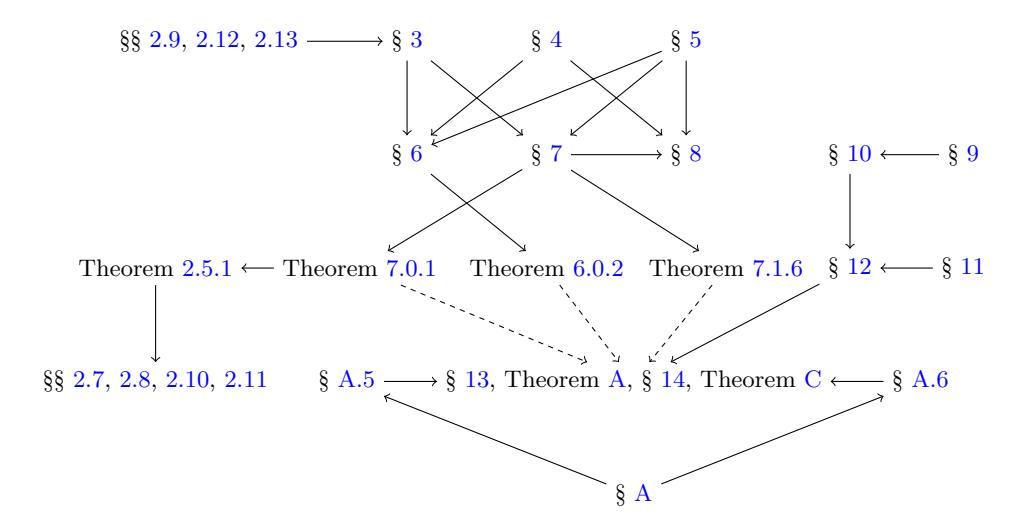
\includegraphics[width=0.6\textwidth]{assets/fig/CDT_L_2026_leitfaden.jpeg}
  \caption{导引图 (Leitfaden): 通往定理 A 和 C 的路径}\label{fig:1.3.0}
\end{figure}


% 引入第2节内容
\section{主算术 holonomy 边界}\label{sec:2}

我们首先在最简单的情况下讨论维度边界.

\subsection{代数情况}\label{sec:2.1}

我们对``无界分母''猜想的解决 \cite{CDT21} 是基于对代数函数的特定 $\mathbf{Q}(x)$-线性空间的如下维度上界估计.
我们将这种类型的结果称为算术 holonomy 边界 (arithmetic holonomy bound).
虽然这一名称在 \cite{CDT21} 中仍显晦涩, 但我们希望它能在本文中得到印证——在本文中, 我们处理更一般的 holonomic 函数, 其解析开拓产生无穷且不可解的单值群 (monodromy group).
给定闭单位圆盘 $\overline{\mathbf{D}} \subset \mathbf{C}$ 的某个邻域上的全纯映射 $\varphi: \overline{\mathbf{D}} \to \mathbf{C}$, 满足 $\varphi(0) = 0$ 且 $\lvert\varphi'(0)\rvert > 1$, 我们在 \cite[Theorem 2.1]{CDT21} 中确立了以下维度上界:
\begin{equation}\label{eq:2.1.1}
\dim_{\mathbf{Q}(x)} \mathcal{H}(\varphi) \le e \cdot \frac{\int_{\mathbf{T}} \log^{+} \lvert\varphi\rvert \, \mu_{\text{Haar}}}{\log \lvert\varphi'(0)\rvert}
\end{equation}
它作用于 $\mathbf{Q}(x)$-线性生成空间 $\mathcal{H}(\varphi)$ 上, 该空间由在 $\overline{\mathbf{D}}$ 的邻域上同样收敛的 $\mathbf{Z}[\! [x]\!]$ 形式幂级数 $f(x)$ 及其下拉 $\varphi$-pullback $f(\varphi(z))$ 生成.
这里 $\mathbf{T}$ 是单位圆, $\log^+\lvert x\rvert$ 定义为 $\max(0, \log\lvert x\rvert)$, 并且 $\mu_{\text{Haar}}$ 是 $\mathbf{T}$ 上的标准 Haar 测度, 
因此分子中的积分同样可以写为 $\int_0^1 \max(0, \log\lvert\varphi(e^{2\pi it})\rvert) dt$.

\begin{remark}[Basic Remark 2.1.2]\label{rem:2.1.2}
假设 \(f(x)\) 是一个幂级数, 它可以解析开拓为包含原点且共形映射半径 \(\rho(\Omega,0) > 1\) 的区域 \(\Omega \subset \mathbf{C}\) 上的全纯函数.
(关于共形映射半径的精确定义参见第 2.7 节开头.)
根据定义, 从而存在一个双全纯映射 \(\varphi : \mathbf{D} \to \Omega\), 满足 \(\varphi(0) = 0\) 且 \(\lvert\varphi'(0)\rvert = \rho(\Omega,0) > 1\).
反过来, \(f(x)\) 在 \(\Omega\) 上的全纯性恰恰意味着拉回的幂级数 \(f(\varphi(z)) \in \mathbf{C}[\![z]\!]\) 在 \(\mathbf{D}\) 上收敛.
边界估计 \eqref{eq:2.1.1} 随后表明, 由 \(f(x) \in \mathbf{Z}[\![x]\!]\) 及其各次幂生成的 \(\mathbf{Q}(x)\)-向量空间是有限维的 (因为 \(f(x)\) 的各次幂同样落入 \(\mathcal{H}(\varphi)\) 中), 
因而 \(f(x)\) 是代数函数 (具有某个显式有界的次数).
然而, 在这些假设下, 人们其实已经可以从 Borel--P{\'o}lya 定理 (即\autoref{thm:1.2.4}) 中推导出 \(f(x)\) 的有理性质.
因此, 当 \(\varphi\) 不是单值 (univalent) 时, 边界估计 \eqref{eq:2.1.1} 会更加有趣.
(我们最终会发现, Borel--P{\'o}lya 定理也将完全被比 \eqref{eq:2.1.1} 更精细的 holonomy 边界所吞并, 
例如下文源于 Bost--Charles \cite{BC22} 的边界 \eqref{eq:2.2.4}, 以及本文最终的新主 holonomy 边界 \eqref{eq:2.5.4}.)

一个非单值的例子如下. 
假设 \(f(x) \in \mathbf{Z}[\![x]\!]\) 可以解析开拓到从 \(0\) 出发且避开 \(0\) 和某个固定实数 \(\alpha > 0\) 的 \(\mathbf{C}\) 中的任意路径上.
例如, 取 \(f(x) = (1-4x)^{-1/2} = \sum {2n \choose n} x^n\), 且 \(\alpha = 1/4\).
则人们可以取 \(\varphi\) 为任何满足 \(\varphi(0) = 0\) 但不具有其他 \(0\) 或 \(\alpha\) 原像的全纯函数.
其中一个这样的函数是
\[ \varphi(z) = \alpha \lambda(z) \]
这里的 \(\lambda\) 是 \eqref{eq:1.2.8} 中给出的模 \(\lambda\) 函数.
在这种情况下, 我们有 \(\lvert\varphi'(0)\rvert = 16\alpha\).
因此, 如果 \(\alpha > 1/16\), 我们推导出 \(f(x)\) 是代数函数 (在 \(\mathbf{Q}(x)\) 上的次数具有由 \eqref{eq:2.1.1} 显式给出的界).
这个例子其实已经由 Andr{\'e} 给出.

论文 \cite{CDT21} 关注的是 \(\alpha = 1/16\) 的情况, 此时存在无穷多个 \(\mathbf{Q}(x)\)-线性无关的代数实例, 包括
\[ f(x) = \sum_{n=0}^{\infty} {4n \choose 2n} x^n = \sqrt{\frac{1 + \sqrt{1 - 16x}}{2 - 32x}}; \]
单在其上不添加任何条件，代数性将不再成立，这可以从超几何级数 \(\sum {2n \choose n}^2 x^n\) 中看出。
该例子曾被 Andr{\'e} 在 \cite{And96} 中使用, 并在 \cite{And04} 附录 A 中做了进一步讨论.
我们把关于代数情况的任何进一步讨论留给 \cite{CDT21}.

\end{remark}



\subsection{分母}\label{sec:2.2}

对于线性无关性证明, 正如第 1 节中的例子所暗示的, 我们需要作用于 \(\mathbf{Q}[\![x]\!]\) 上的 holonomy 边界, 而非 \(\mathbf{Z}[\![x]\!]\).
事实上, 我们这里作为首要关注点的有理系数——例如 \(\eta = L(2,\chi_{-3})\)——猜想上是超越数, 
因而任何在周期矩阵中的体现必然涉及一个具有无穷全球单值群 (global monodromy group)的局部系统.
另一方面, 如果 \(P(x) \in \mathbf{Z}[x]\) 落在附着于某个满足 \(\varphi(0) = 0\) 且 \(\lvert\varphi'(0)\rvert > 1\) 的 \(\varphi: \overline{\mathbf{D}} \to \mathbf{C}\) 的 holonomic 模 \(\mathcal{H}(\varphi)\) 中, 
那么就会推导出 \(P(x)\) 是代数函数.
Grothendieck--Katz 的 $p$-曲率猜想 \cite{And04} (已被 Katz 在许多源于几何的情形中证明) 非正式地将可积联络的全球单值群的无穷性与正密度素数 $p$ 下 $p$-曲率算子的非零性相对应——即模 $p$ 可积性的局部障碍.
但是我们提醒读者, 即使对于一个不可约的线性齐次 ODE, 
单个 \(\mathbb{Z}[1/S][\! [x]\!]\) 解并不意味着 $p$-曲率的消失; 
相反, \(\mathbb{Z}[1/S][\mathbf{x}^{1/h}]\) 的一组基解才意味着这一消失.
例如, 在第 1 节讨论的 Ap{\'e}ry 的论证中, 函数 \(A(x) \in \mathbb{Z}[x]\) 具有整系数但并不是代数函数.
为了将这个例子与上述关于 \(P(x)\) 的评述统一起来, 
请记住, holonomy 边界绝不是直接应用到 \(A(x) \in \mathbf{Z}[x]\) 本身, 
而是应用到同一个 ODE 的 A(x) 与另一个解 \(B(x) \in \mathbf{Q}[\![x]\!]\) 的某个设想用于引出矛盾的 \(\mathbf{Q}\)-线性组合 \(P(x) = B(x) - \eta A(x)\) 上.
这第二个解 \(B(x)\) 的系数分母中确实包含无穷多个素数.

由 \cite{And89}, 我们对源于 $G$-函数的泰勒级数 \(P(x) = \sum a_n x^n \in \mathbf{Q}[\![x]\!]\) 的分母类型具有一个猜想上的认识\footnote{对于“源于几何”的 $G$-函数而言, 这是一个无条件定理, 基于在除了有限个坏还原素数之外的所有素数处 $F$-晶体结构的存在性, 参见 \cite[§ V app.]{And89}. 我们可以更加精确: 如果对于某个非零的 $r$ 阶 Fuchsian 算子 $\mathcal{L}$ 有 $\mathcal{L}(f) = 0$, 且该算子在 $x = 0$ 处的局部指数为分母整除 $b$ 的有理数, 那么 $f$ 的分母形式可以取为 $A^{n+1}[1,\ldots,bn+b_0]^{r-1}$, 其中 $A \in \mathbb{N}_{>0}$ 且 $b_0 \in \mathbb{Z}$.}:
应当存在 \(A \in \mathbf{N}_{_{>0}}\), \(b \in \mathbf{Q}_{_{_{>0}}}\), 以及 \(\sigma \in \mathbf{N}\) 使得
\begin{equation}\label{eq:2.2.1}
a_n A^{n+1}[1, \dots, bn]^{\sigma} \in \mathbf{Z} \qquad \forall n \in \mathbf{N};
\end{equation}
这里以及在我们的整篇论文中 (正如之前在引言中指出的), [1, ..., n] 用于表示前 \(\lfloor n \rfloor\) 个正整数的最小公倍数.

最基本且常见的例子是 \(G\)-函数 \(\log(1-x)\). 
它的类型为 \eqref{eq:2.2.1} 并且满足 A=1, b=1 以及 \(\sigma=1\), 
但在这种情况下该形式显然可以被改进: 只需前 $n$ 个整数的最小公倍数级的分母消去能力即可, 这反映了以下事实:
\[ \log(1-x) = \int \frac{dx}{x-1} \]
是代数函数的积分. 
事实表明 (参见第 5 节), 利用这种源于积分的精细化表述最终将是以及重要的.
在任何情况下, 至少为 \([1, \dots, bn]\) 的分母的必要性迫使我们走出了形式算术表面理论 \cite{BC22} 的原有范畴\footnote{一个自然的框架是在形式解析算术簇及其代数化上构造和对比可积联络. 除了在 § 15.2 中提出一个特定的有限性问题之外, 我们不准备在本文中探讨这一概念, 但我们希望在其他场合重新讨论它.}.

在存在分母的情况下, 对于给定的全纯映射 \(\varphi : \mathbf{D} \to \mathbf{C}\) 以及参数 b \(\in \mathbf{Q}_{\ge 0}\) 和 \(\sigma \in \mathbf{N}\), 
我们定义 holonomic 模 \(\mathcal{H}(\varphi; b; \sigma)\) 为由以下形式的所有形式函数生成的 \(\mathbf{Q}(x)\)-线性空间:
\begin{equation}\label{eq:2.2.2}
f(x) = \sum_{n=0}^{\infty} a_n \frac{x^n}{[1, \dots, bn]^{\sigma}} \in \mathbf{Q}[\![x]\!], \qquad a_n \in \mathbf{Z} \quad \forall n \in \mathbf{N}
\end{equation}
且其 \(\varphi\)-下拉 \(f(\varphi(z))\) 在 \(\mathbf{D}\) 上收敛. 
\cite[§ 2]{CDT21} 中的证明可以常规地推广以确立这方面的第一个结果:
\begin{equation}\label{eq:2.2.3}
\dim_{\mathbf{Q}(x)} \mathcal{H}(\varphi; b; \sigma) \le e \cdot \frac{\int_{\mathbf{T}} \log^{+} \lvert\varphi\rvert \, \mu_{\text{Haar}}}{\log \lvert\varphi'(0)\rvert - \tau},
\end{equation}
这里 \(\tau := b\sigma\) 并且我们假设 \(\varphi\) 的共形大小满足 \(\lvert\varphi'(0)\rvert > e^{\tau}\).

不幸的是, 在 \cite{CDT21} 的渐近框架中表现良好的 holonomy 边界 \eqref{eq:2.2.3} (其中绝对数值系数并不重要), 
现在对于证明 \(L(2, \chi_{-3})\) 的无理数性质而言显得过于粗糙了.
因此, 探寻能够替代边界 \eqref{eq:2.2.3} 中常数 $e$ 的最小可能值是极有意义的.
Bost 和 Charles \cite[Corollary 8.3.5]{BC22} 取得了重大进展, 
他们在 \cite{CDT21} 的原始 \(\sigma = 0\) 的情况下, 确立了更精细的边界:
\begin{equation}\label{eq:2.2.4}
\frac{\iint_{\mathbf{T}^2} \log \lvert\varphi(z) - \varphi(w)\rvert \,\mu_{\text{Haar}}(z)\mu_{\text{Haar}}(w)}{\log \lvert\varphi'(0)\rvert}.
\end{equation}

在 2023 年, 为了响应我们关于对一般 holonomic 模 \(\mathcal{H}(\varphi; b; \sigma)\) 的类似维度边界的询问, 
Charles 向我们解释了他们的证明如何可以直接推广以得到:
\begin{equation}\label{eq:2.2.5}
\dim_{\mathbf{Q}(x)} \mathcal{H}(\varphi; b; \sigma) \le \frac{\iint_{\mathbf{T}^2} \log \lvert\varphi(z) - \varphi(w)\rvert \, \mu_{\mathrm{Haar}}(z) \mu_{\mathrm{Haar}}(w)}{\log \lvert\varphi'(0)\rvert - b\sigma}.
\end{equation}
这特别意味着 (例如参见\autoref{cor:8.1.14}) \eqref{eq:2.1.1} 和 \eqref{eq:2.2.3} 中的系数 $e$ 可以降为更好的常数 $2$.
Bost 和 Charles 的工作为我们探索无理数性质的应用提供了强有力的催化剂.
受 \cite{BC22} 的启发, 但走出了他们形式算术表面的框架, 并结合 Perelli 与 Zannier \cite{PZ84} 的一个想法, 
我们在附录 B 中证明了将 \eqref{eq:2.2.3} 中的 $e$ 降为 $2$ 的过程.
在第 7 节中, 我们基于 \cite{BC22} 中针对解析目的重新诠释的一些结果, 
将其进一步推向 Bost 先前的评估高度方法, 
以便将 \eqref{eq:2.2.4} 和 \eqref{eq:2.2.5} 推广到合并更精细的分母项; 
参见定理 2.5.1 获取第 7 节中我们边界的一个特例.
我们关于 2-进 $\zeta(5)$ 无理数性质的姐妹篇论文 \cite{CDT24} 在更广泛的背景中探索了这些边界.

\subsection{各种 holonomy 边界预览}\label{sec:2.3}

我们目前论文稳定的核心由精细化的 holonomy 边界组成, 这些边界改进了 \eqref{eq:2.2.5} 并统一了 \eqref{eq:2.2.3} 和 \eqref{eq:2.2.4} 背后的证明方法.
这些边界的一个方面是改进了 \eqref{eq:2.2.3} 中的 \(\tau = b\sigma\) 项; 
在这里, 高维方法最终提供了更精确的信息, 尽管这种差异在本文的所有应用中是隐而不现的.
另一个方面是进行更精细的复分析估计 (参见第 2.13.10 节和第 2.13.13 节获取思想概述) 
以进一步改进 \eqref{eq:2.2.4} 中的双重积分; 
这里的改进在单变量中与在高维处理中是完全相同的.
其中一项技术新颖性是引入了来自大偏差理论 (large deviations theory) 的概率输入, 
即使在我们 \cite[§ 2]{CDT21} 原始多元分析的初等多元框架中, 
它也能容纳将系数从 $e$ 降为 $2$ 的改进.
这是通过在 $d$ 个辅助变量中的双廷逼近论证确立的, 
而在这一高维几何特征的极限过程 $d \to \infty$ 中, 
精确实现系数从 $e$ 降为 $2$ 的改进之关键在于, 它为进一步的独立改进提供了额外的空间.
我们在本文中拥有的最尖锐的 holonomy 边界 (定理 8.0.1) 是高维评估模中测度集中特征的产物.

对于本文中的应用（包括定理 A 和 C），分母项最精细的改进其实并没有带来差别.
我们为这些定理提供了两条通用的简化路径.
一条是通过定理 6.0.2 在基本的 Siegel 引理框架中使用高维技术, 
而另一条是通过定理 7.0.1 并且可选择定理 7.1.13 使用单变量方法.
(参见第 1.3 节了解本文不同章节之间依赖关系的更多细节, 以及通往定理 A 和 C 的各种路径.)
对于定理 A 的应用, 定理 7.0.1 给出了最弱的勉强合格边界（仅具有微弱的盈余）, 
而其``凸性精细化''形式（定理 7.1.10）则给出了比它们中任何一个都更强的边界.
定理 7.0.1 的证明是 Bost 与 Charles 工作的直接结合, 
并伴随着我们对相对简单设定中 \(\tau = b\sigma\) 项的改进 (参见定理 2.5.1; 这一简单设定使得我们即使不用高维方法也能获得 \(\tau\) 的最佳改进), 
以及第 5 节中用于容纳分母类型 \eqref{eq:2.2.1} 中 $n$ 的额外方幂的计算.

为了获得能以更充裕盈余处理定理 A 的更强边界, 我们使用更精细的复分析估计来证明定理 6.0.2 和定理 7.1.6.
在前者的情况下, 大偏差输入不仅用于达到分母速率项 \(\tau\) 的改进, 
而且还用于将 Bost--Charles 双重积分替换为我们在第 2.4 节中引入的更初等的重排积分\footnote{这里的重排积分指的是比 $\int_0^1 2t \cdot (\log \lvert\varphi(e^{2\pi it})\rvert)^* dt$ 的被积函数中的 $\log \lvert\varphi\rvert$ 更一般的函数集合. 正如我们将在 § 8.1 中看到的, 后者比 Bost--Charles 双重积分更大. 一般来说, 我们通过使用一组促进我们精细化复分析估计的合适半径 $r$, 将该被积函数内部的 $\varphi$ 替换为函数 $z \mapsto \varphi(rz)$ 的分段加权组合.}; 
这里的证明完全独立于 \cite{BC22}.
另一方面, 基于 \cite{BC22} 和定理 7.0.1, 我们对 Bost 斜率框架中评估映射高度的最佳估计进行了更仔细的研究, 
并利用这些改进来证明定理 7.1.6. 
这就是我们所谓的``来自凸性的改进'', 这一命名术语指的是亚纯函数值分布理论中的一个经典定理: 
亚纯函数 \(\varphi\) 的 Nevanlinna 特征函数 \(T(r,\varphi)\) 是 \(\log r\) 的凸递增函数.
此外, 如果我们在辅助多项式的评估模上选择某种启发式最佳的 Hermitian 结构, 
定理 7.1.6 的论证将引出启发式最佳的边界, 我们将其表述为定理 7.6.4, 这依然使用单变量方法.
在我们在下文引言定理 2.5.1 中引入的基本分母上限中, 定理 7.6.4 与定理 8.0.1 相同 (参见注记 8.0.6), 
并且我们预期 (参见注记 7.6.7) 两者都给出比定理 6.0.2 更强的边界.

我们现在继续描述这些基本改进中的一部分, 然后给出我们新 holonomy 边界的第一种形式.

\subsection{Nevanlinna 生长特征的变体}\label{sec:2.4}

从起始边界 \eqref{eq:2.2.3} 出发, 在进一步探讨 \cite[Remark 2.3.3]{CDT21} 时, 
多变量自然地将 Nevanlinna 的生长特征项 \(\int_0^1 \log^+ \lvert\varphi(e^{2\pi i t})\rvert dt\) 
改进为明显更小的重排积分 \(\int_0^1 t \cdot (\log \lvert\varphi(e^{2\pi i t})\rvert)^* dt\); 
这里以及在我们的整篇论文中, 我们遵循经典分析的惯例, 用
\begin{equation}\label{eq:2.4.1}
g^{*}(t) := \inf_{s \in \mathbf{R}} \left\{ \mathbf{P} \left( x \in (0,1) : g(x) > s \right) \le t \right\} = \inf_{s \in \mathbf{R}} \left\{ \int_{0}^{1} \chi_{g^{-1}([s,\infty))} dt \le t \right\}
\end{equation}
来表示可测函数 \(g:(0,1)\to \mathbf{R}\) 的递增重排 (increasing rearrangement).
(参见基本注记 2.4.4.) 
这是唯一的\footnote{在忽略测度为零的集合之外相差一个函数的意义下. 一些作者更喜欢使用“非降重排函数”这一术语.}与 g 具有相同分布函数的非递减可测函数.
\begin{equation}\label{eq:2.4.2}
\int_0^1 2t \cdot g^*(t) \, dt = \int_0^1 \int_0^1 \max(g(s), g(t)) \, ds \, dt,
\end{equation}
这引出了与来自 \eqref{eq:2.2.4} 的 Bost--Charles 双重积分项的对比.
\(\varphi\) 在圆周上的积分行为在第 8.1 节将被详细研究, 并且我们将会发现它比后者稍微大一些.

然而, 正是 \eqref{eq:2.4.2} 的左手边自然地呈现在我们新论证的概率论特征中.
对于我们这里的讨论, 只需注意到以下平凡的不等式:
\begin{equation}\label{eq:2.4.3}
\int_0^1 2t \cdot g^*(t) \, dt \le \int_0^1 2 \max(g^*(t), 0) \, dt = \int_0^1 2 \max(g(t), 0)^* \, dt = 2 \int_0^1 \max(g(t), 0) \, dt
\end{equation}
它适用于任何可测函数 g, 
因而这特别在更广泛的高维视角下恢复了系数从 $e$ 降为 $2$ 的改进, 
这在某种意义上是一种与 \cite{BC22} 或第 7 节中任何一个单变量分析``正交''的方法.
(这些单变量分析方法具有 Arakelov 几何的特征, 
并带有它们自身且各不相同的对 Nevanlinna 生长特征的精细化表述, 
这在第 7.1.1 节中我们将其称为 Bost--Charles 特征.) 
现在的关键点在于, 这一极限过程 $d \to \infty$ 的论证进一步允许了对 \eqref{eq:2.2.3} 到 \(\mathbf{Q}[\! [x]\!]\) 函数的推广中 \(\tau = b\sigma\) 项进行类似的``分母递增重排''改进.
某种这样的改进对于我们定理 A 和 C 的所有证明都是必不可少的.
我们确实也在第 7 节中对第 6 节的主要结果给用了单变量处理.

\begin{remark}[基本注记 2.4.4]\label{rem:2.4.4}
理解等式 \eqref{eq:2.4.1} 中 $g^*(t)$ 的定义的一个基本方法如下. 
假设 $g(t)$ 是 $[0, 1]$ 上的连续 (从而有界) 函数. 如果 $g(t)$ 是单调递增的, 那么 $g^*(t) = g(t)$. 对于任意的 $g(t)$, 设 $g_n(t)$ (对于 $n \ge 1$) 表示分段常数阶梯函数, 
它在区间 $I_k = [(k-1)/n, k/n)$ (对于 $k = 1, \ldots, n$, 并将最后一个区间 $I_n$ 延伸至包含 1) 上取值为 $g(k/n)$. 当 $n \to \infty$ 时, 函数 $g_n(t)$ 一致收敛于 $g(t)$. 现在设 $g_n^*(t)$ 表示同样在这 $n$ 个区间 $I_1, \ldots, I_n$ 上为常数的阶梯函数, 
只是现在分别取这 $n$ 个对应值 $\{g(1/n), g(2/n), g(3/n), \dots, g(n/n)\}$ 并在重新进行递增排序 (因此得名). 
那么 $g_n^*(t)$ 就是 $g_n(t)$ 的递增重排, 
并且函数 $g_n^*(t)$ 当 $n \to \infty$ 时一致收敛于 $g^*(t)$. \end{remark}

\subsection{算术 holonomy 边界，基本形式}\label{sec:2.5}

\begin{theorem}\label{thm:2.5.1}
考虑两个正整数 \(m, r \in \mathbf{N}_{>0}\) 以及一个非负实数组成的 \(m \times r\) 矩形阵列 \(\mathbf{b} := (b_{i,j})_{1 \le i \le m, 1 \le j \le r}\), 其所有列均具有如下形式:
\[ 0 = b_{1,j} = \dots = b_{u_j,j} < b_{u_j+1,j} = \dots = b_{m,j} =: b_j, \qquad \forall j = 1,\dots,r, \]
对于某些 \(u_j \in \{0, 1, \dots, m\}\). 令
\[ \sigma_i := b_{i,1} + \dots + b_{i,r}, \qquad i = 1, \dots, m \]
为第 \(i\) 行之和, 并且定义
\begin{equation}\label{eq:2.5.2}
  \tau(\mathbf{b}) := \frac{1}{m^2} \sum_{i=1}^{m} (2i - 1)\sigma_i = \sigma_m - \frac{1}{m^2} \sum_{j=1}^{r} u_j^2 b_j \in [0, \sigma_m].
\end{equation}
此外, 考虑一个全纯映射 \(\varphi: (\overline{\mathbf{D}}, 0) \to (\mathbf{C}, 0)\), 其导数 (共形大小) 满足 \(\lvert\varphi'(0)\rvert > e^{\sigma_m}\).
假设存在一个由在 \(\mathbf{Q}[\! [x]\!]\) 中的 \(\mathbf{Q}(x)\)-线性无关形式函数组成的 \(m\)-元组 \(f_1, \dots, f_m\), 它们的分母类型为如下形式:
\begin{equation}\label{eq:2.5.3}
  f_i(x) = \sum_{n=0}^{\infty} a_{i,n} \frac{x^n}{[1, \dots, b_{i,1} \cdot n] \cdots [1, \dots, b_{i,r} \cdot n]}, \qquad a_{i,n} \in \mathbf{Z},
\end{equation}
使得对于所有 \(i = 1, \dots, m\), 其拉回 \(f_i(\varphi(z)) \in \mathbf{C}[\![z]\!]\) 是在 \(|z| < 1\) 上的亚纯函数的芽 (germ).
那么我们有以下边界:
\begin{equation}\label{eq:2.5.4}
  m \le \frac{\iint_{\mathbf{T}^2} \log \lvert\varphi(z) - \varphi(w)\rvert \, \mu_{\text{Haar}}(z) \mu_{\text{Haar}}(w)}{\log \lvert\varphi'(0)\rvert - \tau(\mathbf{b})}.
\end{equation}
此外, 如果先验地假设所有函数 \(f_i\) 都是全纯的, 则条件 \(\lvert\varphi'(0)\rvert > e^{\sigma_m}\) 可以放宽为 \(\lvert\varphi'(0)\rvert > e^{\tau(\mathbf{b})}\).
\end{theorem}

利用基于高维测度集中现象的初等方法, 我们在第 6 节中直接证明了以下使用递增重排函数的变体:
\begin{equation}\label{eq:2.5.5}
m \le \frac{\iint_{\mathbf{T}^2} \log \left( \max(\lvert\varphi(z)\rvert, \lvert\varphi(w)\rvert) \right) \, \mu_{\mathrm{Haar}}(z) \mu_{\mathrm{Haar}}(w)}{\log \lvert\varphi'(0)\rvert - \tau(\mathbf{b})} = \frac{\int_0^1 2t \cdot (\log \lvert\varphi(e^{2\pi it})\rvert)^* \, dt}{\log \lvert\varphi'(0)\rvert - \tau(\mathbf{b})}.
\end{equation}

为了突出 \(\tau(\mathbf{b})\) 与简单概率考量中出现的递增重排函数的相似性，我们可以写出以下形式的等价加权积分表示（设 \(\sigma_0 := 0\)）：
\begin{equation}\label{eq:2.5.6}
\tau(\mathbf{b}) = \sum_{i=1}^{m} \sigma_i \int_{(i-1)/m}^{i/m} 2t \, dt = \int_0^1 2t \cdot \left( \sum_{i=1}^{m} (\sigma_i - \sigma_{i-1}) \chi_{[0,i/m]}(t) \right) \, dt.
\end{equation}

\subsection{Siegel 的 $G$-函数}\label{sec:2.6}

正如上文所讨论的, \autoref{thm:2.5.1} 具有一个粗糙的定性推论, 我们可以将其解读为算术 holonomicity 判定准则. 它由 Andr{\'e} 在 \cite{And89} 中给出; 在稍有不同的语境中, 这一类型的第一个全纯性结果大概是由 Perelli 和 Zannier 在 \cite{PZ84} 中发现的.

\begin{corollary}\label{cor:2.6.1}
如果一个形式函数 \(f \in \mathbf{Q}[\! [x]\!]\) 具有如下形式的有理系数:
\begin{equation}\label{eq:2.6.2}
  f(x) = \sum_{n=0}^{\infty} a_n \frac{x^n}{[1, \dots, b_1 n] \cdots [1, \dots, b_r n]}, \qquad a_n \in \mathbf{Z}
\end{equation}
并且允许一个满足共形大小 \(\lvert\varphi'(0)\rvert > e^{b_1 + \dots + b_r}\) 的全纯映射 \(\varphi: (\mathbf{D}, 0) \to (\mathbf{C}, 0)\), 使得复合函数芽 \(f(\varphi(z)) \in \mathbf{C}[\![z]\!]\) 成为 \(\mathbf{D}\) 上的亚纯函数的芽, 
那么 \(f(x)\) 是一个 holonomic 函数: 存在一个非零且在 \(\mathbf{Q}[x]\) 中具有系数的线性微分算子 \(\mathcal{L}\) 满足 \(\mathcal{L}(f) = 0\).
\end{corollary}

在本文中, 我们将展示并利用这样一些 $f \in \mathbf{Q}[\![x]\!]$，其 holonomic 性质可以通过该准则进行识别。分母 \eqref{eq:2.6.2} 的特殊形式将我们更具体地置于 Siegel 的 $G$-函数理论语境中；特别是，参见注记 3.2.12 进行的讨论，线性微分算子 $\mathcal{L}$ 事后可以被视作属于 Fuchsian 类，仅具有正则奇点且具有有理指数 \cite[III 6.1, VII 2.1, 和 VIII 1.5]{DGS94}。一个重大的未决问题（这与 § 15.2 的讨论密切相关，且对无理数证明及有效的 Siegel 整点问题有重要影响）是控制在极小阶非齐次常微分方程 $\mathcal{L}(f) \in \mathbf{Q}[x]$ 中线性微分算子 $\mathcal{L}$ 可能出现的表观奇点（apparent singularities）。

\begin{remark}[Basic Remark 2.6.3]\label{rem:2.6.3}
最简单的例子是 $f(x) = \log(1-x)$, 它的类型由 $(b_1, \ldots, b_r) = (1)$ 给出，且极小微分算子为 $\mathcal{L} := (1-x)(d/dx)^2 - (d/dx)$，它在区域 $\Omega = \mathbb{C} \setminus \{1\}$ 上 holonomic 地变化，从而定义了一个二阶局部系统
\[ \operatorname{Span}_{\mathbf{C}} \{ 1, \log(1-x) \} \]
其围绕奇点 $x=1$ 的单值群（monodromy group）是由单能矩阵（unipotent matrix）
\begin{equation*}
T := \left( \begin{array}{cc} 1 & 0 \\ -2\pi i & 1 \end{array} \right)
\end{equation*}
生成的无限循环群。
这表达了这样一个事实：在沿着包围奇点 $\{1\}$ 的逆时针简单闭回路上解析开拓 $T$（局部单值算子）时，对于 $\log(1-x)$ 保持 $f_1 := 1$ 不变，但会为 $f_2 := \log(1-x)$ 加上周期 $-2\pi i$ 乘以 $f_1$：
\begin{equation*}
T^{k}(\log(1-x)) = \log(1-x) - 2\pi i k, \qquad T^{k}(1) = 1.
\end{equation*}
此外，该 holonomic 例子也能够被识别为属于全纯性准则推论 2.6.1 的一种情形。例如，在多值映射选择下，对于任意 $R > e$ 可取 $\varphi(z) := 1 - e^{-Rz}$；或取满射性质的 $\varphi(z) := \lambda(z)$，其导数满足 $|\varphi'(0)| = 16 > e$；或在单值选择下取 $\varphi(z) := 4z/(1+z)^2$，其导数满足 $|\varphi'(0)| = 4 > e$。

在定理 2.5.1 中，分母类型被捕获为一个 $2 \times 1$ 的矩阵 $\mathbf{b} = (0,1)^{\mathrm{t}}$，且满足 $\tau(\mathbf{b}) = (1 \cdot 0 + 3 \cdot 1)/2^2 = 3/4$。对于映射选择 $\varphi(z) := 4z/(1+z)^2$，其 holonomy 商值约等于 $\log 4/(\log 4 - 3/4) \approx 2.1787$，它是该二阶局部系统维数 $m=2$ 的一个维度上界估计。
\end{remark}

在第 11 节中，我们将对 Zagier 的 holonomic 函数 \cite{Zag09} 进行彻底研究，这些函数同样将数值 $\zeta(2)$ 和 $L(2,\chi_{-3})$ 赋予为分布在更复杂区域 $\Omega = \mathbb{C} \setminus \{0,1/9,1\} \cong \mathbb{H}/\Gamma_0(6)$ 上的局部系统中的周期。对于这一局部系统（它源于分析 Ap{\'e}ry 关于 $\zeta(2)$ 无理性证明 \cite{Ape79}\cite{Coh78}\cite{vdP79} 中的递推形式，并基于 Eichler 积分理论），我们现在将拥有主整性类型 $x^n/[1,\ldots,n]^2$。随后，我们将把 $1, \zeta(2), L(2,\chi_{-3})$ 的 $\mathbf{Q}$-线性无关性问题归结为一个关于不存在类型为 $x^n/[1,\ldots,n]^2$ 且具有某些解析性质的 $G$-函数的丢番图分析问题：具体而言，我们的任务转为证明 Zagier 的局部系统不能包含在奇点 $\{0,1/9\}$ 处正则（即 $e_0$ 超收敛）的非零 $\mathbb{Q}[x]$ 元素。

直接应用 \eqref{eq:2.5.4}（参见本节下文的第 2.11 节）足以证明如下混合周期的无理数性质：
\begin{equation*}
L(2,\chi_{-3}) - \pi \frac{\log 3}{3\sqrt{3}} = L(2,\chi_{-3}) - L(1,\chi_{-3}) \log 3.
\end{equation*}

（另一个关于混合周期的无理性结果是 Beukers 利用模形式证明的 $\zeta(3) - 5\sqrt{5} L(3, \chi_5) \notin \mathbf{Q}(\sqrt{5})$ \cite[Thm 4]{Beu87}。）为了证明纯 $L(2, \chi_{-3})$ 的无理性（如 § 2.3 中所讨论的），我们需要一个甚至比这更精细的结果，以同时考虑函数的积分。这些更复杂的定理 2.5.1 版本（包括定理 6.0.2、7.0.1、7.1.6 和 7.1.13）将被推迟到下文第 6 节与第 7 节中进行证明。向定理 A 的具体应用相当微妙，在产生 $\zeta(2)$ 和 $L(2, \chi_{-3})$ 作为其 holonomic 系数的众多局部系统中，最终对我们起作用的选择是高度可约的（尽管具有不可解的单值群），并且涉及导致分母本质上\footnote{更准确地说，是具有 $n[1, ..., 2n+3]^2$ 的形式，但根据注记 6.0.12，这或多或少可以被视作具有 $n[1, ..., 2n]^2$ 的形式。}为 $n[1, \ldots, 2n]^2$ 形式的积分。

\subsection{单值 holonomy 边界与对数的算术特征}\label{sec:2.7}

我们现在考虑将 \autoref{thm:2.5.1} 特殊化到映射 \(\varphi\) 为单值的情形. 我们指出, 尽管对于一般的 \(\varphi\), 我们拥有对 \autoref{thm:2.5.1} 的各种改进, 比如定理 7.1.6 和定理 7.6.4 (在假设其对应部分中的 $\mathbf{e}$ 为 $\mathbf{0}$ 的情况下), 但在 \(\varphi\) 为单值的情况下, 所有这些都将简化为如下的\autoref{thm:2.7.1}.

对于包含原点的单连通区域 \(\Omega \subset \mathbf{C}\), 黎曼映射定理提供了一个双全纯映射 \(\varphi : \mathbf{D} \xrightarrow{\simeq} \Omega\), 满足 \(\varphi(0) = 0\), 由 Schwarz 引理, 该映射在一圈旋转的意义下是唯一确定的. 这使得绝对值 \(\lvert\varphi'(0)\rvert \in (0,\infty]\) 是良好定义的; 我们用 \(\rho(\Omega,0)\) 表示它并将其称为单连通区域在原点处的共形映射半径. 如果全纯映射 \(\varphi : \mathbf{D} \to \mathbf{C}\) 是单值 (univalent) 的, 则称其为其图像上的双全纯映射, 或者等价地, 如果 \(\varphi : \mathbf{D} \hookrightarrow \mathbf{C}\) 是单射.

\begin{theorem}[Univalent Holonomy Bound]\label{thm:2.7.1}
在\autoref{thm:2.5.1} 的记号与假设下, 考虑一个单连通区域 \(\Omega \subset \mathbf{C}\), 满足 \(0 \in \Omega\) 且具有满足 \(\rho(\Omega,0) > e^{\tau(\mathbf{b})}\) 的共形映射半径. 对于任意一个在 \(\Omega\) 上是亚纯的、由 \(\mathbf{Q}(x)\)-线性无关的类型为 \eqref{eq:2.5.3} 的形式函数组成的 \(m\)-元组, 以下 holonomy 边界成立:
\[ m \le \frac{\log \rho(\Omega, 0)}{\log \rho(\Omega, 0) - \tau(\mathbf{b})}. \]
\end{theorem}

\begin{proof}
这直接由\autoref{thm:2.5.1} 导出. 
需要观察的关键点是, Bost--Charles 双重积分项满足不等式:
\begin{equation*}
\iint_{\mathbf{T}^2} \log |\varphi(z) - \varphi(w)| \, \mu_{\mathrm{Haar}}(z) \mu_{\mathrm{Haar}}(w) \ge \log |\varphi'(0)|,
\end{equation*}
其中等号成立当且仅当 \(\varphi : \mathbf{D} \hookrightarrow \mathbf{C}\) 在开圆盘上是单值的. 
为了说明这一点, 只需注意到单值性等价于双变量全纯函数
\[ \frac{\varphi(z) - \varphi(w)}{z - w} = \varphi'(0) + O(|z| + |w|) \in \mathcal{O}(\mathbf{D}^2) \]
在整个单位多圆盘内非零. 
因此, 函数
\[ G(z,w) := \log \left| \frac{\varphi(z) - \varphi(w)}{z - w} \right| : \mathbf{D}^2 \to \mathbf{R} \cup \{-\infty\} \]
是多重次调和的 (plurisubharmonic), 并且其为调和函数当且仅当 \(\varphi\) 是单值的. 
注意到 \(G(0,0) = \log |\varphi'(0)|\), 同时根据基本积分恒等式 \(\iint_{\mathbf{T}^2} \log \frac{1}{|z-w|} \mu_{\text{Haar}}(z) \mu_{\text{Haar}}(w) = 0\), 有
\[ \iint_{\mathbf{T}^2} G(z, w) \, \mu_{\text{Haar}}(z) \mu_{\text{Haar}}(w) = \iint_{\mathbf{T}^2} \log |\varphi(z) - \varphi(w)| \, \mu_{\text{Haar}}(z) \mu_{\text{Haar}}(w), \]
由此上述两个断言均得证.
\end{proof}

我们指出以下将\autoref{thm:2.7.1} 应用到对数函数的情形, 这正是基本注记 2.6.3 的例子.

\begin{theorem}\label{thm:2.7.2}
假设 \(f(x) = \sum_{n=0}^{\infty} a_n x^n \in \mathbf{Q}[\! [x]\!]\) 是一个幂级数, 满足:
\begin{enumerate}
  \item[(1)] 对于所有 \(n \in \mathbf{N}\), \([1, \dots, n]a_n \in \mathbf{Z}\).
  \item[(2)] \(f(x)\) 在 \(\mathbf{C} \setminus [1, \infty)\) 上是全纯的.
\end{enumerate}
那么
\[ f(x) = Q_0(x) + Q_1(x)\log(1-x) \]
对于某些有理函数 \(Q_0, Q_1 \in \mathbf{Q}\left[x, \frac{1}{1-x}\right] \subset \mathbf{Q}(x)\) 成立.
\end{theorem}

我们视\autoref{thm:2.7.2} 为对数函数的一个算术特征刻画.

\begin{proof}
我们考虑收缩区域 \(\Omega := \mathbb{C} \setminus [1, \infty)\), 其在原点处的共形映射半径为 \(\rho(\Omega,0)=4\), 对应的黎曼映射为 \(\varphi(z)=4z/(1+z)^2\). 
我们在 \(m=3\), \(r=1\) 且 \(\mathbf{b}=(0,1,1)^{\mathrm{t}}\) 满足 \(\tau(\mathbf{b})=8/9\) 的情况下应用\autoref{thm:2.7.1}, 此时数值计算
\begin{equation}\label{eq:2.7.3}
\frac{\log 4}{\log 4 - 8/9} = 2.787050 \dots < 3
\end{equation}
证明了不存在第三个 \(\mathbf{Q}(x)\)-线性无关的、类型为 \eqref{eq:2.6.2} 且在 \(\Omega = \mathbb{C} \setminus [1, \infty)\) 上解析的函数, 它与两个已知的例子 \(f_1 = 1\) 和 \(f_2 = \log(1-x)\)（其对应 \((b_1, \ldots, b_r) = (1)\)）线性无关. 
这意味着所有此类函数必定具有 \(Q_0(x) + Q_1(x) \log(1-x)\) 的形式, 其中 \(Q_0(x), Q_1(x) \in \mathbf{Q}(x)\).

此时, 我们已知 \(f(x)\) 在 \(\mathbb{C} \setminus ([1, \infty) \cap \overline{\mathbb{Q}})\) 上是正则（全纯）的, 并且 \(\mathbf{C}\) 中的每个点 \(x \neq 1\) 至多是 \(f(x)\) 的一个亚纯极点. 接下来只需证明以下两点:
\begin{itemize}
  \item[(i)] \(Q_0(x)\) 和 \(Q_1(x)\) 属于 \(\mathbf{Q}(x)\) 的子环 \(\mathbf{Q}\left[x, \frac{1}{x}, \frac{1}{1-x}\right]\).
  \item[(ii)] 如果 \(Q_0(x), Q_1(x) \in \mathbf{Q}[x, 1/x]\), 则必定有 \(Q_0(x), Q_1(x) \in \mathbf{Q}[x]\).
\end{itemize}
事实上, 假定 (i) 成立, 我们只需将 \(f(x)\) 替换为 \((1-x)^k f(x)\)（其中 \(k \in \mathbb{N}\) 是一个足够大的次数以消去 \(Q_0(x)\) 中的分母 \((1-x)\)）, 那么由 (ii) 即可得出我们所需的结论.

我们首先证明 (ii). 假设 \(Q_0(x)\) 和 \(Q_1(x)\) 不都在 \(\mathbf{Q}[x]\) 中. 如果
\[ Q_1(x) \in \mathbf{Q}[x] \subset (1/x)\mathbf{Q}[x] \]
那么 \(Q_1(x) \log(1-x)\) 在 \(x=0\) 处是全纯的, 从而 \(Q_0(x)=f(x)-Q_1(x)\log(1-x)\) 在 \(x=0\) 处也是全纯的, 进而 \(Q_0(x)\in \mathbf{Q}[x]\). 
因此我们可以假设 \(Q_1(x) \in \mathbf{Q}[x, 1/x] \setminus \mathbf{Q}[x]\). 
在将 \(f(x)\) 乘以适当的 \(x\) 的幂次以及足够整除的正整数之后, 我们可以假设 \(Q_1(x) \in (\mathbf{Z}[x] + \mathbf{Z} \cdot x^{-1}) \setminus \mathbf{Z}[x]\) 并且 \(Q_0(x)\)（根据上述参数, 它现在也是全纯的）属于 \(\mathbf{Z}[x, 1/x]\) 从而也属于 \(\mathbf{Z}[x]\), 且此时分母性质 (1) 依然保持. 
反过来, 通过从 \(f(x)\) 中减去 \( \mathbf{Z}[x] + \log(1-x)\mathbf{Z}[x] \) 中的适当元素, 我们只需分析如下情况
\[ f(x) = \frac{q_1 \log(1-x)}{x} \]
其中 \(q_1 \in \mathbf{Z} \setminus 0\). 
但在这种情况下, \(f(x)\) 的 \(x^{p-1}\) 项系数等于 \(q_1/p\), 当 \(p > |q_1|\) 为素数时, 这显然不满足所需的性质 (1). 这完成了化简步骤 (ii).

我们现在考虑 (i). 假设有理函数 \(Q_0(x)\) 和 \(Q_1(x)\) 不属于子环 \(\mathbf{Q}\left[x, \frac{1}{x}, \frac{1}{1-x}\right]\), 那么其中至少一个必定有一个极点 \(\alpha \in \overline{\mathbf{Q}} \setminus \{0, 1\}\).

固定一个复嵌入 \(\overline{\mathbf{Q}} \hookrightarrow \mathbf{C}\), 首先考虑对于 \(Q_0(x)\) 或 \(Q_1(x)\) 的至少一个极点满足 \(\alpha \notin (1, \infty)\) 的情形. 
在这种情况下, 我们关于 \(f(x)\) 在 \(\alpha\) 处全纯的假设意味着
\[ Q_0(x) = \frac{V(x)}{(x-\alpha)^k}, \quad Q_1(x) = \frac{-U(x)}{(x-\alpha)^k} \]
对于某个正整数 \(k \in \mathbb{N}_{>0}\) 以及在 \(x = \alpha\) 处正则且不为零的有理函数 \(U, V \in \overline{\mathbb{Q}}(x)\) 成立. 
在等式
\[ (x - \alpha)^k f(x) = V(x) - U(x)\log(1 - x) \]
中代入 \(x = \alpha\), 得到一个非平凡的消去组合 \(V(\alpha) - U(\alpha) \log(1 - \alpha) = 0\), 其系数为非零代数数 \(U(\alpha), V(\alpha) \in \overline{\mathbf{Q}}^{\times}\). 
但这与 Hermite--Lindemann--Weierstrass 关于 \(\log(1-x)\) 在 \(\overline{\mathbf{Q}} \setminus \{0,1\}\) 上的代数自变量取超越值的定理相矛盾.

剩下的情况是 \(Q_0\) 和 \(Q_1\) 的所有非 \(0, 1, \infty\) 的极点 \(\alpha\) 都属于 \(\alpha \in (1, \infty) \cap \overline{\mathbf{Q}}\), 且这一极点集合非空. 
此时, 我们的全纯性条件 \(f \in \mathcal{O}(\mathbf{C} \setminus [1, \infty))\) 并不能排除在 \(x = \alpha\) 处的亚纯极点, 因而我们需要一个不同的论证. 
由于所讨论的极点集合在 \(\mathrm{Gal}(\overline{\mathbf{Q}}/\mathbf{Q})\) 作用下是稳定的, 我们的假设意味着 \(\alpha\) 的所有 Galois 共轭也必定落在 \((1, \infty) \cap \overline{\mathbf{Q}}\) 中. 
那么我们根据乘积公式可以推导出, 存在一个素数 \(p\) 以及极点的一个选择 \(\alpha \in \overline{\mathbf{Q}} \cap \mathbf{C}_p\), 使得它落在开圆盘 \(|x|_p < 1\) 中. 
接着, 引用 Mahler 关于 \(p\)-进指数函数在非零代数自变量处所有收敛值超越性的定理 \cite{Mah19a}, 我们可以在 \(p\)-进意义下得到同样的矛盾; 
该定理等价于 \(p\)-进对数函数 \(\log(1-x)\) 在去心开单位圆盘 \(0 < |x|_p < 1\) 的代数点处的所有取值均为超越数.\footnote{\(p\)-进下关于指数函数特殊值代数无关性的完整 Hermite--Lindemann--Weierstrass 定理的对应结论是一个著名且尚未解决的猜想. 我们参考 Nesterenko 的工作 \cite{Nes08} 以获取部分结果, 并参考 \cite[§ 2.4]{Nes19} 以对该主题进行概述并对 Mahler 的论证作一介绍.}
\end{proof}

\begin{remark}[Remark 2.7.4]\label{rem:2.7.4}
\autoref{thm:2.7.2} 及其证明在将 (1) 减弱为例如下述形式时依然成立:
\[ \left[1,\ldots,\left(1+\frac{1}{100}\right)n\right]; \]
但此时仅能通过步骤 (i) 得到较弱的结论 \(Q_0, Q_1 \in \mathbf{Q}[x, 1/x, 1/(1-x)]\), 此时 \(1/x\) 确实无法再被消去, 对应实例有函数 \(f(x) = 100! \cdot \log(1-x)/x\). 
这里的常数 \(1 + 1/100\) 也可以等价地替换为区间 \((1, (3 \log 2)/2) = (1, 1.03972\dots)\) 中的任意元素.
\end{remark}

\begin{remark}[Remark 2.7.5]\label{rem:2.7.5}
在\autoref{thm:2.7.2} 的结论中, 我们能完全刻画所有可能的 \(Q_i(x)\). 
具体而言, \(f(x) = Q_0(x) + Q_1(x) \log(1-x)\) 具有所需形式的充要条件为以下两个条件同时成立:
\begin{enumerate}
  \item[(1)] \(Q_1(x) \in \mathbf{Z}[x, 1/(1-x)]\).
  \item[(2)] 对于每个 \(n\), \(Q_0(x)\) 属于由 \(x^n/[1, \dots, n]\) 生成的 \(\mathbf{Z}[x, 1/(1-x)]\)-模; 这等价于由每个素数幂 \(q\) 对应的 \(x^q/q\) 生成.
\end{enumerate}
这给出了\autoref{thm:2.7.2} 中（无限维）解的 \(\mathbf{Z}[x, 1/(1-x)]\)-模的生成元与关系的完整描述.

显然, 这些条件蕴含了\autoref{thm:2.7.2} 的要求. 
为了证明其逆命题, 考虑定理中满足 \(f(x) = Q_0(x) + Q_1(x) \log(1-x)\) 的一个解. 
一旦我们确立了对 \(Q_1(x)\) 的结论, 对 \(Q_0(x)\) 的结论就是显而易见的. 
不失一般性（在乘以 \(1-x\) 的适当幂次后）, 我们只需证明若 \(Q_i(x) \in \mathbf{Q}[x]\), 则有 \(Q_1(x) \in \mathbf{Z}[x]\). 
若 \(Q_1(x) \notin \mathbf{Z}[x]\), 那么存在一个素数 \(p\) 以及 \(Q_1(x)\) 的单项式 \(q_{1,m}x^m\), 使得 \(p\)-进估值 \(\operatorname{val}_p(q_{1,m}) < 0\) 为负, 并且在 \(Q_1(x)\) 的所有系数的 \(p\)-进估值中是极小的. 
但是现在, 如果选取满足 \(p^r > \deg(Q_0(x)), \deg(Q_1(x))\) 的素数幂, 容易验证当 \(n = p^r + m\) 且 \(a_n\) 为 \(f(x)\) 中 \(x^n\) 的系数时, \([1, 2, \ldots, n]a_n\) 的 \(p\)-进估值是负的.
\end{remark}

\begin{remark}[Remark 2.7.6]\label{rem:2.7.6}
在\autoref{thm:2.7.2} 的证明中, 诉诸 Hermite--Lindemann--Weierstrass 定理及其 \(p\)-进（部分的）Mahler 对应定理绝非偶然. 
事实上, 至少在部分意义下反向思考, 该定理的陈述蕴含了例如对于所有整数 \(n \in \mathbf{Z} \setminus \{1\}\) 对应的 \(\log(1-1/n)\) 的无理性; 
因为如果此（阿基米德）对数取有理值 \(p/q\), 那么
\[ f(x) := \frac{q \log(1-x) - p}{1-nx} = q \frac{\log(1-x) - \log(1-1/n)}{1-nx} \in \mathbf{Q}[\! [x]\! ] \cap \mathcal{O}\left(\mathbf{C} \setminus [1,\infty)\right) \]
就能够满足\autoref{thm:2.7.2} 中的整性与全纯性约束, 
但是在表示式 \(f(x) = Q_0(x) + Q_1(x) \log(1-x)\) 中的有理函数 \(Q_0(x), Q_1(x) \in \mathbf{Q}(x)\) 却在 \(x = 1/n\) 处是奇异的, 从而绝对不属于环 \(\mathbf{Q}\left[x, \frac{1}{1-x}\right]\). 
我们将在第 15.2 节重温这类问题.
\end{remark}

\subsubsection{定理 2.7.1 作为 Borel--Pólya--Zudilin 有理性判据的精细化}\label{sec:2.7.7}

我们对定理 2.7.1 作出三个评注. 
首先, 在基本注记 2.1.2 的讨论中, 我们确实恢复了原始 Borel--Pólya 定理中更精确的有理性断言, 因为在那种设定下我们可以有 \(\tau(\mathbf{b}) = \tau(\mathbf{0}) = 0\). 
其次, 在复平面中给定的、满足共形映射半径 \(\rho(\Omega,0) > 1\) 的单连通区域 \(\Omega \ni 0\) 上, 
所有具有如下形式的分母类型的超越 \(\mathbf{Q}[\![x]\!]\) 形式函数芽:
\begin{equation}\label{eq:2.7.8}
f(x) = \sum_{n=0}^{\infty} a_n \frac{x^n}{[1, \dots, b_1 n] \cdots [1, \dots, b_r n]}, \quad a_n \in \mathbf{Z},
\end{equation}
都必然满足分母类型间隙:
\begin{equation}\label{eq:2.7.9}
b_1 + \dots + b_r > (2/3) \log \rho(\Omega, 0).
\end{equation}
如果有至少 \(m \geq 2\) 个此类 \(\mathbf{Q}(x)\)-线性无关的函数, 则 \eqref{eq:2.7.9} 中的系数 2/3 改进为 \(m/(m+1)\).

最后, 在所有最基础的情况下, 取 \(\Omega\) 为以 0 为中心、半径为 \(R > e^{\sigma_m}\) 的圆盘 \(|x| < R\)（如 Apéry 所考虑的, 只是现在如同 Borel 一样, 我们假设亚纯性而非 holonomicity）, 我们解释定理 2.7.1 如何暗示 \(f(x) \in \mathbf{Q}(x)\).
直接应用定理 2.7.1, 我们首先推导出此类函数生成的对应 \(\mathbf{Q}(x)\)-向量空间 \(\mathcal{H}\) 是有限维的, 并且特别是它由 holonomic 函数组成.
然而, 如果 \(f(x) = \sum a_n x^n \in \mathbf{Q}[\![x]\!]\) 在 \(\Omega\) 上是亚纯的, 那么对于 \(\zeta = e^{2\pi i/m}\), 其扭转（twists）:
\[ \frac{1}{m} \sum_{i=0}^{m-1} f(\zeta^i x) \zeta^{-ik} = \sum a_{mn+k} x^{nm+k} \]
也同样是亚纯的, 并且它们具有与 \(f(x)\) 相同的分母类型.
这表明 \(\mathcal{H}\) 在 \(x \mapsto \zeta x\) 的作用下对于任意 \(m\) 都是保持不变的.
除非其奇点集合是 \(\{0, \infty\}\) 的子集, 否则对应微分方程的（非明显的）奇点不可能在所有这些有理旋转下保持不变.
但这暗示了任何此类 \(f(x)\) 都必须在 \(\mathbf{C}\) 上是亚纯的, 并且（在清除分母后）我们可以再次应用定理 2.7.1, 此时取 \(R\) 为任意大, 以推导出 \(\dim_{\mathbf{Q}(x)} \mathcal{H} = 1\).
（注意, 确实存在维数大于 1 的有限维 \(\mathbf{Q}(x)\)-向量空间, 它们由 \(\mathbf{D}\) 上的 \(\mathbf{Z}[\![x]\!]\) 全纯函数生成, 并且在 \(x \mapsto \zeta x\) 对于所有有理旋转下是保持不变的；例如, 由 1 以及 \(f(x) = \sum x^{n!}\) 生成的 \(\mathbf{Q}(x)\)-向量空间. 后者当然是非 holonomic 的.）

我们可以通过以下对 Borel--P{\'o}lya 有理性判据以及 Zudilin 决定性判据 \cite{Zud17} 的精细化表述来总结这三个评注:

\begin{theorem}\label{thm:2.7.10}
考虑复平面中一个收缩开区域 \(\Omega \ni 0\) 以及以下算术类型的形式幂级数:
\begin{equation}\label{eq:2.7.11}
f(x) = \sum_{n=0}^{\infty} a_n \frac{x^n}{[1, \dots, b_1 n] \cdots [1, \dots, b_r n]}, \quad a_n \in \mathbf{Z}, \quad \forall n \in \mathbf{N},
\end{equation}
它是 \(\Omega\) 上亚纯函数在 \(x=0\) 处的泰勒展开芽. 假设满足以下任一条件:
\begin{itemize}
  \item[(i)] \(\Omega\) 是一个圆盘 \(|x| < R\), 其半径满足 \(R > \exp(b_1 + \dots + b_r)\); 或者
  \item[(ii)] \(\Omega\) 在原点处的共形映射半径 \(\rho(\Omega, 0)\) 超过了
    \[ \exp\left(\frac{3}{2}(b_1+\ldots+b_r)\right). \]
\end{itemize}
那么 \(f(x) \in \mathbf{Q}(x)\) 是一个有理函数.
\end{theorem}



\subsection{超越对数的算术特征}\label{sec:2.8}

鉴于\autoref{thm:2.7.2}, 探求其他基本超越函数在其解析区域与幂级数算术行为方面的算术特征是非常自然的. 考虑到 Bely\u{\i} 定理 \cite{BG06}, 一个自然的起点是 (正是在\autoref{thm:2.7.2} 中) 解析开拓到沿所有在 $\mathbf{P}^1 \setminus \{0,1,\infty\}$ 中的路径的多值全纯函数幂级数. 相比于\autoref{thm:2.7.2} 的分母类型 \([1,\dots,n]\), 走得更远需要使用一个多值的映射 \(\varphi\), 但仍然需要一个局部单值性输入 (这将在第 2.9 节进行讨论, 并在定义 9.0.12 和推论 9.0.19 中形式化), 这对于我们的无理数证明方法至关重要.

无论如何, 如果有 \(\tau = \tau(\mathbf{b})\), 那么我们的方法有任何应用希望的必要条件是 \(\lvert\varphi'(0)\rvert > e^{\tau}\). Carath{\'e}odory 的一个定理 \cite[p.~198, (412.8)]{Car54} 表明, 对于所有满足 \(\varphi^{-1}(0) = \{0\}\) 的全纯映射 \(\varphi: \mathbf{D} \to \mathbf{C} \setminus \{1\}\), 均有 \(\lvert\varphi'(0)\rvert \le 16\), 并且等号成立当且仅当 \(\varphi(z) = \lambda(cz)\) 且 \(\lvert c\rvert = 1\). 因此, 在这种情况下, 必须有 \(\lambda'(0) = 16 > e^{\tau}\) (关于 Carath{\'e}odory 定理中特定假设之关联性的细节参见第 2.9 节). 对于 \(\tau = 2\), 这一必要条件显然是满足的. 特别是, 推论 2.6.1 表明, 在 \(\mathbf{P}^1 \setminus \{0, 1, \infty\}\) 上 holonomic 且分母类型为 \([1, \dots, n]^2\) 的函数组成的 \(\mathbf{Q}(x)\)-向量空间是有限维的. 正如我们将在下文解释的, 我们对定理 A 和 C 的证明方法可以概括为朝着确定该有限维空间迈出了充分的一步.

\begin{conjecture}\label{conj:2.8.1}
对于 |x| < 1 内收敛的形式幂级数 \(f(x) = \sum_{n=0}^{\infty} a_n x^n \in \mathbf{Q}[\![x]\!]\), 以下条件是等价的:
\begin{enumerate}
  \item[(1)] \(f(x)\) 可以解析开拓为 \(\mathbf{C} \setminus [1, \infty)\) 上的全纯函数, 并且可以沿着 \(\mathbf{P}^1 \setminus \{0, 1, \infty\}\) 中的所有路径解析开拓为亚纯函数; 并且存在一个 \(M \in \mathbf{N}_{>0}\) 使得对于所有 \(n \in \mathbf{N}\) 满足 \([1, \dots, n]^2 a_n \in M^{-1}\mathbf{Z}\).
  \item[(2)] 存在有理函数 \(Q_0, \dots, Q_4 \in \mathbf{Q}\left[x, \frac{1}{1-x}\right] \subset \mathbf{Q}(x)\) 使得
    \[
    \begin{aligned}
      f(x) = {} & Q_0(x) + Q_1(x)\log(1-x) + Q_2(x)\log^2(1-x) + Q_3(x)\text{Li}_2(x) \\
      & + \frac{Q_4(x)}{\sqrt{1-x}} \int_0^x \frac{\log(1-t)}{t\sqrt{1-t}} dt.
    \end{aligned}
    \]
\end{enumerate}
这里, \(\text{Li}_2(x) := -\int_0^x \log(1-t)\,d\log t = \sum_{n=1}^\infty x^n/n^2\) 是标准双对数函数 (dilogarithm function) 分支, 并且我们在第 10.1 节中更深入地讨论了该设想的解空间.
人们应该将该猜想与定理 2.7.2 作一对比.
在任一情况下, 人们都可以考虑一个双重（分为两部分）的方法.
第一部分是在定理 2.5.1 中设计一个证明此类函数的 \(\mathbf{Q}(x)\)-向量空间有限维性的框架;
第二部分是为该空间给出一个与已知函数数量相吻合的边界.
事实上, 无论是 \(16 > e\) 还是 \(16 > e^2\) 都在对应情况下确立了第一项断言.
然而, 在第二种情况下, 我们目前所能确立的维数最佳上界是 9 而非 5 (参见注记 A.5.2 与方程 A.5.3).
排除任何其他可能的函数仍然是一个困难的问题, 目前超出了本文方法的范畴.
\end{conjecture}

\begin{remark}\label{rem:2.8.2}
与注记 2.7.6 类似, \(\mathbf{Q}[x,1/(1-x)]\) 的精细化在其表述中包含了一个隐藏在猜想 2.8.1 形式中的特定条款, 即对于每个 \(n\in\mathbf{Z}\setminus\{0,1\}\), 猜想表述中的五个函数 \(1\), \(\log(1-x)\), \(\log^2(1-x)\), \(\operatorname{Li}_2(x)\) 和 \(\frac{1}{\sqrt{1-x}}\int_0^x \frac{\log(1-t)}{t\sqrt{1-t}}\,dt\) 的在 \(x=1/n\) 处特殊值的 \(\mathbf{Q}\)-线性无关性. 例如, 如果 \(\operatorname{Li}_2(1/n)\in\mathbf{Q}\), 那么关键点在于函数
\[ f(x) := \frac{\operatorname{Li}_2(x) - \operatorname{Li}_2(1/n)}{1 - nx} \in \mathcal{O}(\mathbf{C} \setminus [1, \infty)) \cap \mathbf{Q}[\![x]\!] \]
满足猜想中条件 (1) 的所有要求, 但它显然不包含在由 (2) 规定的解 \(\mathbf{Q}[x,1/(1-x)]\)-模中.

对于所有 \(|n| \geq N_0\) (其中 \(N_0\) 是某个足够大且可显式计算的数), 这五个函数在 \(x = 1/n\) 处特殊值的 \(\mathbf{Q}\)-线性无关性可以作为 G-函数特殊值一般理论中定理 15.1.3 的一个非常特殊的特例推出. 对于双对数函数, 第一个这样的结果已经由 Maier 在 \cite[§ 8]{Mai27} 中证明, 该工作预示并直接启发了 Siegel 1929 年的论文 \cite{Zan14}. 无理数性质 \(\text{Li}_2(1/n) \notin \mathbf{Q}\) 目前仅在 \(n \notin \{-4, -3, -2, 2, 3, 4, 5\}\) 时被证明 \cite{Hat93, RV05, RV19}. 该问题在第 15.2 节中作了进一步讨论.
\end{remark}

在本文的主旨精神下, 人们甚至可以探讨猜想 2.8.1 的变体, 以允许在原始分支 \(f(x)\) 的收敛圆盘 \(|x| < 1\) 中存在其他 (可能的) 奇点, 例如:

\begin{question}\label{qu:2.8.3}
如果在条件 (1) 中在 \(\mathbf{P}^1 \setminus \{0,1,\infty\}\) 上的亚纯可延拓性被放宽为在 \(\mathbf{P}^1 \setminus \{0,\delta,1,\infty\}\) 上的亚纯可延拓性 (对于某个 \(\delta \in [-1/2,1/2]\)), 猜想 2.8.1 的结论是否依然成立？

特别是, 对于一个在 \(|x| < 1\) 上收敛、并在 \(\mathbf{P}^1 \setminus \{0,\delta,1,\infty\}\) 上定义分母类型满足条件 \(a_n[1, \dots, n]^2 \in \mathbf{Z}\) 的 holonomic 函数的形式幂级数 \(f(x) \in \mathbf{Q}[\![x]\!]\) (其中 \(\delta \in [-1/2, 1/2]\) 是一个任意的第四奇点), \(f(x)\) 是否会自动跨越该第四奇点 \(x = \delta\) 延拓并定义一个 \(\mathbf{P}^1 \setminus \{0, 1, \infty\}\) 上的 holonomic 函数？
\end{question}

虽然这些问题对于我们在本文中开发的有理 holonomy 边界方法显得颇为棘手, 但我们能够完全解决一个介于定理 2.7.2 和猜想 2.8.1 之间的、难度适中的子问题, 即分母类型具有 \([1,2,\dots,n][1,2,\dots,n/2]\) 形式（即“\(\tau=3/2\) 的情况”）的情形, 此时在 \(\log(1-x)\) 之后出现的第一个新函数是 \(\log^2(1-x)\). 这里猜想 2.8.1 对应于下述定理的 \(\delta=0\) 的情况, 该定理对 \([1,\dots,n][1,\dots,n/2]\) 类型的子情形肯定地回答了问题 2.8.3:

\begin{theorem}\label{thm:2.8.4}
假设 

\[f(x) = \sum_{n=0}^{\infty} a_n x^n \in \mathbf{Q}[\! [x]\!]\] 

满足对于所有 \(n \in \mathbf{N}\) 有 \([1,\dots,n][1,\dots,n/2]a_n \in \mathbf{Z}\), 在 \(\mathbf{C} \setminus [1,\infty)\) 上是全纯的, 并且可解析开拓为沿着所有在 \(\mathbf{P}^1 \setminus \{0,\delta,1,\infty\}\) 中的路径的亚纯函数, 对于某个 \(\delta \in (-\infty,1)\). 那么
\begin{equation}\label{eq:2.8.5}
  f(x) = Q_0(x) + Q_1(x)\log(1-x) + Q_2(x)\log^2(1-x)
\end{equation}
对于某些有理函数 

\begin{equation*}
Q_0, Q_1, Q_2 \in \mathbf{Q}\left[x, \frac{1}{1-x}\right] \subset \mathbf{Q}(x)
\end{equation*}

成立. 

特别地,
\[ (*) \quad f(x) \text{ 沿着所有在 } \mathbf{P}^1 \setminus \{0, 1, \infty\} \text{ 中的路径解析开拓为亚纯函数.} \]
\end{theorem}

定理 2.8.4 之性质 (*) 对 \(\mathbf{Q}\)-线性无关性证明的一些直接应用将在下文引言的第 2.11 节中进行讨论, 作为我们方法的可行性验证. 正是在那里, 我们将作为定理 2.5.1 的应用来证明性质 (*). 而要完成完整的定理 2.8.4 则需要更精细的 holonomy 边界, 这将在第 6.8 节中完成.

\subsection{超收敛与单值叶}\label{sec:2.9}

我们现在转向通过延伸 Ap{\'e}ry 极限方法来证明无理数性质的基本机制. 我们将在第 2.10 节中给出一些显式示例, 并在第 2.11 节中给出一个应用于一些新 \(\mathbf{Q}\)-线性无关性证明的原理性应用.

考虑半径为 \(R \in (0, \infty]\) 的复圆盘 \(\mathbf{D}_R := \{x \in \mathbf{C} : |x| < R\}\) 的离散子集 \(\Sigma \subset \mathbf{D}_R\) (可能包含圆盘中心 $x = 0$), 以及中心点处的全纯函数芽 \(f(x) \in \mathbf{C}[\! [x]\!]\), 它可以作为全纯函数沿着 \(\mathbf{D}_R \setminus \Sigma\) 中的所有路径解析开拓. 我们定义子集 \(\Sigma_f^+ \subset \Sigma\), 在 \(0 \in \Sigma\) 时必然包含 \(0\), 它由那些满足如下性质的 \(\beta \in \Sigma\) 组成: \(f(x) \in \mathbf{C}[\! [x]\!]\) 从 \(x = 0\) 朝向 \(x = \beta\) 的径向解析开拓保持有界. 我们称幂级数 \(f(x)\) 在 \(\Sigma_f^+\) 处超收敛 (overconvergent), 并作为多值全纯函数延拓到 \(\mathbf{D}_R \setminus \Sigma\) 上. 那么初始幂级数芽 \(f(x) \in \mathbf{C}[\! [x]\!]\) 的收敛半径等于 \(\min_{\beta \in (\{R\} \cup \Sigma) \setminus \Sigma_f^+} |\beta|\). 以下平凡的引理对我们证明定理 A 和 C 的方法至关重要; 我们指出, 如果我们在前一段中将所有地方的“全纯”替换为“亚纯”, 那么这种关于与积分相容性的陈述将变得完全错误.

\begin{lemma}\label{lem:2.9.1}
我们有等式 \(\Sigma_{\int_0^x f(t) dt}^+ = \Sigma_f^+\).
\end{lemma}

现在给定一个满足 \(\varphi(0) = 0\) 的全纯映射 \(\varphi: \mathbf{D} \to \mathbf{D}_R\), 我们可以将同样的概念应用到拉回的幂级数 \(f(\varphi(z)) \in \mathbf{C}[\! [z]\!]\) 上, 它是一个 \(z = 0\) 处的全纯函数芽, 并在 \(\mathbf{D} \setminus \varphi^{-1}(\Sigma)\) 上延拓为多值全纯函数. 一般来说, 对于 \(f\) 与 \(\varphi^*f\), 其超收敛集合 \(\Sigma_f^+ \subset \Sigma \subset \mathbf{D}_R\) 与 \((\varphi^{-1}(\Sigma))_{\varphi^*f}^+ \subset \varphi^{-1}(\Sigma) \subset \mathbf{D}\) 之间没有任何关系.

关系建立在大前提满足的基础上. 假设存在一个单连通开邻域 \(0 \in \Omega \in \mathbf{D}\), \(\varphi|_{\Omega}: \Omega \xrightarrow{\simeq} \varphi(\Omega)\) 在其上是单值的, 因而成为到图像开邻域 \(\varphi(\Omega) \ni 0\) 的共形同构. 进一步假设 \(\varphi^{-1}(0) = \{0\}\) 并且 \(\varphi(\Omega) \cap \Sigma_f^+\) 中的每个点在全纯映射 \(\varphi\) 下恰好有一个原像, 即:
\[ \varphi^{-1}\left(\varphi(\Omega)\cap\Sigma_f^+\right)\subset\Omega. \]
那么, 特别地, \(f(\varphi(z))\) 至少在 \(\Omega\) 上是全纯的:
\begin{equation}\label{eq:2.9.2}
\left(\varphi^{-1}\left(\Sigma\right)\cap\Omega\right)_{\varphi^{*}f}^{+}=\varphi^{-1}\left(\Sigma_{f}^{+}\right)\cap\Omega=\varphi^{-1}\left(\Sigma_{f}^{+}\cap\varphi(\Omega)\right).
\end{equation}
这就是我们提到的单值性输入. 如果现在此外有 \(\varphi(\mathbf{D}) \cap \Sigma = \Sigma_f^+ \cap \varphi(\Omega)\), 那么立刻可以推导出 \(\mathbf{D} \setminus \varphi^{-1}(\Sigma) = \mathbf{D} \setminus \varphi^{-1}\left(\Sigma_f^+ \cap \varphi(\Omega)\right) = \mathbf{D} \setminus \left(\varphi^{-1}(\Sigma) \cap \Omega\right)_{\varphi^*f}^+\) 上的多值全纯函数 \(f(\varphi(z))\) 实际上是整个圆盘 \(\mathbf{D}\) 上的 (单值) 全纯函数, 即该圆盘上的收敛幂级数.

我们总结一下刚才证明的基本性质:

\begin{proposition}\label{prop:2.9.3}
设 \(f \in \mathbf{C}[\! [x]\!]\) 是一个全纯函数芽, 它可作为多值全纯函数延拓到黎曼球面上的有限穿孔集合 \(\Sigma\) 的余集 \(\mathbf{P}^1 \setminus \Sigma\) 上. 考虑不交划分 \(\Sigma = \Sigma^0 \sqcup \Sigma^1\), 一个满足 \(\varphi(0) = 0\) 且将 \(\mathbf{D}\) 映射到 \(\mathbf{P}^1 \setminus \Sigma^1\) 的全纯映射 \(\varphi : \mathbf{D} \to \mathbf{P}^1 \setminus \Sigma^1\), 并且包含 \(0\) 的单连通开邻域 \(\Omega \subset \mathbf{D}\), \(\varphi\) 在其上限制为单值映射 (等价地: \(\varphi_{|\Omega} : \Omega \xrightarrow{\simeq} \varphi(\Omega)\) 是一个共形同构). 我们假设 \(\varphi^{-1}\left(\Sigma^0\right) \subset \Omega\) 并且 \(f \in \mathcal{O}(\varphi(\Omega))\) 在 \(\varphi(\Omega)\) 上是全纯的.
那么, 拉回的函数芽 \(f(\varphi(z)) \in \mathbf{C}[\! [z]\!]\) 在整个圆盘 \(\mathbf{D}\) 上收敛.
\end{proposition}

\begin{remark}\label{rem:2.9.4}
\autoref{prop:2.9.3} 中对三元组 \((\varphi, \Omega, \Sigma)\) 的假设也可以更简洁地表述为: 存在全纯映射 \(\varphi: (\mathbf{D},0) \to (\mathbf{C},0)\), 它在单连通开邻域 \(\Omega \ni 0\) 上限制为单值的, 并且对于有限穿孔集 \(\Sigma\) 满足 \(\varphi^{-1}(\Sigma) \subset \Omega\). 我们选择包含 \(\Sigma = \Sigma^0 \sqcup \Sigma^1\) 的表述是为了突出当奇异性类型 \((\Sigma^0, \Sigma^1)\) 给定但开邻域 \(\Omega \ni 0\) 未指定时, 通用映射 \(\varphi\) 的实际存在性.
\end{remark}

\subsubsection{模 \(\lambda\) 映射}\label{sec:2.9.5}

在这种一般语境下, 模 \(\lambda\) 映射 \eqref{eq:1.2.8} 的重要性在于如下观察: \(\varphi(z) := \lambda(z)\) 是\autoref{prop:2.9.3} 在 \(\Sigma^0 = \{0\}\) 且 \(\Sigma^1 = \{1, \infty\}\) 情况下的万有映射（同时保持未指定的开邻域 \(\Omega \ni 0\) 的选择弹性）.
因此, 它的导数 \(\lambda'(0) = 16\) 最大化了任何此类映射的共形大小.
这可以被视作区域 \(\Omega = \mathbf{C} \setminus [1, \infty)\) 和 Koebe 映射 \(\varphi(z) = 4z/(1+z)^2\) 在\autoref{thm:2.7.2} 的证明中所扮演角色的多值对应物（直接联系参见注记 2.11.3）.
具体而言, 如果 \(f(x) \in \mathbf{C}[x]\) 可以沿着所有路径解析开拓为 \(\mathbf{P}^1 \setminus \{0, 1, \infty\}\) 上的全纯函数（例如任何平衡超几何级数）, 那么下拉的函数 \(f(\lambda(z)) \in \mathbf{C}[x]\) 在开单位圆盘 \(z \in \mathbf{D}\) 上收敛.
一个最基本的例证是经典的 Jacobi 公式:
\begin{equation}\label{eq:2.9.6}
\sum_{n=0}^{\infty} {2n \choose n}^2 \left(\frac{\lambda(q)}{16}\right)^n = \left(\sum_{n=0}^{\infty} q^{n^2}\right)^2,
\end{equation}
其中在 \(x = \lambda(q)\) 处的 holonomic 性质是 Legendre 椭圆曲线在如下曲线上的 de Rham 上同调的 Picard--Fuchs ODE 的一种体现:
\[ Y(2)_{\mathbf{C}} = \text{Spec } \mathbf{C} [x, 1/x, 1/(1-x)]. \]
我们对定理 A 的证明将涉及 Picard--Fuchs ODE 在模曲线
\[ Y_0(6)_{\mathbf{C}} \cong \operatorname{Spec} \mathbf{C} [x, 1/x, 1/(1-x), 1/(1-9x)] \]
上的类似表达（第 11.1 节）, \(\zeta(2)\) 和 \(L(2,\chi_{-3})\) 在其中作为 Eichler 积分周期出现.

\subsection{首批无理数证明}\label{sec:2.10}

在关于猜想 2.8.1 的注记 2.8.2 中, 我们观察到所规定的 \(\mathbf{Q}[x,1/(1-x)]\)-模对形如 $x=1/n$ 处的特殊值具有直接的无理数含义. 然而, 我们目前论文的方法仅在\autoref{thm:2.5.1} 的框架下解决 \(\mathbf{Q}(x)\)-向量空间问题, 而不解决它们在介于 \(\mathbf{Q}[x]\) 和 \(\mathbf{Q}(x)\) 之间的有限生成 \(\mathbf{Q}\)-代数上的积分结构问题. 我们现在解释即使是猜想 2.8.1 较粗糙的 \(\mathbf{Q}(x)\)-形式 (如问题 2.8.3 所增强的) 如何铸就一种建立无理数证明的方法. 这些现在是以 Ap{\'e}ry 极限的形式出现, 而不是直接作为相关 holonomic 模中函数的特殊值.

以下内容对我们在引言中已经讨论过的内容进行了拓展. 理想情况如下. 给定一个感兴趣的周期数 \(\eta\), 人们写下一个系数在 \(\mathbf{Q}(\eta)\) 中的 holonomic 函数 $f(x)$. 设想为了引出矛盾假设 \(\eta \in \mathbf{Q}\) 从而 \(f(x) \in \mathbf{Q}[\![x]\!]\), 这一函数 (连同其导数) 在 \(\mathbf{Q}(x)\) 上提供了一个具有某些显式分母类型与维度的 holonomic 函数空间. 此外, 视情况而定, 该空间中还将存在其他已知的函数. 对单值性 (或其他方面) 的考虑通常允许人们表明, 这一已知函数空间在 \(\mathbf{Q}(x)\) (甚至是 \(\mathbf{C}(x)\)) 上与来自 \(f(x)\) 的函数是线性无关的. 如果来自这些函数生成的下界超出了我们定理中的上界, 我们就获得了 \(\eta\) 所期望的无理数性质.

例如, 考虑我们确立 \(1, \zeta(2)\) 和 \(L(2,\chi_{-3})\) 的 \(\mathbf{Q}\)-线性无关性的任务. 理想的情况是利用一个假设的 \(\mathbf{Q}\)-线性相关性来写下一个具有分母类型 \(\tau = [1,2,\dots,n]^2\) 且在 \(\mathbf{P}^1 \setminus \{0,1,\infty\}\) 中沿着所有路径全纯延拓的 \(f(x)\), 但使得 \(f(x)\) 不在猜想 2.8.1 中的五个函数生成的 \(\mathbf{Q}(x)\)-向量空间中. 那么猜想 2.8.1 将立刻给出矛盾. 这是不可能的, 但显然我们可以退而求其次. 如前所述, 我们可以在此类函数的维度上证明 9 的边界. 只要 \(f(x)\) 及其导数的生成空间与这五个函数线性无关, 并且给出一个维度至少为 5 的补 \(\mathbf{Q}(x)\)-向量空间, 那么这样一个边界就仍然是足够的. 在实践中, 即使这在两个方面也失效了. 首先, 我们构造的函数 \(f(x)\) 仅生成一个 4 维的 holonomic 模. 其次, 我们构造的函数 \(f(x)\) 在 \(\mathbf{P}^1 \setminus \{0,1,\infty\}\) 中到 \(\delta = 1/9\) 和 \(\delta = -1/8\) 处具有额外的奇点. 事实表明, 尽管存在这些额外的奇点, 我们仍然可以将空间的维度限制在 9, 但数值仍然开发出少许空间。因此，我们必须在我们的故事中额外加入这些（以及其他）函数的积分，这就是我们最终实现定理 A 证明的方式，这也许是我们应用中最微妙的一个。然而，给出一些可以直接应用上述方法的例子似乎是有用的，首先通过重新证明 $\log 3$ 的无理数性质，和（在定理 2.11.17 中）设计一个新的无理数结果.

\begin{remark}[Basic Remark 2.10.1]\label{rem:2.10.1}
现在转向 holonomy 边界在无理数证明中的主要应用风格, 以下是 Zudilin \cite[§ 3]{Zud17} 给出的一个简单例子, 在这种情况下, \autoref{thm:2.7.10} 的情况 (ii) (而非情况 (i)) 通过考虑以下积分提供了常数 \(\log 3\) 的无理数证明:
\begin{equation}\label{eq:2.10.2}
  f(x) := \frac{1}{\sqrt{1 - 4x + x^2}} \int_{2 - \sqrt{3}}^{x} \frac{dt}{\sqrt{1 - 4t + t^2}} = \frac{1}{2} \sum_{n=0}^{\infty} (b_n - a_n \log 3) \cdot \frac{x^n}{2^n},
\end{equation}
其中 \(a_n \in \mathbf{Z}\), \([1, \dots, n] b_n \in \mathbf{Z}\), \(\forall n \in \mathbf{N}\).
对于第二行, 我们使用了 \((1-4x+x^2)^{-1/2} \in \mathbb{Z}[\! [x/2]\!]\) 的二项式展开, 并且利用了 \(-\log(2-x+\sqrt{1-4x+x^2})\) 是 \(1/\sqrt{1-4x+x^2}\) 的一个显式原函数的事实.

当然, \(f(x)\) 不是一个 $G$-函数, 因为它由于包含 \(\log 3\) 而具有超越系数; 相反, 它是 \(\mathbb{P}^1 \setminus \{2 \pm \sqrt{3}, \infty\}\) 上的两个 $G$-函数的 $G$-线性组合, 并且 \(\log 3 \in G\) 被刻画为在此类组合中给出在较小奇点 \(x = 2 - \sqrt{3}\) 处全纯的芽的唯一 (holonomic) 系数. (这通过在绕着该奇点 \(x = 2 - \sqrt{3}\) 的简单回路上两个因子都改变符号, 因而它们的乘积在 \(x = 2 - \sqrt{3}\) 处没有单值性这一事实非常清晰地展现出来.)

但是我们可以扭转这一逻辑, 并将\autoref{thm:2.7.10} (从而最终是单值 holonomy 边界) 应用到 \(\log 3 \notin \mathbf{Q}\) 的无理数证明中. 证明 \(\log 3 \notin \mathbf{Q}\) 恰恰意味着证明 \(f(2x) \notin \mathbf{Q}[\! [x]\!]\). 反之, 则 \(f(2x) \in \mathbf{Q}[\! [x]\!]\) 在清除一个固定的正整数分母后, 显然具有类型 \eqref{eq:2.7.11} (满足 $r=1$ 且 \((b_1,\dots,b_r)=(1)\)). 与此同时, 根据构造, 我们有 \(f(2x)\) 在区域
\[ x \in \Omega := \mathbf{C} \setminus \left[ \frac{2 + \sqrt{3}}{2}, \infty \right) \]
上全纯, 其黎曼映射半径为
\[ \rho(\Omega, 0) = 2(2 + \sqrt{3}) = 7.4641... > 4.481689... = e^{3/2}. \]
\autoref{thm:2.7.10} (ii) 证明了每一个这样的函数 \(f(2x)\) 必须是一个有理函数. 显然, 源自 \eqref{eq:2.10.2} 的设想函数 (只有在 \(\log 3\) 是有理数时才会存在) 不是有理函数, 因而反过来, 这一论证给出了 \(\log 3\) 的无理数证明.

然而, 由于 \(2 + \sqrt{3} = 3.73205\dots < 5.43656\dots = 2e\), 这些近似 \(\log 3 \approx b_n/a_n\) 中的 \(2^n[1,\dots,n]\) 分母增长速率超过了近似误差 \(\lvert\log 3 - b_n/a_n\rvert\) 的衰减速率 \(2 - \sqrt{3}\) 的倒数. 换句话说, 定理中的情况 (ii) 适用, 而情况 (i) 则不适用. 因而, 我们通过 G-函数方法得到了一个无理性证明, 而无需实际构造任何快速收敛的显式 (holonomic) 有理逼近.（尽管已知在 \(\log 3\) 的情况下存在一个更复杂的构造 \cite{Sal07, Sor16} 可以绕过这一要求, 但对于例如 \(\log p\) 来说却并非如此, 其中 \(p\) 为任何足够大的素数.）

正如我们将看到的, 定理 2.5.1 的实用性在于可以使用——而非像本例中那样使用区域 \(\Omega \subset \mathbf{C}\)——多值映射, 例如 \(\varphi(z) := \lambda(z)\), 这是一个 \(\mathbf{D}\) 上的全纯函数, 且其导数 \(\lvert\varphi'(0)\rvert = 16 > e^2\) 恰好超过了此处所关注的若干线性无关性问题（包括定理 A 和 C 的情形）中共同的 \([1,\dots,n]^2\) 层分母的增长速率, 并且适用于 \(\mathbf{P}^1 \setminus \{0,1,\infty\}\) 上的 holonomic 函数.
\end{remark}

\subsection{多值情况：首批新的线性无关性结果}\label{sec:2.11}

在本节中, 我们利用\autoref{thm:2.5.1} 中的多值映射 \(\varphi\) 来证明\autoref{thm:2.8.4} 的一半——即性质 (*), 并推导出一个首批新的 \(\mathbf{Q}\)-线性无关性证明, 该证明与基本注记 2.10.1 完全相似, 实际上是一个全新的结果. \autoref{thm:2.8.4} 的第二半与该应用无关, 将在下文第 6.8 节中得到证明.

需要牢记的关键一点是, 我们绝对需要为 \(\varphi\) 选择多值映射.

\begin{remark}[Basic Remark 2.11.1]\label{rem:2.11.1}
Koebe 的四分之一定理表明, 对于所有满足 \(\varphi(0) = 0\) 的单值全纯映射 \(\varphi: (\mathbf{D}, 0) \to (\mathbf{C} \setminus \{1\}, 0)\), 其导数均满足 \(\lvert\varphi'(0)\rvert \le 4\), 且等号成立当且仅当 \(\varphi(z) = G(cz)\) 满足 \(|c| = 1\), 
这里 \(G(z) := \frac{4z}{(1+z)^2} = 1 - \left(\frac{1-z}{1+z}\right)^2\) 是 Koebe 的极值函数, 即裂缝复平面 \(\mathbb{C} \setminus [1, \infty)\) 在原点处的黎曼共形映射.
特别地, 如果我们在\autoref{thm:2.5.1} 中将 \(\varphi\) 限制为单值映射, 那么我们无法指望证明\autoref{thm:2.8.4}, 因为此时
\[ \lvert\varphi'(0)\rvert \le 4 < 4.481689... = e^{3/2}. \]
Koebe 映射在开单位圆盘上是 1:1 的, 但它延伸到 \(\mathbb{C} \setminus \{\pm 1\} \to \mathbb{C} \setminus \{1\}\) 上是一个 2:1 的有理映射. 将此二次有理映射与 \(\mathbb{D} \to \mathbb{C} \setminus ((-\infty, -1] \cup [1, \infty))\) 的黎曼共形映射 (即 \(\sqrt{G(z^2)} = 2z/(1+z^2)\)) 进行复合, 我们最终得到双值映射:
\begin{equation}\label{eq:2.11.2}
\varphi : \mathbf{D} \to \mathbf{C} \setminus \{1\}, \qquad \varphi(z) := G\left(\sqrt{G(z^2)}\right) = \frac{8(z+z^3)}{(1+z)^4} = 1 - \left(\frac{1-z}{1+z}\right)^4.
\end{equation}
在当前节中, 类似于 Koebe 单值映射在\autoref{thm:2.7.2} 的证明中所扮演的角色, 我们利用了双值映射 \eqref{eq:2.11.2} 的基本性质. 该映射诱导了双射 \((-1,1) \stackrel{\simeq}{\longrightarrow} (-\infty,1)\) 并且在 \(\mathbf{D} \setminus (-1,1)\) 上是双值的, 将两个连接的一半中的任意一个共形同构地映射到 \(\mathbf{C} \setminus (-\infty, 1]\) 上. 这特别表明, \autoref{prop:2.9.3} 中满足 \(\Sigma^1 := \{1, \infty\}\) 且任意 \(\Sigma^0 \subset (-\infty, 1)\) 的情形 \(\varphi : (\mathbf{D}, 0) \to (\mathbf{C} \setminus \{1\}, 0)\) 可以具有大至 \(\lvert\varphi'(0)\rvert = 8\) 的导数.
\end{remark}

这一构造的延续解释了模 \(\lambda\) 映射在本文中的核心作用:

\begin{remark}[Basic Remark 2.11.3]\label{rem:2.11.3}
我们可以通过将 \(G(z) = 4z/(1+z)^2\) 升级为 

\[ G\left(\sqrt{G(z^2)}\right) = 8(z+z^3)/(1+z)^4 \]

随后与复平面 \(\mathbf{C}\) 中除去从单位根 \(z=\pm i\)（即提供映射 \eqref{eq:2.11.2} 额外零点的点, 我们在 \(\Sigma^0 = \{0\}\) 中希望规避这些点）以及 \(z=\pm 1\)（提供映射 \eqref{eq:2.11.2} 的值 1 和 \(\infty\), 我们在 \(\Sigma^1 = \{1,\infty\}\) 中希望规避这些点）出发的四个标准外部射线并集的余集上的黎曼映射进行复合, 来重复这一过程. 
然而, 这一 \(\mathbf{Z}/4\) 旋转对称裂缝区域的黎曼映射正好是 \(\sqrt[4]{G(z^4)}\). 其结果是四值映射:
\begin{equation}\label{eq:2.11.4}
\varphi: \mathbf{D} \to \mathbf{C} \setminus \{1\}, \qquad \varphi(z) := G\left(\sqrt{G\left(\sqrt{G(z^4)}\right)}\right) = \frac{8\sqrt{2}\left(1+z^2\right)^2\sqrt{1+z^4}}{\left(z\sqrt{2}+\sqrt{1+z^4}\right)^4},
\end{equation}
它具有更大的导数 \(\varphi'(0) = 8\sqrt{2}\), 并且在 \(\Sigma^0 = \{0\}\) 且 \(\Sigma^1 = \{1, \infty\}\) 的情况下依然适用于\autoref{prop:2.9.3}.

继续这些迭代, 我们发现带有 \(n\) 次平方根的嵌套映射:
\begin{equation}\label{eq:2.11.5}
\varphi_n : \mathbf{D} \to \mathbf{C} \setminus \{1\}, \qquad \varphi_n(z) := G\left(\sqrt{G\left(\sqrt{G\left(\sqrt{\dots G(z^{2^n})}\right)}\right)}\right)
\end{equation}
在\autoref{prop:2.9.3} 的 \(\Sigma^0 = \{0\}, \Sigma^1 = \{1, \infty\}\) 情况下依然适用, 并且具有导数:
\begin{equation}\label{eq:2.11.6}
\varphi'_n(0) = 4^{1 + \frac{1}{2} + \frac{1}{4} + \dots + \frac{1}{2^n}} = 16^{1 - 2^{-n-1}}.
\end{equation}
这构造了 \(\mathbf{C}[\! [q]\!]\) 中的一族 2-可解代数形式幂级数 \(\varphi_0(q), \varphi_1(q), \varphi_2(q), \dots\), 它以 Koebe 映射 \(\varphi_0(q) = 4q/(1+q)^2\) 开始, 并在系数和在 \(q \in \mathbf{D}\) 上的局部一致意义下收敛到模 \(\lambda\) 映射 \eqref{eq:1.2.8}. 这一事实在本质上已经由 Landen、Legendre 和 Gauss 发现 \cite[§ 1]{BB98}, 表现为算术-几何平均迭代 \((a,b) \leadsto \left(\frac{a+b}{2}, \sqrt{ab}\right)\). \(\triangle\)
\end{remark}

我们在\autoref{thm:2.8.4} 的证明中基于来自基本注记 2.11.1 的双值映射例子：
\[ \varphi(z) := G\left(\sqrt{G(z^2)}\right) = 8(z+z^3)/(1+z)^4 \]
关键在于, 该有理映射在 \(\mathbf{D}\) 上的限制具有相当大的导数 \(\varphi'(0) = 8\), 并且能够诱导双射 \((-1,1) \xrightarrow{\simeq} (-\infty,1)\) 以及共形同构 \(\mathbf{D} \cap \{\operatorname{im}(z) > 0\} \xrightarrow{\simeq} \mathbf{C} \setminus (-\infty,1]\) 和 \(\mathbf{D} \cap \{\operatorname{im}(z) < 0\} \xrightarrow{\simeq} \mathbf{C} \setminus (-\infty,1]\).

该基本函数的有理性质也为 holonomy 边界 \eqref{eq:2.5.4} 中出现的双重积分提供了一个显式求值公式.

\begin{lemma}\label{lem:2.11.7}
映射 \(\varphi(z) := 8(z+z^3)/(1+z)^4\) 的 Bost--Charles 双重积分具有以下显式评估:
\begin{equation}\label{eq:2.11.8}
  \iint_{\mathbf{T}^2} \log \lvert\varphi(z) - \varphi(w)\rvert \,\mu_{\text{Haar}}(z)\mu_{\text{Haar}}(w) = \log 8 + \frac{4G}{\pi},
\end{equation}
其中 \(G := L(2, \chi_{-4})\) 是 Catalan 常数.
\end{lemma}

\begin{proof}
这一次, 为了与\autoref{thm:2.7.1} 中的单值情况的证明进行对比, 我们具有如下因子分解:
\begin{equation}\label{eq:2.11.9}
\frac{\varphi(z) - \varphi(w)}{z - w} = 8 \frac{(1 - zw)(1 + ix - iy - xy)(1 - ix + iy - xy)}{(1 + z)^4 (1 + w)^4},
\end{equation}
它在单位多圆盘 \(\mathbf{D}^2\) 上确实具有零点: Bost--Charles 的“溢出”项（Bost-Charles *overflow*） \cite[§ 5]{BC22} 是正的, 且等于 Mahler 测度:
\[
\begin{aligned}
m(1+x^2+y^2-4xy+x^2y^2) = {} & m(1+ix-iy-xy) + m(1-ix+iy-xy) \\
= {} & 2m(1+x+y-xy) = 4G/\pi,
\end{aligned}
\]
这里两个积分分别作了单模变量代换 \((x, y) \rightsquigarrow (\pm ix, \mp iy)\), 且最后一个求值公式源自 Smyth \cite{Boy98}.
\end{proof}

我们将\autoref{thm:2.8.4} 的证明分为两部分：一是定理表述中关于在所有解析开拓中跨越 \(\delta\) 时的亚纯延拓性质 (*); 二是利用性质 (*) 导出完整形式 \eqref{eq:2.8.5}. 我们现在证明第一部分——性质 (*), 并在下文第 2.11.12 节中给出一个在 \(\mathbf{Q}\)-线性无关性中的范例应用. 第二部分更为微妙, 将在第 6.8 节中基于更精细的 holonomy 边界定理 6.0.2 予以证明.

\begin{proof}[\autoref{thm:2.8.4}性质 (*) 的证明]
设想相反的情形, 假设存在一个 \(\delta \in (-\infty,1) \setminus \{0\}\) 使得 \(f(x)\) 在 \(|x| < 1\) 内收敛, 并且可以沿着 \(\mathbf{P}^1 \setminus \{0,\delta,1,\infty\}\) 中的所有路径进行解析开拓, 且最终具有绕着 \(x = \delta\) 的非平凡局部单值性.
考虑 Möbius 变换 \(x \mapsto x/(x-1)\), 它保持级数展开的原点不变, 保持分母类型 \([1,\dots,n][1,\dots,n/2]\) 不变, 交换奇点 \(1 \leftrightarrow \infty\), 并将 \(\delta \leftrightarrow \delta/(\delta-1)\) 映射到一个不同的奇点（由于 \(\delta \neq 2\)）, 且该奇点同样落在 \((-\infty,1)\) 内.
那么形式幂级数 \(f(x/(x-1)) \in \mathbf{Q}[\![x]\!]\) 具有与 \(f(x)\) 类似的性质, 只是现在允许它沿着 \(\mathbf{P}^1 \setminus \{0,\delta/(\delta-1),1,\infty\}\) 中的所有路径解析开拓, 且在绕着 \(x = \delta/(\delta-1)\) 时具有非平凡的局部单值性.
由于 \(\delta \neq \delta/(\delta-1)\), 容易推导出如下五个具有分母类型 \([1,\dots,n][1,\dots,n/2]\) 的函数在 \(\mathbf{C}(x)\) 上是线性无关的:
\begin{equation}\label{eq:2.11.10}
1, \quad \log(1-x), \quad \log^2(1-x), \quad f(x), \quad f\left(\frac{x}{x-1}\right).
\end{equation}

我们在\autoref{thm:2.5.1} 中应用对应的 \(5 \times 2\) 数组:
\[ \mathbf{b} := \left( \begin{array}{ccccc} 0 & 1 & 1 & 1 & 1 \\ 0 & 0 & \frac{1}{2} & \frac{1}{2} & \frac{1}{2} \end{array} \right)^{\mathrm{t}}, \]
它对应于有序列表 \eqref{eq:2.11.10} 中的分母类型.
我们计算得到:
\begin{equation}\label{eq:2.11.11}
\tau(\mathbf{b}) = \frac{1 \cdot 0 + 3 \cdot 1 + (5 + 7 + 9) \cdot (3/2)}{5^2} = \frac{69}{50} = 1.38.
\end{equation}

对于映射 \(\varphi\), 我们选择:
\[ \varphi(z) := \frac{8(z+z^3)}{(1+z)^4} = 8z - 32z^2 + 88z^3 - 192z^4 + \dots, \]
其基本内涵已在基本注记 2.11.1 中讨论. 该映射满足\autoref{prop:2.9.3} 对于 \(\Sigma^1 := \{1, \infty\}\) 且 \(\Sigma^0 := \{0, \delta, \delta/(\delta - 1)\} \subset (-\infty, 1)\) 的准则, 并且在此我们需要将 \(f(x)\) 替换为 \(Q(x)f(x)\)（对于某个非零多项式 \(Q \in \mathbf{C}[x] \setminus \{0\}\)）, 使得 \(Q(x)f(x)\) 与 \(Q(x)f(x/(x-1))\) 沿着 \(\mathbf{D} \setminus \{0\}\) 中所有路径的 \(\varphi_*\)-图像解析开拓下是全纯的（而仅是亚纯的）. 
对于这五个函数 \eqref{eq:2.11.10} 的 \(\mathbf{Q}(x)\)-线性生成空间 \(\mathcal{H}\), \autoref{prop:2.9.3} 从而给出 \(\varphi^*\mathcal{H} \subset \mathcal{M}(\mathbf{D})\), 满足了\autoref{thm:2.5.1} 的解析性假设.

由此, 根据\autoref{lem:2.11.7}, holonomy 边界 \eqref{eq:2.5.4} 给出:
\[ 5 = m \le \frac{\log 8 + (4G/\pi)}{\log 8 - 69/50} = 4.640395\dots, \]
这产生了一个矛盾.
\end{proof}

\subsubsection{一些混合周期}\label{sec:2.11.12}

我们对刚刚证明的定理给出一个在无理性方面的应用.

\begin{lemma}\label{lem:2.11.13}
定义
\[ H_A(x) := \frac{1}{\sqrt{1 - 4x}} \in \mathbf{Z}[\! [x]\!], \]
\[ H_B(x) := \frac{1}{\sqrt{1 - 4x}} \int_0^x \frac{1}{1 - t} \frac{1}{\sqrt{1 - 4t}} dt \in \mathbf{Q}[\! [x]\!], \]
\[ H_C(x) := \frac{1}{\sqrt{1 - 4x}} \int_0^x \frac{\log(1 - t)}{t\sqrt{1 - 4t}} dt \in \mathbf{Q}[\! [x]\!], \]
\[ H_D(x) := \frac{1}{\sqrt{1 - 4x}} \int_0^x \frac{\log(1 - t)}{1 - t} \frac{1}{\sqrt{1 - 4t}} dt \in \mathbf{Q}[\! [x]\!]. \]
那么 \(H_A(x)\), \(H_B(x)\), \(H_C(x)\) 和 \(H_D(x)\) 的泰勒级数的收敛圆盘为 \(|x| < 1/4\), 并且可以解析开拓为沿着所有在 \(\mathbf{P}^1 \setminus \{0, 1/4, 1, \infty\}\) 中的路径的全纯函数. 它们的分母类型分别为 \(1\) (对于 \(H_A\)); \([1, 2, \dots, n]\) (对于 \(H_B\)); 并且 \([1, 2, \dots, n][1, 2, \dots, n/2]\) (对于 \(H_C\) 和 \(H_D\)). 一个绕着奇异点 \(x = 1/4\) 逆时针运动的简单回路会诱导以下单能局部单值算子 (unipotent local monodromy operator):
\begin{equation}\label{eq:2.11.14}
  T(H_A) = - H_A = H_A - 2H_A,
\end{equation}
\[ T(H_B) = H_B - 2L(1, \chi_{-3})H_A, \]
\[ T(H_C) = H_C + \frac{\pi^2}{9}H_A, \]
\[ T(H_D) = H_D - 2(L(1, \chi_{-3}) \log 3 - L(2, \dots, -3))H_A. \]
\end{lemma}

我们还有
\begin{equation}\label{eq:2.11.15}
  L(1,\chi_{-3}) = \frac{\pi}{3\sqrt{3}}.
\end{equation}

\begin{proof}
所有结论都是直接的；我们在此指出关于 $x=1/4$ 处局部单值算子 $T$ 的计算. 第一个等式 $T(H_A)=-H_A$ 是显然的，因为解析开拓必须是唯一的代数共轭. 关于 $T(H_B)$ 的等式则由 \eqref{eq:2.11.15} 以及闭式积分求解（并利用 $\arctan(1/\sqrt{3})=\pi/6$ 进行分部积分）得到:
\begin{equation}\label{eq:2.11.16}
H_B(x) = \frac{\pi}{3\sqrt{3}} H_A(x) - \frac{2}{\sqrt{3}} \frac{\arctan\sqrt{\frac{1-4x}{3}}}{\sqrt{1-4x}},
\end{equation}
其中第二项在 $x=1/4$ 处是正则的. 一般地，正如基本注记 2.10.1 中所讨论的，对于 $x=1/4$ 附近的任何亚纯函数 $f(x)$，函数 $\frac{1}{\sqrt{1-4x}} \int_{1/4}^x \frac{f(t)}{\sqrt{1-4t}} dt$ 在 $x=1/4$ 附近都是亚纯的（在单值算子 $T$ 作用下，这两个因子都改变符号）. 因此，$x=1/4$ 处的单值算子 $T$ 作用如下:
\[ T(H_A) = -H_A = H_A - 2H_A, \]
\[ T(H_B) = H_B - 2H_A \int_0^{1/4} \frac{1}{1 - t} \frac{1}{\sqrt{1 - 4t}} dt, \]
\[ T(H_C) = H_C - 2H_A \int_0^{1/4} \frac{\log(1 - t)}{t\sqrt{1 - 4t}} dt, \]
\[ T(H_D) = H_D - 2H_A \int_0^{1/4} \frac{\log(1 - t)}{1 - t} \frac{1}{\sqrt{1 - 4t}} dt. \]
直接进行积分可以得到 holonomy 系数:
\[ \int_0^{1/4} \frac{1}{1-t} \frac{1}{\sqrt{1-4t}} dt = \frac{\pi}{3\sqrt{3}} = L(1, \chi_{-3}), \]
这重新确认了 \eqref{eq:2.11.16}，且
\[ \int_0^{1/4} \frac{\log(1-t)}{t\sqrt{1-4t}} \, dt = -\frac{\pi^2}{18}. \]
最后，进行一个稍显复杂的积分——或者借助计算软件包——可以求得:
\[ V(x) := \int \frac{\log(1-x)}{1-x} \frac{1}{\sqrt{1-4x}} \, dx \]
的值为
\[
\begin{aligned}
& -\frac{2i}{\sqrt{3}} \left( \arctan \sqrt{\frac{1-4x}{3}} \left( \arctan \sqrt{\frac{1-4x}{3}} - i \left( \log \frac{4(1-x)}{\left(1+\sqrt{\frac{1-4x}{3}}\right)^2} \right) \right) \right) \\
& +\frac{2i}{\sqrt{3}} \left( \operatorname{Li}_2 \left( \frac{\sqrt{\frac{4x-1}{3}} - 1}{\sqrt{\frac{4x-1}{3}} + 1} \right) \right),
\end{aligned}
\]
于是借助如下常用公式:
\[ \arctan \frac{1}{\sqrt{3}} = \frac{\pi}{6}, \]
\[ L(1, \chi_{-3}) = \frac{\pi}{3\sqrt{3}}, \]
\[ \operatorname{Li}_2(-1) = -\frac{\pi^2}{12}, \]
\[ \operatorname{Li}_2\left(e^{2\pi i/3}\right) = -\frac{\pi^2}{18} + i\frac{\sqrt{3}}{2}L(2, \chi_{-3}) \]
便可直接算得所需的 holonomy 系数:
\[ \int_0^{1/4} \frac{\log(1-t)}{1-t} \frac{1}{\sqrt{1-4t}} dt = V(1/4) - V(0) = L(1,\chi_{-3}) \log 3 - L(2,\chi_{-3}). \]
由此积分计算便可推出引理. 我们在上述推导中使用的特殊值 \eqref{eq:2.11.15} 恰好是虚二次域 $\mathbf{Q}(\sqrt{-3})$ 的 Dirichlet 类数公式.
\end{proof}

\begin{theorem}\label{thm:2.11.17}
四个周期数
\[ 1, \quad \frac{\pi}{\sqrt{3}}, \quad \pi^2, \quad 3L(2,\chi_{-3}) - \frac{\pi}{\sqrt{3}}\log 3 \]
是 \(\mathbf{Q}\)-线性无关的.
特别地, Mahler 测度
\begin{equation}\label{eq:2.11.18}
  m\left(\frac{(1+x+y)^4}{3}\right) = \int_0^1 \int_0^1 \log\left\lvert\frac{(1+e^{2\pi i s} + e^{2\pi i t})^4}{3}\right\rvert ds dt \notin \mathbf{Q}
\end{equation}
是无理数.
\end{theorem}

\begin{proof}
根据引理 \ref{lem:2.11.13}，$\mathbf{C}$-线性组合
\begin{equation}\label{eq:2.11.19}
  f(x) = aH_A(x) + bH_B(x) + cH_C(x) + dH_D(x)
\end{equation}
在奇异点 $x = 1/4$ 处超收敛 (overconverge) 当且仅当
\[ a + b\frac{\pi}{3\sqrt{3}} - c\frac{\pi^2}{18} + d\left(\frac{\pi}{3\sqrt{3}}\log 3 - L(2,\chi_{-3})\right) = 0. \]
如果这一关系式对于某个非零整数向量 $(a, b, c, d) \in \mathbf{Z}^4 \setminus \{(0, 0, 0, 0)\}$ 成立，那么组合 \eqref{eq:2.11.19} 将满足定理 2.8.4 中关于 $\delta := 1/4$ 的全部条件. 然而显然，$f(x)$ 并非在 $\mathbf{P}^1 \setminus \{0, 1, \infty\}$ 上而仅在 $\mathbf{P}^1 \setminus \{0, \delta, 1, \infty\} = \mathbf{P}^1 \setminus \{0, 1/4, 1, \infty\}$ 上是 holonomic 的.

特别地，Mahler 测度 \eqref{eq:2.11.18} 的无理性可以直接由 Smyth 公式 \eqref{eq:1.1.2} 得到，我们可以将其重写为:
\[
\begin{aligned}
m\left(\frac{(1+x+y)^4}{3}\right) = {} & 4m(1+x+y) - \log 3 \\
= {} & \frac{3\sqrt{3}}{\pi}L(2,\chi_{-3}) - \log 3 = \frac{3L(2,\chi_{-3}) - \frac{\pi}{\sqrt{3}}\log 3}{\pi/\sqrt{3}}.
\end{aligned}
\]
在假设定理 2.5.1（我们已经证明了它蕴含定理 2.8.4 所需性质 (*)）的前提下，这完成了证明.

定理 2.5.1 将在第 7 节中得到证明, 而完整的定理 2.8.4（在前面的论证中我们其实不需要它）将在第 6.8 节中完成.
\end{proof}

\subsection{我们如何证明 holonomy 边界}\label{sec:2.12}

我们区分三个主要步骤:
\begin{enumerate}
  \item[(i)] 设置一个辅助多项式模 \((Q_1, \dots, Q_m)\), 借此我们考虑形如 \(F := \sum_{i=1}^m Q_i f_i\) 的辅助函数或其多元推广形式.
  \item[(ii)] 对辅助多项式 \(Q_i\) 的未知系数安排 Dirichlet 抽屉原理或 Thue--Siegel 引理, 从而使得关联的函数 $F$ 在 $x=0$ 处满足高阶消逝.
  \item[(iii)] 对辅助函数 $F$ 的最低阶系数进行丢番图分析 (Diophantine analysis).
\end{enumerate}

在特别有利的情况下, 如 Hermite 对指数函数的逼近 \cite{Her1874, Her1893} 或随之而来的对对数和二项式函数的逼近 \cite{Chu79, Chu83b}, 步骤 (ii) 被上述多项式 \(Q_i\) 的显式构造所替代. 一些最简单的例子在第 3.3 节中讨论. 当这些构造可行时, 它们通常会产生比 (ii) 更强的定量结果. 然而, 对于我们复杂的应用以及抽象定理而言, 某种形式的 Dirichlet 抽屉原理都是必不可少的.

最简单的安排可以得到关于 $\mathbf{Q}(x)$-线性无关函数的最大数量 $m$ 的*某种*（相当微弱的）holonomy 边界，其内容如下. 经常使用的 Siegel 引理推论 \cite[Lemma 2.9.1]{BG06} 表明，对于一个由 $M$ 个线性齐次方程组成的线性系统，其中系数均为有理整数，其绝对值以参数 $\alpha$ 的指数级为上界，而自由变量的数量 $N$ 不小于要求解的方程数量的两倍（$N > 2M$），则存在分量均为有理整数且不全为零的解，其分量绝对值以 $\max(\alpha, \log N)$ 的指数级为上界.（一旦自由变量的数量严格超过方程的数量，Cramer 公式就可以显式地构造出线性系统的非零解; 但该解的行列式表达式通常给出一个以 $M\alpha$ 而非 $\alpha$ 为指数级的边界; 在我们 $M \simeq \alpha$ 的设定中，这意味着 Cramer 解是以 $\alpha^2$ 而非 $\alpha$ 的指数级为上界的. 对于 holonomic 函数的 Hermite-Padé 逼近而言，这并不是方法论上的限制，而实际上是大多数自然发生的情形中的正确阶数; 关于代数情形的完整研究，参见 \cite{BC97b}.）

遵循 Thue \cite[§ 11]{Thu77} 的工作，通过对于一个很大的常数 $C$ 使用 $N = (1+C)M$ 个自由变量，我们可以将线性系统解的上界从关于 $\alpha$ 的指数级改进为关于 $\alpha$ 的渐近子指数级. 此时 Siegel 引理提供了大小以 $\exp\left(O\left(\alpha/C\right)\right)$ 为界的非平凡有理整数解; 在先让 $\alpha\to\infty$ 再让 $C\to\infty$ 的渐近过程中，该上界变为子指数级的. 因此，如果我们有一个分母类型为 $A^{n+1}[1,\ldots,bn]^{\sigma}$ 的 $\mathbf{Q}(x)$-线性无关集合 $f_1,\ldots,f_m$，其中 $m$ 相对于 $A,b,\sigma$ 以及 $f_i(x)$ 的最小收敛半径而言足够大（这最终在引理 6.2.6 中于我们证明精细化边界所需的高维设定下进行处理），则 Siegel 引理保证存在一个非零辅助函数
\begin{equation}\label{eq:2.12.0}
F(x) := \sum_{i=1}^{m} Q_i(x) f_i(x) = \beta x^n + O(x^{n+1}) \in \mathbf{Q}[x], \quad \beta \in \mathbf{Q}^{\times}
\end{equation}
它在 $x = 0$ 处消逝到某个高阶 $n$，同时其所涉及的整系数多项式 $Q_i \in \mathbf{Z}[x]$ 的次数与系数在对数尺度上\footnote{这意味着所有这些多项式的次数都小于 $cn$，且其有理整数系数的绝对值满足 $\ll e^{cn}$.} 小于消逝阶数 $n$ 的任意指定的线性速率 $cn$.

但是，“任意指定的线性速率 $cn$”的含义是，当独立函数 $f_i(x)$ 的数量 $m$ 被设为相应地大时，可以达到任意小的 $c > 0$: 从而为辅助多项式 $m$ 元组 $(Q_1, \dots, Q_m) \in \mathbf{Z}[x]_{\deg \leq D}^{\oplus m}$ 提供了多达 $N = mD$ 个待定系数. 将此定量化最终将转化为类似于 \eqref{eq:2.5.4} 的 holonomy 边界. 为了解释这些边界是如何导出的，我们注意到，如果函数 $f_i(x)$ 具有分母类型 $[1, \dots, b_1 n] \cdots [1, \dots, b_r n]$，那么由于辅助多项式 $Q_i(x)$ 具有整数系数，最低阶系数 $\beta \in \mathbf{Q}^{\times}$ 是该分母下的某个非零有理数，因此
\begin{equation}\label{eq:2.12.1}
|\beta| \ge \frac{1}{[1, \dots, b_1 n] \cdots [1, \dots, b_r n]}.
\end{equation}

根据素数定理，这给出了关于该前导系数的如下丢番图下界：
\[ e^{-(b_1+\dots+b_r)n+o(n)}. \]
现在假设我们有一个全纯映射 $\varphi: (\overline{\mathbf{D}},0) \to (\mathbf{C},0)$，其导数满足 $|\varphi'(0)| > e^{b_1 + \dots + b_r}$，并且使得所有的 $f_i(\varphi(z)) \in \mathbf{C}[\! [z]\!]$ 在闭单位圆盘 $z \in \overline{\mathbf{D}}$ 的一个邻域内都是全纯的（收敛的）. 那么 $G(z) := z^{-n}F(\varphi(z)) = \varphi'(0)^n\beta + O(z)$ 在闭单位圆盘的邻域内是一个全纯函数，但在该圆盘的中心 $z=0$ 处取得指数级大的值：
\begin{equation}\label{eq:2.12.2}
|G(0)| = |\varphi'(0)|^n |\beta| \ge \exp\left(\left(\log|\varphi'(0)| - \sum_{h=1}^r b_h\right) n + o(n)\right).
\end{equation}
然而，由于根据构造，多项式 $Q_i(x)$ 的次数小于 $cn$ 且其系数小于 $e^{cn}$，我们在此构造中知道，在单位圆周 $\mathbf{T}$ 上，全纯函数 $G(z)$ 具有如下逐点上界：
\begin{equation}\label{eq:2.12.3}\tag{2.12.3}
\sup_{\mathbf{T}} |G| \le \exp\left(O\left(c\left(\max_{\mathbf{T}} \log |\varphi|\right) \cdot n\right)\right).
\end{equation}

因为在假设 $m$ 相应地大时，我们可以使系数 $c>0$ 任意小，但全纯函数的最大模原理约束了 \eqref{eq:2.12.2} 的左侧不能大于 \eqref{eq:2.12.3} 的左侧，我们对下界 \eqref{eq:2.12.2} 中正速率的假设对我们的 $\mathbf{Q}(x)$-线性无关函数 $f_i(x)$ 的最大数量 $m$ 设定了一个上限. 该维数边界仅取决于全纯映射 $\varphi$ 以及通过 \eqref{eq:2.12.2} 出现的正差值 $\log |\varphi'(0)| - \sum_{h=1}^r b_h$. 由于其证明的丢番图方式，我们称其为算术 holonomy 边界 (arithmetic holonomy bound).

为了简化这一概述，我们假设 $f_i(\varphi(z))$ 是闭单位圆盘邻域内的全纯函数而非亚纯函数. 一般的亚纯情形可以通过完全相同的方式处理，只需将全纯函数 $G(z)$ 的定义修改为 $G(z) := h(z)z^{-n}F(\varphi(z))$，其中 $h \in \mathcal{O}(\overline{\mathbf{D}})$ 是闭单位圆盘邻域内的全纯函数，满足 $h(0) = 1$，且使得所有的 $h(z)f_i(\varphi(z))$ 在该圆盘上同时全纯.

特别地，这一概述证明了 André 的 holonomicity 判据（推论 2.6.1），因为根据链式法则，推论 2.6.1 中所有 $f(x)$ 的 $\mathbf{Q}(x)$-线性张成空间在求导算子 $d/dx$ 下是封闭的. 这就是 holonomy 如何从有限性定理中产生的原因.

\subsection{精细化方法}\label{sec:2.13}

本小节是比第 2 节其余部分更深入、技术性更强的介绍, 它作为我们证明 holonomy 边界思想的更详细总结. 它的内容并非这些证明在逻辑上所严格必需的. 因此, 读者可以选择跳过以下任何部分, 并在稍后需要时再行参考.

我们在第 2.12 节中刚刚描述的初等证明方法在丢番图分析领域是完全标准的. 在 Dèbes \cite{Deb86} 和 André \cite[§ VIII.3]{And89} 的著作中，它被称为 Gelfond 方法，并在 David 和 Gregory Chudnovsky 具有开创性的工作 \cite{CC85b, CC85c} 中首次应用于算术代数化. 我们的附录 B 通过 Perelli 和 Zannier 的工作 \cite{PZ84} 的视角精细化了这些想法，以在我们的语境下重新导出边界 \eqref{eq:2.2.3}，包括通过单变量分析实现的系数由 $e \rightsquigarrow 2$ 的降低. 正如在第 2.3 节中所提到的，对于我们在无理数方面的应用，我们有两条可供选择的 holonomy 边界路线：一条通过高维技术（定理 6.0.2，其蕴含 \eqref{eq:2.5.5}），另一条通过单变量斜率方法（定理 7.0.1，其蕴含定理 2.5.1，以及其加强版定理 7.1.6）. 我们现在讨论如何改进前面的方案以分别获得这两条精细化的结果. 我们从基于多元丢番图逼近的定理 6.0.2 的证明想法开始. 其基本想法可以总结为：我们的多变量评估模将完全保留类似于附录 B 的本质上的一维特征的简单性，同时又具有任何带有 $d \to \infty$ 变量的丢番图逼近方案中固有的大数定律的所有附加灵活性.

\subsubsection{可能的消逝阶数}\label{sec:2.13.1}
我们可以用不同的方式来表述上述方案的步骤 (i). 我们同样可以很容易地在多元框架下进行表述，其中 $\mathbf{x} := (x_1, \dots, x_d)$，正如我们将要看到的，在处理单变量评估模的 $d$ 阶笛卡尔积时，这最终对证明非常有利. 给定:
\begin{itemize}
  \item 一个 $\mathbf{Q}(\mathbf{x})$-线性无关的 $\mathbf{Q}[\![\mathbf{x}]\!]$ 形式幂级数集合 $\{f_{\mathbf{i}}(\mathbf{x})\}_{\mathbf{i}\in I}$，其指标集为有限集 $I$，在本文中我们将 $I$ 视为 $\{1,\dots,m\}^d$ 的子集;
  \item 以及一个有界的 Lebesgue 可测子集 $\Omega \subset [0, \infty)^d$.
\end{itemize}
我们可以通过引入参数 $D$，并让 $(Q_1, \dots, Q_m)$（或者在更一般的意义下的 $(Q_i)_{i \in I}$）在辅助多项式模
\[ E_{D,\Omega}^I := \operatorname{Span}_{\mathbf{Z}} \left\{ \mathbf{x}^{\mathbf{k}} \, : \, \mathbf{k} \in (D \cdot \Omega) \cap \mathbf{Z}^d \right\}^{\oplus I} \]
中变化，来表达上述论证. 这是一个秩为 $R_{D,\Omega}^I = (1+o(1))(\#I)\operatorname{vol}(\Omega)D^d$ 的自由 $\mathbf{Z}$-模. 对于原始的 $d=1$、$I=\{1,\dots,m\}$ 且 $\Omega=[0,1)$ 的情形，我们将记号简化为 $E_D = \mathbf{Z}[x]_{< D}^{\oplus m}$，其秩为 $R_{D,[0,1)}^{\{1,\dots,m\}} = mD$.

$f_{\mathbf{i}}(\mathbf{x})$ 满足 $\mathbf{Q}(\mathbf{x})$-线性无关性条件正好意味着，对于所有的 $D$ 和 $\Omega$，评估同态
\[ \psi_D: E_{D,\Omega}^I \hookrightarrow \mathbf{Q}[\![\mathbf{x}]\!], \qquad (Q_{\mathbf{i}})_{\mathbf{i} \in I} \mapsto \sum_{\mathbf{i} \in I} Q_{\mathbf{i}} f_{\mathbf{i}} \in \mathbf{Q}[\![\mathbf{x}]\!] \]
是单射.（我们在 $\psi_D$ 的记号中省略了 $\Omega$ 和 $I$，因为在整个过程中它们最终都将被视为固定的，而 $D$ 是第一个被设为趋于无理的渐近参数 $\to \infty$.）

在第 2.12 节的大纲中，我们考虑了该评估映射的值域中的某些在 $x=0$ 处消逝阶数恰好为 $n$ 的幂级数 $F(x) = \beta x^n + O(x^{n+1})$（对应于 $d=1$ 的情形）. 但是，任何 $F = \sum_{\mathbf{i}} Q_{\mathbf{i}} f_{\mathbf{i}} \in E_{D,\Omega}^I$ 中可能的前导阶指数 $\mathbf{n} \in \mathbf{N}^d$ 恰好占用 $R_{D,\Omega}^I = \dim_{\mathbf{Q}}(E_{D,\Omega}^I \otimes \mathbf{Q})$ 个可能性，这些可能性仅取决于评估模 $(E_D, \psi_D)$，而不取决于特定的元素 $(Q_{\mathbf{i}}) \in E_{D,\Omega}^I$. 这些（消逝）过滤跳跃（filtration jumps）\footnote{它们也可以被称为评估模的\emph{相继极小值} (successive minima)，正如 \cite{Ber99} 中从代数曲线上的 Weierstrass 隙 (Weierstrass gaps) 中汲取灵感那样.} 构成了 $\mathbf{N}^d$ 的一个大小为 $R_{D,\Omega}^I$ 的子集，我们将在第 3.1.3 节中对其进行正式定义.

对于本文的最终结果，我们最终仅考虑单变量的常微分方程. 高维模 $E_{D,\Omega}^I$ 的引入来源于单变量模 $E_D = E_{D,[0,1)}^{\{1,\ldots,m\}}$（由定理 2.5.1 中的函数 $f_1,\ldots,f_m \in \mathbf{Q}[\! [x]\!]$ 生成）的 $d$ 阶笛卡尔积:
\begin{equation}\label{eq:2.13.2}
E_{D,[0,1)^d}^{\{1,\ldots,m\}^d} = E_D \times \cdots \times E_D, \quad f_{\mathbf{i}}(\mathbf{x}) := \prod_{s=1}^d f_{i_s}(x_s), \quad \text{秩为 } (mD)^d,
\end{equation}
及其合适的子模——这就是 $d \to \infty$ 极限下测度集中现象的思想——即通过限制在统计上占主导地位的子集 $\Omega \subset [0,1)^d$ 和 $I \subset \{1,\ldots,m\}^d$ 上得到.

我们在本文中相比于 \cite[第 2 节]{CDT21} 取得的新进展的一个基本想法是一个关于评估模的笛卡尔积形成与消逝过滤跳跃集合之间可交换性的简单引理（推论 3.1.11）. 具体而言，评估模 \eqref{eq:2.13.2} 的 $(mD)^d$ 个过滤跳跃位于形式为 $S^d$ 的笛卡尔幂集上，其中 $S \subset \mathbb{N}$ 且满足 $\#S = mD$.

\subsubsection{微分代数方法与函数劣逼近性}\label{sec:2.13.3}
在一般 holonomy 边界的证明中，我们使用了关于消逝过滤跳跃更精确的信息. 这在传统的超越数论证明中承担了“零点估计” (zero estimates) 的角色. 在我们的语境中，后者可以被视为关于劣逼近性的 Schmidt 子空间定理的函数模拟.（事实上，参见 \cite{Wan04} 中关于代数函数的情形.）而与微分代数的 Liouville 丢番图不等式更为相似的更简单但更粗糙的版本，则包括 Siegel-Shidlovsky 关于 E-函数特殊值定理的历史证明 \cite{Shi59} 中的典型 Shidlovsky 引理 \cite[§ 3.5, Lemma 8]{Shi89}，以及文献中可获得的众多有效可计算的变体 \cite[第 11 节]{Chu80}\cite{BB85}\cite{BCY04}\cite[第 2 节]{Ber12}. 一般劣逼近定理曾被称为 Kolchin 问题（\cite{Kol59}，参见问题 3.2.7），之后由 David 与 Gregory Chudnovsky \cite{CC83} 以及 Osgood \cite{Osg85} 针对 $f_1, \dots, f_m$ 为 holonomic 的本质情形独立证明. 它的陈述等同于说，消逝过滤跳跃集合 $S$ 接近于一般跳跃 $\{0, 1, \dots, mD-1\}$，其含义为
\[ S \subset \{0, 1, \dots, mD + o_{f_1, \dots, f_m}(D)\}, \quad \#S = mD. \]
在渐近意义上，这几乎确定了与本文相关的所有 holonomic 评估模的消逝过滤跳跃：这些模指的是满足 $\operatorname{vol}(\Omega) = 1 - o_{d \to \infty}(1)$ 的 $\Omega \subset [0,1)^d$、满足 $\#I = m^d - o_{d \to \infty}(m^d)$ 的 $I \subset \{1,\ldots,m\}^d$ 且 $f_1,\ldots,f_m$ 为 holonomic 的模 $E_{D,\Omega}^I$. 这些改进将在第 3.2 节中进行讨论.

从技术上讲，对于定理 A 和定理 C 的定性线性无关性证明（在将数值阈值 $10^{-6}$ 替换为更小的绝对常数的前提下），实际上可以完全避免求助于第 3.2 节的这些微分代数材料. 然而，坚持不使用它是一条不必要且繁琐的途径; 此外，在寻求丢番图线性无关测度的任何定量精细化时，第 3.2 节中收集的定理的某种版本都是必不可少的. 我们在第 6-8 节中关于 holonomy 边界的主要证明中同样选择使用函数劣逼近性，因为这使得论证更为简洁，并且实际上（据我们所知）对于我们以其整洁结构形式陈述的大多数一般性（定性的！）holonomy 边界而言，它都是必需的. 然而，我们确实注意到，此类结构上的必要性并不涉及定理 2.5.1 本身的主要情形 $|\varphi'(0)| > e^{\sigma_m}$，该情形确实允许不依赖于任何函数劣逼近定理的简洁证明.（注记 6.0.16 表明，在 $|\varphi'(0)| > e^{\tau(\mathbf{b})}$ 情形中必须对常微分方程进行某种特殊利用.）所有这些都在第 7.7 节中进行讨论. 读者可以将此情形与更简单的附录 B 进行对比，在附录 B 中，消逝过滤跳跃的任何特殊信息都与定性 holonomy 边界 \eqref{eq:B.0.1} 的证明无关.

\subsubsection{多变量解锁大数定律}\label{sec:2.13.4}
我们接下来讨论，在由独立同分布随机变量建模的 $d \to \infty$ 渐近极限中，我们如何利用全测度子集 $\Omega \subset [0,1)^d$ 以及 $I \subset \{1,\ldots,m\}^d$. 历史上，多变量丢番图逼近是把 Liouville 的劣逼近定理 $|\alpha - p/q| \gg q^{-[\mathbf{Q}(\alpha):\mathbf{Q}]}$ 改进为 Roth 的“最佳可能”劣逼近测度 $|\alpha - p/q| \gg_{\varepsilon} q^{-2-\varepsilon}$（当目标 $\alpha$ 为代数无理数时）的关键. 该方案\footnote{由 Siegel 发现，并在 Roth 的工作 \cite{Rot55} 之前由 Schneider \cite{Sch36} 进行过部分成功的尝试.} 的目的是在应用 Siegel 引理时的参数计数. 使一个多变量辅助函数 $F(x_1, \ldots, x_d)$ 在点 $(0,\ldots,0)$ 处达到 high $(D_1, \ldots, D_d)$ weighted order $\geq \xi d$ 意味着使所有满足 $n_1/D_1+\ldots+n_d/D_d\geq \xi d$ 的单项式 $\mathbf{x}^{\mathbf{n}} := x_1^{n_1}\cdots x_d^{n_d}$ 消逝. 但是，随着 $d\to\infty$ 且 $D_i\to\infty$，令 $t_i := n_i/D_i \in [0,1]$，由 $d \to \infty$ 个均匀且独立同分布的随机变量 $t_i \in [0,1]$ 的和 $\sum_{i=1}^{d} t_i \approx d/2$ 的大数定律（在 Chernoff 形式下）表明，以 $1 - \exp(O(-d\varepsilon^2))$ 的概率，$\xi = \frac{1}{2} - \varepsilon$ 是在 Thue-Siegel 引理中通过参数计数所能达到的正确合理的加权消逝阶数.（相比之下，单变量构造仅能达到 Liouville 强度的消逝阶数系数 $\xi = 1/[\mathbf{Q}(\alpha) : \mathbf{Q}]$，而双变量构造仅能达到约 $\xi = 1/(2\sqrt{|\mathbf{Q}(\alpha):\mathbf{Q}|})$ 的消逝阶数系数，从而给出了 Siegel 的亚 Liouville 定理中的指数 \cite{Sie1921}.）

Wirsing 旨在纠正 Roth 在 \cite{Rot55} 中关于用在 $\mathbf{Q}$ 上具有固定次数的代数逼近逼近代数数目标的勘误表的进一步工作 \cite[参见第 4.2 节]{Wir71}，围绕着上述大数定律的精细化——即高维超立方体 $[0,1]^d$ 的测度集中性质——展开，该性质指出，不仅 $\frac{1}{d}\sum_{i=1}^d t_i$ 在概率上收敛于期望值 $\mathbf{E}[t] = \int_0^1 t \, dt = \frac{1}{2}$（当 $d \to \infty$ 时），而且更精确地，在 $d \to \infty$ 的渐近极限下，随机向量 $(t_1, \ldots, t_d) \in [0, 1]^d$ 具有极大概率表现出分量均匀分布的特征. 这在我们下面精细化 \cite[Lemma 13]{Wir71} 的定理 4.2.1 中具有精确的含义：$\varepsilon$-高偏差集合（参见定义 4.1.1）
\[ B_\varepsilon^d := \left\{ \mathbf{t} \in [0,1)^d \, : \, \exists [a,b) \subset [0,1), \, \left| (b-a) - \frac{1}{d} \# \{i \, : \, t_i \in I\} \right| \geq \varepsilon \right\} \]
的高维 Lebesgue 测度满足 $\operatorname{vol}(B_{\varepsilon}^d) \leq 100 \exp\left(-\varepsilon^4 d/300\right)$. 这最终是我们在第 2.4 节中讨论我们边界 \eqref{eq:2.13.5} 中重排积分背后的统计学性质；该边界是定理 6.0.2 在 $\mathbf{e} = \mathbf{0}, l = 0, \varphi_0 = \varphi$ 时的特例:
\begin{equation}\label{eq:2.13.5}
m \le \frac{\int_0^1 2t \cdot (\log |\varphi(e^{2\pi it})|)^*\;dt}{\log |\varphi'(0)| - \tau(\mathbf{b})}
\end{equation}

我们在第 4 节中回顾了测度集中和统计大偏差的主题. 这些思想不仅被用于筛选评估模 $E_{D,\Omega}^I$ 构成中的子集 $\Omega \subset [0,1)^d$ 以及 $I \subset \{1,\ldots,m\}^d$，而且还被用于有效地限制 $d$ 元辅助函数 $F \in \sum_{i} Q_{i} f_{i} \in \mathbb{Q}[x] \setminus \{0\}$ 的前导阶射丛（leading order jet）中单项式 $\mathbf{x^n}$ 的形状. 前者导出了重排积分; 后两者特别地导出了精细化的分母下降率 $\tau(\mathbf{b})$. 我们在第 2.13.6 节中讨论这两项改进的机制. 正如我们在第 2.3 节中所提到的，对于如定理 2.5.1 中所述的基本分母类型（以及第 6-7 节中所有其他 holonomy 边界），完全相同的分母节省也可以通过第 7 节的单变量方法（从而无需测度集中）获得; 而最佳的一般分母项则在定理 8.0.1 中通过测度集中再次获得. 尽管定理 6.0.2 和 8.0.1 的证明是用不同的语言描述的（一个通过 Thue-Siegel 引理，另一个通过 Bost 的斜率方法），但两者处理分母背后的想法是相同的，在分母方面的进一步改进空间也是相同的.

在 \cite{CDT21} 中我们证明主 holonomy 定理的所有三个证明中, 我们都使用了 $d \to \infty$ 来自动改进 Dirichlet 指数——也就是说, 如果 M 是方程的个数, N 是参数的个数, 那么 \(M/N = o_{d\to\infty}(1)\), 因而 Dirichlet 指数 M/(N-M) 也是 \(o_{d\to\infty}(1)\). 
在极限过程 \(d \to \infty\) 的大偏差估计中，该性质支撑了我们重排积分边界的建立. 这一方面再次体现在 \eqref{eq:2.13.5} 中, 但对于这特定的一点, \(d\to\infty\) 仅被用作使用最传统形式的 Thue--Siegel 引理的一个方法论特征. (附录 B 解释了我们如何可以在坚持单变量模 \(E_D\) 的情况下绕过辅助系数的大小, 其形式类似于第 7 节中斜率方法的处理.) 迄今为止, 来自测度集中现象的输入是高维的最本质应用.

然而, 分数 \eqref{eq:2.2.3} 的分子与分母中的微细改进仅在它们同时伴随着系数由 \(e \rightsquigarrow 2\) 的整体降低时才具有意义. 我们接下来讨论在 Dirichlet 抽屉原理中, 如何通过利用在第 2.13.1 节中描述的意义下、关于消逝过滤跳跃向量的笛卡尔乘积结构的引理 3.1.11 来实现这一降低. 这一要点也将阐明我们在第 2.13.3 节中提到的函数 bad approximability 结果的运用.

\subsubsection{高维参数计数}\label{sec:2.13.6}

首先, 使一般评估模 \((E_{\Omega,D}^I, \psi_D)\) 范围内的辅助函数 \(F := \sum Q_{\mathbf{i}} f_{\mathbf{i}}\) 在 \(\mathbf{x} = \mathbf{0}\) 处消逝到至少 \(\alpha\) 阶, 涉及在多项式 \(Q_{\mathbf{i}}\) 的 \(\sim \text{vol}(\Omega)(mD)^d\) 个未知系数中求解 \(\binom{\alpha+d}{d} \sim \alpha^d/d!\) 个线性方程. 根据 Stirling 渐近公式 \(d! = d^d/e^{d-o(d)}\), 在高维渐近极限 \(d \to \infty\) 下最大可达到的消逝阶数似乎为 \(\alpha \sim mdD/e\). 这也是为什么在 \cite[§ 2]{CDT21} 中, 我们通过超立方体选择 \(\Omega := [0,1)^d\) 建立的 holonomy 边界中出现了系数 \(e\). 如果我们转而使用单纯形（simplex）选择:
\[ \Omega := \{(t_1, \dots, t_d) \in [0, 1]^d : t_1 + \dots + t_d < 1\}, \quad \operatorname{vol}(\Omega) = 1/d!, \]
我们原本可以获得高达 \(\alpha \sim mD\) 的渐近消逝阶数（而常数 \(e\) 并不作为系数进入）; 但在这种情况下, 函数 \(Q_{\mathbf{i}}(\varphi(z_1),\dots,\varphi(z_d))\) 在单位多圆周 \(\mathbf{z}=(z_1,\dots,z_d)\in\mathbf{T}^d\) 上将变得过于庞大. 在这种方法中, 我们只会获得一个不够精细且带有指数级较大分子的 holonomy 边界（例如 \(\sup_{\mathbf{T}}\log\lvert\varphi\rvert\)）, 而非 Nevanlinna 生长特征 \(T(\varphi)=\int_{\mathbf{T}}\log^+\lvert\varphi\rvert\;\mu_{\mathrm{Haar}}\). 在本文中, 出于类似的原因, 我们仍然使用超立方体形状 \(\Omega=[0,1)^d\), 或者更准确地说, 其测度集中子集 \(\Omega=P_\epsilon^d:=[0,1)^d\smallsetminus B_\epsilon^d\) 作为辅助单项式指数的范围. 正如我们上面所讨论的, 我们确实依赖于高维超立方体的这些统计上占主导地位的部分, 以获得精细化的生长积分 \eqref{eq:2.4.2}; 此外, 我们将解释如何利用这些统计数据来控制 Siegel 引理构造中最低阶项的形状, 从而获得精细化生长积分的分母对应物 \eqref{eq:2.5.6}.

笛卡尔乘积的特殊性在于迫使消逝过滤跳跃向量（属于 \(\mathbf{N}^d\)）在 \(E_{[0,1)^d,D}\) 上具有笛卡尔乘积结构（推论 3.1.11）（如第 2.13.1 节所述）. 这反过来又被用来发掘所寻求的辅助函数 \(F\) 的许多系数的某种自动消逝性. 自动消逝的最简单实例展示在第 B.2 节中. 我们并没有直接求解使 \(F\) 的所有低次单项式消逝（这在我们在第 2.12 节步骤 (iii) 的高维延拓中执行最大模原理步骤时是绝对需要的）, 而是通过专注于单变量评估模 \(E_D\) 的 \(mD\) 个过滤跳跃:
\[ 0 \le u(1) < u(2) < \dots < u(mD) \]
来以不同方式建立 Thue--Siegel 引理. 在单变量情况下, 该过程可以简单地简化为将 F(x) 的 \(x^{u(p)}\) 系数 \(\beta_{u(p)} = 0\)（对于 \(p = 1, \dots, mD\)）设为零. 一般地, 对于任何子集 \(T \subset [0, mD]^d\), 我们写成:
\[ u(T) := \{(u(s_1), \dots, u(s_d)) : (s_1, \dots, s_d) \in T \cap \mathbf{N}_{>0}^d\}. \]
那么, 在满足 \(\operatorname{vol}(\Omega) > 1 - 100 \exp\left(-\epsilon^4 d/300\right)\) 的测度集中子模 \(E_{D,\Omega}^I \subset E_{D,[0,1)^d}^{\{1,\dots,mD\}^d}\) 中, 我们利用辅助多项式系数中已有的 \((mD)^{d-o(d)}\) 个自由度来构造一个非零的 \(F(\mathbf{x}) = \sum_{\mathbf{i}} Q_{\mathbf{i}}(\mathbf{x}) f_{\mathbf{i}}(\mathbf{x}) = \sum_{\mathbf{n}} \beta_{\mathbf{n}} \mathbf{x}^{\mathbf{n}}\), 其中所有辅助多项式 \(Q_{\mathbf{i}}\) 都具有在绝对值上被 \(e^{\epsilon dD}\) 有界限制的整数系数, 并且（在一个足够小的 \(\delta \in (0,\epsilon)\) 下）满足:
\begin{equation}\label{eq:2.13.7}
\beta_{\mathbf{n}} = 0 \quad \text{对于所有} \quad \mathbf{n} \in u([0, (m-\delta)D]^d) \cup u((m+\delta)D \cdot B_{\epsilon}^d),
\end{equation}
前提是 \(\delta \in (0, \epsilon)\) 足够小以使得 \((m - \delta)/(m + \delta) > \exp(-\epsilon^4/400)\). 对于定理 2.5.1 在 \(\lvert\varphi'(0)\rvert > e^{\sigma_m}\) 时的情形, 以及在第 7.7 节中讨论的我们边界的一些进一步形式（这些确实涵盖了对定理 A 的最终应用）, 技术上可以直接从这种构造中设计出一个证明, 而无需诉诸第 2.13.3 节的想法.

在任何情况下, 就我们在本文中的实际目的而言, 如果读者希望进一步简化其本质心智图像, 将过滤跳跃想象得尽可能简单（即由 \(u(i) = i - 1\) 给出）是非常合理的. 例如, 我们在第 3.3 节中讨论的经典 Hermite--Pad{\'e} 系统就是这种情况. 第 3.2 节的函数 bad approximability 定理的主旨是, 对于包括我们的应用在内的许多应用而言, 这样的假设离被满足并不遥远：我们在第 2.13.3 节中阐述的 Chudnovsky--Osgood 定理可以表述为上界 \(u(mD) \le (m+\varepsilon)D + C(\varepsilon)\), 对于 \(D\gg 1\), 如果我们假设 \(\varepsilon<\delta<\epsilon\), 这至多为 \((m+\epsilon)D\). 我们作为一个统计效应观察到, 在 \(D\to\infty\) 随后 \(\epsilon\to 0\) 的渐近分析中, \(u(i)\) 与其下界 \(i-1\) 之间的差异变得可以忽略不计. 我们通往函数 bad approximability 定理的途径 is through Andr{\'e} 的 holonomicity 判据（推论 2.6.1; 除非如应用中那样, \(f_i\) 是先验给定的 holonomic）, 其证明在第 2.12 节中作了概述, 并在附录 B 中完整铺开. 结合 Chudnovsky--Osgood 定理, 之前的构造简单地化简为达到:
\begin{equation}\label{eq:2.13.8}
\beta_{\mathbf{n}} = 0 \quad \text{对于所有} \quad \mathbf{n} \in [0, (m - \delta)D]^d \cup (m + \delta)D \cdot B_{\epsilon}^d.
\end{equation}

无论采用哪种方法, 第 2.12 节步骤 (iii) 的常规步骤都是检查非零的最低阶系数 \(\beta := \beta_{\mathbf{n}} \neq 0\) 的可能性. 一方面, 如上所述, 笛卡尔结构限制了 \(\mathbf{n}\) 必须具有如下形式:
\[ \mathbf{n} = (u(p_1), u(p_2), \dots, u(p_d)), \]
对于某些 \(p_1, \dots, p_d \in \{1, \dots, mD\}\).
由于我们的 Thue--Siegel 引理构造消去了处于超立方体 \(\epsilon\)-高偏度部分的 \((mD+\delta)\cdot B^d_\epsilon\) 中的所有多重指标 \((p_1,\dots,p_d)\), 上述元组 \((p_1,\dots,p_d)\) 必定属于统计典型点的互补部分 \((mD+\delta)\cdot P^d_\epsilon\). 启发式地讲, 当 \(d\to\infty\) 随后 \(\epsilon\to0\) 时, \(F\in \mathbf{Q}[\![\mathbf{x}]\!]\setminus\{0\}\) 泰勒级数中每个最低阶指数向量 \(\mathbf{n}\) 的分量 \(n_j=u(p_j)\) 都接近于集合
\[ \{u(\lfloor mD/d \rfloor), u(\lfloor 2mD/d \rfloor), \dots, u(\lfloor dmD/d \rfloor)\} \]
的某种排序.
特别地, 该辅助构造中的消逝阶数满足:
\[ \operatorname{ord}_{\mathbf{x}=\mathbf{0}} F = |\mathbf{n}| = (1 + o(1)) \sum_{j=1}^{d} u(\lfloor jmD/d \rfloor) \ge (1 + o(1)) \sum_{j=1}^{d} jmD/d = (1 + o(1))mdD/2, \]
这相比于 \cite[§ 2]{CDT21} 中渐近消逝阶数参数 \(\alpha \sim mdD/e\) 是一个显著的改进.

这一启发式下界估计确实与使用 Chudnovsky--Osgood 定理和 \eqref{eq:2.13.8} 的精确渐近公式相吻合. 对于希望在此处放弃第 3.2 节中定理的读者来说, 直接从 \eqref{eq:2.13.7} 进行论证的一个（根本上很小的）技术要点是——对于我们证明的偏度理论目的而言——均匀分布 \(\{p_1,\dots,p_d\}\approx\{\lfloor mD/d\rfloor,\lfloor 2mD/d\rfloor,\dots,\lfloor dmD/d\rfloor\}\) 在将 \(u\) 应用于两侧时并不能保持 \(\approx\) 关系. 然而, 这与上述概述无关; 唯一关键的是, \(u(i)\ge i-1\) 以及 \((p_1,\dots,p_d)\) 具有渐近均匀分布的分量这些事实本身就蕴含了 \(\lvert\mathbf{n}\rvert\ge (1+o(1))mdD/2\).

\subsubsection{对分母的影响}\label{sec:2.13.9}

我们现在讨论如何在定理 6.0.2 以及推广后的定理 8.0.1 中获得精细化的分母节省项. 为了阐明这一想法, 我们使用基于 Chudnovsky--Osgood 定理的构造 \eqref{eq:2.13.8}, 并考虑 \(F(\mathbf{x})\) 在最小总次数 \(n = \lvert\mathbf{n}\rvert\) 的项中按字典序最小的项 \(\beta \mathbf{x}^{\mathbf{n}}\). 因此 \(n \in (m + \delta)D \cdot P^d_\epsilon\), 并且 \(F\) 是 \(f^{\mathbf{i}}\) 的 \(\mathbf{Q}[x]\)-线性组合, 其中每个 \(\mathbf{i}\) 都是平衡的（balanced）——也就是说, 每个 \(\mathbf{i}^0 \in \{1, \dots, m\}\) 在所有 \(\mathbf{i}^j\)（对于 \(1 \le j \le d\)）中出现大约 \(d/m\) 次. 非零有理数 \(\beta \in \mathbf{Q}^{\times}\) 的分母整除模 \(\mathbf{Q}[x]f^{\mathbf{i}}\) 中所有形式函数的 \(x^{\mathbf{n}}\) 项系数分母的最小公倍数, 其中 \(\mathbf{i} \in I\) 在平衡的多重指标集上变化. 定理 2.5.1 中假设的特殊分母形式（其中 \(f_1, \dots, f_m\) 的类型按“从最佳到最差”的顺序排列）表明, 上述最小公倍数在渐近上形式地与 \(f_{\mathbf{i}^0}\) 的 \(x^{\mathbf{n}}\) 系数一致, 这里的 \(\mathbf{i}^0\) 是一个按非降序排列的平衡多重指标. 这一观察将我们的分母节省项 \(\tau(\mathbf{b})\) 赋予为一个“有限重排积分” \eqref{eq:2.5.6}. 一般来说, 并没有单个特定的 \(\mathbf{i}\) 来决定 \(\beta\) 的渐近分母; 这个“集体 \(\mathbf{i}^0\)”实际上是仅使用平衡的 \(\mathbf{i}\) 的形式效应, 它们——作为 \(d \to \infty\) 的测度集中优势的另一个结果\setcounter{footnote}{12}\footnote{这里基本上相当于中央多项式系数的最大性, 参见引理 6.2.4.}——在 \(\{1, \dots, m\}^d\) 中统计上是占绝对主导的.

\subsubsection{复分析工具}\label{sec:2.13.10}

在复分析工具的提炼上，最大值原理可以通过 Poisson--Jensen 积分公式或使用更具包容力的多值全纯阻尼子（dampeners）加以增强（参见附录 B.3）。在高维极限过程中，我们可以使用判别式乘积
\[ \prod_{1 \le i < j \le d} (z_i - z_j) \]
作为以及自然的除零型权重。这在全纯切片的多圆周 Torus 上能够大幅压缩那些偏离 Haar 均匀分布的多变量多项式的值。这种几何测度方法在第 6 节中被证明非常强健，而在第 8 节中我们将其与 Arakelov 几何的相交数形式（slopes method）融为一体，从而得到了本文的最尖锐结果。

我们在第 2.3 节中提到的进一步精细化基于以下想法. 如果我们考虑另一个同样满足所有 \(\psi^*f_i \in \mathcal{M}(\mathbf{D})\) 的全纯映射 \(\psi: (\mathbf{D}, 0) \to (\mathbf{C}, 0)\), 我们可以在 \(F(\varphi(z_1), \dots, \varphi(z_d))\) 中将 \(\varphi(z_j)\) 的一个子集替换为 \(\psi(z_j)\), 并进行类似的分析, 从而使用组合后的解析映射 \(\varphi\) 和 \(\psi\). 对于将索引集进行比例相当的划分 \(\{1, \dots, d\} = S_1 \sqcup S_2\), 并在 \(j \in S_1\) 时使用 \(\varphi\)、在 \(j \in S_2\) 时使用 \(\psi\), 观察到如果我们将全纯阻尼子取为:
\[ \prod_{1 \le i < j \le d, i, j \in S_1} (z_i - z_j) \prod_{1 \le i < j \le d, i, j \in S_2} (z_i - z_j) \]
的适当方幂, 那么辅助函数拉回在 \(\mathbf{T}^d\) 上的增长的主要贡献将来自于 \(\mathbf{z} \in \mathbf{T}^d\) 的如下部分：序列 \((z_j)_{j \in S_1}\) 和 \((z_j)_{j \in S_2}\) 与圆周 \(\mathbf{T}\) 上的标准 Haar 测度都有较小的偏差. 关键点在于, 当我们通过解析方法估计前导项 \(\mathbf{x}^{\mathbf{n}}\) 的系数 \(\beta\) 时, 只有被 \(j \in S_1\) 索引的变量使用 \(\varphi\), 而被 \(j \in S_2\) 索引的变量使用 \(\psi\). 我们选择这种划分以极小化最大值原理在 \(\mathbf{z} \in \mathbf{T}^d\) 上的上界. 对于给定的 \(\varphi\), 我们当然可以取我们的第二个（或者重复该过程，我们的“下一个”）映射为任意 \(0 < r < 1\) 对应的 \(\psi(z) := \varphi(rz)\). 只要 \(\varphi\) 不是单值的, 我们就可以证明, 根据 \(n_j\) 的大小, 人们可以为变量 \(z_j\) 选择某个最佳半径 \(r = r(n_j) \in (0,1)\) 以获得一个严格更好的估计. 这就是将边界 \eqref{eq:2.13.5} 改进为完整的定理 6.0.2 背后的核心思想.

\subsubsection{动态抽屉原理或更精细的几何数论}\label{sec:2.13.11}

第 2.12 节中给出的基本大纲植根于一种“静态”的 Thue--Siegel 引理构造：寻找一个非零的辅助函数 \(F \in E_D\), 然后通过组合最低阶非零系数 \(\beta \in \mathbf{Q}^{\times}\) 的算术和解析性质来进行“外推”论证. 这种简单的步骤不足以通过单变量分析来获得原始的 holonomy 边界 \eqref{eq:2.1.1}, 因为在第 2.12 节的 Thue--Siegel 引理中, 无法在拥有接近最大消逝阶数 \(M \approx N\) 的同时获得一个足够小的 Dirichlet 指数 \(M/(N-M) < c\). 在 \cite[§ 2]{CDT21} 中, 我们利用了 \(d \to \infty\) 下衰减的 Dirichlet 指数（在本文中, 这是步骤 \eqref{eq:6.3.4}）, 从而使高维分析中的这一问题得以消除. 
正如 Bost 和 Charles 的工作 \cite{BC22} 所极其清晰表明的那样, 只要将初等的 Thue--Siegel 引理替换为 pigeonhole 或 Minkowski 参数的足够精确的安排, 即使使用单变量方法也能够证明 \eqref{eq:2.2.3}（甚至带有常数降低 \(e \rightsquigarrow 2\)）.
我们的附录 B 基于 Perelli 和 Zannier 的动态抽屉原理技术 \cite[§ 2 Lemma 1]{PZ84} 给出了一项本质上是初等的此类证明.
这也常被解读为对 Bost 斜率方法框架的一个引论, 这一方法的思想与其非常相似, 只是被注入到了 \(\operatorname{Spec} \mathbf{Z}\) 上的 Hermitian 向量丛的语言中, 并且它是第 7 节的核心内容.

我们现在讨论通过 Bost 斜率方法证明定理 7.0.1、7.1.6 和 7.1.13 的更具体想法. 它们共同的成分（应用于单变量情形的简化）是第 2.13.3 节与第 2.13.10 节.

\subsubsection{带有 Bost--Charles \cite{BC22} 成分的 Bost 斜率方法}\label{sec:2.13.12}

我们套用第 2.13.1 节的符号来考虑一个过滤 \(\mathbf{Z}\)-模 \(E_D\) 以及一个评估同态 \(\psi_D\). （在第 7 节的大部分内容中, 我们选择使用 \(x^{1-D}E_D\), 因为这能更自然地与某个充足线丛的全局截面进行识别; 为了简单起见, 我们在这里依然坚持使用正次数单项式, 正如我们在第 7.5 节中更初等的一种斜率方法变体中所做的那样.）我们用 \(E_D^{(n)} \subset E_D\) 来表示第 \(n\) 阶消逝过滤, 即由在 \(\psi_D\) 下在 \(x=0\) 处消逝阶数至少为 \(n\) 的元素组成的子模. 评估同态 \(\psi_D: E_D \hookrightarrow \mathbf{Q}[\! [x]\!]\) 随后在分次商上诱导了一组单同态 \(\psi_D^{(n)}\). 一旦我们为 \(E_D\) 赋予了一个 Euclidean 格结构, 就可以定义底层 Hermitian 向量丛 \(\overline{E}_D\) 的算术度（arithmetic degree）以及评估映射 \(\psi_D^{(n)}\) 的高度. （为此需要固定 \(\mathbf{Q}[\! [x]\!]\) 的一个格, 并为其赋予一个 pro-Euclidean 结构. 这随后根据 \cite[§ 1.4.3]{Bos20} 定义了 \(\psi_D^{(n)}\) 的局部与全局高度. 我们坚持选择最自然的格, 即 \(\mathbf{Z}[\! [x]\!]\), 其 pro-Euclidean 结构是通过使用 \(\{x^n\}_{n=0}^{N-1}\) 作为 \(\mathbf{R}[\! [x]\!]\) 每个有限维商 \(\mathbf{R}[\! [x]\!]/x^N\mathbf{R}[\! [x]\!]\) 的标准正交基诱导的.）

Bost 的斜率不等式 \eqref{eq:7.2.14} 根据评估映射 \(\psi_D^{(n)}\) 的高度提供了 \(\overline{E}_D\) 算术度的一个上界估计. 在 \cite{Bos01, Bos04} 中, Bost 证明了与第 2.1 节类似的算术几何语境下的若干代数化判据. 他的方法将全局算术 Hilbert--Samuel 公式的粗糙版本（用作 \(\overline{E}_D\) 算术度的下界）与局部复分析及 \(p\)-进分析工具（用于设计 \(\psi_D^{(n)}\) 所有局部高度的逐位上界）结合起来. 这些代数化结果随后在 \(D \to \infty\) 渐近极限下从斜率不等式中被发掘出来. Bost 和 Charles 最近的工作 \cite{BC22} 是在（部分）Bost 算术曲线上无穷维 Hermitian 向量丛的 \(\theta\) 不变量理论 \cite{Bos20} 框架下写的, 但人们当然可以在更初等的斜率方法语言中重新诠释其论证. 我们坚持后一种选择, 因为第 7.1 节中的凸性增强似乎更多地具有解析性质而非几何性质, 并且我们不准备在这里将其纳入 \(\theta\) 不变量的理论中.

边界 \eqref{eq:2.2.4} 和 \eqref{eq:2.2.5} 证明的主要成分是用于精确渐近算术度 \(\overline{E}_D\) 的算术 Hilbert--Samuel 公式, 以及在优化 \(\psi_D^{(n)}\) 的阿基米德局部高度的复分析基础上对产生 \(\overline{E}_D\) 的 Euclidean 结构进行的选择. 后者依赖于该学科的经典工具：Poincar{\'e}--Lelong 公式和 Poisson--Jensen 公式. 在 Bost 和 Charles 的理论 \cite[§ 4]{BC22} 中, 为了进行算术相交数计算所需的一个技术要点是, 扩展经典 Arakelov 理论的范围, 以允许使用不一定光滑但具有 Bost--Charles 术语中 \(\mathcal{C}^{\mathrm{b}\Delta}\) 正则性的 Green 函数和 Hermitian 度量：这一条件 \cite[Def. 4.1.1]{BC22} 与使用局部有界变差的连续 Green 函数有关. 我们在第 7 节和第 8 节中使用该框架.

\subsubsection{杂项}\label{sec:2.13.13}

为了证明定理 7.0.1, 我们使用与第 2.13.12 节最后一段中提到的相同的 \(E_D \otimes_{\mathbf{Z}} \mathbf{R}\) 上的 Euclidean 范数; 并且我们套用了对 \(\psi_D^{(n)}\) 的阿基米德局部高度相同的复分析估计. 另一方面, 基于分母类型 \eqref{eq:7.0.1}, 我们选择了一个新的 \(E_D \otimes_{\mathbf{Z}} \mathbf{Q}\) 的 \(\mathbf{Z}\)-子格, 以优化 \(\overline{E}_D\) 的算术度与斜率不等式 \eqref{eq:7.2.14} 中涉及的所有评估映射 \(\psi_D^{(n)}\) 的合并非阿基米德高度之间的比较. 后者带来了评估模的消逝过滤跳跃集合（第 2.13.1 节）, 并且这也是第 3.2 节中定理（正如第 2.13.3 节所总结的那样）在此方法中同样被使用的关键所在.

定理 7.1.6 的额外输入依赖于第 2.13.10 节的想法, 即通过使用多个全纯映射 \(\varphi, \psi, \dots\) 根据 \(n/D\) 的范围来设计关于各种阿基米德局部评估高度 \(h_{\infty}(\psi_D^{(n)})\) 的更尖锐估计. 我们依然坚持从单个全纯环境 \(\varphi: \overline{\mathbf{D}} \to \mathbf{C}\) 导出的选择 \(\psi(z) = \varphi(rz)\), 其中关于各种 Nevanlinna 风格生长特征函数的 \(\log r\) 凸性特征意味着, 在多值情况下, 总是可以从每一个中间半径 \(r \in (0,1]\) 中获得一些改进. 最终, 这引出了定理 7.1.10 中的极限形式, 其中总的凸性节省被呈现为一个在 \(r \in [0,1]\) 上的、关于 Ahlfors--Shimizu 覆盖面积函数的类似物的平方的 \(dr/r\) 积分. 这一原理适用于可用于 holonomy 边界主项的亚纯映射 Nevanlinna 特征的许多变体, 包括 \cite[Prop. 5.4.5]{BC22} 中出现的经典 Ahlfors--Shimizu 特征; 对于我们来说（参见示例 8.1.16 进行的说明性对比）, 它更显著地适用于我们在第 7.1.2 节中定义的 Bost--Charles 特征（为了简单起见, 我们仅坚持使用全纯映射 \(\overline{\mathbf{D}} \to \mathbf{C}\) 的最基本情形）.

诚然, 另一方面, 一旦我们通过使用有限个中间半径 \(r\) 引入了关于阿基米德局部评估高度上界的这一新改进, Bost 和 Charles 对 \(E_D \otimes_{\mathbf{Z}} \mathbf{R}\) 上的 Euclidean 范数的选择在一般情况下将不再是最佳的（除非 \(\varphi\) 是单值的）. 我们在定理 7.6.4 中为 Euclidean 范数提出了一个启发式最佳的选择（参见注记 7.6.7）。



% 引入第3节内容
\section{过滤评估模与函数超越性}\label{sec:3}

在本节中, 我们深入研究我们在第 2.13.1 节中描述的、用于辅助多项式函数的多元评估模的消逝过滤跳跃 (vanishing filtration jumps) 结构. 它们的规范形式和基本事实收集在第 3.1 节中, 在那里我们证明了评估模的笛卡尔乘积形成与消逝过滤跳跃指数向量形成之间的交换性. 在第 3.2 节中, 我们对源自 Siegel--Shidlovsky 定理关于 $E$-函数特殊值历史证明 \cite{Shi59} 中的经典 Shidlovsky 引理的文献, 以及 Chudnovsky 和 Osgood 关于微分代数中函数 Schmidt 子空间定理 (即 Kolchin 问题) 的更深层工作进行了综述. 这些更精细的信息简化了我们算术 holonomy 边界的表述和证明, 并且对于定量线性无关性度量和丢番图不等式的任何精细化而言也是必不可少的. 不过我们仍然指出, 遵循第 7.7 节中的线索, 人们在原理上可以不使用微分代数定理来完成本文中特定的定性线性无关性证明. 最后, 仅仅为了给出一种完备感和适当的历史背景, 我们在第 3.3 节中收集了关于 holonomic 函数的 perfect Pad{\'e} 逼近的一些最基本示例, 这可以被视为第 3.2 节中收集的函数 bad approximability 定理的雏形和引言.

\subsection{笛卡尔乘积的评估模}\label{sec:3.1}

我们将第 2.13.1 节的讨论形式化.

\subsubsection{评估模}\label{sec:3.1.1}

考虑一个有界 Lebesgue 可测子集 \(\Omega \subset [0,\infty)^d\) 和一个有限索引集 I. 在实践中, 我们将 I 视为 \(\{1,\ldots,m\}^d\) 的子集, 因而我们将对索引元素使用粗体记号 \(\mathbf{i} \in I\). 我们目前固定一个由 \(\mathbf{Q}(\mathbf{x})\)-线性无关形式幂级数组成的 I-元组:
\[ f_{\mathbf{i}}(\mathbf{x}) \in \mathbf{Q}[\![\mathbf{x}]\!], \quad \mathbf{x} := (x_1, \dots, x_d), \quad \mathbf{i} \in I. \]
以下有限秩自由 \(\mathbf{Z}\)-模都将依赖于给定的函数 \(f_{\mathbf{i}}\), 这些函数将被视为固定的并在记号中省去.

\begin{definition}\label{def:3.1.2}
由数据
\[ \left( (f_{\mathbf{i}})_{\mathbf{i}\in I}; D; \Omega \right) \]
定义的评估模 \((E_{D,\Omega}^I, \psi_D)\) 是一对有限秩自由 \(\mathbf{Z}\)-模 \(E_{D,\Omega}^I\) 连同一个 \(\mathbf{Z}\)-模同态 \(\psi_D: E_{D,\Omega}^I \to \mathbf{Q}[\![\mathbf{x}]\!]\), 其构造如下. 
对于 \(E_{D,\Omega}^I\), 取由所有满足 \(\mathbf{k}(\mathbf{i}) \in (D \cdot \Omega) \cap \mathbf{Z}^d\) (对于所有 \(\mathbf{i} \in I\)) 的单项式 \(\mathbf{x}^{\mathbf{k}(\mathbf{i})}\) 的 I-元组的 \(\mathbf{Z}\)-线性生成空间. 
对于 \(\psi_D\), 我们取泰勒级数展开映射, 该映射在基底上由 \(\mathbf{x}^{\mathbf{k}(\mathbf{i})}f_{\mathbf{i}}(\mathbf{x})\) 的泰勒展开 \(\mathbf{Z}\)-线性生成:
\[ \psi_D\,:\,E_{D,\Omega}^I\otimes_{\mathbf{Z}}\mathbf{Q}\hookrightarrow\mathbf{Q}[\![\mathbf{x}]\!],\qquad\mathbf{x}^{\mathbf{k}(\mathbf{i})}\mapsto\mathbf{x}^{\mathbf{k}(\mathbf{i})}f_{\mathbf{i}}(\mathbf{x})\in\mathbf{Q}[\![\mathbf{x}]\!]. \]
评估映射 \(\psi_D\) 是一个单射同态, 这恰好是由我们对形式幂级数 I-元组 \(f_{\mathbf{i}}(\mathbf{x}) \in \mathbf{Q}[\![\mathbf{x}]\!]\) 所假设的 \(\mathbf{Q}(\mathbf{x})\)-线性无关性所保证的.
\end{definition}

\subsubsection{评估过滤}\label{sec:3.1.3}

考虑由 \(d\) 个对易变量 \(\mathbf{x} := (x_1, \dots, x_d)\) 中的形式幂级数组成的无限维 \(\mathbf{Q}\)-向量空间 \(\mathbf{Q}[\![\mathbf{x}]\!]\) 的过滤, 
该过滤首先通过总次数 \(|\mathbf{n}| := n_1 + \dots + n_d\) 对单项式基底 \(\mathbf{x}^{\mathbf{n}}\) 进行分级 (grading), 
然后通过指数 \(\mathbf{n} = (n_1,\ldots,n_d)\) 的字典序 (lexicographical ordering) 对满足 \(|\mathbf{n}|=n\) 的 \(\binom{n+d-1}{d-1}\) 维齐次部分 \(\mathbf{Q}\)-向量空间进行过滤:
\[ \mathbf{m} \prec \mathbf{n} \iff \text{要么 } |\mathbf{m}| < |\mathbf{n}|, \text{ 要么 } |\mathbf{m}| = |\mathbf{n}| \text{ 且 } \mathbf{m} \text{ 在字典序上先于 } \mathbf{n}. \]
我们用 \(\mathbf{n} \mapsto \mathbf{n}^+\) 表示这一全序的后继函数. 在
\[ \mathbf{Q}[\![\mathbf{x}]\!] =: F = \bigcup_{\mathbf{n} \in \mathbf{N}^d, \, \prec} F^{(\mathbf{n})} \]
上产生的过滤是分裂且极大的: 后继商 \(\mathbf{Q}\)-向量空间 \(F^{(\mathbf{n})}/F^{(\mathbf{n}^+)} \cong \mathbf{Q}\) 是一维的, 且以 \(F^{(\mathbf{n})} \setminus F^{(\mathbf{n}^+)}\) 中唯一的单项式 \(\mathbf{x}^{\mathbf{n}}\) 的等价类为基底. 
利用单同态 \(\psi_D: E^I_{D,\Omega} \hookrightarrow F\), \(F\) 上的 \((\mathbf{N}^d, \prec)\)-过滤在 \(\mathbf{Q}\)-向量空间 \(E_{D,\Omega}^I \otimes_{\mathbf{Z}} \mathbf{Q}\) 上诱导了一个 \((\mathbf{N}^d, \prec)\)-过滤:
\[ E_{D,\Omega}^{I,(\mathbf{n})} := \psi_D^{-1} \left( F^{(\mathbf{n})} \right) \subset E_{D,\Omega}^I \otimes_{\mathbf{Z}} \mathbf{Q}. \]
单同态 \(\psi_D: E_{D,\Omega}^I \hookrightarrow F\) 在分级后继商上诱导了一个单同态:
\[ \psi_D^{(\mathbf{n})}: E_{D,\Omega}^{I,(\mathbf{n})}/E_{D,\Omega}^{I,(\mathbf{n}^+)} \hookrightarrow F^{(\mathbf{n})}/F^{(\mathbf{n}^+)}. \]
由于这一单同态的值域是一维 \(\mathbf{Q}\)-向量空间 \(F^{(\mathbf{n})}/F^{(\mathbf{n}^+)}\), 因而有
\begin{equation}\label{eq:3.1.4}
\forall \mathbf{n} \in \mathbf{N}^d, \qquad \dim_{\mathbf{Q}} \left( E_{D,\Omega}^{I,(\mathbf{n})} / E_{D,\Omega}^{I,(\mathbf{n}^+)} \right) \in \{0,1\}.
\end{equation}
所有这些 \(\{0,1\}\) 维度的总和等于 \(\dim_{\mathbf{Q}}(E_{D,\Omega}^I\otimes\mathbf{Q})=\operatorname{rank}\,(E_{D,\Omega}^I)\). 
因此, 消逝过滤跳跃集合 (vanishing filtration jumps set)
\[ \mathcal{V}_{D,\Omega}^{I} := \left\{\mathbf{n} \in \mathbf{N}^{d} \, : \, \dim_{\mathbf{Q}}\left(E_{D,\Omega}^{I,(\mathbf{n})}/E_{D,\Omega}^{I,(\mathbf{n}^{+})}\right) = 1\right\} \subset \mathbf{N}^{d} \]
满足
\begin{equation}\label{eq:3.1.5}
\#\mathcal{V}_{D,\Omega}^I = \operatorname{rank}(E_{D,\Omega}^I), \quad \text{且当 } \mathbf{n} \notin \mathcal{V}_{D,\Omega}^I \text{ 时, } E_{D,\Omega}^{I,(\mathbf{n}^+)} = E_{D,\Omega}^{I,(\mathbf{n})}.
\end{equation}
\(\prec\) 过滤还表明, \(\mathbf{n} \in \mathcal{V}_{D,\Omega}^{I}\) 恰好是在某个非零元素 \(G \in \psi_D\left(E_{D,\Omega}^I\right) \setminus \{0\}\) 的最低阶射线 \(|\mathbf{n}| = \operatorname{ord}_{\mathbf{x} = \mathbf{0}}(G)\) 中出现在单项式 \(\mathbf{x}^{\mathbf{n}}\) 中的指数. 我们已证明:

\begin{lemma}\label{lem:3.1.6}
在全序 \((\mathbf{N}^d, \prec)\) 且形式幂级数 \((f_{\mathbf{i}})_{\mathbf{i}\in I}\) 满足 \(\mathbf{Q}(\mathbf{x})\)-线性无关的前提下, 恰好存在 \(\operatorname{rank}(E_{D,\Omega}^I)\) 个指数向量 \(\mathbf{n} \in \mathbf{N}^d\), 使得在 \(\psi_D\left(E_{D,\Omega}^I\right)\) 中存在一个非零元素 \(G\), 其在 \(\mathbf{Q}[\![\mathbf{x}]\!]\) 中的 \(\prec\)-极小单项式为 \(c\mathbf{x}^{\mathbf{n}}\), 对于某个非零常数 \(c \in \mathbf{Q}^{\times}\).
此外, 对于任何满足在 \(\mathbf{x} = \mathbf{0}\) 处消逝阶数为 \(n\) 的 \(G \in \psi_D(E_{D,\Omega}^I) \setminus \{0\}\), 以及对于 \(G\) 中具有极小次数 \(|\mathbf{n}| = n\) 的任何非零单项式 \(c \mathbf{x}^{\mathbf{n}}\), 在 \(\psi_D\left(E_{D,\Omega}^I\right)\) 中都存在一个其 \(\prec\)-极小单项式为 \(\mathbf{x}^{\mathbf{n}}\) 的元素 \(F\).
\end{lemma}

\subsubsection{笛卡尔乘积}\label{sec:3.1.7}

考虑两个有界 Lebesgue 可测子集 \(\Omega_1 \subset [0,\infty)^{d_1}\) 和 \(\Omega_2 \subset [0,\infty)^{d_2}\), 一个正整数 \(D \in \mathbf{N}_{>0}\), 两个相应的索引集 \(I_1\) 和 \(I_2\) (如上所述), 
并且对于每个 \(h \in \{1,2\}\), 考虑相应的由 \(\mathbf{Q}\left(x_1^{(h)},\ldots,x_{d_h}^{(h)}\right)\)-线性无关形式幂级数组成的 \(I_h\)-元组 \(\{f_{\mathbf{i}}\}_{\mathbf{i}\in I_1},\{g_{\mathbf{j}}\}_{\mathbf{j}\in I_2}\). 
这些相应的数据定义了两个评估模 \(\psi_D^{(h)}: E_{D,\Omega_h}^{I_h} \hookrightarrow \mathbf{Q}[\![\mathbf{x}^{(h)}]\!]\), 
以及一个由 \(\mathbf{Q}(\mathbf{x}^{(1)},\mathbf{x}^{(2)})\)-线性无关形式幂级数 I-元组 \(f_{\mathbf{i}}(\mathbf{x})g_{\mathbf{j}}(\mathbf{y})\) 定义的 \((d_1+d_2)\)-变量评估模 \(E_{D,\Omega_1\times\Omega_2}^{I_1\times I_2}\) (即笛卡尔乘积). 
因此存在一个自明同构:
\begin{equation}\label{eq:3.1.8}
E_{D,\Omega_{1}}^{I_{1}} \times E_{D,\Omega_{2}}^{I_{2}} \xrightarrow{\simeq} E_{D,\Omega_{1} \times \Omega_{2}}^{I_{1} \times I_{2}}, \qquad (f_{\mathbf{i}}(\mathbf{x}), g_{\mathbf{j}}(\mathbf{y}))_{\mathbf{i} \in I_{1}, \mathbf{j} \in I_{2}} \mapsto (f_{\mathbf{i}}(\mathbf{x})g_{\mathbf{j}}(\mathbf{y}))_{(\mathbf{i}, \mathbf{j}) \in I_{1} \times I_{2}},
\end{equation}
在此同构下, 乘积的评估映射 \(\psi_D: E_{D,\Omega_1 \times \Omega_2}^{I_1 \times I_2} \hookrightarrow \mathbf{Q}[\![\mathbf{x}^{(1)},\mathbf{x}^{(2)}]\!]\) 与各因子评估映射的乘积相容:
\[ (\psi_D^{(1)}, \psi_D^{(2)}) : E_{D,\Omega_1}^{I_1} \times E_{D,\Omega_2}^{I_2} \hookrightarrow \mathbf{Q}[\![\mathbf{x}^{(1)}, \mathbf{x}^{(2)}]\!]. \]
结合\autoref{lem:3.1.6}, 这一评述引出了以下核心结果, 我们可以将其最简练地表述为: 评估模的笛卡尔乘积形成与它们的消逝过滤跳跃形成是相容 (对易) 的.

\begin{lemma}\label{lem:3.1.9}
固定 \(\mathbf{Q}(\mathbf{x}^{(1)})\)-线性无关的 \(I_1\)-元组 \((f_{\mathbf{i}}(\mathbf{x}^{(1)}))_{\mathbf{i} \in I_1}\) 以及 \(\mathbf{Q}(\mathbf{x}^{(2)})\)-线性无关的 \(I_2\)-元组 \((g_{\mathbf{j}}(\mathbf{x}^{(2)}))_{\mathbf{j} \in I_2}\). 
在当前第 3.1 节的记号和前提下, 相关联评估模的消逝过滤跳跃满足:
\begin{equation}\label{eq:3.1.10}
\mathcal{V}_{D,\Omega_{1}\times\Omega_{2}}^{I_{1}\times I_{2}} = \mathcal{V}_{D,\Omega_{1}}^{I_{1}} \times \mathcal{V}_{D,\Omega_{2}}^{I_{2}},
\end{equation}
作为 \(\mathbf{N}^{d_1+d_2} = \mathbf{N}^{d_1} \times \mathbf{N}^{d_2}\) 的部分子集.
\end{lemma}

我们给出两证明.

\begin{proof}[第一种证明]
由 \eqref{eq:3.1.5} 和 \eqref{eq:3.1.8}, 断言等式 \eqref{eq:3.1.10} 中的两个集合都是有限的, 且具有相同的基数:
\[ \operatorname{rank} \big( E_{D,\Omega_1 \times \Omega_2}^{I_2 \times I_2} \big) = \operatorname{rank} \big( E_{D,\Omega_1}^{I_1} \big) \operatorname{rank} \big( E_{D,\Omega_2}^{I_2} \big). \]
因此只需证明其中一个集合包含于另一个集合. 而
\[ \mathcal{V}_{D,\Omega_1}^{I_1} \times \mathcal{V}_{D,\Omega_2}^{I_2} \subseteq \mathcal{V}_{D,\Omega_1 \times \Omega_2}^{I_1 \times I_2} \]
可以通过以下乘积构造说得很清楚. 对于任意一对 \(\mathbf{n}_1 \in \mathcal{V}_{D,\Omega_1}^{I_1} \subset \mathbf{N}^{d_1}\) 和 \(\mathbf{n}_2 \in \mathcal{V}_{D,\Omega_2}^{I_2} \subset \mathbf{N}^{d_2}\), 
根据定义, 存在两个辅助函数评估 \(G_1(\mathbf{x}^{(1)}) \in \psi_D\left(E_{D,\Omega_1}^{I_1}\right) \subset \mathbf{Q}[\![\mathbf{x}^{(1)}]\!]\) 和 \(G_2(\mathbf{x}^{(2)}) \in \psi_D\left(E_{D,\Omega_2}^{I_2}\right) \subset \mathbf{Q}[\![\mathbf{x}^{(2)}]\!]\), 
使得 \(\mathbf{n}_1\) 是 \(G_1(\mathbf{x}^{(1)}) = c_1 \cdot (\mathbf{x}^{(1)})^{\mathbf{n}_1} + \ldots\) 在全序集 \((\mathbf{N}^{d_1}, \prec)\) 中的 \(\prec\)-极小指数, 
且 \(\mathbf{n}_2\) 是 \(G_2(\mathbf{x}^{(2)}) = c_2 \cdot (\mathbf{x}^{(2)})^{\mathbf{n}_2} + \ldots\) 在全序集 \((\mathbf{N}^{d_2}, \prec)\) 中的 \(\prec\)-极小指数. 
接下来考虑乘积:
\[ G(\mathbf{x}^{(1)}, \mathbf{x}^{(2)}) := G_1(\mathbf{x}^{(1)})G_2(\mathbf{x}^{(2)}) \in \mathbf{Q}[\![\mathbf{x}^{(1)}, \mathbf{x}^{(2)}]\!]. \]
通过笛卡尔乘积的构造, 我们看到 G 属于评估值域 \(\psi_D\left(E_{D,\Omega_1\times\Omega_2}^{I_2\times I_2}\right)\). 
它在多重次数 \((\mathbf{n}_1, \mathbf{n}_2) \in \mathbf{N}^{d_1} \times \mathbf{N}^{d_2} = \mathbf{N}^{d_1+d_2}\) 中具有非零系数 \(c_1c_2\in\mathbf{Q}^{\times}\). 
我们声称, 对于 \((\mathbf{N}^{d_1+d_2}, \prec)\) 全序, 这是 G 中的极小多重次数. 
这确实是极小的可能消逝阶数 \(|\mathbf{n}_1| + |\mathbf{n}_2|\), 因为根据 \(\prec\) 的定义, 因子幂级数 \(G_1\) 和 \(G_2\) 的相应消逝阶数分别为 \(|\mathbf{n}_1|\) 和 \(|\mathbf{n}_2|\). 
现在, G 中具有极小可能阶数 \(|\mathbf{u}| + |\mathbf{v}| = |\mathbf{n}_1| + |\mathbf{n}_2|\) 的单项式次数 \((\mathbf{u}, \mathbf{v})\) 由于满足 \(|\mathbf{u}| \geq |\mathbf{n}_1|\) 且 \(|\mathbf{v}| \geq |\mathbf{n}_2|\), 
因而其偏次数必然满足 \(|\mathbf{u}| = |\mathbf{n}_1|\) 且 \(|\mathbf{v}| = |\mathbf{n}_2|\). 
我们有 \(\mathbf{n}_1 \preceq \mathbf{u}\) 且 \(\mathbf{n}_2 \preceq \mathbf{v}\). 根据字典序的定义, 如果 \((\mathbf{u}, \mathbf{v}) \neq (\mathbf{n}_1, \mathbf{n}_2)\), 那么必然有 \((\mathbf{n}_1, \mathbf{n}_2) \prec (\mathbf{u}, \mathbf{v})\). 
因此, 通过 \(G(\mathbf{x}^{(1)}, \mathbf{x}^{(2)}) = c_1 c_2 \cdot (\mathbf{x}^{(1)})^{\mathbf{n}_1} (\mathbf{x}^{(2)})^{\mathbf{n}_2} + \ldots\) 的例子, 
我们发现 \((\mathbf{n}_1, \mathbf{n}_2) \in \mathcal{V}_{D,\Omega_1 \times \Omega_2}^{I_1 \times I_2}\), 
并以此方式证明了所要求的包含关系 \(\mathcal{V}_{D,\Omega_1}^{I_1} \times \mathcal{V}_{D,\Omega_2}^{I_2} \subseteq \mathcal{V}_{D,\Omega_1 \times \Omega_2}^{I_1 \times I_2}\).
\end{proof}

\begin{proof}[第二种证明]
我们也可以直接看到反向的包含关系:
\[ \mathcal{V}_{D,\Omega_1\times\Omega_2}^{I_1\times I_2}\subseteq\mathcal{V}_{D,\Omega_1}^{I_1}\times\mathcal{V}_{D,\Omega_2}^{I_2}. \]
设
\[ F(\mathbf{x}^{(1)}, \mathbf{x}^{(2)}) = \sum_{\mathbf{i} \in I_1, \, \mathbf{j} \in I_2} Q_{\mathbf{i}, \mathbf{j}}(\mathbf{x}^{(1)}, \mathbf{x}^{(2)}) f_{\mathbf{i}}(\mathbf{x}^{(1)}) g_{\mathbf{j}}(\mathbf{x}^{(2)}) \in \psi_D\left(E_{D, \Omega_1 \times \Omega_2}^{I_1 \times I_2}\right) \]
是笛卡尔乘积模的任意一个辅助函数评估, 具有 \((\mathbf{N}^{d_1+d_2}, \prec)\) 极小单项式 \(\beta \cdot (\mathbf{x}^{(1)})^{\mathbf{n}_1}(\mathbf{x}^{(2)})^{\mathbf{n}_2}\). 那么
\[ \frac{1}{\mathbf{n}_{2}!} \frac{\partial^{|\mathbf{n}_{2}|}}{(\partial \mathbf{x}^{(2)})^{\mathbf{n}_{2}}} \Big|_{\mathbf{x}^{(2)} = \mathbf{0}} \Big\{ F(\mathbf{x}^{(1)}, \mathbf{x}^{(2)}) \Big\} = \beta \cdot (\mathbf{x}^{(1)})^{\mathbf{n}_{1}} + \dots \Big[ \prec \text{-极高阶项} \Big], \]
因为这一特化后的单项式恰好是使得 \(\gamma \cdot (\mathbf{x}^{(1)})^{\mathbf{k}}(\mathbf{x}^{(2)})^{\mathbf{n}_2}\) 是来自 \(F(\mathbf{x}^{(1)},\mathbf{x}^{(2)})\) 的单项式的那些 \(\gamma \cdot (\mathbf{x}^{(1)})^{\mathbf{k}}\). 
以此方式, \(\mathbf{n}_1 \in \mathcal{V}_{D,\Omega_1}^{I_1}\). 
同理可得 \(\mathbf{n}_2 \in \mathcal{V}_{D,\Omega_2}^{I_2}\), 从而证明了所要求的包含关系 \(\mathcal{V}_{D,\Omega_1 \times \Omega_2}^{I_1 \times I_2} \subseteq \mathcal{V}_{D,\Omega_1}^{I_1} \times \mathcal{V}_{D,\Omega_2}^{I_2}\).
\end{proof}

我们记录下我们将要使用的核心推论.

\begin{corollary}\label{cor:3.1.11}
考虑一个正整数 \(D \in \mathbf{N}_{>0}\) 和一个在 \(\mathbf{C}[\![x]\!]\) 中的 \(\mathbf{C}(x)\)-线性无关形式幂级数组成的 m-元组 \(f_1, \ldots, f_m\). 
对于这些数据, 存在一个由 mD 个非负整数组成的递增序列:
\[ 0 \le u(1) < \dots < u(mD) \]
使得对于每个 d = 1, 2, 3, ... 以下结论均成立:
在每个形如下式形式的非零形式幂级数中:
\[ F(\mathbf{x}) := \sum_{\mathbf{i} \in \{1, \dots, m\}^d} Q_{\mathbf{i}}(\mathbf{x}) f_{i_1}(x_1) \cdots f_{i_d}(x_d) \in \mathbf{C}[\![x_1, \dots, x_d]\!] \setminus \{0\}, \]
其多项式系数 \(Q_{\mathbf{i}}(x_1, \dots, x_d) \in \mathbf{C}[x_1, \dots, x_d]\) 满足所有偏次数 \(\deg_{x_j} Q_{\mathbf{i}} < D\), 
则具有极小总次数 \(|\mathbf{n}| = n_1 + \dots + n_d\) 的所有单项式 \(\beta \mathbf{x}^{\mathbf{n}}\) 必然满足:
\[ \mathbf{n} \in \left\{ 0 \le u(1) < \dots < u(mD) \right\} ^d \subset \mathbf{N}^d. \]
\end{corollary}

\begin{proof}
取由 \(\mathbf{Q}(x)\)-线性无关形式幂级数 \(f_1,\ldots,f_m \in \mathbf{Q}[\![x]\!]\) 定义的评估模 \(\psi_D: E_{D,[0,1)}^{\{1,\ldots,m\}} \hookrightarrow \mathbf{Q}[\![x]\!]\). 
显然, 其秩满足 \(\operatorname{rank}\left(E_{D,[0,1)}^{\{1,\ldots,m\}}\right)=mD\). 我们定义
\[ \{0 \le u(1) < \dots < u(mD)\} = \mathcal{V}_{D,[0,1)}^{\{1,\dots,m\}} \subset \mathbf{N} \]
为这一单变量评估模的消逝过滤跳跃集合. 
根据\autoref{lem:3.1.9}, 紧接着对于每个 \(d=1,2,3,\ldots\), 
由 \(\mathbf{Q}(x_1,\ldots,x_d)\)-线性无关形式幂级数 \(f_{\mathbf{i}}(\mathbf{x}):=f_{i_1}(x_1)\cdots f_{i_d}(x_d)\) 
定义的一维评估模的 d-阶笛卡尔乘积 \(\left(E_{D,[0,1)^d}^{\{1,\ldots,m\}^d},\psi_D\right)\) 
在且仅在 d-阶笛卡尔乘积集合上具有消逝过滤跳跃:
\[ \mathcal{V}_{D,[0,1)^d}^{\{1,\dots,m\}^d} = \{0 \le u(1) < \dots < u(mD)\}^d \subset \mathbf{N}^d. \]
该结果现在完全由\autoref{lem:3.1.6} 推出.
\end{proof}

\subsection{函数 bad approximability 定理}\label{sec:3.2}

当函数 \(f_1, \ldots, f_m \in \mathbb{Q}[\![x]\!]\) 是 holonomic 时, 我们可以几乎完全确定相应的单变量评估模 \(E_D := E_{D,[0,1)}^{\{1,\ldots,m\}}\) 的 mD 个消逝过滤跳跃. 
这是 Chudnovsky--Osgood 定理 3.2.13 的核心内容, 它可以被视为 holonomic 函数在函数逼近论中对经典的 Roth--Schmidt 逼近定理的函数模拟. 
所有这些的源头都可以追溯到 Hermite 关于指数函数和超越数 e 证明的历史性备忘录中 (我们将在第 3.3 节进行讨论).

\begin{remark}[Basic Remark 3.2.1]\label{rem:3.2.1}
对于由两两不同的指数函数组成的系统 \(\{f_1,\ldots,f_m\}=\{e^{\alpha_1x},\ldots,e^{\alpha_mx}\}\), 
Hermite 在 1893 年发表的一封信中 \cite{Her1893} (在 1874 年 \cite{Her1874} 已经发表过类似公式), 
给出了对应任意次数向量 \((D_1,\ldots,D_m)\in\mathbf{N}^m\) 具有在 x=0 处极大消逝阶数的显式 \(\mathbf{C}[x]\)-线性组合:
\begin{equation}\label{eq:3.2.2}
    \begin{aligned}
        \int_{|z|=R} \frac{e^{xz} \mu_{\text{Haar}}(z)}{(z-\alpha_1)^{D_1+1} \cdots (z-\alpha_m)^{D_m+1}} 
            &=: \sum_{i=1}^m P_i(x) e^{\alpha_i x}, \qquad R > \max_i |\alpha_i| \\
            &= \frac{1}{(D_1 + \dots + D_m + m)!} x^{-1 + \sum_{i=1}^m (D_i + 1)} \\ 
            &+ O\left(x^{\sum_{i=1}^m (D_i + 1)}\right)         
    \end{aligned}
\end{equation}


这可以通过展开复围道积分的残留微积分并发现以此显式构造的多项式 \(P_1, \ldots, P_m\) 具有精确的次数 \(\deg P_i = D_i\) 来证明. 
\eqref{eq:3.2.2} 的右手边是在计算围道以内区域 \(\mathbb{C} \setminus \{|z| = R\}\) 中奇点 \(z = \alpha_1, \ldots, \alpha_m\) 处的残留所得; 
另一方面, 在 x = 0 处的精确消逝阶数展开是通过计算互补区域中唯一奇点 \(z = \infty\) 处的残留而得到的. 
对于这些特定的多项式 (即所谓的 I 型 Hermite--Pad{\'e} 逼近) 具有精确的次数 \(\deg P_i = D_i\) (这可以被选为完全任意的) 以及这一精确消逝阶数, 
通过类似于\autoref{lem:3.1.6} 证明的步骤证明了: 对于任意多项式 \(Q_1, \ldots, Q_m \in \mathbb{C}[x]\), 
以下最强形式的 (有理) 函数 bad approximability 特性是成立的:

\begin{equation}\label{eq:3.2.3}
\operatorname{ord}_{x=0}(Q_1 f_1 + \ldots + Q_m f_m) \le \sum_{i=1}^{m} (\deg Q_i + 1) - 1.
\end{equation}

Mahler \cite{Mah68} 将这种系统称为 perfect (完美的) 系统, 并发现了其他几个例子 (顺便提一句, 这些例子可以通过代换和极限从 Hermite 公式中获得 \cite[page 331]{Chu83b}), 
包括当所有 \(\alpha_i - \alpha_j \notin \mathbf{Z}\) 时的二项式系统:
\begin{equation}\label{eq:3.2.4}
\{(1-x)^{\alpha_1},\ldots,(1-x)^{\alpha_m}\},
\end{equation}
以及在附加约束 \(D_1 \le D_2 \le \cdots \le D_m\)\footnote{有时也被称为弱完美性 (weak perfection).} 下的对数系统 \cite{Lan66}\cite{Jag64}:
\begin{equation}\label{eq:3.2.5}
\{1, \log(1-x), \log^2(1-x), \dots, \log^{m-1}(1-x)\}.
\end{equation}

在 \cite{Mil83} 中, Mahler 利用对数系统 \eqref{eq:3.2.5} 的显式线性形式证明了对于所有正整数 \(p, q \ge 2\) 具有显式不等式 \(|\pi - p/q| > q^{-42}\). 
Gregory Chudnovsky \cite{Chu79}\cite{Chu83b}\cite{Chu83a} 已经利用 (正如在他之前的 Thue, Siegel 和 Baker 一样, 参见第 3.3.3 节) 系统 \eqref{eq:3.2.4} 和 \eqref{eq:3.2.5} 来从有理数导出关于合适根 \(\sqrt[n]{b/a}\) 以及有理数对数的优秀有效无理数指数.
在柯西变换和正交多项式理论中, 一个相当广泛的完美系统类是 Angelesco--Nikishin 系统 \cite{Nik80}\cite{Sor96}; 
它们的完美性由 Fidalgo Prieto 和 L{\'o}pez-Lagomasino 证明. 
多对数系统 \(\{f_1, \ldots, f_m\} = \{1, \operatorname{Li}_1, \operatorname{Li}_2, \ldots, \operatorname{Li}_{m-1}\}\) 的 Pad{\'e} 逼近被证明是 Angelesco--Nikishin 系统, 
这正是 Ball 和 Rivoal 关于 zeta 值算术工作 \cite{Riv00}\cite{BR01} 的根源\footnote{作为一个起点或启发点，尽管他们最终设计了一个不同（但相关）的函数系统，参见 \cite[Th{\'e}or{\`e}me 1]{FR03} 或 \cite[§ 2.4]{Fis04}.}.

在 \(D_1 = \cdots = D_m = D - 1\) 的特殊情况下, 我们可以等价地将函数 bad approximability 特性 \eqref{eq:3.2.3} 表达在第 3.1 节的框架中: 
它恰好意味着评估模 \(E_D\) 具有如下消逝过滤跳跃集合:
\begin{equation}\label{eq:3.2.6}
\mathcal{V}_{D,[0,1)}^{\{1,\dots,m\}} = \{0,1,\dots,mD-1\}.
\end{equation}



\end{remark}


在微分代数中, 正如我们在第 2.13.3 节中简要指出的, Kolchin \cite{Kol59} 证明了 Liouville 丢番图不等式的一个模拟, 
并提出了\footnote{出自 \cite{Kol59} ：“显而易见的注记是，鉴于 Liouville 定理深远的 Thue--Siegel--Roth 改进（参见 K. F. Roth, Mathematika vol. 2 (1955) pp. 1--20），在当前定理中获得类似的改进是极为可期的。”}关于 Roth 在四年前证明的关于代数数基本定理的模拟问题:

\begin{question}[Kolchin's Problem]\label{prob:3.2.7}
给定一个线性 ODE \(\mathcal{L}(f) = 0\) 在 \(\mathbf{C}(x)\) 上的非有理形式幂级数解 \(f \in \mathbf{C}[\![x]\!] \setminus \mathbf{C}(x)\), 
如何证明在任何有理函数逼近中, 误差 \(f(x) - P(x)/Q(x)\) 具有的极大消逝阶数必然是 \((2+\varepsilon) \max(\deg P, \deg Q) + O_{\varepsilon,f}(1)\)?
\end{question}

事实上, Kolchin 的设定更一般, 并不局限于线性 ODE; 他在任意非自明赋值微分域中工作, 
因而他的 Liouville 类型不等式 \cite[§ 5]{Kol59} 同样适用于任意 (非线性) 在 \(\mathbf{C}(x)\) 上的 ODE. 
这方面的第一个结果 (虽然弱于 Kolchin) 似乎是 Maillet 给出的.

在我们第 3.1 节的评估模语言中, Kolchin 针对 \(r\)-阶线性 ODE \(\mathcal{L}(f)=0\) 的形式幂级数解的 Liouville 型结果可以表达为: 
由 \(\{f_1, f_2\} = \{1, f\}\) 定义的模中的 2D 消逝过滤跳跃被包含在 \(\{0, 1, \ldots, rD + O_{\mathcal{L}}(1)\}\) 中. 
他的 (隐式) Roth 型猜想是它们实际上对于每个 \(\varepsilon > 0\) 都应当包含在 \(\{0, 1, \ldots, (2 + \varepsilon)D + O_{\varepsilon, \mathcal{L}}(1)\}\) 中.

在同年, Shidlovsky \cite{Shi59} (参见 \cite[§ 3.5, Lemma 8]{Shi89}, 或 \cite[§ VII.3]{Lan66}) 
独立发现了在 \(\mathbf{C}(x)\) 上线性 ODE 情况下更精确的函数形式, 
并用它完成了 Siegel 关于 E-函数特殊值的代数无关性理论 \cite{Sie49} 的主要结果. 
我们将 Shidlovsky 的引理重新表述为我们消逝过滤跳跃的语言.

\begin{theorem}[Shidlovsky]\label{thm:3.2.8}
对于一个系统 \(\{f_1, \ldots, f_m\}\), 其 \(\mathbf{Q}(x)\)-线性空间是 m 维的且在导数 d/dx 下闭合, 
存在一个只依赖于系统的常数 \(C = C(f_1, \ldots, f_m)\), 
使得对于每个 \(D \in \mathbf{N}_{>0}\), 评估模 \(E_{D,[0,1)}^{\{1,\ldots,m\}}\) 的消逝过滤跳跃满足:
\begin{equation}\label{eq:3.2.9}
\mathcal{V}_{D,[0,1)}^{\{1,\dots,m\}} \subseteq \{0,1,\dots,mD+C\}, \qquad \#\mathcal{V}_{D,[0,1)}^{\{1,\dots,m\}} = mD.
\end{equation}
\end{theorem}

虽然 Shidlovsky 的原始工作并没有提供一个有效的方法来根据以 \(\mathbf{y} = (f_1, \dots, f_m)^{\mathrm{t}}\) 为解的一阶线性微分方程组 \(\mathbf{y}' = A\mathbf{y}\) 计算常数 C, 
但这类定理最终由 Chudnovsky \cite[Corollary 11.3.10]{Chu80} 在 Fuchs 情况下获得, 
并最终由 Bertrand, Beukers, Chirskii 和 Yebbou 在一般情况下获得 \cite{BB85}. 
Shidlovsky 引理的一个意义深远的推广可见于 Bertrand.

我们仅陈述 Fuchs 情况下 Chudnovsky 结果的一个粗糙版本. 
关于这一显式零点估计的简要介绍也概述于 Andr{\'e} 的著作 \cite[§ III, Appendix]{And04} 中.

\begin{theorem}[Chudnovsky]\label{thm:3.2.10}
假设 \(\mathbf{Q}(x)\)-线性无关形式幂级数系统 \(\mathbf{f} := \{f_1, \dots, f_m\} \in \mathbf{Q}[\![x]\!]^m \setminus (x\mathbf{Q}[\![x]\!])^m\) 
是某个一阶 Fuchs 微分系统 \(\mathbf{y}' = A\mathbf{y}\) (其中 \(A \in M_{m \times m}(\mathbf{Q}(x))\)) 的解 \(\mathbf{y} = \mathbf{f}^t\) 的全分量向量. 
令 \(S \subset \mathbf{P}^1\) 是有理函数矩阵 A 中极点的集合, 并定义 \(h := \sum_{s \in S} \varepsilon_s\), 
这里 \(\varepsilon_s\) 是在该 Fuchs 方程的正则奇异点 x = s 处任何一个函数 \(f_i(x)\) 的渐近展开中出现的指数的极小实数的相反数.
那么, 对于所有 \(D \in \mathbf{N}_{>0}\), 评估模 \(E_{D,[0,1)}^{\{1,\ldots,m\}}\) 的 mD 个消逝过滤跳跃被包含在以下集合中:
\begin{equation}\label{eq:3.2.11}
\mathcal{V}_{D,[0,1)}^{\{1,\dots,m\}} \subseteq \left\{0,1,2,\dots,mD + (\#S-2)\binom{m}{2} + mh\right\}; \qquad \#\mathcal{V}_{D,[0,1)}^{\{1,\dots,m\}} = mD.
\end{equation}
\end{theorem}

\begin{remark}\label{rem:3.2.12}
多亏了 David 和 Gregory Chudnovsky 关于全球幂零性性质的工作 \cite[Prop. VIII.2.3]{DGS94}\cite[Theorem 3.1, Lemma 8.3]{CC85a}\cite[§ VI.2]{And89}, 
以及 Honda 和 Katz 的定理, 
我们本文所有定理中出现的形式幂级数自动属于 Fuchs 类: 它们仅具有正则奇异点 (具有有理指数). 
因此\autoref{thm:3.2.10} 作为显式 Shidlovsky 边界适用于它们. 
对于定理 2.5.1 及其所有推广的证明, 这一定理在补充假设下已经足够了——这一假设在我们可以设想的所有应用中都是满足的——即 \(f_1, \ldots, f_m\) 的 \(\mathbf{Q}(x)\)-线性空间在导数 d/dx 下是闭合的. 
这一评述对于将我们定性的线性无关性结果精细化为线形无关性的定量测度项目同样具有重要意义.
与此同时, Chudnovsky 定理的证明本身依赖于双重形式 (即现在的 II 型 Hermite--Pad{\'e} 形式) 的合适的定性 Shidlovsky 引理 \cite[Prop. VIII.2.3]{DGS94}\cite[Theorem 3.1, Lemma 8.3]{CC85a}\cite[§ VI.2]{And89}, 
该定理允许通过 Thue--Siegel 引理提供具有控制大小的整系数的同逼近 \(f^i \approx P_i/Q, 1 \le i \le m\).
\end{remark}

所有这些定理也作为非常特殊的例子嵌入到更广泛的、关于满足一个可能非线性代数微分系统的函数的零点多重性估计的研究中. 
这一途径由 Nesterenko \cite{Nes88} 以及 Brownawell--Masser \cite{BM80} 开创. 
我们推荐读者参考 Binyamini \cite{Bin16} 对这篇相当广泛的文献的综述和精细化研究; 
以及 Nesterenko \cite{Nes96}\cite{NP01} 针对代数无关性的应用. 
在线性 ODE 的特殊语境下, 由 Kolchin 和 Shidlovsky 开创的两个不同流派在 1980 年代初期随着问题 3.2.7 的解决而融合在了一起, 
这由 David 和 Gregory Chudnovsky \cite{CC83} 以及 Osgood \cite{Osg85} 独立完成.

\begin{theorem}[Chudnovsky, Osgood]\label{thm:3.2.13}
考虑在 \(\mathbf{Q}[\![x]\!]\) 中的 holonomic 函数的任意集合 \(\{f_1, \ldots, f_m\}\). 
也就是说, 我们现在的唯一假设是每个形式幂级数 \(f_i(x)\) 独立地满足某个非零线性 ODE \(\mathcal{L}_i(f_i) = 0\). 
对于任意的 \(\varepsilon > 0\), 存在一个可由 \cite[第 2 节]{CC83} 中的论证有效计算的仅依赖于参数的常数 \(C(\varepsilon) = C(\varepsilon;\mathcal{L}_1, \ldots,\mathcal{L}_m)\), 
使得对于所有 \(D \in \mathbf{N}_{>0}\), 评估模 \(E^D = E^{\{1,\dots,m\}}_{D,[0,1)}\) 的消逝过滤跳跃满足:
\begin{equation*}
\mathcal{V}_{D,[0,1)}^{\{1,\dots,m\}} \subseteq \{0,1,2,\dots,(m+\varepsilon)D + C(\varepsilon)\}, \qquad \#\mathcal{V}_{D,[0,1)}^{\{1,\dots,m\}} = mD.
\end{equation*}
\end{theorem}

结合\autoref{cor:3.1.11}, 这些定理可以被总结为以下命题.

\begin{lemma}\label{lem:3.2.14}
设 \(f_1, \dots, f_m \in \mathbf{C}[\![x]\!]\) 是 \(\mathbf{C}(x)\)-线性无关的 holonomic 幂级数: 
存在 \(\mathbf{Q}(x)\) 上的非零线性微分算子 \(\mathcal{L}_i\) 满足 \(\mathcal{L}_i(f_i) = 0\). 
那么, 对于每个 \(\varepsilon > 0\), 存在一个在原理上可仅由数据 \((\varepsilon;\mathcal{L}_1, \ldots,\mathcal{L}_m)\) 有效计算的常数 \(C(\varepsilon) \in \mathbf{R}\), 
使得以下结论成立.
我们考虑一个任意的正整数 \(d \in \mathbf{N}_{>0}\), 并写出:
\[ \mathbf{x} := (x_1, \dots, x_d), \qquad f_{\mathbf{i}}(\mathbf{x}) := \prod_{s=1}^d f_{i_s}(x_s) \quad \text{ 对于 } \mathbf{i} := (i_1, \dots, i_d) \in \{1, \dots, m\}^d. \]
进一步考虑一个任意的正整数 \(D \in \mathbf{N}_{>0}\) 以及在 \(\mathbf{i} \in \{1, \dots, m\}^d\) 上任意一组多项式:
\[ Q_{\mathbf{i}}(\mathbf{x}) \in \mathbf{C}[x_1, \dots, x_d], \]
满足对于所有 \(j \in \{1, \dots, d\}\) 和 \(\mathbf{i} \in \{1, \dots, m\}^d\) 均有 \(\deg_{x_j} Q_{\mathbf{i}} < D\).
那么, 在非零形式幂级数
\[ F(\mathbf{x}) := \sum_{\mathbf{i} \in \{1, \dots, m\}^d} Q_{\mathbf{i}}(\mathbf{x}) f_{\mathbf{i}}(\mathbf{x}) \in \mathbf{C}[\![x_1, \dots, x_d]\!] \setminus \{0\} \]
中, 每个最低阶的非零单项式项 \(\beta \mathbf{x}^{\mathbf{n}}\) 必然具有一个其所有分量均满足下式的指数向量 \(\mathbf{n} = (n_1, \dots, n_d)\):
\[ n_i \le (m+\varepsilon)D + C(\varepsilon). \]
如果此外 \(f_1, \ldots, f_m\) 的 \(\mathbf{Q}(x)\)-线性空间在导数 d/dx 下是闭合的, 那么可以取 \(\varepsilon = 0\).
\end{lemma}

\begin{remark}\label{rem:3.2.15}
David 和 Gregory Chudnovsky 猜想 \cite[第 5161 页]{CC83} 在\autoref{thm:3.2.13} 中（并随之在\autoref{lem:3.2.14} 中）可以取 \(\varepsilon = 0\). 然而，这一猜想甚至对于代数函数的情形 \cite{Wan04} 至今也依然没有被证明.
\end{remark}


至此，从证明的逻辑结构来看，读者可以直接跳至第 4 节。第 3 节的其余部分主要结合历史背景，收集了一些具体实例，用以补充我们在第 3.2 节中直接引用但未予证明的定理。


\subsection{Hermite-Pad{\'e} 逼近的一些显式构造}\label{sec:3.3}

在本节的其余部分, 我们收集了一些最简单且最基本的说明性示例, 旨在对函数 bad approximability 定理（即我们在第 3.2 节中收集的定理）背后的历史种子进行一些探讨. 
但更重要的是, 探讨算术 holonomy 边界的更广泛概念以及我们在本文中使用它们的方法. 
在功能性的 bad approximability 性质的研究中, 
一类代表性的关键证明想法是由源于超几何 ODE 理论的显式决定性等式 \eqref{eq:3.3.6} 给出. 
这些等式的数论相关性最初由 Thue 在其创立非有效丢番图逼近 (non-effective Diophantine approximation) 学科时所发现. 
我们在此对 Ap{\'e}ry 极限的逼近处理在原理上与 Thue 带有内在线性特征的范式有某些相似性. 
然而, 我们对定理 2.5.1 显式 holonomy 边界的证明并不包含任何有效程序来输出与给定全纯映射 \(\phi\) 在分母类型控制下相对应的有限维 holonomic 模 \(\mathcal{H}(b_1,\ldots,b_r;\varphi)\) 的一组 \(\mathbf{Q}(x)\)-向量空间生成元. 
但在极少数有利情况下, 依靠合适的锚点（如我们在第 10 节所拥有的）和杠杆（如我们在第 9 节, 第 12.1 节和第 14.2 节所拥有的）, 
这些丢番图排斥性原理偶尔可以扭转为真正的丢番图不等式和线性无关性证明. 
在 Thue 的方法中, 从第一步具有类似特征的显式线性形式到产生与 Gelfond--Baker 线性形式对数法相匹敌的通用理论, 历经了 70 余年的探索.

但我们或许应当通过深入研究指数函数的 Hermite 经典工作（他以此证明了 e 的超越性）来开始我们的探讨.

\subsubsection{Hermite 逼近}\label{sec:3.3.1}

备忘录 \cite{Her1874} 对指数函数的研究基于对函数 1, \(e^x\), \(e^{2x}\),..., \(e^{rx}\) 建立的显式 Hermite--Pad{\'e} 逼近, 并以此通过特化 \(x := 1\) 来证明 e 的超越性. 
对于 \(r = 1\), 该公式为:
\begin{equation}\label{eq:3.3.2}
    \begin{aligned}
    & {}_{1}F_{1} \left[ \begin{matrix} -m \\ -m-n \end{matrix} ; x \right] - e^x \cdot {}_{1}F_{1} \left[ \begin{matrix} -n \\ -m-n \end{matrix} ; -x \right]  \\
    &= -\frac{e^x \int_{0}^{1} e^{-tx} t^m (t-1)^n \, dt}{(m+n)!} x^{m+n+1} \\
    &= (-1)^{n-1} \frac{m!n!}{(m+n)!(m+n+1)!} x^{m+n+1} + O(x^{m+n+2})
    \end{aligned}
\end{equation}
它是唯一满足 \(\deg A \le n, \deg B \le m\) 且在 \(x = 0\) 处消逝阶数至少为 \(m + n + 1\) 的线性组合 \(B(x) - e^x A(x)\) (在乘上常数的意义下). 
正如我们从显式公式中看到的, 消逝阶数实际上精确等于 \(m+n+1\). 
这种规则公式阵列的存在进一步证明了, 对于具有非零偏次数 \(\deg A = n\) 和 \(\deg B = m\) 的任意多项式对 \(A(x), B(x)\), 
组合 \(B(x) - e^x A(x)\) 在 \(x = 0\) 处的消逝阶数至多为 \(m + n + 1\), 
且等号成立当且仅当形式 \(B(x) - e^x A(x)\) 是 \eqref{eq:3.3.2} 的标量倍数. 
这意味着 holonomic 函数 \(e^x\) 是极难被有理函数逼近的 (即具有极强的 bad approximability). 
Hermite 的哲学后来被 Siegel 继承, Siegel 在其 1929 年的经典论文 \cite{Zan14} 中开篇就采用了与 Hermite \cite{Her1874} 完全相似的论述: 
概述了在阿基米德绝对值逼近意义下的数与在 \(x=0\) 消逝阶数逼近意义下的函数之间的类比. 
其关键点在于, 函数公式可以特化于代数自变量处, 
以此产生一组关于所关注特殊值的小系数整线性形式. 
当这些线性形式构造得足够小时, 常常可以用来证明这些特殊值在 \(\mathbf{Q}\) 上的线性无关性. 
这种 bad approximability 性质起到了筛选（Sieve）的作用, 
它使得一旦我们在 holonomic 函数及其特殊值中构造出了足够小的线性形式 (如在 \eqref{eq:3.3.2} 及其代数特化中所作的), 
就能通过它们提取并识别出一组满秩 (线性无关) 的线性形式. 
在 Hermite 的方法中, 通过公式（如 \eqref{eq:3.3.2} 及其向包含所有方幂 \(1, e^x, e^{2x}, \dots, e^{rx}\) 形式的推广）, 
将 \(e^x\) 的函数 bad approximability 特性特化于自变量 \(\alpha \in \overline{\mathbf{Q}}^{\times}\) 处, 
可以推导出 Hermite--Lindemann--Weierstrass 超越性定理.

Shidlovsky 引理 3.2.8 和 Chudnovsky--Osgood 定理 3.2.13 的内容大概可以描述为: 
对于任意一组 holonomic 函数, 都在稍微放宽的意义下具有 bad approximability 性质. 
我们在最经典的完美系统案例上说明这一点.

\subsubsection{针对 \((1-x)^{\nu}\) 的 Hermite-Pad{\'e} 逼近}\label{sec:3.3.3}

我们拥有 Jacobi \cite{Jac1859} 的超几何多项式等式来显式描述二项式函数的 Pad{\'e} 表 (参见 \cite[page 75]{Zan14}):
\begin{equation}\label{eq:3.3.4}
    \begin{aligned}
    & {}_{2}F_{1} \left[ \begin{matrix} -\nu-n & -m \\ \multicolumn{2}{c}{-m-n} \end{matrix} ; x \right] - (1-x)^{\nu} \cdot {}_{2}F_{1} \left[ \begin{matrix} \nu-m & -n \\ \multicolumn{2}{c}{-m-n} \end{matrix} ; x \right] \\
    &= (-1)^n \frac{\binom{m+\nu}{m+n+1}}{\binom{m+n}{n}} {}_{2}F_{1} \left[ \begin{matrix} -\nu+n+1 & m+1 \\ \multicolumn{2}{c}{m+n+2} \end{matrix} ; x \right] x^{m+n+1} \\
    &= (-1)^n \frac{\binom{m+\nu}{m+n+1}}{\binom{m+n}{n}} x^{m+n+1} + O(x^{m+n+2}),
\end{aligned}
\end{equation}

这可以通过验证所有三项都满足具有参数 \(\alpha = -\nu - n\), \(\beta = -m\), \(\gamma = -m - n\) 的二阶 Gauss 超几何方程来证明. 
在此等式中, \eqref{eq:3.3.4} 左手边的超几何级数截断为次数为 m 和 n 的多项式, 
因而对于任何 \(\nu \in \mathbb{C} \setminus \mathbb{Z}\), 它们精确给出了二项式函数 \((1-x)^{\nu}\) 的 \([m/n]\) 阶 Hermite--Pad{\'e} 逼近 \(B_{m,n}(x) - (1-x)^{\nu}A_{m,n}(x)\). 
由于公式 \eqref{eq:3.3.4} 中的 \(x^{m+n+1}\) 系数是非零的, 我们在此处看到了另一个被有理函数 bad approximability 的显式例子.

现在, 对于有理参数 \(\nu \in \mathbf{Q}\), 丢番图逼近的标准机制（无论是在 Thue 关于有理数 r-次根这一特殊情况的原始且最简单的无效证明中, 还是在少数以及有利的有效工作如 Thue, Siegel, Baker 和 Gregory Chudnovsky \cite{Chu83b} 中）, 
是取 Pad{\'e} 表的对角线 \([n/n]\), 将 x 特化为某个有理数 \(\xi \in (0,1) \cap \mathbf{Q}\), 
并利用随之产生的、其生成函数为下式的小线性形式:
\begin{equation}\label{eq:3.3.5}
    \begin{aligned}
    & \sum_{n=0}^{\infty} \left( B_{n,n}(\xi) - (1-\xi)^{\nu} A_{n,n}(\xi) \right) z^n  \\
    &= \sum_{n=0}^{\infty} \left( {}_{2}F_{1} \left[ \begin{matrix} -\nu-n & -n \\ \multicolumn{2}{c}{-2n} \end{matrix} ; \xi \right] - (1-\xi)^{\nu} {}_{2}F_{1} \left[ \begin{matrix} \nu-m & -n \\ \multicolumn{2}{c}{-2n} \end{matrix} ; \xi \right] \right] z^n  \\
    &\in \bigoplus_{n=0}^{\infty} \frac{z^n}{(\operatorname{den}(\nu)\operatorname{den}(\xi))^{2n}\binom{2n}{n}} \mathbf{Z} + (1-\xi)^{\nu} \bigoplus_{n=0}^{\infty} \frac{z^n}{(\operatorname{den}(\nu)\operatorname{den}(\xi))^{2n}\binom{2n}{n}} \mathbf{Z} 
    \end{aligned}
\end{equation}


这一函数在 \(\mathbb{C} \setminus \left\{ \left( \frac{1 \pm \sqrt{1 - \xi}}{2} \right)^{-2} \right\}\) 上是 holonomic 的, 
并在较小的奇点 \(\left( \frac{1 + \sqrt{1 - \xi}}{2} \right)^{-2}\) 处超收敛. 
因此 \eqref{eq:3.3.5} 的收敛圆盘为 \(|z| < \left( \frac{1 - \sqrt{1 - \xi}}{2} \right)^{-2}\), 
即到下一个奇点的距离. 
Baker \cite{Bak64} 著名地利用了具有参数 \(\nu := -1/3\) 且 \(\xi := 3/128\) (因而 \((1 - \xi)^{\nu} = (8/5)\sqrt[3]{2}\)) 的 \eqref{eq:3.3.5} 的 \(\{2, 3, \infty\}\)-进性质, 
导出了显式的 sub-Liouville 不等式 \(|\sqrt[3]{2} - p/q| > 10^{-6}q^{-2.995}\). 
(Chudnovsky 随后计算了精确的分母渐近性, 将粗糙的因子 \(4^n\)（来自 \(\binom{2n}{n}\)）精细化，从而将 Baker 的有效无理数测度改进到了 2.43 \cite{Chu83b}.)

对于一般的 $r$-次根 \(\sqrt[r]{a/b}\), 这种分析无法提供 sub-Liouville 有效无理数测度 (除非 b 比 a 大得多). 
但在 1907 年写出的奠基性论文中, Thue 证明了无效的无理数测度 \(1+r/2+\epsilon\), 
他在效果上指出, 一个优秀的有理逼近 \(p/q \approx \sqrt[r]{a/b} \in \mathbf{Q}^{\times} \cap (0,1)\) 
可以产生一个由较好有理逼近组成的无穷集合:
\[ \frac{pB_{n,n}\left(1-aq^r/bp^r\right)}{qA_{n,n}\left(1-aq^r/bp^r\right)} \approx \sqrt[r]{\frac{a}{b}}, \]
并且这些形式构成了一个足够稠密的、由逼近组成的网，从而——由于间隔原理（gap principle）——排除了第二个优秀逼近 \(p'/q' \approx \sqrt[r]{a/b}\) 的存在. 
为此, Thue 在多项式等式中利用了 \(x := 1 - aq^r/bp^r\) 的特化:
\begin{equation}\label{eq:3.3.6}
A_{n,n}(x)B_{n+1,n+1}(x) - A_{n+1,n+1}(x)B_{n,n}(x) = (-1)^{n-1} \frac{(n!)^2}{(2n)!(2n+1)!} x^{2n+1},
\end{equation}
这里的非零行列式立刻证明了以下必需的不等关系:
\[ \frac{pB_{n+1,n+1}(1 - aq^r/bp^r)}{qA_{n+1,n+1}(1 - aq^r/bp^r)} \neq \frac{pB_{n,n}(1 - aq^r/bp^r)}{qA_{n,n}(1 - aq^r/bp^r)}, \quad \text{对于所有 } n = 0, 1, 2, \dots \]

对于任意的代数靶 \(\alpha \in \overline{\mathbf{Q}}\) (而不是 $r$-次根或三次无理数), Thue 无法依赖于向二项式函数 \((1-x)^{\nu}\) 的显式 Hermite--Pad{\'e} 逼近, 
他转而在 1908 年的奠基性论文中采用 Dirichlet 抽屉原理, 
在灵感的闪现中导出了类似的多项式等式的存在性. 
他的核心发现是, 通过 Dirichlet 抽屉原理非构造性地发现的非显式多项式等式, 
在大体上与显式特殊情况 \eqref{eq:3.3.4} 和 \eqref{eq:3.3.6} 具有完全相同的工作方式. 
特别是, Thue 引入了 Wronskian 行列式来代替显式行列式 \eqref{eq:3.3.6}, 
它现在在点 \(x = 1 - aq^r/bp^r\) 处具有极低阶的消逝.

Shidlovsky 的引理是 Thue 的 Wronskian 参数的另一种推广, 
其证明仍然可以粗略地由一个类似于 \eqref{eq:3.3.6}（后者严格来说是其一个特殊且具代表性的例子）的（更高秩的）行列式恒等式来总结, 
它“几乎保持为单项式形式”. 
它包括定理 3.2.8 和 3.2.10, 以及它们的各种变体, 
例如 Bombieri 的 G-函数定理证明中的部分结果 \cite{Bom81} (我们将在第 15.1 节中进行讨论), 
以及 Chudnovsky 基本定理证明中的零点多重性估计 \cite{And89} (这我们在注记 3.2.12 中已经提及).

\subsubsection{针对 \(\log(1-x)\) 的 Hermite-Pad{\'e} 逼近}\label{sec:3.3.7}

我们有 Jacobi 等式 \cite{Jac1859} (参见 \cite{Jag64}):
\begin{equation}\label{eq:3.3.8}
    \begin{aligned}
    & 2\sum_{k=0}^{n} {n \choose k}^{2} (H_{n-k} - H_{k}) (1-x)^{k} + \log(1-x) \sum_{k=0}^{n} {n \choose k}^{2} (1-x)^{k}  \\
    &= x^{2n+1} \int_{0}^{1} \frac{t^{n} (t-1)^{n}}{(tx-1)^{n+1}} dt \\
    &= \frac{x^{2n+1}}{(2n+1){2n \choose n}} + O(x^{2n+2}),
    \end{aligned}
\end{equation}
其中 \(H_r := \sum_{k=1}^r 1/k\) 是调和数.

\begin{remark}[Basic Remark 3.3.9]\label{rem:3.3.9}
在一般的 Meijer G 函数项下:
\[ G_{p,q}^{m,n}\left(\begin{smallmatrix} a_1 & \cdots & a_p \\ b_1 & \cdots & b_q \end{smallmatrix} \middle| z\right) = \int_{\Re(s) = \sigma} \frac{\prod_{j=1}^m \Gamma(b_j - s) \prod_{j=1}^n \Gamma(1 - a_j + s)}{\prod_{j=m+1}^q \Gamma(1 - b_j + s) \prod_{j=n+1}^p \Gamma(a_j - s)} z^s \frac{ds}{2\pi i}, \]
\eqref{eq:3.3.8} 中的余项可以写为 \(-(n!)^2 G_{2,2}^{2,0} \binom{n+1}{0} \binom{n+1}{0} (1-x)\). 
这一作为 Barnes 积分的通用定义在所有 \(\Gamma(b_j - s)\) 的极点都在积分线 \(\Re(s) = \sigma\) 的右侧, 
而所有 \(\Gamma(1 - a_j + s)\) 的极点都在该线左侧的假设下是良定义的.
\end{remark}

在此处,
\begin{equation}\label{eq:3.3.10}
\sum_{k=0}^{n} {n \choose k}^{2} (1-x)^{k} = {}_{2}F_{1} \begin{bmatrix} -n & -n \\ 1 & ; 1-x \end{bmatrix} = x^{n} P_{n} \left( \frac{2-x}{x} \right)
\end{equation}
采用 Legendre 多项式 \(P_n(x)\) 来表示: 
它们是 \([-1,1]\) 在 Lebesgue 测度以及标准归一化条件 \(P_n(1) = 1\) 下的完备正交系统. 
它们的生成级数满足:
\begin{equation}\label{eq:3.3.11}
\frac{1}{\sqrt{1 - 2xz + z^2}} = \sum_{n=0}^{\infty} P_n(x)z^n.
\end{equation}
我们将在第 14 节中利用它们的整性特征（即多项式对有理数处的估计值）.

如果类似于第 3.3.3 节, 我们将 \eqref{eq:3.3.8} 乘以 \(z^n\) 并将生成级数在 \(n \in \mathbb{N}\) 上求和, 
那么由此产生的在 \(\mathbf{Q}[x]\![\![z]\!] + \log(1-x)\mathbf{Z}[x]\![\![z]\!]\) 中的形式函数在 z 中是 holonomic 的, 
且它的 \(\mathbf{Z}[x][\![z]\!]\) 和 \(\mathbf{Q}[x][\![z]\!]\) 分量分别满足齐次和非齐次的一阶 ODE:
\begin{equation}\label{eq:3.3.12}
(-1 + 4z - 2xz - x^2z^2)Y'(z) + (2 - x - x^2z)Y(z) = 0
\end{equation}
和
\[ (-1 + 4z - 2xz - x^2z^2)Y'(z) + (2 - x - x^2z)Y(z) = -x. \]
它们是在
\[ \mathbf{C} \setminus \{p_{-}(x), p_{+}(x)\}, \qquad p_{\pm}(x) := \left(\frac{1 \pm \sqrt{1 - x}}{x}\right)^{2} \]
上的 holonomic 函数, 这些奇点也可以直接从 \eqref{eq:3.3.10} 和 \eqref{eq:3.3.11} 中获得. 特化 \(x = 1/n\) 且 \(y = 1/m\), 我们有
\[ p_{-}(1/n)p_{+}(1/m)/|mn| = 1 + o_{|m/n| \to 1}(1). \]
这一渐近性与第 14.1 节中基于 Hadamard 乘积的解析机制有关, 并且可以用作定理 C 的另一种证明.

\subsubsection{针对 \(\log\left(\frac{1-x}{1+x}\right)\) 的 Hermite-Pad{\'e} 逼近}\label{sec:3.3.13}

通过在 \eqref{eq:3.3.8} 中进行变量代换 \(x\mapsto 2x/(1+x)\), 可以将公式改写为:
\[ 2\sum_{k=0}^{n} {n \choose k}^2 (H_{n-k} - H_k) (1-x)^k (1+x)^{n-k} + \log\left(\frac{1-x}{1+x}\right) (2x)^n P_n(1/x) \]
\[ = (x+x^2)^{2n+1} \int_0^1 \frac{t^n (t-1)^n}{(2tx-1-x)^{n+1}} dt = -\frac{x^{2n+1}}{(2n+1){2n \choose n}} + O(x^{2n+2}). \]

在第 14 节中, 我们利用了这些公式特化于 \(x := 1/a\) (其中 a 是大奇整数) 处的生成函数.

% 引入第4节内容
\section{测度的集中程度}\label{sec:4}

如果我们随机且独立地在区间 $[0,1]$ 上抽取极大数量 $n-1$ 个均匀分布的点, 那么留下的 $n$ 个间距几乎必然接近于集合 $\{\log(n/j)/n : 1\le j\le n\}$ 的某种排序, 而这 $n-1$ 个样本点本身也几乎必然接近于集合 $\{j/n : 1\le j< n\}$ 的某种排序.
这些事实是统计学中大数定律的最简单表述, 其次精细的定量衰减率由 Dvoretzky 和 Milman \cite{MS86}\cite{Mil92}\cite{Led01} 关于高维 $\ell^r$-球在 $r=1$ 和 $r=\infty$ 的各自情况下的测度集中现象所刻画.
关于测度集中原理的一个广为人知的表述, 由 Gromov 给出 \cite[§ $3\frac{1}{2}.20$]{Gro07}, 即在维度 $n$ 趋于无穷大的渐近情况下, 单位体积 $\ell^r$-球的可观测直径仅在 $\frac{1}{\sqrt{n}}=o(1)$ 阶, 这与其作为度量空间的直径(在 $\sqrt{n}$ 阶)形成鲜明对比.
在丢番图逼近中所进行的各种辅助多项式构造中, 相关的是可观测性质而非度量性质.

这些特定的分布(以及更精细的统计特征)最好由以下事实来表达 \cite[Theorem 1]{BGMN05} (该事实在 $r=2$ 的欧几里得球情况下可追溯到 \'Emile Borel \cite[§ V]{Bor1914}\footnotemark[18];\ \footnotetext[18]{将正态分布与欧几里得球面联系起来的经典定理通常被归功于 Poincar{\'e} (1912年), 但参见 \cite[§ 6]{DF87} 以获取细致的历史研究以及对更广泛背景的讨论.} 亦可参见 \cite[Lemma 1]{SZ90} 或 \cite[§ 3]{RR91}): 即 $n$ 维 $\ell^r$ 球的归一化体积测度是由如下随机向量随机生成的:
\[ \left(\frac{X_1}{(|X_1|^r + \dots + |X_n|^r + Z)^{1/r}}, \dots, \frac{X_n}{(|X_1|^r + \dots + |X_n|^r + Z)^{1/r}}\right), \]
其中 $X_1, \ldots, X_n$ 是独立同分布的随机变量, 其概率密度函数为 $\frac{1}{2\Gamma(1+1/r)}e^{-|t|^r}$, 而 $Z$ 是一个联合独立的随机变量, 其概率密度函数为指数分布 $e^{-t} \cdot \chi_{[0,\infty)}(t)$.
此外, 集中函数是高斯的.
这些特征具有普适性, 而为了我们这里的目的, 仅使用具有 $\ell^{\infty}$-球的最简单结论.
在这个 $r \to \infty$ 的极限情况下, 一个额外的(但仅是技术性的)简化是, 在 $\mu_{[-1,1]^n}$ 的随机生成中, 随机向量的分量是独立的, 而不仅仅是渐近独立的.

在 \S\S~6 和 8 的多变量辅助丢番图构造中, 我们将使用 \S~2.13.4 中所描述的测度集中思想.
其一个方面是限制在评估模中出现的所有单项式 $\mathbf{x}^{\mathbf{k}}$ 的高维指数向量 $\mathbf{k}$ 的分量集合 $\{k_j\}$ (我们在 \S~2.13.1 中引入并在 \S~3.1 中研究了这些评估模).
这类应用是丢番图逼近中最标准的元方法之一, 继 Roth \cite[§ 6.3.5]{BG06}、Schmidt\footnotemark[19]\ \footnotetext[19]{在 Schmidt 子空间定理的证明中, 射影空间 $\mathbf{P}^d$ 中坏逼近性的指数 ``$d+1$'' 得到了概率论的解释, 即其为从 $d+1$ 维标准单纯形的表面边界上随机抽取的点 $\xi$ 的各个坐标的等期望值的倒数. 在 Thue--Siegel 引理的辅助多项式构造中用于参数计数的集中性质精确地指出, 由 $n \to \infty$ 个此类独立同分布的随机行 $\xi$ 组成的高为 $n \times (d+1)$ 的矩阵中, 所有的列和在概率上均收敛于期望值 $n/(d+1)$, 其渐近速率呈 $-n$ 的指数级. 参见 \cite[§ 3, Example 1]{FW94} 以获取关于渐近代数上分次辅助函数上 Harder--Narasimhan 过滤的更广泛背景. Faltings 和 W{\"u}stholz 的工作更深入地利用了概率测度, 它与直接处理辅助构造在特殊点处不消亡的 Faltings 乘积定理相结合, 最终从 Schmidt 的证明中消除了困难的数论几何部分.} \cite[§ 7.5.15]{BG06} 以及特别是 Wirsing \cite[§ 4.2]{Wir71} 的经典工作之后(亦可参见 \cite[Theorem 7.2.1]{Sto74} 以获取对 Wirsing 论证中相关内容的两种替代且更详细的探讨).
方法论上, 我们在 \S~6 中的高维丢番图分析与 Wirsing 在证明其关于用给定次数的代数逼近元逼近固定代数目标的坏逼近性定理时所采用的多变量辅助多项式构造相当类似.

\subsection{Erd\H{o}s--Tur{\'a}n 边界}\label{sec:4.1}

回忆超立方体上方体偏差函数的定义;\ 参见 \cite[§ 2.5.3]{CDT21}.

\begin{definition}\label{def:4.1.1}
归一化(方体) \textbf{偏差函数} (discrepancy function) $D: [0,1]^n \to (0,1]$ 是所有闭区间 $I = [a,b] \subset [0,1]$ 上 $I$ 的长度 $\mu_{\text{Lebesgue}}(I) = b - a$ 与落入 $I$ 内部的点所占比例之差的绝对值的上确界:
\[ D(t_1,\ldots,t_n) := \sup_{I \subset [0,1]} \left| \mu_{\text{Lebesgue}}(I) - \frac{1}{n} \#\{i : t_i \in I\} \right|. \]
\end{definition}

利用由 $e(t) := \exp(2\pi i t)$ 诱导的识别 $[0,1)^n \stackrel{\simeq}{\to} \mathbf{T}^n$, 圆周上的调和分析提供了一种上界估计偏差函数的基本方法.
Erd\H{o}s--Tur{\'a}n 不等式指出 \cite[Theorem 1.14]{DT97}:
\begin{equation}\label{eq:4.1.2}
D(t_1, \dots, t_n) \le 3 \left( \frac{1}{K+1} + \sum_{k=1}^{K} \frac{1}{k} \left| \frac{e(kt_1) + \dots + e(kt_n)}{n} \right| \right) \quad \forall K \in \mathbf{N},
\end{equation}
该式是用群 $\mathbf{T}$ 上的特征和来表达的.

\subsection{大偏差边界}\label{sec:4.2}

以下估计将是至关重要的.

\begin{theorem}\label{thm:4.2.1}
存在两个绝对常数 $C, c \in \mathbf{R}$, 使得对于任意 $\varepsilon > 0$ 和任意 $n \in \mathbf{N}$, 集合
\[ B_{\varepsilon}^n := \{ \mathbf{t} \in [0,1]^n : D(\mathbf{t}) \ge \varepsilon \} \]
的 $n$ 维 Lebesgue 测度小于 $Ce^{-c\varepsilon^4 n}$.
\end{theorem}

例如, 证明将表明在本定理中我们可以取 $c=1/300$ 且 $C=100$.

\begin{remark}\label{rem:4.2.2}
指数(维度负数形式)渐近衰减率的存在性是大偏差理论中熵之基本概念的标志 \cite{Ell06}.
在定理~\ref{thm:4.2.1} 中计算出的具体速率估计对我们的目的并无影响, 但其存在性在 \S\S~6, 8 中被关键性地使用.
一条不使用调和分析和 Erd\H{o}s--Tur{\'a}n 边界的定理~\ref{thm:4.2.1} 的替代路径(且具有不同甚至更好的数值常数 $c, C$), 而是将初等的 Chebyshev 估计 \cite[Lemma 12]{Wir71} 作为基础, 可以从关于 $[0,1]^n$ 上均匀测度的集中函数界 $\leq e^{-\pi r^2}$ \cite[Prop. 2.8]{Led01} 导出来.
在 Ledoux 的书中, 后一集中不等式是作为关于 $\mathbb{R}^n$ 上正则高斯测度集中函数的锐利估计 $\leq e^{-r^2/2}$ 的收缩结果 \cite[Cor. 2.6]{Led01} 获得的.
而后者在传统上是欧氏球面上 L{\'e}vy 等周不等式 \cite[Theorem 2.3]{Led01} 的推论.
\end{remark}

我们对定理~\ref{thm:4.2.1} 的证明将基于 Hoeffding 集中不等式 \cite{Hoe63} 最标准的形式.
对于取值于区间 $[-1, 1]$ 内的独立随机变量 $X_1, \ldots, X_n$ 之和, Hoeffding 不等式 \cite[Theorem 2.8]{BLM13} 将大偏差尾概率指数界定为:
\begin{equation}\label{eq:4.2.3}
\mathbf{P}\left(\left|X_1 + \ldots + X_n - \mathbf{E}[X_1 + \ldots + X_n]\right| \ge \varepsilon n\right) \le 2e^{-\varepsilon^2 n/2}.
\end{equation}

通过将 $\varepsilon$ 替换为 $\varepsilon/2$, 并利用三角不等式和概率的次可加性, 我们可以将此应用于取值于复单位圆 $\mathbf{T}$ 上的独立随机变量 $Z_1, \ldots, Z_n$ 的实部和虚部, 从而得到以下变体:

\begin{lemma}\label{lem:4.2.4} (Hoeffding)
取值于复单位圆 $\mathbf{T}$ 上的独立随机变量 $Z_1, \ldots, Z_n$ 之和满足如下尾概率大偏差边界:
\begin{equation}\label{eq:4.2.5}
\mathbf{P}\left(\left|Z_1 + \ldots + Z_n - \mathbf{E}[Z_1 + \ldots + Z_n]\right| \ge \varepsilon n\right) \le 4e^{-\varepsilon^2 n/8}.
\end{equation}
\end{lemma}

\begin{proof}[定理~\ref{thm:4.2.1} 的证明]
结合 Erd\H{o}s--Tur{\'a}n 边界, 我们推导出该定理的证明, 并给出如下显式估计.
设 $Z_1, \ldots, Z_n$ 是圆周 $\mathbf{T}$ 上独立且均匀分布的点.
由于对所有 $k = 1, 2, \ldots$, 均有 $\mathbf{E}[Z_1^k + \ldots + Z_n^k] = 0$, 由 Hoeffding 边界~\eqref{eq:4.2.5} 统一给出:
\begin{equation}\label{eq:4.2.6}
\mathbf{P}\left(\frac{1}{k} \left| \frac{Z_1^k + \ldots + Z_n^k}{n} \right| \ge \varepsilon\right) \le 4e^{-\varepsilon^2 k^2 n/8}.
\end{equation}

由此可知, 对于任意 $K \in \mathbf{N}$ 和 $\varepsilon > 0$, 概率
\[ \mathbf{P}\left(\frac{3}{K+1} + 3\sum_{k=1}^{K} \frac{1}{k} \left| \frac{Z_1^k + \ldots + Z_n^k}{n} \right| \ge \frac{3}{K+1} + 3K\varepsilon \right) \le 4Ke^{-\varepsilon^2 n/8}. \]

如果我们首先将 $\varepsilon$ 替换为 $(\varepsilon/6)^2$, 然后选择 $K := \lfloor 6/\varepsilon \rfloor$, 我们得到
\begin{equation}\label{eq:4.2.7}
\inf_{K \in \mathbf{N}} \left\{ \mathbf{P} \left( \frac{3}{K+1} + 3 \sum_{k=1}^{K} \frac{1}{k} \left| \frac{Z_1^k + \ldots + Z_n^k}{n} \right| \ge \varepsilon \right) \right\} \le \min \left( 1, (24/\varepsilon) e^{-\varepsilon^4 n/288} \right).
\end{equation}

根据 Erd\H{o}s--Tur{\'a}n 不等式~\eqref{eq:4.1.2}, 公式~\eqref{eq:4.2.7} 的左侧是我们所要求的 $\operatorname{vol}(B_{\varepsilon}^n) = \operatorname{vol}(\{D(\mathbf{t}) \geq \varepsilon\})$ 的上界.
而公式~\eqref{eq:4.2.7} 的右侧对于所有 $n \geq 1$ 和所有 $\varepsilon > 0$ 均被 $100 \, e^{-\varepsilon^4 n/300}$ 控制.
\end{proof}


% 引入第5节内容
\section{一个积分的成本}\label{sec:5}

我们关于无界分母猜想之解 \cite{CDT21} 的基本思想是, 我们可以对代数函数的某些 $\mathbf{Q}(x)$-线性空间获得有用的 holonomy 边界, 这些空间来源于设想的在 $\mathrm{SL}_2(\mathbf{Z})$ 的非同余子群上的 $\mathbf{Z}[\![q]\!]$ 模形式(或模函数) $f(\tau)$, 通过环的等价性 $\mathbf{Z}[\![q]\!] = \mathbf{Z}[\![x]\!]$ 将其形式展开为模函数 $x = \lambda/16$.
在那个设定下, 关键点在于获得渐近紧确的 holonomy 边界, 该边界仅在对一系列素数 $p$ 连续引入变换 $f(\tau) \leadsto f(p\tau)$ 并引入越来越多函数时才导致矛盾, 并且发现除非 $f(\tau)$ 起初就是同余的, 否则 $\mathbf{Z}[\![q]\!]$ 模形式的维度增长超过了 holonomy 边界的增长.

在我们当前的论文中, 我们有一个有些类似的方案, 其中变换 $f(\tau) \leadsto f(p\tau)$ 的角色由积分 $f(x) \leadsto \int (f(x) - f(0)) \frac{dx}{x}$ 代替.
这里, 维度增长(我们在 \S~12 和 \S~14.3 中针对我们对定理~A 和 C 的主要应用进行了计算)是否足以补偿边界的增长(边界增长完全由增加的分母产生, 并在本节中通过素数定理估计来处理)更像是一个赌注.
我们发现令人惊奇的是, 这个积分赌注在我们本文的两个主要应用中都成功地作为关键要素: 关于 $1, \zeta(2)$ 和 $L(2, \chi_{-3})$ 的 $\mathbf{Q}$-线性无关性的定理~A, 以及关于某些两个对数乘积的无理性的定理~C.

本节建立了一些准备性引理, 这些引理将用于计算在定理~2.5.1 的设定中引入此类积分时所增加的分母成本.
其结果将是下一节定义~6.0.1 中的积分成本函数, 以及我们的主要结果定理~6.0.2, 其中该函数被用于为定理~2.5.1 的 $\tau(\mathbf{b})$ 定义一个增加的分母项 $\tau^{\sharp}$.

以下引理是素数定理的直接推论.

\begin{lemma}\label{lem:5.0.1}
\quad
\begin{enumerate}
  \item[(1)] 若对于固定的 $\gamma \in (0,1]$, 有 $k \sim \gamma n$, 则连续整数 $n-k, n-k+1, \ldots, n$ 的最小公倍数 $L_{n,k}$ 在 $n \to \infty$ 下渐近于
  \[ \exp\left(\left(\sum_{h=1}^{\lfloor 1/\gamma\rfloor-1}\frac{1}{h}\right)k+\frac{n}{\lfloor 1/\gamma\rfloor}+o(n)\right). \]
  该边界对所有 $\gamma \geq \gamma_0$ (其中 $\gamma_0 > 0$ 为固定常数)是一致的, 意即: 对于任意 $\epsilon > 0$, 存在 $N = N(\gamma_0, \epsilon)$ 使得对所有 $n \geq N$ 且 $\gamma \geq \gamma_0$, 误差项至多为 $\epsilon n$.
  
  \item[(2)] 若 $k = o(n)$, 则连续整数 $n - k, n - k + 1, \ldots, n$ 的最小公倍数 $L_{n,k}$ 为 $\exp(o(n))$.
  此外, 当 $n \to \infty$ 时, 对于所有 $0 \le k \le n$, 我们有
  \[ L_{n,k} \le \exp\left(\left(\sum_{h=1}^{\lfloor 1/\gamma \rfloor - 1} \frac{1}{h}\right) k + \frac{n}{\lfloor 1/\gamma \rfloor} + o(n)\right), \]
  其中 $\gamma = k/n$, 且若 $k = 0, \gamma = 0$, 则上式应理解为 $\exp(o(n))$.
  此上界中的误差项 $o(n)$ 是一致的.
\end{enumerate}
\end{lemma}

\begin{remark}[基本注记 5.0.2]\label{rem:5.0.2}
若 $k \geq n/2$, 则 $[1, 2, \ldots, n] = [n - k, \ldots, n]$, 因为若 $p \leq n$, 则 $p$ 的某个倍数必在 $[n/2, n]$ 内.
因此 $L_{n,k}$ 在此范围内不依赖于 $k$.
设 $\gamma = k/n$ 且 $n \to \infty$, 以 $n$ 的倍数表示的该不等式中关于 $\gamma$ 的指数在图~\ref{fig:5.0.3} 中给出. \end{remark}

\begin{figure}[htbp]
  \centering
  \centering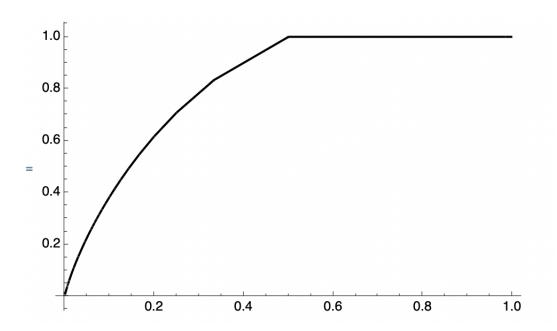
\includegraphics[width=0.7\textwidth]{assets/fig/_page_62_Figure_3.jpeg}
  \caption{$\log(L_{n,k})/n$ 作为 $\gamma = k/n$ 的函数在 $n \to \infty$ 时的边界.}\label{fig:5.0.3}
\end{figure}

\begin{proof}[引理~\ref{lem:5.0.1} 的证明]
我们从第~(1) 部分开始.
由素数定理, $[1, \ldots, n]$ 中的主要项(取对数后)由 $\sum_{p\le n} \log p$ 给出 (即我们只需计算素数而无需计算多重度).
这里的误差项与 $\gamma$ 无关.
因此 $[n - k, \dots, n]$ 的指数渐近速率是通过计算有多少个素数 $p \le n$ 整除 $n - k, \dots, n$ 中的至少一个来给出的.
在这一计数中唯一未出现的素数 $p \le n$ 是那些允许存在 $a \in \mathbf{N}_{>0}$ 使得 $ap < n - k$ 且 $(a + 1)p > n$ 的素数.
对于给定的 $a$, 所涉素数恰好是区间 $(n/(a + 1), (n - k)/a)$ 中的素数.
当且仅当 $a + 1 < 1/\gamma$ 时, 这是一个非空区间; 在这种情况下, 它的长度等于 $n((1 - \gamma)/a - 1/(a + 1))$.
因此, $\log [n - k, \dots, n]$ 等于
\[ n\left(1 - \sum_{a=1}^{\lfloor 1/\gamma \rfloor - 1} \left( \frac{1-\gamma}{a} - \frac{1}{a + 1} \right)\right) + o(n) \]
\[ = n\left(\gamma\left(\sum_{a=1}^{\lfloor 1/\gamma \rfloor - 1} 1/a\right) + 1/(\lfloor 1/\gamma \rfloor)\right) + o(n). \]

注意到根据我们的假设 $\gamma \geq \gamma_0$, 上述求和是一个项数具有一致上界的有限和.
此外, 来自素数定理的误差项得到了均匀控制, 因为它仅被应用于长度和端点在 $n$ 中得到一致控制的区间.

我们现在考虑引理~\ref{lem:5.0.1} 的情况~(2).
第一个断言的精确表述是: 对于任意 $\epsilon > 0$, 存在 $N = N(\epsilon)$ 和 $\delta = \delta(\epsilon)$ 使得对所有 $n > N$ 且 $k < \delta n$, 我们有 $\log L_{n,k} < \epsilon n$.
这是 (1) 的推论.
更确切地, 针对按定义有 $\delta < 1/2$, 对所有 $k < \delta n$, 我们有
\[ L_{n,k} \le L_{n,\delta n} = \exp\left(\left(\sum_{h=1}^{\lfloor 1/\delta \rfloor - 1} \frac{1}{h}\right) \delta n + \frac{n}{\lfloor 1/\delta \rfloor} + o_{\delta}(n)\right) \]
\[ \le \exp\left(\left(\delta(1 + \log(1/\delta)) + (1/\delta - 1)^{-1}\right) n + o_{\delta}(n)\right). \]

注意到 $\lim_{\delta\to 0} \left( \delta(1+\log(1/\delta)) + (1/\delta-1)^{-1} \right) = 0$; 我们选取一个 $\delta = \delta(\epsilon)$ 使得 $\delta(1+\log(1/\delta)) + (1/\delta-1)^{-1} < \epsilon/2$.
对于这个 $\delta$, 由 (1), 存在 $N = N(\delta,\epsilon) = N(\epsilon)$ 使得对 $n > N$, 误差项 $o_{\delta}(n) < (\epsilon/2)n$.
则对于所有 $n > N$ 且 $k < \delta n$, 我们有 $\log L_{n,k} < \epsilon n$.

第二个断言的精确表述是: 对于任意 $\epsilon > 0$, 存在 $N = N(\epsilon)$ 使得对所有 $n > N$ 且所有 $0 \le k \le n$, 我们有
\[ \log L_{n,k} \le \left(\sum_{h=1}^{\lfloor 1/\gamma \rfloor - 1} \frac{1}{h}\right) k + \frac{n}{\lfloor 1/\gamma \rfloor} + \epsilon n. \]

注意到由上述对第一个断言的证明, 存在 $\delta = \delta(\epsilon)$ 使得上述不等式对所有 $n > N_1(\epsilon)$ 且 $k < \delta n$ 成立.
此外, 根据第 (1) 部分取 $\gamma_0 = \delta$, 上述不等式对所有 $n > N_2(\delta, \epsilon) = N_2(\epsilon)$ 成立.
因此, 对于所有 $n > \max\{N_1(\epsilon), N_2(\epsilon)\}$, 所求边界成立.
\end{proof}

以下是上述引理的一个变体.

\begin{lemma}\label{lem:5.0.4}
\quad
\begin{enumerate}
  \item[(1)] 固定 $\gamma_0 \leq \gamma_0' \in (0,1)$. 对于满足 $\gamma_0 \leq k/n$ 且 $\gamma_0 \leq l/n \leq \gamma_0'$ 的 $k, l \leq n$, 大于 $l$ 且在区间 $[n-k, n]$ 内有倍数的素数 $p$ 的乘积 $L_{n,k}^{\geq l}$ 的对数, 在 $n \to \infty$ 时关于 $k, l$ 一致地渐近于
  \[ \left(k\sum_{h=1}^{\lfloor (n-k)/\max(k,l)\rfloor} 1/h\right) + \left(\frac{n}{\lfloor (n+(l-k)^+)/\max(k,l)\rfloor} - l\right)^+ + o(n), \]
  其中 $\alpha^+ := \max(0, \alpha)$, 且约定求和号 $\sum_{h=a}^b$ 遍历该范围内的所有整数, 若范围为空则求和为零.
  
  \item[(2)] 此外, 当 $n \to \infty$ 时, 对于所有 $0 \le k, l \le n$, 我们有
  \[ \log L_{n,k}^{\geq l} \le \left(k \sum_{h=1}^{\lfloor (n-k)/\max(k,l)\rfloor} 1/h\right) + \left(\frac{n}{\lfloor (n+(l-k)^+)/\max(k,l)\rfloor} - l\right)^+ + o(n), \]
  其中误差项关于所有 $k, l$ 是一致的. (若 $k = l = 0$, 则上式右端应理解为 $o(n)$.)
\end{enumerate}
\end{lemma}

\begin{proof}
我们从第 (1) 部分开始.
与引理~\ref{lem:5.0.1} 的证明类似, 在 $[n-k,\ldots,n]$ 中没有倍数的素数 $p \le n$ 是落在 $\bigcup_{a=1}^{\lfloor n/k\rfloor-1} (n/(a+1),(n-k)/a)$ 中的那些.
这里新增加的假设 $p > l$ 蕴含着 $a < (n-k)/l$, 从而
\[ \begin{split} 
& \left( \bigcup_{a=1}^{\lfloor (n-k)/k \rfloor} (n/(a+1), (n-k)/a) \right) \cap (l, n] \\ 
& = \left( \bigcup_{a=1}^{h_0-1} (n/(a+1), (n-k)/a) \right) \cup (\max(n/(h_0+1), l), (n-k)/h_0), 
\end{split} \]
其中 $h_0 = \lfloor (n - k)/\max(k, l) \rfloor$.

根据素数定理, 我们的渐近值由下式给出:
\[ n - l - \left(\sum_{a=1}^{h_0} ((n-k)/a - n/(a+1)) - (\max(n/(h_0+1), l) - n/(h_0+1))\right) + o(n) \]
\[ = k \left( \sum_{a=1}^{h_0} 1/a \right) + \max(n/(h_0 + 1), l) - l + o(n) = k \left( \sum_{a=1}^{h_0} 1/a \right) + (n/(h_0 + 1) - l)^+ + o(n), \]
且
\[ n/(h_0 + 1) = \frac{n}{\lfloor (n-k)/\max(k,l) \rfloor + 1} = \frac{n}{\lfloor (n+(l-k)^+)/\max(k,l) \rfloor}. \]

第二个断言 (2) 的精确表述是: 对于任何 $\epsilon > 0$, 存在 $N = N(\epsilon)$ 使得对所有 $n > N$ 且所有 $0 \le k, l \le n$, 我们有
\[ \log L_{n,k}^{\geq l} \le \left(k \sum_{h=1}^{\lfloor (n-k)/\max(k,l)\rfloor} 1/h\right) + \left(\frac{n}{\lfloor (n+(l-k)^+)/\max(k,l)\rfloor} - l\right)^+ + \epsilon n. \]

由引理~\ref{lem:5.0.1} (2), 存在 $\delta = \delta( \epsilon)$ 使得对于所有 $n > N_1(\epsilon)$ 和所有 $k \le \delta n$, 我们有
\[ \log L_{n,k}^{\geq l} \le \log L_{n,k} < \epsilon n. \]

因此, 我们现在假设 $k > \delta n$.
对于 $l < \min\{\delta, \epsilon/2\}n < k$, 由引理~\ref{lem:5.0.1} (1), 我们有对于 $n > N_2(\delta, \epsilon/2) = N_2(\epsilon)$,
\[ \log L_{n,k}^{\geq l} \le \log L_{n,k} \le \left(k \sum_{h=1}^{\lfloor (n-k)/k \rfloor} 1/h\right) + \frac{n}{\lfloor n/k \rfloor} + (\epsilon/2)n \]
\[ \le \left(k \sum_{h=1}^{\lfloor (n-k)/k \rfloor} 1/h\right) + \left(\frac{n}{\lfloor n/k \rfloor} - l\right)^{+} + \epsilon n, \]
这是所需的边界, 因为在此情况下 $\max(k,l)=k$.
对于 $l > (1-\delta/2)n$, 根据定义, 我们有 $\log L_{n,k}^{\geq l} \le \log L_{n,k}^{\geq (1-\delta/2)n}$.
将 (1) 应用于 $\gamma_0=\delta, \gamma_0'=1-\delta/2$, 存在 $N_3=N_3(\delta)=N_3(\epsilon)$ 使得对所有 $n > N_3$, 我们有
\[
\begin{aligned}
\log L_{n,k}^{\geq (1-\delta/2)n} 
&\le \left(k \sum_{h=1}^{\lfloor (n-k)/\max(k,(1-\delta/2)n)\rfloor} 1/h\right) \\
&\quad + \left(\frac{n}{\lfloor (n+((1-\delta/2)n-k)^+)/\max(k,(1-\delta/2)n)\rfloor} - (1-\delta/2)n\right)^+ + (\epsilon/2)n.
\end{aligned}
\]

注意到第一项为 $0$ (因为 $n-k < (1-\delta/2)n$), 且第二项 $\le n-((1-\delta/2)n \le (\delta/2)n$.
对于上述证明, 我们可以缩小 $\delta$ 使得 $\delta < \epsilon$, 从而以上讨论表明对于所有 $l \ge (1-\delta/2)n$, 我们有所需的边界
\[ \log L_{n,k}^{\geq l} \le \log L_{n,k} \le \epsilon n. \]

现在我们只需考虑 $k \ge \delta n$ 且 $\min\{\delta, \epsilon/2\}n \le l < (1 - \delta/2)n$, 此情况直接由 (1) 得出.
\end{proof}


% 引入第6节内容
\section{精细 holonomy 边界}\label{sec:6}

在本节中, 我们给出了第一个主要 holonomy 边界(定理~\ref{thm:6.0.2}), 我们通过重新审视 \cite[§ 2.5]{CDT21} 中的方法并利用 \S~3 和 \S~4 的(标准)结果对其进行增强来证明该定理.
这一对边界的初等处理对于定理~A 和 C 的证明以及我们在本文中的所有其他应用已经足够.
稍后, 在 \S~7 和 \S~8 中, 我们将证明其他 holonomy 边界, 其中一些涉及 Bost--Charles 双重积分, 该积分在理论上小于~\eqref{eq:6.0.15} 中的重排积分; 然而, 我们将在注记~8.1.17 和 \S~8.3 中发现, 这种差异在实践中微乎其微.
对于我们的默认处理, 我们选择突出递增重排特征, 在概率解释下, 该特征在 holonomy 商~\eqref{eq:6.0.10} 的顶端和底端数量中同时出现.

为了表述我们的 holonomy 边界, 我们首先(依据引理~\ref{lem:5.0.4})定义一个函数, 用于度量在将原始函数集的积分引入到多变量评估模中时, 对系数分母增加的额外贡献, 正如 \S~5 中所讨论的 (在定理~\ref{thm:6.0.2} 的表述中, 这些将是具有 $e_i > 0$ 的形式为~\eqref{eq:6.0.9} 的函数 $f_i$).

\begin{definition}\label{def:6.0.1}
对于 $0 \le \max\{u, 1\} \le v$ 且 $w \le v$, 设:
\[
\begin{aligned}
I_{u}^{v}(w) :=& \int_{\min\{u,1\}}^{1} \max\{t-w, 0\} dt + \int_{\max\{u,1\}}^{v} \left\{ \sum_{h=1}^{\lfloor \frac{t-1}{\max(1,w)} \rfloor} \frac{1}{h} \right\} dt \\
&+ \int_{\max\{u,1\}}^{v} \max\left\{ \frac{t}{\lfloor (t + \max(0, w - 1))/\max(1, w) \rfloor} - w, 0 \right\} dt.
\end{aligned}
\]
\end{definition}

我们现在有:

\begin{theorem}\label{thm:6.0.2}
考虑两个正整数 $m, r \in \mathbf{N}_{>0}$, 一个非负整数向量 $\mathbf{e} := (e_1, \dots, e_m) \in \mathbf{N}^m$, 以及一个 $m \times r$ 的非负实数矩形阵列:
\[ \mathbf{b} := (b_{i,j})_{1 \le i \le m, \ 1 \le j \le r}, \]
其所有列均具有如下形式:
\begin{equation}\label{eq:6.0.3}
0 = b_{1,j} = \dots = b_{u_j,j} < b_{u_j+1,j} = \dots = b_{m,j} =: b_j, \qquad \forall j = 1, \dots, r,
\end{equation}
其中 $u_j \in \{0, 1, \dots, m\}$ 取决于列.
设
\[ \sigma_i := b_{i,1} + \dots + b_{i,r}, \qquad i = 1, \dots, m \]
为第 $i$ 行的和, 并定义:
\begin{equation}\label{eq:6.0.4}
\tau^{\flat}(\mathbf{b}) := \frac{1}{m^2} \sum_{i=1}^{m} (2i - 1)\sigma_i = \sigma_m - \frac{1}{m^2} \sum_{j=1}^{r} u_j^2 b_j \in [0, \sigma_m],
\end{equation}
以及(其中 $I_{\xi}^m(\xi)$ 如定义~\ref{def:6.0.1} 所示):
\begin{equation}\label{eq:6.0.5}
\tau^{\sharp}(\mathbf{e}) := (2/m^2) \min_{\xi \in [0,m]} \left\{ \xi \sum_{i=1}^m e_i + \left( \max_{1 \le i \le m} e_i \right) I_{\xi}^m(\xi) \right\}.
\end{equation}
最后定义:
\begin{equation}\label{eq:6.0.6}
\tau(\mathbf{b}; \mathbf{e}) := \tau^{\flat}(\mathbf{b}) + \tau^{\sharp}(\mathbf{e}).
\end{equation}

考虑一族全纯映射 $\varphi_0, \dots, \varphi_l : (\overline{\mathbf{D}}, 0) \to (\mathbf{C}, 0)$, 其导数(共形半径)满足:
\begin{equation}\label{eq:6.0.7}
|\varphi_0'(0)| < |\varphi_1'(0)| < \dots < |\varphi_l'(0)| \quad 且 \quad |\varphi_l'(0)| > e^{\max(\sigma_m, \tau(\mathbf{b}; \mathbf{e}))}.
\end{equation}
相应地, 通过引入分割点参数来划分区间 $[0,m]$:
\[ 0 = \gamma_0 < \dots < \gamma_l < \gamma_{l+1} = m, \]
并利用这些选择, 通过在圆周 $\mathbf{T}$ 上根据 $[0,1)$ 到 $[\gamma_k/m, \gamma_{k+1}/m)$ 的线性缩放分段拼接函数 $\log |\varphi_k|$, 来定义一个 $L^1$ 函数:
\[ g_{\boldsymbol{\varphi},\boldsymbol{\gamma}}:[0,1)\to\mathbf{R}\cup\{-\infty\}, \]
\begin{equation}\label{eq:6.0.8}
g_{\boldsymbol{\varphi},\boldsymbol{\gamma}}(t):=\log\left|\varphi_k\left(e^{2\pi i\frac{mt-\gamma_k}{\gamma_{k+1}-\gamma_k}}\right)\right| \quad \text{当 } t\in[\gamma_k/m,\gamma_{k+1}/m).
\end{equation}

如果存在一个由 $m$ 个 $\mathbf{Q}(x)$-线性无关的形式幂级数组成的 $m$ 元组 $f_1, \dots, f_m \in \mathbf{Q}[\![x]\!]$, 其分母类型具有如下形式:
\begin{equation}\label{eq:6.0.9}
f_i(x) = a_{i,0} + \sum_{n=1}^{\infty} a_{i,n} \frac{x^n}{n^{e_i}[1, \dots, b_{i,1} \cdot n] \cdots [1, \dots, b_{i,r} \cdot n]}, \qquad a_{i,n} \in \mathbf{Z},
\end{equation}
使得对于所有对 $i = 1, \dots, m$ 和 $k = 0, \dots, l$, $f_i(\varphi_k(z)) \in \mathbf{C}[\![z]\!]$ 都是 $|z| < 1$ 上的亚纯函数芽, 那么:
\begin{align}
m &\le \frac{\int_{0}^{1} 2t \cdot g_{\boldsymbol{\varphi}, \boldsymbol{\gamma}}^{*}(t) dt + \frac{1}{m} \sum_{k=1}^{l} \gamma_{k}^{2} \log \frac{|\varphi_{k}'(0)|}{|\varphi_{k-1}'(0)|}}{\log |\varphi_{l}'(0)| - \tau(\mathbf{b}; \mathbf{e})} \nonumber\\
&= \frac{\int_{0}^{1} \int_{0}^{1} \max (g_{\boldsymbol{\varphi}, \boldsymbol{\gamma}}(s), g_{\boldsymbol{\varphi}, \boldsymbol{\gamma}}(t)) ds dt + \frac{1}{m} \sum_{k=1}^{l} \gamma_{k}^{2} \log \frac{|\varphi_{k}'(0)|}{|\varphi_{k-1}'(0)|}}{\log |\varphi_{l}'(0)| - \tau(\mathbf{b}; \mathbf{e})}.\label{eq:6.0.10}
\end{align}

如果此外所有函数 $f_i$ 都被先验地假定为 holonomic, 则在方程~\eqref{eq:6.0.7} 中对 $\varphi_l$ 的假设 $|\varphi'_l(0)| > e^{\max(\sigma_m, \tau(\mathbf{b}; \mathbf{e}))}$ 可以放宽为 $|\varphi'_l(0)| > e^{\tau(\mathbf{b}; \mathbf{e})}$.
\end{theorem}

这里, 在 $g^*$ 中我们使用了~\eqref{eq:2.4.1} 中 $g$ 的递增重排函数的记号.
这就是为什么我们经常将诸如 $\int_0^1 2t \cdot g^*(t) dt = \iint_{[0,1]^2} \max(g(s), g(t)) ds dt$ 之类的量称为重排积分 (rearrangement integrals).

\begin{remark}[音乐记号]\label{rem:6.0.11}
在定理~\ref{thm:2.5.1} 的记号中, 我们有 $\tau(\mathbf{b}) = \tau^{\flat}(\mathbf{b}) = \tau(\mathbf{b}; \mathbf{0})$.
我们使用这种音乐记号的原因是将 $\tau = \tau^{\flat}(\mathbf{b})$ 视为去除~\eqref{eq:7.0.1} 中幂次 $n^{\mathbf{e}}$ 时, 对来自 \cite{CDT24} 的较粗糙值 $\tau = \sigma_m$ 的主规约(降音/flattening), 并将 $\tau^{\sharp}(\mathbf{e})$ 视为在原始函数列表中加入这些积分所带来的额外项(升音/sharpening).
\end{remark}

\begin{remark}\label{rem:6.0.12}
在定理~\ref{thm:6.0.2} (以及我们证明的所有其他类似定理)中, 我们实际上可以放宽分母类型~\eqref{eq:6.0.9}, 允许具有如下更宽松的形式:
\begin{equation}\label{eq:6.0.13}
n^{e_i}[1, \dots, b_{i,1} \cdot n + c_{i,1}] \cdots [1, \dots, b_{i,r} \cdot n + c_{i,r}],
\end{equation}
其中 $c_{i,j}$ 为任意给定的整数集.
这可以通过应用我们定理的原始陈述得到, 其中所有非零的 $b_{i,j}$ 都替换为 $b_{i,j} + \varepsilon$ (对于某个足够小的正数 $\varepsilon > 0$).
这对于除有限多个 $n$ 之外的所有情况都包含了分母类型~\eqref{eq:6.0.13}, 并且任何有限的系数初始段都可以通过缩放使其具有任何给定的分母类型.
然后, 注意到这些边界总是连续地依赖于 $b_{i,j}$, 取极限 $\varepsilon \to 0$ 即可.
\end{remark}

作为单个解析映射 $\varphi$ 的特殊情况 $l=0$, 我们记录边界~\eqref{eq:2.5.5} 的推广:

\begin{corollary}\label{cor:6.0.14}
假设与定理~\ref{thm:6.0.2} 相同的条件和记号, 但更简单地考虑单个全纯映射 $\varphi: (\overline{\mathbf{D}}, 0) \to (\mathbf{C}, 0)$, 其满足 $|\varphi'(0)| > e^{\tau(\mathbf{b}; \mathbf{e})}$, 且使得拉回 $\varphi^* f_i$ 在开单位圆盘上是亚纯函数, 即 $\varphi^* f_i \in \mathcal{M}(\mathbf{D})$.
如果要么 $|\varphi'(0)| > e^{\sigma_m}$, 要么所有函数 $f_i$ 都是 holonomic, 那么:
\begin{equation}\label{eq:6.0.15}
m \le \frac{\iint_{\mathbf{T}^2} \log \left( \max(|\varphi(z)|, |\varphi(w)|) \right) \mu_{\mathrm{Haar}}(z) \mu_{\mathrm{Haar}}(w)}{\log |\varphi'(0)| - \tau(\mathbf{b}; \mathbf{e})} = \frac{\int_0^1 2t \cdot (\log |\varphi(e^{2\pi it})|)^* dt}{\log |\varphi'(0)| - \tau(\mathbf{b}; \mathbf{e})}.
\end{equation}
\end{corollary}

\begin{remark}\label{rem:6.0.16}
如果我们仅假设 $|\varphi'(0)| > e^{\tau(\mathbf{b};\mathbf{e})}$, 则先验的 holonomic 性质是不能丢弃的.
更确切地说, 对于在比例~\ref{cor:6.0.14} 的陈述中的任何给定的数据组 $(\mathbf{b};\varphi)$, 如果假设相反的不等式 $|\varphi'(0)| \le e^{\sigma_m}$, 那么一个简单的归纳构造就可以说明如下结论: 如果存在至少一个满足该数据组 $(\mathbf{b};\varphi)$ 的算术和解析条件的 $\mathbf{Q}(x)$-线性无关的形式函数 $m$ 元组 $\{f_i\}$, 那么就存在连续统(continuum)个这样的 $m$ 元组; 这尤其意味着存在非 holonomic 的此类函数.

为了说明这一断言, 在固定 $f_1, \ldots, f_{m-1}$ 的情况下, 证明对于在 $e_m = 0$ 的形式~\eqref{eq:6.0.9} 下的 $f_m \in \mathbf{Q}[\![x]\!]$, 存在连续统个有效的系数选择 $a_{m,\bullet} \in \mathbf{Z}$, 使得拉回幂级数 $\sum c_n z^n := f_m(\varphi(z)) \in \mathbf{C}[\![z]\!]$ 具有次指数级小的系数 $|c_n| = \exp(o(n))$ 就足够了 (对比 \cite[§ 6.4.2]{BC22}, \cite[§ 6]{Pol1923} 或 \cite[§ 5]{Rob68}).
我们展示出在所有先前的系数 $a_{m,0}, \ldots, a_{m,n-1}$ 已经被选择好之后, 每个后续系数 $a_{m,n} \in \mathbf{Z}$ 具有至少两个有效的选项.
这通过递归地将 $c_n = \mu_n a_{m,n} - P_n(a_{m,0}, \ldots, a_{m,n-1})$ 表达出来而得到, 其中系数
\[ \mu_n := \varphi'(0)^n / \prod_{i=1}^h [1, \dots, b_{m,i} \cdot n] \]
通过素数定理具有次指数级增长, 且 $P_n \in \mathbf{C}[x_0, \dots, x_{n-1}]$ 是取决于映射 $\varphi$ 的多项式.
这给出了两个不同的有效选项 $a_{m,n} \in \{\lfloor P_n(\mathbf{a}_{m,< n})/\mu_n \rfloor, \lfloor P_n(\mathbf{a}_{m,< n})/\mu_n \rfloor + 1\}$, 并由此构造了一个基数为 $2^{\#\mathbf{N}} = \#\mathbf{R}$ 的 $f_m \in \mathbf{Q}[\![x]\!]$ 集合.
\end{remark}

本节中一个至关重要的技术特征, 并最终用于定理~A 和 C 的证明, 是容纳增加积分的项 $\tau^{\sharp}$, 它补充了定理~2.5.1 的主要分母形式.
我们通过几个例子来描述这一特征.

\begin{remark}[基本注记 6.0.17]\label{rem:6.0.17}
重新审视来自基本注记~2.6.3 的最简单的例子, 让我们计算如下情况下的 $\tau(\mathbf{b}; \mathbf{e})$:
\[ \mathbf{b} = (0,0)^{\mathrm{t}}, \quad \mathbf{e} = (0,1). \]
显然 $\tau^{\flat}(\mathbf{b}) = 0$, 并且我们很容易计算出:
\[ \tau^{\sharp}(\mathbf{e}) = \frac{1}{2} \min_{\xi \in [0,2]} \left\{ \frac{3 + (\xi - 1)^2}{2} \right\} = \frac{3}{4}, \]
这在终点 $\xi = 1$ 处达到.
因此我们发现了与采用较粗糙方案时相同的数值 $\tau(\mathbf{b}, \mathbf{e}) = \tau^{\flat}(\mathbf{b}) + \tau^{\sharp}(\mathbf{e}) = 3/4$:
\[
\begin{aligned}
\mathbf{b} &= (0, 1)^t, \qquad \mathbf{e} = (0, 0), \\
\tau^{\flat}(\mathbf{b}) &= 3/4, \quad \tau^{\sharp}(\mathbf{e}) = 0,
\end{aligned}
\]
在此例中与 \S~2.5 相比并没有取得改进.

稍后, 我们将重新审视并改进 \cite[§ 2.1]{CDT21} 中的丢番图逼近框架.
在关于我们运行的例子的那个框架中, 我们有如下形式的辅助函数(复制到许多变量): $P(x) + Q(x) \log(1-x)$, 其中 $P, Q \in \mathbf{Z}[x]$ 是次数小于 $D$ 的多项式.
根据 \S~3.3.7 中的讨论, 任何此类函数的最低阶单项式 $\beta x^n$ 的次数必然满足 $n \le 2D - 1$, 其中等号由 Hermite--Pad{\'e} 逼近式(本质上由 Legendre 多项式给出)唯一达到.
我们的证明方案结合了对系数 $\beta \in \mathbf{Q}^{\times}$ 的解析上界与通过非零有理数 $\beta$ 分母的倒数给出的算术下界 $|\beta| > 1/\text{den}(\beta)$.
我们可以直接看出为什么在这种情况下, $\log(1-x) = -\sum_{k=1}^{\infty} x^k/k$ 的更精细分母并没有给算术下界 $|\beta| \ge 1/\text{den}(\beta)$ 带来任何额外帮助.
$x^n$ 系数 $\beta \in \mathbf{Q}$ 的分母是通过区间 $[n-D, n] \supset [n/2, n]$ 中所有整数的最小公倍数来估计的.
因为 $[n/2, \dots, n] = [1, \dots, n]$ (对于每个整数 $k \in [1, n]$, 都存在唯一的 $2$ 的幂次倍数落在 $(n/2, n]$ 内), 在这种情况下, 这等于整个初始整数组的最小公倍数 $[1, \dots, n]$: 这正是我们通过在函数 $f(x) = \log(1-x)$ 中用 $[1, \dots, k]$ 代替 $k$ 作为系数分母所得到的估计.
我们还看到, 一旦我们有至少 $m \ge 3$ 个函数, 预计更精细的分母就会产生影响, 因为 $[2n/3, \dots, n]$ 已经显著小于 $[1, \dots, n]$ (参见基本注记~5.0.2). \end{remark}

\begin{remark}\label{rem:6.0.18}
利用精细的对 $\mathbf{b} \in M_{m \times r}(\mathbf{N})$ 与 $\mathbf{e} \in \mathbf{N}^m$, 而不是粗糙地拼接成 $\mathbf{e} \leadsto \mathbf{0}$, 并不总是能对定理~\ref{thm:6.0.2} 的估计给出改进.
考虑 $m=3$ 且处于定理~2.7.2 证明的情况, 但具有更精细的类型:
\[ \mathbf{b} = (0, 0, 1)^{\mathrm{t}}, \quad \mathbf{e} = (0, 1, 0), \]
这给出了一个包含三个具有如下分母类型函数的模板:
\begin{equation}\label{eq:6.0.19}
x^n, \ \frac{x^n}{n}, \ \frac{x^n}{[1, \dots, n]}.
\end{equation}
这一对阵列 $(\mathbf{b}; \mathbf{e})$ 的选择具有 $\tau^{\flat}(\mathbf{b}) = \tau^{\sharp}(\mathbf{e}) = 5/9$, 后者在整个区间 $\xi \in [3/2, 2]$ 上达到最小值.
但是类型~\eqref{eq:6.0.19} 也被我们在定理~2.7.2 的证明中所作的更粗糙的选择所包含:
\[ \mathbf{b}_0 := (0, 1, 1)^{\mathbf{t}}, \quad \mathbf{e}_0 = (0, 0, 0), \]
并且在这一情况下, 这一基本选择给出了更好的数值 $\tau(\mathbf{b}_0; \mathbf{e}_0) = \tau(\mathbf{b}_0) = 8/9$, 而不是 $\tau(\mathbf{b}; \mathbf{e}) = 10/9$.
原因在于在定理~\ref{thm:6.0.2} 的证明中, 辅助函数首项系数的分母是如何被估计的; 速率 $\tau^{\flat}(\mathbf{b}) + \tau^{\sharp}(\mathbf{e})$ 作为一个上界, 而在目前的例子中, 该上界估计被证明是严格且有损失的.
我们不知道在最终用于证明定理~A 的 $m = 14$ 的情况下该上界是否为等式, 但我们预计它是一个相当精确的分母估计, 甚至可能是等式. \end{remark}

\begin{example}\label{exa:6.0.20}
我们给出最后一个例子, 我们将在 \S~6.8 中使用它来完成定理~2.8.4 的证明.
对于适用于具有如下分母类型的四个函数集合的矩阵:
\[ \mathbf{b} = \begin{pmatrix} 0 & 0 \\ 0 & 2 \\ 0 & 2 \\ 1 & 2 \end{pmatrix}, \qquad \mathbf{e} = (0, 0, 1, 0) \]
这些类型为:
\begin{equation}\label{eq:6.0.21}
x^n, \quad \frac{x^n}{[1,\dots,2n]}, \quad \frac{x^n}{n[1,\dots,2n]}, \quad \frac{x^n}{[1,\dots,n][1,\dots,2n]},
\end{equation}
我们有:
\[ \tau^{\flat}(\mathbf{b}) = \frac{37}{16}, \quad \tau^{\sharp}(\mathbf{e}) = \frac{7}{16}, \qquad \tau(\mathbf{b}; \mathbf{e}) = \frac{21}{8} = 2.625, \]
其中 $7/16$ 的值在相同的区间极小值 $\xi \in [2, 3]$ 上达到.
但是, 即使是微弱地包含了引言中所强调的定理~2.5.1 框架内的类型~\eqref{eq:6.0.21} 的中间粗糙选择:
\[ \mathbf{b}_0 = \begin{pmatrix} 0 & 0 \\ 0 & 2 \\ 1 & 2 \\ 1 & 2 \end{pmatrix}, \qquad \mathbf{e}_0 = (0, 0, 0, 0), \]
也已经给出了:
\[ \tau(\mathbf{b}_0; \mathbf{e}_0) = \tau(\mathbf{b}_0) = \frac{1}{16} (1 \cdot 0 + 3 \cdot 2 + 5 \cdot 3 + 7 \cdot 3) = \frac{21}{8} = 2.625. \]
在这一情况下, 数值是相同的, 类似于基本注记~6.0.17 中的情形. \end{example}

与上述例子形成对比的是, 利用精细化对 $(\mathbf{b}; \mathbf{e})$ 往往确实能产生严格优于通过对某些粗糙的 $\mathbf{e} \leadsto \mathbf{0}$ 方案进行封顶所能达到的结果.
对于在 \S~13 中给出的定理~A 的证明来说尤其如此.
在那里, 我们有一个阶为 $m = 14$ 的包含增加积分的局部系统, 意味着对于其中六个指数有 $e_i = 1$, 而对于其余八个指数有 $e_i = 0$.
经过简单的计算~\eqref{eq:13.0.5}, 这样的向量具有 $\tau^{\sharp}(\mathbf{e}) = 27/80$.
整体上, 所使用的精细 $\tau(\mathbf{b}; \mathbf{e})$ 计算出为 $191/49 + 27/80 = 16603/3920 = 4.235459 \dots$.
但在该例子中, 使用 $\mathbf{e} = \mathbf{0}$ 类型无法得到优于注记~13.0.7 中相当差的 $865/196 = 4.413265 \dots$ 的估计.

\subsection{水平积分}\label{sec:6.1}
\setcounter{footnote}{19}

我们的证明方案精确地遵循了我们起初为关于无界分母猜想的首个解答 \cite[§ 2.5]{CDT21} 所设计的 $d \to \infty$ 渐近方法.
这就是我们所谓的``跨变量积分''的想法, 其中给定的单变量函数 $f_i(x)$ 在 $d \to \infty$ 的分裂变量中被复制, 以便利用 Dirichlet 抽屉原理构造一个非零辅助函数:
\begin{equation}\label{eq:6.1.1}
F(x_1, \dots, x_d) := \sum_{\substack{\mathbf{i} \in \{1, \dots, m\}^d \\ \mathbf{k} \in [0, D]^d \cap \mathbf{Z}^d}} c_{\mathbf{i}, \mathbf{k}} x_1^{k_1} \cdots x_d^{k_d} f_{i_1}(x_1) \cdots f_{i_d}(x_d) \in \mathbf{Q}[[x_1, \dots, x_d]] \setminus \{0\},
\end{equation}
其具有次指数级渐近大小的整数系数 $c_{\mathbf{i},\mathbf{k}} \in \mathbf{Z}$:
\[ |c_{\mathbf{i},\mathbf{k}}| = \exp\left(o_{d\to\infty}(dD)\right), \]
但 $F(x_1, \ldots, x_d)$ 却在 $\mathbf{x} = \mathbf{0}$ 处消亡至几乎最高可想象的阶 $\alpha$.
奇妙的是, 在这个方案中, Nevanlinna 特征增长项 $\int_{\mathbf{T}} \log^+ |\varphi| \, \mu_{\text{Haar}}$ 并非作为圆周积分本身出现 (外加可能无论是通过 \cite[§ 2.3 或 § 2.4]{CDT21}, 还是通过我们在下面 \S~7 中基于 \cite{BC22} 和 \cite{CDT24} 的讨论); 而是通过标准的大偏差边界\footnote{这只是我们在 \S~4 中详细讨论的定理~\ref{thm:4.2.1} 的重述. 事实上, 指数函数建立了测度空间 ($[0,1]^d$, $\mu_{\text{Lebesgue}}$) 和 ($\mathbf{T}^d$, $\mu_{\text{Haar}}$) 之间的同构, 在该同构下方体偏差函数相对应.}——其要求一旦 $d \ge d_0(\epsilon)$, 高维环面 $\mathbf{T}^d$ 上的低偏差集合 $D(\mathbf{z}) < \epsilon$ 具有至少 $1 - Ce^{-c\epsilon^4 d}$ 的测度——从拉回单项式 $\varphi(z_1)^{k_1} \cdots \varphi(z_d)^{k_d}$ 的优势增长率中产生.
这就是为什么我们会把这种方法描述为以跨变量的方式进行积分, 或者如果将丢番图逼近构造中维度、次数和 $\mathbf{T}$ (任意一个固定变量中的复分析)等各个方面可视化, 则称为``水平地''进行积分.

本论文的主要发现之一是 \S~3 和 \S~4 的某种结合, 它实际上改进了~\eqref{eq:6.1.1} 中``最高可想象消亡阶'' $\alpha$ 的含义.
在 \cite[§ 2]{CDT21} 较粗糙的处理中, 在待求未知数 $c_{i,k}$ 的线性方程组个数的参数计数中, 我们仅有 $\alpha = mdD/e - o_{d\to\infty}(dD)$; 这归因于标准高维单纯形与其最大嵌入子立方体的 $e^d:1$ 渐近体积比.
我们现在解释关于与 Cartesian 乘积的消亡过滤跳跃集合形成的可交换性的推论~\ref{cor:3.1.11}, 以及测度集中材料 \S~4 如何协同工作以将该消亡阶改进为 $\alpha = mdD/2 - o_{d\to\infty}(dD)$.
为了简单起见, 因为我们稍后在定理~\ref{thm:6.0.2} 的一般形式中无论如何都会需要它, 我们假设基于 $f_i$ 的 holonomic 性质的最强形式的 Cartesian 幂结构: 引理~\ref{lem:3.2.14}, 它源于 Chudnovsky--Osgood 定理与推论~\ref{cor:3.1.11} 的结合.

\subsubsection{Thue--Shidlovsky 思想}\label{sec:6.1.2}

引理~\ref{lem:3.2.14} 确保了一旦 $D \gg_{\delta,d} 1$, 非零幂级数~\eqref{eq:6.1.1} 对于任何 $\delta > 0$ 和 $d$, 必须拥有一个具有非零单项式 $\beta \mathbf{x}^{\mathbf{n}} = \beta x_1^{n_1} \cdots x_d^{n_d}$ 且 $\mathbf{n} = (n_1, \dots, n_d) \in [0, (m+\delta)D]^d$ 的项.
因此, 在 Thue--Siegel 引理中用于求解总消亡阶的线性方程组中, 我们不需要关心宽单纯形区域 $|\mathbf{n}| < \alpha$, 而是可以简单地使 $\mathbf{x}^{\mathbf{n}}$ 的系数在遍历超立方体 $[0, (m-\delta)D]^d$ 的所有 $\mathbf{n}$ 时消亡 (显然, 这是参数计数中最大可想象的超立方体), 以及在稍大超立方体 $[0, (m+\delta)D]^d$ 的低偏差部分之外的所有 $\mathbf{n}$ 处消亡 (允许我们对向量 $\mathbf{n}$ 的分量集合也使用测度集中).
这里为了应用定理~\ref{thm:4.2.1}, 根据偏差参数 $\epsilon$ 选取足够小的 $\delta > 0$ 是至关重要的; 然后参数计数就能顺利通过 (这一步包含在引理~\ref{lem:6.2.6} 中).
其结果是在该构造中, 随着 $\epsilon \to 0$ (最终在 $D \to \infty, d \to \infty, \delta \to 0$ 之后), $F(x_1,\ldots,x_d)$ 中所有最低阶单项式 $\beta \cdot x_1^{n_1} \cdots x_d^{n_d}$ 的指数向量 $(n_1,\ldots,n_d)$ 渐近地接近于集合 $\{jmD/d: 0 \le j < d\}$ 的某种排序.
特别是, 总消亡阶确实接近于 $mdD/2$.

正是这种相比于 \cite[Lemma 2.1.2]{CDT21} 的 $mdD/e$ 的改进, 在 \cite[§ 2]{CDT21} 的初等渐近框架下恢复了 $e \rightsquigarrow 2$ 的系数改进.
在这一点上, Thue--Shidlovsky 论证进一步对分式~\eqref{eq:2.2.3} 的顶端和底端提供了两个类似且同样关键的改进.

接下来我们依次引入这两个改进, 为简单起见以推论~\ref{cor:6.0.14} 的情况为例, 随后我们开始定理~\ref{thm:6.0.2} 的一般证明.

\subsubsection{阿基米德精细化}\label{sec:6.1.3}

首先, 这一渐近方案允许通过初等方法将积分 $\int_{\mathbf{T}} \log^+ |\varphi| \, \mu_{\text{Haar}}$ 改进为严格较小的量 $\int_0^1 t \cdot (\log |\varphi(e^{2\pi it})|)^* \, dt$.
我们已经在 \cite[§ 2.3.3]{CDT21} 中指出, 通过再次利用定理~\ref{thm:4.2.1}, 可以将~\eqref{eq:6.1.1} 中的单项式指数 $\mathbf{k}$ 限制在超立方体 $[0,D]^d$ 的低偏差部分, 从而实现对 holonomy 边界的一些改进.
用具体的启发式语言来说, 这意味着当 $d \to \infty$ 时, 指数向量 $(k_1,\ldots,k_d)$ 在~\eqref{eq:6.1.1} 中可以被认为接近于集合 $\{jD/d:0\le j< d\}$ 的某种排序.
通过这种方式, 注意到在所有这些排序中, $|\varphi(z_1)^{k_1}\cdots\varphi(z_d)^{k_d}|$ 的最大值发生在 $(k_1,\ldots,k_d)$ 与 $(|\varphi(z_1)|,\ldots,|\varphi(z_d)|)$ 具有相同排列顺序的时候, 我们发现重排积分:
\begin{equation}\label{eq:6.1.4}
\int_{0}^{1} t (\log |\varphi|)^{*}(t) dt = \frac{1}{2} \iint_{\mathbf{T}^{2}} \log (\max(|\varphi(z)|, |\varphi(w)|)) \ \mu_{\text{Haar}}(z) \mu_{\text{Haar}}(w)
\end{equation}
恰好在基于不仅环面点 $\mathbf{z} \in \mathbf{T}^d$ 的均匀分布, 而且单项式指数向量 $\mathbf{k}$ 的均匀分布的精细优势增长率中出现.
图~8.1.15 的显式例子展示了这样所节省的幅度.

\subsubsection{算术精细化}\label{sec:6.1.5}

对于 $F(x_1,\ldots,x_d)$ 的首项射流指数 $\mathbf{n}$ 的均匀分布, 我们还可以加入大数定律的另一个初等应用: 在不改变(广义上)参数计数渐近大小的情况下, 我们可以坚持要求 $m$ 个函数种类在组成~\eqref{eq:6.1.1} 的所有分裂变量乘积 $f_{i_1}(x_1)\cdots f_{i_d}(x_d)$ 中以相等的频率 $1/m$ 出现.
换句话说, 我们可以假设 $d \equiv 0 \mod m$, 并且求和多重指数 $\mathbf{i}$ 在~\eqref{eq:6.1.1} 中被限制为每个指数 $i_0 \in \{1,\ldots,m\}$ 作为 $\mathbf{i}$ 的分量出现 $d/m$ 次.
这允许我们对我们 $m$ 个函数种类的 $m$ 个不同分母类型进行求和, 在我们对分母上限阵列 $\mathbf{b}$ 的条件下, 我们恰好发现~\eqref{eq:2.5.6} 作为~\eqref{eq:2.4.2} 的对应物.

\subsection{辅助构造}\label{sec:6.2}

我们在此开始定理~\ref{thm:6.0.2} 的证明.
在所有 $f_i$ 都被先验地假定为 holonomic 函数的情况下, 我们对 \cite[Lemma 2.1.2]{CDT21} 具有如下改进.

对于 $d \in \mathbf{N}_{>0}$ 且 $\epsilon \in (0,1]$, 我们用
\begin{equation}\label{eq:6.2.1}
P_{\epsilon}^{d} := \{ \mathbf{t} \in [0,1]^{d} : D(\mathbf{t}) < \epsilon \} \subset [0,1]^{d}
\end{equation}
表示 $d$ 维超立方体的 $\epsilon$-偏差部分, 其中 $D:[0,1]^d \to [0,1]$ 是定义~\ref{def:4.1.1} 的归一化偏差函数.
该集合在解析同构 $\exp:[0,1)^d \to \mathbf{T}^d$, $\mathbf{t} \mapsto e^{2\pi i \mathbf{t}}$ 下的像将记为 $T^d_\epsilon \subset \mathbf{T}^d$.
在这些记号中, 定理~\ref{thm:4.2.1} 的较粗糙形式可以重述为如下双重极限:
\begin{equation}\label{eq:6.2.2}
\lim_{\varepsilon \to 0} \lim_{d \to \infty} \mu_{\text{Lebesgue}}(P_{\varepsilon}^{d}) = 1, \qquad \lim_{\varepsilon \to 0} \lim_{d \to \infty} \mu_{\text{Haar}}(T_{\varepsilon}^{d}) = 1.
\end{equation}

在下文中, 我们固定一个 $m \in \mathbf{N}_{_{>0}}$, 并将渐近参数 $d \in \mathbf{N}_{>0}$ 限制为满足 $d \equiv 0 \mod m$ 的整数.
为了执行 \S~6.1.5 中概述的方案, 我们将~\eqref{eq:6.1.1} 中的多重指数 $\mathbf{i}$ 限制在如下等分布集合中:
\begin{equation}\label{eq:6.2.3}
V_m^d := \{ \mathbf{i} : \forall i \in \{1, \dots, m\}, \#\{h \in \{1, \dots, d\} : i_h = i\} = d/m \} \subset \{1, \dots, m\}^d.
\end{equation}
该集合仍然具有渐近满大小 $m^{d-o(d)}$:

\begin{lemma}\label{lem:6.2.4}
在我们立论的假设 $d \equiv 0 \mod m$ 下, 我们有:
\begin{equation}\label{eq:6.2.5}
\#V_m^d = {d \choose \frac{d}{m}, \dots, \frac{d}{m}} > m^d / {d+m-1 \choose m-1}.
\end{equation}
\end{lemma}

\begin{proof}
$m$-fold 展开式
\[ m^{d} = (1 + \dots + 1)^{d} = \sum_{\substack{\mathbf{j} \in \mathbf{N}^{m} \\ |\mathbf{j}| = d}} {d \choose j_{1}, \dots, j_{m}} \]
具有 $\binom{d+m-1}{m-1}$ 项, 其中最大的一项是具有 $j_1=\dots=j_m=d/m$ 的中心多项式系数.
\end{proof}

我们的 Thue--Siegel 构造(来自 \S~2.12 中一般大纲的步骤 (ii))如下.

\begin{lemma}\label{lem:6.2.6}
假设我们有 $m$ 个 holonomic 形式幂级数 $f_1, \ldots, f_m \in \mathbf{Q}[\![x]\!]$.
假定每个 $f_i(x)$ 具有如下粗糙类型的分母:
\begin{equation}\label{eq:6.2.7}
f_i(x) = \sum_{n=0}^{\infty} a_{i,n} \frac{x^n}{A^{n+1}[1,\dots,Bn]^{\sigma}}, \quad \text{其中 } A \in \mathbf{N}_{>0}, \ B, \sigma \in \mathbf{N}
\end{equation}
且在复圆盘 $|x| < \rho$ 上收敛, 对于某个 $\rho \in (0,1)$.

存在一个函数
\[ d_0: \mathbf{N}^3 \times (0,1) \times (0,1) \to \mathbf{N} \]
使得如下结论成立.

对于每个 $\epsilon \in (0,1)$, 存在一个 $\delta = \delta(\epsilon) \in (0,\epsilon)$, 使得对所有满足 $d \geq d_0(A,B,\sigma,\rho;\epsilon)$ 且 $d \equiv 0 \mod m$ 的 $d$, 当 $D \to \infty$ 时, 渐近地存在一个形如~\eqref{eq:6.1.1} 的非零 $d$ 元形式函数 $F(\mathbf{x})$:
\begin{equation}\label{eq:6.2.8}
F(\mathbf{x}) = \sum_{\substack{\mathbf{i} \in V_m^d \\ \mathbf{k}/D \in P_{\epsilon}^d \cap \mathbf{Z}^d}} c_{\mathbf{i}, \mathbf{k}} \mathbf{x}^{\mathbf{k}} \prod_{s=1}^d f_{i_s}(x_s) \in \mathbf{Q}[\![\mathbf{x}]\!] \setminus \{0\},
\end{equation}
其具有整数系数 $c_{\mathbf{i},\mathbf{k}} \in \mathbf{Z}$, 绝对值均由 $|c_{\mathbf{i},\mathbf{k}}| < e^{\epsilon dD}$ 控制, 且使得~\eqref{eq:6.2.8} 的幂级数展开 $F(\mathbf{x}) = \sum b_{\mathbf{n}} \mathbf{x}^{\mathbf{n}}$ 满足如下主要要求:
\begin{equation}\label{eq:6.2.9}
\begin{gathered}
\star \quad \text{\autoref{eq:6.2.8} 中的所有极小阶单项式 $\beta_{\mathbf{n}} \mathbf{x}^{\mathbf{n}}$，} \\
\text{其指数向量 $\mathbf{n}$ 均满足 $\mathbf{n}/((m+\delta)D) \in P_e^d$。}
\end{gathered}
\end{equation}
\end{lemma}

注意到 $(\star)$ 尤其意味着在集合 $((m+\delta)D) P_{\epsilon}^d \cap \mathbf{Z}^d$ 中, 至少存在一个这样的 $\mathbf{n}$ 使得 $\beta_{\mathbf{n}} \neq 0$.

在进行证明之前, 我们收集一些由条件 $(\star)$ 带来的推论.
在下文中, 我们将考虑最终让其趋近于零的 $\epsilon \in (0,1/4]$.
在整个 \S~6 中, 我们将写入:
\begin{equation}\label{eq:6.2.10}
\alpha := mdD/2.
\end{equation}
该记记号反映了 $\alpha$ 作为消亡参数在 \cite[§ 2]{CDT21} 中的相关使用, 见例如 \cite[Lemma 2.1.2(1)]{CDT21}.
在先前的论文中, 我们(在渐近意义上)取 $\alpha$ 为(阶数在) $mdD/e \sim m(d!)^{1/d}D$, 我们在此处将其改进为 $mdD/2$.

\begin{corollary}\label{cor:6.2.11}
在引理~\ref{lem:6.2.6} 中, 我们有:
\begin{equation}\label{eq:6.2.12}
\operatorname{ord}_{\mathbf{x}=\mathbf{0}} F(\mathbf{x}) \in [(1-2\epsilon)\alpha, (1+2\epsilon)^2 \alpha].
\end{equation}
每个~\eqref{eq:6.2.8} 中的多重指数 $\mathbf{k} = (k_1, \dots, k_d)$ 均满足 $\max_{j=1}^d k_j \leq \frac{2\alpha}{md}$, 并且允许 $\{1, \dots, d\}$ 的一个置换 $\psi = \psi_{\mathbf{k}}$ 使得 $k_{\psi(1)} \leq \dots \leq k_{\psi(d)}$ 且有:
\begin{equation}\label{eq:6.2.13}
\frac{2\alpha j}{md^2} - 2\epsilon \alpha/(md) \le k_{\psi(j)} \le (1+\epsilon) \frac{2\alpha j}{md^2} + 4\epsilon \alpha/(md), \qquad \forall j \in \{1, \dots, d\}.
\end{equation}
此外, Taylor 级数 $F(\mathbf{x}) \in \mathbf{Q}[\![\mathbf{x}]\!]$ 中具有最低总阶数 $n := |\mathbf{n}| = \operatorname{ord}_{\mathbf{x} = \mathbf{0}} F(\mathbf{x})$ 的每个指数 $\mathbf{n} = (n_1, \dots, n_d)$ 都具有 $\{1,\ldots,d\}$ 的一个置换 $\pi$ 使得 $n_{\pi(1)} \leq \dots \leq n_{\pi(d)}$ 且:
\begin{equation}\label{eq:6.2.14}
2\alpha j/d^2 - 2\epsilon \alpha/d \le n_{\pi(j)} \le (1+\epsilon)2\alpha j/d^2 + 4\epsilon \alpha/d, \qquad \forall j \in \{1, \dots, d\},
\end{equation}
且对所有满足 $u \leq v$ 的 $u, v \in [0, 1]$, 它都满足:
\begin{equation}\label{eq:6.2.15}
(1 - 2\epsilon)(v^2 - u^2)\alpha \le \sum_{ud \le j < vd} n_{\pi(j)} \le (1 + 2\epsilon)^2 (v^2 - u^2)\alpha.
\end{equation}
\end{corollary}

\begin{proof}
偏次数边界~\eqref{eq:6.2.13} 只是我们定义~\eqref{eq:6.2.10} 的重写, 但它被用于将分析组织在首项渐近参数 $\alpha$ 周围.
估计式~\eqref{eq:6.2.12} 随后由下式得出, 其中注意到期望值 $\mathbf{E}\left[t\in[0,1]\right]=\int_0^1t\,dt=1/2$, 这由 Koksma--Hlawka 不等式或初等的计算显示出如下蕴含关系:
\begin{equation}\label{eq:6.2.16}
\mathbf{t} \in P_{\epsilon}^{d} \implies \sum_{j=1}^{d} t_{j} \in [d/2 - \epsilon d, d/2 + \epsilon d].
\end{equation}
具体而言, 处于 $(\star)$ 内的所有非零单项式 $\beta_{\mathbf{n}}\mathbf{x}^{\mathbf{n}}$ (其构成非空集!)在~\eqref{eq:6.2.12} 中的上界由如下平凡估计链给出: $|\mathbf{n}| \leq (m+\delta)D(d/2+\epsilon d) \leq (1+\epsilon)mD(d/2+\epsilon d) < (1+2\epsilon)mD(d/2+\epsilon d) = (1+2\epsilon)(2\alpha/d)(d/2+\epsilon d) = (1+2\epsilon)^2\alpha$, 这是由~\eqref{eq:6.2.16} 蕴含的.
下界通过使用来自~\eqref{eq:6.2.16} 的 $|\mathbf{n}| \geq (m+\delta)D(d/2-\epsilon d) > mD(d/2-\epsilon d) = (2\alpha/d)(d/2-\epsilon d) = (1-2\epsilon)\alpha$ 也是类似的, 并且对~\eqref{eq:6.2.15} 的证明也是相同的.

对于来自首项 $|\mathbf{n}| = \operatorname{ord}_{\mathbf{x}=\mathbf{0}} F(\mathbf{x})$ 射流 $(\star)$ 的任意 $\mathbf{n}$, 取置换 $\pi$ 使得 $n_{\pi(1)} \leq n_{\pi(2)} \leq \dots \leq n_{\pi(d)}$.
为了得到~\eqref{eq:6.2.14} 中的下界, 注意到区间 $[0, n_{\pi(j)}]$ 包含了分量集合 $\{n_j\}$ 的至少 $j$ 个元素 $n_{\pi(1)}, \ldots, n_{\pi(j)}$.
由于 $\mathbf{n} \in ((m+\delta)D) \, P_{\epsilon}^d$, 偏差的定义要求区间 $[0, n_{\pi(j)}] = ((m+\delta)D) \cdot [0, n_{\pi(j)}/((m+\delta)D))$ 最多包含:
\[ n_{\pi(j)}d/((m+\delta)D) + \epsilon d < n_{\pi(j)}d/(mD) + \epsilon d = n_{\pi(j)}d^2/(2\alpha) + \epsilon d \]
个 $\mathbf{n}$ 的分量.
因此:
\[ j \le n_{\pi(j)} d^2/(2\alpha) + \epsilon d, \]
这给出了所要求的对 $n_{\pi(j)}$ 的下界.

为了得到~\eqref{eq:6.2.14} 中的上界, 区间
\[ \left[n_{\pi(j)}, ((m+\delta)D)\right] = \left((m+\delta)D\right) \cdot \left[n_{\pi(j)}/\left((m+\delta)D\right), 1\right] \]
包含了我们 $\mathbf{n} \in ((m+\delta)D) P_{\epsilon}^d$ 的分量集合 $\{n_j\}$ 的至少 $d-j+1$ 个元素 $n_{\pi(j)}, \dots, n_{\pi(d)}$.
因此, 与之前类似:
\[ d - j + 1 \le d \cdot \left(1 - n_{\pi(j)} / \left((m + \delta)D\right)\right) + \epsilon d \le d - n_{\pi(j)}d/((1+\epsilon)mD) + \epsilon d \]
\[ = d - n_{\pi(j)}(1+\epsilon)^{-1}d^2/(2\alpha) + \epsilon d, \]
完成了对~\eqref{eq:6.2.14} 的证明.
最后, 边界~\eqref{eq:6.2.13} 按照相同的证明得出.
\end{proof}

\subsection{抽屉原理步骤: 引理 6.2.6 的证明}\label{sec:6.3}

我们的证明结合了经典的 Thue--Siegel 引理 \cite[Lemma 2.9.1]{BG06} 以及关于函数非佳逼近性质与消亡过滤跳跃 Cartesian 乘积结构的结合引理~\ref{lem:3.2.14}, 遵循我们在 \S~6.1.2 中概述的步骤.

\begin{proof}[引理~\ref{lem:6.2.6} 的证明]
第一个要考虑的参数是用于测度偏离 $\mu_{\text{Lebesgue},[0,1)}$ 或 $\mu_{\text{Haar}}$ 程度的 $\epsilon$; 这是我们在证明中最后令其趋于 $0$ 的参数.
然后, 根据定理~\ref{thm:4.2.1} 中的指数衰减率函数 $\kappa(\epsilon) := \epsilon^4/300 > 0$, 我们取任意足够小的 $\delta \in (0, \epsilon)$ 使得:
\begin{equation}\label{eq:6.3.1}
\frac{m-\delta}{m+\delta} > e^{-\kappa(\epsilon)} = e^{-\epsilon^4/300}.
\end{equation}

然后, 通过在 Taylor 级数展开中要求
\begin{equation}\label{eq:6.3.2}
F(\mathbf{x}) = \sum_{\substack{\mathbf{i} \in V_m^d \\ \mathbf{k}/D \in P_{\epsilon}^d \cap \mathbf{Z}^d}} c_{\mathbf{i}, \mathbf{k}} \, \mathbf{x}^{\mathbf{k}} \prod_{s=1}^d f_{i_s}(x_s) = \sum_{\mathbf{n} \in \mathbf{N}^d} \beta_{\mathbf{n}} \, \mathbf{x}^{\mathbf{n}},
\end{equation}
只要满足 $\max_{j=1}^{d} n_{j} \leq (m-\delta)D$ 或 $\mathbf{n} \notin (m+\delta)D \cdot P_{\epsilon}^{d}$, 所有的系数 $\beta_{\mathbf{n}}$ 均消亡, 我们便在模板形式~\eqref{eq:6.2.8} 的未知系数 $c_{i,k}$ 中建立了一个包含 $M \leq 2((m-\delta)D)^d$ 个线性方程的线性方程组.
一旦维度 $d \gg_{\epsilon,\delta} 1$ 足够大, 定理~\ref{thm:4.2.1} 和引理~\ref{lem:6.2.4} 表明, 我们线性方程组中自由参数 $c_{\mathbf{i},\mathbf{k}}$ 的个数 $N$ 将超过数量:
\begin{equation}\label{eq:6.3.3}
N > ((m - \delta/2)D)^d > 2((m - \delta)D)^d \ge M.
\end{equation}
在 Siegel 引理中, 这给出了 Dirichlet 指数:
\begin{equation}\label{eq:6.3.4}
\frac{M}{N-M} < \frac{1}{\frac{1}{2} \cdot \left(\frac{m-\delta/2}{m-\delta}\right)^d - 1} = o_{d\to\infty}(1).
\end{equation}

对于我们线性方程组的高度, 基于素数定理的简单估计表明, 该系统可以表示为 $\mathbf{A} \cdot \mathbf{y} = 0$ 的形式, 在较小的高度内寻寻找非零整数解向量 $\mathbf{y} \in \mathbf{Z}^N$, 其中某些 $M \times N$ 的整数矩阵 $\mathbf{A} \in \mathbf{M}_{M \times N}(\mathbf{Z})$ 的元素在绝对值上由 $C_0(A, B, \sigma, \rho)^{\alpha}$ 控制.
这里, $C_0(A, B, \sigma, \rho)$ 是在我们在~\eqref{eq:6.2.7} 中假设的函数 $f_i(x)$ (阿基米德收敛于 $|x| < \rho$)的参数下的一个简单的可计算函数, 对我们来说并不重要.
在这一点上, \eqref{eq:6.3.4} 和 \cite[Lemma 2.9.1]{BG06} 证明了, 一旦 $d \gg_{\epsilon,\delta} 1$ 且随后 $D \gg_d 1$, 就会存在一个形如~\eqref{eq:6.3.2} 的非零形式函数 $F(\mathbf{x}) \in \mathbf{Q}[\![\mathbf{x}]\!] \setminus \{0\}$, 其中左侧的所有系数 $c_{\mathbf{i},\mathbf{j}} \in \mathbf{Z}$ 都是绝对值小于 $e^{\epsilon dD}$ 的有理整数, 并且在右侧具有对于所有满足 $\mathbf{n} \notin (m + \delta)D \cdot P_{\epsilon}^d$ 的 $\beta_{\mathbf{n}} = 0$, 以及对于所有 $\mathbf{n} \notin [0, (m - \delta)D]^d$ 的消亡.

所要求的属性 $(\star)$ (参见等式~\eqref{eq:6.2.9}) 现在由引理~\ref{lem:3.2.14} 得到, 在将 $\varepsilon := \delta/2$ 应用于所有 $f_1,\ldots,f_m$ 均为 holonomic 函数的假设之后.
\end{proof}

在引理~\ref{lem:6.2.6} 中关于所有 $f_i$ 均为 holonomic 函数的条件由目前正在证明的定理~\ref{thm:6.0.2} 的假定所满足.
事实上, 先验的 holonomicity 要么直接作为假设给出, 要么满足更强的正性条件~\eqref{eq:6.0.7}.
通过 Andr{\'e} 的 holonomicity 判别准则 (推论~2.6.1, 亦在 \S~2.12 中进行了概述, 并在自洽的 \S~B 中得到了完整证明), 在将微分算子 $\left(x\frac{d}{dx}\right)^{e_i}$ 应用于 $f_i(x)$ 以消除~\eqref{eq:6.0.9} 分母中额外的 $n^{e_i}$ 项(并观察到, 归功于链式法则, $d/dx$ 求导保持了亚纯拉回条件 $\varphi_l^* f_i \in \mathcal{M}(\overline{\mathbf{D}})$)之后, 条件 $\log |\varphi_l'(0)| > \sigma_m \ge b_{i,1} + \dots + b_{i,r}$ 本身就迫使 $f_i$ 成为 holonomic 函数.

这使得我们能够应用引理~\ref{lem:6.2.6}.
在下文中, 我们将固定一个由该引理提供的``辅助函数'' $F(\mathbf{x}) \in \mathbf{Q}[\![\mathbf{x}]\!] \setminus \{0\}$, 并在该引理的结论下写出 $\delta := \delta(\epsilon)$ 对应于 $\delta \in (0, \epsilon)$.
在证明的最后, 我们将依次令 $D \to \infty$、$d \to \infty$ 和 $\epsilon \to 0$, 记住后者尤其导致了 $\delta \to 0$.

\subsection{播种}\label{sec:6.4}

现在考虑 $F(\mathbf{x})$ 中的一个非零最低阶单项式 $\beta \mathbf{x}^{\mathbf{n}}$.
因此 $\beta := \beta_{\mathbf{n}} \in \mathbf{Q}^{\times}$ 是一个非零有理数, 其具有继承自~\eqref{eq:6.0.9} 的分母上限, 我们将在下面的 \S~6.6 中进行研究, 并且根据推论~\ref{cor:6.2.11}, 其指数 $\mathbf{n} = (n_1, \ldots, n_d) \in ((m+\delta)D) P_{\epsilon}^d$ 满足 $\delta < \epsilon$, 总次数满足 $n := |\mathbf{n}| = n_1 + \dots + n_d \in [(1-2\epsilon)\alpha, (1+2\epsilon)^2\alpha]$.
直到证明结束, 我们都固定这一最低阶指数 $\mathbf{n}$, 并且通过重新标记变量 $x_1, \ldots, x_d$, 我们可以并且将会假定 $n_1 \leq n_2 \leq \dots \leq n_d$.

我们现在转向论证中所需的部分——该部分我们在引言简述 \S~6.1 中省略了 (但我们在一般引言的 \S~2.13.10 中进行了简要描述)——以便获得比更基本的特殊情况~\eqref{eq:6.0.15} 更强的边界~\eqref{eq:6.0.8}.
该思想是将索引集 $\{1,\ldots,d\}$ 划分为 $l+1$ 个组, 以便在满足 $\gamma_k/m \leq j/d < \gamma_{k+1}/m$ (其中 $k=0,\ldots,l$) 的解析变量 $z_j$ 情况下使用映射 $\varphi_k$, 约定 $\gamma_{l+1}/m=1$, 并且等号在 $k=l$ 的右侧条件中具有定义.
设 $\Phi:\overline{\mathbf{D}}^d\to\mathbf{C}^d$ 是由此类对 $j^{\text{th}}$ 坐标函数使用 $\varphi_k(z_j)$ 的方式所定义的对角映射, 其中 $k=k(j)\in\{0,\ldots,l\}$ 由 $j\in\{\lceil\gamma_kd/m\rceil,\ldots,\lceil\gamma_{k+1}d/m\rceil-1\}$ (以及在 $j=d$ 时 $k=l$) 唯一决定.
这是一个满足 $\Phi(\mathbf{0})=\mathbf{0}$ 的全纯映射, 且——消去对于 $1\le i\le m, 0\le k\le l$ 的亚纯拉回函数 $f_i(\varphi_k(z))$ 的公共全纯分母——存在一个全纯函数 $h \in \mathcal{O}(\overline{\mathbf{D}})$ 满足 $h(0)=1$ 且有:
\begin{equation}\label{eq:6.4.1}
\begin{aligned}
G(\mathbf{z}) &:= h(z_1) \cdots h(z_d) \cdot (\Phi^* F)(\mathbf{z}) \\
&\in \mathcal{O}\left(\overline{\mathbf{D}}^d\right)
\end{aligned}
\end{equation}
在闭单位多圆盘的某个邻域上全纯.
根据构造, $G(\mathbf{z})$ 的 $\mathbf{z}^{\mathbf{n}}$ 系数等于\footnote{形式上将加法记号进行指数化, 选取任意对数分支.}:
\begin{equation}\label{eq:6.4.2}
[\mathbf{z}^{\mathbf{n}}] \{ G(\mathbf{z}) \} = \beta \cdot \exp \left( \sum_{k=0}^{l} \left( \sum_{\substack{\frac{d\gamma_k}{m} \le j < \frac{d\gamma_{k+1}}{m}}}^{\prime} n_j \right) \log \varphi_k^{\prime}(0) \right),
\end{equation}
其中内层求和号中的撇号是提醒我们在 $k = l$ 的情况下, $j = d$ 这一项也应该被包括在内.
根据推论~\ref{cor:6.2.11}, 关于 $j$ 的内层求和满足:
\begin{equation}\label{eq:6.4.3}
(1 - 2\epsilon)(\gamma_{k+1}^2 - \gamma_k^2) \frac{\alpha}{m^2} \le \sum_{\frac{d\gamma_k}{m} \le j < \frac{d\gamma_{k+1}}{m}} n_j \le (1 + 2\epsilon)^2 (\gamma_{k+1}^2 - \gamma_k^2) \frac{\alpha}{m^2}.
\end{equation}

\subsection{等分布性}\label{sec:6.5}

存在至少两种方法 \cite[§ 2.4 或 § 2.5]{CDT21} 以与我们的精细分析兼容的方式来处理阿基米德增长项.
\cite[§ 2.5]{CDT21} 的 Vandermonde 阻尼因子直接基于 Cauchy 公式, 并且更符合我们用于执行 \S~6.1.3 和 \S~6.1.5 的跨变量积分技术.
Poisson--Jensen 方法 \cite[§ 2.4]{CDT21} 基于由 Andr{\'e} 向我们建议的字典式归纳引理 \cite[Lemma 2.4.1]{CDT21}; 这一方法在精神上更接近我们稍后在 \S~8 中的处理.
我们最初关于无界分母猜想之解的 holonomicity 定理的第三个证明 \cite[§ 2.3]{CDT21} 似乎不适用于目前的改进.

因此, 我们选择在当前小节的细节中坚持使用 Vandermonde 因子方法 (尽管如此, 仍可参见 \cite[§ 2.5.1]{CDT21} 以获取关于位势理论的一些基本且广为人知的事实).

\subsubsection{Vandermonde 因子}\label{sec:6.5.1}

为了设置我们的阻尼因子, 我们在此收集一些关于复平面中对数位势理论的基本事实.
给定一变组量 $\mathbf{z} = (z_1, \dots, z_d)$, 我们定义:
\begin{equation}\label{eq:6.5.2}
V(\mathbf{z}) := \prod_{i < j} (z_i - z_j) = \det \begin{bmatrix} 1 & z_1 & z_1^2 & \cdots & z_1^{d-1} \\ 1 & z_2 & z_2^2 & \cdots & z_2^{d-1} \\ \vdots & \vdots & \vdots & \ddots & \vdots \\ 1 & z_d & z_d^2 & \cdots & z_d^{d-1} \end{bmatrix} \in \mathbf{Z}[z_1, \dots, z_d] \setminus \{0\}.
\end{equation}

如在 \cite[§ 2.5.1]{CDT21} 中所指出的:

\begin{lemma}\label{lem:6.5.3} (Fekete)
在单位多圆周 $\mathbf{z} \in \mathbf{T}^d$ 上 $|V(\mathbf{z})| = \prod_{1 \leq i < j \leq d} |z_i - z_j|$ 的上确界等于 $d^{d/2}$, 并且等号成立当且仅当点 $z_1, \ldots, z_d$ 是正 $d$ 边形的顶点.
\end{lemma}

\begin{lemma}\label{lem:6.5.4} (Bilu)
存在函数 $c(\varepsilon) > 0$ 以及 $d_0(\varepsilon) \in \mathbf{R}$, 使得对于每个 $\varepsilon \in (0,1]$, 如果 $d \geq d_0(\varepsilon)$ 且 $\mathbf{z} = (z_1, \ldots, z_d) \in \mathbf{T}^d$ 是一个偏差满足 $D(\mathbf{z}) \geq \varepsilon$ 的 $d$ 元组, 那么:
\begin{equation}\label{eq:6.5.5}
|V(\mathbf{z})| = \prod_{1 \le i < j \le d} |z_i - z_j| < e^{-c(\varepsilon)d^2}.
\end{equation}
\end{lemma}

\begin{proof}
参见 \cite[Lemma 2.5.8]{CDT21} 中的证明, 该证明又紧密基于 Bombieri 和 Gubler 的著作 \cite[page 103]{BG06} 中关于线性代数环面上具有小正则高度的点的 Bilu 等分布定理的探讨.
\end{proof}

在这一点上, 我们在证明结束前固定一个 $\epsilon > 0$ 和一个 $\delta \in (0, \epsilon)$, 并假定 $d \geq d_0(\epsilon, \delta)$.

\subsubsection{全纯阻尼器}\label{sec:6.5.6}

我们现在假定在 \S~6.4 中进行成 $l+1$ 个连续块的 $\{1, \ldots, d\}$ 划分, 并将对应的变量块写为 $\mathbf{z} = (\mathbf{z}^{(0)}, \ldots, \mathbf{z}^{(l)})$.
显式地, $\mathbf{z}^{(k)}$ 按增加的标号列出满足 $\gamma_k d/m \leq j < \gamma_{k+1} d/m$ 的变量 $z_j$, 并且在 $k = l$ 的情况下假定末端项 $j = d$ 也被包括在内.
遵循 \cite[§ 2.5.14]{CDT21}, 我们将通过使用如下的多变量全纯乘子选择, 来阻尼用于系数~\eqref{eq:6.4.2} 的 Cauchy 积分公式中的被积函数:
\begin{equation}\label{eq:6.5.7}
W(\mathbf{z}) := \prod_{k=0}^{l} V\left(\mathbf{z}^{(k)}\right)^{M} \in \mathbf{Z}[\mathbf{z}] \setminus \{0\},
\end{equation}
其中 $M$ 是在证明中待选择的极大整数参数.

\subsubsection{跨变量积分}\label{sec:6.5.8}

跨变量积分的想法很简单.
考虑高维单位环面上的 $\mathbf{z} \in \mathbf{T}^d$.
如果我们的某个 $k \in \{0,\dots,l\}$ 块具有偏差 $D\left(\mathbf{z}^{(k)}\right) \geq \epsilon > 0$, 引理~\ref{lem:6.5.4} 告诉我们~\eqref{eq:6.5.7} 中的对应项 $V\left(\mathbf{z}^{(k)}\right)$ 关于 $-d^2$ 是一致\footnote{作为 $d \in \mathbf{N}_{>0}$ 的函数, 但对于给定的 $\epsilon > 0$.}指数级小的.
这与作为对其他因子 $V\left(\mathbf{z}^{(q)}\right)$ (对于 $q \in \{0,\dots,l\} \setminus \{k\}$)的一致上界的引理~\ref{lem:6.5.3} 相结合, 导致整体阻尼因子 $W(\mathbf{z})$ 以 $-Md^2$ 的指数速率衰减, 这在 $d \in \mathbf{N}_{_{>0}}$ 和 $\left\{\mathbf{z}^{(q)}: q \in \{0,\dots,l\} \setminus \{k\}\right\}$ 中是一致的.
这证明了:
\begin{equation}\label{eq:6.5.9}
\sup_{\substack{\mathbf{z} \in \mathbf{T}^d \\ \exists k: D(\mathbf{z}^{(k)}) \ge \epsilon}} \{|W(\mathbf{z})|\} < e^{-c'(\epsilon)M d^2},
\end{equation}
对于某个取决于 $\epsilon$ 但不取决于 $d$ 的函数 $c'(\epsilon) > 0$.

此外, 暂时使用 $d = d_0 + \dots + d_l$ 来表示变量槽基数的划分, 引理~\ref{lem:6.5.3} 也隐含了一致的 $\exp(o(M d^2))$ 上界:
\begin{equation}\label{eq:6.5.10}
\sup_{\mathbf{z} \in \mathbf{T}^d} |W(\mathbf{z})| \le \prod_{k=0}^l d_k^{Md_k/2} \le d^{Md/2}.
\end{equation}

使用具有~\eqref{eq:6.5.9} 和~\eqref{eq:6.5.10} 的乘子的效果大概如下.
由于通过~\eqref{eq:6.2.8} 在 $G$ 的构成中单项式指数向量 $\mathbf{k}$ 具有渐近一致分布的分量 $\{k_j\} \subset [0, D]$, 重排不等式引入了函数~\eqref{eq:6.0.8}, 并在极限下使得乘积 $W(\mathbf{z})G(\mathbf{z})$ 筛选出平均增长率:
\[ \exp\left(D\int_0^1 t \cdot (g_{\boldsymbol{\varphi},\boldsymbol{\gamma}})^*(t) dt\right) \]
作为一个一致的 $\mathbf{z} \in \mathbf{T}^d$ 上确界.
我们将在下面使其成为一个精确的论证.

心中带着这个计划, 我们转向 \S~2.12 中大纲的步骤 (iii).
我们在解析层面上研究 $F(\mathbf{x})$ 中 $\mathbf{x}^{\mathbf{n}}$ 的系数 $\beta \in \mathbf{Q}^{\times}$.
为了研究它, 我们通过 Cauchy 积分来表达~\eqref{eq:6.4.2}:
\begin{equation}\label{eq:6.5.11}
\begin{aligned}
&\beta \cdot \exp\left(\sum_{k=0}^{l} \left(\sum_{\frac{d\gamma_k}{m} \le j < \frac{d\gamma_{k+1}}{m}}^{\prime} n_j\right) \log \varphi_k^{\prime}(0)\right) \\
&= [\mathbf{z}^{\mathbf{n}}] \left\{G(\mathbf{z})\right\} \\
&= \left[z_1^{n_1+M} \dots z_d^{n_d+dM}\right] \left\{W(\mathbf{z})G(\mathbf{z})\right\} \\
&= \int_{\mathbf{T}^d} \frac{W(\mathbf{z})G(\mathbf{z})}{z_1^{n_1+M} z_2^{n_2+2M} \dots z_d^{n_d+dM}} \, \mu_{\text{Haar}}(\mathbf{z}).
\end{aligned}
\end{equation}

因此, 通过逐点上确界来估计后一被积函数, 我们推导出非零有理数 $\beta \in \mathbf{Q}^{\times}$ 的解析上界:
\begin{align}
|\beta| &\le \exp\left(\sup_{\mathbf{T}^{d}} \left\{\log|WG|\right\} - \sum_{k=0}^{l} \left(\sum_{\frac{d\gamma_{k}}{m} \le j < \frac{d\gamma_{k+1}}{m}} n_{j}\right) \log|\varphi'_{k}(0)|\right) \nonumber\\
&\le \exp\left(\sup_{\mathbf{T}^{d}} \left\{\log|W(\mathbf{z})F(\Phi(\mathbf{z}))|\right\} - \sum_{k=0}^{l} \left(\sum_{\frac{d\gamma_{k}}{m} \le j < \frac{d\gamma_{k+1}}{m}} n_{j}\right) \log|\varphi'_{k}(0)| + O_{h}(1)\right).\label{eq:6.5.12}
\end{align}

这里, 由于 $|\varphi_l'(0)| > 1$ 并且这是一个上界, 我们合法地在内层关于 $j$ 的求和中去除了撇号限制.
我们使用~\eqref{eq:6.4.3} 进一步重写~\eqref{eq:6.5.12} 并应用 Abel 求和法来获得关于 $\log |\beta|$ 的如下边界(回忆边界条件 $\gamma_{l+1} = m$ 和 $\gamma_0 = 0$):
\begin{align}
\log |\beta| &\le \sup_{\mathbf{T}^d} \left\{ \log |W(\mathbf{z})F(\Phi(\mathbf{z}))| \right\} - \frac{\alpha}{m^2} \sum_{k=0}^l (\gamma_{k+1}^2 - \gamma_k^2) \log |\varphi_k'(0)| + O(\epsilon \alpha) \nonumber\\
&= \sup_{\mathbf{T}^d} \left\{ \log |W(\mathbf{z})F(\Phi(\mathbf{z}))| \right\} - \alpha \log |\varphi_l'(0)| + \frac{\alpha}{m^2} \sum_{k=1}^l \gamma_k^2 \log \frac{|\varphi_k'(0)|}{|\varphi_{k-1}'(0)|} + O(\epsilon \alpha).\label{eq:6.5.13}
\end{align}

在这一点上, 我们遵循 \cite[§ 2.5.14]{CDT21} 来上估~\eqref{eq:6.5.13} 中的上确界项.
由~\eqref{eq:6.2.8}, 三角不等式给出了在 $\mathbf{z} \in \mathbf{T}^d$ 上的一致逐点上界:
\begin{equation}\label{eq:6.5.14}
\log |F(\Phi(\mathbf{z}))| \le \max_{\mathbf{k}/D \in P_{\epsilon}^d \cap \mathbf{Z}^d} \left\{ \sum_{j=1}^d k_j \log |\Phi_j(z_j)| \right\} + O(\epsilon \alpha) + o(\alpha),
\end{equation}
其中我们使用了多变量映射的一元分量的拼接记号 (我们在上面的 \S~6.4 中定义的)
\[ \Phi(\mathbf{z}) =: (\Phi_1(z_1), \dots, \Phi_d(z_d)) \]
它在由 \S~6.4 阐明的 $\gamma$ 规则决定的唯一 $k = k(j) \in \{0, \dots, l\}$ 下满足 $\Phi_j(z_j) := \varphi_k(z_j)$.

\subsubsection{数值积分}\label{sec:6.5.15}

在通过 $z \mapsto (1-\varepsilon)z$ 对单位圆盘 $\mathbf{D}$ 的坐标进行无限小地缩放并在最后取 $\varepsilon \to 0$ 极限后, 我们能够并且假定在全纯函数 $\varphi_0, \ldots, \varphi_l \in \mathcal{O}(\overline{\mathbf{D}})$ 中没有一个在单位圆周 $\mathbf{T}$ 上有任何零点.

为了稍后记号的便利, 我们定义 $T_{\gamma,\epsilon}^d := \{\mathbf{z} \in \mathbf{T}^d : \forall k, D(\mathbf{z}^{(k)}) < \epsilon\}$.
我们用 $d^{(k)} := \lceil \gamma_{k+1} d/m \rceil - \lceil \gamma_k d/m \rceil$ 表示变量块 $\mathbf{z}^{(k)}$ 的长度, 并在块形式中将 $\mathbf{z} := e^{2\pi i \mathbf{s}}$ 写为 $\mathbf{z} = (\mathbf{z}^{(0)}, \dots, \mathbf{z}^{(l)})$, 使得 $\mathbf{z} \in T_{\gamma,\epsilon}^d$ 等同于对每个 $k = 0, \dots, l$ 都有 $D(\mathbf{s}^{(k)}) < \epsilon$.
给定一个向量 $\mathbf{w} = (w_1, \dots, w_d) \in \mathbf{R}^d$, 让我们稍微滥用一下记号, 用 $\mathbf{w}^* := (w_1^*, \dots, w_d^*)$ 表示 $\mathbf{w}$ 的分量集合的递增\footnote{或者更确切地说, 是非降的.}重排向量.
根据推论~\ref{cor:6.2.11}, 运行条件 $\mathbf{k}/D \in P_{\epsilon}^d$ 蕴含着:
\begin{equation}\label{eq:6.5.16}
k_j^* = D(j/d) + O(\epsilon D) = (2j/d^2) \frac{\alpha}{m} + O(\epsilon \alpha/d), \qquad j = 1, \dots, d.
\end{equation}

类似地, 对于满足 $D(\mathbf{s}^{(k)}) < \epsilon$ 的 $\mathbf{s}^{(k)} \in [0,1)^{d^{(k)}}$, 递增重排 $(\mathbf{s}^{(k)})^*$ 具有分量:
\begin{equation}\label{eq:6.5.17}
(s^{(k)})_{\ell}^* = \ell/d^{(k)} + O(\epsilon), \qquad \ell = 1, \dots, d^{(k)}.
\end{equation}

由于所有的坐标函数 $\log |\Phi_j| = \log |\varphi_{k(j)}| : \mathbf{T} \to \mathbf{R}$ 都是有界变差的, Koksma 不等式 (例如, 参见 \cite[§ 2.5.1]{CDT21} 以获取讨论和进一步引用)意味着对于 $j \in [\lceil \gamma_k d/m \rceil, \lceil \gamma_{k+1} d/m \rceil)$, 有:
\[ \log |\Phi_j(e^{2\pi i(s^{(k)})_{\ell}^*})| = \log |\varphi_k(e^{2\pi i\ell/d^{(k)}})| + O(\epsilon). \]

因此, 再次由 Koksma 不等式, 我们到达了函数~\eqref{eq:6.0.8} 的定义:
\[ g_{\boldsymbol{\varphi},\boldsymbol{\gamma}}(j/d) = \log \left| \varphi_k \left( e^{2\pi i \left( j - \sum_{h=0}^{k-1} d^{(h)} \right) / d^{(k)}} \right) \right| + O(1/d). \]

那么递增重排记号读作:
\begin{equation}\label{eq:6.5.18}
g_{\boldsymbol{\varphi},\boldsymbol{\gamma}}^*(j/d) = \left(\log \left| \varphi_{k(j)} \left( e^{2\pi i \left( j - \sum_{h=0}^{k(j)-1} d^{(h)} \right) / d^{(k(j))}} \right) \right| \right)_j^* + O(1/d),
\end{equation}
其中指数 $k = k(j) \in \{0, \dots, l\}$ 由 \S~6.4 的规则决定, 在这些自变量下它读作: $j/d \in [\gamma_k/m, \gamma_{k+1}/m)$.

综上所述, 我们已经证明了:
\[ (\Phi_j(z_j))_j^* = g_{\boldsymbol{\varphi},\boldsymbol{\gamma}}^*(j/d) + O(\epsilon) + O(1/d). \]

现在 Koksma 不等式和重排不等式产生了一个数值积分估计:
\begin{equation}\label{eq:6.5.19}
\mathbf{t} \in P_{\epsilon}^{d}, \ t_{1} \leq \dots \leq t_{d}, \quad \mathbf{z} \in T_{\gamma, \epsilon}^{d} \implies \sum_{j=1}^{d} 2t_{j} \cdot \log |\Phi_{j}(z_{j})| \leq \sum_{j=1}^{d} (2j/d) g_{\boldsymbol{\varphi}, \boldsymbol{\gamma}}^{*}(j/d) + O(\epsilon d) + O(1).
\end{equation}

因此, \eqref{eq:6.5.14} 和~\eqref{eq:6.5.19} 隐含了如下上估:
\begin{equation}\label{eq:6.5.20}
\sup_{\mathbf{z} \in T_{\boldsymbol{\gamma}, \epsilon}^{d}} \left\{ \log |F(\Phi(\mathbf{z}))| \right\} \le \frac{1}{d} \left( \sum_{j=1}^{d} 2(j/d) \cdot g_{\boldsymbol{\varphi}, \boldsymbol{\gamma}}^{*}(j/d) \right) \frac{\alpha}{m} + O(\epsilon \alpha) + O\left(\frac{\alpha}{d}\right) + o(\alpha).
\end{equation}

在这一点上, Koksma 不等式再次适用, 以证明在分布良好部分 $T^d_{\gamma,\epsilon} \subset \mathbf{T}^d$ 上一致成立的估计:
\begin{equation}\label{eq:6.5.21}
\sup_{\mathbf{z} \in T_{\boldsymbol{\gamma},\epsilon}^d} \left\{ \log |F(\Phi(\mathbf{z}))| \right\} \le \frac{\alpha}{m} \cdot \int_0^1 2t \cdot g_{\boldsymbol{\varphi},\boldsymbol{\gamma}}^*(t) \, dt + O(\epsilon \alpha) + O\left(\frac{\alpha}{d}\right) + o(\alpha).
\end{equation}

\subsubsection{噪声消除}\label{sec:6.5.22}

为了处理积分环面 $\mathbf{T}^d$ 的补充(分布不良)部分, 我们选择阻尼 Vandermonde 式的``足够大''指数 $M$:
\begin{equation}\label{eq:6.5.23}
M := \left\lfloor \frac{\sup_{\mathbf{T}} \log |\Phi|}{c'(\epsilon)} \frac{\alpha}{d^2} \right\rfloor,
\end{equation}
其中 $c'(\epsilon)$ 是来自~\eqref{eq:6.5.9} 的函数, 并且我们回忆在那个引理中我们已经假定了条件 $d \geq d_0(\epsilon)$.
在分布不良的部分 $\mathbf{T}^d \setminus T_{\gamma,\epsilon}^d$ 上, 我们得到:
\begin{equation}\label{eq:6.5.24}
\sup_{\mathbf{z} \in \mathbf{T}^d \setminus T_{\boldsymbol{\gamma}, \epsilon}^d} \{ \log |W(\mathbf{z})F(\Phi(\mathbf{z}))| \} = O(\epsilon \alpha) + o(\alpha).
\end{equation}

综合~\eqref{eq:6.5.21}、\eqref{eq:6.5.24} 和引理~\ref{lem:6.5.3}, 我们导出了如下一致估计:
\begin{equation}\label{eq:6.5.25}
\sup_{\mathbf{z} \in \mathbf{T}^d} \left\{ \log |W(\mathbf{z})F(\Phi(\mathbf{z}))| \right\} \le \frac{\alpha}{m} \cdot \int_0^1 2t \cdot g_{\boldsymbol{\varphi},\boldsymbol{\gamma}}^*(t) \, dt + O_{\epsilon} \left( \frac{\log d}{d} \alpha \right) + O(\epsilon \alpha) + o(\alpha).
\end{equation}

\subsubsection{Cauchy 边界}\label{sec:6.5.26}

我们对首项 $\mathbf{x}^{\mathbf{n}}$ 系数 $\beta$ 的上界现在作为~\eqref{eq:6.5.13} 和~\eqref{eq:6.5.25} 的结合得出:
\begin{equation}\label{eq:6.5.27}
  \begin{aligned}
  \log |\beta| 
  & \leq \frac{\alpha}{m} \cdot \int_0^1 2t \cdot g_{\boldsymbol{\varphi}, \boldsymbol{\gamma}}^*(t) dt - \alpha \log |\varphi_l'(0)| + \frac{\alpha}{m^2} \sum_{k=1}^l \gamma_k^2 \log \frac{|\varphi_k'(0)|}{|\varphi_{k-1}'(0)|}  \\
  & + O_{\epsilon} \left(\frac{\log d}{d} \alpha\right) + O(\epsilon\alpha) + o(\alpha).
  \end{aligned}
\end{equation}



这一渐近不等式在按 $\alpha \to \infty, d \to \infty$ 和 $\epsilon \to 0$ 的顺序取极限后, 已经证明了定理在 $\mathbf{b} = \mathbf{0}, \mathbf{e} = \mathbf{0}$ 情况下的特殊情况, 此时 $\beta \in \mathbf{Z} \setminus \{0\}$ 是一个非零有理整数, 因此在绝对值上至少为 $1$.
为了完成一般情况的证明, 剩下的是估计 $F(\mathbf{x})$ 中首项系数 $\beta \in \mathbf{Q}^{\times}$ 的分母.

\subsection{分母算术}\label{sec:6.6}

这是我们在 \cite[§ 2]{CDT21} 中未曾遇到的新方面.
我们考虑所有可能的具有 $c_{\mathbf{i},\mathbf{k}} \in \mathbf{Z}$ 的组合~\eqref{eq:6.2.8}, 并在这些组合中, 在引理~\ref{lem:6.2.6} 的前提下以及分母类型~\eqref{eq:6.0.9} 下, 逐个素数地估计可能在首项系数 $\beta$ 中出现的最坏分母.
我们证明了 $\exp\left(\alpha\tau^{\flat}(\mathbf{b}) + o(\alpha)\right)$ 作为 $\mathbf{e} = \mathbf{0}$ 情况下的最佳(精确)公式.
对于包含增加积分的一般情况, 精确的最坏分母分析似乎十分微妙——特别是如果在 \S~13 我们主要应用的实际 $m = 14$ 情况下, 尝试考虑我们在注记~10.2.3 中所指示的更精细分母时;——但我们提供了一个方便的上估, 它恰好是定理~\ref{thm:6.0.2} 的陈述中的量 $\exp\left(\alpha\tau^{\flat}(\mathbf{b}) + \alpha\tau^{\sharp}(\mathbf{e}) + o(\alpha)\right) = \exp\left(\alpha\tau(\mathbf{b}; \mathbf{e}) + o(\alpha)\right)$.
我们怀疑我们的估计在用于证明定理~A 的情况下是相当精确的.

\subsubsection{关于 $\tau^{\sharp}$ 的预览}\label{sec:6.6.1}

从这些增长率 $\tau^{\flat}(\mathbf{b})$ 和 $\tau^{\sharp}(\mathbf{e})$ 相加的方式可以清楚地看出, 我们是在分别估计~\eqref{eq:6.0.9} 中因子 $n^{e_i}$ 引入的额外分母.
在 $\tau^{\sharp}(\mathbf{e})$ 的定义~\eqref{eq:6.0.5} 中的参数 $\xi \in [0, m]$ 被用于引理~\ref{lem:5.0.4} 中的截止(cutoff), 以决定对于哪些素数 $p$ 根据引理来估计 $\mathrm{den}(\beta)$ 中增加的 $p$ 幂次, 以及对于哪些素数则直接根据注记来估计: 即每个乘积 $f_{i_1}(x_1) \cdots f_{i_d}(x_d)$ 在~\eqref{eq:6.0.9} 中仅有有限个涉及``额外 $n$ 分母''的因子: 也就是说, 如果我们连同重度 $n^{e_i}$ 一起计算, 那么 $d$ 个因子中恰好有 $(\sum_{i=1}^m e_i) d/m$ 个因子作出了贡献.
对于素数 $p \leq \xi D$, 我们使用后一个平凡估计; 对于范围 $p > \xi D$, 我们利用首项 $\prec$-阶指数向量 $\mathbf{n}$ 在重标记变量后接近于 $(mD/d, 2mD/d, \dots, dmD/d)$ 这一事实, 由引理~\ref{lem:5.0.4} 进行估计.

这意味着要分别审视等式 $\sum_{\mathbf{i},\mathbf{k}} c_{\mathbf{i},\mathbf{k}} \mathbf{x}^{\mathbf{k}} f_{i_1}(x_1) \dots f_{i_m}(x_m) = \sum_{\mathbf{n}} \beta_{\mathbf{n}} \mathbf{x}^{\mathbf{n}}$ 的左侧和右侧.
在我们 $d \to \infty$ 的渐近过程中, 我们的 $\prec$-首项指数向量 $\mathbf{n} \approx (mD/d, 2mD/d, \dots, dmD/d)$ 再次实现了跨变量维度, 其具有一个积分变量 $t := jm/d \in [0, m]$, 它引入了定义~\ref{def:6.0.1} 的积分 LCM 成本函数 $I_{\xi}^m(\xi)$.
更确切地说, 回忆我们最终将令 $\epsilon \to 0$, 这将自动迫使 $\delta \to 0$, 后者作为 Riemann 积分 $\int_0^{m+\delta}$ 显现出来:
\[
\begin{aligned}
&\frac{\max_{i}(e_i)}{D} \log \frac{[\max(1, tD - D), tD]}{\gcd\{[1, \dots, \xi D], [\max(1, tD - D), tD]\}} dt
\end{aligned}
\]
它来自于引理~\ref{lem:5.0.4} 的估计.
因为后一估计是``跨变量''进行的, 它仅通过其次项共同上限 $\max_i(e_i)$ 来看待指数 $n^{e_i}$, 这是基于如下注记: 即在每个单一变量 $x_j$ 中, $f_i(x_j)$ 的项 $[x_j^n]$ 的增加分母最多乘上 $n^{\max_i(e_i)}$; 这必须在 $i \in \{1, \ldots, m\}$ 中一致地取(因此在 $i$ 上取最大值), 因为在~\eqref{eq:6.2.8} 的每个乘积中, 给定的函数种类 $f_i$ 将在每个坐标 $x_j$ 处出现.
为了平衡许多 $f_i$ 可能具有比该跨变量分母估计的共同上限 $n^{\max_i(e_i)}$ 更小的增加分母 $n^{e_i}$ 这一事实, 我们使用了一个平衡参数 $\xi$, 并直接在可能隐藏有额外 $p^{e_i}$ 分母的受影响因子的重度密度 $(\sum_{i=1}^m e_i) d/m$ 下估计素数 $p \leq \xi D$ (这是一个保守估计!).

我们现在执行此 $\mathrm{den}(\beta)$ 放大程序的两个要点 $\tau^{\flat}(\mathbf{b})$ 和 $\tau^{\sharp}(\mathbf{e})$.
在这些分母估计中, 关键点在于我们由引理~\ref{lem:6.2.6} 给出的 $F(\mathbf{x})$ 中的 $\prec$-极小指数 $\mathbf{n} \in (m+\delta)D \cdot P^d_{\epsilon}$ 具有均匀分布的分量, 但关于 $\mathbf{k} \in D \cdot P^d_{\epsilon}$ 的相应信息现在被忽略了 (可以想象后者也可以被利用来给出更精确的边界; 然而, 我们无法在我们的应用中做到这一点).

这与 \S~6.5 中的阿基米德增长估计恰好相反.

\subsubsection{$\tau^{\flat}(\mathbf{b})$ 部分}\label{sec:6.6.2}

考虑由引理~\ref{lem:6.2.6} 给出的任何最低阶指数向量 $\mathbf{n} = (n_1, \dots, n_d) \in (m + \delta)D \cdot P_{\epsilon}^d$.
回忆在 \S~6.4 中, 我们重新标记了坐标以假定——这只是为了记号上的便利——我们的 $\mathbf{n}$ 具有非降分量: $n_1 \leq \dots \leq n_d$.
那么, 由推论~\ref{cor:6.2.11}, 我们有:
\begin{equation}\label{eq:6.6.3}
n_j \le (1+\epsilon)mD(j/d) + 2m\epsilon D \le mD(j/d) + 3m\epsilon D, \qquad j = 1, \dots, d.
\end{equation}

我们需要计算在任何乘积
\begin{equation}\label{eq:6.6.4}
x_1^{k_1} \cdots x_d^{k_d} \cdot g_{\pi(1)}(x_1) \cdots g_{\pi(d)}(x_d) \in \mathbf{Q}[\![\mathbf{x}]\!]
\end{equation}
中可能作为 $\mathbf{x}^{\mathbf{n}}$ 系数出现的非零有理数 $\beta \in \mathbf{Q}^{\times}$ 的最小公分母, 在所有可能的 $\mathbf{k} \in D \cdot P^d_{\epsilon}$、所有可能的 $\{1, \dots, d\}$ 的置换 $\pi$ 以及对每个 $i \in \{1, \dots, m\}$ 的所有可能的形式函数:
\begin{equation}\label{eq:6.6.5}
g_{1+(i-1)d/m}(x), \dots, g_{id/m}(x) \in \bigoplus_{n=0}^{\infty} \frac{x^n}{[1, \dots, b_{i,1} \cdot n] \cdots [1, \dots, b_{i,r} \cdot n]} \mathbf{Z}
\end{equation}
下.
这不外乎是如下所有乘积的最小公倍数:
\begin{equation}\label{eq:6.6.6}
\prod_{i=1}^{m} \prod_{s=1}^{d/m} \prod_{h=1}^{r} \left[ 1, \dots, b_{i,h} \cdot n_{\pi((i-1)d/m+s)} \right], \quad \pi \in S_d,
\end{equation}
当 $\pi$ 遍历 $\{1, \dots, d\}$ 的所有置换时.

我们通过对极大估值进行逐个素数的确定来处理~\eqref{eq:6.6.6}.
以下简单的引理是在我们在 \S\S~6, 7 中所有定理中对分母上限阵列 $\mathbf{b}$ 使用特殊条件~\eqref{eq:6.0.3} 的关键所在.

\begin{lemma}\label{lem:6.6.7}
对于每个素数 $p$, 每个具有如下形式的向量 $(c_1, \dots, c_m) \in \mathbf{N}^m$:
\begin{equation}\label{eq:6.6.8}
0 = c_1 = \dots = c_u < c_{u+1} = \dots = c_m =: c,
\end{equation}
以及由 $km$ 个正整数构成的任意非降序列 $n(1) \leq \dots \leq n(km)$, 以下等式成立:
\begin{align}
&\max_{\pi \in S_{km}} \operatorname{val}_{p} \left\{ \prod_{i=1}^{m} \prod_{s=1}^{k} \left[ 1, \dots, c_{i} \cdot n \left( \pi \left( (i-1)k + s \right) \right) \right] \right\} \nonumber\\
&= \operatorname{val}_{p} \left\{ \prod_{i=1}^{m} \prod_{s=1}^{k} \left[ 1, \dots, c_{i} \cdot n \left( (i-1)k + s \right) \right] \right\}.\label{eq:6.6.9}
\end{align}
换句话说, 当 $\pi \in S_{km}$ 遍历 $\{1, \dots, km\}$ 的所有置换时, 恒等置换 $\pi = \mathrm{id}$ 最大化了~\eqref{eq:6.6.9} 中的 $p$-进估值.
\end{lemma}

\begin{proof}
条件~\eqref{eq:6.6.8} 将所要求的乘积~\eqref{eq:6.6.9} 简化为:
\begin{equation}\label{eq:6.6.10}
\prod_{i=u+1}^{m} \prod_{s=1}^{k} \quad [1, \dots, c \cdot n (\pi ((i-1)k+s))].
\end{equation}
前 $N$ 个正整数的最小公倍数 $[1, \dots, N]$ 具有等于 $\lfloor \frac{\log N}{\log p} \rfloor$ 的 $p$-进估值, 因此~\eqref{eq:6.6.9} 中待最大化的量恰好等于:
\begin{equation}\label{eq:6.6.11}
\sum_{i=u+1}^{m} \sum_{s=1}^{k} \left\lfloor \frac{\log c}{\log p} + \frac{\log n \left( \pi \left( (i-1)k + s \right) \right)}{\log p} \right\rfloor.
\end{equation}
从 $km$ 个正整数 $\{n(1), \dots, n(km)\}$ 中, 我们必须挑挑出 $k(m - u)$ 个具有两两不同下标的元素来最大化总和~\eqref{eq:6.6.11}.
显然, 这通过挑选 $k(m-u)$ 个最大的可用数字 $n(\bullet)$ 来达到最大值, 故我们在 $n(\bullet)$ 上的单调性假设尤其给出了：由恒等置换 $\pi = \mathrm{id}$ 最大化~\eqref{eq:6.6.11}, 最大值为：
\[ \sum_{j=ku+1}^{km} \left\lfloor \frac{\log c}{\log p} + \frac{\log n(j)}{\log p} \right\rfloor. \]
\end{proof}

将~\eqref{eq:6.6.3} 应用于非降序列 $\mathbf{n}$, 结合我们关于 $m \times r$ 阵列的条件~\eqref{eq:6.0.3}, 我们由引理~\ref{lem:6.6.7} 发现, 一旦 $D \gg_{\epsilon} 1$, 所有的最小公倍数乘积~\eqref{eq:6.6.6} 均整除:
\begin{equation}\label{eq:6.6.12}
\prod_{i=1}^{m} \prod_{s=1}^{d/m} \prod_{h=1}^{r} \left[ 1, \dots, b_{i,h} \cdot \left( (i-1)D + smD/d \right) + \epsilon BD \right],
\end{equation}
其中常数 $B := m \cdot \max_{i,h} \{b_{i,h}\}.$

由素数定理, 最小公倍数上限~\eqref{eq:6.6.12} 在 $D \to \infty$ 的渐近下计算为:
\begin{align}
&\exp\left(\sum_{i=1}^{m}\sum_{s=1}^{d/m}\sum_{h=1}^{r}\left(b_{i,h}\cdot\left((i-1)D+smD/d\right)+O(\epsilon D)\right)\right) \nonumber\\
&\quad =\exp\left(mD\sum_{i=1}^{m}\sum_{s=1}^{d/m}\sigma_{i}\cdot\left((i-1)/m+s/d\right)+O(\epsilon dD)\right) \nonumber\\
&\quad =\exp\left(\alpha\sum_{i=1}^{m}\sigma_{i}\int_{(i-1)/m}^{i/m}2t\,dt+O(\epsilon\alpha)+o_{d\to\infty}(\alpha)\right) \nonumber\\
&\quad =\exp\left(\alpha\tau^{\flat}(\mathbf{b})+O(\epsilon\alpha)+o_{d\to\infty,\epsilon\to0}(\alpha)\right),\label{eq:6.6.13}
\end{align}
回忆我们对消亡参数 $\alpha = mdD/2$ 的定义~\eqref{eq:6.2.10}.

\begin{remark}\label{rem:6.6.14}
如果将条件~\eqref{eq:6.6.8} 放宽为任意单调的 $0 \le c_1 \le \dots \le c_m$, 则引理~\ref{lem:6.6.7} 的陈述将不再成立.
因此, 在将 $\tau^{\flat}(\mathbf{b}) = \frac{1}{m^2} \sum_{i=1}^m (2i-1)\sigma_i$ 作为~\eqref{eq:6.0.4} 中的定义时, 如果我们将分母类型的粗糙上限~\eqref{eq:6.0.3} 放宽为具有非降分量列的任意矩阵 $\mathbf{b}$, 定理的证明将不再成立. \end{remark}

\begin{remark}\label{rem:6.6.15}
与 \S~6.5.15 中的阿基米德增长估计不同, 我们在此处的计算在平凡估计 $\mathbf{k} \in [0, D]^d$ 中忽略了一致分布约束 $\mathbf{k} \in D \cdot P_{\epsilon}^d$.
这就是增长率 $\tau^{\flat}$ 如此被定义的原因, 它不考虑辅助多项式指数 $\mathbf{k}$ 的分布; 对于此定义, 它是一个精确计算.
与此相反, 水平积分想法对于利用 $\prec$-首项 $\mathbf{x} = \mathbf{0}$ 指数 $\mathbf{n} \in (m + \delta)D \cdot P_{\epsilon}^d$ 的均匀分布分量至关重要.

原则上(或在实践中), 在计算出比定理~8.0.1 中的项 $\mathrm{Den}_N(\mathbf{b},\epsilon,d,\varepsilon)$ 还要复杂的复合分母速率后, 人们可以给出定理~\ref{thm:6.0.2} 的一个版本, 其中 $\tau(\mathbf{b};\mathbf{e})$ 被形式地改进为一个复杂的极限公式, 该公式也考虑了在组成~\eqref{eq:6.2.8} 的辅助函数中对指数向量 $\mathbf{k} \in [0,D]^d$ 的均匀分量限制; 并且可以考虑比我们模板形式~\eqref{eq:7.0.1} 还要精细的分母形式.
注记~10.2.3 中的分母, 以及涉及限制区间内素数的乘积或二项式系数乘积的类似形式, 都是未来应用中需要考虑的典型例子; 对于更深入的研究和更复杂的例子, 参见 \cite{Vio04}\cite{RV96}\cite{Sor16}\cite{Zud14}\cite{DZ14}.
在应用到我们主定理~A 的情况下, 我们未能通过利用均匀分布的 $\mathbf{k}$ 来处理注记~10.2.3 的更受限分母类型而取得任何(非微不足道的)进展. \end{remark}

\subsubsection{$\tau^{\sharp}(\mathbf{e})$ 部分}\label{sec:6.6.16}

为了估计来自额外积分分母 $n^e$ 的分母盈余, 我们将(作为一个上界)把主分母上限~\eqref{eq:6.6.12} 分别乘以所有可能的乘积:
\[ x_1^{k_1} \cdots x_d^{k_d} \cdot g_{\pi(1)}(x_1) \cdots g_{\pi(d)}(x_d) \in \mathbf{Q}[\![\mathbf{x}]\!], \]
的可能 $\mathbf{x}^{\mathbf{n}}$ 系数 $\beta \in \mathbf{Q}^{\times}$ 的最小公分母, 遍历所有可能的 $\mathbf{k} \in D \cdot P^d_{\epsilon}$, 任意置换 $\pi \in S_d$, 以及对每个 $i \in \{1, \dots, m\}$ 的形式函数:
\begin{equation}\label{eq:6.6.17}
g_{1+(i-1)d/m}(x), \dots, g_{id/m}(x) \in \bigoplus_{n=0}^{\infty} \frac{x^n}{n^{e_i}} \mathbf{Z}.
\end{equation}
这相乘了在每个素数 $p$ 处可能出现的分母最高次幂的局部估计.
考虑在定义~\eqref{eq:6.0.5} 中的参数 $\xi \in [0, m]$.
我们对 $p \leq \xi D$ 和 $p > \xi D$ 的情况进行不同的估计.
首先我们收集两个基本标准事实, 第一个为素数定理的一个版本, 第二个为其直接推论:
\begin{enumerate}
  \item[(a)] 素数 $p \le n$ 的乘积渐近于 $\exp(n + o(n))$.
  \item[(b)] 满足 $a \ge 2$ 的真素数幂 $p^a \le n$ 的乘积被 $\exp(O(\sqrt{n})) = \exp(o(n))$ 控制.
\end{enumerate}
两者结合蕴含:
\begin{enumerate}
  \item[(c)] 最小公倍数 $[1, \dots, n] = \exp(n + o(n))$.
\end{enumerate}

这些性质证明了对于``通用的'':
\begin{equation}\label{eq:6.6.18}
[1, \dots, \xi D]^{\lfloor d \left( \sum_{i=1}^{m} e_i \right) / m \rfloor} \cdot x_1^{k_1} \dots x_d^{k_d} \cdot g_{\pi(1)}(x_1) \dots g_{\pi(d)}(x_d) \in \mathbf{Q}[\![\mathbf{x}]\!],
\end{equation}
其 $\mathbf{x}^{\mathbf{n}}$ 系数分母, 我们有:
\begin{enumerate}
  \item[(i)] 所有素数 $p \le \xi D$ 仅给~\eqref{eq:6.6.18} 的分母增加一个可以忽略的 $\exp(o(\xi D)) = \exp(o(\alpha))$ 因子;
  \item[(ii)] 清理因子满足:
  \[
\begin{aligned}
[1, \dots, \xi D]^{\lfloor \frac{d}{m} \sum_i e_i \rfloor} 
&= \exp\left(\xi dD\left(\sum_{i=1}^m e_i\right)/m + o(\alpha)\right) \\
&= \exp\left(\xi\left(\sum_{i=1}^m e_i\right) \cdot 2\alpha/m^2 + o(\alpha)\right).
\end{aligned}
\]
\end{enumerate}

那么显而易见, 在相差一个 $\exp(o_{d\to\infty,\epsilon\to0}(\alpha))$ 因子的意义下, 当 $h_j(x)$ 遍历~\eqref{eq:6.6.17}, $n$ 遍历 $(m + \delta)D \cdot P^d_{\epsilon}$, $\mathbf{k}$ 遍历 $D \cdot P^d_{\epsilon}$ 时, 所有的形式表达式~\eqref{eq:6.6.18} 的 $\mathbf{x}^{\mathbf{n}}$ 系数的最小公分母是下式的除数:
\[
\begin{aligned}
&\frac{[1,\ldots,\xi D]^{\infty}}{(n_1-k_1)^{\max_i(e_i)}\dots(n_d-k_d)^{\max_i(e_i)}}, \\
&\quad \mathbf{n}\in(m+\delta)D\cdot P^d_{\epsilon}, \quad \mathbf{k}\in D\cdot P^d_{\epsilon};
\end{aligned}
\]
并且, 在相差一个 $\exp(o_{d\to\infty,\epsilon\to0}(\alpha))$ 因子的意义下, 这又是下式的除数\footnote{即使包括所有的 $\mathbf{k} \in [0, D]^d$, 即再次忽略 $\mathbf{k} \in P_{\epsilon}^d$ 的限制.}:
\begin{equation}\label{eq:6.6.19}
\prod_{j=1}^{d} \prod_{\substack{\text{素数 } p > \xi D: \\ p \text{ 整除下列区间内} \\ \text{的某个正整数} \\ [mD(j/d) - D, mD(j/d)]}} p^{\max_{i}(e_{i})}.
\end{equation}

根据引理~\ref{lem:5.0.4}, 如果 $m(j/d) > 1$, 则~\eqref{eq:6.6.19} 中的内层乘积渐近于下式的指数:
\[
\begin{aligned}
&\left(\max_{i} e_{i}\right) D \left( \sum_{h=1}^{\lfloor (m(j/d)-1)/\max(1,\xi)\rfloor} 1/h \right) \\
&\quad + \left(\max_{i} e_{i}\right) D \max \left\{\frac{m(j/d)}{\lfloor (m(j/d)+\max(0,\xi-1))/\max(1,\xi)\rfloor} - \xi, 0\right\} + o(D).
\end{aligned}
\]
在 $m(j/d) \le 1$ 的情况下, \eqref{eq:6.6.19} 中的内层乘积渐近于下式的指数:
\[ \left(\max_{i} e_{i}\right) D \max\{0, m(j/d) - \xi\} + o(D). \]

因此, 重新收集我们关于集成 LCM 成本函数 $I_u^v(w)$ 的定义~\ref{def:6.0.1}, 我们发现在 $d \to \infty$ 时, 使得离散变量 $t := m(j/d)$ 收敛到线段 $[0, m]$ 的连续 Lebesgue 测度, 水平积分将渐近完全分母乘积~\eqref{eq:6.6.19} 计算为(在相差一个 $\exp(o_{d\to\infty,\epsilon\to0}(\alpha))$ 因子的意义下):
\begin{align}
&\exp\left((dD/m)\left(\max_{i} e_{i}\right) \cdot I_{\xi}^{m}(\xi) + o_{d \to \infty, \epsilon \to 0}(dD)\right) \nonumber\\
&= \exp\left((2\alpha/m^{2})\left(\max_{i} e_{i}\right) \cdot I_{\xi}^{m}(\xi) + o_{d \to \infty, \epsilon \to 0}(\alpha)\right).\label{eq:6.6.20}
\end{align}

总而言之, 对于任意 $\xi \in [0, m]$, 我们获得了在引理~\ref{lem:6.2.6} 的辅助函数 $F(x)$ 的任何首项系数中, 来自于~\eqref{eq:6.0.9} 中 $n^{e_i}$ 因子的额外分母上限估计:
\begin{equation}\label{eq:6.6.21}
\exp\left((2\alpha/m^2)\cdot\left(\xi\sum_{i=1}^m e_i + \left(\max_{1\leq i\leq m} e_i\right)\cdot I_\xi^m(\xi)\right) + o(\alpha) + o_{d\to\infty,\epsilon\to 0}(\alpha)\right).
\end{equation}

我们对速率 $\exp \alpha \cdot \tau^{\sharp}(\mathbf{e}) + o(\alpha)$ 的定义为总的额外分母估计~\eqref{eq:6.6.21} 在参数 $\xi \in [0, m]$ 上的极小值.

\subsection{定理 6.0.2 的证明}\label{sec:6.7}

我们将关于首项 $\mathbf{x}^{\mathbf{n}}$ 系数 $\beta \in \mathbf{Q}^{\times}$ 的上界~\eqref{eq:6.5.27} 与我们在 \S~6.6.2 和 \S~6.6.16 中计算出的关于该系数分母 $\mathrm{den}(\beta) \in \mathbf{N}_{>0}$ 的相加后上界估计相结合.
后者给出:
\begin{equation}\label{eq:6.7.1}
\log |\beta| \ge -\alpha \cdot \left(\tau^{\flat}(\mathbf{b}) + \tau^{\sharp}(\mathbf{e})\right) + o_{d \to \infty, \epsilon \to 0}(\alpha).
\end{equation}
前者简化为:
\begin{equation}\label{eq:6.7.2}
\begin{aligned}
\log |\beta| 
&\le \frac{\alpha}{m} \cdot \int_0^1 2t \cdot g_{\boldsymbol{\varphi},\boldsymbol{\gamma}}^*(t) dt - \alpha \log |\varphi_l'(0)| \\
&\quad + \frac{\alpha}{m^2} \sum_{k=1}^l \gamma_k^2 \log \frac{|\varphi_k'(0)|}{|\varphi_{k-1}'(0)|} + o_{d \to \infty, \epsilon \to 0}(\alpha).
\end{aligned}
\end{equation}
两者的结合在 $\alpha \to \infty, d \to \infty, \epsilon \to 0$ 极限下筛选出:
\begin{equation}\label{eq:6.7.3}
m \le \frac{\int_0^1 2t \cdot g_{\boldsymbol{\varphi},\boldsymbol{\gamma}}^*(t) \, dt + \frac{1}{m} \sum_{k=1}^l \gamma_k^2 \log \frac{|\varphi_k'(0)|}{|\varphi_{k-1}'(0)|}}{\log |\varphi_l'(0)| - \tau^{\flat}(\mathbf{b}) - \tau^{\sharp}(\mathbf{e})},
\end{equation}
这恰好是我们声称的 holonomy 边界.

在这一点上, 主要对定理~A 和 C 的证明感兴趣的读者可以在第一次阅读时直接跳到关于 $y:=x+x/(x-1)=x^2/(x-1)$ 下降的 \S~9.

\subsection{定理 2.8.4 证明的完成}\label{sec:6.8}

在 \S~2.11 中, 通过定理~2.5.1 的直接应用, 我们已经证明了定理~2.8.4 中关于 $\log^2(1-x)$ 函数算术刻画的性质 $(\star)$.
这是与我们对我们在 \S~2.11.12 中给出的对 $\mathbf{Q}$-线性无关证明的示例应用相关的案例——其中最小阶微分算子 $\mathcal{L}$ 在定理陈述中的``第四个穿孔点'' $x = \delta$ 处具有本质奇点.
凭借定理~\ref{thm:6.0.2} 中多个映射 $\varphi$ 的特征, 我们现在可以通过处理 $x = \delta$ 至多为 $\mathcal{L}$ 的表观奇点的情况, 来完成完整定理~2.8.4 的证明.

\begin{proof}[定理~2.8.4 的证明]
根据 \S~2.11 的讨论, 由于定理的假定意味着我们的 $[1,\ldots,n][1,\ldots,n/2]$ 类型形式函数 $f(x)\in \mathbf{Q}[\![x]\!]$ 在 $\varphi(z):=\frac{8(z+z^3)}{(1+z)^4}$ 下具有亚纯拉回, 其中已经有 $|\varphi'(0)|=8>\tau=3/2$, 我们当然得到了满足 $\mathcal{L}(f)=0$ 的 $\mathbf{Q}(x)$ 上的非零极小阶线性微分算子 $\mathcal{L}$ 的存在性.
剩下的是要覆盖线性 ODE $\mathcal{L}(F)=0$ 在 $x=\delta$ 的邻域内具有全套亚纯解的情况.
在乘以一个非零多项式 $Q\in\mathbf{C}[x]\setminus\{0\}$ 以消除可能的亚纯极点后, 这等同于全纯函数芽 $Q(x)f(x)\in\mathbf{C}[\![x]\!]$ 能够沿着 $\mathbf{P}^1\setminus\{0,1,\infty\}$ 中的所有路径解析延拓为全纯函数的假设.
根据命题~2.9.3, 这一条件又提供在满足 $\varphi^{-1}(0)=\{0\}$ 的所有全纯映射 $\varphi:\overline{\mathbf{D}}\to\mathbf{C}\setminus\{1\}$ 下的亚纯拉回 $\varphi^*f=(\varphi^*(Qf))/\varphi^*Q\in\mathcal{M}(\overline{\mathbf{D}})$.

在这一情况下, 先前的论证之所以崩溃, 是因为在没有第四个奇点 $\delta \notin \{0,1,2,\infty\}$ 的情况下, 再也没有理由说明 $f(x/(x-1))$ 从五类函数 $1, \log(1-x), \log^2(1-x), f(x), f(x/(x-1))$ 中 $\mathbf{Q}(x)$-线性无关, 且我们仅有具有如下四个函数的 $m=4$:
\begin{equation}\label{eq:6.8.1}
f_1(x) := 1, \quad f_2(x) := \log(1-x), \quad f_3(x) := \log^2(1-x), \quad f_4(x) := f(x),
\end{equation}
以及由例~\ref{exa:6.0.20} 给出的分母类型 $\frac{1}{2}\mathbf{b}_0$ 且 $\mathbf{e} = \mathbf{0}$.
另一方面, $\delta$ 的缺失免去了我们要解析映射 $\varphi$ 必须仅覆盖 $\delta$ 一次的麻烦, 且我们可以选取满足 $\varphi^{-1}(0) = \{0\}$ 的完全任意的 $\varphi : \overline{\mathbf{D}} \to \mathbf{C} \setminus \{1\}$.

为了导出矛盾, 假设在~\eqref{eq:6.8.1} 中存在第四个 $\mathbf{Q}(x)$-线性无关的函数 $f(x)$, 它仍属于 $[1,\ldots,n/2][1,\ldots,n]$ 类型, 从而完成了例~\ref{exa:6.0.20} 中组合后的类型 $\frac{1}{2}\mathbf{b}_0$.
在 $S=T=\emptyset$ 并且将 $\mathcal{H}$ 取为~\eqref{eq:6.8.1} 的四维 $\mathbf{Q}(x)$-线性张成的设定下, 我们利用在关于 $y:=x+x/(x-1)=x^2/(x-1)$ 下降的 \S~9 中描述的对称化字典 $\varphi_{Y(2)} \leadsto \varphi_{Y_0(2)}$, 加上由引理~9.0.3 (在代数和算术端)与引理~9.0.13 (在解析端)给出的技术细节.
显式地, 利用对合 $w(x):=x/(x-1)$ 和对称化坐标 $y:=x+w(x)=xw(x)=x^2/(x-1)$, 我们对于 $\mathcal{H}^{w=1}$ 具有在例~\ref{exa:6.0.20} 中记为 $\mathbf{b}_0$ 分母类型的四维 $\mathbf{Q}(y)$-向量空间, 满足 $\mathbf{e}=\mathbf{0}$ (无增加积分), 且由 $1$, $\sqrt{y(4-y)}\arcsin \frac{\sqrt{y}}{2}$, $\left(\arcsin\frac{\sqrt{y}}{2}\right)^2$ 以及 $f(x)$ 的对称化所张成.
在基本注记~9.0.20 的记号中, 其中特别是 $h=\lambda^2/(\lambda-1)=-256q+\dots$ 表示在坐标 $q:=e^{2\pi i \tau}$ 中写出的 $Y_0(2)$ 的 hauptmodul~\eqref{eq:9.0.1}, 我们为我们的环境选择全纯映射:
\begin{equation}\label{eq:6.8.2}
\varphi_{Y_0(2)} := h \circ \operatorname{Gob}(1/2, 10, 3) \in \mathcal{O}(\overline{\mathbf{D}}),
\end{equation}
其中 $\operatorname{Gob}(1/2, 10, 3) : \overline{\mathbf{D}} \hookrightarrow \mathbf{D}$ 是在 \S~A.2 中描述的区域.
引理~A.2.2 计算出该区域的共形半径为 $|\operatorname{Gob}'(1/2, 10, 3)(0)| = 198/505$, 给出了:
\begin{equation}\label{eq:6.8.3}
|\varphi'_{Y_0(2)}(0)| = 256 \cdot \frac{198}{505} = \exp(4.608886\dots)
\end{equation}
作为我们所处全纯映射的共形大小.
与来自例~\ref{exa:6.0.20} 的分母增长率 $\tau(\mathbf{b}_0) = 21/8 = 2.625$ 相比, 它大得非常有用.

此处推论~9.0.19, 在基本注记~9.0.20 解释下并再次使用合适的多项式乘子 $Q \in \mathbf{C}[y] \setminus \{0\}$ 以消除所有可能的亚纯极点, 证明了我们的选择~\eqref{eq:6.8.2} 在解析上解出了四维 holonomic $\mathbf{Q}(y)$-模 $\mathcal{H}^{w=1}$:
\begin{equation}\label{eq:6.8.4}
\dim_{\mathbf{Q}(y)} \mathcal{H}^{w=1} = 4, \qquad \varphi_{Y_0(2)}^* \mathcal{H}^{w=1} \subset \mathcal{M}(\overline{\mathbf{D}}).
\end{equation}
这完全取决于正处于证明之中的定理的假定虚假性.
正是对这种 $\mathbf{Q}(y)$ 情况, 我们应用定理~\ref{thm:6.0.2}, 取 $m := 4$ 且对中间映射 $\varphi_k$ 和分割参数 $\gamma_k$ 作如下选择:
\begin{align}
l &:= 2; \quad \gamma_1 := 3/5, \quad \gamma_2 := 2; \nonumber\\
\varphi_0(z) &:= \varphi_{Y_0(2)} (e^{-5} z), \nonumber\\
\varphi_1(z) &:= \varphi_{Y_0(2)} (e^{-1/2} z), \nonumber\\
\varphi_2(z) &:= \varphi_{Y_0(2)}(z).\label{eq:6.8.5}
\end{align}

Mathematica 随后给出了略低于 $< 3.9$ 的 holonomy 商~\eqref{eq:6.0.10}, 这是一个所要求的矛盾, 从而完成了四个原始函数~\eqref{eq:6.8.1} 的 $\mathbf{Q}(x)$-线性无关性的证明.
\end{proof}

最后, 相比于 $\mathbf{Q}\left[x,\frac{1}{x},\frac{1}{1-x}\right]$ 的积分精细化在此处由超越性中的 Hermite--Lindemann--Weierstrass 和 Mahler 定理得出, 恰如定理~2.7.2 的证明; 并且从 $\mathbf{Q}\left[x,\frac{1}{x},\frac{1}{1-x}\right]$ 到 $\mathbf{Q}\left[x,\frac{1}{1-x}\right]$ 的升级正是由我们对 $[1,\ldots,n][1,\ldots,n/2]$ 的严格分母要求所给出, 恰如定理~2.7.2 证明中的第 (ii) 点.

\begin{example}\label{exa:6.8.6}
对于 $m=3$ 且当前使用如下类型的真实函数 $1$, $\sqrt{y(4-y)}\arcsin \frac{\sqrt{y}}{2}$, $\left(\arcsin \frac{\sqrt{y}}{2}\right)^2$:
\[ \mathbf{b} = \begin{pmatrix} 0 & 0 \\ 0 & 2 \\ 1 & 2 \end{pmatrix}, \qquad \mathbf{e} = (0, 0, 0), \qquad \tau(\mathbf{b}; \mathbf{e}) = \frac{7}{3}, \]
一些简短的数值实验(我们未曾尝试使其变得严格)表明, 对于 $l = 2$ ($2$ 个分割点)以及具有如下形式的映射:
\[
\begin{aligned}
\varphi_{Y_0(2)}(z) &:= h\left(\operatorname{Gob}(r,e,f)(\delta z)\right), \\
\varphi_k(z) &:= \varphi_{Y_0(2)}\left(\gamma_k z\right), \quad k = 0, 1, 2,
\end{aligned}
\]
在三个函数上的极小化 holonomy 边界大概在如下选择附近达到:
\[ (r, e, f) \approx (0.55, \infty, 5); \quad (\gamma_1, \gamma_2) \approx (0.19, 0.65), \quad (r_0, r_1) \approx (e^{-4.3}, e^{-0.76}), \quad \delta \approx 0.77, \]
其具有大概为 $\approx 3.239$ 的 holonomy 商值~\eqref{eq:6.0.10}. \end{example}


% 引入第7节内容
\section{Bost 斜率方法中的凸性}\label{sec:7}

我们从定理 2.5.1 的以下干净的精细化（clean refinement）开始, 本节中我们将基于 \cite[第 5 节]{BC22} 的单变量方法来证明它. 这一简单的结果本身对于我们在本文中对定理 A 和 C 的应用就已经足够, 尽管（在前者的情况下）仅有极其微弱的余量. 本节的要旨（其主要结果在简短介绍后于第 7.1 节中阐明）即我们所谓的“凸性输入”（convexity input）, 它引出了更尖锐的 holonomy 边界. 这些改进通常非常微小, 但它们已足够显著, 能够轻松越过定理 A 证明中所需数值的计算余量, 从而使通往 \(L(2, \chi_{-3})\) 无理数证明的 Arakelov 理论路径完全令人信服.

\begin{theorem}\label{thm:7.0.1}
在与定理 6.0.2 相同的常规假设下, 考虑一个全纯映射 \(\varphi: (\overline{\mathbf{D}}, 0) \to (\mathbf{C}, 0)\), 其导数（共形大小）满足以下条件：
\begin{equation}\label{eq:7.0.2}
\log|\varphi'(0)| > \max\{\sigma_m, \tau(\mathbf{b}; \mathbf{e})\}.
\end{equation}
假设存在一组 \(\mathbf{Q}(x)\)-线性无关的、形式幂级数形式为：
\begin{equation*}
f_i(x) = a_{i,0} + \sum_{n=1}^{\infty} a_{i,n} \frac{x^n}{n^{e_i}[1,\dots,b_{i,1} \cdot n] \cdots [1,\dots,b_{i,r} \cdot n]}, \quad a_{i,n} \in \mathbf{Z},
\end{equation*}
的函数 \(f_1, \ldots, f_m \in \mathbf{Q}[\![x]\!]\), 
使得对所有 \(i = 1, \ldots, m\), \(f_i(\varphi(z)) \in \mathbf{C}[\![z]\!]\) 都是 \(|z| < 1\) 上的亚纯函数芽. 那么：
\begin{equation}\label{eq:7.0.3}
m \le \frac{\iint_{\mathbf{T}^2} \log |\varphi(z) - \varphi(w)| \,\mu_{\text{Haar}}(z)\mu_{\text{Haar}}(w)}{\log |\varphi'(0)| - \tau(\mathbf{b}; \mathbf{e})}.
\end{equation}
特别地, 形式函数 \(f_1, \ldots, f_m\) 都是 holonomic 的.

如果此外所有函数 \(f_i\) 都先验地被假设为 holonomic, 则条件 \eqref{eq:7.0.2} 可以被放宽为 \(|\varphi'(0)| > e^{\tau(\mathbf{b}; \mathbf{e})}\).
\end{theorem}

当 \(\mathbf{e} = \mathbf{0}\) 时（正如先前在定理 6.0.2 陈述后所指出的）, \(\tau(\mathbf{b}; \mathbf{e})\) 与定理 2.5.1 中的 \(\tau(\mathbf{b})\) 重合. 因此, 定理 2.5.1 是定理 7.0.1 的直接推论.

如第 2.1 节中所讨论的, \(\mathbf{Z}[x]\) 函数的 \(\mathbf{b} = \mathbf{0}\)、\(\mathbf{e} = \mathbf{0}\) 的情形是由 Bost 和 Charles 所建立的 \cite[推论 8.3.5]{BC22}. Charles 向我们解释说, 他们的方法可以被修改以将分母纳入考虑, 并获得如下作为初始边界的、较 \eqref{eq:7.0.3} 更弱的形式\footnote{与往常一样, 这取决于分母的正性.}:
\begin{equation}\label{eq:7.0.4}
m \le \frac{\iint_{\mathbf{T}^2} \log |\varphi(z) - \varphi(w)| \, \mu_{\text{Haar}}(z) \mu_{\text{Haar}}(w)}{\log |\varphi'(0)| - (\sigma_m + \max_{1 \le i \le m} e_i)}.
\end{equation}

定理 7.0.1 的基本想法是使用与 \cite{BC22} 中完全相同的阿基米德估计, 但在其非阿基米德评估高度的估计中引入一个更紧密的对应项, 这对于我们在本文中的目的而言, 已经足够改进初始边界 \eqref{eq:7.0.4} 的分母了. 
值得注意的是, 尽管使用了两种表面上相当不同的方法（即在第 6 节中利用多元逼近的测度集中方法, 以及在本节中利用单变量评估高度方案的方法）, 
但在定理 6.0.2 和本节的所有结果中, 最终的分母项是完全相同的. 
然而, 测度集中方法在一般分母方面理论上更为精确, 尽管这对于本文所涉及的任何实际情况都没有造成任何差别. 
在接下来的第 8 节中, 我们将通过把第 6 节的测度集中特征与本节第 7 节的 Bost--Charles 特征融合在一起, 从而表述我们最精确的 holonomy 边界.

在本节和下一节中, 我们将使用 Arakelov 理论中的 Bost 斜率不等式. 
一个实际上等价的框架是附录 B 中较为初等的动态抽屉原理; 
我们之所以选择前者, 是为了增加我们论文的多样性, 并且因为阿基米德评估高度估计在任何情况下都需要借助 Arakelov 理论中一些相对深奥的定理. 
然而, 我们仍然希望附录 B 中初等的评估高度安排对于某些读者在理解我们在此处采用的更为复杂的（源于 Bost）方法的基调时能够有所帮助.

我们还指出, 人们可以像 \cite{Bos20}\cite{BC22} 那样, 更本质地用 Bost 的 theta 不变项 \(h_{\theta}^{0}\) 和 \(h_{\theta}^{1}\) 来表述 \eqref{eq:7.0.3} 的证明. 
后者探讨了算术曲线上的（可数）无限维 Hermitian 向量丛的``全局截面空间''的绝对维度的概念, 
这遵循了数域与有限基域上的代数曲线之间的经典类比. 
我们在此不采用这种方法, 因为后续阿基米德增长项在 \eqref{eq:7.0.3} 中的``凸性改进''似乎更多是解析性质而非几何性质.

\subsection{来自凸性的改进}\label{sec:7.1}

在第 B.3 节中, 动态抽屉原理涉及到一个关于辅助评估映射范围内的形式幂级数 
\(F(x) = \sum_{i=1}^{m} Q_i(x) f_i(x) \in \mathbf{Q}[x]\) 
的每个 Taylor 系数的某个上界 (B.3.2), 
这是在给定该形式幂级数所有先前系数的前提下得到的. 
这一上界是通过在圆周 \(\mathbf{T}\) 上对 Cauchy 围道积分 (B.3.1) 进行估计而得到的, 
用以表达 \(x = \varphi(z)\) 拉回（pullback）在 \(\psi_D\left(E_D^{(n)}\right) \subset x^n \cdot \mathbf{Q}[\![\mathbf{x}]\!]\) 中的一个元素的 \(z^n\) 系数. 
正如在定理 6.0.2 中一样, 在这一组解析估计中, 没有特别的理由对于每个过滤层 \(n\) 都固守于一个单一固定的解析映射 \(\varphi\). 
特别是, 根据 \(n/D\)、周围的映射 \(\varphi\) 以及评估模 \(E_D\) 中欧几里得格结构的选择（参见下文第 7.2 节）, 
存在某个最优的中间半径 \(r = r(n) \in (0,1]\), 
用以通过 \(x = \varphi(r(n)z)\) 的拉回解析估计这第 \(n\) 个阿基米德评估高度; 
唯一的区别在于, 现在在单变量分析中, 沿着消逝阶数的积分过程是``垂直的'', 
而不是跨越变量的``水平的''. 
\(r(n)\) 的选择对于凸包具有几何意义; 
顺便提一句, 这也为``斜率方法''这一名字赋予了另一层细微的色彩. 
它与以下众所周知的事实相契合：Nevanlinna 增长特征以及各种同源量都是半径对数的凸递增函数.

在本节中, 我们为评估模中的两种欧几里得度量计算这些最优选择 \(r(n)\)：
来自 \cite{BC22} 的 Bost--Charles 度量, 
以及一族显式的二项式度量权重 \(\lambda t^r + \mu t\), 
它依赖于三个实参数 \((r,\lambda,\mu)\), 
这些参数更易于进行数值计算, 并在实践中对于最佳三元组 \((r,\lambda,\mu)\) 仍然倾向于返回接近最优的边界. 
利用这两种变体中的任何一种, 单单本节的结果（它们独立于第 4 节和第 6 节, 参见第 1.3 节）就可以推导出定理 A 和 C 的证明. 
我们接下来分别在第 7.1.1 节和第 7.1.12 节中阐明它们, 
并在第 7.2 节的准备工作之后, 分别在第 7.4 节和第 7.5 节中予以证明. 
在此过程中, 更为基础的定理 7.0.1 的证明出现在第 7.3 节中. 
在此之后, 我们在第 7.6 节中讨论进一步的改进, 
该改进与前一节的定理 6.0.2 相一致——并在理论上\footnote{至少就我们的在实践中遇到例子而言}予以加强.

\subsubsection{Bost--Charles 特征}\label{sec:7.1.1}

受到 \cite[第 5 节]{BC22} 的启发, 我们引入了一个（双重的）Nevanlinna 型增长特征, 
为了简单起见, 我们在此处仅限于研究全纯（而非亚纯）圆盘映射 \(\overline{\mathbf{D}} \to \mathbf{C}\) 的情况. 
对于这一方法至关重要的一点是, 这一增长特征在 Bost--Charles 理论中可以被解释为一个算术相交数.

\begin{definition}\label{def:7.1.2}
对于一个非恒等全纯(nonconstant holomorphic)\footnote{在一般的亚纯情形下（本文暂不讨论），必须引入适当的极点计数项。}映射 \(\varphi : \overline{\mathbf{D}} \to \mathbf{C}\), 
定义 \emph{Bost--Charles 特征函数} 
\begin{equation}\label{eq:7.1.3}
\widehat{T}(\cdot,\varphi):(0,1]\to\mathbf{R},\qquad \widehat{T}(r,\varphi):=\iint_{\mathbf{T}^2}\log|\varphi(z)-\varphi(rw)|\,\mu_{\mathrm{Haar}}(z)\mu_{\mathrm{Haar}}(w).
\end{equation}
\end{definition}

与通常的 Nevanlinna 以及 Ahlfors--Shimizu 特征一样（参见 \cite[第 3.3.5 节]{Nev70} 或 \cite[注记 13.3.8]{BG06}）, 我们有:

\begin{lemma}\label{lem:7.1.4}
Bost--Charles 特征 \(\widehat{T}\) 是 \(\log r\) 的凸递增函数.
\end{lemma}

\begin{proof}
Poisson--Jensen 公式允许将双重连续积分 \(\widehat{T}(r,\varphi)\) 改写为离散和的单重连续积分:
\begin{equation}\label{eq:7.1.5}
\widehat{T}(r,\varphi) = \int_{\mathbf{T}} \left\{ \log |\varphi(z)| + \sum_{\substack{u \in \mathbf{D} \\ \varphi(u) = \varphi(z)}} \log^{+} \frac{r}{|u|} \right\} \mu_{\text{Haar}}(z).
\end{equation}
在此我们代换了 \(u := rw\). 
由于花括号中的有限和对于每个给定的 \(z \in \mathbf{T}\) 本身都是 \(\log r\) 的凸递增函数, 
因此引理成立.
\end{proof}

我们为本节的主定理给出两种实际上等价的表述.

\begin{theorem}\label{thm:7.1.6}
假设与定理 7.0.1 相同的条件和记号. 设
\[ 1 = r_l > r_{l-1} > \cdots > r_0 > 0 \]
是一个子半径序列, 并考虑斜率
\begin{equation}\label{eq:7.1.7}
\alpha_k := \frac{\widehat{T}(r_k, \varphi) - \widehat{T}(r_{k-1}, \varphi)}{\log r_k - \log r_{k-1}}.
\end{equation}
假设 \(\alpha_l \in [0, m]\). 
那么我们有以下相比于边界 (7.0.3) 的改进:
\begin{equation}\label{eq:7.1.8}
m \leq \frac{\iint_{\mathbf{T}^2} \log |\varphi(z) - \varphi(w)| \, \mu_{\mathrm{Haar}}(z) \mu_{\mathrm{Haar}}(w) - \frac{1}{m} \sum_{k=1}^l \frac{\left(\widehat{T}(r_k, \varphi) - \widehat{T}(r_{k-1}, \varphi)\right)^2}{\log r_k - \log r_{k-1}}}{\log |\varphi'(0)| - \tau(\mathbf{b}; \mathbf{e})}.
\end{equation}
\end{theorem}

根据\autoref{lem:7.1.4}, 在满足斜率不等式 \(\alpha_l \leq m\) 的前提下, 
如果人们细化子半径序列, 定理 7.1.6 的边界只会得到改进. 
因此, 在极限下, 我们得到了该定理的一个连续版本（参见下文定理 7.1.10）. 
根据我们的经验, 一旦选择了几等分点, 在极限下获得的额外数值节省是可以忽略不计的. 
此外, 从计算的角度来看, 计算关于 \(\widehat{T}(r,\varphi)\) 特别值的边界, 
比计算关于该函数的积分更具实际操作性.

为了表述定理 7.1.6 的连续版本, 我们首先引入以下关于 \(r \in (0, 1]\) 的正递增函数\footnote{这实际上是一个连续函数. 我们将不会使用这一性质, 并且在此不给出关于 \(\widehat{T}(r,\varphi)\) 的 \(C^1\) 性质的证明. 为了在抽象层面（我们在本文的其它部分也不会用到）使得 \eqref{eq:7.1.9} 中的 \(d/dr\) 导数以及 \eqref{eq:7.1.11} 中的 \(r \in [0,1]\) 上的 Riemann 积分在“几乎处处”的意义下成立, 只需诉诸 Lebesgue 定理, 即区间 \([0,1] \to \mathbf{R}\) 上的单调函数是几乎处处可微的.}:
\begin{equation}\label{eq:7.1.9}
\widehat{A}(r,\varphi) := r \frac{d}{dr} \widehat{T}(r,\varphi),
\end{equation}
其记号镜像了 Ahlfors--Shimizu 理论中传统的覆盖球面面积函数
\[ \mathring{A}(r,\varphi) := \frac{1}{\pi} \iint_{D(0,r)} \frac{|\varphi'|^2}{(1+|\varphi|)^2} \, dx dy = \iint_{D(0,r)} \varphi^* \omega_{\mathrm{FS}} =: r \frac{d}{dr} \mathring{T}(r,\varphi). \]

现在, 通过将公式 \eqref{eq:7.1.8} 的分子解释为一个 Riemann 和, 在极限下（在假设对于 \(r \leq 1\) 均有 \(\widehat{A}(r,\varphi) \leq \widehat{A}(1,\varphi) \leq m\) 的前提下）, 我们得到以下结果:

\begin{theorem}\label{thm:7.1.10}
假设与定理 7.0.1 相同的条件和记号. 假设 \(\widehat{A}(1,\varphi) \leq m\). 那么
\begin{equation}\label{eq:7.1.11}
m \leq \frac{\iint_{\mathbf{T}^{2}} \log |\varphi(z) - \varphi(w)| \, \mu_{\mathrm{Haar}}(z) \mu_{\mathrm{Haar}}(w) - \frac{1}{m} \int_{0}^{1} \widehat{A}(r,\varphi)^{2} \, \frac{dr}{r}}{\log |\varphi'(0)| - \tau(\mathbf{b}; \mathbf{e})}
\end{equation}
\[ = \frac{\iint_{\mathbf{T}} \log |\varphi| \, \mu_{\mathrm{Haar}} + \int_{0}^{1} \widehat{A}(r,\varphi) \, \frac{dr}{r} - \frac{1}{m} \int_{0}^{1} \widehat{A}(r,\varphi)^{2} \, \frac{dr}{r}}{\log |\varphi'(0)| - \tau(\mathbf{b}; \mathbf{e})}. \]
\end{theorem}

在定理 7.6.4 中, 通过在评估模 \(E_D\) 中使用欧几里得度量的（启发式而言）最优选择, 给出了进一步的改进.

\subsubsection{二项式度量}\label{sec:7.1.12}

如在定理 6.0.2 中一样, 用于估计第 \(n\) 个阿基米德评估高度的解析映射 \(\varphi_n\) 的集合不需要具有 \(\varphi_n(z) = \varphi(r(n)z)\) 的特殊形式. 
我们在此包含一个更初等且完全显式的边界, 该边界使用 \(l+1=2\) 个节点, 
具有 \(\varphi_0(z)=Rz\) 和 \(\varphi_1(z)=\varphi(z)\), 
但是——与第 7.1.1 节不同——采用了一族独立于映射 \(\varphi\) 的度量. 
在实辅助多项式空间 \(E_D \otimes_{\mathbf{Z}} \mathbf{R} = \mathbf{R}[x]_{< D}\) 上, 
度量可以描述为对单项式基底 \(\left\{x^k\right\}_{k=0}^{D-1}\) 进行对角化, 
并赋予权重 \(\|x^k\|:=\exp\left(\lambda D(k/D)^r+\mu k\right)\). 
该边界计算出以下显式形式, 其中二项式度量权重三元组 \(\{r,\lambda,\mu\}\) 是待优化的. 
与我们在本节和下一节（第 8 节）中的所有其他 holonomy 边界不同, 
这一定理的证明不需要来自 \cite{BC22} 的任何结果.

\begin{theorem}\label{thm:7.1.13}
假设与记号与定理 7.0.1 相同. 我们进一步假设 \(f_1, \ldots, f_m \in \mathbb{Q}[\![x]\!]\) 均在复圆盘 \(|x| < R\) 上收敛. 
对于 \(r \in \mathbb{R}_{>1}, \lambda \in \mathbb{R}_{>0}, \mu \in \mathbb{R}\), 设定
\[
\begin{aligned}
\Gamma(x; r, \lambda, \mu) := \min \Big\{ &(r - 1) \frac{\left( \max\{0, x - \mu\}\right)^{r/(r - 1)}}{(r^r \lambda)^{1/(r - 1)}}, \\
&\max\{(r - 1)\lambda, x - \lambda - \mu\} \Big\},
\end{aligned}
\]
\[ T(\varphi; r, \lambda, \mu) := \int_{\mathbf{T}} \Gamma(\log |\varphi(z)|; r, \lambda, \mu) \, \mu_{\text{Haar}}(z), \]
\[ T_{r,\lambda,\mu}(\varphi) := \frac{\lambda}{r + 1} + \frac{\mu}{2} + T(\varphi; r, \lambda, \mu), \]
\[ \chi_0 := \min \left\{ 1, \left( \frac{\max\{0, \log R - \mu\}}{\lambda r} \right)^{1/(r - 1)} \right\}. \]
假设 \(\mu \leq \log R < \log |\varphi'(0)|\) 且
\[
\begin{aligned}
\chi_0 \le \chi_1 &:= \frac{T(\varphi; r, \lambda, \mu) - \Gamma(\log R; r, \lambda, \mu)}{\log |\varphi'(0)| - \log R} \le m, \\
\chi_0 &< 1.
\end{aligned}
\]
那么
\begin{equation}\label{eq:7.1.14}
\begin{aligned}
m \leq \frac{1}{\log |\varphi'(0)| - \tau(\mathbf{b}; \mathbf{e})} \Bigg[ &2T_{r,\lambda,\mu}(\varphi) - \frac{2}{m} \bigg(\frac{1}{2} \chi_1^2 \log \frac{|\varphi'(0)|}{R} \\
&+ \chi_0 \Gamma(\log R; r, \lambda, \mu) - \chi_0^2 (\log R - \mu) \left(\frac{1}{2} - \frac{1}{r(r+1)}\right)\bigg)\Bigg].
\end{aligned}
\end{equation}
\end{theorem}

这一定理中关于 \(\log R\), \(\mu\), \(\log |\varphi'(0)|\), \(m\), \(\chi_1\), \(\chi_0\) 之间不等式的额外假设在接下来的证明中可以被绕过, 
以便在个案基础上获得在每种情况下的某边界。 我们选择这些特定的条件, 因为它们在我们的应用中都是满足的. 
参见示例 7.5.9.

函数 \(\Gamma(x; r, \lambda, \mu)\) 作为二项式度量权重函数 \(\lambda t^r + \mu t\) 的 \emph{Legendre 变换}（参见 \cite[第 VI 节]{Ell06}）浮现出来. 
这一基本的显式计算是下面引理的内容.

\begin{lemma}\label{lem:7.1.15}
对于任意的 \(r \in \mathbb{R}_{>1}\), \(\lambda \in \mathbb{R}_{>0}\), \(\mu \in \mathbb{R}\) 且 \(x \in \mathbb{R}\), 我们有
\[ \max_{0 \le t \le 1} \left\{ tx - \lambda t^r - \mu t \right\} = \Gamma(x; r, \lambda, \mu). \]
因此,
\[ T(\varphi; r, \lambda, \mu) = \int_{\mathbf{T}} \max_{0 \le t \le 1} \left\{ t \log |\varphi(z)| - \lambda t^r - \mu t \right\} \, \mu_{\text{Haar}}(z). \]
\end{lemma}

\begin{proof}
该证明是一个直接的计算. 
将 \(x, \lambda\) 和 \(\mu\) 视为固定的, 设定 \(F(t) := xt - \lambda t^r - \mu t\). 
那么 \(F'(t) = x - r\lambda t^{r-1} - \mu\), 
因而 \(F\) 在 \(t \in \mathbf{R}_{\geq 0}\) 中承认一个临界点当且仅当 \(x - \mu \geq 0\), 
在这种情况下, 唯一的此类临界点为
\[ t_0 := \left(\frac{x - \mu}{r\lambda}\right)^{1/(r-1)}. \]
因此
\[ \max_{0 \le t \le 1} F(t) = \begin{cases} F(0) = 0 & \text{当 } x - \mu \le 0 \\ F(t_0) = (r - 1) \frac{(x - \mu)^{r/(r - 1)}}{(r^r \lambda)^{1/(r - 1)}} & \text{当 } 0 \le x - \mu \le \lambda r \\ F(1) = x - \lambda - \mu & \text{当 } x - \mu \ge \lambda r \end{cases} \]
这就是为什么我们在定理 7.1.13 的表述中以这种方式定义 \(\Gamma(x; r, \lambda, \mu)\) 的原因.
\end{proof}

\subsection{Bost 斜率方法简述}\label{sec:7.2}

我们简要回顾一下 Arakelov 理论中的 Bost 斜率方法和相关的背景材料. 
主要参考资料是 \cite[第 4.1、4.2 节]{Bos01} 和 \cite[第 1 章]{Bos20}. 
为简单起见, 我们仅回顾关于 \(\mathbf{Q}\) 的理论, 因为这对于我们的应用已经足够了. 
本节中的一切内容对于任何数域都逐字成立, 参见 \cite{CDT24}.

\subsubsection{Spec Z 上的 Hermitian 向量丛}\label{sec:7.2.1}

\begin{definition}\label{def:7.2.2}
欧几里得格（Euclidean lattice）是一个对 \(\overline{E} = (E, \|\cdot\|)\), 
它由一个有限秩自由 \(\mathbf{Z}\)-模 \(E\) 和向量空间 \(E_{\mathbf{R}}\) 上的一个欧几里得范数 \(\|\cdot\|\) 组成. 
换句话说：\(\|\cdot\|^2\) 是 \(E_{\mathbf{R}} := E \otimes_{\mathbf{Z}} \mathbf{R}\) 上的一个正定二次型.
\end{definition}

在 Arakelov 几何中, 这与 Spec \(\mathbf{Z}\) 上的 Hermitian 向量丛的概念重合. 
因此, 我们使用定义为欧几里得格的共体积的对数的相反数的\emph{算术度}（arithmetic degree）:
\begin{equation}\label{eq:7.2.3}
\widehat{\operatorname{deg}}\,\overline{E} := -\log\operatorname{covol}(E, \|\cdot\|) = -\frac{1}{2}\log\big|\operatorname{det}\big(\langle e_i, e_j\rangle\big)_{i,j=1}^r\big|.
\end{equation}
此处, \(r := \operatorname{rank} E\),
\[ \langle e, f \rangle := \frac{1}{2} \|e + f\|^2 - \|e\|^2 - \|f\|^2 \]
是给出二次型 \(||e|| = \sqrt{\langle e, e \rangle}\) 的关联内积, 
且 \(e_1, \ldots, e_r\) 是 E 的任意一组 \(\mathbf{Z}\)-模基底.

设 \(M_{\mathbf{Q}}\) 表示绝对值 \(\mathbf{Q} \to [0,\infty)\) 的等价类（地方）. 
在地方 \(v \in M_{\mathbf{Q}}\) 处, 我们选择具有常用归一化条件的代表绝对值 \(|\cdot|_v\)：
\(|\cdot|_{\infty}\) 是阿基米德地方 \(\infty \in M_{\mathbf{Q}}\) 的普通绝对值, 
且对于 p-进地方 \(p \in M_{\mathbf{Q}}\) 有 \(|p|_p = 1/p\). 
因此对于所有 \(x \in \mathbf{Q}^{\times}\) 均有 \(\prod_{v \in M_{\mathbf{Q}}} |x|_v = 1\). 
令 \(M_{\mathbf{Q}}^{\text{fin}} := M_{\mathbf{Q}} \setminus \{\infty\}\) 表示 \(\mathbf{Q}\) 的所有有限地方的集合, 
该集合与有理素数的集合相识别.

伴随 \(E_{\mathbf{R}}\) 上的二次型 \(\|\cdot\|\), 便于考虑在 \(E_{\mathbf{Q}_p}\) 上定义如下的 p-进范数 \(\|\cdot\|_p\):
\[ \left\| \sum_{i=1}^{r} c_i e_i \right\|_p := \max_{1 \le i \le r} |c_i|_p. \]
注意 \(\|\cdot\|_p\) 独立于 E 的基底 \(e_1,\ldots,e_r\) 的选择：
更本质地, 我们的值群为 \(p^{\mathbf{Z}}\), 
且 \(\|w\|_p = p^{-n}\) 当且仅当 \(w \in E \otimes_{\mathbf{Z}} p^n \mathbf{Z}_p\) 且 \(w \notin E \otimes_{\mathbf{Z}} p^{n+1} \mathbf{Z}_p\). 
因此, 欧几里得结构与 \(\mathbf{Q}\)-向量空间 \(E_{\mathbf{Q}} := E \otimes_{\mathbf{Z}} \mathbf{Q}\) 
的积分格 E 相结合, 定义了一个阿代尔度量 \((E_{\mathbf{Q}}, (\|\cdot\|_v)_{v \in M_{\mathbf{Q}}})\). 
反过来, 我们可以通过对于所有素数 p 同时满足 \(\|w\|_p \leq 1\) 
来恢复出格 \(E \subset E_{\mathbf{Q}} \subset E_{\mathbf{R}}\).

在这些记号中, 算术度公式 \eqref{eq:7.2.3} 具有以下阿代尔形式:
\[ \widehat{\operatorname{deg}} \, \overline{E} = -\frac{1}{2} \log \left| \det \left( \langle v_i, v_j \rangle \right)_{i,j=1}^r \right| - \sum_{p \in M_{\mathbf{Q}}^{\text{fin}}} \sum_{i=1}^r \log \|v_i\|_p, \]
其中 \(\{v_1, \ldots, v_r\}\) 是 \(E_{\mathbf{Q}}\) 的任意一组 \(\mathbf{Q}\)-基底.

给定两个欧几里得格 \(\overline{E}, \overline{F}\), 
令 \(\overline{E} \oplus \overline{F}\) 表示 \(E \oplus F\) 配备子空间 \(E_{\mathbf{R}}\) 和 \(F_{\mathbf{R}}\) 
上范数的正交直和所给出的范数. 根据定义, 我们有
\begin{equation}\label{eq:7.2.4}
\widehat{\operatorname{deg}}\left(\overline{E} \oplus \overline{F}\right) = \widehat{\operatorname{deg}}\left(\overline{E}\right) + \widehat{\operatorname{deg}}\left(\overline{F}\right).
\end{equation}

\subsubsection{欧几里得格的斜率与同态的高度}\label{sec:7.2.5}

\begin{definition}\label{def:7.2.6}
欧几里得格 \(\overline{E} = (E, \|\cdot\|)\) 的斜率（slope） \(\widehat{\mu}(\overline{E})\) 定义为
\[ \widehat{\mu}(\overline{E}) := \frac{\widehat{\operatorname{deg}}\,\overline{E}}{\operatorname{rank}\,E} \in \mathbf{R}. \]
\(\overline{E}\) 的极大斜率定义为
\[ \widehat{\mu}_{\max}(\overline{E}) := \sup_{0 \subsetneq F \subseteq E} \widehat{\mu}(\overline{F}), \]
其中 F 遍历 E 的所有非零 \(\mathbf{Z}\)-子模, 
并且 \(\overline{F}\) 表示配备有从限制 \(\|\cdot\|\) 到 \(F_{\mathbf{R}}\) 得到的二次型的 F 的诱导欧几里得格.
\end{definition}

以下引理直接由定义得出.

\begin{lemma}\label{lem:7.2.7}
设 \(\overline{E}, \overline{F}\) 为两个欧几里得格. 
令 \(\overline{E} \otimes \overline{F}\) 表示配备有张量范数的 \(E \otimes_{\mathbf{Z}} F\). 
那么我们有
\[ \widehat{\mu}(\overline{E} \otimes \overline{F}) = \widehat{\mu}(\overline{E}) + \widehat{\mu}(\overline{F}). \]
\end{lemma}

\begin{proof}
根据算术度的定义, 我们有 \(\widehat{\operatorname{deg}}(\overline{E}) = \widehat{\operatorname{deg}}(\wedge^{\operatorname{rank} E}\overline{E})\), 
且对于任意两个秩为 1 的欧几里得格 \(\overline{L}_1, \overline{L}_2\), 
我们有 \(\widehat{\operatorname{deg}}(\overline{L}_1 \otimes \overline{L}_2) = \widehat{\operatorname{deg}}(\overline{L}_1) + \widehat{\operatorname{deg}}(\overline{L}_2)\). 
注意
\[ \wedge^{\operatorname{rank} E \otimes F}(\overline{E} \otimes \overline{F}) \cong (\wedge^{\operatorname{rank} E} \overline{E})^{\otimes \operatorname{rank} F} \otimes (\wedge^{\operatorname{rank} F} \overline{F})^{\otimes \operatorname{rank} E}. \]
因此
\[ \widehat{\operatorname{deg}}\left(\overline{E}\otimes\overline{F}\right)=(\operatorname{rank}F)\,\widehat{\operatorname{deg}}\left(\overline{E}\right)+(\operatorname{rank}E)\,\widehat{\operatorname{deg}}\left(\overline{F}\right), \]
以此完成了引理的证明.
\end{proof}

考虑两个欧几里得格 \(\overline{E} = (E, \|\cdot\|_E)\) 与 \(\overline{F} = (F, \|\cdot\|_F)\) 以及一个\emph{单同态}（injective homomorphism） \(\psi : E_{\mathbf{Q}} \hookrightarrow F_{\mathbf{Q}}\). 
如果 \(\psi\) 将欧几里得格 E 等距地映射为 F 的一个子格, 
那么根据极大斜率的定义有 \(\widehat{\mu}(\overline{E}) \leq \widehat{\mu}_{\max}(\overline{F})\). 
在一般情况下, 源格 \(\overline{E}\) 的斜率可以根据靶格 \(\overline{F}\) 的极大斜率和同态 \(\psi\) 的\emph{高度}（height）来进行上估计.

\begin{definition}\label{def:7.2.8}
单同态 \(\psi\) 在地方 \(v \in M_{\mathbf{Q}}\) 处的局部 v-进高度定义为赋范 \(\mathbf{Q}_v\)-向量空间的诱导单同态
\[ (E_{\mathbf{Q}_v}, \|\cdot\|_{E,v}) \hookrightarrow (F_{\mathbf{Q}_v}, \|\cdot\|_{F,v}) \]
的算子范数的对数:
\[ h_v(\psi) := \sup_{e \in E_{\mathbf{Q}_v} \setminus \{0\}} \log \frac{\|\psi(e)\|_{F,v}}{\|e\|_{E,v}} = \sup_{e \in E \setminus \{0\}} \log \frac{\|\psi(e)\|_{F,v}}{\|e\|_{E,v}}. \]
\(\psi\) 的全局高度是所有地方 \(v \in M_{\mathbf{Q}}\) 上的局部 v-进高度的总和:
\[ h(\psi) := \sum_{v \in M_{\mathbf{Q}}} h_v(\psi). \]
\end{definition}

等距单射 \(E \hookrightarrow F\) 的自明不等式 \(\widehat{\mu}(\overline{E}) \leq \widehat{\mu}_{\max}(\overline{F})\) 
随后推广到任意单同态 \(\psi : E_{\mathbf{Q}} \hookrightarrow F_{\mathbf{Q}}\), 方式如下.



\begin{lemma}[{\cite[Prop.~4.5]{Bos01}}]\label{lem:7.2.9}
对于欧几里得格 $\overline{E}$ 和 $\overline{F}$ 
的诱导 $\mathbf{Q}$-向量空间的任意单同态 $\psi \colon E_{\mathbf{Q}} \hookrightarrow F_{\mathbf{Q}}$, 我们有
\begin{equation}\label{eq:7.2.10}
\widehat{\mu}(\overline{E}) \le \widehat{\mu}_{\max}(\overline{F}) + h(\psi).
\end{equation}
\end{lemma}

\subsubsection{Bost 斜率不等式}\label{sec:7.2.11}

对于过滤后的欧几里得格, 斜率不等式 \eqref{eq:7.2.10} 推广如下. 
设 F 是一个自由 \(\mathbf{Z}\)-模, 我们不再要求它是有限秩的. 
我们假设在 \(F_{\mathbf{Q}}\) 上存在一个过滤:
\[ F_{\mathbf{Q}}^{\bullet}: F_{\mathbf{Q}} = F_{\mathbf{Q}}^{(0)} \supseteq F_{\mathbf{Q}}^{(1)} \supseteq F_{\mathbf{Q}}^{(2)} \supseteq \cdots \]
其具有有限维的 graded 商空间 \(\operatorname{Gr}_n(F_{\mathbf{Q}}^{\bullet}) := F_{\mathbf{Q}}^{(n)}/F_{\mathbf{Q}}^{(n+1)}\), 
并且满足 \(\bigcap_{n=0}^{\infty} F_{\mathbf{Q}}^{(n)} = \{0\}\).

我们如第 7.2.5 节所示考虑 \(\overline{E}, \psi\). 
特别是, 线性单同态 \(\psi: E_{\mathbf{Q}} \hookrightarrow F_{\mathbf{Q}}\) 在 E 上诱导了一个过滤:
\[ E^{\bullet}: E = E^{(0)} \supseteq E^{(1)} \supseteq \cdots, \text{ 其中 } E^{(n)} = E \cap \psi^{-1}(F_{\mathbf{Q}}^{(n)}). \]
注意, 由于 E 是一个有限秩自由 \(\mathbf{Z}\)-模且 \(\psi\) 是单射, 
因此 \(\operatorname{Gr}_n(E^{\bullet})\) 是有限秩自由 \(\mathbf{Z}\)-模, 
并且上述过滤在有限步后稳定于 \(\{0\}\). 
此外, 将 \(\|\cdot\|_E\) 限制到 \(E^{(n)}\) 赋予了 \(E^{(n)}\) 一个欧几里得格结构, 
并且 \(E^{(n)}/E^{(n+1)}\) 上的相应商度量配备了它一个欧几里得格结构 \(\overline{E^{(n)}/E^{(n+1)}}\).

我们还假设每个 graded 商分量 \(\operatorname{Gr}_n(F_{\mathbf{Q}}^{\bullet})\) 都被赋予了欧几里得格结构. 
更确切地说, 对于每个 n, 我们有一个欧几里得格
\[ \overline{G^{(n)}} = \left(G^{(n)}, \|\cdot\|_{G^{(n)}}\right), \]
其中 \(G^{(n)} \subset \operatorname{Gr}_n(F_{\mathbf{Q}}^{(n)})\) 是一个 \(\mathbf{Z}\)-子模, 
满足 \(G_{\mathbf{Q}}^{(n)} = \operatorname{Gr}_n(F_{\mathbf{Q}}^{(n)})\). 
映射 \(\psi\) 在 graded 商之间诱导了一个线性单同态:
\begin{equation}\label{eq:7.2.12}
\psi_D^{(n)}: \operatorname{Gr}_n(E^{\bullet})_{\mathbf{Q}} \hookrightarrow \operatorname{Gr}_n(F_{\mathbf{Q}}^{\bullet})
\end{equation}
并且其高度 \(h(\psi_D^{(n)})\) 是利用上述欧几里得格结构 \(\overline{E^{(n)}/E^{(n+1)}}\) 
和 \(\overline{G^{(n)}}\) 定义的.

\begin{lemma}\label{lem:7.2.13}
在这种情况下,
\begin{equation}\label{eq:7.2.14}
\widehat{\operatorname{deg}}(\overline{E}) \leq \sum_{n=0}^{\infty} \operatorname{rank}(E^{(n)}/E^{(n+1)}) \left[\widehat{\mu}_{\max}(\overline{G^{(n)}}) + h(\psi_D^{(n)})\right].
\end{equation}
注意上述总和是有限和, 因为对于 \(N \gg 1\) 有 \(E^{(N)} = 0\).
\end{lemma}

\subsection{Bost--Charles 边界}\label{sec:7.3}

我们遵循 \cite{Bos20}\cite{BC22} 的工作, 并进行轻微的修改以将分母考虑在内.

我们为我们的应用回顾他们工作的设定. 
考虑 \(\mathcal{X} = \mathbf{P}_{\mathbf{Z}}^1\) 以及 \(\mathcal{X}\) 上的线丛 \(\mathcal{L} := \mathcal{O}(1)\). 
我们用 \(x := X_1/X_0\) 表示 \(\mathbf{P}_{\mathbf{Z}}^1 = \operatorname{Proj} \mathbf{Z}[X_0, X_1]\) （中仿射线）的坐标, 
然后对于 \(D \in \mathbf{Z}_{>0}\), 我们遵循通常的识别 \(\mathcal{L} = \mathcal{O}([0])\) （此处 [0] 表示点 \(x = 0\) 的因子）和 \(\mathbf{Z}[1/x]_{\leq D} = \Gamma(\mathcal{X}, \mathcal{L}^{\otimes D})\).

\subsubsection{Bost--Charles 度量}\label{sec:7.3.1}

遵循 \cite[第 8.2、8.3 节]{BC22} 中的想法, 利用全纯映射 \(\varphi: (\overline{\mathbf{D}}, 0) \to (\mathbf{P}^1(\mathbf{C}), 0)\), 
我们为 \(\mathcal{L} = \mathcal{O}(1)\) 配备如下定义的 Hermitian 度量 \(\|\cdot\|_{\overline{\mathcal{L}}}\):
\[ \|\mathbf{1}(y)\|_{\overline{\mathcal{L}}} := \exp\left(-\sum_{z \in \varphi^{-1}(y)} \log^+ \frac{1}{|z|}\right) = \prod_{z \in \overline{\mathbf{D}}, \, \varphi(z) = y} |z|, \]
其中 \(\mathbf{1} = \mathbf{1}_{[0]}\) 是 \(\mathcal{L} = \mathcal{O}([0])\) 对应于因子 [0] 的规范截面（``常数函数''）, 
且 \(y \in \mathbf{P}^1(\mathbf{C})\). 
该 Hermitian 度量在 Bost--Charles 的意义下具有 \(\mathcal{C}^{\mathrm{b}\Delta}\) 正则性（参见 \cite[第 4.1.1、4.2.1.2 节]{BC22}）. 
我们将该 Hermitian 线丛简记为 \(\overline{\mathcal{O}(1)}\), 
或者如果希望指出对 \(\varphi\) 的依赖性, 则记为 \(\overline{\mathcal{O}(1)}_{\varphi}\). 
我们在算术相交理论的框架下工作, 使用此类 Hermitian 线丛以及在 Bost--Charles 意义下具有 \(\mathcal{C}^{\mathrm{b}\Delta}\) 正则性的 Arakelov 因子（参见 \cite[第 4.5 节]{BC22}）.

\begin{remark}\label{rem:7.3.2}
在 \cite{BC22} 中, 第 7.3.1 节的 Hermitian 度量由 Arakelov 因子 \(([0], \varphi_*(\log^+ |z|^{-1}))\) 给出. 
更确切地说, 在 \cite[第 6.2.1 节使用示例 4.3.1]{BC22} 的意义下, 
我们在 \(\mathbb{Z}\) 上的光滑形式解析（以下简称 f.-a.）算术曲面
\[ \widetilde{\mathcal{V}}(\varphi) := (\operatorname{Spf} \mathbf{Z}[\![x]\!], (\overline{\mathbf{D}}, 0), i_{\varphi}) \]
上拥有紧支撑的 Arakelov 因子 \(([0], \log^+ |z|^{-1})\), 
其中 \(x \mapsto \varphi\) 定义了一个同构 \(\mathbb{C}[\![x]\!] \xrightarrow{\simeq} \mathbb{C}[\![z]\!]\) （此处 z 表示 \(\overline{\mathbf{D}}\) 上的坐标, 且我们使用了 \(\varphi'(0) \neq 0\) 的假设）, 
因此其逆映射诱导了一个同构 \(i_{\varphi} : \operatorname{Spf} \mathbb{C}[\![x]\!] \cong \widehat{\mathbb{D}}_0\). 
关于数域上光滑 f.-a. 算术曲面的一般定义, 参见 \cite[第 10.6.1 节]{Bos20} 或 \cite[第 6.1.1 节]{BC22}; 
关于这一构造 \(\widetilde{\mathcal{V}}(\varphi)\), 参见文献中的第 6.4.1.1 节, 
它还配备了一个在 f.-a. 算术曲面上的、卓越的非常数正则函数 \((\iota, \varphi) : \widetilde{\mathcal{V}}(\varphi) \to \mathbf{A}^1_{\mathbf{Z}}\); 
参见 \cite[第 7.1.1.1 节]{BC22}. 
此处, \(\iota : \operatorname{Spf} \mathbf{Z}[\![x]\!] \to \operatorname{Spec} \mathbf{Z}[\![x]\!] = \mathbf{A}^1_{\mathbf{Z}}\) 是自然形式浸入. 
在 \cite[第 7.2.1 节]{BC22} 的设定中, Arakelov 因子 \(([0], \varphi_*(\log^+ |z|^{-1}))\) 是 \(([0], \log^+ |z|^{-1})\) 
通过态射 \((\iota, \varphi) : \widetilde{\mathcal{V}}(\varphi) \to \mathbf{A}^1_{\mathbf{Z}}\) 的直接像, 
其中 Green 函数上的推前映射 \(\varphi_*\) 定义在 \cite[第 3.4.2.1 节]{BC22} 中. 
根据 \cite[推论 4.4.2(ii)]{BC22}, 这一推前映射保持了 Green 函数的 \(C^{\mathrm{b}\Delta}\) 正则性, 
这对于拥有良定义的算术相交理论是至关重要的. 
与 \(\varphi_*(\log^+ |z|^{-1})\) 相关联的 Hermitian 度量的显式公式给出在 \cite[第 5.1.2 节]{BC22} 中. \end{remark}

\subsubsection{直接像与算术 Hilbert--Samuel}\label{sec:7.3.3}

固定 \(\mathbf{P}^1(\mathbf{C})\) 上的一个光滑概率测度 \(\nu\), 
例如 Fubini--Study 形式 \(\omega_{\mathrm{FS}} = \frac{\sqrt{-1}}{2\pi} \frac{dz \wedge d\bar{z}}{(1+|z|^2)^2}\); 
\(\nu\) 的选择对于证明是无足轻重的. 
如 \cite[第 6 节]{BC22} 中一样, \(\overline{\mathcal{L}}\) 上的 Hermitian 度量与流形 \(\mathcal{X}(\mathbf{C})\) 上的纤维向积分相结合, 
在 \(\mathbf{Z}\)-模 \(\Gamma(\mathcal{X}, \mathcal{L}^{\otimes D})\) 上定义了一个欧几里得格结构. 
显式地, 我们对 \(s \in \Gamma(\mathcal{X}, \mathcal{L}^{\otimes D})\) 赋予范数:
\[ \|s\| := \sqrt{\int_{\mathcal{X}(\mathbf{C})} \|s\|_{\mathcal{L}}^2 \nu}. \]
遵循 \cite[第 6.1.2.2 节]{BC22}, 我们用 \(\Gamma_{L^2}\left(\mathcal{X},\nu;\overline{\mathcal{L}}^{\otimes D}\right)\) 表示这一欧几里得格. 
在 \(D\to\infty\) 渐近意义下, 略去积分度量权重 \(\nu\), 
这本质上是 \(\overline{\mathcal{L}}=\overline{\mathcal{O}}(1)_{\varphi}\) 在结构态射 \(\widetilde{\mathcal{V}}(\varphi)\to\operatorname{Spec}\mathbf{Z}\) 下的第零直接像. 
如 \cite[第 8 节, 定理 8.2.5]{BC22} 中一样, 我们可以将算术曲面 \(\mathcal{X}=\mathbf{P}^1_{\mathbf{Z}}\) 上的算术 Hilbert--Samuel 公式表述为以下形式:
\begin{equation}\label{eq:7.3.4}
\widehat{\operatorname{deg}} \, \Gamma_{L^2} \left( \mathcal{X}, \nu; \overline{\mathcal{L}}^{\otimes D} \right) = \frac{1}{2} (\overline{\mathcal{L}} \cdot \overline{\mathcal{L}}) D^2 + o(D^2).
\end{equation}

当 \(\mathcal{L} = \mathcal{O}(1)\) 中的 Hermitian 度量是光滑的时, 
该公式属于 Zhang \cite[定理 1.4]{Zha95}, 
并伴随着 Bost 在 \cite[定理 10.3.2]{Bos20} 的证明中比较两种 Hermitian 度量时所作的额外输入. 
Zhang 的定理是对 Gillet--Soul{\'e} \cite{GS92} 和 Bismut--Vasserot \cite{BV89} 工作的精细化（针对非逐点严格半正曲率（Chern 形式） \(c_1(\mathcal{L}, \|\cdot\|) \geq 0\)）; 
另请参见 Abbes--Bouche \cite{AB95} 以获取更直接方法的概述. 
遵循 \cite[第 5 节]{Bos99} 和 \cite[第 3--4 节]{BC22} 中将 Green 函数分离为光滑 Green 函数和 \(\mathcal{C}^{\mathrm{b}\Delta}\) 函数的想法, 
相同的算术 Hilbert--Samuel 公式对于配备有逐点非负 Chern 形式的 \(\mathcal{C}^{\mathrm{b}\Delta}\) Hermitian 度量（定义见 \cite[第 4.2.1.2 节]{BC22}）的宽裕线丛（ample line bundles）同样成立, 
因此该公式在我们的设定中也是有效的.

在 \(\varphi\) 的项下, Bost 和 Charles \cite[定理 5.4.1 和命题 5.4.2]{BC22} 为自相交数提供了以下公式:
\begin{equation}\label{eq:7.3.5}
(\overline{\mathcal{L}} \cdot \overline{\mathcal{L}}) = \left(\overline{\mathcal{O}(1)}_{\varphi} \cdot \overline{\mathcal{O}(1)}_{\varphi}\right) = \iint_{\mathbf{T}^2} \log|\varphi(z) - \varphi(w)| \, \mu_{\text{Haar}}(z) \, \mu_{\text{Haar}}(w) = \widehat{T}(1, \varphi).
\end{equation}
我们将在下文的引理 7.4.5 中, 在我们温和的推广中回顾他们的计算.

\begin{proof}[定理 7.0.1 的证明]
注意 \(\mathbf{b}\) 的选择并不是唯一的; 我们可以在不改变 \(f_i\) 形式的前提下对 \(\mathbf{b}\) 的列进行置换. 
因此, 经过合适的列置换后, 我们可假设 \(u_1 \leq u_2 \leq \ldots \leq u_r\). 
我们在第 7 节的所有证明中都保持这一约定.

对于 \(D \in \mathbb{N}\), 我们取以下秩为 \(m(D+1)\) 的自由 \(\mathbf{Z}\)-模作为我们的评估模:
\begin{equation}\label{eq:7.3.6}
E_D := \bigoplus_{h=0}^r \bigoplus_{i=u_h+1}^{u_{h+1}} \frac{[1, \dots, \xi D]^{e_i}}{[1, \dots, y_{h+1}D] \cdots [1, \dots, y_rD]} f_i \cdot \mathbf{Z}[1/x]_{\leq D},
\end{equation}
其中 \(u_0 := 0, u_{r+1} := m\), 且 \(\xi \in [0, m]\) 以及 \(y_h \in [0, b_h m] \subset \mathbf{R}\) 是在证明中待优化的辅助参数. 
注意, 公式 \eqref{eq:7.3.6} 中 \(E_D\) 的索引与第 2.13.1 节的记号略有不同; 
其差异在于考虑了次数 \(< D\) 而非 \(\le D\) 的多项式. 
我们采用这种归一化——它在渐近上不产生任何差别, 因而最终是一种美学选择——以便我们可以在下文谈论 \(\mathcal{L}^{\otimes D}\) 的截面, 
而不是 \(\mathcal{L}^{\otimes (D-1)}\) 的截面.

为了赋予 \(E_D\) 一个欧几里得范数, 我们取以下格的正交直和 \eqref{eq:7.3.6}:
\[ \frac{[1,\ldots,\xi D]^{e_i}}{[1,\ldots,y_{h+1}D]\cdots[1,\ldots,y_rD]}\mathbf{Z}[1/x]_{\leq D}\subset\Gamma\left(\mathcal{X},\mathcal{L}^{\otimes D}\right)_{\mathbf{R}}, \]
其中每个加项都继承自 \(\overline{\mathcal{O}(1)}_{\varphi} = \overline{\mathcal{L}}\) 所诱导的范数. 
我们将该欧几里得格记为 \(\overline{E}_D\).

根据 \eqref{eq:7.3.4} 和 \eqref{eq:7.3.5}, 我们有:
\begin{equation}\label{eq:7.3.7}
\widehat{\operatorname{deg}} \overline{E}_D = \left( \frac{m}{2} \left( \overline{\mathcal{O}(1)}_{\varphi} \cdot \overline{\mathcal{O}(1)}_{\varphi} \right) + \sum_{h=1}^r u_h y_h - \xi \left( \sum_{i=1}^m e_i \right) \right) D^2 + o(D^2)
\end{equation}
\[ = \left( \frac{m}{2} \widehat{T}(1, \varphi) + \sum_{h=1}^r u_h y_h - \xi \left( \sum_{i=1}^m e_i \right) \right) D^2 + o(D^2). \]

令 X 表示 \(\mathcal{X}_{\mathbf{Q}} = \mathbf{P}_{\mathbf{Q}}^1\). 
我们将 \(\operatorname{Spf} \mathbf{Q}[\![x]\!] = \widehat{X}_0\) 识别为 X 在其闭子模式 0 处的形式完备化. 
这指定了对于 \(i = 1, \ldots, m\), 有 \(f_i(x) \in \Gamma(\widehat{X}_0, \mathcal{O}_{\widehat{X}_0})\). 
令 \(\Gamma(\widehat{X}_0, \mathcal{L}^{\otimes D})\) 表示 \(\mathcal{L}^{\otimes D}|_{\widehat{X}_0}\) 的全局截面; 
它们被识别为
\[ \Gamma(\widehat{X}_0, \mathcal{L}^{\otimes D}) = x^{-D} \mathbf{Q} [\![\mathbf{x}]\!] =: F_{\mathbf{Q}}. \]
（此处, \(x^{-D}\mathbf{Q}[\![\mathbf{x}]\!]\) 表示由 \(x^k\) 组成的 \(\mathbf{Q}\)-向量空间, 其中 \(k \geq -D\).） 
因此 \(f_i\Gamma(\mathcal{X},\mathcal{L}^{\otimes D}) \subset \Gamma(\widehat{X}_0,\mathcal{L}^{\otimes D})\), 
并且我们有评估映射:
\begin{equation}\label{eq:7.3.8}
\psi_D : E_D \otimes_{\mathbf{Z}} \mathbf{Q} \hookrightarrow F_{\mathbf{Q}}, \qquad (Q_i)_{1 \le i \le m} \mapsto \sum_{i=1}^m f_i Q_i,
\end{equation}
其中 \(Q_i \in \Gamma(\mathcal{X}, \mathcal{L}^{\otimes D})_{\mathbf{Q}}\). 
由于我们假设形式函数 \(f_i(x)\) 具有 \(\mathbf{Q}(x)\)-线性无关性, 
因而这这是一个单同态（单射）.

我们通过 \(\mathcal{L}^{\otimes D}|_{\widehat{X}_{0}}\) 的形式截面在 \(x=0\) 处的消逝阶数来过滤 F:
\[ F_{\mathbf{Q}} = F_{\mathbf{Q}}^{(0)} \supseteq F_{\mathbf{Q}}^{(1)} \supseteq \cdots \supseteq F_{\mathbf{Q}}^{(n)} \supseteq \cdots \]
具体而言, \(F_{\mathbf{Q}}^{(n)} = \operatorname{Span}_{\mathbf{Q}}\{x^{k-D} \mid k \geq n\}\). 
Graded 分量 \(F_{\mathbf{Q}}^{(n)}/F_{\mathbf{Q}}^{(n+1)}\) 是一个一维 \(\mathbf{Q}\)-向量空间, 
由商映射下 \(x^{n-D}\) 的像所生成. 
我们取 graded 分量上的欧几里得格结构, 
该结构由 \(x^{n-D}\) 的像所生成的自由秩 1 \(\mathbf{Z}\)-模以及满足 \(\|x^{n-D}\| = 1\) 的欧几里得范数所给出. 
注意, 这些在 graded 分量上的欧几里得格结构都是由自由 \(\mathbf{Z}\)-模 \(F = x^{-D} \mathbf{Z}[x]\) 
以及以 \(\{x^n\}_{n \in \mathbf{Z}_{\geq -D}}\) 为标准正交基的 \(x^{-D} \mathbf{R}[x]\) 上的欧几里得范数所诱导的.

如第 7.2.11 节所示, 我们用 \(E_D^{(n)} := \psi_D^{-1}\left(F_{\mathbf{Q}}^{(n)}\right) \cap E_D\) 表示 \(F_{\mathbf{Q}}^{(n)}\) 在 \(E_D\) 中通过 \(\psi_D\) 的原像. 
对于每个 \(n \in \mathbf{N}\), 评估映射 \eqref{eq:7.3.8} 诱导了一个单同态:
\[ \psi_D^{(n)}: E_D^{(n)}/E_D^{(n+1)} \hookrightarrow F_D^{(n)}/F_D^{(n+1)} \]
特别地, 如同在 (3.1.4) 中一样, 我们有 \(\operatorname{rank} \left(E_D^{(n)}/E_D^{(n+1)}\right) \in \{0,1\}\). 令
\[ \mathcal{V}_D := \left\{ n \in \mathbf{N} \mid \operatorname{rank}\left(E_D^{(n)}/E_D^{(n+1)}\right) = 1 \right\}. \]
我们有 \(\#\mathcal{V}_D = \operatorname{rank} E_D = m(D+1)\).

我们现在提供关于评估高度 \(h_{\infty}(\psi_D^{(n)})\) 和 \(h_{\text{fin}}(\psi_D^{(n)})\) 的上界估计, 
其中 \(h_{\text{fin}}(\psi_D^{(\mathbf{n})}) := \sum_{v \in M_{\mathbf{Q}}, v \nmid \infty} h_v(\psi_D^{(\mathbf{n})})\).

阿基米德评估高度的边界源于 Bost 以及 Bost--Charles 的工作:
\begin{equation}\label{eq:7.3.9}
h_{\infty}(\psi_D^{(n)}) \le -n\log|\varphi'(0)| + \left(\overline{\mathcal{O}(1)}_{\varphi} \cdot \overline{\mathcal{O}(1)}_{\varphi}\right)D + o(D).
\end{equation}
针对我们特定设定的证明细节在第 7.4 节（引理 7.4.1, 特例化为 \(r=1\)）或第 8.2.11 节（特例化为 \(d=1\)）中给出, 
在那些地方, 我们分别需要对该估计进行细化以纳入凸性并处理高维设定. 
关于原始来源, 我们参考 \cite[第 127 页第 8.2 节之后的两段]{BC22}, 
它们反过来总结了 \cite{Bos20} 的相关部分. 该特定边界本质上是 \cite[第 10.5.5 节, 定理 10.5.3, 推论 10.5.4]{Bos20}.

接下来我们估计 \(h_{\text{fin}}(\psi_D^{(n)})\). 
对于每个素数 p, 根据 \(h_p\) 的定义, 我们的任务是考虑任意元素 \((Q_i)_{1 \leq i \leq m} \in E_D^{(n)} \setminus E_D^{(n+1)}\), 
并提供 \(\log |c_n|_p\) 的上界, 其中 \(c_n\) 表示在 \(\sum_{i=1}^{m} f_i Q_i = c_n x^n + \dots\) 中 \(x^n\) 的领先项系数（阶数为 n）.

回顾来自定理 6.0.2 表述的指标截止值记号 \(u_j \in \{0, 1, ..., m\}\) （对于 \(1 \le j \le r\)）. 
令 \(h_i\) 是在 \(\{0,1,\ldots,r\}\) 中由 \(u_{h_i} < i \le u_{h_i+1}\) 定义的指标. 
关于 \(|\cdot|_p\) 的超度量三角不等式直接给出:
\[ \frac{\log|c_n|_p}{\log p} \]
\begin{equation}\label{eq:7.3.10}
\leq \max_{\substack{1 \leq i \leq m \\ 0 \leq k \leq \min\{n-1,D\}}} \left\{ \operatorname{val}_{p} \left( \prod_{j=1}^{h_{i}} [1, \dots, b_{j}(n-k)] \cdot \prod_{j=h_{i}+1}^{r} [1, \dots, y_{j}D] \right) + \operatorname{val}_{p} \left( \frac{(n-k)^{e_{i}}}{[1, \dots, \xi D]^{e_{i}}} \right) \right\} 
\end{equation}
\[ \leq \sum_{h=1}^{r} \operatorname{val}_{p} \left( [1, \dots, b_{h} \max\{n, (y_{h}/b_{h})D\}] \right) + \left( \max_{1 \leq i \leq m} e_{i} \right) \operatorname{val}_{p} \left( \frac{[\max\{n-D, 1\}, \dots, n]}{[1, \dots, \xi D]} \right). \]

注意对于 \(n^{1/2} < p \leq \xi D\), 我们有 \(\operatorname{val}_p([\max\{n - D, 1\}, . . . , n]/[1, . . . , \xi D]) \leq 0\). 
由于 \eqref{eq:7.3.10} 中 p-进估值下的所有项都独立于 p, 因而素数定理给出:
\[ \begin{split} h_{\text{fin}}(\psi_D^{(n)}) &\leq \sum_{h=1}^r \log([1,\dots,b_h \max\{n,(y_h/b_h)D\}]) \\ &+ \left(\max_{1 \leq i \leq m} e_i\right) \sum_{p > \max\{n^{1/2}, \xi D\}} \operatorname{val}_p([\max\{n-D,1\},\dots,n]) \log p + o(n) \\ &\leq \sum_{h=1}^r b_h \max\{n,(y_h/b_h)D\} \\ &+ \left(\max_{1 \leq i \leq m} e_i\right) \sum_{\substack{p > \max\{n^{1/2}, \xi D\}, \\ p \mid [\max\{n-D,1\},\dots,n]}} \log p + o(n+D). \end{split} \]

根据引理 5.0.4, 我们有对于 \(n \geq \max\{\xi, 1\}D\):
\begin{equation}\label{eq:7.3.11}
    \begin{aligned}
        h_{\text{fin}}(\psi_{D}^{(n)}) 
        &\leq \left(\max_{1 \leq i \leq m} e_{i}\right) \left(\left(D \sum_{j=1}^{\lfloor (n/D-1)/\max(1,\xi) \rfloor} 1/j\right) 
        \left(\frac{n}{\lfloor (n/D + (\xi - 1)^{+})/\max(1, \xi) \rfloor} - \xi D\right)^{+}\right) \\
        &+ \sum_{h=1}^{r} b_{h} \max\{n, (y_{h}/b_{h})D\} + o(n+D)
    \end{aligned}
\end{equation}

再次根据引理 5.0.4（取 \(k = n - 1\)）, 我们有对于 \(\min\{\xi, 1\}D \leq n < D\):
\begin{equation}\label{eq:7.3.12}
h_{\text{fin}}(\psi_D^{(n)}) \le \left(\max_{1 \le i \le m} e_i\right) (n - \xi D)^+ + \sum_{h=1}^r b_h \max\{n, (y_h/b_h)D\} + o(n+D);
\end{equation}

对于 \(n < \xi D\), 估计则仅为:
\begin{equation}\label{eq:7.3.13}
h_{\text{fin}}(\psi_D^{(n)}) \le \sum_{h=1}^r b_h \max\{n, (y_h/b_h)D\} + o(n) + o(D).
\end{equation}

Andr{\'e} 的推论 2.6.1（证明见附录 B 以及下文自恰的引理 7.3.17）, 
允许我们应用关于形式 bad approximability 的 Chudnovsky--Osgood 定理 3.2.13. 
在 \(D \to \infty\) 渐近下, 通过 \(v \mapsto I_v^v(w)\) 的连续性, 这导致了总评估高度上界:
\begin{equation}\label{eq:7.3.14}
\sum_{n \in \mathcal{V}_D} h_{\infty}(\psi_D^{(n)}) \le \left( -\frac{m^2}{2} \log |\varphi'(0)| + m(\overline{\mathcal{O}(1)} \cdot \overline{\mathcal{O}(1)}) \right) D^2 + o(D^2).
\end{equation}
以及
\begin{equation}\label{eq:7.3.15}
\sum_{n \in \mathcal{V}_D} h_{\text{fin}}(\psi_D^{(n)}) \le \left( \left( \max_{1 \le i \le m} e_i \right) I_{\xi}^m(\xi) + \sum_{h=1}^r b_h \int_0^m \max\{s, y_h/b_h\} \, ds \right) D^2 + o(D^2) 
\end{equation}
\[ = \left( \left( \max_{1 \le i \le m} e_i \right) I_{\xi}^m(\xi) + \frac{1}{2} \left( \sigma_m m^2 + \sum_{h=1}^r y_h^2/b_h \right) \right) D^2 + o(D^2). \]

我们提供更多关于如何利用定理 3.2.13 获得 \eqref{eq:7.3.15} 的细节; 
完全相同的推理也适用于 \eqref{eq:7.3.14} 以及本节其余部分的其他类似评估高度估计. 
首先, 引理 7.3.17 以及我们对定理 7.0.1 的常规假设意味着 \(f_1, \ldots, f_m\) 是 holonomic 函数. 
设 \(\varepsilon\) 以及 \(C(\varepsilon)\) 如定理 3.2.13 的表述中所述. 
在本节中, 评估高度 \(h_{\infty}(\psi_D^{(n)})\) 和 \(h_{\text{fin}}(\psi_D^{(n)})\) 在渐近上被赋予了 \(o(D+n)\) 隐式误差项的上估计, 
且伴随着某些显式的非负主项, 它们在所有情况下显然都满足 \(\geq -C'D\), 
在 \(D \gg 1\) 和 \(\varepsilon\) 中是一致的; 
在这些估计中, \(C'\) 以及误差项的 \(o(D+n)\) 中的衰减速率仅依赖于 m, \(\{f_i\}\) 和 \(\varphi\). 
（对于当前强调的 \(h_{\text{fin}}(\psi_D^{(n)})\) 情况, 我们当然可以简单地取 \(C' = 0\); 
我们保留 \(C'\) 以说明在其他情况下的论证.） 
对于任何 \(\varepsilon > 0\), 定理 3.2.13 给出 \(\mathcal{V}_D \subset [0, (m+\varepsilon)(D+1)+C(\varepsilon)]\) 且满足 \(\#\mathcal{V}_D = m(D+1)\). 
因此, 总评估高度 \(\sum_{n \in \mathcal{V}_D} h_{\text{fin}}(\psi_D^{(n)})\) 
由 \eqref{eq:7.3.11} (或 \eqref{eq:7.3.12}, \eqref{eq:7.3.13}) 的从 \(0 \leq n \leq (m+\varepsilon)(D+1)+C(\varepsilon)\) 的求和所控制, 
减去至多 \(\varepsilon(D+1)+C(\varepsilon)\) 项的超额计数, 对所有这些项我们应用 \(\geq -C'D\) 下界来进行补偿. 
在当前情况下, 我们在渐近上得到:
\[ \begin{split} &\sum_{n \in \mathcal{V}_D} h_{\text{fin}}(\psi_D^{(n)}) \\ &\leq \left( \left( \max_{1 \leq i \leq m} e_i \right) I_{\xi}^{m+\varepsilon+C(\varepsilon)/D}(\xi) + \sum_{h=1}^r b_h \int_0^{m+\varepsilon+C(\varepsilon)/D} \max\{s, y_h/b_h\} \, ds \right) D^2 \\ &+ C' D(\varepsilon(D+1) + C(\varepsilon)) + o(D^2). \end{split} \]
利用 \(I_u^v(w)\) 在 v 处的连续性, 我们在任意 \(\varepsilon > 0\) 下导出上估计:
\[ \lim_{D\to\infty}\frac{\sum_{n\in\mathcal{V}_D}h_{\mathrm{fin}}(\psi_D^{(n)})}{D^2}\leq \left(\left(\max_{1\leq i\leq m}e_i\right)I_\xi^{m+\varepsilon}(\xi)+\sum_{h=1}^rb_h\int_0^{m+\varepsilon}\max\{s,y_h/b_h\}\,ds\right)+C'\varepsilon. \]
由于不等式左边独立于定理 3.2.13 中 \(\varepsilon\) 的选择, 我们可以令 \(\varepsilon \to 0\) 并获得
\[ \lim_{D \to \infty} \frac{\sum_{n \in \mathcal{V}_D} h_{\text{fin}}(\psi_D^{(n)})}{D^2} \le \left(\max_{1 \le i \le m} e_i\right) I_{\xi}^m(\xi) + \sum_{h=1}^r b_h \int_0^m \max\{s, y_h/b_h\} \, ds. \]
这正是 \eqref{eq:7.3.15}.

现在, 在我们的设定中, Bost 斜率不等式 \eqref{eq:7.2.14} 读作:
\begin{equation}\label{eq:7.3.16}
\widehat{\operatorname{deg}} \, \overline{E}_D \le \sum_{n \in \mathcal{V}_D} h_{\infty}(\psi_D^{(n)}) + \sum_{n \in \mathcal{V}_D} h_{\operatorname{fin}}(\psi_D^{(n)}).
\end{equation}
将上界 \eqref{eq:7.3.7}, \eqref{eq:7.3.14} 和 \eqref{eq:7.3.15} 相结合, 
并选出 \(D \to \infty\) 渐近的主导 \(D^2\) 的系数, 
我们通过 Bost 不等式 \eqref{eq:7.2.14} 导出上界:
\[
\begin{aligned}
(\log |\varphi'(0)| - \sigma_m)m^2 
&\le m \left(\overline{\mathcal{O}(1)}_{\varphi} \cdot \overline{\mathcal{O}(1)}_{\varphi}\right) + 2\left(\xi \left(\sum_{i=1}^m e_i\right) + \left(\max_{1 \le i \le m} e_i\right) I_{\xi}^m(\xi)\right) \\
&\quad + \left(\sum_{h=1}^r y_h^2/b_h - 2\sum_{h=1}^r u_h y_h\right).
\end{aligned}
\]
当对于所有 \(1 \le h \le r\) 均有 \(y_h = u_h b_h\) 时, 二次型 \(\sum_{h=1}^{r} y_h^2/b_h - 2\sum_{h=1}^{r} u_h y_h\) 
达到其极小值, 因此结合 \eqref{eq:7.3.5} 我们获得了所需的边界.
\end{proof}

\begin{lemma}\label{lem:7.3.17}
如果 \(\log |\varphi'(0)| > \sigma_m\), 那么所有 \(f_i\) 都是 holonomic.
\end{lemma}

（另请参见推论 2.6.1 及其在附录 B 中的证明.）

\begin{proof}
应用微分算子 \(\left(x\frac{d}{dx}\right)^{e_i}\) 从 \(f_i\) 的系数分母中移除 \(n^{e_i}\) 项, 
我们可能且确实假设（对于证明本引理的目标而言没有一般性的损失） \(\mathbf{e} = \mathbf{0}\). 
以下便是与附录 B 中完全相似的熟悉计算, 
它实际上给出了 (B.0.1) 的另一种证明, 现在是在 Bost 斜率不等式的框架下. 
对于我们在此处的具体目的, 我们需要对于每个 i 构建导数 \(f_i, f_i', f_i'', \ldots\) 之间的一个 \(\mathbf{Q}(x)\)-线性相关性. 
假设相反, 所有这些导数都是 \(\mathbf{Q}(x)\)-线性无关的. 
对于任意的 \(m' \in \mathbf{N}\), 我们应用本节主论证的剥离形式, 
现在应用于秩为 \((m'+1)D\) 的评估模:
\[ E_D = \bigoplus_{i=0}^{m'} f_i^{(j)} \mathbf{Z}[x]_{< D}, \]
配备有欧几里得范数, 在其中 \(\{f_i^{(j)}x^k\}\) 是 \(E_D \otimes_{\mathbf{Z}} \mathbf{R}\) 的一组标准正交基.

那么 \(\widehat{\operatorname{deg}}(\overline{E_D}) = 0\), 并且对于任何 \(n \in \mathcal{V}_D\), 
通过 Poisson--Jensen 公式（例如参见\footnote{我们在 \cite{CDT21} 中取 \(d=1\) 以及 \(p(x)=x\). 这里与 \cite{CDT21} 中的假设有一个微小的区别: 我们在 \cite{CDT21} 中假设了 \(f_i(\varphi(z))\) 在 \(|z|\leq 1\) 上是全纯的, 而在此处我们仅假设 \(f_i(\varphi(z))\) 在 \(|z|<1\) 上是亚纯的. 对于我们在第 7 节中关于阿基米德高度的所有估计, 这一区别在误差项 \(o(n+D)\) 之外是微不足道的. 关键点在于, 对于任意的 \(\varepsilon>0\), 我们有 \(f_i(\varphi((1-\varepsilon)z))\) 在 \(|z|\leq 1\) 上是亚纯的. 所有 \(f_i(\varphi((1-\varepsilon)z))\) 在 \(\overline{\mathbf{D}}\) 的某个邻域内至多有有限个亚纯极点, 并且我们可以取一个满足 \(h(0)=1\) 的多项式 \(h(z)\in \mathbf{C}[z]\), 使得 \(h(z)f_i(\varphi((1-\varepsilon)z))\) 在 \(|z|\leq 1\) 的邻域内都是全纯的. 我们观察到, 一旦我们最终令 \(\varepsilon\to 0\), 用 \(h(z)f_i(\varphi((1-\varepsilon)z))\) 替换所有的 \(f_i(\varphi(z))\) 会产生相同的阿基米德估计. 详情参见引理 7.4.1 的证明.} \cite[第 2.4 节]{CDT21}）, 我们有：
\[ h_{\infty}(\psi_D^{(n)}) \le -n\log|\varphi'(0)| + D\int_{\mathbf{T}}\log^+|\varphi(z)|\,\mu_{\mathrm{Haar}}(z) + o(n+D) \]
且通过素数定理:
\[ h_{\text{fin}}(\psi_D^{(n)}) \le \sigma_m n + o(n). \]

固定一个满足 \(\log |\varphi'(0)| > \sigma_m + \epsilon\) 的 \(\epsilon > 0\). 
那么存在一个 \(N_0 \in \mathbb{N}\), 使得对于所有 \(n \geq N_0\), 我们有:
\[ h_{\infty}(\psi_D^{(n)}) \le -n \log |\varphi'(0)| + D \int_{\mathbf{T}} \log^+ |\varphi(z)| \, \mu_{\text{Haar}}(z) + (\epsilon/2)n + o(D); \]
\[ h_{\text{fin}}(\psi_D^{(n)}) \le (\sigma_m + \epsilon/2)n. \]
因此对于所有 \(n \in \mathbb{N}\),
\[ h_{\infty}(\psi_D^{(n)}) \le -n \log |\varphi'(0)| + D \int_{\mathbf{T}} \log^+ |\varphi(z)| \, \mu_{\text{Haar}}(z) + (\epsilon/2)n + o(D); \]
\[ h_{\text{fin}}(\psi_D^{(n)}) \le (\sigma_m + \epsilon/2)n + o(D). \]
通过斜率不等式 \eqref{eq:7.2.14} 和 \(\log |\varphi'(0)| > \sigma_m + \epsilon\), 紧接着有:
\begin{equation}\label{eq:7.3.18}
    \begin{aligned}
        0 = \widehat{\deg}(\overline{E_D}) 
        &\le \sum_{n=0}^{\infty} \operatorname{rank}(E_D^{(n)}/E_D^{(n+1)}) \cdot h(\psi_D^{(n)}) \\
        &= \sum_{n \in \mathcal{V}_D} h(\psi_D^{(n)}) \\
        &\le -\left(\sum_{n \in \mathcal{V}_D} n\right) (\log |\varphi'(0)| - \sigma_m - \epsilon) \\
        &+ (m'+1)D^2 \int_{\mathbf{T}} \log^+ |\varphi(z)| \mu_{\operatorname{Haar}}(z) + o(D^2) \\
        &\le -\left(\sum_{n=0}^{(m'+1)D-1} n\right) (\log |\varphi'(0)| - \sigma_m - \epsilon) \\
        &+ (m'+1)D^2 \int_{\mathbf{T}} \log^+ |\varphi(z)| \mu_{\operatorname{Haar}}(z) + o(D^2) \\
        &= -\left(\frac{(m'+1)D}{2}\right) (\log |\varphi'(0)| - \sigma_m - \epsilon) \\
        &+ (m'+1)D^2 \int_{\mathbf{T}} \log^+ |\varphi(z)| \mu_{\operatorname{Haar}}(z) + o(D^2)
    \end{aligned}
\end{equation}



比较领先的渐近阶数 \(D^2\) 的系数, 然后令 \(\epsilon \to 0\), 我们有
\[ m' + 1 \le \frac{2\int_{\mathbf{T}} \log^+ |\varphi(z)| \mu_{\text{Haar}}(z)}{\log |\varphi'(0)| - \sigma_m} < \infty, \]
这与我们的假设——\(m'\) 可以选为完全任意大——相矛盾.
\end{proof}

\begin{example}\label{ex:7.3.19}
对于与定理 A 的证明相关的案例（参见第 13 节）, 设
\begin{equation*}
\mathbf{b} := \begin{pmatrix}
0 & 2 & 2 & 2 & 2 & 2 & 2 & 2 & 2 & 2 & 2 & 2 & 2 & 2 \\
0 & 0 & 2 & 4 & 4 & 4 & 4 & 4 & 4 & 4 & 4 & 4 & 4 & 4
\end{pmatrix}^{\mathrm{t}}
\end{equation*}
我们计算出
\[ \tau^{\flat}(\mathbf{b}) = (2+2) - \frac{2 \cdot 1^2 + 2 \cdot 3^2}{14^2} = \frac{191}{49}. \]
\end{example}

\begin{example}\label{ex:7.3.20}
对于与定理 C 的证明相关的案例（参见第 14.5 节）, 设
\begin{equation*}
\mathbf{b} := \begin{pmatrix}
0 & 2 & 2 & 2 & 2 & 2 & 2 & 2 & 2 & 2 & 2 & 2 & 2 & 2 & 2 & 2 & 2 \\
0 & 0 & 2 & 4 & 4 & 4 & 4 & 4 & 4 & 4 & 4 & 4 & 4 & 4 & 4 & 4 & 4
\end{pmatrix}^{\mathrm{t}}
\end{equation*}
我们也计算出
\[ \tau^{\flat}(\mathbf{b}) = (2+2) - \frac{2 \cdot 1^2 + 2 \cdot 3^2}{17^2} = \frac{1136}{289}. \]
\end{example}

\subsection{Bost--Charles 边界的凸性增强}\label{sec:7.4}

我们遵循与第 7.3 节相同的轮廓, 使用相同的评估模 \(\overline{E}_D\) 并使用相同的非阿基米德评估高度估计. 
其改进来自在阿基米德评估高度估计的步骤中, 最优地使用膨胀映射（dilated maps） \(\varphi_r(z) := \varphi(rz)\).

为了在消逝过滤跳跃 \(n \in \mathcal{V}_D\) 处估计 \(\psi_D^{(n)}\), 
我们考虑 \(Q_i \in \mathbf{Z}[x^{-1}]_{\leq D} = \Gamma(\mathbf{P}_{\mathbf{Z}}^1, \mathcal{O}(D))\), 
使得 \(s := \sum_{i=1}^m f_i Q_i = c_n x^n + \ldots\) 在 \(x = 0\) 处具有精确的消逝阶数 n. 
我们可以将 s 视为 \(\mathcal{O}(D)\) 的一个形式截面, 
然后 \(s(x) \cdot x^D\) 规范地是一个形式函数. 
回想一下, 我们已经为 \(E_D\) 配备了一个由 Hermitian 线丛 \(\overline{\mathcal{L}} = \overline{\mathcal{O}(1)}\) 所诱导的欧几里得范数, 
在其上 Hermitian 度度由 \(\varphi_* \log^+ |z|^{-1}\) 所诱导. 
作为推广, 我们将 \(\overline{\mathcal{L}}_r\) 定义为配备有由 \((\varphi_r)_* \log^+ |z|^{-1}\) 所诱导的 Hermitian 度量的线丛 \(\mathcal{O}(1)\). 
显式地:
\[ \|\mathbf{1}(y)\|_{\overline{\mathcal{L}}_r} := \exp\left(-\sum_{z \in \varphi_r^{-1}(y)} \log^+ \frac{1}{|z|}\right) = \prod_{z \in D(0,r), \, \varphi(z) = y} |z/r|. \]

作为 \eqref{eq:7.3.9} 的推广, 我们拥有以下阿基米德评估高度估计, 在其中我们可以选取最优的半径参数 \(r = r(n)\):

\begin{lemma}\label{lem:7.4.1}
对于任何 \(0 < r \le 1\), 我们有
\[ h_{\infty}(\psi_D^{(n)}) \le -n \log |\varphi_r'(0)| + D(\overline{\mathcal{L}} \cdot \overline{\mathcal{L}}_r) + o(D). \]
\end{lemma}

\begin{proof}
我们假设了函数 \(\varphi^* f_i(z) = f_i(\varphi(z))\) 在 \(|z| < 1\) 上是亚纯的. 
让我们首先指出, 我们可以将证明简化为更强的假设：\(\varphi^* f_i \in \mathcal{M}(\overline{\mathbf{D}})\), 
即对于所有 \(1 \le i \le m\), \(f_i(\varphi(z))\) 在 \(|z| \le 1\) 的一个开邻域上是亚纯的. 
事实上, 在接下来的证明中, 对于 \(r < 1\), 
我们仅使用了 \(\varphi^* f_i\) 在 \(|z| \le r\) 的一个开邻域上是亚纯的假设; 
因此我们只需要讨论 \(r = 1\) 情况下的简化步骤. 
当然, 这个特定的 \(r = 1\) 案例正是由 Bost 和 Charles 给出的、并在 \eqref{eq:7.3.9} 中回顾的估计. 
尽管如此, 我们阐明了一个用于从 \(r < 1\) 情况推导 \(r = 1\) 情况的极限论证, 
因为同样的简化也可以应用于第 7--8 节的证明中, 
以允许我们假设 \(\varphi^* f_i \in \mathcal{M}(\overline{\mathbf{D}})\). 
注意
\[ \lim_{r \to 1} \log |\varphi'_r(0)| = \log |\varphi'(0)|, \qquad \lim_{r \to 1} \overline{\mathcal{L}} \cdot \overline{\mathcal{L}}_r = \overline{\mathcal{L}} \cdot \overline{\mathcal{L}}. \]
因此, 在 \(h_\infty(\psi_D^{(n)})\) 不等式上的 \(r \to 1^-\) 极限给出:
\[ h_{\infty}(\psi_D^{(n)}) \le -n \log |\varphi'(0)| + D(\overline{\mathcal{L}} \cdot \overline{\mathcal{L}}) + o(n+D). \]
通过定理 3.2.13 和引理 7.3.17 有 \(o(n+D)=o(D)\), 
这给出了所需的具有 \(r=1\) 的不等式.

因此, 我们从所有拉回函数的亚纯性 \(\varphi^* f_i \in \mathcal{M}(\overline{\mathbf{D}})\) 开始. 
选择并固定一个全纯函数 \(h \in \mathcal{O}(\overline{\mathbf{D}})\), 
满足 \(h(0) = 1\) 且所有 \(h \cdot \varphi^* f_i \in \mathcal{O}(\overline{\mathbf{D}})\) 都是全纯的. 
对于 \(r \in (0,1]\) 以及 \(z \in \overline{\mathbf{D}}\), 
我们遵循记号 \(h_r(z) := h(rz)\). 
那么对于如上所述的任何 \(s = \sum_{i=1}^m f_i Q_i = c_n x^n + \ldots\), 
\(z^{-n} h_r(z) \cdot \varphi_r^* (s(x) \cdot x^D) \in \mathcal{O}(\overline{\mathbf{D}})\) 
是一个全纯函数, 其在 \(z = 0\) 处的值等于 \(c_n \varphi_r'(0)^n \neq 0\). 
因此 \(\log |z^{-n} h_r(z) \cdot \varphi_r^* (s(x) \cdot x^D)|\) 是 \(\overline{\mathbf{D}}\) 上的一个次调和函数.

我们修改了 \cite[第 10.5.5 节]{Bos20} 中的计算. 
不使用文献中所使用的 \(\varphi\), 
我们对这个次调和函数 \(\log |z^{-n}h_r\varphi_r^*(s(x)\cdot x^D)|\) 应用 Poisson--Jensen 公式——或次调和性质. 
这为我们提供了上界:
\begin{equation}\label{eq:7.4.2}
\log |c_n| \le -n \log |\varphi_r'(0)| + \int_{\mathbf{T}} \log |h_r \varphi_r^*(s(x) \cdot x^D)| \, \mu_{\text{Haar}}
\end{equation}
\[ = -n \log |\varphi_r'(0)| + \int_{\mathbf{T}} \log |\varphi_r^*(s(x) \cdot x^D)| \, \mu_{\text{Haar}} + O(1). \]

现在我们声称存在等式:
\begin{equation}\label{eq:7.4.3}
D(\overline{\mathcal{L}} \cdot \overline{\mathcal{L}}_r) = -\int_{\mathbf{T}} \log \|\varphi_r^* x^{-D}\|_{\varphi_r^* \overline{\mathcal{L}}^{\otimes D}} \mu_{\text{Haar}}.
\end{equation}
为了证明它, 我们从 Poincaré--Lelong 公式开始, 该公式给出:
\[ \frac{i}{\pi} \partial \overline{\partial} \log \|\varphi_r^*(x^{-D})\|_{\varphi_r^* \overline{\mathcal{L}}^{\otimes D}} = -c_1 \left( \varphi_r^* \overline{\mathcal{L}}^{\otimes D} \right), \]
\[ \frac{i}{\pi} \partial \overline{\partial} \log^+ |z|^{-1} = -\delta_0 + \mu_{\text{Haar}}. \]
因此, 根据 Green--Stokes 公式, 我们发现
\[ -\int_{\mathbf{T}} \log \|\varphi_{r}^{*}x^{-D}\|_{\varphi_{r}^{*}\overline{\mathcal{L}}^{\otimes D}} \mu_{\text{Haar}} \]
\[ = \int_{\overline{\mathbf{D}}} -\log \|\varphi_{r}^{*}x^{-D}\|_{\varphi_{r}^{*}\overline{\mathcal{L}}^{\otimes D}} \frac{i}{\pi} \partial \overline{\partial} \log^{+} |z|^{-1} -\log \|\varphi_{r}^{*}x^{-D}\|_{\varphi_{r}^{*}\overline{\mathcal{L}}^{\otimes D}}\Big|_{z=0} \]
\[ = \int_{\overline{\mathbf{D}}} -\frac{i}{\pi} \partial \overline{\partial} \log \|\varphi_{r}^{*}x^{-D}\|_{\varphi_{r}^{*}\overline{\mathcal{L}}^{\otimes D}} \log^{+} |z|^{-1} + \widehat{\operatorname{deg}} \left(\varphi_{r}^{*}\overline{\mathcal{L}}^{\otimes D}\Big|_{z=0}\right) \]
\[ = \int_{\overline{\mathbf{D}}} \log^{+} |z|^{-1} c_{1}(\varphi_{r}^{*}\overline{\mathcal{L}}^{\otimes D}) + \widehat{\operatorname{deg}} \left(\overline{\mathcal{L}}^{\otimes D}\Big|_{x=0}\right) \]
\[ = D \cdot \left((\iota, \varphi_{r})^{*}\overline{\mathcal{L}} \cdot ([0], \log^{+} |z|^{-1})\right) \]
\[ = D \cdot \left(\overline{\mathcal{L}} \cdot (\iota, \varphi_{r})_{*}([0], \log^{+} |z|^{-1})\right) \]
\[ = D \cdot \left(\overline{\mathcal{L}} \cdot \overline{\mathcal{L}}_{r}\right), \]
以此证明了 \eqref{eq:7.4.3}.

此时, 通过 \eqref{eq:7.4.2} 和逐点分解:
\begin{equation}\label{eq:7.4.4}
\log |\varphi_r^*(s(x) \cdot x^D)| = \log \|\varphi_r^* s\|_{\varphi_r^* \overline{\mathcal{L}}^{\otimes D}} - \log \|\varphi_r^* x^{-D}\|_{\varphi_r^* \overline{\mathcal{L}}^{\otimes D}}
\end{equation}
在 \(\mathbf{T}\) 被积函数内部, 如果我们在 \(\|s\| \le 1\) 的假设下证明第一项在 \(\mathbf{T}\) 积分上的一个 \(o(D)\) 边界, 则引理成立.

如果在积分测度 \(\mu_{\text{Haar}}\) 的地方, 我们在 \(\mathbf{D}\) 上拥有一个连续测度 \(\mu\), 
那么我们本可以拥有一个常数 C 满足 \(C\varphi^*\nu \geq \mu\), 
然后我们本可以有
\[ 0 \ge \log \|s\| \ge \max_{1 \le i \le m} \log \|Q_i\| = \frac{1}{2} \max_{1 \le i \le m} \log \int_{\mathcal{X}(\mathbf{C})} \|Q_i\|_{\mathcal{L}}^2 \nu \]
\[ \ge C' + \frac{1}{2} \log \int_{\overline{\mathbf{D}}} \|\varphi^* s\|_{\varphi^* \overline{\mathcal{L}}}^2 \mu \ge C' + \int_{\mathbf{T}} \log \|\varphi^* s\|_{\varphi^* \overline{\mathcal{L}}} \mu, \]
其中 \(C'\) 是一个仅取决于 \(m, f_i, C\) 且独立于 D 的常数. 
我们在通过光滑 Green 函数逼近 \(\log^+ \frac{1}{|z|}\) （\(\mu_{\text{Haar}}\) 的 Green 函数）后, 
获得了关于 \(\mu_{\text{Haar}}\) 在 \(\mu\) 处的所需边界. 参见第 8.2.11 节的细节.
\end{proof}

接下来, 我们显式地计算算术相交数 \((\overline{\mathcal{L}} \cdot \overline{\mathcal{L}}_r)\):

\begin{lemma}\label{lem:7.4.5}
对于 \(0 < r < 1\), 我们有
\[ (\overline{\mathcal{L}} \cdot \overline{\mathcal{L}}_r) = \int_{\mathbf{T}^2} \log |\varphi(z) - \varphi(rw)| \, \mu_{\text{Haar}}(z) \mu_{\text{Haar}}(w). \]
\end{lemma}

\begin{proof}
从上面的讨论中召回, 我们直接从定义中拥有:
\[ (\overline{\mathcal{L}} \cdot \overline{\mathcal{L}}_r) = \int_{\overline{\mathbb{D}}} \log^+ |z|^{-1} c_1(\varphi_r^* \overline{\mathcal{L}}) + \widehat{\operatorname{deg}}(\overline{\mathcal{L}}|_{x=0}). \]
根据 \(\overline{\mathcal{L}}\) 的定义以及 Chern 形式在推下下的函子行为（参见 \cite[命题 3.4.5(2)]{BC22}）, 我们有:
\[
\begin{aligned}
c_1(\varphi_r^*\overline{\mathcal{L}}) &= \varphi_r^*\varphi_*\mu_{\mathrm{Haar}}, \\
(\overline{\mathcal{L}}\cdot\overline{\mathcal{L}}_r) &= \int_{\overline{\mathbf{D}}} \log^+|z|^{-1}\varphi_r^*\varphi_*\mu_{\mathrm{Haar}} + \widehat{\deg}(\overline{\mathcal{L}}|_{x=0}).
\end{aligned}
\]
再次从上面的讨论召回, 以及从 \(\|\mathbf{1}(x)\|_{\overline{\mathcal{L}}} = \prod_{z \in \overline{\mathbf{D}}, \varphi(z) = x} |z|\) 
并利用 Poisson--Jensen 公式有:
\[ \widehat{\operatorname{deg}}(\overline{\mathcal{L}}|_{x=0}) = -\log ||x^{-1}||_{\overline{\mathcal{L}}} \Big|_{x=0} = -\log \left( (\varphi(z))^{-1} \prod_{z \in \overline{\mathbf{D}}, \, \varphi(z) = x} |z| \right) \Big|_{x=0} \]
\[ = \log |\varphi'(0)| + \sum_{0 \neq z \in \overline{\mathbf{D}}, \, \varphi(z) = 0} \log |z|^{-1} \]
\[ = \int_{\mathbf{T}} \log |\varphi(z)| \mu_{\mathrm{Haar}}(z), \]
其中乘积和求和都带有重度计算.

我们遵循与 \cite[第 5.4 节和示例 5.3.2.1]{BC22} 中完全相同的计算. 
注意在 \(\mathbb{C}^2\) （坐标为 x, y）上, 我们有
\[ \frac{i}{\pi} \partial \overline{\partial} \log |x - y|^{-1} = -\delta_{\Delta(\mathbf{C})}, \]
其中 \(\Delta(\mathbf{C})\) 表示 \(\mathbf{C}^2\) 上的对角线因子.

对于每个 \(z \in \mathbf{T} \subset \overline{\mathbf{D}}\), 
我们有（在此我们也将 \(\varphi(z)\) 视为将 \(\overline{\mathbf{D}}\) 上的所有点映射到 \(\varphi(z)\) 的常数函数）:
\[ \varphi_r^* \varphi_* \delta_z = \varphi_r^* \delta_{\varphi(z)} = (\varphi_r, \varphi(z))^* \delta_{\Delta(\mathbf{C})} \]
\[ = (\varphi_r, \varphi(z))^* \frac{i}{\pi} \partial \overline{\partial} \log |x - y| = \frac{i}{\pi} \partial \overline{\partial} \log |\varphi_r(w) - \varphi(z)|. \]
因此对于固定的 z, 通过使用 Green--Stokes 公式（尽管此处的 Green 函数不像 \cite{BC22} 中那样光滑, 但这也是可以的）, 我们有:
\[ \begin{split} \int_{\overline{\mathbf{D}}} \log^{+} |w|^{-1} \varphi_{r}^{*} \varphi_{*} \delta_{z} &= \int_{\overline{\mathbf{D}}} \log^{+} |w|^{-1} \frac{i}{\pi} \partial \overline{\partial} \log |\varphi_{r}(w) - \varphi(z)| \\ &= \int_{\overline{\mathbf{D}}} \left( \frac{i}{\pi} \partial \overline{\partial} \log^{+} |w|^{-1} \right) \cdot \log |\varphi_{r}(w) - \varphi(z)| \\ &= \int_{\overline{\mathbf{D}}} \left( \mu_{\text{Haar}}(w) - \delta_{w=0} \right) \cdot \log |\varphi_{r}(w) - \varphi(z)| \\ &= \int_{\overline{\mathbf{T}}} \log |\varphi_{r}(w) - \varphi(z)| \mu_{\text{Haar}}(w) - \log |\varphi(z)|. \end{split} \]
我们现在对 T 上的 z 进行积分, 然后我们有
\[ \int_{\overline{\mathbf{D}}} \log^{+}|w|^{-1} \varphi_{r}^{*} \varphi_{*} \mu_{\text{Haar}} = \int_{\mathbf{T}^{2}} \log |\varphi_{r}(w) - \varphi(z)| \mu_{\text{Haar}}(z) \mu_{\text{Haar}}(w) - \int_{\mathbf{T}} \log |\varphi(z)| \mu_{\text{Haar}}(z). \]
我们到达了声称的公式:
\[ (\overline{\mathcal{L}} \cdot \overline{\mathcal{L}}_r) = \int_{\overline{\mathbf{D}}} \log^+ |z|^{-1} \varphi_r^* \varphi_* \mu_{\text{Haar}} + \int_{\mathbf{T}} \log |\varphi(z)| \mu_{\text{Haar}}(z) \]
\[ = \int_{\mathbf{T}^2} \log |\varphi_r(w) - \varphi(z)| \mu_{\text{Haar}}(z) \mu_{\text{Haar}}(w). \]
\end{proof}

\begin{proof}[定理 7.1.6 和 7.1.10 的证明]
根据引理 7.1.4, 我们有 \(\widehat{T}(r,\varphi)\) 作为 \(\log r\) 的函数是非递减且凸的. 
因此只需证明定理 7.1.6. 
根据引理 7.4.1 和 7.4.5, 利用斜率记号 \eqref{eq:7.1.7}, 
我们有对于 \(n/D \in [\alpha_k, \alpha_{k+1}]\), 
对于 \(h_{\infty}(\psi_D^{(n)})\) 的最优边界是通过在 \(0 \le k \le l\) 中使用 \(r_k\) 获得的; 
在此我们设定 \(\alpha_0 = 0, \alpha_{l+1} = m\). 
再次注意, 根据推论 2.6.1 和定理 3.2.13, 
我们有（对于任何 \(\varepsilon > 0\) 和 \(D \gg_{\varepsilon} 1\)）包含关系 \(\mathcal{V}_D \subset [0, (m+\varepsilon)(D+1) + C(\varepsilon)]\). 
对于 \(n \in [mD, (m+\varepsilon)(D+1) + C(\varepsilon)]\), 
我们使用通过完全半径 \(r_l = 1\) 获得的 \(h_{\infty}(\psi_D^{(n)})\) 的边界. 
令 \(\varepsilon \to 0\), 通过类似于定理 7.0.1 证明的论证（参见 \eqref{eq:7.3.15} 的证明）, 
我们从引理 7.4.1 和 7.4.5 以及直接的计算中推导出:
\[ \sum_{n \in \mathcal{V}_{D}} h_{\text{fin}}(\psi_{D}^{(n)}) \]
\[ \leq \left(-\frac{m^{2}}{2} \log |\varphi'(0)| + \sum_{k=0}^{l} (\alpha_{k+1} - \alpha_{k}) \widehat{T}(r_{k}, \varphi) - \frac{1}{2} (\alpha_{k+1}^{2} - \alpha_{k}^{2}) \log r_{k}\right) D^{2} + o(D^{2}) \]
\[ = \left(-\frac{m^{2}}{2} \log |\varphi'(0)| + m\widehat{T}(1, \varphi) - \frac{1}{2} \sum_{k=1}^{l} \alpha_{k}^{2} (\log r_{k} - \log r_{k-1})\right) D^{2} + o(D^{2}). \]
然后, 结合此估计与 \eqref{eq:7.3.15} 和 \eqref{eq:7.3.7}, 便得出所需的边界.
\end{proof}

\begin{example}\label{ex:7.4.6}
在定理 A 的证明中, 我们如第 A.5 节那样使用 \(\varphi\), 
在那里我们有 \((\overline{\mathcal{L}} \cdot \overline{\mathcal{L}}) = 11.844...\) 且 \(m = 14\).

我们首先应用具有 \(l=1\) 且 \(r_0=e^{-1/2}, r_1=1\) 的定理 7.1.6. 我们计算
\[ (\overline{\mathcal{L}}_{e^{-1/2}} \cdot \overline{\mathcal{L}}) = 10.5739 \dots, \]
和斜率
\[ \alpha_1 = \frac{(\overline{\mathcal{L}} \cdot \overline{\mathcal{L}}) - (\overline{\mathcal{L}}_{e^{-1/2}} \cdot \overline{\mathcal{L}})}{\log r_1 - \log r_0} = 2.5410 \dots \]
因此, 凸性节省为
\[ \frac{\frac{1}{m}\alpha_1^2(\log r_1 - \log r_0)}{\log|\varphi'(0)| - \tau(\mathbf{b}; \mathbf{e})} = 0.27243\dots \]
换句话说, 我们通过以下矛盾不等式获得了证明:
\begin{equation}\label{eq:7.4.7}
\frac{\left(\overline{\mathcal{L}} \cdot \overline{\mathcal{L}}\right) - \frac{1}{m}\alpha_1^2(\log r_1 - \log r_0)}{\log|\varphi'(0)| - \tau(\mathbf{b}; \mathbf{e})} = 13.99303... - 0.27243... = 13.7206... < 14.
\end{equation}

我们通过选取更多的半径来进行进一步细化:
\[ r_0 = e^{-1}, \quad r_1 = e^{-1/2}, \quad r_2 = e^{-1/4}, \quad r_3 = 1. \]
在这些半径处, 我们计算出相应的 Bost--Charles 特征积分:
\[
\begin{aligned}
\widehat{T}(r_3, \varphi) &= (\overline{\mathcal{L}}, \overline{\mathcal{L}}) = 11.844..., \\
\widehat{T}(r_2, \varphi) &= (\overline{\mathcal{L}}_{e^{-1/4}} \cdot \overline{\mathcal{L}}) = 11.049..., \\
\widehat{T}(r_1, \varphi) &= (\overline{\mathcal{L}}_{e^{-1/2}} \cdot \overline{\mathcal{L}}) = 10.573..., \\
\widehat{T}(r_0, \varphi) &= (\overline{\mathcal{L}}_{e^{-1}} \cdot \overline{\mathcal{L}}) = 9.8766...;
\end{aligned}
\]
以及相应的斜率:
\[ \alpha_1 = 1.3943..., \quad \alpha_2 = 1.9018..., \quad \alpha_3 = 3.1802... \]
我们因此导出在 holonomy 边界中如下的凸性节省:
\[ \frac{\frac{1}{m} \sum_{k=1}^{3} \alpha_k^2 (\log r_k - \log r_{k-1})}{\log |\varphi'(0)| - \tau(\mathbf{b}; \mathbf{e})} = 0.37171\dots; \]
换句话说, 细化后的 holonomy 边界为
\begin{equation}\label{eq:7.4.8}
13.99303... - 0.37171... = 13.621...
\end{equation}
\end{example}

\begin{example}\label{ex:7.4.9}
为了证明定理 A, 正如在注记 A.5.2 中所讨论的, 
我们可以尝试仅使用 9 个函数（而不加入积分）. 
然后, 在上述示例中具有 \(l = 3\) 的定理 7.1.6 给出
\[ \frac{11.844...-\frac{1}{9}\sum_{k=1}^{3}\alpha_{k}^{2}(\log r_{k}-\log r_{k-1})}{\log\left(256\cdot\frac{5448339453535586608000000000}{865883407565631122430056127}\right)-2\cdot157/81}=9.4203...<10, \]
这更接近 9 的门槛, 但对于画出与 9 个函数的矛盾仍然是不够的. 
这就是为什么我们必须引入积分的想法的原因. 
\end{example}

\subsection{二项式度量：定理 7.1.13 的证明}\label{sec:7.5}

\begin{proof}[定理 7.1.13 的证明]
我们召回我们关于 \(f_i\) 分母类型的假设. 设定 \(u_0 := 0\) 且 \(u_{r+1} := m\). 
对于 \(0 \le h \le r\), 如果 \(u_h < i \le u_{h+1}\), 那么
\[ f_i(x) = a_{i,0} + \sum_{n=1}^{\infty} a_{i,n} \frac{x^n}{n^{e_i}[1,\dots,b_1 \cdot n] \cdot \cdots [1,\dots,b_h \cdot n]}, \quad a_{i,n} \in \mathbf{Z}. \]
我们取我们的评估模为以下秩为 \(mD\) 的自由 \(\mathbf{Z}\)-模:
\[ E_D = \bigoplus_{h=0}^r \bigoplus_{i=u_h+1}^{u_{h+1}} \frac{[1, \dots, \xi D]^{e_i}}{[1, \dots, u_{h+1}b_{h+1}D] \cdots [1, \dots, u_rb_rD]} f_i \mathbf{Z}[x]_{< D}. \]
我们为 \(E_D\) 配备如下欧几里得范数：该范数以 \(\{f_i x^k\}_{1\le i\le m, 0\le k<D}\) 为正交基, 
且向量长度满足 \(\|x^k\| = e^{D(\lambda t^r+\mu t)}\), 其中 \(t = k/D\). 
根据我们的假设, 召回 \(\lambda > 0\) 且 \(r > 1\). 我们用 \(\overline{E}_D\) 表示这一欧几里得格.

将 \(\widehat{\operatorname{deg}} \, \overline{E}_D\) 的定义公式 \eqref{eq:7.2.3} 应用于 \(E_D \otimes \mathbf{Q}\) 
的 \(\mathbf{Q}\)-基底 \(\{f_i x^k\}_{1 \leq i \leq m, 0 \leq k < D}\) 处, 
我们计算出当 \(D \to \infty\) 时:
\begin{equation}\label{eq:7.5.1}
\begin{aligned}
\widehat{\deg} \, \overline{E}_D &= -m \left( \int_0^1 \lambda t^r + \mu t \, dt \right) D^2 + \left( \sum_{h=0}^{r-1} (u_{h+1} - u_h) \sum_{j=h+1}^r u_j b_j \right) D^2 \\
&\quad - \left( \xi \sum_{i=1}^m e_i \right) D^2 + o(D^2) \\
&= -m \left( \frac{\lambda}{r+1} + \frac{\mu}{2} \right) D^2 + \left( \sum_{h=1}^r u_h^2 b_h - \xi \sum_{i=1}^m e_i \right) D^2 + o(D^2).
\end{aligned}
\end{equation}

我们再次令 \(F_{\mathbf{Q}} := \mathbf{Q}[x]\), 并且通过 \(x=0\) 处的消逝阶数对其进行过滤:
\[ F_{\mathbf{Q}} = F_{\mathbf{Q}}^{(0)} \supseteq F_{\mathbf{Q}}^{(1)} \supseteq \cdots \supseteq F_{\mathbf{Q}}^{(n)} \supseteq \cdots, \]
其中
\[ F_{\mathbf{Q}}^{(n)} := \operatorname{Span}_{\mathbf{Q}} \{ x^k : k \ge n \}. \]
Graded 分量 \(F_{\mathbf{Q}}^{(n)}/F_{\mathbf{Q}}^{(n+1)}\) 是一个一维 \(\mathbf{Q}\)-向量空间, 
由商映射下 \(x^n\) 的像所生成. 
\(F_{\mathbf{Q}}^{(n)}/F_{\mathbf{Q}}^{(n+1)}\) 上的欧几里得格结构由商映射下 \(x^n\) 的像所生成的自由秩 1 \(\mathbf{Z}\)-模 
以及满足 \(\|x^n\| = 1\) 的欧几里得范数所给出. 
除了在 x 的幂次中有一个 \(-D\) 的移动之外, 这与第 7.3 节中是相同的.

与第 7.3 节类似, 我们拥有自然单射评估映射 \(\psi_D: E_D \to F_{\mathbf{Q}}\), 
这在 graded 分量上诱导了单射 \(\psi_D^{(n)}: E_D^{(n)}/E_D^{(n+1)} \to F_{\mathbf{Q}}^{(n)}/F_{\mathbf{Q}}^{(n+1)}\). 
我们仍然有 \(\operatorname{rank} E_D^{(n)}/E_D^{(n+1)} \in \{0,1\}\), 
并且消逝过滤跳跃集合 \(\mathcal{V}_D = \left\{n \in \mathbf{N} : \operatorname{rank} E_D^{(n)}/E_D^{(n+1)} = 1\right\}\) 的基数满足 \(\#\mathcal{V}_D = \operatorname{rank} E_D = mD\).

我们现在提供关于评估高度 \(h_{\infty}(\psi_D^{(n)})\) 和 \(h_{\text{fin}}(\psi_D^{(n)})\) 的上界估计. 
对于 \(v \in M_{\mathbf{Q}}\), 根据局部评估高度 \(h_v\) 的定义, 
我们考虑任意 \((Q_i)_{1 \leq i \leq m} \in E_D^{(n)} \setminus E_D^{(n+1)}\), 
我们的任务是提供 \(\log |c_n|_v - \log \|(Q_i)_{1 \leq i \leq m}\|_{E_D,v}\) 的上界, 
其中 \(c_n\) 表示在 \(\sum_{i=1}^m f_i(x)Q_i(x)\) 中 \(x^n\) 的系数, 
且 \(|\cdot|_v\) 是 \(\mathbf{Q}\) 上的常用 v-进范数.

对于 \(v=\infty\), 我们使用 \(h_{\infty}(\psi_D^{(n)})\) 的等价解释：
考虑任意满足 \(\|(Q_i)_{1\leq i\leq m}\|_{E_D,\infty}\leq 1\) 
的 \((Q_i)_{1\leq i\leq m}\in E_{D,\mathbf{R}}^{(n)}\setminus E_{D,\mathbf{R}}^{(n+1)}\), 
并提供 \(\log |c_n|_{\infty}\) 的上界, 这就是我们对于 \(h_{\infty}(\psi_D^{(n)})\) 的上界估计. 
根据我们的二项式度量的定义, 暂且记 \(t:=k/D\), 
单位球条件 \(\|(Q_i)_{1\leq i\leq m}\|_{E_D,\infty}\leq 1\) 
意味着对于多项式 \(Q_i(x)=\sum_{k=0}^{D-1}\alpha_{i,k}x^k\) 的系数有边界 \(|\alpha_{i,k}|_{\infty}\leq e^{-D(\lambda t^r+\mu t)}\) （对于所有 \(1\leq i\leq m\)）. 
为了简化记号, 我们记 \(f_i(x) = \sum_{n=0}^{\infty} a'_{i,n} x^n\). 
根据假设, 所有 \(f_i\) 在对于所有 \(\rho < R\) 的闭圆盘 \(\overline{D(0,\rho)}\) 上收敛. 
我们利用这一信息来导出在 \(n/D\) 的某些范围内有用的 \(h_{\infty}(\psi_D^{(n)})\) 上界. 
在 \(\overline{\mathbf{D}}_{\rho}\) 上的解析性意味着 \(|a'_{i,k}|_{\infty} = O_{\rho}(\rho^{-k})\), 
其中隐式常数仅依赖于 \(\rho, f_1, \ldots, f_m\), 而不依赖于 k. 
因此, 对于任意 \(n \in \mathbf{N}\), 我们从
\[ c_n = \sum_{i=1}^m \sum_{k=0}^{\min(n,D-1)} \alpha_{i,k} a'_{i,n-k}, \quad \text{从而} \quad |c_n|_{\infty} \leq mD \max_{\substack{1 \leq i \leq m, \\ 0 \leq k \leq \min(n,D-1)}} |\alpha_{i,k}|_{\infty} \cdot |a'_{i,n-k}|_{\infty} \]
中推导出以下阿基米德评估高度的边界:
\begin{equation}\label{eq:7.5.2}
h_{\infty}(\psi_D^{(n)}) \le \left(\max_{0 \le t \le \min\{1, n/D\}} \left\{ -\lambda t^r - \mu t - (n/D - t) \log \rho \right\} \right) D + o_{\rho}(D).
\end{equation}

在极大值之下关于 \(t \in [0, \min\{1, n/D\}]\) 的函数是凹的, 并且特别是单峰的. 
从这里很容易证明极限 \(\rho \to R^{-}\):
\begin{equation}\label{eq:7.5.3}
h_{\infty}(\psi_D^{(n)}) \le \left(\max_{0 \le t \le \min\{1, n/D\}} \left\{ -\lambda t^r - \mu t - (n/D - t) \log R \right\} \right) D + o(n + D).
\end{equation}

我们包含此极限论证的细节, 因为它还揭示了极限点 \(\rho = R^{-}\) 确实是跨越 \(\rho \in (0, R)\) 
在 \eqref{eq:7.5.2} 中做出的最优选择. 
让我们用 \(t = t_R\) 以及 \(t = t_\rho\) 分别表示在 \eqref{eq:7.5.3} 和 \eqref{eq:7.5.2} 
花括号下方的单峰函数的极大值点. 我们有（注意根据定义有 \(0 \le t_R, t^{\rho} \le \min\{1, n/D\}\)）:
\[ \max_{0 \le t \le \min\{1, n/D\}} \left\{ -\lambda t^r - \mu t - (n/D - t) \log \rho \right\} \ge -\lambda t_R^r - \mu t_R - (n/D - t_R) \log \rho \]
\[ = (\log R - \log \rho)(n/D - t_R) + \max_{0 \le t \le \min\{1, n/D\}} \left\{ -\lambda t^r - \mu t - (n/D - t) \log R \right\} \]
\[ \ge \max_{0 \le t \le \min\{1, n/D\}} \left\{ -\lambda t^r - \mu t - (n/D - t) \log R \right\}, \]
且同理有,
\[ \max_{0 \le t \le \min\{1, n/D\}} \left\{ -\lambda t^r - \mu t - (n/D - t) \log R \right\} \ge -\lambda t_\rho^r - \mu t_\rho - (n/D - t_\rho) \log R \]
\[ = -(\log R - \log \rho)(n/D - t_\rho) + \max_{0 \le t \le \min\{1, n/D\}} \left\{ -\lambda t^r - \mu t - (n/D - t) \log \rho \right\} \]
\[ \ge -(\log R - \log \rho)(n/D) + \max_{0 \le t \le \min\{1, n/D\}} \left\{ -\lambda t^r - \mu t - (n/D - t) \log \rho \right\}. \]
这证明了 \eqref{eq:7.5.3}, 并且也证明了在 \eqref{eq:7.5.2} 中取极限 \(\rho \to R^{-}\) 的最优性. 
继续证明, 我们设定 \(s := n/D\), 并且从定理的表述中召回我们的记号
\[ \chi_0 := \min \left\{ 1, \left( \frac{\max\{0, \log R - \mu\}}{\lambda r} \right)^{1/(r-1)} \right\}. \]
它的含义如下. 通过与引理 7.1.15 证明中完全相同的计算, 
以下阿基米德评估高度的边界在范围 \(s \geq \chi_0\) 内是有效的:
\begin{equation}\label{eq:7.5.4}
h_{\infty}(\psi_D^{(n)}) \le \left(\Gamma(\log R, r, \lambda, \mu) - s\log R\right)D + o(n+D);
\end{equation}
而在范围 \(0 \le s \le \chi_0\) 内, 以下改进是成立的:
\begin{equation}\label{eq:7.5.5}
h_{\infty}(\psi_D^{(n)}) \le (-\lambda s^r - \mu s)D + o(n) + o(D).
\end{equation}
说 \(s \in [0, \chi_0]\) 是 \eqref{eq:7.5.5} 相比于 \eqref{eq:7.5.4} 具有改进的定义域, 这恰好是 \(\chi_0\) 的定义.

对于范围 \(s > \chi_0\), 我们转而应用 Poisson--Jensen 公式于全纯函数
\[ h(z) \cdot \varphi^* \left( \sum_{i=1}^m f_i Q_i \right) \cdot z^{-n} \in \mathcal{O}(\overline{\mathbf{D}}) \]
的对数, 其中一个任意的 \(h \in \mathcal{O}(\overline{\mathbf{D}})\) 被固定, 
满足 \(h(0) = 1\) 且对于所有 \(i = 1, \dots, m\) 都有 \(h \cdot \varphi^* f_i \in \mathcal{O}(\overline{\mathbf{D}})\). 
我们导出通常的边界（在此我们还使用 \(|\cdot|_{\infty}\) 来表示 \(\mathbf{C}\) 上的普通绝对值）:
\[
\begin{aligned}
\log |c_n|_{\infty} &\le -n\log|\varphi'(0)| + \int_{\mathbf{T}} \left| h \cdot \varphi^* \left( \sum_{i=1}^m f_i Q_i \right) \right|_{\infty} \mu_{\text{Haar}} \\
&\le -n\log|\varphi'(0)| + \int_{\mathbf{T}} \max_{\substack{1 \leq i \leq m \\ 0 \leq k \leq \min\{n, D-1\}}} (\log|\alpha_{i,k}|_{\infty} + k\log|\varphi(z)|_{\infty}) \mu_{\text{Haar}} + o(D) \\
&\le -n\log|\varphi'(0)| + \int_{\mathbf{T}} \max_{0 \leq k \leq \min\{n, D-1\}} \Big( D(-\lambda(k/D)^r - \mu(k/D)) \\
&\qquad\qquad\qquad\qquad\qquad\qquad + k\log|\varphi(z)|_{\infty} \Big) \mu_{\text{Haar}} + o(D).
\end{aligned}
\]
因此, 根据通过二项式度量权重函数 \(\lambda t^r + \mu t\) 
的 Legendre 变换 \(\Gamma(x; r, \lambda, \mu)\) 对 \(T(\varphi; r, \lambda, \mu)\) 的定义, 
我们对所有阿基米德评估高度的上界导出以下估计:
\begin{equation}\label{eq:7.5.6}
h_{\infty}(\psi_D^{(n)}) \le -n\log|\varphi'(0)| + DT(\varphi; r, \lambda, \mu) + o(D).
\end{equation}

注意, 边界 \eqref{eq:7.5.4} 优于 \eqref{eq:7.5.6} 当且仅当
\[ \frac{n}{D} \le \chi_1 := \frac{T(\varphi; r, \lambda, \mu) - \Gamma(\log R; r, \lambda, \mu)}{\log |\varphi'(0)| - \log R}. \]
因此, 根据定理 3.2.13（在取 \(D \to \infty\) 之后立刻令 \(\varepsilon \to 0\)）, 我们有:
\begin{equation}\label{eq:7.5.7}
\begin{aligned}
\limsup_{D \to \infty} \left\{ D^{-2} \sum_{n \in \mathcal{V}_D} h_{\infty}(\psi_D^{(n)}) \right\} \le &\int_0^{\chi_0} (-\lambda s^r - \mu s) \, ds \\
&+ \int_{\chi_0}^{\chi_1} \left( \Gamma(\log R; r, \lambda, \mu) - s \log R \right) ds \\
&+ \int_{\chi_1}^m \left( T(\varphi; r, \lambda, \mu) - s \log |\varphi'(0)| \right) ds \\
= mT(\varphi; r, \lambda, \mu) - \frac{m^2}{2} \log |\varphi'(0)| &- \frac{(T(\varphi; r, \lambda, \mu) - \Gamma(\log R; r, \lambda, \mu))^2}{2(\log |\varphi'(0)| - \log R)} \\
&- \chi_0 \Gamma(\log R; r, \lambda, \mu) \\
&+ \chi_0^2(\log R - \mu) \left( \frac{1}{2} - \frac{1}{r(r+1)} \right).
\end{aligned}
\end{equation}

接下来我们转向估计 \(h_{\text{fin}}(\psi_D^{(n)})\). 
考虑一个任意的元素 \((Q_i)_{1 \leq i \leq m} \in E_D^{(n)} \setminus E_D^{(n+1)}\), 
我们的任务是为每个素数 p 提供 \(\log |c_n|_p\) 的上界. 
由于此处的 \(\mathbf{Z}\)-格 \(E_D\) 具有与第 7.3 节中的格本质上相同的结构, 
因此那里的论证为总有限评估高度提供了上界估计:
\begin{equation}\label{eq:7.5.8}
\limsup_{D \to \infty} \left\{ D^{-2} \sum_{n \in \mathcal{V}_D} h_{\text{fin}}(\psi_D^{(n)}) \right\} \le \frac{1}{2} \left( \sigma_m m^2 + \sum_{h=1}^r u_h^2 b_h \right) + \left( \max_{1 \le i \le m} e_i \right) I_{\xi}^m(\xi).
\end{equation}

我们将 \eqref{eq:7.5.1}, \eqref{eq:7.5.7} 和 \eqref{eq:7.5.8} 代入 \eqref{eq:7.2.14} 从而导出:
\[
\begin{aligned}
\frac{m^2}{2} \Bigg( \log |\varphi'(0)| - \sigma_m + \frac{1}{m^2} \bigg( \sum_{h=1}^r &u_h^2 b_h - \frac{2}{m^2} \Big(\xi \sum_{i=1}^m e_i + \left( \max_{1 \le i \le m} e_i \right) I_{\xi}^m(\xi)\Big) \bigg) \Bigg) \\
\leq m \left( T(\varphi; r, \lambda, \mu) + \frac{\lambda}{r+1} + \frac{\mu}{2} \right) &- \frac{(T(\varphi; r, \lambda, \mu) - \Gamma(\log R; r, \lambda, \mu))^2}{2(\log |\varphi'(0)| - \log R)} \\
&- \chi_0 \Gamma(\log R; r, \lambda, \mu) \\
&+ \chi_0^2 (\log R - \mu) \left( \frac{1}{2} - \frac{1}{r(r+1)} \right),
\end{aligned}
\]
这重新整理后就得到了所声称的关于 m 的边界.
\end{proof}

\begin{example}\label{ex:7.5.9}
在定理 A 的证明中, 我们如第 A.5 节般使用 \(\varphi\), 并召回
\[ m = 14, \]
\[ \log |\varphi'(0)| = \log \left( 256 \cdot \frac{5448339453535586608000000000}{8658833407565631122430056127} \right), \]
\[ \tau(\mathbf{b}; \mathbf{e}) = \frac{27}{80} + \frac{191}{49}, \]
且所有的 \(f_i\) 都有至少为 \(R := 4\) 的收敛半径. 
为二项式度量权重参数选择以下数值:
\[ r = 4.7, \quad \lambda = 10, \quad \mu = -4.5. \]
数值计算给出
\[ T(\varphi; 4.7, 10, -4.5) = 6.5316..., \]
\[ \Gamma(\log 4; 4.7, 10, -4.5) = 2.6429..., \]
伴随着
\[ \chi_1 = 1.0522\dots, \quad \chi_0 = 0.57035\dots, \]
满足了我们在定理 7.1.13 中所作的特殊假设, 并提供了 holonomy 边界 \(m \leq 13.8527... < 14\). 
这一矛盾提供了定理 A（参见第 13 节）的证明, 
具有比我们在第 A.5 节中单单使用定理 7.0.1 更好的数值结果（在通过定理 7.1.10 进行凸性增强之前）.

如果我们只像注记 A.5.2 中那样使用 9 个函数, 
通过在上述参数中将 \(m=14, \tau\) 替换为 \(m=9, \tau(\mathbf{b}';0)=2\cdot\frac{157}{81}\), 
我们得到定理 7.1.13 中的边界为 \(9.5234\ldots<10\), 但仍然不足以画出矛盾以推导出定理 A. \end{example}

\subsection{进一步的改进}\label{sec:7.6}

其设定与定理 7.1.6 类似：固定一组子半径序列 \(1 = r_l > r_{l-1} > \cdots > r_0 > 0\). 
以下是第 6 节中精细化边界中阿基米德项的对应物——以及最终的精细化. 
为了代替使用 Hermitian 线丛 \(\overline{\mathcal{L}} = (\iota, \varphi)_*([0], \log^+ |z|^{-1})\), 
我们引入权重 \(s_0, \ldots, s_l \in [0, 1]\) 且其总质量满足 \(\sum_{h=0}^l s_h = 1\), 
并使用由受限映射 \(\varphi(r_k z)\) 定义的 Hermitian 线丛的 s-加权平均:
\[ \overline{\mathcal{L}}' := \prod_{h=0}^{l} \overline{\mathcal{L}}_{r_h}^{\otimes s_h}. \]
在此处, 伴随着对 \(\mathbf{R}\)-线丛记号的轻微滥用, 这是 X 上的线丛 \(\mathcal{L} = \mathcal{O}(1)\), 
其配备有如下定义的 Hermitian 度量:
\[ \|\cdot\|_{\overline{\mathcal{L}}'}:=\prod_{h=0}^l\|\cdot\|_{\overline{\mathcal{L}}_{r_h}}^{s_h}. \]
如第 7.4 节所示, 对于 \(1 \le k \le l\), 设定
\begin{equation}\label{eq:7.6.1}
\beta_k := \frac{\overline{\mathcal{L}}' \cdot \overline{\mathcal{L}}_{r_k} - \overline{\mathcal{L}}' \cdot \overline{\mathcal{L}}_{r_{k-1}}}{\log r_k - \log r_{k-1}} = \frac{\sum_{h=0}^l s_h(\overline{\mathcal{L}}_{r_h} \cdot \overline{\mathcal{L}}_{r_k} - \overline{\mathcal{L}}_{r_h} \cdot \overline{\mathcal{L}}_{r_{k-1}})}{\log r_k - \log r_{k-1}}.
\end{equation}

我们注意到, 通过与引理 7.4.5 中相同的论证\footnote{在将 \(\varphi(z)\) 更改为 \(\varphi(r_k z)\) 且在 \(h \le k\) 下将 \(r\) 更改为 \(r_h/r_k\) 时, 这些实际上是相同的陈述。}, 我们有:
\[ \overline{\mathcal{L}}_{r_h} \cdot \overline{\mathcal{L}}_{r_k} = \int_{\mathbf{T}^2} \log |\varphi(r_h z) - \varphi(r_k w)| \, \mu_{\text{Haar}}(z) \mu_{\text{Haar}}(w). \]
因此, 由于所有 \(s_h \geq 0\), 关于凸性的引理 7.1.4 表明:
\[ 0 \le \beta_1 \le \beta_2 \le \dots \le \beta_l. \]
如在定理 7.1.6 中一样, 我们假设 \(\beta_l \leq m\). （如果此条件失败, 它通常会提供一个更强的关于 m 的边界.） 
我们通过设置 \(\beta_0 := 0\) 以及 \(\beta_{l+1} := m\) 来扩展记号. 
对于 \(n/D \in [\beta_k, \beta_{k+1})\), 我们根据 \(\varphi_{r_k}\) 估计阿基米德评估高度. 
也就是说, 将 \(\overline{\mathcal{L}}\) 替换为 \(\overline{\mathcal{L}}'\) 的引理 7.4.1 的证明给出:
\[ h_{\infty}(\psi_D^{(n)}) \le -n \log |\varphi'(0)| - n \log r_k + D(\overline{\mathcal{L}}' \cdot \overline{\mathcal{L}}_{r_k}) + o(D). \]
类似于定理 7.1.6 的证明, 使用定理 3.2.13, 我们有一旦 \(D \gg_{\epsilon} 1\) 就有 \(\mathcal{V}_D \subset [0, (m+\epsilon)D]\), 
且对于 \(n \in [mD, (m+\epsilon)D]\), 我们继续使用从取得完全半径 \(r_l = 1\) 得到的 \(h_\infty(\psi_D^{(n)})\) 边界. 
随着 \(D \to \infty\) 且然后 \(\epsilon \to 0\), 我们获得
\[
\begin{aligned}
&\limsup_{D \to \infty} \left\{ D^{-2} \sum_{n \in \mathcal{V}_D} h_{\infty}(\psi_D^{(n)}) \right\} \\
&\quad \le -\frac{m^2}{2} \log |\varphi'(0)| + \sum_{k=0}^{l} (\beta_{k+1} - \beta_k) \overline{\mathcal{L}}' \cdot \overline{\mathcal{L}}_{r_k} - \frac{1}{2} (\beta_{k+1}^2 - \beta_k^2) \log r_k.
\end{aligned}
\]
我们拥有与 \eqref{eq:7.3.15} 中相同的关于 \(h_{\text{fin}}(\psi_D^{(n)})\) 的估计. 最后,
\[ \widehat{\operatorname{deg}}\,\overline{E}_D = \left(\frac{m}{2}(\overline{\mathcal{L}}'.\overline{\mathcal{L}}') + \sum_{h=1}^r u_h y_h - \xi\Big(\sum_{i=1}^m e_i\Big)\right) D^2 + o(D^2). \]

因此, 像以前一样通过斜率不等式 \eqref{eq:7.2.14}, 我们得到 \(m^2 (\log |\varphi'(0)| - \tau(\mathbf{b}; \mathbf{e}))\)
\begin{equation}\label{eq:7.6.2}
    \begin{aligned}
        m^2 (\log |\varphi'(0)| - \tau(\mathbf{b}; \mathbf{e})) 
        &\leq -m\overline{\mathcal{L}}' \cdot \overline{\mathcal{L}}' + \sum_{k=0}^{l} \left( -(\beta_{k+1}^{2} - \beta_{k}^{2}) \log r_{k} + 2(\beta_{k+1} - \beta_{k}) \overline{\mathcal{L}}' \cdot \overline{\mathcal{L}}_{r_{k}} \right) \\
        &= 2m\overline{\mathcal{L}}' \cdot \overline{\mathcal{L}}_{1} - m\overline{\mathcal{L}}' \cdot \overline{\mathcal{L}}' \\
        &- \sum_{k=1}^{l} \left( -\beta_{k}^{2} (\log r_{k} - \log r_{k-1}) + 2\beta_{k} (\overline{\mathcal{L}}' \cdot \overline{\mathcal{L}}_{r_{k}} - \overline{\mathcal{L}}' \cdot \overline{\mathcal{L}}_{r_{k-1}}) \right) \\
        &= 2m\overline{\mathcal{L}}' \cdot \overline{\mathcal{L}}_{1} - m\overline{\mathcal{L}}' \cdot \overline{\mathcal{L}}' - \sum_{k=1}^{l} \frac{(\overline{\mathcal{L}}' \cdot \overline{\mathcal{L}}_{r_{k}} - \overline{\mathcal{L}}' \cdot \overline{\mathcal{L}}_{r_{k-1}})^{2}}{\log r_{k} - \log r_{k-1}} \\
        &= 2m\overline{\mathcal{L}}' \cdot \overline{\mathcal{L}}_{1} - m\overline{\mathcal{L}}' \cdot \overline{\mathcal{L}}' - \sum_{k=1}^{l} \beta_{k} (\overline{\mathcal{L}}' \cdot \overline{\mathcal{L}}_{r_{k}} - \overline{\mathcal{L}}' \cdot \overline{\mathcal{L}}_{r_{k-1}}) \\
        &= m\overline{\mathcal{L}}' \cdot \overline{\mathcal{L}}_{1} - m\overline{\mathcal{L}}' \cdot \overline{\mathcal{L}}' + \sum_{k=0}^{l} (\beta_{k+1} - \beta_{k}) \overline{\mathcal{L}}' \cdot \overline{\mathcal{L}}_{r_{k}}.
    \end{aligned}
\end{equation}

注意, 对于分配 \(\mathbf{s} = \{s_h\}_{h=0}^l\) 的每个选择, \eqref{eq:7.6.2} 都给出了关于 m 的边界, 
并且它在特例 \(\mathbf{s} = (0, 0, \dots, 0; 1)\) 下恢复了定理 7.1.6 的凸性节省.

我们提出以下对于 \(\{s_h\}_{h=0}^l\) 的选择. 
让我们在 \(l+1\) 个未知数 \(s_h\) 中假设以下由 \(l+1\) 个非齐次线性方程组成的系统:
\begin{equation}\label{eq:7.6.3}
s_h = \frac{1}{m}(\beta_{h+1} - \beta_h), \quad 0 \le h \le l, \quad \beta_0 = 0, \, \beta_{l+1} = m.
\end{equation}
这一选择在下文的注记 7.6.7 中得到了解释. 
我们假设该线性系统的 \((l+1) \times (l+1)\) 系数矩阵具有非零行列式, 
并且唯一解 \(\{s_h^*\}\) 具有非负的分量. 该解显然满足 \(\sum_{h=0}^{l} s_h^* = 1\), 
且我们可以在 \eqref{eq:7.6.2} 中设定 \(s_h := s_h^*\). 
不等式 \eqref{eq:7.6.2} 随后读作:
\[ m^2(\log |\varphi'(0)| - \tau(\mathbf{b}; \mathbf{e})) \le m \sum_{k=0}^l s_k^* \overline{\mathcal{L}}_{r_k} \cdot \overline{\mathcal{L}}_1. \]
在当前情况下, 我们导出以下精细化后的 holonomy 边界:
\[ m \leq \frac{\sum_{h=0}^{l} s_h^* \cdot \overline{\mathcal{L}}_{r_k} \cdot \overline{\mathcal{L}}_1}{\log |\varphi'(0)| - \tau(\mathbf{b}; \mathbf{e})}. \]
我们将我们的发现总结为一个定理:

\begin{theorem}\label{thm:7.6.4}
假设与定理 7.0.1 相同的条件和记号. 
固定一个子半径序列 \(1 = r_l > r_{l-1} > \cdots > r_0 > 0\). 
假设以下由 \(l+1\) 个未知数 \(\{s_h\}_{h=0}^l\) 的 \(l+1\) 个线性非齐次方程组成的系统:
\begin{equation}\label{eq:7.6.5}
m\sum_{h=0}^{k-1} s_h = \frac{\sum_{h=0}^{l} s_h(\overline{\mathcal{L}}_{r_h} \cdot \overline{\mathcal{L}}_{r_k} - \overline{\mathcal{L}}_{r_h} \cdot \overline{\mathcal{L}}_{r_{k-1}})}{\log r_k - \log r_{k-1}}, \qquad k = 1, ..., l,
\end{equation}
\[ \sum_{h=0}^{l} s_h = 1 \]
具有唯一解 \(\{s_h^*\} \in [0,1]^{l+1}\). 
那么：
\begin{equation}\label{eq:7.6.6}
m \leq \frac{\sum_{h=0}^{l} s_{h}^{*} \overline{\mathcal{L}}_{r_{k}} \cdot \overline{\mathcal{L}}_{1}}{\log |\varphi'(0)| - \tau(\mathbf{b}; \mathbf{e})} = \frac{\overline{\mathcal{L}}_{1} \cdot \overline{\mathcal{L}}_{1} - \sum_{h=0}^{l-1} s_{h}^{*} (\overline{\mathcal{L}}_{1} \cdot \overline{\mathcal{L}}_{1} - \overline{\mathcal{L}}_{r_{h}} \cdot \overline{\mathcal{L}}_{1})}{\log |\varphi'(0)| - \tau(\mathbf{b}; \mathbf{e})}.
\end{equation}
\end{theorem}

\begin{remark}\label{rem:7.6.7}
关于线性系统 \eqref{eq:7.6.5} 具有带非负分量的唯一解的特殊假设在实践中似乎是成立的. 
我们不知道这是否是一个一般特征. 
选择这一特定 \(s_h = s_h^*\) 背后的启发式方法是在我们的上界 \eqref{eq:7.6.2} 上模仿 Euler--Lagrange 平稳作用量原理. 
即, 我们计算该上界关于 \(s_h\) 的导数, 
并设置这些导数为 0. \end{remark}

\begin{example}\label{ex:7.6.8}
让我们现在重新审视示例 7.4.6 中的第一个情况：\(l = 1, r_0 = e^{-1/2}\), 
以及用于定理 A 的 14 个推定函数. 我们有:
\[ C := \overline{\mathcal{L}}_1 \cdot \overline{\mathcal{L}}_1 = 11.844 \dots \]
\[ B := \overline{\mathcal{L}}_1 \cdot \overline{\mathcal{L}}_{e^{-1/2}} = 10.573 \dots \]
\[ A := \overline{\mathcal{L}}_{e^{-1/2}} \cdot \overline{\mathcal{L}}_{e^{-1/2}} = 8.3717 \dots \]
相比于先前的边界, 这里的改进之处在于
\[ 2\overline{\mathcal{L}}_1 \cdot \overline{\mathcal{L}}_{e^{-1/2}} > \overline{\mathcal{L}}_1 \cdot \overline{\mathcal{L}}_1 + \overline{\mathcal{L}}_{e^{-1/2}} \cdot \overline{\mathcal{L}}_{e^{-1/2}}. \]
我们计算出
\[ \beta_1 = \frac{s_0(B-A) + s_1(C-B)}{\log r_1 - \log r_0} = 2(s_0(B-A) + s_1(C-B)) > 2(C-B) = \alpha_1, \]
源于
\[ s_0^* = \frac{1}{m} \beta_1(s_0^*, s_1^*) > \alpha_1/m. \]
新的凸性节省为 \(\frac{m}{\log |\varphi'(0)| - \tau(\mathbf{b}; \mathbf{e})} > \frac{\alpha_1(C-B)/m}{\log |\varphi'(0)| - \tau(\mathbf{b}; \mathbf{e})}\), 
其中后者是示例 7.4.6 中先前的凸性节省. 
显式地, 我们求得 \(s_0^*\) 以及 \(s_1^*\) 两个线性方程组的解:
\[ s_0 = \frac{2}{m}(s_0(B-A) + s_1(C-B)), \quad s_1 = 1 - \frac{2}{m}(s_0(B-A) + s_1(C-B)). \]
其解为
\[ s_0^* = \frac{C - B}{m/2 + (A + C - 2B)} = 0.20936... \]
导致了相比于示例 7.4.6 如下改进的凸性节省（与公式 \eqref{eq:7.4.7} 比较）:
\[ \frac{s_0^*(C-B)}{\log|...| - \tau(\mathbf{b}; \mathbf{e})} = 0.31426...(> 0.27243...). \]
换句话说, 这里关于 m 的精细化后的 holonomy 边界为
\begin{equation}\label{eq:7.6.9}
13.99303... - 0.31426... = 13.678...,
\end{equation}
这为最终得出 \(m=14\) 的矛盾提供了更舒适的数值余量. 
（使用四个半径而非两个进行相似但更复杂的计算也将对示例 7.4.6 中的 \eqref{eq:7.4.7} 产生轻微的改进.） \end{example}

此时, 对定理 A 和 C 的证明最感兴趣的读者可以在第一次阅读时直接跳到第 9 节.

\subsection{关于绕过第 3.2 节中 Kolchin--Shidlovsky 类型定理的讨论}\label{sec:7.7}

至少对于我们在本论文中的特定和定性应用而言, 在技术上完全可以绕过我们在第 3.2 节中收集的所有——相当技术性的——零估计. 
由于在不使用函数 bad approximability 定理的情况下, 我们抽象 holonomy 边界的一般情况似乎在完全一般性下难以接近\footnote{我们并没有这样的证明}, 
而在另一方面, Shidlovsky（或 Chudnovsky--Osgood）类型的输入是该学科中的黄金标准, 
并且——更进一步且更重要的是——对于将我们的方法精细化为推导关于代数逼近对数或特殊值的不等式是必不可少的, 
因此我们在本节中仅限于做一些简要的指示, 
说明如何在技术上避免在证明我们 holonomy 边界的某些放宽版本时求助于第 3.2 节, 
而这些放宽版本对于我们本文的所有应用仍然是足够用的.

我们需要让读者回想，对于本节的所有证明, 我们都在分母形式 \eqref{eq:7.3.6} 中作了假定：\(0 = u_0 \le u_1 \le \cdots \le u_r < u_{r+1} = m\), 
因为对 \(\mathbf{b}\) 的列进行置换并不会改变对于 \(f_i\) 的假设.

\subsubsection{关于定理 7.0.1 的讨论}\label{sec:7.7.1}

我们在用更强的正性条件 \(\log |\varphi'(0)| > \sigma_m + \max(e_i)\) 代替 (7.0.2) 的前提下, 
勾勒出一个绕过第 3.2 节的 (7.0.3) 的证明. 
在我们将第 13 节中关于定理 A 的应用中, 以及定理 C 的至少某种弱形式中（即 \(10^{-6}\) 被某个显式正数代替）, 
这一条件是满足的, 因为在第 A.5 节中我们有：
\[
\begin{aligned}
\log |\varphi'(0)| 
&= \log \left(256 \cdot \frac{5448339453535586608000000000}{8658833407565631122430056127}\right) \\
&> 5.08 > 4 + 1 = \sigma_m + \max_{i=1}^{m}(e_i).
\end{aligned}
\]

令 \(\overline{h}_{\infty}(\psi_D^{(n)})\), \(\overline{h}_{\text{fin}}(\psi_D^{(n)})\) 
分别表示我们在 \eqref{eq:7.3.9} 以及 \eqref{eq:7.3.11}, \eqref{eq:7.3.12}, \eqref{eq:7.3.13} 
中证明的关于阿基米德和有限评估高度 \(h_{\infty}(\psi_D^{(n)})\), \(h_{\text{fin}}(\psi_D^{(n)})\) 的边界的主项; 
在 \(\overline{h}_{\text{fin}}\) 中, 我们采用我们在证明结束时使用的最优参数选择 \(y_h := b_h u_h\). 
因此, 全局评估高度的主项上界 \(\overline{h}(\psi_D^{(n)}) = \overline{h}_{\infty}(\psi_D^{(n)}) + \overline{h}_{\text{fin}}(\psi_D^{(n)})\) 由下式给出:
\begin{equation}\label{eq:7.7.2}
\begin{aligned}
&- n \log |\varphi'(0)| + D\left(\overline{\mathcal{O}(1)} \cdot \overline{\mathcal{O}(1)}\right) + \left(\sum_{h=1}^{r} b_h \max\{n, u_h D\}\right) \\
&\quad + n \chi_{[0,\xi]}(n/D) \left(\max_{1 \le i \le m} e_i\right) J_{\xi}(n/D),
\end{aligned}
\end{equation}
其中 \(\xi \in [0, m]\) 是我们估计中来自 \(\tau^{\sharp}\) 定义的截止参数, 
且我们对于 \(s \geq 1\) 设定
\[ J_{\xi}(s) := \left(\frac{1}{s} \sum_{j=1}^{\lfloor (s-1)/\max(1,\xi) \rfloor} 1/j\right) + \left(\frac{1}{\lfloor (s+(\xi-1)^{+})/\max(1,\xi) \rfloor} - \frac{\xi}{s}\right)^{+}; \]
并且对于 s < 1,
\[ J_{\xi}(s) := \left(1 - \frac{\xi}{s}\right)^{+}. \]

通过我们的证明, 我们只需要展示
\begin{equation*}
\sum_{n \in \mathcal{V}_D} \overline{h}(\psi_D^{(n)}) \le \sum_{n=0}^{mD-1} \overline{h}(\psi_D^{(n)}) + o(D^2).
\end{equation*}
为此, 只要证明对于 \(n \geq mD\), 有下式即为足够:
\begin{equation}\label{eq:7.7.3}
\overline{h}(\psi_D^{(n)}) \le \min_{0 \le n' \le mD} \overline{h}(\psi_D^{(n')}) + o(D). 
\end{equation}

我们观察到 \(J_{\xi}(s)\) 是 s 的连续函数, 
该函数在形如 \((k\xi+1, (k+1)\xi), ((k+1)\xi, (k+1)\xi+1)\) （其中 \(k\in\mathbf{N}\)）的区间上是分段光滑的. 
此外, 在 \(s \in (k\xi + 1, (k+1)\xi)\) 上有:
\[ J'_{\xi}(s) = -\frac{1}{s^2} \sum_{j=1}^{k} 1/j \le 0, \]
且在 \(s \in ((k+1)\xi, (k+1)\xi+1)\) 上有:
\[ J'_{\xi}(s) = -\frac{1}{s^2} \left( -\xi + \sum_{j=1}^k 1/j \right) \le \xi/s^2. \]
此外, 对于 \(s \in (0, \min\{1, \xi\}]\) 有 \(J_{\xi}(s) = 0\). 
因此 \(J_{\xi}(s) + \xi/s\) 是 \(s \in \mathbf{R}_{>0}\) 的递减函数, 
并且特别地, 其在 \([\xi, \infty)\) 上的极大值取在 \(s = \xi\) 处, 值为 1. 
我们分析函数
\[ F(s) := -s \left( \left( \log |\varphi'(0| - \sigma_m - (\max_{i=1}^m e_i) J_{\xi}(s) \right) \right). \]
它在 \(s \in \mathbf{R}_{>0}\) 上是连续的, 并在形如 \((k\xi + 1, (k+1)\xi), ((k+1)\xi, (k+1)\xi + 1)\) 的区间上分段光滑. 
对于 \(s \geq \xi\), 在每一个此类区间内:
\[ F'(s) = -\left(\log |\varphi'(0)| - \sigma_m - \left(\max_{1 \le i \le m} e_i\right) J_{\xi}(s)\right) + \left(\max_{1 \le i \le m} e_i\right) s J'(s) \]
\[ \leq -\left(\log |\varphi'(0)| - \sigma_m - \left(\max_{1 \le i \le m} e_i\right) J_{\xi}(s)\right) + \left(\max_{1 \le i \le m} e_i\right) \xi/s \]
\[ \leq -\log |\varphi'(0)| + \sigma_m + \left(\max_{1 \le i \le m} e_i\right) < 0. \]

注意, 由于 \(u_h < m\) 且 \(\xi \le m\), 我们有对于 \(n \ge mD\):
\[ \overline{h}(\psi_D^{(n)}) = -n\log|\varphi'(0)| + D\left(\overline{\mathcal{O}(1)} \cdot \overline{\mathcal{O}(1)}\right) + \sigma_m n + n\left(\max_{1 \le i \le m} e_i\right) J_{\xi}(n/D). \]
我们的讨论随后表明, 在所需的范围 \(n \geq mD\) 上, \(\overline{h}(\psi_D^{(n)})\) 是关于 n 的递减函数. 
事实上, 相同的论证也适用于看到 \(\overline{h}(\psi_D^{(n)})\) 是在整个 \(n \in \mathbb{N}\) 上的递减函数. 
更确切地说, 对于 \(n/D \geq \xi\) 且 \(n/D \in [u_h, u_{h+1}]\) 有:
\begin{equation}\label{eq:7.7.4}
\begin{aligned}
\overline{h}(\psi_D^{(n)}) 
&= -n\log|\varphi'(0)| + D\left(\overline{\mathcal{O}(1)} \cdot \overline{\mathcal{O}(1)} + \sum_{k=h+1}^r u_k b_k\right) \\
&\quad + \left(\sum_{k=1}^h b_k\right) n + n\left(\max_{1 \le i \le m} e_i\right) J_{\xi}(n/D).
\end{aligned}
\end{equation}
由于 \(\sum_{k=1}^{h} b_k \leq \sigma_m\), 上述相同的论证显示
\[ F_h(s) := -s \left( \left( \log |\varphi'(0)| - \sum_{k=1}^h b_k - (\max_{i=1}^m e_i) J_{\xi}(s) \right) \right) \]
具有负导数, 因而 \(\overline{h}(\psi_D^{(n)})\) 是关于 n的递减函数. 
对于 \(n/D < \xi\) 且 \(n/D \in [u_h, u_{h+1}]\) 我们有
\[ \overline{h}(\psi_D^{(n)}) = -n\log|\varphi'(0)| + D\left(\overline{\mathcal{O}(1)} \cdot \overline{\mathcal{O}(1)} + \sum_{k=h+1}^r u_k b_k\right) + \left(\sum_{k=1}^h b_k\right) n. \]
由于 \(\sum_{k=1}^h b_k \leq \sigma_m < \log |\varphi'(0)|\), 
我们断定 \(\overline{h}(\psi_D^{(n)})\) 是一个递减函数. 
这样我们便获得了 \eqref{eq:7.7.3}, 给出了定理 7.0.1 在绕过第 3.2 节 Shidlovsky 型定理的前提下的证明, 
但这是在更强的假设 \(\log |\varphi'(0)| > \sigma_m + \max_{i=1}^m (e_i)\) 下得出的. 
特别是, 以绕过第 3 节中任何参考文献的方式, 
这些评述已经足以证明定理 2.5.1, 
除了当 \(f_i\) 先验地被假设为 holonomic 时, 条件 \(|varphi'(0)| > e^{\max(\sigma_m, \tau(\mathbf{b}))}\) 
可以被放宽为 \(|\varphi'(0)| > e^{\sigma_m}\) 的子条款之外.

\subsubsection{关于定理 7.1.6 中 \(\mathbf{e} = \mathbf{0}\) 情况的讨论}\label{sec:7.7.5}

由于函数 \(J_{\xi}\) 的行为是不依赖于 holonomic 函数的 functional bad approximability 定理来设计我们一般 holonomy 边界的干净证明的主要障碍, 
并且由于我们在逻辑上对于我们的任何应用都不需要替代证明, 
因此对于定理 7.1.6, 我们满足于（仍然在解释如何绕过第 3.2 节的语境下）论证如何处理 \(\mathbf{e} = \mathbf{0}\) 的情况, 
并且是在以下看似温和的额外条件下:
\begin{equation}\label{eq:7.7.6}
m \ge \max_{0 \le k \le l} \left\{ \frac{\left(\overline{\mathcal{L}} \cdot \overline{\mathcal{L}}\right) - \left(\overline{\mathcal{L}}_{r_k} \cdot \overline{\mathcal{L}}\right) + \alpha_k \left(\log|\varphi'_{r_k}(0)| - \sum_{j=1}^{h(k)} b_j\right) - \sum_{j=h(k)+1}^r u_j b_j}{\log|\varphi'(0)| - \sigma_m} \right\},
\end{equation}
其中对于给定的 k, 我们选取带有 \(\alpha_k \in [u_{h(k)}, u_{h(k)+1})\) 的 \(h(k)\), 
且我们召回约定 \(\alpha_0 = 0\). 
换句话说, 我们将在不诉诸第 3.2 节的前提下证明：当 \(\mathbf{e} = \mathbf{0}\) 且在定理 7.1.6 的条件下时, 
至少维度上界 \eqref{eq:7.1.8} 或下式
\begin{equation}\label{eq:7.7.7}
m \leq \max_{0 \leq k \leq l} \left\{ \frac{\left(\overline{\mathcal{L}} \cdot \overline{\mathcal{L}}\right) - \left(\overline{\mathcal{L}}_{r_k} \cdot \overline{\mathcal{L}}\right) + \alpha_k \left(\log|\varphi'_{r_k}(0)| - \sum_{j=1}^{h(k)} b_j\right) - \sum_{j=h(k)+1}^r u_j b_j}{\log|\varphi'(0)| - \sigma_m} \right\}
\end{equation}
是成立的. 在实践中, 我们总是发现不等式 \eqref{eq:7.7.7} 已经被条件不等式 \eqref{eq:7.1.8} 的逆否命题所隐含, 
在那种情况下, 结论 \eqref{eq:7.1.8} 显然成立.

对于 \(n/D \in [\alpha_k, \alpha_{k+1}] \cap [u_h, u_{h+1}]\) （此处的 h 不需要是上文定义的 \(h(k)\)）, 
定理 7.1.6 的证明显示:
\begin{equation}\label{eq:7.7.8}
\overline{h}(\psi_D^{(n)}) = -n\log|\varphi'(0)| - n\log r_k + D(\overline{\mathcal{L}} \cdot \overline{\mathcal{L}}_r) + n\sum_{j=1}^h b_j + D\sum_{j=h+1}^r u_j b_j,
\end{equation}
如果被视为 \(s = n/D\) 的分段线性函数, 这在 \(s \in [0, \infty)\) 上是连续的. 
局部极小值仅能发生于形如 \(s = \alpha_k\) 的点处, 或者在一个斜率为 0 的线段上. 
但是对于 \(n/D \ge m\) 我们使用下式作为阿基米德高度评估上界:
\[ \overline{h}(\psi_D^{(n)}) = -n\log|\varphi'(0)| + D(\overline{\mathcal{L}} \cdot \overline{\mathcal{L}}) + n\sigma_m, \]
这在 \(s = n/D\) 上单调递减. 
现在, 为了展示 \eqref{eq:7.7.3}（如在第 7.7.1 节中一样, 已经足够在第 7.4 节的分析中绕过对第 3.2 节的求助）, 
足以检查
\[ \overline{h}(\psi_D^{(mD)}) \le \min_{0 \le k \le l} \overline{h}(\psi_D^{(\alpha_k D)}); \]
此处由于 \(\alpha_k D\) 可能不是整数, 根据记号的轻微滥用, 
\(\overline{h}(\psi_D^{(\alpha_k D)})\) 意味着在 \eqref{eq:7.7.8} 中用 \(\alpha_k D\) 代替 n. 
这展开后正是条件 \eqref{eq:7.7.6} 的定义.

\subsubsection{关于定理 7.1.13 的讨论}\label{sec:7.7.9}

\begin{proof}
在条件
\begin{equation}\label{eq:7.7.10}
\xi > u_1 \ge 1, \quad b_1 > \log R \ge 0, \quad \log |\varphi'(0)| > \sigma_m + \max_{1 \le i \le m} e_i, \quad \Gamma(\log R, r, \lambda, \mu) \ge u_1 \log R
\end{equation}
下, 我们独立于第 3.2 节证明了至少维度上界 \eqref{eq:7.1.14} 或下式
\begin{equation}\label{eq:7.7.11}
m \le \frac{T(\varphi; r, \lambda, \mu) - \sum_{j=1}^{r} u_j b_j}{\log |\varphi'(0)| - \sigma_m - (\max_{1 \le i \le m} e_i) J_{\varepsilon}(m)}
\end{equation}
之一是成立的. 在许多应用的实际情况下, 通常期望 \eqref{eq:7.7.11} 相比于 \eqref{eq:7.1.14} 给出更小的边界. 
例如, 这一情况适用于我们通过示例 7.5.9 对定理 A 的证明, 
在那里条件 \eqref{eq:7.7.10} 被满足, 并且 \eqref{eq:7.7.11} 的右手边是负的, 
而 \eqref{eq:7.1.14} 的 holonomy 边界为 \(\sim 13.8527\).

令 \(\overline{h}_{\infty}(\psi_D^{(n)})\) 和 \(\overline{h}_{\text{fin}}(\psi_D^{(n)})\) 
分别表示我们关于高度 \(h(\psi_D^{(n)})\) 估计的主项, 
在 \eqref{eq:7.5.5}, \eqref{eq:7.5.4} 和 \eqref{eq:7.5.6} （针对阿基米德估计）以及 \eqref{eq:7.3.13} 和 \eqref{eq:7.3.11} （针对有限估计）中给出, 
这取决于 \(n/D\) 的各种不同情况. 在这些记号中, 我们有 \(\overline{h}(\psi_D^{(n)})\) 关于 \(s := n/D\) 是连续的, 
因而我们再次只需要确保 \eqref{eq:7.7.3}.

在当前情况下, 我们的假设意味着 \(m \ge \max\{\chi_1, \xi, u_1, \dots, u_r\}\). 
对于 \(n \ge mD\), 我们对 \eqref{eq:7.7.3} 的左手边导出:
\[ \overline{h}(\psi_D^{(n)}) = -n \left( \log |\varphi'(0)| - \sigma_m - \left( \max_{1 \le i \le m} e_i \right) J_{\xi}(n/D) \right) + DT(r, \lambda, \mu). \]
通过与第 7.7.1 节中相同的分析, 我们导出 \(\overline{h}(\psi_D^{(n)})\) 是关于 n 
在范围 \(n \ge \max\{\xi, \chi_1\}D\) 上的递减函数; 
因此对于 \(n \ge mD\), 我们有
\[ \overline{h}(\psi_D^{(n)}) \leq \min_{\max\{\xi,\chi_1\}D \leq n' < mD} \overline{h}(\psi_D^{(n)}). \]

剩下需要考虑范围 \(n' < \max\{\xi, \chi_1\}D\). 
如果 \(\xi > \chi_1\), 那么对于 \(s' := n'/D \in [\chi_1, \xi] \cap [u_h, u_{h+1}]\) 我们有:
\[ \overline{h}(\psi_D^{(n)}) = -n' \left( \log |\varphi'(0)| - \sum_{j=1}^h b_j \right) + D \left( T(r, \lambda, \mu) + \sum_{j=h+1}^r u_j b_j \right), \]
并因此 \(\overline{h}(\psi_D^{(n)})\) 是关于 \(s'\) 在范围 \([\chi_1, \xi]\) 上的递减函数; 
连续性随后给出:
\[ \overline{h}(\psi_D^{(n)}) \le \min_{\gamma_1 D \le n' \le mD} \overline{h}(\psi_D^{(n)}). \]

接下来我们处理范围 \(\xi \leq s' < \chi_1\). 
在此我们对于 \(s' \in [u_h, u_{h+1}]\) 有:
\[
\begin{aligned}
\overline{h}(\psi_D^{(n')}) 
&= n' \left( -\log R + \sum_{j=1}^h b_j + \left( \max_{1 \le i \le m} e_i \right) J_{\xi}(n/D) \right) \\
&\quad + D \left( \Gamma(\log R, r, \lambda, \mu) + \sum_{j=h+1}^r u_j b_j \right).
\end{aligned}
\]
由于 \(u_1 < \xi\), 我们对于这些 \(n'\) 有 \(h \ge 1\), 
且由于我们的假设 \(\log R < b_1\), 
此时 \(\overline{h}(\psi_D^{(n')})\) 是关于 \(s'\) 的递增函数（而根据定义, 有 \(J_{\xi} \ge 0\)）.

我们继续：对于 \(u_1 \leq s' < \min\{\xi, \chi_1\}\) （如果 \(u_1 > \chi_1\), 
则此集合为空, 并且可以跳到下文的下一个情况）, 我们有（公式中的 h 可能根据上面的 \(s'\) 而变化）:
\[ \overline{h}(\psi_D^{(n')}) = n'(-\log R + \sum_{j=1}^h b_j) + D\left(\Gamma(\log R, r, \lambda, \mu) + \sum_{j=h+1}^r u_j b_j\right), \]
其也是关于 \(s'\) 的递增函数.

对于 \(\chi_0 \le s' < \min\{u_1, \chi_1\}\):
\[ \overline{h}(\psi_D^{(n')}) = -n' \cdot \log R + D\left(\Gamma(\log R, r, \lambda, \mu) + \sum_{j=1}^r u_j b_j\right), \]
由于我们的假设 \(\log R \geq 0\), 其是关于 \(s'\) 的递减函数.

最后, 对于 \(0 \le s' < \chi_0\), 我们有
\[ \overline{h}(\psi_D^{(n')}) = D\left(-\lambda(s')^r - \mu s' + \sum_{j=1}^r u_j b_j\right). \]
回想 \(\lambda > 0\). 如果 \(\mu > 0\), 那么 \(\overline{h}(\psi_D^{(n')})\) 是递减函数. 
如果 \(\mu \leq 0\), 临界点 \(s_0\) 满足
\[ s_0 = \left(\frac{-\mu}{r\lambda}\right)^{1/(r-1)} \le \left(\frac{\log R - \mu}{r\lambda}\right)^{1/(r-1)} = \chi_0 \]
在我们的假设条件下成立; 
因此 \(\overline{h}(\psi_D^{(n')})\) 是 \([0, s_0]\) 上的递增函数, 
并在 \([s_0, \chi_0]\) 上是递减函数.

上述讨论显示:
\[ \min_{0 \le n' \le mD} \overline{h}(\psi_D^{(n)}) = \min\{\overline{h}(\psi_D^{(0)}), \overline{h}(\psi_D^{(u_1D)}), \overline{h}(\psi_D^{(mD)})\}. \]
由于
\[ \overline{h}(\psi_D^{(0)}) = D \sum_{j=1}^r u_j b_j, \quad \overline{h}(\psi_D^{(u_1 D)}) = -u_1 D \log R + D \left( \Gamma(\log R, r, \lambda, \mu) + \sum_{j=1}^r u_j b_j \right), \]
由于假设 \(\Gamma(\log R, r, \lambda, \mu) \geq u_1 \log R\), 我们有 \(\overline{h}(\psi_D^{(0)}) \leq \overline{h}(\psi_D^{(u_1D)})\). 
最终, 所需的不等式
\[ \overline{h}(\psi_D^{(mD)}) \le \min_{0 \le n' \le mD} \overline{h}(\psi_D^{(n')}) \]
归结为确保 \(h(\psi_D^{(mD)}) \le D \sum_{j=1}^r u_j b_j\), 这等价于:
\[ m \ge \frac{T(r, \lambda, \mu) - \sum_{j=1}^{r} u_j b_j}{\log |\varphi'(0)| - \sigma_m - (\max_{1 \le i \le m} e_i) J_{\xi}(m)}. \]
换句话说, 我们要么证明了 \eqref{eq:7.7.3} 从而 \eqref{eq:7.1.14} 成立, 
要么 \eqref{eq:7.7.11} 成立.
\end{proof}

% 引入第8节内容
\section{基于 Bost--Charles 积分的更精细 holonomy 边界}\label{sec:8}

本节将第 6 节中的测度集中输入与第 7 节中的 Bost--Charles 精细化相结合, 给出了我们论文中所推导出的所有定理中最精确的广义 holonomy 边界. 
虽然对于定理 A 和 C 的特定应用, 额外增加的强度结果为零, 并且该定理的陈述变得有些复杂, 
但我们仍然希望抽象精细化的原理在未来的 holonomy 边界应用中会是有用的.

在第 2 节的框架下, 将高维方法引入 Bost--Charles 微积分中所带来的理论改进, 
正如我们所能告诉的那样, 仅仅体现在分母项 \(\tau(\mathbf{b}; \mathbf{e})\) 中. 
人们不可避免地会问, 第 6 节与第 7 节中的增长积分哪一个更小. 
在第 8.1 节中, 我们给出了由 Fedor Nazarov 提供的一个证明, 
该证明表明 Bost--Charles 积分严格优于重排积分. 
特别是, 根据我们启发性的注记 7.6.7, 这意味着定理 7.6.4 比定理 6.0.2 更为精确, 
至少就后者定理中所陈述的分母而言是这样的. 
（注记 6.6.15 指出, 第 6 节中的多维证明在一般分母方面可以比第 7 节走得更远, 并且至少与我们本节第 8 节的选择相一致.） 
本节下文的注记 8.1.17 表明, 阿基米德增长项之间的差异通常非常小, 
这意味着使用重排积分几乎不会损失任何精度. 
出于使用不同的映射 \(\varphi\) 对 holonomy 边界进行抽样和测试的目的, 
后一种积分在实际中具有允许进行更快且更可靠的数值计算的优势.

我们现在着手阐明我们的统一定理. 
\setcounter{footnote}{31}
以下总结了我们在本文中证明的所有 holonomy 边界中最尖锐的边界\footnote{可能取决于考虑除 \(\varphi_r\) 之外的其他 \(\varphi\), 如同在定理 6.0.2 或定理 7.1.13 中那样. 
此类变体同样可以直接纳入其中, 但我们在此不予展开.}.

\begin{theorem}\label{thm:8.0.1}
我们放宽定理 6.0.2 中关于分母的所有假设, 并且允许任意具有非负系数的分母矩阵 \(\mathbf{b} \in M_{m\times r}(\mathbf{R}^{\ge 0})\). 
定义
\begin{equation}\label{eq:8.0.2}
\tau^{\flat}(\mathbf{b}) := \limsup_{\epsilon \to 0, \varepsilon \to 0} \limsup_{d \to \infty} \left\{ \frac{1}{d} \limsup_{N \to \infty} \mathrm{Den}_{N}(\mathbf{b}, \epsilon, d, \varepsilon) \right\},
\end{equation}
\[ \mathrm{Den}_{N}(\mathbf{b}, \epsilon, d, \varepsilon) := \frac{2}{N} \sum_{k \in \mathbf{N}_{>0}} \max_{\mathbf{n} \in P_{\varepsilon}^{d}(N), \mathbf{i} \in V_{m}^{d}(\epsilon)} \#\{(j, h) : k \leq b_{i_{j}, h} \cdot n_{j}\}, \]
其中 \((j, h)\) 遍历 \(\{1, . . . , d\} \times \{1, . . . , r\}\), 
子集 \(V_m^d(\epsilon) \subset \{1, . . . , m\}^d\) 定义为:
\[
\begin{aligned}
V_m^d(\epsilon) := \big\{ &\mathbf{i} \in \{1, \dots, m\}^d : \forall i_0 \in \{1, \dots, m\}, \\
& d/m - \epsilon d < \#\{1 \le j \le d \mid i_j = i_0\} < d/m + \epsilon d \big\},
\end{aligned}
\]
并且 \(P_{\varepsilon}^{d}(N) \subset [0, N]^{d} \cap \mathbf{Z}^{d}\) 表示那些使得 \(\{n_{i}/N\}_{i=1}^{d}\) 的归一化 \(([0, 1), \mu_{\text{Lebesgue}})\) 偏差 \(\leq \varepsilon\) 的 \(\mathbf{n}\) 的子集.

假设要么
\[ \log |\varphi'(0)| > \max \left\{ \sum_{h=1}^r \max_{1 \leq i \leq m} b_{i,h}, \tau^{\flat}(\mathbf{b}) + \tau^{\sharp}(\mathbf{e}) \right\}, \]
要么 \(\log |\varphi'(0)| > \tau^{\flat}(\mathbf{b}) + \tau^{\sharp}(\mathbf{e})\) 且所有的 \(f_i\) 都是 holonomic.

那么我们有:
\begin{equation}\label{eq:8.0.3}
m \le \frac{\iint_{\mathbf{T}^2} \log |\varphi(z) - \varphi(w)| \, \mu_{\mathrm{Haar}}(z) \mu_{\mathrm{Haar}}(w)}{\log |\varphi'(0)| - (\tau^{\flat}(\mathbf{b}) + \tau^{\sharp}(\mathbf{e}))}.
\end{equation}
进一步, 对于定理 7.1.6 中的任意子半径序列 \(1 = r_l > r_{l-1} > \cdots > r_0 > 0\), 
且采用定义 7.1.2 的 Bost--Charles 特征 \(\widehat{T}\), 我们有:
\begin{equation}\label{eq:8.0.4}
m \leq \frac{\iint_{\mathbf{T}^2} \log |\varphi(z) - \varphi(w)| \, \mu_{\mathrm{Haar}}(z) \mu_{\mathrm{Haar}}(w) - \frac{1}{m} \sum_{k=1}^l \frac{(\widehat{T}(r_k, \varphi) - \widehat{T}(r_{k-1}, \varphi))^2}{\log r_k - \log r_{k-1}}}{\log |\varphi'(0)| - (\tau^{\flat}(\mathbf{b}) + \tau^{\sharp}(\mathbf{e}))}.
\end{equation}
此外, 如果对于给定的 \(\{r_k\}\), \(s_h^*\) 如同在定理 7.6.4 中那样定义, 那么我们有:
\begin{equation}\label{eq:8.0.5}
m \leq \frac{\iint_{\mathbf{T}^2} \log |\varphi(z) - \varphi(w)| \, \mu_{\mathrm{Haar}}(z) \mu_{\mathrm{Haar}}(w) - \sum_{h=0}^{l-1} s_h^* \cdot (\widehat{T}(1, \varphi) - \widehat{T}(r_h, \varphi))}{\log |\varphi'(0)| - (\tau^{\flat}(\mathbf{b}) + \tau^{\sharp}(\mathbf{e}))}.
\end{equation}
\end{theorem}

\begin{remark}\label{rem:8.0.6}
我们根据定义观察到 \(\tau^{\flat}(\mathbf{b}) \in [0, \infty)\). 
更确切地, 我们有自明边界 \(\tau^{\flat}(\mathbf{b}) \leq \sum_{h=1}^{r} \max_{i=1}^{m} \{b_{i,h}\}\).

对于在第 6--7 节中通篇考虑的形式的分母矩阵 \(\mathbf{b}\), 我们有 \(\tau^{\flat\flat}(\mathbf{b}) = \tau^{\flat}(\mathbf{b})\). 
事实上, 记 t 为离散变量 \(k/N\) 的连续极限, 
我们在定理 6.0.2 的设定中拥有 \(\tau^{\flat\flat}(\mathbf{b})\) 被下式所上控制:
\[ \sum_{h=1}^{r} \limsup_{\epsilon, \varepsilon \to 0} \limsup_{d \to \infty} \left\{ \frac{1}{d} \limsup_{N \to \infty} \left\{ \frac{2}{N} \sum_{k \in \mathbb{N}_{>0}} \max_{\mathbf{n} \in P_{\varepsilon}^{d}(N), \mathbf{i} \in V_{m}^{d}(\epsilon)} \#\{(j, h) : k \leq b_{i_{j}, h} \cdot n_{j}\} \right\} \right\} \]
\[ \leq 2 \sum_{h=1}^{r} \int_{0}^{b_{h}} \min\{1 - u_{h}/m, 1 - t/b_{h}\} dt = \sum_{h=1}^{r} \left(b_{h} - \frac{b_{h}u_{h}^{2}}{m^{2}}\right) = \tau^{\flat}(\mathbf{b}), \]
其中不等式源于以下观察：对均衡的 \(\mathbf{i}\) （意味着：每个 \(i_0 \in \{1, \ldots, m\}\) 渐近出现的频率为 1/m）的限制在第二行的被积函数中提供了上界约束 \(1 - u_h/m\), 
而对均衡的 \(\mathbf{n}\) （意味着：分量集合 \(\{n_j\}\) 渐近地取 \([0, N]\) 上的均匀分布）的限制在该被积函数中提供了上界约束 \(1 - t/b_h\). 
此外, 当 \(\mathbf{n}\) 和 \(\mathbf{i}\) 都按非降序排列时（即 \(n_1 \leq \cdots \leq n_d\) 且 \(i_1 \leq \cdots \leq i_d\)）, 不等式取到等号. 
这证明了在第 6 节和第 7 节通篇所作的常规假设下, 有 \(\tau^{\flat\flat}(\mathbf{b}) = \tau^{\flat}(\mathbf{b})\). 
（另请参见引理 6.6.7 和注记 6.6.14.） \end{remark}

\begin{example}\label{ex:8.0.7}
这里有一个简单的例子来说明，对于给定的 \(\mathbf{b}\), 
如果让 \(\mathbf{b}'\) 遍历所有在系数上支配 \(\mathbf{b}' \geq \mathbf{b}\) 且另外满足定理 6.0.2 约束的数组, 
不等式 \(\tau^{\flat\flat}(\mathbf{b}) \leq \tau^{\flat}(\mathbf{b}')\) 可以是严格的.

考虑 \(\mathbf{b} = [0, 1, 2]^{\mathrm{t}}\). 为了使用 \(\tau^{\flat}\), 
\(\mathbf{b}'\) 的最优选择是取 \(\mathbf{b}' = [0, 2, 2]^{\mathrm{t}}\) 且我们有 \(\tau^{\flat}(\mathbf{b}') = \frac{16}{9}\). 
另一方面, 我们有 \(\tau^{\flat\flat}(\mathbf{b}) = \frac{5}{3} = \frac{15}{9}\).

事实上, 记 \(t := k/N\), 我们有:
\[ \tau^{\flat\flat}(\mathbf{b}) = 2\left(\int_0^{2/3} \frac{2}{3} dt + \int_{2/3}^1 \left(1 - t + \frac{1}{3}\right) dt + \int_1^{4/3} \frac{1}{3} dt + \int_{4/3}^2 \left(1 - \frac{t}{2}\right) dt\right). \]
这需要与下式进行比较:
\[ \tau^{\flat}(\mathbf{b}') = 2 \int_0^2 \min\left\{\frac{2}{3}, 1 - \frac{t}{2}\right\} dt. \]
为了解释两个公式之间的差异, 我们注意到在范围 \(t \in [2/3, 4/3]\) 内, 
对于在 \(\tau^{\flat\flat}(\mathbf{b})\) 的定义中要考虑的每一个 \(\mathbf{n}\), 
在 \(n_j\) 中至多有 \((\max\{0, 1-t\} + o(1))d\) 个带有 \(i_j = 2\) （对应于 \(b_{2,1} = 1\)）的项对 \(\{(j,1) \mid k \leq n\}\) 产生贡献, 
且在 \(n_j\) 中至多有 \((1/3 + o(1))d\) 个带有 \(i_j = 3\) （对应于 \(b_{3,1} = 2\)）的项对 \(\{(j,1) \mid k \leq 2n\}\) 产生贡献, 
并且通过对 \(\mathbf{n}\) 的合适选择, 两个边界都可以达到. \end{example}

\subsection{Bost--Charles 积分与重排积分的比较}\label{sec:8.1}

本节内容完全由 Fedor Nazarov 贡献, 旨在对两种积分进行干净的比较——这是基于我们在附录 A 中遇到的情况以及在大多数多价情况下实践中观察到的它们实际上是相同的经验性观察. 
严格来说, 本定理对于我们在本文中的任何证明都没有被使用, 
因此它在第一次阅读（以及第二次阅读）中是可以被略去的.

\begin{remark}[Basic Remark 8.1.1]\label{rem:8.1.1}
由于接下来的考虑依赖于平面上的位势理论, 我们首先考虑在最简易的 Lie 群——圆周 \(\mathbf{T}\)——上的更容易情况. 
可积函数 \(G(z) := \log \frac{1}{|1-z|}\), \(G: \mathbf{T} \to \mathbf{R} \cup \{\infty\}\) 拥有非负 Fourier 系数:
\begin{equation}\label{eq:8.1.2}
\widehat{G}(n) := \int_{\mathbf{T}} G(z) z^{-n} \, \mu_{\text{Haar}}(z) = \int_{\mathbf{T}} z^{-n} \log \frac{1}{|1 - z|} \, \mu_{\text{Haar}}(z) = \begin{cases} 0, & \text{如果 } n = 0; \\ \frac{1}{2|n|}, & \text{如果 } n \neq 0. \end{cases}
\end{equation}
根据一般的 Bochner 定理, Fourier 变换的正性意味着 \(G(z)\) 在局部紧 abelian 群 \(\mathbf{T}\) 上是一个正定函数： 
即对于所有在 \(\mathbf{T}\) 上的合理的带符号测度 \(\nu\), 均有 \(\iint_{\mathbf{T}^2} G(zw^{-1}) \nu(z) \nu(w) \geq 0\). 
这里的合理可以被理解为 \(\nu = \nu^+ - \nu^-\) 且满足 \(\int_{\mathbf{T}} G \nu^\pm < \infty\) 的有限正测度 \(\nu^\pm\). 
对于任何此类带符号测度 \(\nu\), 这一计算更确切地表明:
\begin{equation}\label{eq:8.1.3}
\begin{aligned}
I(\nu) &:= \iint_{\mathbf{T}^2} \log \frac{1}{|z - w|} \nu(z) \nu(w) \\
&= \iint_{\mathbf{T}^2} \log \frac{1}{|1 - zw^{-1}|} \nu(z) \nu(w) \\
&= \sum_{n \in \mathbf{Z} \setminus \{0\}} \frac{|\widehat{\nu}(n)|^2}{2|n|} \ge 0,
\end{aligned}
\end{equation}
显然, 等号成立当且仅当 Fourier 变换 \(\widehat{\nu}\) 是在 \(\widehat{\mathbf{T}} = \mathbf{Z}\) 的零元素 \(0\) 处的 Dirac 质量的标量倍数, 
并且反过来, 这发生当且仅当 \(\nu\) 是 Haar 测度 \(\mu_{\text{Haar}}\) 的标量倍数. 
这反映了圆周上的基本位势理论. \end{remark}

在任意半径 \(R\) 的圆周 \(|z| = R\) 上, \eqref{eq:8.1.3} 的左手边在相差一个加项 \((\log R) (\int \nu)^2\) 的意义下进行缩放, 
因此对于 \(R > 1\), 虽然对于该圆周支撑的任意测度 \(\nu\) 不等式 \eqref{eq:8.1.3} 是错误的, 
但它对于满足 \(\int \nu = \nu(\mathbf{C}) = 0\) 的那些均衡（balanced）测度仍然是成立的. 
由于对数核在加法平移下也是不变的, 后一评述对于在 \(\mathbf{C}\) 中的任何圆周携带的均衡测度也仍然是成立的.

正如我们接下来要回顾的, 能量积分的正性是关于 \(\mathbb{C}\) 上均衡测度的一个完全普遍的事实.

\subsubsection{能量原理}\label{sec:8.1.4}

在由 \(\mathbf{0} \in \mathbf{R}^n\) 处的点质量创建的 Newtonian 引力场中, 位能函数 \(U : \mathbf{R}^n \setminus \{\mathbf{0}\} \to \mathbf{R}\) 
由分布拉普拉斯方程决定:
\[ \Delta U := \sum_{i=1}^{n} \frac{\partial^2 U}{\partial x_i^2} = -\delta_0, \]
即作为该方程的基本解 \(U := U_n^2\), 其中更一般地, 考虑由下式定义的 \emph{Riesz 位势} \cite{Rie38} 是有用的:
\begin{equation}\label{eq:8.1.5}
U_n^{\alpha}(\mathbf{x}) := \begin{cases} \frac{\Gamma\left(\frac{n}{2}\right)}{2\pi^{\frac{n}{2}}} \log \frac{1}{\|\mathbf{x}\|}, & \text{对于 } n = \alpha; \\ \frac{\Gamma\left(\frac{n-\alpha}{2}\right)}{2^{\alpha}\Gamma\left(\frac{\alpha}{2}\right)\pi^{\frac{n}{2}}} \frac{1}{\|\mathbf{x}\|^{n-\alpha}}, & \text{对于 } n > \alpha > 0. \end{cases}
\end{equation}
此处, \(\|\mathbf{x}\| := \sqrt{\sum_{i=1}^n x_i^2}\) 是 \(\mathbf{R}^n\) 中的欧几里得距离函数. 
引力位势 \(U = U_n^2\) 是旋转不变的, 并且定义了一个核函数 \(k(\mathbf{x},\mathbf{y}) := U_n^2(\mathbf{x}-\mathbf{y})\), 
根据定义, 它此外也是平移不变的. 
对于 \(n>2\), 该核也是正定的, 这源于 Frostman 和 Marcel Riesz 的基本公式 \cite[第 I.3 节]{Rie38}, 
该公式推广了 Dirichlet 能量积分 \(\frac{1}{2} \iiint \|\nabla F\|^2\) dvol, 
并等价于对 \(U_n^2\) 的分布 Fourier 变换的计算 \cite{Den50}\cite{Sch66}\cite{Lan72}\cite{NS91}:
\begin{equation}\label{eq:8.1.6}
I(\nu) := \iint_{\mathbf{R}^n \times \mathbf{R}^n} k(\mathbf{x}, \mathbf{y}) \, \nu(\mathbf{x}) \nu(\mathbf{y}) = \iint_{\mathbf{R}^n \times \mathbf{R}^n} U_n^2(\mathbf{x} - \mathbf{y}) \, \nu(\mathbf{x}) \nu(\mathbf{y}) = \int_{\mathbf{R}^n} \left( U_n^1 * \nu \right)^2 \, \mu_{\text{Lebesgue}}.
\end{equation}
这是圆周上能量公式 \eqref{eq:8.1.3} 的空间模拟. 
更确切地, 这一公式给出了在 \(\mathbf{R}^n\) 上任意非零紧支撑带符号测度 \(\nu = \nu^+ - \nu^-\) 
（可表示为具有收敛能量积分 \(I(\nu^+), I(\nu^-) < \infty\) 的两个有限正 Borel 测度 \(\nu^+, \nu^-\) 的差） 
的能量严格正性 \(I(\nu) > 0\). 
对于对数核（\(n=2\) 的情况, 其在物理上的正确解释实际上是板上的静电学）, 
Riesz 观察到 \cite[第 I.4 节]{Rie38}, 在额外要求带符号测度 \(\nu\) 均衡（即 \(\nu(\mathbf{R}^2) = 0\)）的前提下, 
与圆周的类比变得几乎完美. 
能量原理指出, 对于在满足上述正则性条件的均衡带符号测度（在 \(n=2\) 的情况下, 均衡条件是唯一必需的）, 
能量 \(I(\nu) \geq 0\) 是非负的, 并且等号成立当且仅当 \(\nu=0\). 
这精细化了紧集平衡概率测度的唯一性定理. \(n=2\) 的情况（这也是我们所关心的）在 \cite[定理 16.4.2]{Hil62} 中有详细讨论.

\subsubsection{Fuglede 不等式}\label{sec:8.1.7}

为了完备起见, 我们总结了由 Fuglede \cite{Fug60} 给出的关于非均衡测度的更一般情况. 
这是关于 \(n=2\) 的情况向 \(\mathbb{R}^n\) 上的对数核
\[ k(\mathbf{x}, \mathbf{y}) := U_n^n(\mathbf{x} - \mathbf{y}) = \frac{\Gamma(n/2)}{2\pi^{n/2}} \log \frac{1}{\|\mathbf{x} - \mathbf{y}\|} \]
的另一种推广. 对于这一对数核, 对应于均衡测度情况的能量公式的模拟也是由 Riesz 给出的 \cite[第 I.4 节]{Rie38}:
\[ \int_{\mathbf{R}^n} \nu = 0 \quad \Longrightarrow \quad I(\nu) = \int_{\mathbf{R}^n} \left( U_n^{n/2} * \nu \right)^2 \, \mu_{\text{Lebesgue}} \ge 0, \]
并且更一般地, Fuglede \cite[第 4 节]{Fug60} 证明了尖锐的能量下界:
\begin{equation}\label{eq:8.1.8}
I(\nu) \ge \log\left(\frac{a_n}{R}\right) \cdot \left(\int_{\mathbf{R}^n} \nu\right)^2,
\end{equation}
这对于在 \(\mathbf{R}^n\) 上所有可表示为 \(\nu = \nu^+ - \nu^-\) （伴随着具有收敛能量积分 \(I(\nu^\pm) < \infty\) 的有限正测度 \(\nu^\pm\), 
且具有支撑集 \(\operatorname{supp}(\nu) \subseteq \{\|\mathbf{x}\| \leq R\}\)）的带符号测度 \(\nu\) 都是有效的, 
其中最优常数 \(a_n\) 恰好为:
\[ a_n := \begin{cases} \exp\left(\frac{1}{2} + \dots + \frac{1}{n-4} + \frac{1}{n-2}\right), & \text{对于 } n \text{ 偶数;} \\ \exp\left(\frac{1}{1} + \dots + \frac{1}{n-4} + \frac{1}{n-2} - \log 2\right), & \text{对于 } n \text{ 奇数.} \end{cases} \]
\(a_1 = 1/2\) 以及 \(a_2 = 0\) （对于我们所关心的 \(n = 2\) 的情况）的情况已经在 de la Vall{\'e}e-Poussin 的工作中给出 \cite[第 47 节]{dlVP49}. 
在任何情况下, \eqref{eq:8.1.8} 显然意味着对于所有（合理的）均衡测度, 并且更一般地, 
对于由足够小的球支撑的所有测度, 所必需的正性 \(I(\nu) \geq 0\) 都是成立的.

\subsubsection{Michelli 关于正定核的准则}\label{sec:8.1.9}

另一种推广（我们参考 \cite{Mat97} 以及那里的参考文献）允许任意具有 \(k(\mathbf{x}, \mathbf{y}) = U(\|\mathbf{x} - \mathbf{y}\|)\) 形式的核, 
其中 \(U(t) \in C^{\infty}(\mathbf{R}_{>0})\) 对于所有 \(n \geq n_0\) 服从 \((-1)^n \left(\frac{d}{dt}\right)^n U(t) \geq 0\), 
且现在在 \(\mathbf{R}^d\) 上紧支撑的带符号测度 \(\nu = \nu^+ - \nu^-\) （伴随着 \(I(\nu^{\pm}) < \infty\)）上的额外（``均衡''）约束为： 
对于所有满足 \(|\mathbf{m}| < n_0\) 的 \(\mathbf{m} \in \mathbf{N}^d\), 均有 \(\int_{\mathbf{R}^d} \mathbf{x}^{\mathbf{m}} \nu(\mathbf{x}) = 0\). 
关于 \(U(t)\) 的条件等价于存在一个关于在 \(\mathbf{R}_{>0}\) 上的正 Borel 测度 \(d\alpha\) 的 Laplace--Stieltjes 变换的 \(\left(\frac{d}{dt}\right)^{n_0} U(t) = \int_0^{\infty} e^{-tu} d\alpha(t)\) 积分表示.

\subsubsection{相交配对与标号}\label{sec:8.1.10}

非正式地总结这一讨论\footnote{如果我们要将更一般的核 k(x,y) 纳入其中, 那么这在第 8.1.9 节中是取 \(n_0 := 1\). 
对于算术几何, 相关的案例是 n = 2 且核 \(k(z, w) = -\log|z - w|\).}的另一种方式是说, 
在 \(\mathbb{R}^n\) 上的合理（非均衡）带符号测度空间上, 
无限维二次型
\[ \langle \mu, \nu \rangle := \iint_{\mathbf{R}^n \times \mathbf{R}^n} k(\mathbf{x}, \mathbf{y}) \, \mu (\mathbf{x}) \nu(\mathbf{y}) \]
恰好具有一个 `\(-\)' 号. 
对于我们关心的 \(n=2\) 的情况（这也是 8.1 节其余部分相关的案例）, 
如果能与 Arakelov 理论中的算术 Hodge 指标公式以及在 \cite[第 5 节]{BC22} 中导出 Bost--Charles 双重积分的计算建立起更精确的联系, 
那将会是非常有趣的. 
是否存在一个直接在 \cite{BC22} 算术相交理论框架内起作用的 Nazarov 不等式（下面的命题 8.1.13）的证明？ 
在代数模型中的一个基本评述是：对于在一个极化的正规射影代数曲面上的任意两个线丛 L 和 M, 
如果 \((L.L) = (M.M)\) 且 \(\deg L = \deg M\), 
那么根据针对线丛 \(L \otimes M^{-1}\) 的 Hodge 指标定理, 有 \((L.L) \leq (L.M)\).

\subsubsection{Nazarov 不等式}\label{sec:8.1.11}

现在考虑将 \(n=2\) 的情况作为复平面 \(\mathbf{R}^2 \cong \mathbf{C}\). 
那么旋转群是通过由圆周点 \(a\in \mathbf{T}\) 索引的幺正变换 \(t_a: z\mapsto az\) 实现的, 
并且我们的旋转不变、正定核在 \(\mathbf{C}\) 上具有我们所描述的正则性条件的均衡带符号测度线性空间上由 \(k(z,w)=\frac{1}{2\pi}\log\frac{1}{|z-w|}\) 给出. 
我们考虑一个非常数连续函数 \(\varphi:\mathbf{T}\to\mathbf{C}\), 
并且对于任何 \(a\in \mathbf{T}\), 我们应用能量原理 \(I(\nu)\geq 0\) 于均衡带符号测度 \(\nu=\nu_a:=\varphi_*(\mu_{\mathrm{Haar}})-t_a^*\varphi_*(\mu_{\mathrm{Haar}})\). 
由于核 \(k(z,w)\) 是对称且旋转不变的, 由此产生的不等式重新改写为:
\begin{equation}\label{eq:8.1.12}
\begin{aligned}
&\iint_{\mathbf{T}^2} \log |\varphi(z) - \varphi(w)| \, \mu_{\text{Haar}}(z) \mu_{\text{Haar}}(w) \\
&\quad \le \iint_{\mathbf{T}^2} \log |a\varphi(z) - \varphi(w)| \, \mu_{\text{Haar}}(z) \mu_{\text{Haar}}(w),
\end{aligned}
\end{equation}
对于任何 \(a \in \mathbf{T}\) 均成立, 并且等号成立当且仅当 \(\nu_a = 0\). 对 \(a \in \mathbf{T}\) 积分我们得到:

\begin{proposition}[Nazarov]\label{prop:8.1.13}
对于任意连续函数 \(\varphi : \mathbf{T} \to \mathbf{C}\),
\[
\begin{aligned}
&\iint_{\mathbf{T}^2} \log |\varphi(z) - \varphi(w)| \, \mu_{\text{Haar}}(z) \mu_{\text{Haar}}(w) \\
&\quad \leq \iint_{\mathbf{T}^2} \log \max \left( |\varphi(z)|, |\varphi(w)| \right) \, \mu_{\text{Haar}}(z) \mu_{\text{Haar}}(w) \\
&\quad = \int_0^1 2t \cdot (\log |\varphi(e^{2\pi i t})|)^* \, dt,
\end{aligned}
\]
其中 \(g^*\) 表示一个连续函数 \((0,1) \to \mathbf{R}\) 的递增重排 \eqref{eq:2.4.1}. 
此外, 等号成立当且仅当 \(\varphi(z) = cz^m\) 对于某个 \(c \in \mathbf{C}\) 以及 \(m \in \mathbf{Z}\).
\end{proposition}

\begin{proof}
在 \eqref{eq:8.1.12} 的项向积分 \(\int_{\mathbf{T}} I(\nu_a) \, \mu_{\text{Haar}}(a) \geq 0\) 中使用 Poisson 公式
\[ \int_{\mathbf{T}} \log|ax - y| \,\mu_{\text{Haar}}(a) = \log \max(|x|, |y|). \]
等号成立要求对于几乎所有的 \(a \in \mathbf{T}\) 均有 \(\nu_a = 0\), 
从而 \(\varphi_*(\mu_{\text{Haar}})\) 是旋转不变的, 
并因此支撑回路 \(\varphi(\mathbf{T}) \subset \mathbf{C}\) 是一个以原点为中心的圆周, 
并且 \(\varphi^*(\mu_{\text{Haar}})\) 是该圆周上 Haar 测度的标量倍数.
\end{proof}

特别是, 我们得到了一个干净的证明, 
表明 Bost--Charles 积分总是被我们在 \cite{CDT24} 中所拥有的、加倍的 Nevanlinna 特征严格控制（而不单单是被 \cite[命题 5.4.5]{BC22} 中所指出的、稍微大一些的加倍的 Ahlfors--Shimizu 特征
\[ \int_{\mathbf{T}} \log \sqrt{1 + |\varphi|^2} \, \mu_{\text{Haar}} \]
所控制, 后者是一个更基本的估计, 仅仅遵循平凡的逐点不等式 \(|x - y|^2 \le (1 + |x|^2)(1 + |y|^2)\)）:

\begin{corollary}\label{cor:8.1.14}
每个连续函数 \(\varphi : \mathbf{T} \to \mathbf{C}\) 都满足
\[ \iint_{\mathbf{T}^2} \log |\varphi(z) - \varphi(w)| \, \mu_{\mathrm{Haar}}(z) \mu_{\mathrm{Haar}}(w) \leq 2 \int_{\mathbf{T}} \log^+ |\varphi| \, \mu_{\mathrm{Haar}}. \]
\end{corollary}

\begin{figure}[htbp]
  \centering
  \centering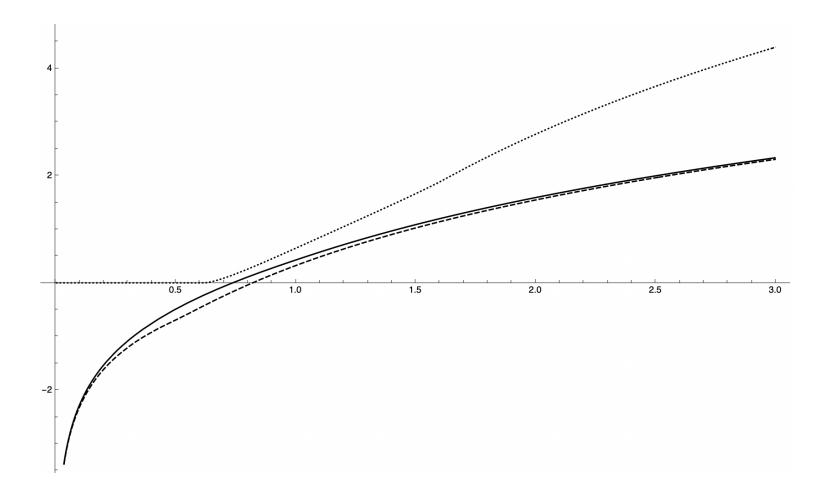
\includegraphics[width=0.8\textwidth]{assets/fig/_page_127_Figure_2.jpeg}
  \caption{针对二价函数 \(\varphi_r(z) = (rz) - (rz)^2\), 重排积分（实线）与 Bost--Charles 积分（虚线）的函数图像. 在它们上方（点线）为 \(2 \int_{\mathbf{T}} \log^+ |\varphi_r| \, \mu_{\text{Haar}}\) 的函数图像.}\label{fig:8.1.15}
\end{figure}

\begin{example}\label{ex:8.1.16}
考虑具有变化半径 r 的函数 \(\varphi_r(z) := rz - (rz)^2\). 
对于 \(r \ge 1\), Bost--Charles 积分等价于:
\[ \iint_{\mathbf{T}^2} \log |\varphi_r(z) - \varphi_r(w)| \, \mu_{\text{Haar}}(z) \mu_{\text{Haar}}(w) = 2 \log r + \int_{\mathbf{T}} \log^+ \left| \frac{r}{1 - rz} \right| \mu_{\text{Haar}}(z) \]
\[ = 2 \log r + \frac{1}{\pi r} + \frac{1}{72\pi r^2} + \dots \]
相比之下, 对重排积分的计算揭示其作为显式函数为:
\[ \int_{0}^{1} 2t \cdot (\log |\varphi_{r}(e^{2\pi it})|)^{*} dt = 2\log r + \frac{1}{2\pi^{2}} \left(8\operatorname{Li}_{3}(1/r) - \operatorname{Li}_{3}(1/r^{2})\right) \]
\[ = 2\log r + \frac{4}{\pi^{2}r} + \frac{4}{27\pi^{2}r^{2}} + \dots \]
这一比较对于 r 的大多数值而言都是非常紧密的, 如\autoref{fig:8.1.15} 所示. 
相比之下, 通过下式给出的 Nevanlinna 特征上界:
\[ 2\int_{\mathbf{T}} \log^+ |\varphi_r| \, \mu_{\text{Haar}} = 2\int_{|z|=r} \log^+ |z - z^2| \, \mu_{\text{Haar}}(z) \]
\[ = 4\log r \quad \text{当 } r \ge \frac{\sqrt{5} + 1}{2} \text{ 时} \]
是非常粗糙的. \end{example}

\begin{remark}\label{rem:8.1.17}
两种增长特征积分在“大”半径 \(|z| = r\) 处的渐近等价性（如在示例 8.1.16 和\autoref{fig:8.1.15} 中所观察到的）似乎是一个相当普遍的特征, 
它反映了膨胀圆周 \(|z| = r\) 的均匀测度 \(\mu_{\text{Haar}}\) 在 \(\varphi_*\) 下推前测度的近乎旋转不变性, 
这考虑到通过切片不等式 \eqref{eq:8.1.12} 对命题 8.1.13 的证明. 
一个“在实际中”的例子见于我们在第 14.5 节中对定理 C 的证明. 
在在这种情况下, Bost--Charles 积分 \eqref{eq:A.6.1} 与重排积分 \eqref{eq:A.6.3} 的比较如下:
\[ 9.963 \sim \iint_{\mathbf{T}^2} \log |\varphi(z) - \varphi(w)| \, \mu_{\text{Haar}}(z, w) \leq \int_0^1 2t \cdot (\log |\varphi(e^{2\pi i t})|)^* \, dt \, \sim 9.972, \]
这是一个仅在千分之几数量级上的改进.
（相比之下, 来自 \eqref{eq:B.0.2} 的 Nevanlinna 特征量 \(2T(\varphi) = 2 \int_{\mathbf{T}} \log^+ |\varphi| \mu_{\mathrm{Haar}}\) 在当前情况下大到 \(\sim 14.08\).）

这一类的另一个例子可以通过比较源于定理 6.0.2 以及定理 7.6.4 的、在定理 A 的两个证明中出现的上界来观察到. 
通过定理 6.0.2 的证明（带有两个划分点, 参见第 13 节）给出了关于重排积分形式的边界 \(m < 13.731\). 
在另一方面, 定理 7.6.4 给出了关于算术相交数形式的边界, 
这些相交数可表示为作为 Bost--Charles 积分轻微推广的积分（参见引理 7.4.5）. 
伴随着对划分点类似的选取, 这导致了边界 \(m < 13.679\) （参见示例 7.6.8, 特别是公式 \eqref{eq:7.6.9}）, 
这是一个小于百分之零点五的改进. 
由于凸性论证引起的积分和边界的轻微修改形式, 这一比较字面上并不是命题 8.1.13 的例子. 
然而, 它准确地反映了我们在没有凸性下数值上观察到的、在重排积分和 Bost--Charles 积分之间的改进程度. \end{remark}

\subsection{定理 8.0.1 的证明}\label{sec:8.2}

我们首先证明 \eqref{eq:8.0.4}, 它将 \eqref{eq:8.0.3} 作为一个特殊情况包含在内. 
我们将在最后讨论如何修改证明以获得 \eqref{eq:8.0.5}.

对于下文, 我们固定一个 \(\epsilon > 0\) 以及变量个数 d. 
仅仅在证明的最后, 我们将首先令 \(d \to \infty\), 随后令 \(\epsilon \to 0\). 
为了与第 6 节和 \eqref{eq:6.0.10} 进行比较, 
我们指出定理 8.0.1 中的边界在使用高维等分布特征的前提下, 在分母中仅具有 \(\tau^{\flat\flat}(\mathbf{b})\), 
而其他项与第 7 节中推导出的单变量边界是相同的. 
因此, 为了证明定理 8.0.1, 我们只需要纳入在 \(\prod_{j=1}^d f_{i_j}(x_j)\) 中均衡指标 \(\mathbf{i} = (i_1, \dots, i_d)\) 的特征, 
而我们不需要像第 6.2 节中那样在 \(\mathbf{x}^{\mathbf{k}}\) 中使用等分布的次数 k. 
这启发了我们要作为我们的评估模基础的欧几里得格的以下选择.

\subsubsection{欧几里得格}\label{sec:8.2.1}

考虑自由 \(\mathbf{Z}\)-模:
\begin{equation}\label{eq:8.2.2}
E_D := \bigoplus_{\mathbf{i} \in V_m^d(\epsilon)} f_{\mathbf{i}}(\mathbf{x}) \mathbf{Z}[1/x_1, \dots, 1/x_d]_{\leq D},
\end{equation}
其中我们召回, 子集 \(V_m^d(\epsilon) \subset \{1, \dots, m\}^d\) （取决于固定的微小正整常数 \(\epsilon\)）定义为
\[
\begin{aligned}
V_m^d(\epsilon) = \Big\{ \mathbf{i} \in \{1, \dots, m\}^d &: \forall i_0 \in \{1, \dots, m\}, \\
& d/m - \epsilon d < \#\{1 \le j \le d \mid i_j = i_0\} < d/m + \epsilon d \Big\};
\end{aligned}
\]
并且按惯例, \(f_{\mathbf{i}}(\mathbf{x}) := \prod_{j=1}^d f_{i_j}(x_j)\). 
在此, \(\mathbf{Z}[1/x_1, \dots, 1/x_d]_{\leq D}\) 表示由 \(1/x_1, \dots, 1/x_d\) 组成的整多项式组成的自由 \(\mathbf{Z}\)-模, 
其中所有的偏次数——对于每个 \(1/x_j\)——都至多为 D.

根据构造, 有 \(\operatorname{rank} E_D = (D+1)^d \cdot \#V_m^d(\epsilon)\). 
根据定理 4.2.1（实际上, 大数弱定律在此处已足够）, 我们有:
\[ \lim_{d\to\infty} \frac{\#V_m^d(\epsilon)}{m^d} = 1, \quad \text{因此} \quad \lim_{d\to\infty} \lim_{D\to\infty} \frac{\operatorname{rank} E_D}{m^d D^d} = 1. \]

为了赋予 \(E_D\) 适当的范数, 我们考虑光滑射影算术方案 \(\mathcal{X} := (\mathbf{P}_{\mathbf{Z}}^1)^d\) 
以及在 \(\mathcal{X}\) 上的自然极宽裕线丛 \(\mathcal{L} := \otimes_{j=1}^d \operatorname{pr}_j^* \mathcal{O}(1)\), 
其中 \(\operatorname{pr}_j : \mathcal{X} \to \mathbf{P}_{\mathbf{Z}}^1\) 表示投影到第 j 个分量上的态射. 
那么我们可以将 \(\Gamma(\mathcal{X}, \mathcal{L}^{\otimes D})\) 识别为 \(\mathbf{Z}[1/x_1, \ldots, 1/x_d]_{\leq D}\), 
其中 \(x_j := Y_j/Z_j\) 是第 j 个 \(\mathbf{P}_{\mathbf{Z}}^1 = \operatorname{Proj} \mathbf{Z}[Y_j, Z_j]\) 的仿射坐标.

召回我们被给予了一个全纯映射 \(\varphi: (\overline{\mathbf{D}}, 0) \to (\mathbf{P}^1(\mathbf{C}), 0)\), 
其中 ``0'' 可以意味着对于每个在 \(\mathcal{X}_{\mathbf{C}}\) 中的 \(\mathbf{P}^1_{\mathbf{C}}\) 副本均有 \(x_j = 0\). 
来自第 7.3.1 节的 Bost--Charles 度量因此通过在每个因子 \(\operatorname{pr}^*_j \, \mathcal{O}(1)\) 上使用 \(\varphi\) 来定义. 
这在 \(\mathcal{L}\) 上诱导了一个 Hermitian 线丛结构 \(\overline{\mathcal{L}} = (\mathcal{L}, \|\cdot\|_{\overline{\mathcal{L}}})\), 
并且反过来, 如同在第 7.3.3 节中一样, 在我们固定了 \((\mathbf{P}^1)^d(\mathbf{C})\) 上的光滑概率测度 \(\nu\) 之后, 
在 \(\mathbf{Z}\)-模 \(\Gamma(\mathcal{X}, \mathcal{L}^{\otimes D})\) 上定义了一个欧几里得格 \(\Gamma_{L^2}\left(\mathcal{X}, \nu; \overline{\mathcal{L}}^{\otimes D}\right)\). 
\(\nu\) 的选择对于证明是无足轻重的, 
因为我们只需在固定的 \(\nu\) 下令 \(D \to \infty\), 
并且我们只需要研究由对于 \(\widehat{\deg} \Gamma_{L^2}\left(\mathcal{X}, \nu; \overline{\mathcal{L}}^{\otimes D}\right)\) 
的算术 Hilbert--Samuel 公式给出的渐近领先阶数项. 
具体而言, 我们选取 \(\nu\) 为光滑测度:
\[
\begin{aligned}
\nu &:= \bigwedge_{j=1}^{d} \operatorname{pr}_{j}^{*} \omega_{\mathrm{FS}} \\
&= \left(\frac{\sqrt{-1}}{2\pi}\right)^{d} \frac{dz_{1} \wedge \cdots \wedge dz_{d} \wedge d\bar{z}_{1} \wedge \cdots \wedge d\bar{z}_{d}}{\prod_{j=1}^{d} (1+|z_{j}|^{2})^{2}},
\end{aligned}
\]
伴随着 \(\omega_{\text{FS}} = \frac{\sqrt{-1}}{2\pi} \frac{dz \wedge d\bar{z}}{(1+|z|^2)^2}\) 为在 \(\mathbf{P}^1(\mathbf{C})\) 上的 Fubini--Study 形式. 
那么, 如第 7.3.3 节所示, 在 \(\Gamma\left(\mathcal{X},\overline{\mathcal{L}}^{\otimes D}\right)\) 上的欧几里得范数 \(\|\cdot\|\) 由下式定义:
\begin{equation}\label{eq:8.2.3}
||s|| := \sqrt{\int_{\mathcal{X}(\mathbf{C})} ||s||_{\mathcal{L}}^2 \nu}.
\end{equation}

正如在第 7.3.3 节中一样, 我们取以下由 \eqref{eq:8.2.3} 在 \(\Gamma\left(\mathcal{X}, \overline{\mathcal{L}}^{\otimes D}\right)\) 上的诱导范数所给出的欧几里得格的正交直和 \eqref{eq:8.2.2}:
\[
\begin{aligned}
&\mathbf{Z}[1/x_1,\ldots,1/x_d]_{\leq D} \\
&\quad \cong \Gamma(\mathcal{X},\mathcal{L}^{\otimes D}) \subset \Gamma(\mathcal{X},\mathcal{L}^{\otimes D})_{\mathbf{R}}.
\end{aligned}
\]
我们将这一欧几里得格记为 \(\overline{E}_D = (E_D, \|\cdot\|)\).

\subsubsection{算术度}\label{sec:8.2.4}

直接像到 Spec \(\mathbf{Z}\) 的算术度的渐近计算是算术 Hilbert--Samuel 公式的研究主题:

\begin{lemma}\label{lem:8.2.5}
当 \(D \to \infty\) 时, 我们有关于算术度如下的渐近性:
\begin{equation}\label{eq:8.2.6}
\widehat{\operatorname{deg}} \, \Gamma_{L^{2}} \left( \mathcal{X}, \nu; \overline{\mathcal{L}}^{\otimes D} \right) = \frac{d}{2} \left( \overline{\mathcal{O}(1)} \cdot \overline{\mathcal{O}(1)} \right) D^{d+1} + o(D^{d+1}),
\end{equation}
\[ \widehat{\operatorname{deg}} \, \overline{E}_{D} = \frac{d \# V_{m}^{d}(\epsilon)}{2} \left( \overline{\mathcal{O}(1)} \cdot \overline{\mathcal{O}(1)} \right) D^{d+1} + o(D^{d+1}). \]
\end{lemma}

\begin{proof}
作为欧几里得格, \(\Gamma(\mathcal{X}, \overline{\mathcal{L}}^{\otimes D}) \cong \bigotimes_{j=1}^{d} \Gamma\left(\mathbf{P}_{\mathbf{Z}}^{1}, \overline{\mathcal{O}(1)}^{\otimes D}\right)\), 
其中每一因子 \(\Gamma\left(\mathbf{P}_{\mathbf{Z}}^{1}, \overline{\mathcal{O}(1)}^{\otimes D}\right)\) 上的范数都是使用 Hermitian 线丛 \(\overline{\mathcal{O}(1)}\) 
以及在 \(\mathbf{P}^1(\mathbf{C})\) 上的 Fubini--Study 形式 \(\omega_{\text{FS}}\) 的 \(L^2\)-范数. 
因此, 根据引理 7.2.7, 我们有
\[ \widehat{\operatorname{deg}}\,\Gamma\left(\mathcal{X},\overline{\mathcal{L}}^{\otimes D}\right) = d(D+1)^{d-1}\widehat{\operatorname{deg}}\,\Gamma\left(\mathbf{P}_{\mathbf{Z}}^{1},\overline{\mathcal{O}(1)}^{\otimes D}\right). \]
现在, 第一个断言源于算术 Hilbert--Samuel 公式 \eqref{eq:7.3.4}. 
第二个断言根据 \eqref{eq:7.2.4} 源于第一个断言.
\end{proof}

\begin{remark}\label{rem:8.2.7}
这一计算的证明也是 Krull 维度为 d+1 的一般算术 Hilbert--Samuel 公式的推论. 
在 \cite[定理 1.4]{Zha95} 中, 算术 Hilbert--Samuel 公式对于任意维度的算术簇以及配备有逐点非负 Chern 形式的光滑度量的宽裕 Hermitian 线丛得到了证明. 
利用 \cite[第 5 节]{Bos99} 和 \cite[第 3--4 节]{BC22} 中的想法, 
相同的公式对于在任意维度的算术簇上、配备有逐点非负 Chern 形式的 \(\mathcal{C}^{\mathrm{b}\Delta}\) Hermitian 度量的宽裕线丛仍然是成立的. 
因此我们也可以直接从关于 \((\mathcal{X}, \overline{\mathcal{L}})\) 的算术 Hilbert--Samuel 公式推导引理 8.2.5:
\[ \widehat{\operatorname{deg}}\,\Gamma_{L^2}\left(\mathcal{X},\nu;\overline{\mathcal{L}}^{\otimes D}\right) = \frac{\overline{\mathcal{L}}^{d+1}}{(d+1)!}D^{d+1} + o(D^{d+1}). \]
在此, \(\overline{\mathcal{L}}^{d+1}\) 表示算术自相交数 \(\widehat{c}_1(\overline{\mathcal{L}})^{d+1}.[\mathcal{X}]\). 
在我们的设定中, 我们写出 \(\overline{\mathcal{L}} = \otimes_{j=1}^d \operatorname{pr}_j^* \overline{\mathcal{O}(1)}\), 
并通过多线性展开自相交数. 唯一非零项来自于对除了一个 \(\operatorname{pr}_{i}^{*}\mathcal{O}(1)\) 因子之外的所有因子穿过一次, 
以及对剩下的这一个 \(\operatorname{pr}_{i}^{*}\mathcal{O}(1)\) 因子穿过两次. 
根据投影公式, 这为我们提供了
\[ \overline{\mathcal{L}}^{d+1} = d \binom{d+1}{2} (d-1)! \left( \overline{\mathcal{O}(1)} \cdot \overline{\mathcal{O}(1)} \right), \]
并且我们以此透视同样恢复了引理 8.2.5. \end{remark}

\subsubsection{评估过滤}\label{sec:8.2.8}

记 \(X := \mathcal{X}_{\mathbf{Q}}\), 我们可以将 \(\operatorname{Spf} \mathbf{Q}[\![x]\!] = \widehat{X}_0\) 识别为 X 在其闭子模式 0 处的形式完备化, 
这特别地对于 \(i = 1, \dots, m\) 给出了元素
\[ f_{\mathbf{i}} = f_{\mathbf{i}}(\mathbf{x}) \in \Gamma(\widehat{X}_0, \mathcal{O}_{\widehat{X}_0}). \]
\(\mathcal{L}^{\otimes D}|_{\widehat{X}_0}\) 的全局截面空间 \(\Gamma\left(\widehat{X}_0, \mathcal{L}^{\otimes D}\right)\) 随后被自然地识别为:
\[
\begin{aligned}
\Gamma\left(\widehat{X}_0, \mathcal{L}^{\otimes D}\right) &= \mathbf{x}^{-D}\mathbf{Q}[\![\mathbf{x}]\!] \\
&=: F_{\mathbf{Q}},
\end{aligned}
\]
其中 \(\mathbf{x}^{-D}\mathbf{Q}[\![\mathbf{x}]\!]\) 表示由满足对于所有 \(1 \leq j \leq d\) 均有 \(k_j \geq -D\) 
的 \(\mathbf{x}^{\mathbf{k}}\) 组成的 \(\mathbf{Q}\)-向量空间. 
因此 \(f_{\mathbf{i}} \Gamma(\mathcal{X}, \mathcal{L}^{\otimes D}) \subset \Gamma(\widehat{X}_0, \mathcal{L}^{\otimes D})\), 
并且我们有单射评估映射:
\[ \psi_D: E_D \hookrightarrow F_{\mathbf{Q}}, \quad (Q_{\mathbf{i}})_{\mathbf{i} \in V_m^d(\epsilon)} \mapsto \sum_{\mathbf{i} \in V_m^d(\epsilon)} f_{\mathbf{i}} Q_{\mathbf{i}}, \]
此处的 \(Q_{\mathbf{i}} \in \Gamma(\mathcal{X}, \mathcal{L}^{\otimes D})\) 且 \((Q_{\mathbf{i}})_{\mathbf{i} \in V_m^d(\epsilon)} \in E_D\). 
与第 3.1.3 节类似, 我们首先使用总消逝阶数、随后在每个射流空间（jet space）内使用字典序来过滤 \(F_{\mathbf{Q}}\):
\[ F_{\mathbf{Q}} = F_{\mathbf{Q}}^{(\mathbf{0})} \supseteq \cdots \supseteq F_{\mathbf{Q}}^{(\mathbf{n})} \supseteq \cdots, \]
其中 \(\mathbf{n} \in \mathbf{N}^d\), 并且 \(F_{\mathbf{Q}}^{(\mathbf{n})} := \operatorname{Span}_{\mathbf{Q}}\{\mathbf{x}^{\mathbf{m}} : \mathbf{n} \prec \mathbf{m} + D \text{ 或 } \mathbf{n} = \mathbf{m} + D\}\). 
在此处, \(\mathbf{N}^d\) 上的总序 \(\prec\) 定义在第 3.1.3 节中, 并且对于 \(\mathbf{m} = (m_j)_{j=1}^d\), 
我们定义 \(\mathbf{m} + D := (m_j + D)_{j=1}^d\). 
用于定义字典序的变量 \(x_1, \ldots, x_d\) 的顺序对于证明是无足轻重的. 
在这一 \(\prec\)-过滤记号下, 由于 \(\prod_{j=1}^d x_j^{-D} \in \Gamma(\mathcal{X}, \mathcal{L}^{\otimes D})\) 
是 \(\mathcal{L}_0^{\otimes D}\) 的一个生成元（此处我们用 \(\mathcal{L}_0\) 表示 \(\mathcal{L}\) 到 \(\mathbf{Z}\)-点 \(\mathbf{x} = \mathbf{0}\) 的限制）, 
我们观察到：一个形式截面 \(g(\mathbf{x}) \in F_{\mathbf{Q}} = \Gamma(\widehat{X}_0, \mathcal{L}^{\otimes D})\) 
在 \(\mathbf{x} = \mathbf{0}\) 处的消逝阶数 \(\operatorname{ord}_0(g(\mathbf{x}))\) （作为 \(\mathcal{L}^{\otimes D}|_{\widehat{X}_0}\) 的正则截面, 
而不是作为 \(\mathbf{x}^{-D}\mathbf{Q}[\![\mathbf{x}]\!]\) 中的 Laurent 级数） 
至少为 n, 当且仅当 \(g(\mathbf{x}) \in F_{\mathbf{Q}}^{(0,\ldots,0,n)}\). 
我们还观察到 \(g(\mathbf{x}) \in F_{\mathbf{Q}}^{(\mathbf{n})}\) 当且仅当要么 \(\operatorname{ord}_0(g(\mathbf{x})) > |\mathbf{n}|\), 
要么 \(\operatorname{ord}_0(g(\mathbf{x})) = |\mathbf{n}|\) 并且在 g 的齐次度为 \(|\mathbf{n}|\) 的部分中最低字典序项具有指数向量 \(\mathbf{m}\), 
使得 \(\mathbf{n} \prec \mathbf{m}\). 
（如果在此处人们更倾向于将 g 视为 \(\mathbf{x}^{-D}\mathbf{Q}[\![\mathbf{x}]\!]\) 中的 Laurent 级数, 
而不是作为 \(\mathcal{L}^{\otimes D}|_{\widehat{X}_0}\) 的形式截面, 
那么在这些陈述中, 人们将不得不把所有的指数向量 \(\mathbf{n}\) 平移到 \(\mathbf{n} - D\).）

与第 3.1.3 节类似, 我们用 \(\mathbf{n}^+\) 表示 \(\mathbf{n}\) 在总序 \(\prec\) 下的后继. 
Graded 分量 \(F_{\mathbf{Q}}^{(\mathbf{n})}/F_{\mathbf{Q}}^{(\mathbf{n}^+)}\) 是一个一维 \(\mathbf{Q}\)-向量空间, 
由商映射下 \(\mathbf{x}^{\mathbf{n}-D}\) 的像所生成. 
在 \(F_{\mathbf{Q}}^{(\mathbf{n})}/F_{\mathbf{Q}}^{(\mathbf{n}^+)}\) 上的欧几里得格结构由商映射下 \(\mathbf{x}^{\mathbf{n}-D}\) 
的像所生成的自由秩 1 \(\mathbf{Z}\)-模以及满足 \(\|\mathbf{x}^{\mathbf{n}-D}\| = 1\) 的欧几里得范数所给出. 
除了在 x 的幂次中有一个 \(-D\) 的移动之外, 这与第 7.3 节中是相同的.

正如在第 7.3 节中一样, 我们拥有自然的单射评估映射 \(\psi_D: E_D \to F_{\mathbf{Q}}\), 
这在 graded 分量上诱导了单射:
\[ \psi_D^{(\mathbf{n})}: E_D^{(\mathbf{n})}/E_D^{(\mathbf{n}^+)} \hookrightarrow F_{\mathbf{Q}}^{(\mathbf{n})}/F_{\mathbf{Q}}^{(\mathbf{n}^+)}. \]
因此对于所有 \(\mathbf{n} \in \mathbf{N}^d\), 
均有 \(\operatorname{rank} E_D^{(\mathbf{n})}/E_D^{(\mathbf{n}^+)} \in \{0,1\}\). 
令
\[ \mathcal{V}_D^d := \{ \mathbf{n} \in \mathbf{N}^d \mid \operatorname{rank} E_D^{(\mathbf{n})} / E_D^{(\mathbf{n}^+)} = 1 \} \]
为消逝过滤跳跃集合. 我们有 \(\#\mathcal{V}_D^d = \operatorname{rank} E_D\).

在接下来的第 8.2.11 节和第 8.2.29 节中, 我们提供关于在所有 \(v \in M_{\mathbf{Q}}\) 处的局部评估高度 \(h_v(\psi_D^{(\mathbf{n})})\) 的上界估计. 
根据局部评估高度的定义, 我们需要考虑任意的 \((Q_{\mathbf{i}})_{\mathbf{i} \in V_m^d(\epsilon)} \in E_D^{(\mathbf{n})} \setminus E_D^{(\mathbf{n}^+)}\), 
并随后提供 \(\log |c_{\mathbf{n}}|_v - \log ||(Q_{\mathbf{i}})_{\mathbf{i} \in V_m^d(\epsilon)}||_{E_D,v}\) 的上界, 
其中 \(c_{\mathbf{n}}\) 表示在 \(s := \sum_{\mathbf{i} \in V_m^d(\epsilon)} f_{\mathbf{i}}Q_{\mathbf{i}}\) 中 \(\mathbf{x}^{\mathbf{n}-D}\) 的系数. 
在此处, \(|c_{\mathbf{n}}|_v\) 表示在 \(\mathbf{Q}\) 上的常用 v-进范数.

\begin{definition}\label{def:8.2.9}
对于域 k 上的形式幂级数 \(F(t_1, \ldots, t_d) \in k[\![t_1, \ldots, t_d]\!] = \sum_{\mathbf{n}} a_{\mathbf{n}} \mathbf{t}^{\mathbf{n}}\), 
F 的 n-阶射流（jet）是由所有次数为 n 的项之和给出的、次数为 n 的齐次多项式 \(J_n(F) \in k[t_1, \ldots, t_d]_{(n)}\):
\[ J_n(F)(t_1,\ldots,t_d) := \sum_{| \mathbf{n} | = n} a_{\mathbf{n}} \mathbf{t}^{\mathbf{n}} \in k[\mathbf{t}]_{(n)}. \]
\end{definition}

\begin{remark}\label{rem:8.2.10}
在关于高维形式解析算术簇代数化的早期工作 \cite{Bos01}\cite{Bos04} 中, 
仅使用在点 \(\mathbf{0}\) 处的总消逝阶数来过滤辅助评估模就已经足够了. 
我们在此使用具有一维商的更精细过滤, 该做法具有两个优势:
\begin{itemize}
  \item[(1)] 对于在阿基米德地方 v 处 \(h_v\) 的估计, 
  利用 \(\overline{\mathbf{D}}^d \to \mathcal{X}(\mathbf{C})\) 的乘积结构, 
  我们拥有与 \cite[引理 2.4.1]{CDT21} 类似的一个容易的“逐个变量”次调和估计. 
  这避免了 \cite[第 4.3.2 节]{Bos01} 中的吹起方法, 
  后者给出了领先阶数射流多项式 \(J_n(F) \in \mathbf{Q}[\mathbf{x}]_{(n)}\) 的 Mahler 测度的上界, 
  而需要被估计的量是该领先阶数射流中单个系数 \(c_{\mathbf{n}}\) 的大小. 
  在维度 \(d = \dim \mathcal{X}_{\mathbf{Q}}\) 中, 这些量的差异是非常敏感的, 
  维度 d 在 \cite{Bos01} 中是固定的, 
  而在我们的方法中, 我们希望最后令 \(d \to \infty\).
  \item[(2)] 在非阿基米德地方 v 处对 \(h_v\) 估计的优势是至关重要的. 
  在满足 \(|\mathbf{n}| = n\) 的所有 \(\mathbf{n}\) 中, 
  由于我们对 \(E_D\) 的特定构造, 我们在 \(\{n_j\}_{j=1}^d\) 渐近等分布分量的条件下将拥有对 \(h_v\left(\psi_D^{(\mathbf{n})}\right)\) 的好得多的估计. 
  我们包含字典序的完全过滤允许我们利用这一改进. \end{itemize}
\end{remark}

\subsubsection{阿基米德估计}\label{sec:8.2.11}

召回通过与引理 7.4.1 证明开端的相同简化论证, 
我们对于所有 \(1 \le i \le m\), 都可以假设 \(f_i(\varphi(z))\) 
在 \(|z| \le 1\) 的一个开邻域上是亚纯的.

为了方便记号, 我们用 \(|\cdot|\) 表示常用绝对值 \(|\cdot|_{\infty}\). 
证明的更宽框架与 \cite[第 4.3.3 节]{Bos01} 类似, 
并带有着我们在注记 8.2.10(1) 中描述的修改. 
给定 \(s \in \psi_D^{(\mathbf{n})}(E_D^{\mathbf{n}} \setminus E_D^{\mathbf{n}^+})\), 
我们将遵循 \cite[第 2.4 节]{CDT21} 中关于研究在点 \(\mathbf{z} = \mathbf{0} \in \overline{\mathbf{D}}^d\) 
处的 \(n\)-阶（领先）射流 \(J_n(\varphi^*s)(\mathbf{z}) \in \mathbf{C}[\mathbf{z}]_{(n)}\). 
在此处以及在下文中, 我们使用记号 \(n := |\mathbf{n}|\), 
并且伴随着对记号的轻微滥用, 我们继续用 \(\varphi : \overline{\mathbf{D}}^d \to \mathcal{X}(\mathbf{C})\) 
表示在每个因子上对角定义的解析态射 \(\mathbf{x} \mapsto (\varphi(z_1), \dots, \varphi(z_d))\) （此处 \(\varphi : \overline{\mathbf{D}} \to \mathbf{C}\)）. 
通过该记号的推广, 并且以统一第 6 节和第 7.4 节的方式, 
我们对于每个 \(\mathbf{r} \in (0, 1]^d\) 考虑解析态射:
\[ \varphi_{\mathbf{r}}: \overline{\mathbf{D}}^d \to \mathbf{C}^d \hookrightarrow \mathcal{X}(\mathbf{C}), \qquad \mathbf{z} \mapsto (\varphi(r_1 z_1), \dots, \varphi(r_d z_d)). \]
我们将使用 Poisson--Jensen 公式通过射流函数来约束 \(\log |c_{\mathbf{n}}|\), 
随后借助 Poincaré--Lelong 公式将产生的边界与 \(\overline{\mathcal{L}}\) 的 Chern 形式联系起来. 
我们遵循第 7.4 节中的记号, 并且我们从 \eqref{eq:7.1.7} 借用斜率 \(\alpha_k\) 的记号. 
此外, 对于每个 \(\mathbf{n} \in \mathbf{N}^d\), 我们定义 \(r(\mathbf{n}) := (r(n_1), \ldots, r(n_d))\), 
其中
\begin{equation}\label{eq:8.2.12}
r(t) := \begin{cases} r_k, & t/D \in [\alpha_k, \alpha_{k+1}), \\ 1, & t/D > m. \end{cases}
\end{equation}

通篇本节, \(\mathbf{z} = (z_1, \dots, z_d)\) 表示 \(\overline{\mathbf{D}}^d\) 上的坐标. 
我们使用通过 \(\mathbf{x}^{-D} \mapsto \mathbf{1}\) 给出的、\(\mathcal{L}^{\otimes D}\) 在 \(\mathbf{A}^d_{\mathbf{C}}\) 
上的平凡化 \(\mathcal{L}^{\otimes D}|_{\mathbf{C}^d} \stackrel{\simeq}{\to} \mathcal{O}_{\mathbf{C}^d}\). 
在此识别下, \(s/\mathbf{x}^{-D} = s \cdot \mathbf{x}^D =: G(\mathbf{x})\) 
自然在 \(\Gamma(\widehat{X}_0, \mathcal{O}_{\widehat{X}_0})\) 中且消逝阶数为 n. 
由于我们解析的 \(\varphi_{r(\mathbf{n})}\)-拉回是由 \(x_j = \varphi_{r(n_j)}(z_j) = (\varphi'(0) \cdot r(n_j))z_j + O(z_j^2)\) 定义的, 
我们根据构造有 \(\varphi^*_{r(\mathbf{n})}G\) 具有 \(\mathbf{z} = \mathbf{0}\) 消逝阶数 n, 
并且在 \(J_n\left(\varphi_{r(\mathbf{n})}^*G\right)\) 
中（以及在 \(\varphi_{r(\mathbf{n})}^*G\) 中的整体 \(\prec\)-极小项） 
以 \(c_{\mathbf{n}}\varphi'(0)^n \prod_{j=1}^d r(n_j) \mathbf{z}^{\mathbf{n}}\) 
为字典序极小项. 
然而, 由于我们在此定理中仅假设了拉回函数的*亚纯性*（而不是全纯性）： \(\varphi^*f_i \in \mathcal{M}(\overline{\mathbf{D}})\), 
解析芽 \(\varphi_{r(\mathbf{n})}^*G \in \mathbf{C}[\![\mathbf{z}]\!]\) 
仅亚纯地（而不是全纯地）延拓通过 \(\overline{\mathbf{D}}\). 
但如果我们选择全纯函数 \(h \in \mathcal{O}(\overline{\mathbf{D}})\), 
满足 \(h(0) = 1\) 且所有的 \(h \cdot \varphi^*f_i \in \mathcal{O}(\overline{\mathbf{D}})\) 都是全纯的, 
那么 \(h(z_1) \cdots h(z_d) \cdot \left(\varphi_{r(\mathbf{n})}^*\right) G(\mathbf{z}) \in \mathcal{O}\left(\overline{\mathbf{D}}^d\right)\) 
在整个 \(\overline{\mathbf{D}}^d\) 上是全纯的, 
并且具有与 \(\varphi_{r(\mathbf{n})}^*G\) 相同的领先阶数射流 \(J_n\left(\varphi_{r(\mathbf{n})}^*G\right)\).

这使我们可以利用 \cite[引理 2.4.1]{CDT21} 来根据齐次多项式 \(J_n\left(\varphi_{r(\mathbf{n})}^*G\right) = J_n\left(h(z_1)\cdots h(z_d)\cdot \varphi_{r(\mathbf{n})}^*G\right)\) 
的 Mahler 测度来上估计所必需的系数 \(|c_{\mathbf{n}}|\), 
在其中显然整体上字典序最低的项是在多重次数 \(\mathbf{n}\) 中的单项式 \(c_{\mathbf{n}}\mathbf{z}^{\mathbf{n}}\):
\begin{equation}\label{eq:8.2.13}
\begin{aligned}
\log |c_{\mathbf{n}}| &\leq -n \log |\varphi'(0)| - \sum_{j=1}^{d} n_{j} \log r(n_{j}) \\
&\quad + \int_{\mathbf{T}^{d}} \log \left| J_{n} \left( h(z_{1}) \cdots h(z_{d}) \cdot \varphi_{r(\mathbf{n})}^{*} G \right) \right| \mu_{\text{Haar}}.
\end{aligned}
\end{equation}

我们可以将此与 Bost 在 \cite[引理 4.13 中的等式 (4.28)]{Bos01} 中的吹起论证联系起来, 该论证显示:
\begin{equation}\label{eq:8.2.14}
\begin{aligned}
&\int_{\mathbf{T}^d} \log \left| J_n \left( h(z_1) \cdots h(z_d) \cdot \varphi_{r(\mathbf{n})}^* G \right) \right| \mu_{\text{Haar}} \\
&\quad \leq \int_{\mathbf{T}^d} \log \left| h(z_1) \cdots h(z_d) \cdot \varphi_{r(\mathbf{n})}^* G \right| \mu_{\text{Haar}} \\
&\quad = \int_{\mathbf{T}^d} \log \left| \varphi_{r(\mathbf{n})}^* G \right| \mu_{\text{Haar}} + O_h(1).
\end{aligned}
\end{equation}
为了回顾 Bost 的论证, 写出 \(h(z_1) \cdots h(z_d) \cdot G(\varphi_{r(\mathbf{n})}^*(\mathbf{z})) =: \sum_{\mathbf{k} \in \mathbf{N}^d} c_{\mathbf{k}}' \mathbf{z}^{\mathbf{k}}\), 并定义:
\begin{equation}\label{eq:8.2.15}
U_t(\mathbf{z}) := \sum_{\mathbf{k} \in \mathbf{N}^d} c_{\mathbf{k}}' t^{|\mathbf{k}| - n} \mathbf{z}^{\mathbf{k}}, \quad \text{对于满足 } |t| \le 1 \text{ 的 } t \in \mathbf{C}.
\end{equation}
那么, 通过 \(\mathbf{z} \mapsto t\mathbf{z}\) 代换有:
\begin{equation}\label{eq:8.2.16}
\begin{aligned}
&\int_{\mathbf{T}^d} \log |U_t(\mathbf{z})| \, \mu_{\text{Haar}}(\mathbf{z}) \\
&= \int_{|t|\mathbf{T}^d} \log \left| h(z_1) \cdots h(z_d) \right. \\
&\quad \cdot \left. \varphi_{r(\mathbf{n})}^* G \right| \, \mu_{\text{Haar}}(\mathbf{z}) - n \log |t|.
\end{aligned}
\end{equation}
特别地, \(\int_{\mathbf{T}^d} \log |U_t(\mathbf{z})| \, \mu_{\text{Haar}}(\mathbf{z})\) 根据 \eqref{eq:8.2.15} 
显然是单复变量 t 的次调和函数, 
其仅通过等式 \eqref{eq:8.2.16} 右手边的等式依赖于该复变量 t （通过 \(|t|\)）. 
因此, 该函数在 t = 1 处的值（等于 \(\int_{\mathbf{T}^d} \log |h(z_1) \dots h(z_d) \cdot \varphi_{r(\mathbf{n})}^* G |\mu_{\text{Haar}}|\), 
但也是 \(\int_{\mathbf{T}^d} \log |U_t(\mathbf{z})| \, \mu_{\text{Haar}}(\mathbf{z})\) 在 \(t \in \mathbf{T}\) 上的积分） 
不小于其在 t = 0 处的值, 
后者正是所需边界 \eqref{eq:8.2.14} 的左手边.

接下来我们遵循 \cite[定理 10.5.3]{Bos20} 的证明想法, 
以及 \cite[第 4.2--4.3 节]{BC22} 中的讨论, 以便从光滑 Green 函数通过 \(\mathcal{C}^{b\Delta}\) 函数. 
通过 \(\overline{\mathcal{L}}\) 的乘积结构和引理 7.4.1 证明中的计算, 我们有:
\begin{equation}\label{eq:8.2.17}
\begin{aligned}
&\int_{\mathbf{T}^{d}} \log \|\varphi_{r(\mathbf{n})}^{*} \mathbf{x}^{-D}\|_{(\varphi_{r(\mathbf{n})}^{*}\overline{\mathcal{L}})} \mu_{\text{Haar}} \\
&= \sum_{j=1}^{d} \int_{\mathbf{T}} \log \|\varphi_{r(n_{j})}^{*}(x_{j}^{-D})\|_{\overline{\mathcal{O}(D)}} \mu_{\text{Haar}} \\
&= \sum_{j=1}^{d} \left( -\int_{\overline{\mathbf{D}}} \log^{+} |z|^{-1} c_{1} \left( \varphi_{r(n_{j})}^{*} \overline{\mathcal{O}(D)} \right) \right. \\
&\quad + \left. \|\varphi_{r(n_{j})}^{*}(x^{-D})\|_{\varphi_{r(n_{j})}^{*} \overline{\mathcal{O}(D)}} \Big|_{z=0} \right).
\end{aligned}
\end{equation}
由于 \(x^{-D}|_{x=0}\) 是自由 \(\mathbf{Z}\)-模 \(\mathcal{O}(D)_0\) 的一个 \(\mathbf{Z}\)-生成元, 我们有
\[ \|\varphi_{r(n_j)}^*(x^{-D})\|_{\overline{\mathcal{O}(D)}}\,\Big|_{z=0} = -\widehat{\operatorname{deg}}\,\overline{\mathcal{O}(D)}_0 = -D\,\widehat{\operatorname{deg}}\,\overline{\mathcal{O}(1)}_0. \]

结合 \eqref{eq:8.2.13}, \eqref{eq:8.2.14} 和 \eqref{eq:8.2.17}, 我们有:
\begin{equation}\label{eq:8.2.18}
\begin{aligned}
&\log |c_{\mathbf{n}}| - \int_{\mathbf{T}^{d}} \log \|\varphi_{r(\mathbf{n})}^{*}s\|_{(\varphi_{r(\mathbf{n})}^{*}\overline{\mathcal{L}})} \mu_{\mathrm{Haar}} \\
&\quad \leq -n \log |\varphi'(0)| - \sum_{j=1}^{d} n_{j} \log r(n_{j}) \\
&\qquad + \int_{\mathbf{T}^{d}} \left( \log |\varphi_{r(\mathbf{n})}^{*}G(\mathbf{z})| - \log \|\varphi_{r(\mathbf{n})}^{*}s\|_{\varphi_{r(\mathbf{n})}^{*}\overline{\mathcal{L}}} \right) \mu_{\mathrm{Haar}} + O_{h}(1) \\
&\quad = -n \log |\varphi'(0)| - \sum_{j=1}^{d} n_{j} \log r(n_{j}) - \int_{\mathbf{T}^{d}} \log \|\varphi_{r(\mathbf{n})}^{*}\mathbf{x}^{-D}\|_{(\varphi_{r(\mathbf{n})}^{*}\overline{\mathcal{L}})} \mu_{\mathrm{Haar}} + O_{h}(1) \\
&\quad = -n \log |\varphi'(0)| - \sum_{j=1}^{d} n_{j} \log r(n_{j}) \\
&\qquad + D \left( \sum_{j=1}^{d} \widehat{\deg}(\overline{\mathcal{O}(1)}_{0}) + \int_{\overline{\mathbf{D}}} \log^{+} |z|^{-1} c_{1}(\varphi_{r(n_{j})}^{*}\overline{\mathcal{O}(1)}) \right) + O_{h}(1)
\end{aligned}
\end{equation}
\[ = -n \log |\varphi'(0)| - \sum_{j=1}^{d} n_{j} \log r(n_{j}) + D \sum_{j=1}^{d} \widehat{T}(r(n_{j}), \varphi) + O_{h}(1), \]
其中 \(\widehat{T}(r(n_j), \varphi)\) 是我们定义在 \ref{def:7.1.2} 中的 Bost--Charles 特征, 
并且最后的等号源于对 \cite[命题 7.2.2]{BC22} 投影公式应用于注记 7.3.2 以及引理 7.4.5 中的态射 \((\iota, \varphi_{r(n_j)})\) 得到的. 
我们更详细地阐明最后一步. 
根据 \cite[第 7.1.1.1 节]{BC22} 中 Hermitian 向量丛拉回的定义以及 \cite[等式 6.2.4]{BC22} 中算术相交数的定义, 
我们有:
\[ (\iota, \varphi_{r(n_j)})^* \overline{\mathcal{O}(1)} \cdot ([0], \log^+|z|^{-1}) = \widehat{\operatorname{deg}} \, \overline{\mathcal{O}(1)}_0 + \int_{\overline{\mathbf{D}}} \log^+|z|^{-1} c_1(\varphi^*(\overline{\mathcal{O}(1)})). \]
通过 \cite[命题 7.2.2]{BC22} 的投影公式结合引理 7.4.5, 
我们导出所必需的等式:
\[ (\iota, \varphi_{r(n_j)})^* \overline{\mathcal{O}(1)} \cdot ([0], \log^+ |z|^{-1}) = \widehat{T}(r(n_j), \varphi), \]
并且 \eqref{eq:8.2.18} 的最后一行随之成立.

我们声称, \eqref{eq:8.2.18} 意味着对于任意的 \((Q_{\mathbf{i}})_{\mathbf{i} \in V_m^d(\epsilon)} \in E_D^{(\mathbf{n})} \setminus E_D^{(\mathbf{n}^+)}\), 
具有一致上界:
\begin{equation}\label{eq:8.2.19}
\log |c_{\mathbf{n}}| - \|(Q_{\mathbf{i}})_{\mathbf{i} \in V_m^d(\epsilon)}\| \le -n \log |\varphi'(0)| - \sum_{j=1}^d n_j \log r(n_j) + D \sum_{j=1}^d \widehat{T}(r(n_j), \varphi) + o(D).
\end{equation}

由于 \(\mu_{\text{Haar}}\) 不是 \(\overline{\mathbf{D}}^d\) 上的连续测度, 我们首先通过 \(\overline{\mathbf{D}}\) 上关于因子 [0] 的一组光滑旋转对称 Green 函数序列 \((g_k)_{k\in\mathbf{N}}\) 
来逼近 \(\log^+|z|^{-1}\). 
具体而言, 遵循 \cite[第 268 页]{Bos20}, 我们选择满足 \(\sup (g_k) \subset \mathbf{D}\) 
的 \(g_k \in C^{\infty}(\overline{\mathbf{D}})\), 
使得 \(g_k(z) = g_k(|z|)\) 且 \(g_k - \log^+|z|^{-1} \to 0\) 在 \(\overline{\mathbf{D}}\) 上是一致收敛的. 
遵循与引理 7.4.1 证明中完全相同的论证（例如, 参见 \cite[第 270--271 页]{Bos20} 以了解单维情况）, 
我们写出 \(\frac{i}{\pi}\partial \overline{\partial} g_k = -\delta_0 + \mu_k\), 
其中 \(\mu_k\) 是 \(\overline{\mathbf{D}}\) 上的光滑概率测度, 
并且然后, 记 \(\mu_k^d\) 为由 \(\mu_k\) 在 \(\overline{\mathbf{D}}^d\) 上诱导的乘积测度:
\[
\begin{aligned}
&\int_{\overline{\mathbf{D}}^d} \log \|\varphi_{r(\mathbf{n})}^* \mathbf{x}^{-D}\|_{\varphi_{(r(\mathbf{n})}^* \overline{\mathcal{L}})} \mu_k^d \\
&= -D \sum_{j=1}^d \left( \int_{\overline{\mathbf{D}}} g_k c_1(\varphi_{r(n_j)}^* \overline{\mathcal{O}(1)}) + \widehat{\operatorname{deg}} \overline{\mathcal{O}(1)}_0 \right)
\end{aligned}
\]
\[ = -D \sum_{j=1}^d (\iota, \varphi_{r(n_j)})^* \overline{\mathcal{O}(1)} \cdot ([0], g_k). \]
此外, 由于 \(g_k\) 以及 \(\mu_k\) 是旋转不变的, Poisson--Jensen 公式给出:
\[
\begin{aligned}
&\log |c_{\mathbf{n}}| + n \log |\varphi'(0)| + \sum_{j=1}^{d} n_{j} \log r(n_{j}) \\
&\leq \int_{\overline{\mathbf{D}}^{d}} \left( \log |J_{n}(\varphi_{r(\mathbf{n})}^{*}G)(\mathbf{z})| - \log |\mathbf{z}|^{\mathbf{n}} \right) \mu_{k}^{d}
\end{aligned}
\]
\[ = \int_{\overline{\mathbf{D}}^{d}} \log |J_{n}(\varphi_{r(\mathbf{n})}^{*}G)| \mu_{k}^{d} - n \int_{\overline{\mathbf{D}}} \log |z| \mu_{k}; \]
并且我们先前的论证给出
\[ \int_{\overline{\mathbf{D}}^d} \log |J_n(\varphi_{r(\mathbf{n})}^*G)| \, \mu_k^d \le \int_{\overline{\mathbf{D}}^d} \log |\varphi_{r(\mathbf{n})}^*G| \, \mu_k^d. \]
由于 \(\mu_k\) 在 \(\overline{\mathbf{D}}^d\) 上是光滑的且 \(\overline{\mathbf{D}}^d\) 是紧的, 
存在一个仅取决于 \(d, g_k, \varphi, \mathbf{r}\) （但独立于 n, D, 以及 s）的常数 \(C_k > 0\), 
使得 \(C_k \varphi_{r(\mathbf{n})}^* \nu = C_k \bigwedge_{j=1}^d \operatorname{pr}_j^* \varphi_{r(n_j)}^* \omega_{\mathrm{FS}} \ge \mu_k^d\) 
作为在 \(\overline{\mathbf{D}}^d\) 上的光滑 \((d, d)\)-形式的逐点不等式成立.

因此, 我们有:
\[ \begin{split} 
&\log \|(Q_{\mathbf{i}})_{\mathbf{i} \in V_m^d(\epsilon)}\| \\ 
&\geq \max_{\mathbf{i} \in V_m^d(\epsilon)} \log \|Q_{\mathbf{i}}\| = \frac{1}{2} \max_{\mathbf{i} \in V_m^d(\epsilon)} \log \int_{\mathcal{X}(\mathbf{C})} \|Q_{\mathbf{i}}\|_{\mathcal{L}}^2 \nu \\ 
&\geq -\frac{1}{2} \log C_k + \frac{1}{2} \max_{\mathbf{i} \in V_m^d(\epsilon)} \log \int_{\overline{\mathbf{D}}^d} \|\varphi_{r(\mathbf{n})}^* Q_{\mathbf{i}}\|_{(\varphi_{r(\mathbf{n})}^* \overline{\mathcal{L}})}^2 \mu_k^d \\ 
&\geq -\frac{1}{2} \log C_k - \log \left\{ m^d (D+1)^d \max_{\substack{1 \leq i \leq m, \\ z \in \overline{\mathbf{D}}}} |f_i(z)|^d \right\} \\
&\quad + \frac{1}{2} \log \int_{\mathbf{D}^d} \|\varphi_{r(\mathbf{n})}^* s\|_{(\varphi_{r(\mathbf{n})}^* \overline{\mathcal{L}})}^2 \mu_k^d \\ 
&> -C_k' - d \log D + \frac{1}{2} \log \int_{\mathbf{D}^d} \|\varphi_{r(\mathbf{n})}^* s\|_{(\varphi_{r(\mathbf{n})}^* \overline{\mathcal{L}})}^2 \mu_k^d \\ 
&\geq -C_k' - d \log D + \int_{\mathbf{D}^d} \log \|\varphi_{r(\mathbf{n})}^* s\|_{(\varphi_{r(\mathbf{n})}^* \overline{\mathcal{L}})}^2 \mu_k^d, 
\end{split} \]
其中 \(C_k' > 0\) 是仅取决于 \(d, m, \{f_i\}, g_k, \varphi, \mathbf{r}\) （但独立于 n, D 和 s）的常数, 
并且最后的项根据平方均值--几何均值不等式（因为 \(\mu_k^d\) 是 \(\overline{\mathbf{D}}^d\) 上的概率测度, 
参见例如 \cite[(1.4.10)]{BGS94}）是成立的.

我们获得:
\begin{equation}\label{eq:8.2.20}
\begin{aligned}
&\log |c_{\mathbf{n}}| - \log \|(Q_{\mathbf{i}})_{\mathbf{i} \in V_m^d(\epsilon)}\| \\
&\le -n \log |\varphi'(0)| - \sum_{j=1}^d n_j \log r(n_j) - n \int_{\overline{\mathbf{D}}} \log |z| \, \mu_k \\
&\quad + D \sum_{j=1}^d (\iota, \varphi_{r(n_j)})^* \overline{\mathcal{O}(1)} \cdot ([0], g_k) + o(D),
\end{aligned}
\end{equation}
这对于任意固定的独立于 k 以及 D 的 \(\gamma \geq 0\) 并且对于所有足够大的 \(k \gg 1\) 均给出了:
\begin{equation}\label{eq:8.2.21}
\begin{aligned}
&\limsup_{\substack{D \to \infty \\ |\mathbf{n}| \ge \gamma D}} \frac{h_{\infty}(\psi_D^{(\mathbf{n})}) + \sum_{j=1}^d n_j \log r(n_j)}{D} \\
&\le \sum_{j=1}^d (\iota, \varphi_{r(n_j)})^* \overline{\mathcal{O}(1)} \cdot ([0], g_k) - \gamma \left( \log |\varphi'(0)| + \int_{\overline{\mathbf{D}}} \log |z| \, \mu_k \right),
\end{aligned}
\end{equation}
其中在 limit supremum 上的横线表示我们考虑具有某些固定的 \(r(\mathbf{n})\) （注意关于 \(r(\mathbf{n})\) 仅有 \((l+1)^d\) 种可能）的所有满足 \(|\mathbf{n}| \geq \gamma D\) 的 \(\mathbf{n} \in \mathcal{V}_D^d\). 
在此, 注意 \(\log |\varphi'(0)| > 0\) 且在 \(\overline{\mathbf{D}}\) 上的均匀极限 \(g_k \to \log^+ |z|^{-1}\) 意味着
\[ \int_{\overline{\mathbf{D}}} \log |z| \, \mu_k \to 0, \]
“足够大的 k” 的含义是由项 \(\log |\varphi'(0)| + \int_{\overline{\mathbf{D}}} \log |z| \, \mu_k\) 的正性所指定的. 
在此处, 所必需的估计 \(\eqref{eq:8.2.19}\)\footnote{为了完全严谨起见, \eqref{eq:8.2.19} 的证明由下段补全. 我们首先指出, 由于涉及到 \(\gamma\) 以及要求仅处理满足 \(|\mathbf{n}|/D \ge \gamma\) 的 \(\mathbf{n}\), 我们的表述中存在轻微的不严密之处. 在实际中, 我们利用大偏差边界来表明对大多数 \(\mathbf{n} \in \mathcal{V}_D^d\) 有 \(|\mathbf{n}|/D = d(m/2 + o(1))\), 并且最后取 \(\gamma = d(m/2 - \epsilon_0)\) 伴随着 \(\epsilon_0 \to 0\). 然后, 对这些 \(\mathbf{n}\) 使用 \eqref{eq:8.2.21}, 而对于剩余的 meagre 集合 \(\mathbf{n}\) 则应用平凡估计.\par 无论如何, 下面给出所需估计 \eqref{eq:8.2.19} 的一个严谨补全. 对于任意的 \(\epsilon > 0\), 我们可以选择足够大的 \(k \gg 1\) (取决于 d), 使得 \(\int_{\overline{\mathbf{D}}} \log|z| \mu_k < \epsilon\), 并且 \(\left|(\iota,\varphi_{r(\mathbf{n})})^*\left(\overline{\mathcal{O}(1)}\cdot([0],g_k)\right) - \sum_{j=1}^d \widehat{T}(r(n_j),\varphi)\right| < \epsilon\). 对于这一个特定的 k, 我们考虑足够大的 \(D \gg 1\), 使得 \eqref{eq:8.2.20} 中的 \(o(D)\) 项小于 \(\epsilon D/2\). 由 \eqref{eq:8.2.21}, 我们有:
\[ h_{\infty}(\psi_D^{(\mathbf{n})}) \le -n \log |\varphi'(0)| - \sum_{j=1}^d n_j \log r(n_j) + D \sum_{j=1}^d \widehat{T}(r(n_j), \varphi) + \epsilon(n+D). \]
此时, 根据引理 7.3.17 和 Shidlovsky 引理（它们对于 \(\mathbf{n} \in \mathcal{V}_D^d\) 给出 \(n = |\mathbf{n}| = O(dD)\)）, 所需估计 \eqref{eq:8.2.19} 随之成立.} 紧接着根据收敛性成立:
\[ \lim_{k \to \infty} \left( (\iota, \varphi_{r(\mathbf{n})})^* \overline{\mathcal{O}(1)} \cdot ([0], g_k) \right) = \left( \overline{\mathcal{O}(1)} \cdot (\iota, \varphi_{r(\mathbf{n})})_* ([0], \log^+ |z|^{-1}) \right) = \sum_{j=1}^d \widehat{T}(r(n_j), \varphi). \]

伴随着 \eqref{eq:8.2.19}, 并使用来自第 3.2 节中函数 bad approximability 定理的输入（这些输入是到位的, 
因为在所有情况下, \(f_i\) 都是 holonomic 函数; 
注意由条件 \(\log |\varphi'(0)| > \sum_{h=1}^r \max_{1 \leq i \leq m} b_{i,h}\) 引理 7.3.17 的证明蕴含了自动的 holonomicity）, 
我们现在估计在 Bost 斜率不等式 \eqref{eq:7.2.14} 的右手边出现的阿基米德高度的总贡献:
\[ \sum_{\mathbf{n} \in \mathbf{N}^d} \operatorname{rank} \left( E^{(\mathbf{n})} / E^{(\mathbf{n}^+)} \right) \cdot h_{\infty}(\psi_D^{(\mathbf{n})}) = \sum_{\mathbf{n} \in \mathcal{V}_D^d} h_{\infty}(\psi_D^{(\mathbf{n})}). \]

对于任意 \(\epsilon' > 0\), 引理 3.2.14 显示：所有 \(D \gg_{\epsilon',\{f_i\}} 1\) 都满足:
\[ \mathcal{V}_D^d \subset \left[0, (m+\epsilon')D\right]^d. \]
（在引理中, 我们可能选取 \(\varepsilon := \epsilon'/2\) 且我们考虑满足 \(\epsilon' D/2 > C(\varepsilon)\) 的 \(D \gg_{\epsilon',\{f_i\}} 1\).） 
根据根据定义为第 \(\mathbf{n}\) 个阿基米德评估高度 \(h_{\infty}\left(\psi_D^{\mathbf{n}}\right)\) 的上界的 \eqref{eq:8.2.19}, 我们有:
\begin{equation}\label{eq:8.2.22}
\sum_{\mathbf{n}\in\mathcal{V}_D^d}h_\infty(\psi_D^{(\mathbf{n})}) \leq -\log|\varphi'(0)|\left(\sum_{\mathbf{n}\in\mathcal{V}_D^d}|\mathbf{n}|\right) + D\sum_{\mathbf{n}\in\mathcal{V}_D^d}\sum_{j=1}^d\left(-\frac{n_j}{D}\log r(n_j) + \widehat{T}(r(n_j),\varphi)\right) + o(D^{d+1}).
\end{equation}

我们使用引理 8.2.23 的如下推论来估计量:
\[ \sum_{\mathbf{n} \in \mathcal{V}_D^d} |\mathbf{n}|, \qquad \sum_{\mathbf{n} \in \mathcal{V}_D^d} \sum_{j=1}^d (n_j/D) \log r(n_j), \qquad \sum_{\mathbf{n} \in \mathcal{V}_D^d} \sum_{j=1}^d \widehat{T}(r(n_j), \varphi), \]
该推论表明大多数 \(\mathbf{n} \in \mathcal{V}_D^d\) 具有均匀分布的分量. 
与第 6.2 节类似, 从定理 8.0.1 的陈述召回, 
我们用 \(P_{\varepsilon}^d(N) \subset [0,N]^d \cap \mathbf{Z}^d\) 表示 \(\{n_i/N\}_{i=1}^d\) 的归一化 \(([0,1),\mu_{\text{Lebesgue}})\) 偏差 \(\leq \varepsilon\) 的那些 \(\mathbf{n}\) 的子集, 
并用 \(B_d^{\varepsilon}(N)\) 表示 \(P_{\varepsilon}^d(N)\) 在 \([0,N]^d \cap \mathbf{Z}^d\) 中的补集.

\begin{lemma}\label{lem:8.2.23}
存在一个函数 \(c:(0,1)\to(0,1)\), 使得以下结论成立.

考虑一个 \(\epsilon'' \in (0,1)\). 
那么, 对于所有关于 \(\epsilon''\) 足够小的 \(\epsilon' > 0\):
\[ \lim_{D \to \infty} \frac{\# \left\{ \mathcal{V}_D^d \cap B_d^{\epsilon''} \left( (m + \epsilon') D \right) \right\}}{\# \mathcal{V}_D^d} = O\left( e^{-c(\epsilon'') d} \right), \]
其中隐式系数是绝对的.
\end{lemma}

\begin{proof}
注意 \(\#\left\{\mathcal{V}_{D}^{d}\cap B_{d}^{\epsilon''}\left((m+\epsilon')D\right)\right\} \leq \#B_{d}^{\epsilon''}\left((m+\epsilon')D\right)\), 
并且召回:
\[ \lim_{d \to \infty} \lim_{D \to \infty} \frac{\# \mathcal{V}_D^d}{m^d D^d} = \frac{\operatorname{rank} E_D}{m^d D^d} = 1. \]
因此, 只要证明对于某个 \(c=c(\epsilon'')>0\) 且足够小的 \(\epsilon'\) 有 \(\lim_{D\to\infty} \frac{\#B_d^{\epsilon''}((m+\epsilon')D)}{m^dD^d} = O(e^{-cd})\) 即可. 
根据定理 4.2.1, 我们有:
\[ \lim_{D \to \infty} \#B_d^{\epsilon''}((m+\epsilon')D)/((m+\epsilon')D)^d = O(e^{-c_0(\epsilon'')d}). \]
伴随着某个 \(c_0(\epsilon'') > 0\) 以及绝对隐式系数. 
对于在 \(c_0(\epsilon'')\) 项下足够小的 \(\epsilon'\), 我们将拥有 \(\lim_{D\to\infty}((m+\epsilon')D)^d/(mD)^d = O(e^{c_0(\epsilon'')d/2})\). 
我们获得了具有 \(c:=c_0/2\) 的所需边界.
\end{proof}

现在, 对于任意的 \(\epsilon'' > 0\), 我们选择由引理 8.2.23 保证的足够小的 \(\epsilon' > 0\), 
并且应用上面讨论的引理 3.2.14 以获得对于 \(D \gg 1\) 均有 \(\mathcal{V}_D^d \subset [0, (m+\epsilon')D]^d\). 
我们获得:
\[ \lim_{d \to \infty} \lim_{D \to \infty} \left\{ \frac{\sum_{\mathbf{n} \in \mathcal{V}_D^d} |\mathbf{n}|}{dm^d D^{d+1}} \right\} \ge \lim_{d \to \infty} \lim_{D \to \infty} \frac{\sum_{\mathbf{n} \in \mathcal{V}_D^d \cap P_d^{\epsilon''}((m+\epsilon')D)} |\mathbf{n}|}{dD \# \mathcal{V}_D^d} \]
\[ \ge \lim_{d \to \infty} \lim_{D \to \infty} \frac{(\# \mathcal{V}_D^d \cap P_d^{\epsilon''}((m+\epsilon')D))(m+\epsilon')(1 - 2\sqrt{\epsilon''})/2}{\# \mathcal{V}_D^d} = (m+\epsilon')(1 - 2\sqrt{\epsilon''})/2. \]
在此, 第二个不等式通过指出偏差函数的定义意味着对于所有 \(\mathbf{n} \in P_d^{\epsilon''}((m+\epsilon')D)\) 
均有 \(|\mathbf{n}| \geq dD(m+\epsilon')(1-2\sqrt{\epsilon''})/2\) 
而成立; 
并且最后的等号源于引理 8.2.23, 该引理意味着对于固定的 \(\epsilon'', \epsilon'\):
\[ \lim_{d\to\infty}\lim_{D\to\infty}\frac{\#\mathcal{V}_D^d\cap P_d^{\epsilon''}\left((m+\epsilon')D\right)}{\#\mathcal{V}_D^d}=\lim_{d\to\infty}\left\{1-O(e^{-c(\epsilon'')d})\right\} = 1. \]
我们现在令 \(\epsilon'' \to 0\) （这将迫使 \(\epsilon' \to 0\)）. 我们获得:
\begin{equation}\label{eq:8.2.24}
\lim_{d \to \infty} \lim_{D \to \infty} \left\{ \frac{\sum_{\mathbf{n} \in \mathcal{V}_D^d} |\mathbf{n}|}{dm^d D^{d+1}} \right\} \ge \frac{m}{2}.
\end{equation}

同理, 仍然直接从偏差函数的定义出发, 我们对于所有 \(\mathbf{n} \in \mathcal{V}_D^d \cap P_d^{\epsilon''}((m+\epsilon')D)\) 
拥有以下估计:
\begin{equation}\label{eq:8.2.25}
\begin{aligned}
&\sum_{j=1}^{d} \left\{ -(n_j/D) \log r(n_j) + \widehat{T}(r(n_j), \varphi) \right\} \\
&= \frac{d}{m} \sum_{k=0}^{l} \left\{ (\alpha_{k+1} - \alpha_k) \widehat{T}(r_k, \varphi) - \frac{1}{2} (\alpha_{k+1}^2 - \alpha_k^2) \log r_k \right\} + O\left(d(\epsilon' + \sqrt{\epsilon''})\right),
\end{aligned}
\end{equation}
在此我们召回了记号 \eqref{eq:7.1.7} 以及 \eqref{eq:8.2.12}. 
（此处的隐式系数线性依赖于 \(m|\log r_0| + \widehat{T}(1,\varphi)\).） 
部分求和此时给出:
\begin{equation}\label{eq:8.2.26}
\begin{aligned}
&\lim_{d \to \infty} \lim_{D \to \infty} \left\{ \frac{\sum_{\mathbf{n} \in \mathcal{V}_D^{\epsilon''}((m+\epsilon')D)} \sum_{j=1}^d \left( -(n_j/D) \log r(n_j) + \widehat{T}(r(n_j), \varphi) \right)}{dm^d D^d} \right\} \\
&= \widehat{T}(1, \varphi) - \frac{1}{2m} \sum_{k=1}^l \frac{(\widehat{T}(r_k, \varphi) - \widehat{T}(r_{k-1}, \varphi))^2}{\log r_k - \log r_{k-1}} + O((\epsilon' + \sqrt{\epsilon''})),
\end{aligned}
\end{equation}
并且最后的误差项一旦我们令 \(\epsilon'' \to 0\) （这意味着 \(\epsilon' \to 0\)）就趋于 0. 
进一步, 对于所有 \(\mathbf{n} \in \mathcal{V}_D^d\), 我们显然有以下平凡边界:
\[ \sum_{j=1}^{d} \left( -(n_j/D) \log r(n_j) + \widehat{T}(r(n_j), \varphi) \right) \le d(m + \epsilon') |\log r_0| + d\widehat{T}(1, \varphi), \]
且随之有:
\begin{equation}\label{eq:8.2.27}
\lim_{d \to \infty} \lim_{D \to \infty} \frac{\sum_{\mathbf{n} \in \mathcal{V}_D^d \cap B_d^{\epsilon''}((m+\epsilon')D)} \sum_{j=1}^d \left( -(n_j/D) \log r(n_j) + \widehat{T}(r(n_j), \varphi) \right)}{dm^d D^d} = 0.
\end{equation}

结合 \eqref{eq:8.2.22}, \eqref{eq:8.2.24}, \eqref{eq:8.2.26} 和 \eqref{eq:8.2.27}, 我们到达了我们的总阿基米德评估高度边界:
\begin{equation}\label{eq:8.2.28}
\begin{aligned}
&\lim_{d \to \infty} \lim_{D \to \infty} \left\{ \frac{\sum_{\mathbf{n} \in \mathcal{V}_D^d} h_{\infty}(\psi_D^{(\mathbf{n})})}{dm^d D^{d+1}} \right\} \\
&\quad \leq -\frac{m}{2} \log |\varphi'(0)| + \widehat{T}(1,\varphi) - \frac{1}{2m} \sum_{k=1}^l \frac{(\widehat{T}(r_k,\varphi) - \widehat{T}(r_{k-1},\varphi))^2}{\log r_k - \log r_{k-1}}.
\end{aligned}
\end{equation}

\subsubsection{非阿基米德估计}\label{sec:8.2.29}

这里的主导想法与第 6.6 节类似.

令 \(h_{\text{fin}}(\psi_D^{(\mathbf{n})})\) 表示 \(\sum_{v \nmid \infty} h_v(\psi_D^{(\mathbf{n})})\). 
对于 \(\mathbf{n} \in \mathcal{V}_D^d\) 以及素数 p, 根据定义, 
\(h_p(\psi_D^{(\mathbf{n})})\) 是 \(\log p\) 乘上跨越所有 \((Q_{\mathbf{i}})_{\mathbf{i} \in \mathcal{V}_m^d(\epsilon)} \in E_D\) 的 \(\sum_{\mathbf{i} \in \mathcal{V}_m^d(\epsilon)} f_{\mathbf{i}} Q_{\mathbf{i}}\) 的第 \((\mathbf{n} - D)\) 个系数分母的极大 p-进估值 \(v_{p,\mathbf{n}}\). 
由于所有 \(Q_{\mathbf{i}}(\mathbf{x})\) 都是满足 \(\mathbf{k} \in [-D, 0]^d\) 的单项式 \(\mathbf{x}^{\mathbf{k}}\) 的 \(\mathbf{Z}\)-线性组合, 
因此紧接着有 \(v_{p,\mathbf{n}}\) 
至多为跨越所有 \(\mathbf{i}\in V_m^d(\epsilon)\) 以及对于所有 \(1\leq j\leq d\) 均满足 \((n_j - D)^+ \leq m_j \leq n_j\) （在此我们仅此一次写出 \((n_j - D)^+ := \max(n_j - D, 0)\)）的所有 \(\mathbf{m}\) 的 \(f_{\mathbf{i}}(\mathbf{x})\) 的 \(\mathbf{x}^{\mathbf{m}}\) 
系数的分母的 p-进估值的极大值. 
我们分别考虑在 \(f_i(x)\) 系数的 p-分母中的 \(\prod_{h=1}^r [1, \ldots, b_{i,h} n]\) 部分和 \(n^{e_i}\) 部分:
\[ v_{p,\mathbf{n}}^b := \max_{\mathbf{m} \preceq \mathbf{n}, \mathbf{i} \in V_m^d(\epsilon)} \left\{ \sum_{j=1}^d \operatorname{val}_p([1, \dots, b_{i_j, 1} \cdot m_j] \cdots [1, \dots, b_{i_j, r} \cdot m_j]) \right\}, \]
\[ v_{p,\mathbf{n}}^\# := \max_{\substack{\mathbf{i} \in V_m^d(\epsilon) \\ (n_j - D)^+ \leq m_j \leq n_j, \forall 1 \leq j \leq d}} \left\{ \sum_{j=1}^d e_{i_j} \operatorname{val}_p(\max\{m_j, 1\}) \right\}, \]
其中 \(\operatorname{val}_p\) 表示满足 \(\operatorname{val}_p(p) = 1\) 的常用 p-进估值. 
在此, 我们采用约定：对于 \(m_j = 0\), 设定 \([1, \ldots, b_{i_j,h} \cdot m_j] = 1\). 
根据定义, 我们有:
\begin{equation}\label{eq:8.2.30}
v_{p,\mathbf{n}} \le v_{p,\mathbf{n}}^{\flat} + v_{p,\mathbf{n}}^{\sharp}.
\end{equation}

我们继续采用来自第 8.2.11 节的记号; 
特别是, 根据引理 3.2.14, 有 \(\mathcal{V}_D^d \subset [0, (m+\epsilon')D]^d\). 
我们首先讨论 \(v_{p,\mathbf{n}}^b\). 
对于 \(\mathbf{n} \in \mathcal{V}_D^d \cap B_d^{\epsilon''}((m+\epsilon')D)\) 的情况, 我们坚持使用平凡边界. 
观察到 \(\prod_{h=1}^r [1,\ldots,(\max_{1\leq i\leq m}b_{i,h})\cdot n]\) 是所有 \(f_1,\ldots,f_m\) 的 \(x^n\)-系数分母的倍数. 
根据素数定理, 紧接着有:
\begin{equation}\label{eq:8.2.31}
\sum_{p} v_{p,\mathbf{n}}^{\flat} \log p \le \left(\sum_{h=1}^{r} \max_{1 \le i \le m} b_{i,h}\right) |\mathbf{n}| + o(|\mathbf{n}|).
\end{equation}
对所有 \(\mathbf{n} \in \mathcal{V}_D^d \cap B_d^{\epsilon''}((m+\epsilon')D)\) 求和, 
因此特别是对于满足 \(|\mathbf{n}| \leq d(m+\epsilon')D\) 的项, 我们在 \(d \to \infty\) 渐近下有:
\begin{equation}\label{eq:8.2.32}
\begin{aligned}
& \lim_{D \to \infty} \left\{ \frac{\sum_{\mathbf{n} \in \mathcal{V}_{D}^{d} \cap B_{d}^{\epsilon''}((m+\epsilon')D)} \sum_{p} v_{p,\mathbf{n}}^{\flat} \log p}{dm^{d}D^{d+1}} \right\} \\
& \quad \leq \lim_{D \to \infty} \left\{ \frac{\left(\sum_{h=1}^{r} \max_{1 \leq i \leq m} b_{i,h}\right) (m+\epsilon')Dd}{dD} \frac{\#\mathcal{V}_{D}^{d} \cap B_{d}^{\epsilon''}((m+\epsilon')D)}{m^{d}D^{d}} \right\}
\end{aligned}
\end{equation}
\[ = O\left(\left(\sum_{h=1}^{r} \max_{1 \leq i \leq m} b_{i,h}\right) (m+\epsilon')e^{-c(\epsilon'')d}\right) = o_{d \to \infty}(1). \]

对于 \(\mathbf{n} \in \mathcal{V}_D^d \cap P_d^{\epsilon''}((m+\epsilon')D)\) 的情况：对于固定的素数 p, 
我们关于 \(f_i\) 分母类型的假设表明, 
在 \(f_i\) 中所有指数向量 \(\leq \mathbf{n}\) 的单项式分母的 p-进估值至多为:
\[ \sum_{i=1}^{d} \operatorname{val}_{p} \left( [1, \dots, b_{i_{j}, 1} \cdot n_{j}] \cdots [1, \dots, b_{i_{j}, r} \cdot n_{j}] \right); \]
对于 \(p > \sqrt{(\max_{i,h} b_{i,h})(m + \epsilon')D}\), 这等于 \(\#\{(j,h) : p \leq b_{i_j,h}n_j\}\).

因此, 根据素数定理以及 \(\tau^{\flat}(\mathbf{b})\) 的定义, 我们有:
\begin{equation}\label{eq:8.2.33}
\lim_{d \to \infty} \lim_{D \to \infty} \left\{ \frac{\sum_{\mathbf{n} \in \mathcal{V}_D^d \cap P_d^{\epsilon''}((m+\epsilon')D)} \sum_p v_{p,\mathbf{n}}^{\flat} \log p}{dm^d D^{d+1}} \right\} \le \frac{1}{2} (m+\epsilon') \tau^{\flat\flat}(\mathbf{b}) + o_{\epsilon'' \to 0}(1).
\end{equation}

结合 \eqref{eq:8.2.32} 和 \eqref{eq:8.2.33}, 我们获得（注意到 \(\epsilon'' \to 0\) 蕴含了 \(\epsilon' \to 0\)）:
\begin{equation}\label{eq:8.2.34}
\lim_{d \to \infty} \lim_{D \to \infty} \left\{ \frac{\sum_{\mathbf{n} \in \mathcal{V}_D^d} \sum_{p} v_{p, \mathbf{n}}^{\flat} \log p}{dm^d D^{d+1}} \right\} \le \frac{1}{2} m \tau^{\flat\flat}(\mathbf{b}).
\end{equation}

最后, 我们转向 \(v_{p,\mathbf{n}}^{\sharp}\). 
对于任意的 \(\mathbf{n}\in\mathcal{V}_D^d\subset[0,(m+\epsilon')D]^d\), 在给定的素数 p 处, 
我们定义 \(v_{p,\mathbf{n}}^{\sharp}\) 
为跨越所有 \(\mathbf{i}\in V_m^d(\epsilon)\) 以及满足对所有 \(1\leq j\leq d\) 均有 \((n_j-D)^+\leq m_j\leq n_j\) 的所有指数向量 \(\mathbf{m}\) 
的单项式 \(\prod_{j=1}^d x_j^{m_j}/m_j^{e_{i_j}}\) 分母的极大估值. 
它满足:
\begin{equation}\label{eq:8.2.35}
\begin{aligned}
v_{p,\mathbf{n}}^{\sharp} &\leq \max_{\mathbf{i} \in V_m^d(\epsilon)} \left\{ \sum_{j=1}^d e_{i_j} \operatorname{val}_p([\max\{n_j - D, 1\}, \dots, n_j]) \right\} \\
&\leq \left( \max_{1 \leq i \leq m} e_i \right) \sum_{j=1}^d \operatorname{val}_p\left([\max\{n_j - D, 1\}, \dots, n_j]\right).
\end{aligned}
\end{equation}

正是由于在此处我们使用了定义公式 \eqref{eq:6.0.5} 的截止参数 \(\xi\). 
对所有 \(p \geq \xi D\) 求和, 我们导出估计:
\begin{equation}\label{eq:8.2.36}
\sum_{p \ge \xi D} v_{p,\mathbf{n}}^{\sharp} \log p \le \left( \max_{1 \le i \le m} e_i \right) \sum_{j=1}^{d} \sum_{p \ge \xi D} \text{val}_p([\max\{n_j - D, 1\}, \dots, n_j]) \log p.
\end{equation}
由于 \(\mathbf{n} \in P_d^{\epsilon''}((m+\epsilon')D)\) 的分量直到归一化偏差 \(\le \epsilon''\) 都是等分布的, 
引理 5.0.4 配合素数定理产生:
\begin{equation}\label{eq:8.2.37}
\begin{aligned}
&\sum_{\mathbf{n} \in \mathcal{V}_{D}^{d} \cap P_{d}^{\epsilon''}((m+\epsilon')D)} \left\{ \sum_{p \geq \xi D} v_{p,\mathbf{n}}^{\sharp} \log p \right\} \\
&\quad \leq d \left( \max_{1 \leq i \leq m} e_{i} \right) (m+\epsilon')^{d-1} D^{d+1} I_{\xi}^{m+\epsilon'}(\xi) \left( 1 + O(\sqrt{\epsilon''}) + o(D^{d+1}) \right).
\end{aligned}
\end{equation}

对 \(\mathbf{n}\) 的互补 meagre 集合再次通过平凡估计来处理:
\begin{equation}\label{eq:8.2.38}
\sum_{\mathbf{n}\in\mathcal{V}_D^d\cap B_d^{\epsilon''}((m+\epsilon')D)} \left\{ \frac{\sum_{p\geq\xi D} v_{p,\mathbf{n}}^\sharp \log p}{dm^d D^{d+1}} \right\} = O\left( \left( \max_{1\leq i\leq m} e_i \right) (m+\epsilon') e^{-c(\epsilon'')d} \right) = o_{d\to\infty}(1).
\end{equation}

因此, 令 \(d \to \infty\) 并且再次注意到 \(\epsilon'' \to 0\) 蕴含了 \(\epsilon' \to 0\), 
我们到达了极大值控制:
\begin{equation}\label{eq:8.2.39}
\lim_{d \to \infty} \lim_{D \to \infty} \left\{ \frac{\sum_{\mathbf{n} \in \mathcal{V}_D^d} \sum_{p \ge \xi D} v_{p, \mathbf{n}}^{\sharp} \log p}{dm^d D^{d+1}} \right\} \le \frac{\left(\max_{1 \le i \le m} e_i\right) I_{\xi}^m(\xi)}{m}.
\end{equation}

剩下需要估计 \(p \leq \xi D\) 的贡献. 
在这里, 我们利用多重指标 \(\mathbf{i} \in V_m^d(\epsilon)\) 是 \(\epsilon\)-均衡的这一事实. 
因此, 再次通过素数定理（指出我们仅计算 \(\operatorname{val}_p = 1\)）, 我们在 \(D \to \infty\) 下有渐近性:
\[ \sum_{p \le \xi D} v_{p,\mathbf{n}}^{\sharp} \log p \le \sum_{p \le \xi D} \left\{ \max_{\mathbf{i} \in V_m^d(\epsilon)} \sum_{j=1}^d e_{i_j} \operatorname{val}_p([1, \dots, n_j]) \right\} \log p \]
\[ \le \sum_{p \le \xi D} \left\{ \max_{\mathbf{i} \in V_m^d(\epsilon)} \sum_{j=1}^d e_{i_j} \right\} \log p + o(D) = d\xi D \left( \frac{\sum_{i=1}^m e_i}{m} + O(\epsilon) \right) + o(D). \]
因此, 一旦我们令 \(D \to \infty\) 随后令 \(d \to \infty\) 并且然后令 \(\epsilon'' \to 0\) （蕴含 \(\epsilon' \to 0\)）, 
我们导出:
\begin{equation}\label{eq:8.2.40}
\lim_{d\to\infty}\lim_{D\to\infty}\frac{\sum_{\mathbf{n}\in\mathcal{V}_D^d}v_{p,\mathbf{n}}^\sharp\log p}{dm^dD^{d+1}}\leq \frac{\xi(\sum_{i=1}^me_i)+O(\epsilon)+(\max_{1\leq i\leq m}e_i)I_\xi^m(\xi)}{m}.
\end{equation}

\subsubsection{定理 8.0.1 证明的结论}\label{sec:8.2.41}

一旦收集了引理 8.2.5 以及估计 \eqref{eq:8.2.28}, \eqref{eq:8.2.34} 和 \eqref{eq:8.2.40}, 
并且最后令 \(\epsilon \to 0\), 我们通过 Bost 的斜率不等式 \eqref{eq:7.2.14} 导出了所要的边界.

\eqref{eq:8.0.5} 的证明仅在阿基米德评估高度估计上有所不同, 
其是在通过 \(\overline{\mathcal{L}}' = \prod_{h=0}^{l} \overline{\mathcal{L}}_{r_h}^{\otimes s_h}\) 
代替 \(\overline{\mathcal{L}}\) 以及输入来自第 7.6 节的边界的前提下得到的.

\begin{remark}\label{rem:8.2.41}
在由形式函数组成的 m-维 \(\mathbf{Q}(x)\)-向量空间 \(\mathrm{Span}_{\mathbf{Q}(x)}\{f_1,\ldots,f_m\}\) 
在求导下闭合的情况下（正是在我们在本文的所有应用中所拥有的设定）, 
我们可以应用更为初等且比定理 3.2.13 容易得多得到证明以及有效化的 Shidlovsky 引理（定理 3.2.8）; 
在此情况下, 引理 3.2.14 甚至在选取 \(\epsilon = 0\) 时也是成立的. 
在这种情况下, 证明中引用的来自定理 4.2.1 的大偏差边界可以被大数弱定律这一最为初等的工具所替代. \end{remark}

\begin{remark}\label{rem:8.2.42}
本证明直接给出了向数域 K 的以下形式推广. 
对于每一个 \(\sigma: K \hookrightarrow \mathbf{C}\), 我们考虑一个满足 \(\varphi'_{\sigma}(0) \neq 0\) 
的全纯映射 \(\varphi_{\sigma}: (\overline{\mathbf{D}},0) \to (\mathbf{C},0)\). 
假设存在一个由形式幂级数组成的 m-元组 \(f_1,\ldots,f_m \in K[\![x]\!]\), 
其在 \(K(x)\) 上线性无关且具有分母类型:
\[ f_i(x) = a_{i,0} + \sum_{n=1}^{\infty} a_{i,n} \frac{x^n}{n^{e_i}[1,\dots,b_{i,1} \cdot n] \cdots [1,\dots,b_{i,r} \cdot n]}, \quad a_{i,n} \in \mathcal{O}_K, \]
在此, \(e_i, b_{i,j}\) 与定理 6.0.2 中相同, 并且使得对于所有 \(i \in \{1, ..., m\}\) 以及 \(\sigma : K \hookrightarrow \mathbf{C}\), 
我们有在 \(|z| < 1\) 上收敛的 \(f_i(\varphi_{\sigma}(z)) \in \mathbf{C}[\![z]\!]\). 
如果
\[ \frac{1}{[K:\mathbf{Q}]} \sum_{\sigma: K \hookrightarrow \mathbf{C}} \log |\varphi'_{\sigma}(0)| > \sigma_m, \]
那么所有的 \(f_i\) 都是 holonomic 函数, 并且满足:
\[ m \leq \frac{\sum_{\sigma:K \to \mathbf{C}} \iint_{\mathbf{T}^2} \log |\varphi_{\sigma}(z) - \varphi_{\sigma}(w)| \, \mu_{\mathrm{Haar}}(z) \mu_{\mathrm{Haar}}(w)}{(\sum_{\sigma:K \to \mathbf{C}} \log |\varphi'_{\sigma}(0)|) - [K:\mathbf{Q}](\tau^{\flat\flat}(\mathbf{b}) + \tau^{\sharp}(\mathbf{e}))}. \]
凸性方面的精细化也随之通过显而易见的方式进行了推广. \end{remark}

\subsection{定理 6.0.2 在斜率方法中的还原}\label{sec:8.3}

我们在第 8.1 节中指出, 定理 7.0.1 在形式上蕴含了对应于定理 6.0.2 特殊情况的推论 6.0.14. 
在这简短的一节中, 我们探讨如何在前面证明的框架内更直接地还原定理 6.0.2.

在构造欧几里得格 \(E_D\) 时, 除了仅考虑满足 \(\mathbf{i} \in V_m^d(\epsilon)\) 的分裂变量乘积 \(f_{\mathbf{i}}\) 之外, 
我们也可以——如同在第 6.2 节中 Thue--Siegel 引理的构造中那样——约束单项式 \(\mathbf{x}^{\mathbf{k}}\) 具有等分布分量 \(\{k_i\}\) 的指数向量 \(\mathbf{k}\). 
更确切地, 定义自由 \(\mathbf{Z}\)-模:
\[ E_D := \bigoplus_{\mathbf{i} \in V_m^d(\epsilon), \, \mathbf{k}/D \in P_\epsilon^d} f_\mathbf{i} \, \mathbf{Z} \mathbf{x}^\mathbf{k}, \]
其中 \(P_{\epsilon}^{d}\) 定义于 \eqref{eq:6.2.1}. 
那么我们确实拥有所必需的双重极限:
\[ \lim_{d \to \infty} \lim_{D \to \infty} \left\{ \frac{\mathrm{rk} E_D}{m^d D^d} \right\} = 1. \]
我们为 \(E_D\) 配备以 \(\{f_i\mathbf{x}^k\}_{i\in V_m^d(\epsilon),\mathbf{k}/D\in P_\epsilon^d}\) 
为标准正交基的欧几里得度量.

在定理 6.0.2 中, 我们被给予了一组由 \(l+1\) 个全纯映射组成的集合 \eqref{eq:6.0.7}, 
以及相应的划分点参数 \(0=\gamma_0<\gamma_1<\ldots<\gamma_l<\gamma_{l+1}:=m\). 
如同在第 6.4 节中一样, 这些数字的含义是：对于在 \(n_j/D\in [\gamma_k,\gamma_{k+1})\) 
内由唯一 k=k(j) 确定的 \(\varphi_k(z_j)\), 我们将使用 Poisson--Jensen 公式; 
对于 \(n_j/D\in [m,m+\epsilon')\), 我们将使用 \(\varphi_l(z_j)\). 
我们继续用 \(\mathcal{V}_D^d\) 表示满足 \(\operatorname{rank} E_D^{(\mathbf{n})}/E_D^{(\mathbf{n}^+)}=1\) 的那些 \(\mathbf{n}\) 的集合; 
召回对于 \(D\gg 1\), 我们有 \(\mathcal{V}_D^d\subset [0,(m+\epsilon')D]^d\). 
对于所有 \(\mathbf{n}\in\mathcal{V}_D^d\), 由此产生的评估高度估计为:
\[
\begin{aligned}
h_{\infty}(\psi_D^{(\mathbf{n})}) 
&\le D \int_{\mathbf{T}^d} \max_{\mathbf{t} \in P_{\epsilon}^d} \left\{ \sum_{j=1}^d t_j \log |\varphi_{k(j)}(z_j)| \right\} \mu_{\text{Haar}} \\
&\quad - |\mathbf{n}| \log |\varphi'_l(0)| - \sum_{j=1}^d n_j \log |\varphi'_{k(j)}(0)/\varphi'_l(0)| + o(D).
\end{aligned}
\]

由于在任何情况下我们都拥有平凡边界:
\[ \max_{\mathbf{t}\in P_{\epsilon}^{d}} \left\{ \sum_{j=1}^{d} t_{j} \log |\varphi_{k(j)}(z_{j})| \right\} \leq d \max_{k,\mathbf{T}} \log |\varphi_{k}|, \]
与第 8.2.11 节类似的一个论证表明:
\[
\begin{aligned}
&\lim_{d \to \infty} \lim_{D \to \infty} \left\{ \frac{\sum_{\mathbf{n} \in \mathcal{V}_D^d} h_{\infty}(\psi_D^{(\mathbf{n})})}{dm^d D^{d+1}} \right\} \\
&\leq \lim_{d \to \infty} \lim_{D \to \infty} \left\{ \frac{\sum_{\mathbf{n} \in \mathcal{V}_D^d \cap P_d^{\epsilon''}((m+\epsilon')D)} h_{\infty}(\psi_D^{(\mathbf{n})})}{dm^d D^{d+1}} \right\}
\end{aligned}
\]
\[
\begin{aligned}
&\leq \lim_{d \to \infty} \left\{ \frac{1}{d} \int_{\mathbf{T}^d} \max_{\substack{\mathbf{t} \in P_e^d, \\ \mathbf{n} \in P_d^{\epsilon''}((m+\epsilon')D)}} \left\{ \sum_{j=1}^d t_j \log |\varphi_{k(j)}(z_j)| \right\} \mu_{\text{Haar}} \right\} \\
&\quad - \frac{m}{2} \log |\varphi_l'(0)| - \frac{1}{2} \sum_{k=0}^l (\gamma_{k+1}^2 - \gamma_k^2) \log \frac{|\varphi_k'(0)|}{|\varphi_l'(0)|} + O(\epsilon' + \sqrt{\epsilon''}).
\end{aligned}
\]

给定 \(\mathbf{n} \in P_d^{\epsilon''}((m+\epsilon')D)\), 
在 \(d \to \infty\) 下, 几乎所有 \(\mathbf{z} \in \mathbf{T}^d\) 
都具有如下性质：对于每个 \(k \in \{0, 1, \dots, l\}\), 
集合 \(\{z_j\}_{k(j)=k}\) 在 \(\mathbf{T}\) 的均匀测度 \(\mu_{\text{Haar}}\) 中是等分布的. 
镜像第 6.4 节, 我们因此通过分段拼接规则在 \(\mathbf{T}\) 上定义一个函数 \(\Phi_{\varphi,\gamma}\)\setcounter{footnote}{34}\footnote{注意, 这一函数不同于第 6.4 节中的多元 \(\Phi\).}:
\[ \Phi(e^{2\pi it})_{\varphi,\gamma} := \varphi_k\left(e^{2\pi i\frac{mt-\gamma_k}{\gamma_{k+1}-\gamma_k}}\right), \quad \text{对于 } t \in [\gamma_k/m, \gamma_{k+1}/m). \]
在 \eqref{eq:6.0.8} 中, 我们有 \(g_{\varphi,\gamma}(t) = \log |\Phi_{\varphi,\gamma}(e^{2\pi i t})|\). 
那么, 如第 6.5.15 节中一样, 我们有:
\[ \lim_{\epsilon \to 0} \lim_{\epsilon', \epsilon'' \to 0} \lim_{d \to \infty} \left\{ \frac{1}{d} \int_{\mathbf{T}^d} \max_{\substack{\mathbf{t} \in P_e^d, \\ \mathbf{n} \in P_d^{\epsilon''} ((m+\epsilon')D)}} \left\{ \sum_{j=1}^d t_j \log |\varphi_{k(j)}(z_j)| \right\} \mu_{\text{Haar}} \right\} = \int_0^1 t \cdot g_{\varphi, \gamma}^*(t) dt. \]

对于非阿基米德估计的论证与第 8.2.29 节中相同, 并且我们还原了定理 6.0.2 的结论:
\begin{equation}\label{eq:8.3.1}
m \leq \frac{\int_0^1 2t \cdot g_{\boldsymbol{\varphi}, \boldsymbol{\gamma}}^*(t) dt + \frac{1}{m} \sum_{k=1}^l \left\{ \gamma_k^2 \log \frac{|\varphi_k'(0)|}{|\varphi_{k-1}'(0)|} \right\}}{\log |\varphi_l'(0)| - (\tau^{\flat}(\mathbf{b}) + \tau^{\sharp}(\mathbf{e}))}.
\end{equation}

具体地, 让我们现在具体化到第 7.4 节中的设定 \(\varphi_k(z) := \varphi(r_k z)\); 
那里的论证可以等价地应用于一般情况. 
如果我们现在选择我们的划分参数 \(\gamma\) 为定理 7.6.4 中的斜率 \(\gamma_k := \beta_k(s_h^*)\) （假设该定理的线性代数条件被满足）, 
那么根据第 8.1 节, 我们有:
\[ \int_{0}^{1} 2t \cdot g_{\varphi,\gamma}^{*}(t) dt + \frac{1}{m} \sum_{k=1}^{l} \gamma_{k}^{2} \log \frac{r_{k}}{r_{k-1}} = \int_{0}^{1} 2t (\log |\Phi|)^{*} (e^{2\pi i t}) dt - \frac{1}{m} \sum_{k=0}^{l} (\gamma_{k+1}^{2} - \gamma_{k}^{2}) \log r_{k} \]
\[ \geq \overline{\mathcal{L}}' \cdot \overline{\mathcal{L}}' - \frac{1}{m} \sum_{k=0}^{l} (\beta_{k+1}^{2} - \beta_{k}^{2}) \log r_{k} = \overline{\mathcal{L}}' \cdot \overline{\mathcal{L}}' + \frac{1}{m} \sum_{k=1}^{l} \beta_{k}^{2} (\log r_{k} - \log r_{k-1}) \]
\[ = \overline{\mathcal{L}}' \cdot \overline{\mathcal{L}}' + \frac{1}{m} \sum_{k=1}^{l} \beta_{k} (\overline{\mathcal{L}}_{r_{k}} \cdot \overline{\mathcal{L}}' - \overline{\mathcal{L}}_{r_{k-1}} \cdot \overline{\mathcal{L}}') \]
\[ = \overline{\mathcal{L}}' \cdot \overline{\mathcal{L}}' + \overline{\mathcal{L}}' \cdot \overline{\mathcal{L}}_{1} - \frac{1}{m} \sum_{k=0}^{l} (\beta_{k+1} - \beta_{k}) \overline{\mathcal{L}}_{r_{k}} \cdot \overline{\mathcal{L}}' = \overline{\mathcal{L}}' \cdot \overline{\mathcal{L}}_{1}, \]
这是我们在第 8.2 节中获得的边界分子. 
在实际中, 示例 8.1.16 表明两个边界是非常贴近的. 
特别地, 在数值上, 我们并不需要 \(\gamma_k\) 以及 \(\beta_k\) 准确地为启发式的最优选择. 
边界 \eqref{eq:8.3.1} 对于任意关于 \(\gamma = {\{\gamma_k\}}\) 的选择都是成立的.

% 引入第9节内容
\section{\texorpdfstring{$Y(2)$}{Y(2)} 与 \texorpdfstring{$Y_0(2)$}{Y\_0(2)} 的关系}\label{sec:9}

通过由公式 (1.2.8) 给出的坐标 \(\lambda\), 存在一个将 \(Y(2)\) 与 \(\mathbf{P}^1 \setminus \{0, 1, \infty\}\) 进行的自然识别. 
如果我们用 \(Y_0(2)\) 表示级别为 \(\Gamma_0(2)\) 的模曲线, 
那么 \(Y_0(2)\) 也是有理的, 并且具有 hauptmodul:
\begin{equation}\label{eq:9.0.1}
h := \lambda + \frac{\lambda}{\lambda - 1} = -256q \prod_{n=1}^{\infty} (1 + q^n)^{24} = -256 \cdot \frac{\Delta(2\tau)}{\Delta(\tau)}, \quad q = e^{2\pi i \tau},
\end{equation}
其中我们在此处写出 \(q = e^{2\pi i \tau}\), 
这与等式 (1.2.8) 中的 \(q = e^{\pi i \tau}\) 进行了对比. 
与 \(\lambda\) 以及相似, 伴随着对记号的轻微滥用, 
我们也将 h 视为参数 \(q \in \mathbf{D}\) 的函数. 
参数 h 给出了 \(Y_0(2)\) 与 \(\mathbf{P}^1 \setminus \{0, \infty\}\) 的一个识别. 
模曲线的映射 \(Y(2) \to Y_0(2)\) 作为代数叠（algebraic stacks）的映射是光滑的, 
但作为其底层的粗糙模空间（coarse moduli spaces）的映射则不然. 
为了妥善解释这一点, 最好记住 \(Y_0(2)\) 在 h = 4 处具有一个 2-阶椭圆点, 
该点是双重覆盖态射 \(\lambda \mapsto h = \lambda^2/(\lambda - 1)\) 的分支点, 
且 \(\lambda = 2\) 是其唯一的原像：即作为代数曲线的分支覆盖 \(Y(2) \to Y_0(2)\) 的分歧因子. 
在叠的层面上, \(Y(2) \to Y_0(2)\) 是一个 Galois 覆盖度为 2 的 {\'e}tale 映射, 
因此在 \(Y(2)\) 上的不变函数以及在 \(Y_0(2)\) 上的函数之间存在着自然的对应关系.

然而, 正如我们将在下文所看到的, 这种关系也保持了相应幂级数展开的某些算术性质. 
首先我们评述, 变换
\begin{equation}\label{eq:9.0.2}
w: x \mapsto \frac{x}{x-1} \in \mathbf{Z}[\![x]\!]
\end{equation}
是 \(\mathbf{P}^1 \setminus \{0, 1, \infty\}\) 的一个对合自同构, 
该对合保持 0 并交换了 1 以及 \(\infty\). 
这一映射（以及其逆映射）的整性特征意味着：如果 \(f(x) \in \mathbf{Q}[\![x]\!]\) 具有某种分母类型, 
那么对于 \(f(w(x))\) 也是如此. 
其次, 我们注意到公式 \eqref{eq:9.0.2} 的映射 w 恰好是 \(Y(2)\) （的函数域）关于 \(Y_0(2)\) 的非平凡 Galois 自同构.

\begin{lemma}\label{lem:9.0.3}
设 \(S \subset \mathbf{P}^1 \setminus \{0, 1, \infty\}\) 是一个在等式 \eqref{eq:9.0.2} 的对合 w 下保持不变的有限集合, 
并且定义 \(T \subset \mathbf{P}^1 \setminus \{0, \infty\}\) 为 S 在映射 \(x \mapsto y\) 下的像, 其中:
\begin{equation}\label{eq:9.0.4}
y := x + w(x) = x + \frac{x}{x - 1} = \frac{x^2}{x - 1}.
\end{equation}
考虑 \(c_1, \ldots, c_r \in [0, \infty)\), 并且设 \(f(x) \in \mathbf{Q}[\![x]\!]\) 是具有如下形式的幂级数:
\begin{equation}\label{eq:9.0.5}
f(x) = \sum_{n=0}^{\infty} a_n \frac{x^n}{\prod_{i=1}^r [1, \dots, c_i n]} \in \mathbf{Q}[\![x]\!], \qquad a_n \in \mathbf{Z} \quad \forall n \in \mathbf{N},
\end{equation}
它在 x = 0 的一个邻域上收敛, 并且可以沿着 \(\mathbf{P}^1 \setminus \{0,1,S,\infty\}\) 中的所有路径解析延拓为全纯函数. 
那么:
\begin{itemize}
  \item[(1)] 函数 \(f(w(x)) \in \mathbb{Q}[\![x]\!]\) 也是具有 \eqref{eq:9.0.5} 形式的.
  \item[(2)] 如果 \(f(x) = f(w(x))\), 那么我们可利用 \eqref{eq:9.0.4} 形式地将 \(f(x)\) 写为满足下式的幂级数 \(F(y) \in \mathbf{Q}[\![y]\!]\):
  \begin{equation}\label{eq:9.0.6}
  2F(y) = \sum_{n=0}^{\infty} b_n \frac{y^n}{\prod_{i=1}^r [1, \dots, 2c_i n]} \in \mathbf{Q}[\![y]\!], \qquad b_n \in \mathbf{Z} \quad \forall n \in \mathbf{N},
  \end{equation}
  其在 y = 0 的一个邻域内收敛, 沿着 \(\mathbf{P}^1 \setminus \{0, 4, \infty, T\}\) 中的所有路径解析延拓为全纯函数, 
  并且绕点 y = 4 具有阶数整除 2 的有限局部单值性（monodromy）\setcounter{footnote}{35}\footnote{在这种一般性下, 绕 y = 4 具有“阶数整除 2 的有限局部单值性”仅仅意味着：如果 \(\gamma:(0,1]\to \mathbf{P}^1\setminus\{0,4,\infty,T\}\) 是任意一条满足 \(\lim_{t\to 0^+}\gamma(t)=0\) 的路径, 且 \(\pi\) 是 \(\mathbf{P}^1\setminus\{0,4,\infty,T\}\) 中绕 y = 4、基点为 \(\gamma(1)\) 的简单回路, 那么 \(F(y)\) 在拼接路径 \(\gamma\) 以及 \(\pi^2\cdot\gamma\) 末端的解析延拓值是相等的. 在局部系统为 \(\mathbf{P}^1\setminus\{0,4,\infty,T\}\) 上的有限维局部系统的特殊情况下, 这显然与通常的概念相契合.}.
\end{itemize}
反过来, 如果 \(2F(y)\) 具有 \eqref{eq:9.0.6} 的形式, 
那么 \(2F\left(x+\frac{x}{x-1}\right)\) 具有 \eqref{eq:9.0.5} 的形式; 
并且如果 \(F(y)\) 具有在第 (2) 部分中所阐明的 \(\mathbf{P}^1 \setminus \{0,4,\infty,T\}\) 上的解析延拓性质, 
那么 \(F\left(x+\frac{x}{x-1}\right)\) 具有 \(\mathbf{P}^1 \setminus \{0,1,S,\infty\}\) 上的解析延拓性质.
\end{lemma}

\begin{proof}
函数论方面的断言直接由 Galois 理论以及 \(x \mapsto w(x)\) 
是 \(Y(2)\) 关于 \(Y_0(2)\) 的自同构这一事实得出. 
因此只需确立关于整性的断言. 
性质 (1) 显然由展开式 \(w(x)^n = (-1)^n x^n (1-x)^{-n} \in x^n \mathbf{Z}[\![x]\!]\) 
的整数系数以及分母类型 \(\prod_{i=1}^r [1,\ldots,c_i n]\) 在 \(n\mapsto n+1\) 下分层嵌套的评述而得出. 
设 x 和 y 由等式 \eqref{eq:9.0.4} 关联. 
由于在 x 以及 \(w(x) = x/(x-1)\) 中的初等对称函数都等于 \(y = x + w(x) = xw(x)\), 
我们可能通过以下规则定义多项式 \(P_n(y)\):
\begin{equation}\label{eq:9.0.7}
P_n(y) := x^n + (x/(x-1))^n.
\end{equation}
那么 \(P_0(y) = 2\), \(P_1(y) = y\), 并且存在着初等递推关系:
\[ P_n(y) = yP_{n-1}(y) - yP_{n-2}(y). \]
我们发现 \(P_n(y)\) 具有次数 n, 并在 y=0 处消逝阶数为 \(\lceil n/2 \rceil\). 
我们现在假设我们拥有一个系数 \(A_n\) 满足 \(a_n := A_n \prod_{i=1}^r [1, \ldots, c_i n] \in \mathbf{Z}\) 的有理系数函数 \(f(x) = \sum A_n x^n\). 
然后, 在正在被证明的性质 (2) 下, 我们利用假设 \(f(w(x)) = f(x)\) 写出:
\[ f(x) + f\left(\frac{x}{x-1}\right) = 2F(y) = \sum A_k P_k(y) =: \sum B_n y^n. \]
中间的等式定义了一个合法的 \(\mathbf{Q}[\![y]\!]\) 级数, 
因为 \(P_k(y)\) 可以被 \(y^{\lceil k/2 \rceil}\) 整除, 且这可以被作为定义. 
更确切地, 多项式 \(P_k(y)\) 的所有非零系数都出现在次数范围 \([k/2, k]\) 内, 
且它们是整数. 
因此 \(P_k(y)\) 仅对于满足 \(k \in [n, 2n]\) 的 k 对 \(y^n\) 项产生贡献, 
并且有 \(b_n := B_n \prod_{i=1}^r [1, 2, \dots, 2c_i n] \in \mathbf{Z}\). 
反过来, 由于 \(x + \frac{x}{x-1} = \frac{x^2}{x-1}\), 如果我们写出
\[ \sum A_n x^n = \sum B_k \left( x + \frac{x}{x-1} \right)^k = \sum B_k \frac{x^{2k}}{(x-1)^k}, \]
那么右手边对 \(A_n\) 产生贡献的项仅对于 \(k \leq n/2\) 出现.
\end{proof}

受到本引理的启发, 我们拥有以下定义:

\begin{definition}\label{def:9.0.8}
设 \(F(x) \in \mathbf{Q}[\![x]\!]\). 
我们定义 plus 以及 minus 轴对称化函数 \(F^+(y)\) 和 \(F^-(y)\) 为具有如下性质的 \(\mathbf{Q}[\![y]\!]\) 元素:
\begin{equation}\label{eq:9.0.9}
F^{+}(y) = F(x) + F\left(\frac{x}{x-1}\right),
\end{equation}
\[ F^{-}(y) = \left(x - \frac{x}{x-1}\right) \left(F(x) - F\left(\frac{x}{x-1}\right)\right), \]
在此, \(y := x + \frac{x}{x-1} = \frac{x^2}{x-1}\).
\end{definition}

在算术 holonomy 边界的语境中, 我们将这些轴对称化与解析解式 \(\varphi^* f \in \mathcal{O}(\mathbf{D})\) 联系起来. 
我们首先引入一个特设定义（其仅在引理 9.0.13 中被使用）:

\begin{definition}\label{def:9.0.10}
一个 holonomic 下降数据（holonomic descent datum）是一个四元组
\[ \mathcal{R}_f = \left(U_{Y(2)}, \Sigma_{Y(2)}^0, \Sigma_{Y(2)}^1, f\right) \]
它由以下部分组成:
\begin{itemize}
  \item[(1)] 一个收缩开邻域 \(0 \in U_{Y(2)} \subset \mathbb{C} \setminus \{2\}\), 该邻域在对合 w 下保持不变.
  \item[(2)] 有限子集 \(\Sigma_{Y(2)}^0 \subset U_{Y(2)}\) 以及 \(\Sigma_{Y(2)}^1 \subset Y(2) = \mathbf{C} \setminus \{0, 1\}\), 它们在对合 w 下都是保持不变的.
  \item[(3)] 一个全纯函数 \(f \in \mathcal{O}(U_{Y(2)})\), 其在 w 下是不变（即满足 \(f(w(x)) = f(x)\)）的, 并且可沿着 \(\mathbf{P}^1 \setminus \{0, 1, \Sigma^0_{Y(2)}, \Sigma^1_{Y(2)}, \infty\}\) 中的所有路径解析延拓为全纯函数.
\end{itemize}
对于每一个此类数据 \(\mathcal{R}_f\), 我们按如下方式附加一个商数据（quotient datum）:
\[ \mathcal{Q}_F = \left(U_{Y_0(2)}, \Sigma_{Y_0(2)}^0, \Sigma_{Y_0(2)}^1, F\right). \]
通过将 w-不变的幂级数展开 \(f(x) \in \mathbb{C}[\![x]\!]\) 形式地表达为 \(y := x + w(x)\) 的级数, 
我们如\autoref{lem:9.0.3}中那样附加了\footnote{除了现在在解析语境下, 我们假设 \(f \in \mathbf{C}[\![x]\!]\) 而不是 \(f \in \mathbf{Q}[\![x]\!]\) 之外; 证明显然是相同的.}一个唯一的形式幂级数 \(F(y) = F_f(y) \in \mathbb{C}[\![y]\!]\), 使得:
\begin{equation}\label{eq:9.0.11}
F(y) = F(x + w(x)) = F\left(x + \frac{x}{x - 1}\right) = f(x).
\end{equation}
以相似的方式, 我们定义 \(\Sigma_{Y_0(2)}^0\), \(\Sigma_{Y_0(2)}^1\) 和 \(U_{Y_0(2)}\) 为 \(\Sigma_{Y(2)}^0\), \(\Sigma_{Y(2)}^1\) 和 \(U_{Y(2)}\) 
在映射
\[ x \mapsto y := x + w(x) = x + \frac{x}{x - 1} \]
下的像.
\end{definition}

为了简短起见, 我们也采纳以下定义, 该定义形式化了命题 2.9.3 中关于单价叶（univalent leaves）的想法.

\begin{definition}\label{def:9.0.12}
考虑两个带基点的 Riemann 面 \((D, O)\) 以及 \((X, P)\), 以及一个开邻域 \(P \in U \subset X\). 
如果全纯映射 \(\varphi : (D, O) \to (X, P)\) 将包含 O 的 \(\varphi^{-1}(U)\) 
的连通分支共形同构地映射到 U:
\[ \varphi: (\varphi^{-1}(U))_{O} \xrightarrow{\simeq} U, \]
那么我们称该态射在 O 处具有关于 U 的单价叶（univalent leaf）. 
我们把该区域 \((\varphi^{-1}(U))_O \subset D\) 自身称为（在 O 处关于 U 的）单价叶. \(\triangle\)
\end{definition}

\begin{lemma}\label{lem:9.0.13}
设 \(\mathcal{R}_f\) 是一个具有商 \(\mathcal{Q}_F\) 的 holonomic 下降数据. 
设 \(\varphi_{Y(2)}\) 是一个满足下式的全纯映射:
\[ \varphi_{Y(2)}: \overline{\mathbf{D}} \to \mathbf{C} \setminus \{1, \Sigma^1_{Y(2)}\}, \qquad \varphi^{-1}_{Y(2)}(0) = \{0\}, \]
并且其在 \(0 \in \mathbf{D}\) 处具有一个关于 \(U_{Y(2)}\) 的单价叶 \(\left(\varphi_{Y(2)}^{-1}\left(U_{Y(2)}\right)\right)_0\), 
该单价叶包含 \(\varphi_{Y(2)}\) 下 \(\Sigma_{Y(2)}^0\) 的所有原像.

假设:
\begin{equation}\label{eq:9.0.14}
w(\varphi_{Y(2)}(z)) = \varphi_{Y(2)}(-z).
\end{equation}
拉回 \(\varphi_{Y(2)}^*f\) 在 \(\overline{\mathbf{D}}\) 上是全纯的. 
如果 \(\varphi_{Y_0(2)}\) 是全纯映射:
\begin{equation}\label{eq:9.0.15}
\varphi_{Y_0(2)}(z) := \varphi_{Y(2)}\left(\sqrt{z}\right) + \varphi_{Y(2)}\left(-\sqrt{z}\right) \in \mathcal{O}(\overline{\mathbf{D}}),
\end{equation}
那么:
\begin{itemize}
  \item[(1)] \(\varphi_{Y_0(2)}^{-1}(0) = \{0\}.\)
  \item[(2)] \(\varphi_{Y_0(2)}\) 的值域排除了 \(\Sigma^1_{Y_0(2)}\).
  \item[(3)] \(\varphi_{Y_0(2)}\) 在纤维集 \(\varphi_{Y_0(2)}^{-1}(4)\) 的所有点处的分歧指数都是偶数.
  \item[(4)] 邻域 \(U_{Y_0(2)} \ni 0\) 是一个收缩区域, 并且 \(\varphi_{Y_0(2)}\) 在 \(0 \in \mathbf{D}\) 处具有一个关于 \(U_{Y_0(2)}\) 的单价叶, 
  该单价叶此外包含 \(\varphi_{Y_0(2)}\) 下 \(\Sigma_{Y_0(2)}^0\) 的所有原像.
  \item[(5)] \(F|_{U_{Y_0(2)}} \in \mathcal{O}\left(U_{Y_0(2)}\right)\) 是全纯的, 并且满足以下关系:
  \begin{equation}\label{eq:9.0.16}
  \begin{aligned}
  F\left(\varphi_{Y_0(2)}(z)\right) 
  &= f\left(\varphi_{Y(2)}(\sqrt{z})\right) \\
  &= f\left(w\left(\varphi_{Y(2)}(\sqrt{z})\right)\right) \\
  &= \frac{f\left(\varphi_{Y(2)}(\sqrt{z})\right) + f\left(\left(\varphi_{Y(2)}(-\sqrt{z})\right)\right)}{2} \in \mathcal{O}(\overline{\mathbf{D}}).
  \end{aligned}
  \end{equation}
  特别是, F 通过 \(\varphi_{Y_0(2)}\) 的拉回在 \(\overline{\mathbf{D}}\) 上是全纯的.
\end{itemize}
反过来, 每一个满足条件 (1) 到 (4) 的全纯映射 \(\varphi_{Y_0(2)} \in \mathcal{O}(\overline{\mathbf{D}})\) 
都通过关系 \eqref{eq:9.0.15} 确定了唯一一对满足 \(w(\varphi(z)) = \varphi(-z)\) 
的全纯映射对 \(\{\varphi_{Y(2)}, w \circ \varphi_{Y(2)}\}\):
\[ \varphi: \overline{\mathbf{D}} \to \mathbf{C} \setminus \{1, \Sigma_{Y(2)}^1\}, \qquad \varphi^{-1}(0) = \{0\}. \]
\end{lemma}

\begin{proof}
根据命题 2.9.3, 伴随 \(\Omega := \left(\varphi_{Y(2)}^{-1}(U_{Y(2)})\right)_0\), 
因为有 \(f \in \mathcal{O}\left(U_{Y(2)}\right)\), 
所以 \(\varphi_{Y(2)}^*f\) 在 \(\overline{\mathbf{D}}\) 上的全纯性直接成立. 
我们观察到 \(U_{Y_0(2)}\) ——根据开映射定理, 它是一个区域——也是一个拓扑圆盘, 
因为有 \(4 \notin U_{Y_0(2)}\) 且 \(U_{Y(2)} \subset \mathbf{C} \setminus \{2\}\), 
而映射 \(y := x^2/(x-1)\) 仅有 \(x \in \{0,2\}\) 作为其分歧点（分支值为 \(y \in \{0,4\}\)）.

假设现在有对称性 \(f(x) = f(w(x))\) 以及 \(w(\varphi_{Y(2)}(z)) = \varphi_{Y(2)}(-z)\), 
并且定义通过 \eqref{eq:9.0.15} 给出的、显然全纯的映射 \(\varphi_{Y_0(2)} \in \mathcal{O}(\overline{\mathbf{D}})\). 
正是由于这一对称性 \(w(\varphi_{Y(2)}(z)) = \varphi_{Y(2)}(-z)\), 
允许我们将解析数据下降到 \(Y_0(2)\) 的情形中, 
即作为 \(\varphi_{Y(2)}\) 的 plus-对称化:
\begin{equation}\label{eq:9.0.17}
\begin{aligned}
\varphi_{Y_0(2)}(z) 
&:= \varphi_{Y(2)} \left( \sqrt{z} \right) + \varphi_{Y(2)} \left( -\sqrt{z} \right) \in \mathcal{O}(\overline{\mathbf{D}}) \\
&= \varphi_{Y(2)} \left( \sqrt{z} \right) + w \left( \varphi_{Y(2)} \left( \sqrt{z} \right) \right) \\
&= \frac{\varphi_{Y(2)} (\sqrt{z})^2}{\varphi_{Y(2)} (\sqrt{z}) - 1}.
\end{aligned}
\end{equation}
第二行——伴随着定义性的事实：\(\Sigma^1_{Y(2)}\) 在双重覆盖映射 \(y=x+w(x)\) 下是 \(\Sigma^1_{Y_0(2)}\) 的完全逆像——表明 \(\varphi_{Y_0(2)}\) 的值域排除了集合 \(\Sigma^1_{Y_0(2)}\), 
因为 \(\varphi_{Y(2)}\) 排除了相应的集合 \(\Sigma^1_{Y(2)}\). 
第三行表明 \(\varphi_{Y_0(2)}\) 满足 \(\varphi^{-1}(0)=\{0\}\) 
并且在纤维集 \(\varphi^{-1}_{Y_0(2)}(4)=\varphi^{-1}_{Y(2)}(2)\) 的所有点处都具有偶数的分歧指数. 
在对 \eqref{eq:9.0.17} 的第二行中给出的 \(x=\varphi_{Y(2)}(\sqrt{z})\) 应用 \(F(x+w(x))=f(x)=f(w(x))\) 的前提下, 
我们获得了 \eqref{eq:9.0.16}, 
并且特别是拉回 \(\varphi^*_{Y_0(2)}F\in\mathcal{O}(\overline{\mathbf{D}})\) 的全纯性. 
最后, 归功于定义等式 \(F(x+w(x))=f(x)\) 以及将 \(U_{Y_0(2)}\) 定义为 \(U_{Y(2)}\) 在 \(x+w(x)\) 下的像, 
全纯性 \(F|_{U_{Y_0(2)}}\in\mathcal{O}\left(U_{Y_0(2)}\right)\) 直接由相应的全纯性 \(f|_{U_{Y(2)}}\in\mathcal{O}\left(U_{Y(2)}\right)\) 得出.

对于反向的情况, 根据形式二项式展开——选择平方根号的任何一个分支——我们通过解出关于对 \eqref{eq:9.0.17} 第三行的、将 z 更改为 \(z^2\) 的二次关系, 
获得在 \(\mathbb{C}[\![z]\!]\) 中的幂级数 \(\varphi_{Y(2)}\):
\begin{equation}\label{eq:9.0.18}
\varphi_{Y(2)}(z) := \frac{\varphi_{Y_0(2)}(z^2) + \sqrt{\varphi_{Y_0(2)}(z^2)} \cdot \sqrt{\varphi_{Y_0(2)}(z^2) - 4}}{2}.
\end{equation}
在关于 \(\varphi_{Y_0(2)}^{-1}(0) = \{0\}\) 以及在 \(\varphi_{Y_0(2)}\) 沿 \(\varphi_{Y_0(2)}^{-1}(4)\) 具有偶数分歧指数的条件下, 
表明形式级数 \eqref{eq:9.0.18} 事实上在 \(\overline{\mathbf{D}}\) 的邻域上是全纯的, 
并满足 \(\varphi_{Y(2)}^{-1}(0) = \{0\}\) 以及 \(w\left(\varphi_{Y(2)}(z)\right) = \varphi_{Y(2)}(-z)\). 
在 \eqref{eq:9.0.18} 中对平方根号的另一种选择导致了自变量的符号交换 \(\varphi_{Y(2)}(-z)\), 
并且映射对 \(\{\varphi_{Y(2)}, w \circ \varphi_{Y(2)}\}\) 是由 \(\varphi_{Y_0(2)}\) 唯一决定的, 
并满足 \eqref{eq:9.0.17}, 
从而也继承了值域性质 \(\varphi_{Y(2)}: \overline{\mathbf{D}} \to \mathbf{C} \setminus \{1, \Sigma_{Y(2)}^1\}\).
\end{proof}

我们将要在后续使用的关于 hauptmodul 映射 \eqref{eq:9.0.1} 的解析拉回的特殊情况作为一单独的推论而写出. 
这应该被视为关于 hauptmodul 映射 \(Y_0(2)\) 的、命题 2.9.3 关于超收敛的代数叠（stacky）版本.

\begin{corollary}\label{cor:9.0.19}
考虑任意幂级数 \(F \in \mathbb{C}[\![y]\!]\), 
该级数在收缩开邻域 \(0 \in U_{Y_0(2)} \subset \mathbb{C} \setminus \{4\}\) 上定义了一个全纯函数. 
假设 \(\Sigma^0_{Y_0(2)} \subset U_{Y_0(2)}\) 以及 \(\Sigma^1_{Y_0(2)} \subset \mathbb{C}\) 是有限子集, 
满足 \(F(y)\) 可以沿着 \(y \in \mathbb{P}^1 \setminus \{0,4,\Sigma^0_{Y_0(2)},\Sigma^1_{Y_{0(2)}}\}\) 
中的所有路径解析延拓为全纯函数, 
并且绕 y = 4 具有阶数整除 2 的有限局部单值性. 
令 \(h: \mathbb{D} \to \mathbb{C}\) 是映射 \eqref{eq:9.0.1}.

那么, 在满足在 \(0 \in \mathbf{D}\) 处具有一个关于 \(U_{Y_0(2)}\) 的单价叶（该单价叶包含 \(\varphi_{Y_0(2)}^{-1}\left(\Sigma^0_{Y_0(2)}\right)\)）的任意全纯映射
\[ \varphi_{Y_0(2)}: \overline{\mathbf{D}} \to \mathbf{C} \setminus \Sigma^1_{Y_0(2)} \]
（且该全纯映射分解为关于某个满足 \(\psi^{-1}_{Y_0(2)}(0) = \{0\}\) 的全纯函数 \(\psi_{Y_0(2)}: \overline{\mathbf{D}} \to \mathbf{D}\) 的复合 \(\varphi_{Y_0(2)} = h \circ \psi_{Y_0(2)}\)）
下, F 的拉回是全纯的: \(\varphi^*_{Y_0(2)}F \in \mathcal{O}(\overline{\mathbf{D}})\).
\end{corollary}

\begin{proof}
定义 \(U_{Y(2)} := y^{-1}\left(U_{Y_0(2)}\right)\) 为在映射 \(y := x + w(x) = x^2/(x-1)\) 下的完全逆像. 
由于 \(4 \notin U_{Y_0(2)}\), 这一邻域 \(U_{Y(2)} \ni 0\) 也是收缩的. 
同时设定 \(f(x) := F(y) = F(x + w(x))\) 以及 \(\Sigma_{Y(2)}^0 := y^{-1}\left(\Sigma_{Y(2)}^0\right)\), 
\(\Sigma_{Y(2)}^1 := y^{-1}\left(\Sigma_{Y(2)}^1\right)\), 
我们便随之构造了一个具有商 \(\mathcal{Q}_F = \left(U_{Y_0(2)}, \Sigma_{Y_0(2)}^0, \Sigma_{Y_0(2)}^1, F\right)\) 的 holonomic 下降数据 \(\mathcal{R}_f\).

由于（在关于 \(\psi_{Y_0(2)}\) 的假设下）具有 \(\varphi_{Y_0(2)} = h \circ \psi_{\psi_{Y_0(2)}}\) 
形式的映射满足引理 9.0.13 中的条件 (1) 到 (4), 
该引理的反向情况随后构造了一个具有 \(\varphi_{Y(2)}^{-1}(0) = \{0\}\) 以及 \(w\left(\varphi_{Y(2)}(z)\right) = \varphi_{Y(2)}(-z)\) 
的全纯映射 \(\varphi_{Y(2)} : \overline{\mathbf{D}} \to \mathbf{C} \setminus \{1, \Sigma_{Y(2)}^1\}\), 
并诱导了共形同构 \(\varphi_{Y(2)}^{-1}\left(U_{Y(2)}\right)_0 \xrightarrow{\simeq} U_{Y(2)}\)： 
即在 \(0 \in \mathbf{D}\) 处关于 \(U_{Y(2)}\) 的一个单价叶. 
引理 9.0.13 的前向情况现在证明了全纯性 \(\varphi_{Y(2)}^*f \in \mathcal{O}(\overline{\mathbf{D}})\) 
以及轴对称化关系 \eqref{eq:9.0.16}, 
这特别地表明了全纯性 \(\varphi_{Y_0(2)}^*F \in \mathcal{O}(\overline{\mathbf{D}})\).
\end{proof}

\begin{remark}[Basic Remark 9.0.20]\label{rem:9.0.20}
我们将引理 9.0.3 以及 9.0.13 结合并解释如下. 
对于我们论文的其余部分, 我们将一致保留字母 y 来表示覆盖映射 \(y := x^2/(x-1)\). 
假设给定一个由在某个邻域 \(U_{Y(2)} \ni 0\) 上全纯、且可沿着 \(\mathbf{P}^1 \setminus \{0,1,S,\infty\}\) 中的所有路径解析延拓为全纯函数的算术类型 \eqref{eq:9.0.5} 的 \(\mathbf{Q}[\![x]\!]\) 幂级数所生成的 \(\mathbf{Q}(x)\)-向量空间 \(\mathcal{H}\). 
\autoref{lem:9.0.3} 随后在 \(\mathbf{P}^1 \setminus \{0,4,T,\infty\}\) 上构造了一个相应的、关于在 y=4 处具有至多 \(\mathbf{Z}/2\) 局部单值性、并满足算术条件 \eqref{eq:9.0.6} 的函数的、在 \(\mathbf{Q}(y)\) 上的 \(\mathbf{Q}(y)\)-向量空间 \(\mathcal{H}^{w=1}\). 
此外, 根据基本的 Galois 理论, 我们有:
\begin{equation}\label{eq:9.0.21}
\dim_{\mathbf{Q}(x)} \mathcal{H} = \dim_{\mathbf{Q}(y)} \mathcal{H}^{w=1}.
\end{equation}
显式地, 我们有 \(\dim_{\mathbf{Q}(y)}(\mathbf{Q}(x)) = 2\), 
其一组基底由 1 以及 \(y^- = x - \frac{x}{x-1}\) 给出. 
存在由下式给出的 \(\mathbf{Q}(y)\)-向量空间的同构 \(\mathcal{H} = \mathcal{H}^{w=1} \oplus \mathcal{H}^{w=-1}\):
\[ F(x) \mapsto \left(F^+(y), F^-(y)/y^-\right) = \left(F(x) + F\left(\frac{x}{x-1}\right), F(x) - F\left(\frac{x}{x-1}\right)\right), \]
以及由乘以 \(y^-\) 给出的同构 \(\mathcal{H}^{w=1} \to \mathcal{H}^{w=-1}\). 
因此:
\[ \dim_{\mathbf{Q}(y)} \mathcal{H}^{w=1} = \frac{1}{2} \dim_{\mathbf{Q}(y)} \mathcal{H} = \dim_{\mathbf{Q}(x)} \mathcal{H}. \]

人们现在可以问, 当将形式为:
\begin{equation}\label{eq:9.0.22}
\dim_{\mathbf{Q}(x)} \mathcal{H} \leq \frac{\iint_{\mathbf{T}^2} \log |\varphi(z) - \varphi(w)| \, \mu_{\mathrm{Haar}}(z) \mu_{\mathrm{Haar}}(w)}{\log |\varphi'(0)| - \sigma}
\end{equation}
的 holonomy 边界从 Y(2) 或 \(\mathbf{Q}(x)\) 域转换到 \(Y_0(2)\) 或 \(\mathbf{Q}(y)\) 域时, 会发生什么？

该问题的回答是：对应的不等式 \eqref{eq:9.0.22} 在定理 2.5.1 的框架内同样是等价的. 
首先, 我们需要明确在形式解析算术簇以及算术 holonomy 边界的语境中, 
我们所说的 Y(2) 以及 \(Y_0(2)\) 域是指什么. 
这正是引理 9.0.13 的内容以及目的. 
来自第 2.9.5 节的设定, “使用 Y(2) 域”是指具有 \(\varphi^{-1}_{Y(2)}(0) = \{0\}\) 
的、从而分解为如下形式的全纯映射 \(\varphi = \varphi_{Y(2)} : \overline{\mathbf{D}} \to \mathbf{C} \setminus \{1\} = Y(2) \cup \{0\}\):
\[ \varphi_{Y(2)} = \lambda \circ \psi_{Y(2)}, \]
其中 \(\psi_{Y(2)}: \overline{\mathbf{D}} \to \mathbf{D}\) 是一个仍然具有 \(\psi_{Y(2)}^{-1}(0) = \{0\}\) 的全纯映射. 
这一分解的证明（细节参见 \cite[第 4.11、4.12 节]{Car54}）归结为 \(\tau \mapsto \lambda(\tau)\) （此处 \(\tau : \mathbf{H} \to \mathbf{P}^1 \setminus \{0,1,\infty\}\)）在 \(\tau(i) = 1/2\) 处是一个万有覆盖映射的事实. 
在另一方面, 模 \(\lambda\) 映射的基本性质还包括：在 \(\tau \in \mathbf{H}\) 域中具有 \(\lambda(\tau+1) = \lambda(\tau)/(\lambda(\tau)-1)\), 
也就是在 \(q = e^{\pi i \tau} \in \mathbf{D}\) 域中具有 \(\lambda(-q) = w(\lambda(q))\). 
因此, 如果我们在映射 \(\psi_{Y(2)}\) 上施加条件 \(\psi_{Y(2)}(-z) = -\psi_{Y(2)}(z)\), 
那么对合自同构 w 作用为 \(w(\varphi_{Y(2)}(z)) = \varphi_{Y(2)}(-z)\). 
在 \(\psi_{Y(2)} : (\mathbf{D}, 0) \xrightarrow{\simeq} (\Psi, 0)\) 是一个满足 \(0 \in \Psi \subset \overline{\Psi} \subset \mathbf{D}\) 
的收缩区域 \(\Psi\) 的 Riemann 映射的特殊情况下, 
这一条件仅仅相当于要求区域 \(\Psi\) 绕原点是对称的. 
我们进一步假设原点的开邻域 \(U_{Y(2)}\) 满足引理 9.0.13 的条件： 
即 \(w(U_{Y(2)}) = U_{Y(2)}\), 并且 \(\varphi_{Y(2)}^{-1} (U_{Y(2)})_0 \xrightarrow{\simeq} U_{Y(2)}\) 
是 \(\varphi_{Y(2)}\) 在 \(0 \in \mathbf{D}\) 处的一个包含 \(\Sigma_{Y(2)}^0\) 所有的原像的单价叶. 
我们注意这一性质蕴含了、但严格强于对于内部映射 \(\psi_{Y(2)}\) 在分解 \(\varphi_{Y(2)} = \lambda \circ \psi_{Y(2)}\) 中相应的性质.

我们现在处于引理 9.0.13 的范围中, 
在其中我们可以寻找一个带有 \(\Sigma^0_{Y(2)} \subset U_{Y(2)}\) 以及 \(\varphi_{Y(2)} : \overline{\mathbf{D}} \to \mathbf{C} \setminus \{1, \Sigma^1_{Y(2)}\}\) 
的分解 \(S = \Sigma^0_{Y(2)} \sqcup \Sigma^1_{Y(2)}\). 
在此类条件下, 我们从 \(\varphi_{Y(2)}\) 获得了映射 \(\varphi_{Y_0(2)}\), 
使得对于任意 \(f \in \mathcal{H}\) 或 \(F \in \mathcal{H}^{w=1}\), 
其拉回 \(\varphi^*_{Y(2)}f\) 以及 \(\varphi^*_{Y_0(2)}F\) 分别在 \(\overline{\mathbf{D}}\) 上是全纯的.

在定理 2.5.1 的表述下, 正是通过对解析映射 \(\varphi\) 的这些选择 \(\varphi_{Y(2)}\) 以及 \(\varphi_{Y_0(2)}\), 
以及对相应常数 \(\sigma := \tau(\mathbf{b})\) （对应地 \(\sigma := \tau(2\mathbf{b}) = 2\tau(\mathbf{b})\)）的选择, 
我们在由引理 9.0.3 提供的字典下比较了 holonomy 商 \eqref{eq:9.0.22}.

我们现在证实我们关于这两个商 \eqref{eq:9.0.22} 精确相等的声称. 
前述分析依赖于代数叠的映射 \(Y(2) \to Y_0(2)\) 是 {\'e}tale 的事实. 
在另一方面, 由于有理代数曲线的分支双重覆盖 \(X(2) \to X_0(2)\) 
在我们形式级数展开的中心 h=0 （尖点 \(\tau=i\infty\)）处是完全分歧的, 
由引理 7.4.5 的投影公式紧接着有：在 \eqref{eq:9.0.22} 的 \(Y_0(2)\) 版本的 holonomy 商中的对应积分以及共形半径项都精确地被该覆盖的次数（在我们的情况下等于 2）所缩放. 
在我们最基本的情况下, 我们可以通过如下一种非常直接以及显式的方式看到这一点. 
让我们在上半平面 \(\tau \in \mathbf{H}\) 上将 hauptmodul h 评估于 \(e^{2\pi i\tau}\) 处的值写为 \(H(\tau)\), 
以及将 \(\lambda\) 评估于 \(e^{\pi i\tau}\) 处的值写为 \(L(\tau)\). 
如果 \(\psi_{Y(2)}(e^{i\theta}) = e^{2\pi i\tau}\) 且满足 \(\tau \in \mathbf{H}\), 
那么, 在做出平方根号的某些（一致的）分支选择下, 我们有:
\[ \varphi_{Y_0(2)}(e^{i\theta}) = h(e^{2\pi i \tau}) = H(\tau), \]
而在另一方面, 有:
\[ \varphi_{Y(2)}(e^{i\theta/2}) = \lambda(e^{\pi i \tau}) = L(\tau), \qquad \varphi_{Y(2)}(-e^{i\theta/2}) = L(\tau+1) = \frac{L(\tau)}{L(\tau)-1}. \]
特别地, 涉及 \(\log |L(\tau) - L(\sigma)|\) 的 Y(2) 积分在将积分划分为四个部分之后, 
变为了对下式进行的积分:
\[
\begin{aligned}
&\log |L(\tau) - L(\sigma)| + \log \left| \frac{L(\tau)}{L(\tau) - 1} - L(\sigma) \right| \\
&\quad + \log \left| L(\tau) - \frac{L(\sigma)}{L(\sigma) - 1} \right| + \log \left| \frac{L(\tau)}{L(\tau) - 1} - \frac{L(\sigma)}{L(\sigma) - 1} \right|.
\end{aligned}
\]
但现在（仅仅利用对数的乘法性质以及一些初等代数）, 这恰好就是:
\[ 2\log\left|L(\tau) + \frac{L(\tau)}{L(\tau) - 1} - L(\sigma) - \frac{L(\sigma)}{L(\sigma) - 1}\right| = 2\log|H(\tau) - H(\sigma)|. \]
考虑到源自各种不同缩放的因子 2, 这意味着在 \(Y_0(2)\) 域中的积分*精确两倍于*在 Y(2) 域中的积分. 
在另一方面, 共形半径也是被平方了（这对于 \(\psi_{Y(2)}\) 和 \(\psi_{Y'(2)}\) 的因子以及等式 \(|h'(0)| = 256 = |\lambda'(0)|^2\) 是显然的）, 
因此共形半径的对数也被加倍了. 
与此同时, 在\autoref{lem:9.0.3}的语境下, 不变量 \(\sigma = \sum_{i=1}^{r} c_i\) 被加倍了, 
并且在定理 2.5.1 的语境下 \(\tau(\mathbf{b})\) 同样被加倍了.

总而言之, 应用于 \(\dim_{\mathbf{Q}(x)} \mathcal{H}\) 以及 \(\dim_{\mathbf{Q}(y)} \mathcal{H}^{w=1}\) （它们根据等式 \eqref{eq:9.0.21} 是相等的） 
的边界 \eqref{eq:9.0.22} 在两种情况下都给出了完全相同的结果. 
因此, 这在算术以及解析层面上都给出了这两个问题之间的（粗糙）等价性. 
然而, 同样至关重要的一点是, 边界 \eqref{eq:9.0.22} 的这种清脆等价性仅适用于如在定理 2.5.1 或引理 9.0.3 中所陈述的粗糙分母类型的框架, 
并且一旦我们开始考虑精细分母数据（例如伴随着来自第 6 节中添加积分的 \(\tau^{\sharp}\)）, 
其间仍然存在差异. 
我们将在第 10.3 节中看到, 在那时进行我们在本注记中详细阐明的 \(\varphi_{Y(2)} \rightsquigarrow \varphi_{Y_0(2)}\) 解析下降过渡会是非常有利的. \end{remark}

% 引入第10节内容
\section{在 $\mathbf{P}^1 \setminus \{0,1,\infty\}$ 和 $\mathbf{P}^1 \setminus \{0,4,\infty\}$ 上的纯函数}\label{sec:10}

本节的目标是写出若干在 $\mathbf{P}^1 \setminus \{0, 1, \infty\}$ 上具有良好整性性质的 G-函数，然后利用 \S~9 中的变换讨论，同样写出在 $\mathbf{P}^1 \setminus \{0, 4, \infty\}$ 上的相应函数。这里点 $y = 4$ 应被视为 2 阶椭圆点。从 orbifold 上的局部系统来看，思考这些区域的合适方式是将其分别视为坐标 $x = \lambda$ 下的模曲线 $Y(2)$，以及坐标 $y = x^2/(x-1) = \lambda^2/(\lambda-1) = h$ 下的 $Y_0(2)$。

\subsection{在 $\mathbf{P}^1 \setminus \{0, 1, \infty\}$ 上的五个 $[1, \dots, n]^2$ 型函数}\label{sec:10.1}

我们在 $\mathbf{P}^1 \setminus \{0, 1, \infty\}$ 上可以显然地写出四个在 $\mathbf{Q}(x)$ 上线性无关的 G-函数，其分母类型为 $\tau = [1, 2, 3, \dots, n]^2$。即：
\begin{equation}\label{eq:10.1.1}\tag{10.1.1}
\begin{aligned}
A_{1}(x) &= 1, \\
A_{2}(x) &= -\log(1 - x) = \sum_{n=1}^{\infty} \frac{x^{n}}{n}, \\
A_{3}(x) &= \log^{2}(1 - x) = \left(\sum_{n=1}^{\infty} \frac{x^{n}}{n}\right)^{2}, \\
A_{4}(x) &= \operatorname{Li}_{2}(x) = \sum_{n=1}^{\infty} \frac{x^{n}}{n^{2}}.
\end{aligned}
\end{equation}

显然 $A_2(x)$ 额外具有 $\tau = [1, 2, 3, \dots, n]$ 类型，而 $A_3(x)$ 具有分母类型 $[1, 2, \dots, n][1, 2, \dots, \lfloor n/2 \rfloor]$。这些函数在 $\mathbf{Q}(x)$ 上是线性无关的。利用对称化，我们也得到了在 $\mathbf{Q}(y)$ 上线性无关的 4 个函数。它们可以显式地给出如下：
\begin{equation}\label{eq:10.1.2}\tag{10.1.2}
\begin{aligned}
B_{1}(y) &= 1, \\
B_{2}(y) &= \sum_{n=2}^{\infty} 2y^{n} \cdot \frac{(n-2)!n!}{(2n)!} = 2y - 2\sqrt{y(4-y)} \arcsin\left(\frac{\sqrt{y}}{2}\right), \\
B_{3}(y) &= \sum_{n=1}^{\infty} y^{n} \cdot \frac{(n-1)!^{2}}{(2n)!} = 2\arcsin(\sqrt{y}/2)^{2}, \\
B_{4}(y) &= \operatorname{Sym}^{-}\operatorname{Li}_{2}(y) = \left(x - \frac{x}{x-1}\right)\left(\operatorname{Li}_{2}(x) - \operatorname{Li}_{2}\left(\frac{x}{x-1}\right)\right) \\
&= -2\sqrt{y(4-y)} \int \frac{\arcsin\left(\frac{\sqrt{y}}{2}\right)}{y} dy \\
&= 4 \cdot \sum_{n=0}^{\infty} \frac{y^{n+1}}{16^{n}} \left(\sum_{k=0}^{n} \binom{2k}{k} \binom{2n-2k}{n-k} \frac{1}{(2k-1)(2n-2k+1)^{2}}\right) \\
&= -4y + \frac{4y^{2}}{9} + \frac{31y^{3}}{900} + \frac{389y^{4}}{88200} + \dots
\end{aligned}
\end{equation}

这些函数都具有被包含在 $[1, 2, \dots, 2n]^2$ 内的分母类型（更精确的描述参见\mylem{lem:10.2.2}和\rremark{rem:10.2.3}）。

我们曾花了可能令人尴尬的相当长一段时间，误以为这四个函数 $A_1(x), \dots, A_4(x)$ 生成了 $\mathbf{P}^1 \setminus \{0, 1, \infty\}$ 上分母类型为 $\tau = [1, 2, \dots, n]^2$ 的函数的整个 $\mathbf{Q}(x)$-向量空间。然而，其实还可以写出第五个函数。它更自然地出现在 $\mathbf{Q}(y)$-定义域中，即：
\begin{equation}\label{eq:10.1.3}
B_5(y) = \sum_{n=1}^{\infty} y^n \cdot \frac{(n-1)!^2}{(2n-1)! \cdot (2n-1)} = y \cdot {}_{3}F_{2} \left[ \begin{matrix} 1/2 & 1 & 1 \\ \multicolumn{3}{c}{3/2 \quad 3/2} \end{matrix} ; \frac{y}{4} \right]. \tag{10.1.3}
\end{equation}

函数 $B_5(y)$ 出现在 Nesterenko 对 Catalan 常数 $G = L(2, \chi_{-4})$ \cite{Nes16} 的逼近中（参见 \cite{Cat1882}），并与如下等式相关联：
\begin{equation}\label{eq:10.1.4}\tag{10.1.4}
B_5(4) = 8G
\end{equation}
该等式归功于 Nielsen（参见 \cite[第 166 页]{Nie1909}）。这里 $B_5(y)$ 属于 $[1, 2, 3, \dots, 2n]^2$ 型（甚至稍微更好一些，参见\mylem{lem:10.2.2}）。我们很容易在 $\mathbf{P}^1 \setminus \{0, 1, \infty\}$ 上定义一个相应的具有分母类型 $\tau = [1, 2, 3, \dots, n]^2$ 的函数：
\begin{equation}\label{eq:10.1.5}\tag{10.1.5}
A_5(x) = J(x) = x \cdot {}_{3}F_{2} \left[ \begin{smallmatrix} 1/2, & 1/2, & 1 \\ & 3/2, & 3/2 \end{smallmatrix}; \frac{1}{4} \left( x + \frac{x}{x-1} \right) \right]
\end{equation}
这是我们最初遗漏的！若设
\[ \mathcal{L} = 2x(1-x)^2 \frac{d^2}{dx^2} + (2-x)(1-x)\frac{d}{dx} + 1, \]
则 $\mathcal{L}J(x) = 2 - 2x$。我们还可看到：
\begin{equation}\label{eq:10.1.6}\tag{10.1.6}
2x(x-1)\frac{dJ(x)}{dx} - xJ(x) = 2(1-x)\log(1-x).
\end{equation}
从该微分方程可以看出，J(x) 定义在 $\mathbf{P}^1 \setminus \{0, 1, \infty\}$ 上。

齐次微分方程 $\mathcal{L}(F) = 0$ 的解由下式给出：
\[ A(x) = \sqrt{1 - x}, \]
\[ B(x) = \sqrt{1-x} \cdot \operatorname{arctanh}(\sqrt{1-x}) = \frac{1}{2} \cdot \sqrt{1-x} \cdot \log \left( \frac{1+\sqrt{1-x}}{1-\sqrt{1-x}} \right). \]
利用常数变易法，该常微分方程的一个显式解由如下定义的 $H(x)$ 给出：
\[ 2\sqrt{1-x} \cdot \operatorname{arctanh}(\sqrt{1-x}) \log(-1+x) - 2\sqrt{1-x} \left( -\operatorname{Li}_2\left(-\sqrt{1-x}\right) + \operatorname{Li}_2\left(\sqrt{1-x}\right) \right), \]
并且在对这些项的各种解析延拓做出合适选择后，可以写成：
\[ J(x) = H(x) - 2\pi i B(x) + \frac{\pi^2}{2} A(x). \]

回想起来，一种更简单（虽然等价）的、能写出一个新的且保持完全在 $\mathbf{P}^1 \setminus \{0,1,\infty\}$ 上的 $\mathbf{Q}(x)$-线性无关函数（与 J(x) 具有相同的生成空间）的方法是考虑以下积分：
\begin{equation}\label{eq:10.1.7}\tag{10.1.7}
\frac{1}{\sqrt{1-x}} \int_0^x \frac{\log(1-t)}{t\sqrt{1-t}} dt.
\end{equation}

在这一表述中，令人惊讶的是 \eqref{eq:10.1.7} 的泰勒级数展开分母中出人意料地没有 2 的额外幂次。虽然单独的因子 $1/\sqrt{1-x}$ 和 $\int \frac{\log(1-x)}{x\sqrt{1-x}} dx$ 在 $x=0$ 处的 2-进收敛圆盘为 $|x|_2 < 1/4$，但它们的乘积却超收敛（overconverge）到整个单位开 2-进圆盘 $|x|_2 < 1$。

\setcounter{equation}{7}
\begin{remark}\label{rem:10.1.8}
可以证明，使得
\begin{equation}\label{eq:10.1.9}\tag{10.1.9}
\frac{1}{\sqrt{1-x}} \int \frac{\log^{k-1}(1-x)}{x\sqrt{1-x}} dx
\end{equation}
的泰勒级数在 2-进单位圆盘 $|x|_2 < 1$ 上收敛的 $k \in \mathbb{N}_{>0}$ 恰好是正偶数；且对于这些 $k$，其泰勒展开满足：
\[ J_k(x) := \frac{1}{\sqrt{1-x}} \int_0^x \frac{\log^{k-1}(1-t)}{t\sqrt{1-t}} dt \in \sum_{n=1}^{\infty} \frac{x^n}{[1,\dots,n]^k} \mathbf{Z}. \]
这定义了一个在 $\mathbf{P}^1 \setminus \{0, 1, \infty\}$ 上 holonomic 的 G-函数序列 $J_2, J_4, J_6, \dots$（其中 $J_2 = J$），其分母类型为 $x^n/[1, \dots, n]^*$，且在多重聚对数环（\S~10.3）上是独立的。
\end{remark}

\subsection{添加的积分}\label{sec:10.2}

我们如下定义另外两个函数 $B_6(y)$ and $B_7(y)$：
\begin{equation}\label{eq:10.2.1}\tag{10.2.1}
\begin{aligned}
B_6(y) &= \int \frac{B_3(y)}{y} dy = \int \frac{2\arcsin(\sqrt{y}/2)^2}{y} dy = \sum_{n=1}^{\infty} y^n \cdot \frac{(n-1)!^2}{n(2n)!}, \\
B_7(y) &= \int \frac{B_4(y)}{y} dy.
\end{aligned}
\end{equation}

我们有：
\setcounter{equation}{1}
\begin{mylemma}{}{lem:10.2.2}
公式 \eqref{eq:10.1.2}、\eqref{eq:10.1.3} 和 \eqref{eq:10.2.1} 中定义的 $B_i(y)$（$i = 1, \dots, 7$）的分母类型如下：
\begin{enumerate}
\item[(1)] $B_1(y)$ 具有平凡的分母类型。
\item[(2)] $B_2(y)$ 具有分母类型 $[1, 2, \dots, 2n]$。
\item[(3)] $B_3(y)$ 具有分母类型 $[1, 2, \dots, 2n]n$。
\item[(4)] $B_4(y)$ 具有分母类型 $[1, 2, \dots, 2n]^2$。
\item[(5)] $B_5(y)$ 具有分母类型 $[1, 2, \dots, 2n](2n-1)$，因此特别地，具有分母类型 $[1, 2, \dots, 2n]^2$。
\item[(6)] $B_6(y)$ 具有分母类型 $[1, 2, \dots, 2n]n^2$，因此特别地，具有分母类型 $[1, \dots, n][1, \dots, 2n]n$，并且更强地，具有分母类型 $[1, 2, \dots, 2n]^2 n$。
\item[(7)] $B_7(y)$ 具有分母类型 $[1, 2, \dots, 2n]^2 n$。
\end{enumerate}
\end{mylemma}

\begin{proof}
在 $B_4(y)$ 的情况下，这由\mylem{lem:9.0.3}得出；在 $B_7(y)$ 的情况下，这由自 $n=4$ 情况下的直接积分得出。对于其余情况，由于存在通项系数关于阶乘的显式表达式，这由直接计算得出。
\end{proof}

\begin{remark}\label{rem:10.2.3}
事实上，这些函数的分母具有稍微更好的类型，即 $[1, \dots, 2n]$ 可以放宽为 $n(n-1)\binom{2n}{n}$。在实践中，这意味着素数乘积 $\prod_{2n/3 < p \le n} p$ 在这些分母的 $[1, \dots, 2n]$ 部分中是缺失的。这一注记似乎对定理 A 的框架没有带来任何改进，但在其他背景下，消除素数乘积的可能性也许是有用的。
\end{remark}

我们将在 \S~12 中证明，这七个函数 $B_i(y)$ 在 $\mathbf{Q}(y)$ 上是线性无关的。

\subsection{多重聚对数环}\label{sec:10.3}

（本节更多的是一个延伸的插话，初次阅读时可以忽略。）在 $\mathbf{P}^1 \setminus \{0,1,\infty\}$ 上，型为 $[1,\dots,n]^{\bullet}$ 的 G-函数的一个基本构造由单变量多重聚对数函数提供：
\begin{equation}\label{eq:10.3.1}\tag{10.3.1}
\operatorname{Li}_{k_1,\dots,k_d}(x) = \sum_{n_1 > n_2 > \dots > n_d} \frac{x^{n_1}}{n_1^{k_1} n_2^{k_2} \cdots n_d^{k_d}}.
\end{equation}

在这些函数中，以下八个函数构成一个型为 $n[1, \dots, n]^2$ 的极大 $\mathbf{Q}(x)$-线性无关集：
\begin{equation}\label{eq:10.3.2}\tag{10.3.2}
\begin{aligned}
&1, \ \operatorname{Li}_1(x), \ \operatorname{Li}_1(x)^2, \ \operatorname{Li}_2(x), \\
&\operatorname{Li}_{1,1}(x), \ \operatorname{Li}_1(x) \operatorname{Li}_2(x), \ \operatorname{Li}_{1,2}(x), \ \operatorname{Li}_3(x).
\end{aligned}
\end{equation}

在\rremark{rem:10.1.8}中，我们发现多重聚对数函数并未穷尽所有在 $\mathbf{P}^1 \setminus \{0,1,\infty\}$ 上具有 $[1,\dots,n]^{\bullet}$ 型的函数。特别地，我们可以在 \eqref{eq:10.3.2} 中添加第九个独立的 $[1, \dots, n]^2$ 型函数 \eqref{eq:10.1.7}。通过对称化，这九个 $\mathbf{Q}(x)$-线性无关的函数可以对应到在 $\mathbf{P}^1 \setminus \{0,4,\infty\}$ 上的九个 $\mathbf{Q}(y)$-线性无关的函数，其在椭圆点 $y = 4$ 处具有 $\mathbf{Z}/2$ 局部单值性。然而，虽然在\mylem{lem:9.0.3}中我们证明了两个对称化操作 $F(x) \rightsquigarrow F^{\pm}(y)$ 将类型 $[1,\dots,n]^{\sigma}$ 带入到类型 $[1,\dots,2n]^{\sigma}$，但对该证明中的多项式 (9.0.7) 的检查表明：正对称化 $F^+$ 将积分型 $n[1,\dots,n]^{\sigma}$ 带入到积分型 $n[1,\dots,2n]^{\sigma}$，而负载对称化 $F^-$ 则将积分型 $n[1,\dots,n]^{\sigma}$ 破坏为 $[1,\dots,2n]^{\sigma+1}$。这就是为什么结果表明，在 $\mathbf{P}^1 \setminus \{0,1,\infty\}$ 上的九个型为 $n[1,\dots,n]^2$ 的 $\mathbf{Q}(x)$-无关函数只能对应到仅有的七个型为 $n[1,\dots,2n]^2$ 的 $\mathbf{Q}(y)$-无关函数，即上述的 $B_i(y)$。类似的评述也适用于 \S~12.1，在假设 $1$, $\zeta(2)$, $L(2, \chi_{-3})$ 之间存在 $\mathbf{Q}$-线性相关性的情况下，我们将在 $x \in \mathbf{P}^1 \setminus \{0, 1/9, -1/8, 1, \infty\}$ 上得到多达 17 个型为 $n[1, \dots, n]^2$ 且在 $\{0, 1/9, -1/8\}$ 处全纯的独立函数（其中真正存在的只有上面列出的九个），但它们的对称化中只有 14 个（其中七个是真实的）具有对应的积分型 $n[1, \dots, 2n]^2$。

我们论文的核心想法之一是，虽然如基本注记 9.0.20 中所解释的，我们的 holonomy 边界对于数据组 $(\varphi; \prod[1,\dots,\mathbf{b}n]) := (\lambda^2/(\lambda-1),[1,\dots,2n]^2)$ 和 $(\varphi;\prod[1,\dots,\mathbf{b}n]) := (\lambda,[1,\dots,n]^2)$ 是等价的，但积分类型：
\[ (\varphi; \prod n^{\mathbf{e}}[1,\dots,\mathbf{b}n]) := (\lambda^2/(\lambda-1), n[1,\dots,2n]^2) \]
所给出的边界却要显著优于积分类型：
\[ (\varphi; \prod n^{\mathbf{e}}[1,\dots,\mathbf{b}n]) := (\lambda, n[1,\dots,n]^2); \]
其优越程度甚至使得前一种类型中的 14 个函数所带来的约束力远比后一种类型中的 17 个函数来得强。我们在下一个注记中详细阐述这一对比。

\setcounter{equation}{2}
\begin{remark}\label{rem:10.3.3}
（该注记最好在读完定理 A 的完整证明后再行体味，尽管将其放在本节中最为合适。）上述 17 个具有分母类型 $n[1, \dots, n]^2$ 的函数符合定理~6.0.2 中的如下精细分母方案：
\[ \mathbf{b} := (0, 0, 1, 1, 2, 2, 2, 2, 2, 2, 2, 2, 2, 2, 2, 2, 2)^{\mathrm{t}} \]
这里的 integrations 向量为：
\[ \mathbf{e} := (0, 1, 1, 1, 1, 1, 1, 1, 1; 0; 0, 0, 0, 0, 1, 1, 1, 1). \]
这里的前八个分量由行 \eqref{eq:10.3.2} 索引，精确地以此顺序排列；其中，鉴于 $\tau^{\sharp}$ 的定义 (6.0.5) 中的项 $\max_i(e_i)$，我们选择将 $\operatorname{Li}_2$ 归入类型 $n[1,\dots,n]$，并将 $\operatorname{Li}_3$ 归入类型 $n[1,\dots,n]^2$。第九个分量是函数 \eqref{eq:10.1.7}。最后，设 $H(x) \in \mathbf{Q}[x]$ 为下文命题~11.1.8 中的函数，最后八个分量为虚构函数：
\[ H(x), \ H'(x), \ H\left(\frac{x}{x-1}\right), \ H'\left(\frac{x}{x-1}\right), \]
\[ \int \frac{H(x) - H(0)}{x} dx, \ \int \frac{H\left(\frac{x}{x-1}\right) - H(0)}{x} dx, \]
\[ \int \frac{H(x) - H(0)}{x-1} dx, \ \int \frac{H\left(\frac{x}{x-1}\right) - H(0)}{x-1} dx, \]
这些函数结果是 $\mathbf{Q}(x)$-线性无关的，并且在 $\mathbf{P}^1 \setminus \{0, 1/9, -1/8, 1, \infty\}$ 上是 holonomic 的。回忆 $\tau(\mathbf{b}; \mathbf{e}) = \tau^\flat(\mathbf{b}) + \tau^\sharp(\mathbf{e})$ 是由两部分构建而成的。对于这些分母类型，我们计算得到：
\[ \tau^{\flat}(\mathbf{b}) = \frac{(1+3)\cdot 0 + (5+7)\cdot 1 + (9+11+13+\dots+33)\cdot 2}{17^2} = \frac{558}{289} = 1.93079584\dots \]
这相比于粗糙的主分母上限 $\sigma = 2$ 有所改善。我们在此处得到的 $\tau^\flat(\mathbf{b})$ 的值甚至优于我们将在 \S~13 中使用的相应值 $191/49 = 2 \cdot 1.948979\dots$；因为在此处我们可以进一步利用 $\operatorname{Li}_1 = \int dx/(x-1)$ 的特殊积分型 $n$。但是对于 $\tau(\mathbf{b}; \mathbf{e})$ 的另一部分 $\tau^\sharp(\mathbf{e})$，我们得到：
\[ \tau^{\sharp}(\mathbf{e}) = 83711/242760 = 0.34483\dots, \]
其中式 (6.0.5) 中的最优 $\xi$ 为包含选择 $\xi = 57/40$ 的某一个短区间。在此处总共有：
\[ \tau(\mathbf{b}; \mathbf{e}) = 558/289 + 83711/242760 = 552431/242760 = 2.275626\dots \]
这远远差于 \eqref{eq:13.0.6} 中的值 $16603/3920 = 2 \cdot 2.1173\dots$，并且这三个额外的函数几乎不足以弥补这一差距，我们现在对此进行解释。

为了探讨 holonomy 商的数值情况，我们可以选择映射 $\varphi$ 为如下形式的最优映射：
\[ \varphi(z) := \lambda(G(z)), \qquad G: (\overline{\mathbf{D}}, 0) \to (\mathbf{D}, 0), \qquad \varphi'(0) = 16G'(0), \]
其中具体地，$G$ 可以（例如）是受限于 $\mathbf{D}$ 内部任何包围原点的简单闭合围道的拓扑圆盘的 Riemann 映射，正如我们在 \S~A 中研究的围道。为了满足可容许性，该围道绝不能包围 $\lambda^{-1}(1/9)$ 和 $\lambda^{-1}(-1/8)$ 中的任何非实纤维点，但我们甚至可以忽略这一点，因为这只会让数值结果变得更糟。那么，需要与 $m = 17$ 进行比较的 holonomy 边界由如下商给出：
\begin{equation}\label{eq:10.3.4}\tag{10.3.4}
\frac{\iint_{\mathbf{T}^2} \log |\varphi(z) - \varphi(w)| \, \mu_{\text{Haar}}(z) \mu_{\text{Haar}}(w)}{\log 16 + \log |G'(0)| - \frac{552431}{242760}}.
\end{equation}
使用 \S~A.2 中定义的 gobble 围道中（稍微）优化的选择 $\operatorname{Gob}(0.92, 110, 23)$，我们发现 $|G'(0)| = 0.9163768\dots$，并且商 \eqref{eq:10.3.4} 的计算结果大约为 $22.7527$，距离所需的阈值 $17$ 还有相当长的一段距离。\end{remark}

\setcounter{equation}{4}
\begin{remark}[定理 A 和 C 的透视]\label{rem:10.3.5}
这就是为什么我们此后将坚持使用型为 $n[1,\dots,2n]^2$ 的函数 $f_i(y)$（例如上述的 $B_i(y)$），它们是 holonomic 的，奇异点位于 $y=\infty$，在 $y=4$ 处具有 $\mathbf{Z}/2$ 局部单值性，并且所有其他奇异点对于 $f_i(y)$ 均是超收敛（overconvergent）的，且足够接近于 0。在定理 A 和 C 的应用中，这些后者的“超收敛”奇异点结果证明为 $\{0,-1/72\}$，正如我们将在下一节中发现的。借助\rthm{thm:6.0.2}，我们将在 \S~13 中发现这些奇异点 $\{0,-1/72\}$ 确实足够接近 0，并且可以幸运地达到小于 14 的 holonomy 边界：从而证明这样的 14 个独立函数不能同时存在。最终，这与假设的 $1$, $\zeta(2)$ 和 $L(2, \chi_{-3})$ 之间的 $\mathbf{Q}$-线性相关性相矛盾，在这样的相关性下，14 个函数中有多达 7 个是通过\mylem{lem:12.1.1}产生的。
\end{remark}


% 引入第11节内容
\section{Zagier 序列 A 与 C}\label{sec:11}

\subsection{定义与基本性质}\label{sec:11.1}

在本节中，我们构造若干收敛于单位圆盘上的 holonomic 函数。它们可以解析延拓为 $\mathbf{P}^1 \setminus \{0, 1/9, -1/8, 1, \infty\}$ 普遍覆盖上的全纯函数，同时也延拓为（orbifold/stack） $\mathbf{P}^1 \setminus \{0, -1/72, 4, \infty\}$ 普遍覆盖上的全纯函数（其中 $y = 4$ 是一个 2 阶椭圆点）。在 $1$，$\zeta(2)$ 和 $L(2,\chi_{-3})$ 之间存在一个 $\mathbf{Q}$-线性关系这一假设下，这些函数将具有有理系数且分母增长是有界的。这些构造全部源自 Zagier 的一篇论文 \cite{Zag09}（其形式与此处所呈现的非常接近），但这些序列本身此前无疑在类似背景下就被考虑过，特别是包括 \cite{SB85}，并且证明所需恒等式所需的论证最初是由 Beukers 观察到的 \cite{Beu87}。它们或多或少作为与恰有四个尖点的模曲线相关联的 Picard--Fuchs 方程的解而出现。某些 $\mathbb{Q}[\![x]\!]$ 中的解的线性组合（其系数是令人感兴趣的周期）是超收敛（overconvergent）的（也就是说，它们能解析开拓跨越最接近 $x=0$ 的 ODE 奇点），这一观察被 Beukers 动用 \cite{Beu87} 来给出对 Ap{\'e}ry 原初证明 $\zeta(2)$ 与 $\zeta(3)$ 无理性的重新解释。然而，正如 Zagier 所指出的，我们考虑的这些特殊函数（用 \cite{Zag09} 的记号，与序列 A 和 C 相关联）——虽然给出了分别收敛于 $\zeta(2)$ 和 $L(2,\chi_{-3})$ 的序列——但“收敛速度不够快，无法得出极限 of the limit 的无理性”（\cite[第 360 页]{Zag09}）。确切地说，这些同时逼近 $u_n/q_n \to L(2,\chi_{-3})$，$v_n/q_n \to \zeta(2)$ 以速率 $q_n^{-c}$ 收敛，其中 $c = \log 9/(2 + \log 9) = 0.52349\dots$，而在经典的无理性方案中，我们需要 $c > 1$。

以下内容是标准的，也可以从 \cite[第 357 页, 表 3]{Zag09} 中读到：

\begin{mylemma}{}{lem:11.1.1}
函数
\begin{equation}\label{eq:11.1.2}
x = q \prod_{n=1}^{\infty} \frac{(1-q^n)^4 (1-q^{6n})^8}{(1-q^{2n})^8 (1-q^{3n})^4} = q - 4q^2 + 10q^3 + \dots
\end{equation}
（其中 $q = e^{2\pi i \tau}$）定义了一个一致化映射（uniformization map）
\[ x: Y_0(6) = \mathbf{H}/\Gamma_0(6) \to \mathbf{P}^1 \setminus \{0, 1/9, 1, \infty\} \]
它将 $\Gamma_0(6)$ 尖点 $\tau = i\infty, 0, 1/3, 1/2$ 分别映为尖点 $x = 0, 1/9, 1, \infty$。
\end{mylemma}

注意到，我们可以正式地求该幂级数的逆，并写成：
\begin{equation}\label{eq:11.1.3}
q = x + 4x^2 + 22x^3 + \dots \in \mathbf{Z}[\![x]\!].
\end{equation}
由此可知，任何 $\mathbf{Z}[\![q]\!]$ 中的幂级数都可以正式地写为 $\mathbf{Z}[\![x]\!]$ 中的幂级数，且任何 $\mathbf{Q}[\![q]\!]$ 中的幂级数也可以正式地写为 $\mathbf{Q}[\![x]\!]$ 中的幂级数。

设 $\chi_{-3}(n) = \left(\frac{-3}{n}\right)$ 为导体为 3 的唯一原始二次特征。考虑 Eisenstein 格 $\mathbf{Z}[\zeta_3]$ 的 $\theta$ 函数：
\[ \theta_{-3}(\tau) := \sum_{m,n \in \mathbf{Z}} q^{m^2 + mn + n^2}. \]
这是一个水平为 $\Gamma_0(3)$ 的 1 权模形式，顺便也是一个 Eisenstein 级数：
\[ \theta_{-3}(\tau) = 1 + 6 \sum_{n=1}^{\infty} \left( \sum_{d|n} \chi_{-3}(d) \right) q^n \in M_1(\Gamma_0(3), \chi_{-3}). \]

在 $\Gamma_0(6)$ 上，我们得到 1 权的 Eisenstein 级数：
\[ A := \frac{\theta_{-3}(\tau) + \theta_{-3}(2\tau)}{2} = 1 + 3\sum_{n=1}^{\infty} \frac{\chi_{-3}(n)q^n}{1 - q^n} + 3\sum_{n=1}^{\infty} \frac{\chi_{-3}(n)q^{2n}}{1 - q^{2n}} \]
\[ = 1 + 3q + 3q^2 + 3q^3 + \dots \in M_1(\Gamma_0(6), \chi_{-3}). \]
此外，我们在 $M_3(\Gamma_0(6), \chi_{-3})$ 中拥有如下 3 权 Eisenstein 级数：
\[ \sum_{n=1}^{\infty} \left( \sum_{d|n} (-1)^{d-1} \chi_{-3}(n/d) d^2 \right) q^n \]
和
\[ \sum_{n=1}^{\infty} \left( \sum_{d|n} \chi_{-3}(d) d^2 \right) q^n - \sum_{n=1}^{\infty} \left( \sum_{d|n} \chi_{-3}(d) d^2 \right) q^{2n}. \]

让我们将它们分别写为 $\theta^2 B$ 和 $\theta^2 C$，其中 $\theta = (2\pi i)^{-1} d/d\tau = qd/dq$，而 Eichler 积分 $B$ 与 $C$ 计算如下：
\[ B = \sum_{n=1}^{\infty} \left( \sum_{d|n} (-1)^{d-1} \chi_{-3}(n/d) d^2 \right) \frac{q^n}{n^2} = \sum_{n=1}^{\infty} \frac{\chi_{-3}(n) q^n}{n^2 (1 - q^n)} - 2 \sum_{n=1}^{\infty} \frac{\chi_{-3}(n) q^{2n}}{n^2 (1 - q^{2n})} \]
\[ = \sum_{n=1}^{\infty} \chi_{-3}(n) n^{-2} \frac{q^n}{1 + q^n} = q - \frac{5q^2}{4} + q^3 - \frac{11q^4}{16} + \frac{44q^5}{25} + \dots, \]
\[ C = \sum_{n=1}^{\infty} \left( \sum_{d|n} \chi_{-3}(d) d^2 \right) \frac{q^n}{n^2} - \frac{1}{4} \sum_{n=1}^{\infty} \left( \sum_{d|n} \chi_{-3}(d) d^2 \right) \frac{q^{2n}}{n^2} \]
\[ = \frac{1}{4} \sum_{n=1}^{\infty} \chi_{-3}(n) \left( 4 \operatorname{Li}_2(q^n) - \operatorname{Li}_2(q^{2n}) \right) = q - q^2 + \frac{q^3}{9} + q^4 - \frac{24q^5}{25} + \dots \]

这些公式清楚地表明\setcounter{footnote}{37}\footnote{我们有 $\operatorname{Li}_2(1) = \zeta(2)$，并且在此背景下，由部分和序列 $1, 0, 0, 1, 0, 0, 1, 0, 0, \dots$ 的平均值得到的 Ces\`aro 正则化 $\sum_{n=1}^{\infty} \chi_{-3}(n) := 1/3$ 是相关的解释。在 Abel 求和之后，这一计算和启发式方法很容易变得严谨。}，$\lim_{q\to 1} B = \frac{1}{2}L(2,\chi_{-3})$ 且 $\lim_{q\to 1} C = \frac{1}{4}\zeta(2)$。此外，通过消除相反权 1 与 $-1$（后者来自于 Eichler 积分的基本性质 \cite{Wei77}）下的模因子，形式 $A(B - \frac{1}{2}L(2,\chi_{-3}))$ 和 $A(C - \frac{1}{4}\zeta(2))$ 在 $\Gamma_0(6)$ 尖点 $\tau=0$ 周围具有 0 权对称性。在 Hauptmodul 坐标 $x$ 中表达这两个乘积，可得到 $Y_0(6) \cong \mathbf{P}^1 \setminus \{0,1/9,1,\infty\}$ 上的 holonomic 函数（例如参见 \cite[第 2.3 节]{KZ01}），它们在 $x=1/9$ 处是超收敛的，并且与 $A$ 的系数（同样被视为 $x$ 的函数）相比，$\mathbf{Q}[\![x]\!]$ 中因子 $AB$ 和 $AC$ 的系数产生同时的 Ap{\'e}ry 极限 $\frac{1}{2}L(2,\chi_{-3})$ 和 $\frac{1}{4}\zeta(2)$。这就是 Beukers 用于无理性证明的框架 \cite{Beu87}。我们的下一个引理收集了这些评述，并指出了如何从 \cite{Zag09} 中读出它们。

\begin{mylemma}{}{lem:11.1.4}
通过以下公式定义幂级数 $H_A(x)$、$H_B(x)$ 和 $H_C(x)$：
\[ H_A(x) = A(q), \qquad \frac{H_B(x)}{H_A(x)} = B(q), \qquad \frac{H_C(x)}{H_A(x)} = C(q), \]
其中 $x = x(q)$ 如方程 \eqref{eq:11.1.2} 所示，所以
\[ H_A(x) = 1 + 3x + 15x^2 + 93x^3 + \dots = \sum_{n=0}^{\infty} a_n x^n, \]
\[ H_B(x) = x + \frac{23x^2}{4} + \frac{145x^3}{4} + \frac{3993x^4}{16} + \dots = \sum_{n=0}^{\infty} b_n x^n, \]
\[ H_C(x) = x + 6x^2 + \frac{343x^3}{9} + \frac{788x^4}{3} + \dots = \sum_{n=0}^{\infty} c_n x^n. \]
则：
\begin{enumerate}
\item[(1)] 函数 $H_A(x)$、$H_B(x)$、$H_C(x)$ 是 $\mathbf{P}^1 \setminus \{0, 1/9, 1, \infty\}$ 上的多值 holonomic 函数；也就是说，它们可以延拓为普遍覆盖上的全纯函数。
\item[(2)] 我们有 $a_n \in \mathbf{Z}$ 且 $[1, 2, \dots, n]^2 b_n, [1, 2, \dots, n]^2 c_n \in \mathbf{Z}$。
\item[(3)] $H_A(x)$、$H_B(x)$ 和 $H_C(x)$ 的收敛半径为 $R = 1/9$。然而，以下两个函数的任何线性组合：
\[ H_B(x) - \frac{L(2,\chi_{-3})}{2}H_A(x), \qquad H_C(x) - \frac{\zeta(2)}{4}H_A(x) \]
的收敛半径均为 $R = 1$，其中
\[ L(2,\chi_{-3}) = \sum_{n=1}^{\infty} \frac{\chi_{-3}(n)}{n^2}, \qquad \zeta(2) = \sum_{n=1}^{\infty} \frac{1}{n^2} = \frac{\pi^2}{6}. \]
\end{enumerate}
\end{mylemma}

\begin{proof}
该结果由 \cite[表 3]{Zag09} 和 \cite[表 5]{Zag09} 得出（利用了 Beukers 先前使用的论证 \cite{Beu87}）。为了引导读者，请注意序列 $a_n$ 正是 \cite{Zag09} 中的 Zagier 序列 $\mathbf{C}$。也就是说，有等式：
\[ a_n = \sum_{k=0}^n \binom{n}{k}^2 \binom{2k}{k}, \]
并且 $a_n$ 对所有 $n$ 均满足递推关系（参见 \cite[方程 (3)]{Zag09}）：
\begin{equation}\label{eq:11.1.5}
(n+1)^{2}a_{n+1} - An(n+1)a_{n} + Bn^{2}a_{n-1} = \lambda a_{n}.
\end{equation}
此外，$b_n$ 对所有 $n \neq 0$ 均满足相同的递推关系 \eqref{eq:11.1.5}。特别地，上述关于 $H_A(x)$ 和 $H_B(x)$ 的事实在 \cite[第 6 节]{Zag09} 中得到了解释。另一方面，$c_n$ 满足以下递推关系（对所有 $n \ge 0$）：
\begin{equation}\label{eq:11.1.6}
(n+1)^{2}c_{n+1} - An(n+1)c_{n} + Bn^{2}c_{n-1} = 1 + \lambda c_{n}.
\end{equation}
虽然该序列并未显式出现在 \cite{Zag09} 中，但它是 Zagier 序列 A 的一种伪装形式。更确切地说，如果定义函数：
\begin{equation}\label{eq:11.1.7}
\begin{aligned}
G_A(x) &= \frac{1}{1+x} \cdot H_A\left(\frac{x}{x+1}\right) = 1 + 2x + 10x^2 + 56x^3 + \dots, \\
G_B(x) &= \frac{1}{1+x} \cdot H_B\left(\frac{x}{x+1}\right) = x + \frac{15x^2}{4} + 22x^3 + \dots, \\
G_C(x) &= \frac{1}{1+x} \cdot H_C\left(\frac{x}{x+1}\right) = x + 4x^2 + \frac{208x^3}{9} + \dots,
\end{aligned}
\end{equation}
那么 $G_A(x)$ 的系数正是 Zagier 序列 A，也就是说，它们满足方程 \eqref{eq:11.1.5}，但此时的参数值为 $(A, B, \lambda) = (7, -8, 2)$，而 $G_C(x)$ 的系数对 $n > 0$ 满足相同的递推关系。这可以通过表明这两个函数满足相同的常微分方程（ODE）并检查前几项系数是否一致来轻松证明。
\end{proof}

\begin{proposition}\label{prop:11.1.8}
假设在 $1$，$\zeta(2)$ 和 $L(2, \chi_{-3})$ 之间存在一个 $\mathbf{Q}$-线性关系，即假设有
\[ a + b \cdot L(2, \chi_{-3})/2 + c \cdot \zeta(2)/4 = 0 \]
对于某些有理数 $a$、$b$ 和 $c$。令
\begin{equation}\label{eq:11.1.9}
H(x) := aH_A(x) + bH_B(x) + cH_C(x) = b\left(H_B(x) - \frac{L(2,\chi_{-3})}{2}H_A(x)\right) + c\left(H_C(x) - \frac{\zeta(2)}{4}H_A(x)\right).
\end{equation}
那么 $H(x) \in \mathbf{Q}[\! [x]\!]$，其分母的形式为 $[1, 2, \dots, n]^2$，并且 $H(x)$ 满足常微分方程：
\begin{equation}\label{eq:11.1.10}
x(1-x)(1-9x)y'' + (1-20x+27x^2)y' + 3(-1+3x)y = b + \frac{c}{1-x}.
\end{equation}
\end{proposition}

\begin{proof}
有理性的声明已在上面确立。可以通过方程 \eqref{eq:11.1.5} 和 \eqref{eq:11.1.6}，或者更直接地利用 \cite{Beu87} 中关于 Eichler 积分的定义，验证 $y = H(x)$ 满足给定的微分方程。
\end{proof}

\begin{remark}\label{rem:11.1.11}
在 \cite{Beu79} 中，Beukers 用多重积分给出了 $\zeta(2)$ 和 $\zeta(3)$ 无理性的替代证明。例如，Ap{\'e}ry 对 $\zeta(2)$ 的逼近被认为直接来自于以下积分在计算为 $a_n - b_n \zeta(2)$ 时的结果：
\begin{equation}\label{eq:11.1.12}
\iint_{[0,1]^2} \frac{t^n (1-t)^n s^n (1-s)^n}{(1-st)^{n+1}} \, ds dt.
\end{equation}
我们指出，此处（以及在 \cite{Zag09} 中）考虑的对 $L(2, \chi_{-3})$ 和 $\zeta(2)$ 的逼近也可以用同样的方式看待。特别是，人们可以很容易地验证（或者稍微花点力气手动计算，或者不花任何力气地使用 \cite{AZ90}）如下恒等式：
\begin{equation}\label{eq:11.1.13}
L(2,\chi_{-3})H_A(x) - 2H_B(x) = \sum_{n=0}^{\infty} x^n \iint_{[0,1]^2} \frac{9^n s^n t^n (1-s^3)^n (1-t^3)^n}{(1+st+s^2t^2)^{2n+1}} ds dt,
\end{equation}
和
\begin{equation}\label{eq:11.1.14}
\zeta(2)G_A(x) - 4G_C(x) = \sum_{n=0}^{\infty} x^n (-1)^n \iint_{[0,1]^2} \frac{(1-s^2)^n (1-t^2)^n}{(1-st)^{n+1}} ds dt.
\end{equation}
\end{remark}

人们很容易发现：
\begin{equation}\label{eq:11.1.15}
\max_{[0,1]^2} \left| \frac{9st(1-s^3)(1-t^3)}{(1+st+s^2t^2)^2} \right| = 1, \qquad \max_{[0,1]^2} \left| \frac{(1-s^2)(1-t^2)}{1-st} \right| = 1,
\end{equation}
其中第一个的最大值在 $s = t = 1/2$ 处取得，第二个的最大值在 $s = t = 0$ 处取得。由此可知，这些积分都以 1 为界，这给出了一个清晰的证明：\rthm{prop:11.1.8} 中考虑的函数 $H(x)$ 超收敛到跨越 $x = 1/9$ 的奇点的整个单位圆盘上。

我们还可以求几何级数的和，将积分公式 \eqref{eq:11.1.13} 表达为：
\begin{equation}\label{eq:11.1.16}
L(2,\chi_{-3})H_A(x) - 2H_B(x) = \iint_{[0,1]^2} \frac{1 + st + s^2t^2}{(1 + st + s^2t^2)^2 - 9st(1 - t^3)(1 - s^3)x} dsdt.
\end{equation}
由 \eqref{eq:11.1.15}，该公式将函数 $L(2,\chi_{-3})H_A(x) - 2H_B(x)$ 表示为一族在 $\mathbf{C} \setminus [1,\infty)$ 上全纯的（在此处恰好为有理）函数 $f_{s,t}(x) \in \mathcal{O}(\mathbf{C} \setminus [1,\infty))$ 的连续积分。在复区域上的全纯性质在对参数 $(s,t) \in [0,1]^2$ 的任意连续积分下均能得以保持，因此该积分表示同样清晰地展现了 \eqref{eq:11.1.16} 在 $\mathbf{C} \setminus [1,\infty)$ 上的解析性。这就是 Zudilin 在 \cite{Zud17} 中的观点。

\begin{remark}\label{rem:11.1.17}
这些积分表示，特别是 \eqref{eq:11.1.16}，也可以与 Zudilin 等人 \cite{Zud03}\cite{Riv06}\cite{Nes16} 给出的如下表示进行对比：
\[ \begin{aligned} L(2,\chi_{-4})U(x) - V(x) &:= \iint_{[0,1]^2} \frac{ds\,dt}{\sqrt{(s-s^2)(t-t^2)} \cdot \left(1-st-(s-s^2)(t-t^2)x\right)} \\ &= -\sum_{n=0}^{\infty} x^n \iint_{[0,1]^2} \frac{(s-s^2)^{n-1/2}(t-t^2)^{n-1/2}}{(1-st)^{n+1}} \, ds dt \end{aligned} \]
该公式给出了 Catalan 常数 $G = L(2, \chi_{-4})$ 的有理逼近。在此情形下，被积函数的峰值速率为：
\[ \max_{[0,1]^2} \left| \frac{(s-s^2)(t-t^2)}{1-st} \right| = \left( \frac{1+\sqrt{5}}{2} \right)^{-5}, \]
并且实际上，线性常微分方程（ODE）的奇点位于 $0$、$\left(\frac{1\pm\sqrt{5}}{2}\right)^5$ 和 $\infty$：这与 Ap{\'e}ry 对 $\zeta(2)$ 的逼近完全一致。遗憾的是，由于该积分表示中含有半整数指数，这些有理逼近中的分母大至 $16^n[1,\dots,2n]^2$。

在 \cite{Zag09} 的情况 $\mathbf{E}$ 中给出了另一种对 $G$ 的 holonomic 有理逼近序列，其 ODE 奇点为 $\{0, 1/8; 1/4, \infty\}$（前两个是超收敛的），且分母类型为 $[1, \dots, n]^2$。

由于 $e^2 > 16 \cdot (1/4)$ 且 $e^4 > \left(\frac{1+\sqrt{5}}{2}\right)^5$（且优势巨大！），除非发现完全全新的想法，否则这无疑排除了利用我们的方法、通过这两类特殊的有理逼近来解决 Catalan 常数无理性的可能性。
\end{remark}

\subsection{$H(x)$ 的对称化}\label{sec:11.2}

设 $a$、$b$ 和 $c$ 为复数，满足
\[ a + b \cdot L(2, \chi_{-3})/2 + c \cdot \zeta(2)/4 = 0. \]
然后我们可以如方程 \eqref{eq:11.1.9} 中那样定义 $H(x) \in \mathbf{C}[\! [x]\!]$。如果另外假设 $1$、$\pi^2$ 和 $L(2,\chi_{-3})$ 在 $\mathbf{Q}$ 上线性相关，则我们可以选择 $a$、$b$ 和 $c$ 为有理数，不过本节的论证并不需要这一假设。

我们设 $G(y)$ 为 $H(x)$ 的对称化：

\begin{mydef}{}{def:11.2.1}
设 $G(y) = \operatorname{Sym}^+ H(x)$，如方程 (9.0.9) 所定义，所以
\[ G(y) = H(x) + H\left(\frac{x}{x-1}\right) \in \mathbf{C}[\! [y]\!], \]
并设 $G_A(y) = \operatorname{Sym}^+ H_A(x)$，所以
\[ G_A(y) = H_A(x) + H_A\left(\frac{x}{x-1}\right) \in \mathbf{Z}[\! [y]\!]. \]
\end{mydef}

注意到 $G_A(y) = 2 - 27y + 1014y^2 - 49536y^3 + \dots$；函数 $G_A(y)$ 满足一个 4 阶常微分方程（ODE）：
\[ \sum_{i=0}^{3} c_i(y) G_A^{(i)}(y) = 0, \]
我们稍后将在方程 \eqref{eq:12.1.5} 中显式地给出该方程。$G_A(y)$ 及其导数的生成空间在 $\mathbf{Q}(x)$ 上生成了由 $H_A(x)$ 和 $H_A(x/(x-1))$ 及其导数生成的空间（它们都是 4 维向量空间）。根据\mylem{lem:9.0.3}之 (2)，我们立刻有：

\begin{mylemma}{}{lem:11.2.2}
若 $a, b, c \in \mathbb{Q}$，则 $G(y)$ 具有分母类型 $[1, 2, \dots, 2n]^2$。
\end{mylemma}


% 引入第12节内容
\section{函数线性无关性}\label{sec:12}

设 $A_i(x) \in \mathbf{Q}[\! [x]\!]$ 为某有限集 $S$ 上的 $\mathbf{P}^1 \setminus S$ 上的全纯函数族（在我们的情况下，它们都将是 Siegel G-函数）。假设我们希望证明 $A_i(x)$ 在 $\mathbf{Q}(x)$ 或 $\mathbf{C}(x)$ 上是线性无关的。一种策略如下：设 $\gamma$ 为 $\mathbf{C}$ 中的一条路径，例如一条从 $x = 0$ 出发，避开 $S$ 中的其他点，然后返回到 $0$ 的路径。函数 $A_i(x)$ 可以沿着 $\gamma$ 解析延拓，而在我们返回 $x = 0$ 时，我们得到一组函数 $\widehat{A}_i(x)$，它们现在可能在 $x = 0$ 处具有奇点。当然，$A_i(x)$ 之间的任何多项式关系都可以延拓为 $\widehat{A}_i(x)$ 之间（相同的）多项式关系，从而也延拓为 $\widehat{A}_i(x) - A_i(x)$ 之间的多项式关系，这有时非常有用。但我们也可以考虑 $\widehat{A}_i(x)$ 在模在 $0$ 处全纯的函数意义下的任何恒等式。原则上可能（且经常）发生的是，这将许多函数之间的线性关系简化为更少函数之间的线性关系，从而人们可以期望采用某种归纳策略来建立完整的线性无关性。一个典型的例子如下：假设路径 $\gamma$ 从 $0 \in S$ 出发，是围绕单点 $1 \in S$ 的简单回路。那么，如果函数 $A_i(x)$ 的一个真子集在 $x = 1$ 处实际上是全纯的，则相应的 $\widehat{A}_i(x)$ 在模全纯函数时消逝，我们便得到了具有更少项的关于 $\widehat{A}_i(x)$ 的相应线性关系。这方面的一个基本例子如下：假设
\[ A_1(x) = 1, \quad A_2(x) = \log(1 - x), \quad A_3(x) = \operatorname{Li}_2(x). \]
在绕 $0$ 旋转一周的合适朝向的回路后，我们有：
\[ \widehat{A}_1(x) = 1, \quad \widehat{A}_2(x) = \log(1 - x) + 2\pi i, \quad \widehat{A}_3(x) = \operatorname{Li}_2(x) + 2\pi i \log(x). \]
现在，在模 $0$ 处全纯的函数时，我们得到这三个函数 $0$、$0$ 和 $2\pi i \log(x)$ 之间的一个线性关系。显然，这迫使 $\widehat{A}_3(x)$ 的系数为零，并将我们简化为说明 $A_1(x)$ 和 $A_2(x)$ 线性无关，因为 $\log(1-x)$ 不是有理函数。我们将在下文多次使用该策略。请注意，在此情形下的另一种论证是考虑函数 $\widehat{A}_i(x) - A_i(x)$，这能将问题简化为 $1$ 与 $\log x$ 的 $\mathbf{C}(x)$-线性无关性。

\begin{mylemma}{}{lem:12.0.1}
在第 10 节中分别由方程 \eqref{eq:10.1.2}、\eqref{eq:10.1.3} 和 \eqref{eq:10.2.1} 定义的七个函数 $B_i(y)$（$i = 1, \dots, 7$）在 $\mathbf{C}(y)$ 上是线性无关的。
\end{mylemma}

\begin{proof}
我们首先注意到 $B_i(y)$ 均是 $\mathbf{Q}[\! [y]\!]$ 的元素。因此，任何在 $\mathbf{C}(y)$ 上的线性相关性都可以提升到 $\mathbf{Q}(y)$ 上，因而只需在 $\mathbf{Q}(y)$ 上证明该结果即可。

我们首先证明 $B_i(y)$（对 $i = 1, \dots, 5$）的线性无关性。根据\mylem{lem:9.0.3}，只需在 $\mathbf{Q}(x)$ 上证明 5 个函数 $1$、$\log(1-x)$、$\log^2(1-x)$、$\operatorname{Li}_2(x)$ 以及式 \eqref{eq:10.1.5} 中的 $J(x)$ 的线性无关性。显然，$1$、$\log(1-x)$ 和 $\log^2(1-x)$ 线性无关，因为 $\log(1-x)$ 在 $\mathbf{Q}(x)$ 上是超越的。这三个函数也定义在 $\mathbf{P}^1 \setminus \{1,\infty\}$ 上，这使它们与 $\operatorname{Li}_2(x)$ 区分开来——考虑一条从 0 出发的路径 $\gamma$，该路径绕 $x=1$ 旋转，然后绕 $x=0$ 旋转，接着以相反的方向绕 $x=1$ 旋转，最后返回到零（如图 \ref{fig:12.0.7} 所示）。前三个函数在这一路径上是保持不变的，但 $\operatorname{Li}_2(x)$ 在该路径上具有非平凡的单值性（monodromy）。因此，$\operatorname{Li}_2(x)$ 独立于这些先前的函数。现在，假设 $J(x)$ 是 $1, \log(1-x), \log^2(1-x), \operatorname{Li}_2(x)$ 的 $\mathbf{Q}(x)$-线性组合。如果 $\operatorname{Li}_2(x)$ 的系数是非平凡的，那么在缩放后，我们可以假设它是 1。但现在通过求导并利用关于 $J(x)$ 的常微分方程 \eqref{eq:10.1.6}，我们获得了一个仅有 $1, \log(1-x), \log^2(1-x)$ 和 $J(x)$ 的在 $\mathbf{Q}(x)$ 上的新关系（由于常微分方程， $J(x)$ 具有非平凡系数）。但是 $J(x)$ 沿着路径 $\gamma$ 也具有非平凡的单值性，因此我们同上文的 $\operatorname{Li}_2(x)$ 一样得出相同的结论。

现在让我们回到 $\mathbf{P}^1 \setminus \{0,4,\infty\}$ 区域，并考虑函数 $B_6(y)$ 和 $B_7(y)$。回忆：
\[ B_6(y) = \int \frac{B_3(y)}{y} \, dy, \quad B_7(y) = \int \frac{B_4(y)}{y} \, dy. \]
利用求导公式：
\begin{equation}\label{eq:12.0.2}\tag{12.0.2}
\frac{d}{dy} \left\{ A(y) \int F(y) \, dy \right\} = A'(y) \int F(y) \, dy + A(y) F(y),
\end{equation}
我们首先可以假设 $\mathbf{Q}(y)$ 中的线性关系的系数是多项式，然后通过求导将其化简为具有如下形式的等式：
\begin{equation}\label{eq:12.0.3}\tag{12.0.3}
a_0 \int \frac{B_3(y)}{y} dy + a_1 \int \frac{B_4(y)}{y} dy = \sum_{i=1}^5 b_i(y) B_i(y),
\end{equation}
其中 $a_0$ 和 $a_1$ 是不全为零的常数，且 $b_i(y) \in \mathbf{Q}(y)$。

我们注意到：
\begin{equation}\label{eq:12.0.4}\tag{12.0.4}
\begin{aligned}
y(4-y)\frac{d}{dy}B_{2}(y) &= (2-y)B_{2}(y) + y^{2}, \\
y(4-y)\frac{d}{dy}B_{3}(y) &= -B_{2}(y) + 2y, \\
y(4-y)\frac{d}{dy}B_{4}(y) &= (2-y)B_{4}(y) + (4-y)B_{2}(y) - 2y(4-y), \\
2y(4-y)\frac{d}{dy}B_{5}(y) &= (4-y)B_{5}(y) - 2B_{2}(y) + 4y.
\end{aligned}
\end{equation}

但现在，让我们对 \eqref{eq:12.0.3} 进行求导以得到：
\begin{equation}\label{eq:12.0.5}\tag{12.0.5}
a_0 \frac{B_3(y)}{y} + a_1 \frac{B_4(y)}{y} = \sum_{i=1}^5 \left( b_i(y) B_i'(y) + b_i'(y) B_i(y) \right).
\end{equation}
我们从方程 \eqref{eq:12.0.4} 并且通过分别比较 $B_4(y)$ 和 $B_3(y)$ 的系数（并利用 $B_i(y)$ 对 $i = 1, \dots, 5$ 的线性无关性）可以看出：
\begin{equation}\label{eq:12.0.6}\tag{12.0.6}
\frac{a_0}{y} = b_3'(y), \qquad \frac{a_1}{y} = b_4'(y) + \frac{(2-y)}{y(4-y)}b_4(y).
\end{equation}
从前一个方程，我们得到（在相差常数意义下）：
\[ b_3(y) = a_0 \log(y), \]
因为 $b_3(y) \in \mathbf{Q}(y)$，这只有在 $a_0 = 0$ 时才会发生。我们也可以将第二个方程写为：
\[ \frac{a_1\sqrt{y(4-y)}}{y} = \frac{d}{dy}\left(b_4(y)\sqrt{y(4-y)}\right). \]
但是左半部分的积分（若 $a_1 \neq 0$）是非代数的，而右半部分的积分是代数的，所以这再次只能在 $a_1 = 0$ 时发生，由此建立了线性无关性。


\end{proof}


\begin{figure}[htbp]
\centering
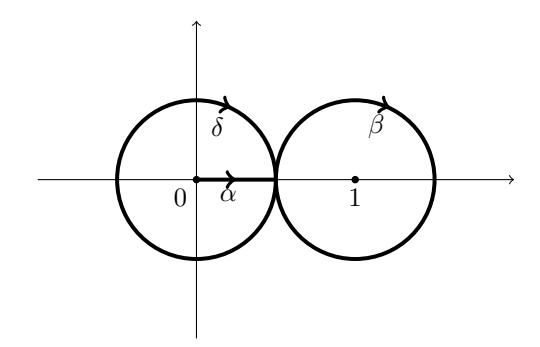
\includegraphics[width=0.6\textwidth]{assets/fig/_page_166_Figure_2.jpeg}
\caption{路径 $\gamma = \alpha^{-1}\beta^{-1}\delta\beta\alpha$.}\label{fig:12.0.7}
\end{figure}

\subsection{纯函数与 Zagier 函数的线性无关性}\label{sec:12.1}

回忆由\rdef{def:11.2.1}：
\[ G(y) = H(x) + H\left(\frac{x}{x-1}\right). \]
我们还设：
\[ G_A(y) = H_A(x) + H_A\left(\frac{x}{x-1}\right) \in \mathbf{Z}[\! [y]\!], \]
它是下面方程 \eqref{eq:12.1.5} 中显式给出的一个 4 阶齐次常微分方程的解。我们最后的函数线性无关性结果如下：

\begin{mylemma}{14 个函数}{lem:12.1.1}
七个函数
\[ \int G(y) dy, \quad \int \frac{G(y) - G(0)}{y} dy, \quad \int \frac{G(y) - G(0) - G'(0)y}{y^2} dy, \]
\[ G(y), \quad G'(y), \quad G''(y), \quad G'''(y), \]
以及这七个函数 $B_i(y)$（对 $i = 1, \dots, 7$），在 $\mathbf{C}(y)$ 上是线性无关的。
\end{mylemma}

\begin{remark}\label{rem:12.1.2}
通过实验来发现\mylem{lem:12.1.1}是相当容易的。一族在 $\mathbf{C}(y)$ 上满足线性关系的幂级数 $A_i(x)$，也在 $\mathbf{C}[y]$ 中满足一个线性关系，因此其系数为次数不超过 $D$ 的多项式（对于某个 $D \in \mathbf{N}_{>0}$）。但是，对于任何给定的 $D$ 是否存在这样的关系，等价于一个显式可计算矩阵的行列式是否消逝。一旦确立了对于中等大小的 $D$（例如 $D = 20$）不存在这样的线性关系，人们就会充分相信该结果是正确的，然后写下证明。我们承认，这正是我们得出\mylem{lem:12.1.1}和引理~14.3.1 的方式，尽管极有可能存在一个能更好地解释这套精密数字的高观点证明。参见\rremark{rem:12.1.12}。\end{remark}

\begin{proof}
由于根据\mylem{lem:12.0.1}，$B_i(y)$ 是线性无关的，任何线性相关关系必定包含至少一个上述带有非零系数的 $G$ 的项。设 $\gamma$ 表示如下路径：首先穿过 $4$，然后穿过 $-1/72$，接着以相反的方向穿过 $4$，最后回到 $0$。函数 $G(y)$ 被替换为 $\widehat{G}(y)$，它是满足与 $G(y)$ 相同的非齐次微分方程的解。另一方面，函数 $\widehat{B}_n(y) = B_n(y)$ 保持不变。由于 $G(y) \neq \widehat{G}(y)$， we 得到了具有相同系数的函数：
\[ \int \widehat{G}(y) \, dy, \quad \int \frac{\widehat{G}(y) - G(0)}{y} \, dy, \quad \int \frac{\widehat{G}(y) - G(0) - G'(0)y}{y^2} \, dy, \]
\[ \widehat{G}(y), \quad \widehat{G}'(y), \quad \widehat{G}''(y), \quad \widehat{G}'''(y) \]
与 $B_i(y)$ 之间的等价线性关系。因此，设 $\Delta = \widehat{G}(y) - G(y)$，我们得到了以下七个函数之间的非零 $\mathbf{C}(y)$-线性关系：
\[ \int \Delta(y) \, dy, \quad \int \frac{\Delta(y)}{y} \, dy, \quad \int \frac{\Delta(y)}{y^2} \, dy, \quad \Delta(y), \quad \Delta'(y), \quad \Delta''(y), \quad \Delta'''(y). \]
但是，$\Delta(y)$ 现在是对应的 4 阶不可约齐次常微分方程（ODE）的解。因此，通过用 $\Delta(y)$ 在单值群 $\pi_1(\mathbf{P}^1 \setminus \{0, -1/72, 4, \infty\})$ 的元素作用下的变换来替换它，我们推导出相应的线性关系必须对任何这样的 $\Delta(y)$ 均成立，特别地，包括全纯解 $\Delta(y) = G_A(y)$。

假设存在这样一个线性关系。在缩放之后，我们可以假设系数位于 $\mathbf{C}(y)$ 中。再次使用求导公式：
\begin{equation}\label{eq:12.1.3}\tag{12.1.3}
\frac{d}{dy} \left\{ A(y) \int F(y) \, dy \right\} = A'(y) \int F(y) \, dy + A(y)F(y).
\end{equation}
在反复求导之后，我们可以假设三个积分项的系数都是常数，并且至少有一个是非零的。因此存在关系：
\begin{equation}\label{eq:12.1.4}\tag{12.1.4}
a_0 \int G_A(y) \, dy + a_{-1} \int \frac{G_A(y)}{y} \, dy + a_{-2} \int \frac{G_A(y)}{y^2} \, dy = \sum_{i=0}^3 b_i(y) G_A^{(i)}(y).
\end{equation}
请注意，我们不能坚持要求 $b_i(y) \in \mathbf{C}[y]$，原因有两个。第一，来自积分的导数项涉及 $G_A(y)$ 除以 $y$ 的幂次。第二，在对 $G_A^{(3)}(y)$ 进行求导时，我们得到了 $G_A^{(4)}(y)$，要将其用较低阶导数 $G_A^{(i)}(y)$ 表达，我们需要除以微分方程中的领先项（leading term）。

实际上，$G_A(y)$ 满足如下常微分方程（ODE）：
\[ \sum_{i=0}^{4} c_i(y) G_A^{(i)}(y) = 0, \]
其中 $c_i(y)$ 定义如下：
\begin{equation}\label{eq:12.1.5}\tag{12.1.5}
\begin{aligned}
c_{0}(y) &= -18(3 + 126y - 712y^{2} + 360y^{3}), \\
c_{1}(y) &= 2(-2 - 2761y + 141632y^{2} - 280328y^{3} + 176412y^{4} - 95616y^{5} + 20736y^{6}), \\
c_{2}(y) &= 2y(-34 - 6353y + 690355y^{2} - 1065613y^{3} + 867876y^{4} - 438336y^{5} + 72576y^{6}), \\
c_{3}(y) &= 2(-4 + y)y^{2}(10 + 204y - 118195y^{2} + 146946y^{3} - 142848y^{4} + 41472y^{5}), \\
c_{4}(y) &= (-4 + y)^{2}y^{3}(1 + 72y)(-1 + 118y - 122y^{2} + 144y^{3}).
\end{aligned}
\end{equation}

因此我们可以假设 $b_i(y) \in \mathbf{C}[y, c_4(y)^{-1}]$。将方程 \eqref{eq:12.1.4} 再进行一次求导，可以得到恒等式：
\begin{equation}\label{eq:12.1.6}\tag{12.1.6}
a_0 G_A(y) + a_{-1} \frac{G_A(y)}{y} + a_{-2} \frac{G_A(y)}{y^2} = \sum_{i=0}^3 \left( b_i'(y) G_A^{(i)}(y) + b_i(y) G_A^{(i+1)}(y) \right).
\end{equation}
我们将 \eqref{eq:12.1.6} 重写为：
\begin{equation}\label{eq:12.1.7}\tag{12.1.7}
\begin{aligned}
a_0 G_{A}(y) + a_{-1} \frac{G_{A}(y)}{y} + a_{-2} \frac{G_{A}(y)}{y^{2}} &= \sum_{i=0}^{3} b'_{i}(y)G_{A}^{(i)}(y) + \sum_{i=1}^{3} b_{i-1}(y)G_{A}^{(i)}(y) + b_{3}(y)G_{A}^{(4)}(y) \\
&= \sum_{i=0}^{3} b'_{i}(y)G_{A}^{(i)}(y) + \sum_{i=1}^{3} b_{i-1}(y)G_{A}^{(i)}(y) - \sum_{i=0}^{3} \frac{c_{i}(y)}{c_{4}(y)}b_{3}(y)G^{(i)}(y),
\end{aligned}
\end{equation}
由此我们推导出联立方程组：
\begin{equation}\label{eq:12.1.8}\tag{12.1.8}
\begin{aligned}
b'_{3}(y) + b_{2}(y) - \frac{c_{3}(y)}{c_{4}(y)}b_{3}(y) &= 0, \\
b'_{2}(y) + b_{1}(y) - \frac{c_{2}(y)}{c_{4}(y)}b_{3}(y) &= 0, \\
b'_{1}(y) + b_{0}(y) - \frac{c_{1}(y)}{c_{4}(y)}b_{3}(y) &= 0, \\
b'_{0}(y) - \frac{c_{0}(y)}{c_{4}(y)}b_{3}(y) &= a_{0} + \frac{a_{-1}}{y} + \frac{a_{-2}}{y^{2}}.
\end{aligned}
\end{equation}

回忆 $b_3(y) \in \mathbf{C}[y, c_4(y)^{-1}]$。此外，给定 $b_3(y)$，人们可以从以下方程归纳地解出 $b_i$（其中 $i \in \{2, 1, 0\}$）：
\[ b_i(y) = \frac{c_{i+1}(y)}{c_4(y)}b_3(y) - b'_{i+1}(y). \]
我们的策略如下：由于 $b_3(y) \in \mathbf{C}(y)$，我们可以考虑 $b_3(y)$ 围绕 $\infty$ 级任意复数点 $\alpha \in \mathbf{C}$ 的幂级数展开。然后，通过考虑最后的等式，我们获得了关于 $b_3(y)$ 在 $\alpha$ 处任意极点阶数的显式边界（请注意，除非 $\alpha = \infty$ 或是 $c_4(y)$ 的根，否则 $b_3(y)$ 将是全纯的）。但这将 $b_3(y)$ 限制为一个有理函数，使得因子 $\operatorname{divisor}(b_3(y)) + D \ge 0$（其中显式除子 $D$ 支撑在 $c_4(y)$ 的根处）。这是一个有限维的（显式可计算的）向量空间，然后我们可以使用线性代数来求解所有可能的 $b_3(y)$。另一种看待这一点的方式是将该系统视为 $b_3(y)$ 的（非齐次）常微分方程，并且我们正在使用 Frobenius 方法计算围绕任意点的（可能）局部展开。显式地，设 $\alpha \neq \infty$，并且
\[ b_3(y) = \sum_{i=N}^{\infty} r_i (y - \alpha)^i, \]
（其中 $N = N_{\alpha}$，$r_i = r_{i,\alpha}$，我们在下面省略了下标），则：
\begin{enumerate}
\item[(1)] 若 $\alpha = 0$，最后的等式变为：
\[ a_0 + \frac{a_{-1}}{y} + \frac{a_{-2}}{y^2} = \frac{-1}{4}(3-N)^2(5-2N)^2r_Ny^{N-4} + \dots \]
\item[(2)] 若 $\alpha = 4$，最后的等式变为：
\[ a_0 + \frac{a_{-1}}{y} + \frac{a_{-2}}{y^2} = \frac{-1}{4}(3-N)(2-N)(5-2N)(3-2N)r_N(y-4)^{N-4} + \dots \]
\item[(3)] 若 $\alpha = -1/72$，最后的等式变为：
\[ a_0 + \frac{a_{-1}}{y} + \frac{a_{-2}}{y^2} = (3 - N)^2 (2 - N)(1 - N)r_N (y + 1/72)^{N-4} + \dots \]
\item[(4)] 若 $\alpha$ 是 $144y^3 - 122y^2 + 118y - 1 = 0$ 的根 $\beta$，则：
\[ a_0 + \frac{a_{-1}}{y} + \frac{a_{-2}}{y^2} = (3 - N)(2 - N)(1 - N)(1 + N)r_N(y - \beta)^{N-4} + \dots \]
\item[(5)] 在 $\alpha \to \infty$ 处，设：
\[ b_3(y) = y^N \sum_{i=N}^{\infty} r_i y^{-i}, \]
我们有：
\[ a_0 + \frac{a_{-1}}{y} + \frac{a_{-2}}{y^2} = \frac{-1}{4}(3-N)^2(5-2N)^2r_Ny^{N-4} + \dots \]
\end{enumerate}

由此我们推导出：
\begin{equation}\label{eq:12.1.9}\tag{12.1.9}
N_{0} \ge 2, \qquad N_{4} \ge 2, \qquad N_{-1/72} \ge 1, \qquad N_{\beta} \ge -1, \qquad N_{\infty} \le 4.
\end{equation}
由此可得：
\begin{equation}\label{eq:12.1.10}\tag{12.1.10}
b_3(y) = \frac{y^2(y-4)^2(y+1/72)}{(144y^3 - 122y^2 + 118y - 1)}Q(y),
\end{equation}
其中 $Q(y)$ 为次数至多为 2 的多项式。然而，如果我们写成：
\[ Q(y) = q_0 + q_1 y + q_2 y^2, \]
那么我们发现：
\begin{equation}\label{eq:12.1.11}\tag{12.1.11}
a_0 + \frac{a_{-1}}{y} + \frac{a_{-2}}{y^2} = \frac{52542464y^{12}q_2 + \dots}{36y^2(-1 + 118y - 122y^2 + 144y^3)^4},
\end{equation}
其中右边的分子是 12 次多项式，其系数关于 $q_0, q_1, q_2$ 是线性的。但现在通过线性代数，人们可以直接检查发现，根本没有参数 $q_i$ 的选择能使分子在分母的非零根处消逝至（至少）一阶。因此，不存在这样的 $b_3(y)$，证明完毕。
\end{proof}

\begin{remark}\label{rem:12.1.12}
假设相反地，我们曾尝试证明这七个函数 $B_i(y)$ 与如下函数之间的（错误的！）线性无关性：
\[
\begin{aligned}
&\int G(y) dy, \quad \int \frac{G(y)-G(0)}{y}dy, \quad \int \frac{G(y)-G(0)-G'(0)y}{y^{2}}dy, \\
&\quad \int \frac{G(y)-G(0)-G'(0)y-G''(0)y^{2}}{y^{3}}dy,
\end{aligned}
\]
\[ G(y), \quad G'(y), \quad G''(y), \quad G'''(y), \]
也就是说，加入另外一个积分。那么论证将完全同上文进行，除了现在我们只能推导出 $N_0 \ge 1$ 而非 $N_0 \ge 2$。然后，写成：
\[ Q(y) = \frac{q_{-1}}{y} + q_0 + q_1 y + q_2 y^2, \]
就像方程 \eqref{eq:12.1.11} 中那样，我们将发现：
\[ a_0 + \frac{a_{-1}}{y} + \frac{a_{-2}}{y^2} + \frac{a_{-3}}{y^3} = \frac{52542464y^{13}q_2 + \dots}{36y^3(-1 + 118y - 122y^2 + 144y^3)^4}. \]
现在，在相差缩放因子意义下，存在唯一的参数 $q_i$ 选择，允许我们消去分子中的单个因子，即（相差常数倍）：
\[ Q(y) = \frac{1}{y} - 278 - 844y - 4644y^{2}. \]
采用来自方程 \eqref{eq:12.1.10} 的这一 $b_3(y)$ 选择，$(144y^3 - 122y^2 + 118y - 1)$ 的幂次完全消失，并且我们到达等式：
\[ a_0 + \frac{a_{-1}}{y} + \frac{a_{-2}}{y^2} + \frac{a_{-3}}{y^3} = \frac{676}{9y^2} + \frac{2}{y^3}. \]
这当然现在有解。这反映了在这些函数之间存在一个线性相关性。事实上，在以下函数之间已经存在一个 $\mathbf{C}(y)$-线性相关性：
\[
\begin{aligned}
& \int \frac{G_A(y)}{y^2} \, dy, \quad \int \frac{G_A(y)}{y^3} \, dy, \quad G_A(y), \\
& \quad G_A'(y), \quad G_A''(y), \quad G_A'''(y) \quad \text{和} \quad 1.
\end{aligned}
\]
作为与解 $a_{-2} = 676/9$ 和 $a_{-3} = 2$ 的另一个相容性检查，我们有（与方程 \eqref{eq:12.1.6} 类比）：
\[ a_0 G_A(y) + a_{-1} \frac{G_A(y)}{y} + a_{-2} \frac{G_A(y)}{y^2} + a_{-3} \frac{G_A(y)}{y^3} = \frac{676}{9} \frac{G_A(y)}{y^2} + 2 \frac{G_A(y)}{y^3} \]
\[ = \frac{4}{y^3} + \frac{866}{9y^2} - \frac{68728}{3} + \dots \]
它不含 $1/y$ 项，这与它是 $y = 0$ 处亚纯函数的导数是一致的。
\end{remark}


% 引入第13节内容
\section{\texorpdfstring{$1, \zeta(2), L(2, \chi_{-3})$}{1, \textbackslash{}zeta(2), L(2, \textbackslash{}chi\_\{-3\})} 的线性无关性证明}\label{sec:13}

在本节中, 我们利用附录 A 的结果来完成定理 A 的证明. 
该证明是通过反证法进行的, 即通过证明某个特定的 G-函数不可能存在来进行. 
假设为了导出矛盾, 在周期 \(1, \zeta(2), L(2, \chi_{-3})\) 之间存在一个 \(\mathbf{Q}\)-线性关系, 
我们可以将其写为:
\begin{equation}\label{eq:13.0.1}
a + b \cdot L(2, \chi_{-3})/2 + c \cdot \zeta(2)/4 = 0
\end{equation}
对于某些不全为零的有理整数 \(a, b, c \in \mathbf{Z}\). 
命题 11.1.8 随后构造了一个具有分母类型 \([1,\dots,n]^2\) 
且在 \(\mathbf{P}^1 \setminus \{0,1/9,1,\infty\}\) 上 holonomic 延拓的特定 G-函数 \(H(x) \in \mathbf{Q}[\![x]\!]\).

现在, 第 11.2 节将该 G-函数 \(H(x)\) 转换为了在对称坐标
\[ y := x + x/(x - 1) = x^2/(x - 1) \]
下的 G-函数 \(G(y) := \operatorname{Sym}^+ H(x) \in \mathbb{Q}[\![y]\!]\). 
引理 11.2.2 表明 \(G(y) \in \mathbf{Q}[\![y]\!]\) 的分母类型为 \([1,\dots,2n]^2\). 
在另一方面, \(G(y)\) 在 \(y \in \mathbf{P}^1 \setminus \{0,4,\infty,-1/72\}\) 上是 holonomic 的, 
在 \(y \in \mathbf{C} \setminus [4,\infty)\) 上是全纯的, 
并且绕 y = 4 具有 \(\mathbf{Z}/2\) 局部单值性.

我们应用定理 6.0.2 于具有如下形式的 \(14 \times 2\) 分母类型数组：
\begin{equation}\label{eq:13.0.2}
\mathbf{b} := \begin{pmatrix} 
0 & 2 & 2 & 2 & 2 & 2 & 2 & 2 & 2 & 2 & \dots \\ 
0 & 0 & 2 & 4 & 4 & 4 & 4 & 4 & 4 & 4 & \dots
\end{pmatrix}^{\mathrm{t}}
\end{equation}
以及增加积分向量：
\[ \mathbf{e} := (0, 0, 1; 0, 0, 0, 0, 0, 0; 1, 1, 1, 1, 1), \]
该定理是在将等式中的字母 x 替换为轴对称化字母
\[ y := x + x/(x-1) = x^2/(x-1) \]
以及取以下有序函数列表 \(\{f_i\}_{i=1}^{14}\) （参见 (10.1.2), (10.1.4) 以及 (10.2.1)）的前提下浮现的:
\[ B_1(y), B_2(y), B_3(y); B_4(y), B_5(y), G(y), G'(y), G''(y), G'''(y); \]
\[ B_6(y), B_7(y), \int G(y) dy, \int \frac{G(y) - G(0)}{y} dy, \int \frac{G(y) - G(0) - G'(0)y}{y^2} dy. \]
这 14 个函数的 \(\mathbf{Q}(y)\)-线性无关性已经在引理 12.1.1 中得到证明. 
它们的分母类型已在引理 10.2.2 中被计算出来. 
对于这些积分, 我们评述：由除以 y 的方幂而引起的索引移动意味着这些函数在字面上不具有分母类型 \(n[1, 2, \ldots, 2n]^2\), 
而实际上具有分母类型 \(n[1, 2, \ldots, 2n + 3]^2\)； 
由于注记 6.0.12, 这并不是一个问题.

我们用 \(\mathcal{H}_{Y_0(2)}\) 表示由这些函数组成的 14-维 \(\mathbf{Q}(y)\)-线性生成空间. 
对于在已发展的各种 holonomy 边界中浮现的解析映射 \(\varphi\), 
我们取引理 A.4.4 中全纯映射 \(\varphi \in \mathcal{O}(\overline{\mathbf{D}})\) 的限制 \(\varphi(rz)\). 
由 \(\Sigma^0_{Y_0(2)} := \{-1/72\}\), \(\Sigma^1_{Y_0(2)} := \emptyset\), \(\varphi_{Y_0(2)} := \varphi\) 
以及为线段 [-1/72, 0] 的一个足够小的开邻域的 \(U_{Y_0(2)}\) 下使用的推论 9.0.19, 
我们拥有解析性 \(\varphi^*\mathcal{H}_{Y_0(2)} \subset \mathcal{M}(\overline{\mathbf{D}})\).

\begin{figure}[!htbp]
  \centering
  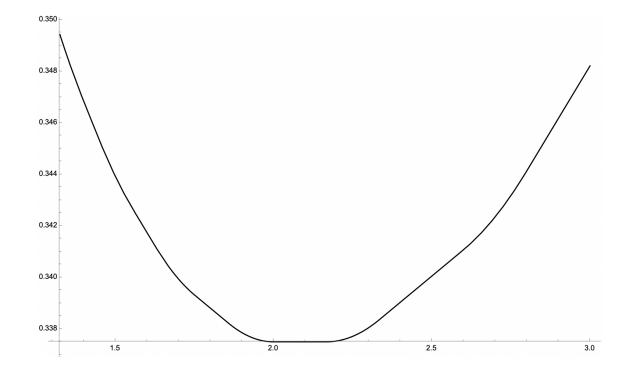
\includegraphics[width=0.45\textwidth]{assets/fig/_page_171_Figure_13.jpeg}
  \caption{\(\xi \in [1.325, 3]\) 范围内 \((6\xi + I_{\xi}^{14}(\xi))/98\) 的函数图像片段，显示区间 \(\xi \in [2, 13/6]\) 为恒定的极小值点.}\label{fig:13.0.3}
\end{figure}

对分母速率, 我们计算出:
\begin{equation}\label{eq:13.0.4}
\tau^{\flat}(\mathbf{b}) = \frac{1 \cdot 0 + (3+5) \cdot 2 + (7+9+11+13+\dots+27) \cdot 4}{14^2} = \frac{191}{49}
\end{equation}
并且, 由图~\ref{fig:13.0.3}（其揭示了 \(\xi \in [2, 13/6]\) 是一致的极大值点）:

\begin{equation}\label{eq:13.0.5}
\begin{aligned}
\tau^{\sharp}(\mathbf{e}) 
&= \frac{2}{m^{2}} \min_{\xi \in [0, m]} \left\{ \xi \sum_{i=1}^{m} e_{i} + \left( \max_{1 \le i \le m} e_{i} \right) I_{\xi}^{m}(\xi) \right\} \\
&= \min_{\xi \in [0, 14]} \left\{ \frac{6\xi + I_{\xi}^{14}(\xi)}{98} \right\} \\
&= \frac{12 + I_{2}^{14}(2)}{98} = \frac{27}{80}.
\end{aligned}
\end{equation}
我们获得:
\begin{equation}\label{eq:13.0.6}
\tau(\mathbf{b}; \mathbf{e}) = \tau^{\flat}(\mathbf{b}) + \tau^{\sharp}(\mathbf{e}) = \frac{191}{49} + \frac{27}{80} = \frac{16603}{3920} = 4.235459...
\end{equation}
这正是在公式 (A.5.1) 中浮现的数值 \(\frac{191}{49} + \frac{27}{80} = \frac{16603}{3920}\).

我们现在可以与我们的 holonomy 边界建立联系来证明定理 A. 
根据命题 11.1.8 以及引理 12.1.1, 
在假设存在 \(\mathbf{Q}\)-线性关系 \eqref{eq:13.0.1} 的前提下, 
我们拥有一组具有分母类型 \eqref{eq:13.0.2} 且在 \(\mathbf{Q}[y]\) 中在 \(\mathbf{Q}(y)\) 上线性无关的 m = 14 个（holonomic）函数. 
因此, 只要证明我们的任何一个 holonomy 边界均给出 m < 14, 就足以反驳 \eqref{eq:13.0.1}.

例如：

\begin{proof}[基于定理 7.0.1 的证明]
应用定理 7.0.1, 我们获得了上界 \(m \le 13.9938...\), 这正是公式 (A.5.1) 中计算出的.
\end{proof}

\begin{proof}[基于定理 6.0.2 的证明]
应用具有 \(l=1, r_0=e^{-1/2}, \gamma_1=14\) 的定理 6.0.2. 
由在引理 7.6.8 中类似的数值理由, 我们选取这一特定的参数. 
在此情况下, 我们有:
\[ \int_0^1 2t \cdot g_{\varphi, \gamma}^*(t) \, dt = 11.316 \dots \]
并且因此, holonomy 边界读作:
\[ m \le \frac{11.316... + \frac{1}{14} \cdot 2.926^2 \cdot \frac{1}{2}}{\log\left(256 \cdot \frac{5448339453535586608000000000}{8658833407565631122430056127}\right) - \left(\frac{27}{80} + \frac{191}{49}\right)} = 13.730... < 14. \]
\end{proof}

\begin{proof}[基于定理 7.1.6 的证明]
伴随如示例 7.4.6 中取 \(r_0 = e^{-1/2}\) 以及 \(r_1 = 1\) 的参数选择, 我们获得了边界（参见等式 (7.4.7)）.
\end{proof}

当然, 我们也可以应用第 7 节中的其他 holonomicity 边界. 
参见具有四个半径 \(r_i\) 而非两个的示例 7.4.6, 以及示例 7.5.9 以及 7.6.8.

\begin{remark}\label{rem:13.0.7}
如果我们一直坚持处于没有增加积分的、定理 2.5.1 的更粗糙框架 \(\mathbf{e} = \mathbf{0}\) 下, 
我们将不得不把 \(\mathbf{b}\) 扩充为数组:
\begin{equation}\label{eq:13.0.8}
\mathbf{b}' := \begin{pmatrix} 
0 & 2 & 2 & 2 & 2 & 2 & 2 & 2 & 2 & 2 & \dots \\ 
0 & 0 & 2 & 4 & 4 & 4 & 4 & 4 & 4 & 4 & \dots \\
0 & 0 & 0 & 0 & 0 & 0 & 0 & 0 & 2 & 2 & \dots
\end{pmatrix}^{\mathrm{t}}
\end{equation}
注意，尽管该 \(\mathbf{b}'\) 在字面上不具有定理 6.0.2 中的特定形式, 
但我们可以应用定理 8.0.1 中更一般的分母公式 \eqref{eq:8.0.2}. 
然而, 为了简单起见, 我们给出了关于 \(\tau^{\flat}(\mathbf{b}')\) 的一个足够优秀的估计, 
这足以说明引入非零 \(\mathbf{e}\) 的必要性. 
在一方面, 注记 8.0.6 中的上界论证适用于其中每一列都具有两个值（包括其中一个是 0）的那些 \(\mathbf{b}'\). 
因此我们有 \(\tau^{\flat}(\mathbf{b}') \leq (2+2+1) - \frac{1}{14^2}(1^2 \cdot 2 + 3^2 \cdot 2 + 8^2 \cdot 1) = \frac{32}{7} = 4.571...\)

在另一方面, 根据 \eqref{eq:8.0.2} 的定义, 
通过仅考虑满足 \(n_{j_1} > n_{j_2} \implies i_{j_1} \ge i_{j_2}\) 的 \(\mathbf{n}\), 我们有一个容易的下界, 
并且有 \(\tau^{\flat\flat}(\mathbf{b}')\) 至少为:
\[
\begin{aligned}
&\frac{1}{14^2} \Big( 1 \cdot 0 + 3 \cdot 2 + 5 \cdot (2 + 1) + (7 + 9 + \dots + 17) \cdot (2 + 2) \\
&\quad + (19 + 21 + 23 + 25 + 27) \cdot (2 + 2 + 1) \Big)
\end{aligned}
\]
\[ = \frac{884}{196} = 4.510\dots, \]
这是一个相比于 \eqref{eq:13.0.6} 明显更差的数值. \end{remark}

% 引入第14节内容
\section{两个对数的乘积}\label{sec:14}

在本节中, 我们将我们的方法应用到某些对数的乘积上. 
Baker 定理 \cite{Bak64} 给出了关于对数线性形式的决定性结果（甚至是在 \(\overline{\mathbf{Q}}\) 上）, 
但我们仍然不知道如何证明 \(\log 2 \cdot \log 3\) 以及 \(\pi \cdot \log 2\) 是无理数. 
虽然我们的方法（目前！）同样无法处理那些情况, 但我们确实证明了定理 C, 我们在此再次予以回顾：

\begin{theorem}\label{thm:14.0.1}
设 \(m, n \in \mathbf{Z} \setminus \{-1, 0\}\) 是满足 \(\left| \frac{m}{n} - 1 \right| < \frac{1}{10^6}\) 的有理整数. 
那么
\begin{equation}\label{eq:14.0.2}
\log\left(1 + \frac{1}{m}\right)\log\left(1 + \frac{1}{n}\right)
\end{equation}
是无理数. 
此外, 当 \(m \neq n\) 时, 以下四个数在 \(\mathbf{Q}\) 上是线性无关的:
\begin{equation}\label{eq:14.0.3}
1, \quad \log\left(1+\frac{1}{m}\right), \quad \log\left(1+\frac{1}{n}\right), \quad \log\left(1+\frac{1}{m}\right)\log\left(1+\frac{1}{n}\right).
\end{equation}
\end{theorem}

\begin{remark}\label{rem:14.0.4}
我们当然可以通过我们的方法改进常数 \(10^{-6}\), 
但一些计算表明, 人们不太可能做得到比（比如） \(10^{-4}\) 更好的结果, 
以及可能根本无法达到那么远；我们选择这个常数是为了其相对简单性. \end{remark}

\(m=n\) 的退化情况是 \(\mathbf{Q} \setminus \{1\}\) 中有理数 r 的 \(\log r\) 超越性的平凡推论, 
因此我们将假设 \(m \neq n\). 
我们首先召回关于
\begin{equation}\label{eq:14.0.5}
\log\left(1 + \frac{1}{m}\right)
\end{equation}
对于 \(m \geq 1\) 的无理性的一个证明（源于 \cite{AR80}\cite{Chu79}\cite{vdP79}）, 该证明基于 Ap{\'e}ry 极限方法. 
这与我们在基本注记 2.10.1 中叙述的构造以及在第 3.3.7 节中关于对数函数的 Hermite--Pad{\'e} 构造是密切相关的.

设 a > 1 是一个有理整数. 函数
\begin{equation}\label{eq:14.0.6}
A(a,x) := \frac{1}{\sqrt{1 - 2ax + x^2}} = \sum_{n=0}^{\infty} u_n(a)x^n
\end{equation}
当 a 是奇数时属于 \(\mathbf{Z}[x]\), 否则属于 \(\mathbf{Z}[x/2]\), 
并且满足一阶线性 ODE:
\begin{equation}\label{eq:14.0.7}
(1 - 2ax + x^2)y' + (x - a)y = 0.
\end{equation}
存在唯一的有理系数全纯非齐次 ODE
\[ (1 - 2ax + x^2)y' + (x - a)y = 1 \]
的在 0 处消逝的全纯解；它由下式给出:
\begin{equation}\label{eq:14.0.8}
H(a,x) := \frac{1}{\sqrt{1 - 2ax + x^2}} \int_0^x \frac{dt}{\sqrt{1 - 2at + t^2}}
\end{equation}
\[ = \frac{1}{\sqrt{1 - 2ax + x^2}} \left( \log\left(a - x - \sqrt{1 - 2ax + x^2}\right) - \log(a - 1) \right) \]
\[ = x + \frac{ax^2}{2} + \frac{(3a^2 - 1)x^3}{6} + \dots = \sum_{n=0}^{\infty} v_n(a)x^n \in \mathbf{Q}[x], \]
并且此外, 它的系数 \(v_n(a)\) 当 a 是奇数时满足 \([1, 2, \ldots, n]v_n(a) \in \mathbf{Z}\), 
否则满足 \([1, 2, \ldots, n]2^n v_n(a) \in \mathbf{Z}\). 
根据 \eqref{eq:14.0.8}, 我们有公式:
\[ H(a,x) - \frac{1}{2}\log\left(\frac{a+1}{a-1}\right)A(a,x) = \frac{1}{\sqrt{1-2ax+x^2}} \int_{a-\sqrt{a^2-1}}^{x} \frac{dt}{\sqrt{1-2at+t^2}} \]
其右手边由于在沿着包围该奇点 \(x=a-\sqrt{a^2-1}\) 
的简单回路进行解析延拓后两个因子的相乘 \((-1)\) 单值性而在该奇点处超收敛. 
这与第 2.11.12 节中关于超收敛的机制以及在第 11.1 节中关于 Eisenstein 级数 A 以及 Eichler 积分 \(B-\frac{1}{2}L(2,\chi_{-3})\) 的消去模形式权重的机制是完全相同的. 
当前研究的情况很容易被看出：在不改变记号的前提下, 
等价于由对数函数的对角 Hermite--Pad{\'e} 逼近表产生的一阶线性 ODE \eqref{eq:3.3.12} 以及公式 \eqref{eq:3.3.8}, 
这我们在第 3.3.7 以及 3.3.13 节中已经叙述过.

紧接着有:
\begin{equation}\label{eq:14.0.9}
\lim_{n \to \infty} \frac{v_n(a)}{u_n(a)} \to \frac{1}{2} \log \left( \frac{a+1}{a-1} \right)
\end{equation}
收敛得足够快, 以便在不等式:
\[ 5.828... = 3 + 2\sqrt{2} > e = 2.718..., \]
\[ 7.872... = 4 + \sqrt{15} > 2 \cdot e = 5.43656... \]
的前提下证明对于任意奇数 \(a \geq 3\) 以及任意偶数 \(a \geq 4\) 这一数量的无理性. 
如果设 a = 1 + 2m, 那么有
\[ \log\left(\frac{a+1}{a-1}\right) = \log\left(1 + \frac{1}{m}\right), \]
并随之如所期望的那样给出了数量 \eqref{eq:14.0.5} 的无理性（其通过对该论证 of 较好研究, 被 Chudnovsky \cite{Chu79}\cite{Chu83b} 进一步精细化为了相当卓越的无理数测度）.

我们现在考虑数量:
\begin{equation}\label{eq:14.0.10}
\log\left(\frac{a+1}{a-1}\right)\log\left(\frac{b+1}{b-1}\right)
\end{equation}
对于一对不同的有理整数 \(a \neq b\) 的算术性质. 
由 \eqref{eq:14.0.9} 显然有:
\begin{equation}\label{eq:14.0.11}
\lim_{n \to \infty} \frac{v_n(a)}{u_n(a)} \cdot \frac{v_n(b)}{u_n(b)} \to \frac{1}{4} \log\left(\frac{a+1}{a-1}\right) \log\left(\frac{b+1}{b-1}\right).
\end{equation}
然而, 这一收敛显然无法通过任何初等分析快到足以证明右手边的无理性. 
我们仍然将会看到：只要 a/b 足够接近 1, 
这一数量就可以通过我们基于底层生成级数的函数论性质以及 Hadamard 乘积运算（它允许构造具有所需 Ap{\'e}ry 极限的新 G-函数）的基本性质的全新方法来接近.

对于每一对整数 a, b \(\in \mathbf{Z} \setminus \{-1, 0, 1\}\), 让我们写出:
\[ \eta_a := \frac{1}{2} \log \left( \frac{a+1}{a-1} \right), \quad \eta_b := \frac{1}{2} \log \left( \frac{b+1}{b-1} \right), \]
\[ \eta_{a,b} := \eta_a \eta_b := \frac{1}{4} \log \left( \frac{a+1}{a-1} \right) \log \left( \frac{b+1}{b-1} \right). \]
我们将假设 \(a \neq \pm b\), 因为 \(\eta_{a,a} = -\eta_{a,-a} = \eta_a^2\) 的无理性以及超越性已经是已知的. 
我们对于周期乘积 \(\eta_{a,b} = \eta_a \eta_b\) 算术性质的研究途径是通过底层 G-函数的 Hadamard 乘积进行的.

\subsection{Hadamard 乘积以及 Ap{\'e}ry 极限}\label{sec:14.1}

设 \(\star\) 表示在幂级数上的 Hadamard 乘积运算：\((\sum a_n x^n) \star (\sum b_n x^n) := \sum a_n b_n x^n\). 
函数
\begin{equation}\label{eq:14.1.1}
P_A(x) := A(a, x) \star A(b, x) = \sum u_n(a)u_n(b)x^n
\end{equation}
满足以下形式的一阶线性 ODE \(\mathcal{M}(P_A(x)) = 0\):
\begin{equation}\label{eq:14.1.2}
(-1+x)x(1+x)(1-4abx-2x^2+4a^2x^2+4b^2x^2-4abx^3+x^4)y''
\end{equation}
\[ +(-1+8abx+5x^2-12a^2x^2-12b^2x^2+16abx^3-7x^4+4a^2x^4+4b^2x^4-8abx^5+3x^6)y' \]
\[ +(ab-(-1+3a^2+3b^2)x+8abx^2-(2+a^2+b^2)x^3-abx^4+x^5)y=0. \]
点 x = 1 以及 x = -1 是该 ODE 的表观奇异点, 
只要分别满足 \(a-b \neq 0\) 以及 \(a+b \neq 0\). 
这既根据 Hadamard 乘积的一般性质 \cite{Her1893} 成立, 
也可以直接通过计算指标方程（为 \(R(R-2)=0\)）以及确立存在两个线性无关的幂级数解来予以验证. 
例如, 对于推定解 \(\sum c_n(x+1)^n\), 系数满足如下递推关系:
\[ (a+b)^2 n(n-2)c_n = 12(a+b)^2 c_{n-1} - 4(a+b)^2 (n-2) c_{n-1} (7n-9)(n-2) + 6(a+b)^2 c_{n-2} + (n-2) c_{n-2}(\ldots) + \dots, \]
这蕴含了存在至少一个具有形式 \(x^2 + \dots\) 的解, 
但还存在另一个具有如下形式的解:
\[ 1 + \frac{(x+1)}{2} - \frac{(x+1)^3}{4} + \dots \in \mathbf{Q}[a, b, x+1]. \]
对于 x = 1 的情况也是完全类似的. 
四阶多项式的四个根恰好是各一阶 ODE 奇异点的乘积, 
即:
\[ \left(a\pm\sqrt{a^2-1}\right) \left(b\pm\sqrt{b^2-1}\right). \]

\begin{remark}[Basic Remark 14.1.3]\label{rem:14.1.3}
如果 a 以及 b 很大且 a/b 以及接近 1, 
那么 \eqref{eq:14.1.2} 的四个非零有限奇异点分组如下:
\begin{itemize}
  \item[(1)] 一个奇异点 \(\alpha\) 以及接近 0.
  \item[(2)] 两个奇异点以及接近 1.
  \item[(3)] 一个以及巨大的奇异点（“接近 \(\infty\)”）.
\end{itemize}
除了这些之外, 0 以及 \(\infty\) 自身也是（本质）奇异点. 
我们将在假设量 \eqref{eq:14.0.3} 在 \(\mathbf{Q}\) 上线性相关的条件下, 
构造一个具有分母类型 \(\tau = [1,2,\dots,n]^2\) 
且满足 \eqref{eq:14.1.2} 的非齐次版本、并在 \(\alpha\) 之外超收敛的有理系数函数 \(H(x)\). 
当在 \(\mathbf{P}^1 \setminus \{0,1,\infty\}\) 上研究具有分母类型 \(\tau = [1,2,\dots,n]^2\) 
的函数时, 根据第 2.9.5 节, 我们被要求选择一个满足 \(\varphi(0)=0\) 以及 \(\varphi^{-1}(0)=\{0\}\) 
的辅助全纯映射 \(\varphi: \mathbf{D} \to \mathbf{C} \setminus \{1\}\). 
如果我们限制 \(\varphi\) 到对于任意 \(\epsilon \in (0,1/2]\) 的圆盘 \(D(0,1-\epsilon)\) 上, 
那么 \(\varphi\) 的值域将避开包含 1 的一个微小开球以及包含 \(\infty\) 的一个开球, 
并满足 \(\#\varphi^{-1}(\alpha)=1\). 
这正是我们的 holonomy 边界可以被应用的设定, 
因为我们不仅可以纳入形式函数 \(H(x)\) 以及它们的导数, 
还可以纳入我们在第 10 节中设计的、在 \(\mathbf{P}^1 \setminus \{0,1,\infty\}\) 上的纯函数. 
在实际中, 我们的映射 \(\varphi\) 具有 \(\lambda \circ \psi\) 的形式, 
或者在等价的 \(\mathbf{P}^1 \setminus \{0,4,\infty\}\) 设定下, 具有 \(h \circ \psi\) 的形式, 
其中 \(\psi : \overline{\mathbf{D}} \to \mathbf{D}\) 
是我们在 \(\mathbf{D}\) 内一合适选择区域的 Riemann 映射. 
但是, 尽管函数 \(\lambda\) 排除了在 \(\mathbf{D}\) 上的 1, 
但为了排除与 1 相差 \(\epsilon\) 以内的值, 
就需要 \(\psi\) 具有明显更小的共形半径, 
除非 \(\epsilon\) 是以及微小的. 
例如, 如果 \(\psi(\mathbf{D})\) 在 \(\mathbf{D}\) 内的像包含了点 3/4, 
那么在 \(\mathbf{D}\) 上的 \(\varphi = \lambda \circ \psi\) 
将已经包含了值:
\[ \lambda(3/4) = 0.9999999999999999332\dots \]
这一数值特征是最终迫使我们要假设 \(|m/n-1|\) 是以及微小的值的原因. \end{remark}

\subsubsection{超收敛空间}\label{sec:14.1.4}

我们现在考虑对乘积 ODE \eqref{eq:14.1.2} 的非齐次形式的解. 
用 \(\mathcal{M}\) 表示 \eqref{eq:14.1.2} 的对应微分算子, 
那么我们也有以下恒等式:
\[ \mathcal{M}(H(a,x) \star A(b,x)) = -b + 3ax - 3bx^{2} + ax^{3}, \]
\[ \mathcal{M}(A(a,x) \star H(b,x)) = -a + 3bx - 3ax^{2} + bx^{3}, \]
\[ \mathcal{M}(H(a,x) \star H(b,x)) = -1 + 2x^{2} - x^{4}. \]
我们进一步声称, 函数:
\begin{equation}\label{eq:14.1.5}
P_{a} := (H(a,x) - \eta_{a}A(a,x)) \star A(b,x) = \sum (v_{n}(a) - \eta_{a}u_{n}(a))u_{n}(b)x^{n},
\end{equation}
\[ P_{b} := A(a,x) \star (H(b,x) - \eta_{b}A(b,x)) = \sum u_{n}(a)(v_{n}(b) - \eta_{b}u_{n}(b))x^{n}, \]
\[ P_{ab} := H(a,x) \star H(b,x) - \eta_{a,b}A(a,x) \star A(b,x) = \sum (v_{n}(a)v_{n}(b) - \eta_{a,b}u_{n}(a)u_{n}(b))x^{n} \]
\[
\begin{aligned}
&= \sum \left( \eta_{a}u_{n}(a)(v_{n}(b) - \eta_{b}u_{n}(b)) + \eta_{b}(v_{n}(a) - \eta_{a}u_{n}(a))u_{n}(b) \right) x^{n} \\
&\quad + \sum (v_{n}(a) - \eta_{a}u_{n}(a))(v_{n}(b) - \eta_{b}u_{n}(b))x^{n}
\end{aligned}
\]
是超越了最小奇异点 \((a - \sqrt{a^2 - 1})(b - \sqrt{b^2 - 1})\) 之外超收敛的. 
这根据以下估计而成立:
\[ |v_n(a) - \eta_a u_n(a)| = O((a - \sqrt{a^2 - 1})^{n(1 - \epsilon)}), \]
\[ |v_n(b) - \eta_b u_n(b)| = O((b - \sqrt{b^2 - 1})^{n(1 - \epsilon)}), \]
伴随着:
\[ |v_n(a)|, |u_n(a)| = O((a + \sqrt{a^2 - 1})^{n(1+\epsilon)}), \]
\[ |v_n(b)|, |u_n(b)| = O((b + \sqrt{b^2 - 1})^{n(1+\epsilon)}). \]

我们可以将 \(P_{ab}\) 在 \eqref{eq:14.1.5} 最后两行中的级数分解写为以下等同形式:
\[
\begin{aligned}
P_{ab} &= \eta_a A(a, x) \star (H(b, x) - \eta_b A(b, x)) + \eta_b (H(a, x) - \eta_a A(a, x)) \star A(b, x) \\
&\quad + (H(a, x) - \eta_a A(a, x)) \star (H(b, x) - \eta_b A(b, x)).
\end{aligned}
\]
我们在此处利用的一般事实 \cite{Her1893} 是：任意一组 holonomic 幂级数的 Hadamard 乘积仍然是超收敛的, 
只要其中至少有一个是第 2.9 节意义下的超收敛分支. 
这在本质上与 Jacobson 恒等式 \(1-xy=(1-x)+(1-y)-(1-x)(1-y)\) 结合在了一起, 
后者例如在有限 p-群的 \(\mathbf{F}_p\)-群环的增广理想的幂零性证明中是熟知的.

\subsubsection{不可能的 G-函数的构造}\label{sec:14.1.6}

假设现在直到定理 14.0.1 证明的末尾, 
都存在不全为零的整数 \(r_0, r_a, r_b\) 以及 \(r_{ab}\), 使得:
\begin{equation}\label{eq:14.1.7}
r_a \eta_a + r_b \eta_b + r_{ab} \eta_{a,b} = r_0.
\end{equation}
那么线性组合
\begin{equation}\label{eq:14.1.8}
P := r_{a}P_{a} + r_{b}P_{b} + r_{ab}P_{ab} = r_{a}H(a, x) \star A(b, x) + r_{b}A(a, x) \star H(b, x) + r_{ab}H(a, x) \star H(b, x) + r_{0}A(a, x) \star A(b, x)
\end{equation}
\[ = \sum c_{n}(a, b)x^{n} \in \mathbf{Q}[\![x]\!] \]
也属于第 14.1.4 节中的超收敛空间, 
但现在它具有有理数系数. 
这就是依赖于我们关于线性相关性 \eqref{eq:14.1.7} 的荒谬假设、而将最终被我们的 holonomy 边界反驳的该 G-函数. 
该不可能函数的解析性质源于第 14.1.4 节中的超收敛性；我们现在收集其算术性质. 
如果 a 以及 b 都是奇数, 那么 \(u_n(a), u_n(b) \in \mathbf{Z}\) 
并且此外 \([1, 2, \ldots, n]v_n(a)\) 以及 \([1, 2, \ldots, n]v_n(b)\) 都在 \(\mathbf{Z}\) 中. 
因此, 在 Hadamard 乘积构造下:
\[ [1, 2, \dots, n]^2 c_n(a, b) \in \mathbf{Z}. \]
此外, 伴随 a=1+2m 以及 b=1+2n, 线性关系 \eqref{eq:14.1.7} 的不存在性恰好是定理 C 的结论. 
（条件 \(a,b\in \mathbf{Z}\setminus \{-1,0,1\}\) 变为了 \(m,n\in \mathbf{Z}\setminus \{-1,0\}\).） 
因此, 为了证明定理 C, 只要假设存在关系 \eqref{eq:14.1.7} 以及如 \eqref{eq:14.1.8} 中的函数 P(x), 
并确立一个矛盾即为足够.

\begin{definition}\label{def:14.1.9}
在 \(r_a, r_b\) 以及 \(r_{ab}\) 满足 \eqref{eq:14.1.7} 的前提下, 
设 P(x) 如等式 \eqref{eq:14.1.8} 中定义, 并且设:
\[ G(y) := P(x) + P\left(\frac{x}{x-1}\right) \in \mathbf{Q}[\![y]\!]. \]
伴随如 \eqref{eq:14.1.1} 的 \(P_A(x) = A(a, x) \star A(b, x)\), 设:
\[ G_A(y) := P_A(x) + P_A\left(\frac{x}{x-1}\right), \]
并因此当 a, b 是奇数时有 \(G_A(y) \in \mathbf{Z}[\![y]\!]\), 否则有 \(G_A(y) \in \mathbf{Z}[\![1/2]\!][\![y]\!]\). \(\vartriangle\)
\end{definition}

与定理 A 的证明以及相似, 我们将在第 9 节的字典中研究 \(Y_0(2)\) 情况, 
以及反驳存在具有分母类型 \([1, \ldots, 2n]^2\) 
以及“接近于”我们在第 10 节中研究的 \(\mathbf{P}^1 \setminus \{0, 4, \infty\}\) 类型的 G-函数 \(G \in \mathbf{Q}[\![y]\!]\). 
我们在下文命题 14.1.11 中记录 G 的这些性质, 在此之前首先给出以下定义:

\begin{definition}\label{def:14.1.10}
令 \(y_{a^{\pm},b^{\pm}}\) 表示由下式给出的 \(y:=\pi(x)=x+\frac{x}{x-1}\) 的像:
\[ x = \left(a \pm \sqrt{a^2 - 1}\right) \left(b \pm \sqrt{b^2 - 1}\right), \]
其中考虑了所有四个符号对. 用 \(\mathcal{L}\) 表示 \(\mathcal{M}\) 在 \(\pi\) 下的推前, 
从而满足 \(\mathcal{L}(G_A(y)) = 0\). \(\vartriangle\)
\end{definition}

我们当前的讨论是有条件地建立在假设 \(\mathbf{Z}\)-线性关系 \eqref{eq:14.1.7} 成立的前提下的. 
在此处, 我们做出额外的假设：有理整数 \(a, b \in \mathbf{Z} \setminus \{\pm 1\}\) 是奇数.

\begin{proposition}\label{prop:14.1.11}
对于奇数 \(a, b \in \mathbf{Z} \setminus \{\pm 1\}\), 
第 14.1.9 节中定义的函数 \(G(y) \in \mathbf{Q}[\![y]\!]\) 以及 \(G_A(y) \in \mathbf{Q}[\![y]\!]\) 
分别具有分母类型 \([1, \ldots, 2n]^2\) 以及 1. 
此外, \(\mathcal{L}(G_A(y)) = 0\) 并且对于 \(\mathbf{Q}(y)\) 上的某个非零线性微分算子 \(\mathcal{L}\) 
有 \(\mathcal{L}(G(y)) \in \mathbf{Q}[\![y]\!]\), 该算子满足:
\begin{itemize}
  \item[(1)] \(\mathcal{L}\) 除了 \(y \in \{0, 4, y_{a^{\pm}, b^{\pm}}, \infty\}\) 之外没有别的奇异点.
  \item[(2)] \(\mathcal{L}\) 绕奇异点 y=4 具有 \(\mathbb{Z}/2\) 局部单值性.
\end{itemize}
\end{proposition}

我们将在下文第 14.2 节中显式地写出 \(\mathcal{L}\)； 
多项式 \(\mathcal{L}(G(y)) \in \mathbf{Q}[a, b, y]\) 的确切形式可以被计算出来, 但这并不重要.

\subsection{微分方程 \(\mathcal{L}(G_A) = 0\)}\label{sec:14.2}

在给出引理 14.3.1（引理 12.1.1 的对应物）的表述以及证明之前, 
我们应该更详细地检验 ODE \(\mathcal{L}(G_A) = 0\). 
由于该计算的长度, 与在证明引理 12.1.1 期间证明有关 Zagier 函数的相关事实相比, 
将该计算单独陈述、而不是与引理 14.3.1 的证明交织在一起是更有道理的. 
然而, 读者可能以及希望提前看看引理 14.3.1 的表述, 
以了解我们要往何处去. 
我们从 \eqref{eq:14.1.2} 计算出 \(\mathcal{L}\) 的以下显式形式:
\[ \mathcal{L}(G_A) = \sum_{i=0}^{4} c_i(y) G_A^{(i)}(y) = 0, \]
其中 \(c_i(y)\) 是满足下式的某些多项式:
\begin{equation}\label{eq:14.2.1}
c_{0}(y) = R_{12}(y), \qquad c_{1}(y) = R_{16,A}(y), \qquad c_{2}(y) = yR_{16,B}(y),
\end{equation}
\[ c_{3}(y) = y^{2}(y - 4)R_{15}(y), \qquad c_{4}(y) = (y - 4)^{2}y^{3}R_{4}(y)R_{10}(y). \]
在此, \(R_d(y)\) 表示 \(\mathbf{Q}(a, b, y)\) 中关于 y 的次数为 d 的不可约多项式, 
并且下标 A 以及 B 表示 \(R_{16,A}\) 以及 \(R_{16,B}\) 是不同的. 
多项式
\[ (1-x)^4 R_4 \left(x + \frac{x}{x-1}\right) \]
具有 \((a\pm \sqrt{a^2 - 1})(b\pm \sqrt{b^2 - 1})\) 作为其 8 个根之中的 4 个, 
以及这些根在对合自同构 \(w(x) = x/(x-1)\) 下的像. 
特别地, \(R_4(y)\) 的根是 \(\mathcal{L}\) 的奇异点 \(y_{a^{\pm},b^{\pm}}\). 
多项式 \(R_4(y)\) 以及由下式显式地给出:
\[ R_4(y) = 1 + 4y - 8a^2y - 4aby - 8b^2y + 16a^2b^2y + 4y^2 - 12a^2y^2 + 16a^4y^2 \]
\[ + 20aby^2 - 16a^3by^2 - 12b^2y^2 - 16ab^3y^2 + 16b^4y^2 - 8a^2y^3 + 16aby^3 \]
\[ - 16a^3by^3 - 8b^2y^3 + 32a^2b^2y^3 - 16ab^3y^3 + 4a^2y^4 - 8aby^4 + 4b^2y^4. \]
与 \(R_4(y)\) 以及在 \eqref{eq:14.2.1} 的 \(c_4(y)\) 中出现的 y 以及 \((y-4)\) 
的伴随方幂不同, \(R_{10}(y)\) 的根并不是 \(\mathcal{L}\) 的真实奇异点. 
更确切地, 只要 \(R_{10}(y)\) 的根与 \(R_4(y)y(y-4)\) 的根是两两不同的, 这一结论就是成立的, 
且在我们的假设下, 这根据下文证明的引理 14.2.6 以及 14.2.4 是满足的. 
多项式 \(R_{10}(y)\) 也可被显式地计算出来:
\[ R_{10}(y) = 4a^2b^2 + 9y - 27a^2y - 102aby + 144a^3by - 27b^2y + 207a^2b^2y - 128a^4b^2y \]
\[ + 144ab^3y - 160a^3b^3y - 128a^2b^4y + 64y^2 - 93a^2y^2 + 228a^4y^2 - 284aby^2 + 740a^3by^2 \]
\[ - 992a^5by^2 - 93b^2y^2 - 818a^2b^2y^2 - 16a^4b^2y^2 + 740ab^3y^2 + 1208a^3b^3y^2 + 228b^4y^2 - 16a^2b^4y^2 \]
\[ + 64a^4b^4y^2 - 992ab^5y^2 + 164y^3 - 132a^2y^3 - 804a^4y^3 + 432a^6y^3 - 100aby^3 + 1218a^3by^3 \]
\[ + 2360a^5by^3 - 1536a^7by^3 - 132b^2y^3 - 1108a^2b^2y^3 - 856a^4b^2y^3 + 1856a^6b^2y^3 + 1218ab^3y^3 \]
\[ - 3120a^3b^3y^3 - 448a^5b^3y^3 - 804b^4y^3 - 856a^2b^4y^3 - 16a^4b^4y^3 + 2360ab^5y^3 - 448a^3b^5y^3 + 432b^6y^3 \]
\[ + 1856a^2b^6y^3 - 1536ab^7y^3 + 168y^4 - 18a^2y^4 - 1476a^4y^4 + 432a^6y^4 - 108aby^4 - 840a^3by^4 \]
\[ + 688a^5by^4 + 384a^7by^4 - 18b^2y^4 + 4384a^2b^2y^4 - 8864a^4b^2y^4 + 4384a^6b^2y^4 - 840ab^3y^4 \]
\[ + 15744a^3b^3y^4 - 11744a^5b^3y^4 - 1476b^4y^4 - 8864a^2b^4y^4 + 13920a^4b^4y^4 + 688ab^5y^4 - 11744a^3b^5y^4 \]
\[ + 432b^6y^4 + 4384a^2b^6y^4 + 384ab^7y^4 + 32y^5 + 180a^2y^5 + 2467a^4y^5 + 792a^6y^5 - 720a^8y^5 \]
\[ - 424aby^5 - 4228a^3by^5 + 440a^5by^5 + 1824a^7by^5 + 180b^2y^5 + 3554a^2b^2y^5 \]
\[ - 15928a^4b^2y^5 + 5104a^6b^2y^5 - 4228ab^3y^5 + 29392a^3b^3y^5 - 25088a^5b^3y^5 + 2467b^4y^5 \]
\[ - 440ab^5y^5 - 25088a^3b^5y^5 + 792b^6y^5 + 5104a^2b^6y^5 + 1824ab^7y^5 - 720b^8y^5 - 32y^6 - 336a^2y^6 \]
\[ + 258a^4y^6 - 3840a^6y^6 + 480a^8y^6 + 736aby^6 + 1064a^3by^6 + 6680a^5by^6 - 4320a^7by^6 - 336b^2y^6 \]
\[ - 2676a^2b^2y^6 + 6976a^4b^2y^6 + 10688a^6b^2y^6 + 1064ab^3y^6 - 19632a^3b^3y^6 - 12256a^5b^3y^6 \]
\[ + 258b^4y^6 + 6976a^2b^4y^6 + 10816a^4b^4y^6 + 6680ab^5y^6 - 12256a^3b^5y^6 - 3840b^6y^6 \]
\[ + 10688a^2b^6y^6 - 4320ab^7y^6 + 480b^8y^6 - 576a^2y^7 - 1392a^4y^7 + 4368a^6y^7 + 1152aby^7 \]
\[ + 5312a^3by^7 - 12848a^5by^7 + 576ab^7y^7 - 576b^2y^7 - 7840a^2b^2y^7 + 12912a^4b^2y^7 - 1104a^6b^2y^7 \]
\[ + 5312a^3by^7 - 8864a^3b^3y^7 - 768a^5b^3y^7 - 1392b^4y^7 + 12912a^2b^4y^7 + 2592a^4b^4y^7 - 12848ab^5y^7 \]
\[ - 768a^3b^5y^7 + 4368b^6y^7 - 1104a^2b^6y^7 + 576ab^7y^7 + 192a^2y^8 + 168a^4y^8 - 960a^6y^8 \]
\[ - 384aby^8 - 864a^3by^8 + 1568a^5by^8 + 192b^2y^8 + 1392a^2b^2y^8 + 2368a^4b^2y^8 - 288a^6b^2y^8 \]
\[ - 864ab^3y^8 - 5952a^3b^3y^8 + 1152a^5b^3y^8 + 168b^4y^8 + 2368a^2b^4y^8 - 1728a^4b^4y^8 + 1568ab^5y^8 \]
\[ + 1152a^3b^5y^8 - 960b^6y^8 - 288a^2b^6y^8 + 160a^4y^9 - 640a^3by^9 + 448a^5by^9 + 960a^2b^2y^9 \]
\[ - 1792a^4b^2y^9 - 640ab^3y^9 + 2688a^3b^3y^9 + 160b^4y^9 - 1792a^2b^4y^9 + 448ab^5y^9 - 32a^4y^{10} \]
\[ + 128a^3by^{10} - 192a^2b^2y^{10} + 128ab^3y^{10} - 32b^4y^{10}. \]

我们还发现
\[ \frac{c_3(y)}{c_4(y)} = \frac{d}{dy} \log \left( \frac{(y-4)^3 y^5 R_4(y)^3}{R_{10}(y)} \right). \]
我们计算出 \(R_{10}(y)\) 的判别式具有以下形式（在相差一个 \(\mathbf{Q}^{\times}\) 元素的意义下）:
\begin{equation}\label{eq:14.2.2}
\Delta_y(R_{10}(y)) = (a-b)^{12}(a+b)^6(1+4a^2-4ab)(1+4b^2-2ab) \cdot (-3+4a^2-4ab+4b^2)\Phi_{14}(a,b)\Phi_{79}(a,b),
\end{equation}
其中 \(\Phi_d(a,b) \in \mathbf{Q}(a,b)\) 是不可约的, 
满足 \(\Phi_d(a,b) = \Phi_d(b,a)\), 
并且在被视为关于 a 或 b 的单变量多项式时具有次数 d. 
我们还计算出合式 \(\operatorname{Res}_y(R_4(y), R_{10}(y))\) 
在相差一个非零有理数标量的意义下等于:
\begin{equation}\label{eq:14.2.3}
(a-b)^{8}(a+b)^{6}(1+4a^{2}-4ab)(1+4b^{2}-2ab) \cdot (-3+4a^{2}-4ab+4b^{2})^{2}(9+16a^{2}-40ab+16b^{2})\Phi_{26}(a,b).
\end{equation}

很容易验证（模 2 简约）所有的二次因子对于有理整数 \(a,b \in \mathbf{Z}\) 以及上述任何一个 \(\Phi\) 都不消逝. 
人们强烈怀疑对于其他的 d, \(\Phi_d(a,b)=0\) 没有其他的整数解, 
除了当 a=b 或 a=-b 时这些多项式的一些退化解之外. 
一般的 Siegel 定理保证了每一个不可约非有理仿射代数曲线至多具有有限个整数点； 
并且在此处, 由于每一个多项式 \(\Phi_{14}\), \(\Phi_{26}\) 以及 \(\Phi_{79}\) 
的最高次数齐次部分都可以被 ab(a-b) 整除（这些多项式的次数分别为 18, 34 以及 92）, 
因此在 \(\mathbf{Q}\) 上不与不可约多项式的乘幂成比例, 
Runge 方法（参见例如 \cite[第 4 节]{Mas16} 以获取温和以及切合实际的引言） 
在原理上提供了一个详尽的算法来枚举这些方程的所有整数解. 
对于我们在此处的目的, 由于我们正在研究满足 \(|a| \approx |b|\) 的数对 (a,b), 
我们将在后文中利用这一假设, 
因为这免去了我们执行这些繁重计算的常规任务.

\begin{lemma}\label{lem:14.2.4}
假设 \(a, b \in \mathbb{Z} \setminus \{1, 0, -1\}\) 满足 \(a \neq \pm b\) 
以及以下不等式之一:
\[ \left|\frac{a}{b} - 1\right| < \frac{1}{2}, \qquad \left|\frac{a}{b} + 1\right| < \frac{1}{2}. \]
那么:
\begin{itemize}
  \item[(1)] \(R_4(y)\) 是不可约的.
  \item[(2)] \(R_{10}(y)\) 与 \(R_4(y)\) 是互素的. 特别地, 合式 \eqref{eq:14.2.3} 是非消逝的.
\end{itemize}
\end{lemma}

\begin{proof}
\(R_4\left(x+\frac{x}{x-1}\right)\) 的根将 \((a-\sqrt{a^2-1})(b-\sqrt{b^2-1})\) 包含为一个根. 
因此, 如果我们展示 \(\mathbf{Q}(\sqrt{a^2-1})\) 以及 \(\mathbf{Q}(\sqrt{b^2-1})\) 
是两个不同的非平凡实二次域, 那么 \(R_4(y)\) 
就是绝对不可约的, 
因为它具有至少一个次数为 4 的根. 
关于 a 以及 b 的假设当然意味着 \(a^2-1\) 以及 \(b^2-1\) 不是平方数, 
因此 \(\mathbf{Q}(\sqrt{a^2-1})\) 以及 \(\mathbf{Q}(\sqrt{b^2-1})\) 都是二次域. 
如果它们定义了相同的域, 那么存在满足 \(D\) 无平方因子的整数 \(D, X, Y \in \mathbf{Z}\) 
使得 \((a^2-1)=X^2D\) 以及 \((b^2-1)=Y^2D\), 
并因此 (a,X) 以及 (b,Y) 是 Pell 方程 \(u^2-Dv^2=1\) 的解. 
让我们考虑 a>b>0 的情况, 证明在其他情况下也是完全类似的. 
在显式检查了较小的案例后, 我们可能假设 \(b\geq 8\) （注意对 b 的限制同样限制了 a）. 
我们推导出, 对于 \(\mathbf{Q}(\sqrt{D})\) 中的正代数整代数单位 \(\varepsilon>1\), 
存在等式:
\[ (a+X\sqrt{D})=\varepsilon(b+Y\sqrt{D}). \]
右手边位于区间 [2a-1, 2a] 内. 右手边位于区间 \(\varepsilon[2b-1, 2b]\) 内. 
因此有:
\begin{equation}\label{eq:14.2.5}
1 < \varepsilon < \frac{2a}{2b-1} = \frac{a/b}{1 - \frac{1}{2l}} \le \frac{3/2}{1 - 1/16} = \frac{16}{10}.
\end{equation}
在另一方面, 实二次域的任意单位 \(\varepsilon > 1\) 都满足:
\[ \varepsilon \geq \frac{\sqrt{5}+1}{2} > \frac{16}{10}, \]
这与等式 \eqref{eq:14.2.5} 相矛盾. 第一个断言随之成立. 
现在, 如果 \(R_{10}(y)\) 与 \(R_4(y)\) 具有一共同因子, 那么它必然可以被 \(R_4(y)\) 整除. 
然而, 我们现在可能用一个多项式形式地除以另一个, 
且随之产生的次数 \(\leq 3\) 的余多项式的四个系数必须全为 0. 
但是在 a 和 b 中没有这些方程的此类整数解——对其中任意两个取合式已经给出了在 \(\mathbb{Z} \setminus \{-1,0,1\}\) 中没有整数根的关于 a 的显式多项式.
\end{proof}

我们同样有以下稍微有些不快的微积分练习:

\begin{lemma}\label{lem:14.2.6}
假设 \(a, b \in \mathbb{Z} \setminus \{1, 0, -1\}\) 满足:
\[ 0 < \left| \frac{a}{b} - 1 \right| < \frac{1}{10^3}. \]
那么 \(R_{10}(y)\) 是可分的. 此外, \(\operatorname{Res}_y(R_{10}(y), y(4-y))\) 
（等于 \(48a^{2}b^{2}(9+16a^{2}-40ab+16b^{2})(-45+80a^{2}-128ab+80b^{2})\Phi_{4}(a,b)\)） 
是非消逝的.
\end{lemma}

\begin{proof}
设 \(\varepsilon = 1/1000\). 
首先, 在固定 \(b \in \mathbf{Z}\) 的前提下, 我们将 \(\Delta_y(R_{10}(y))\) 视为随 a 变化的多项式. 
由 \eqref{eq:14.2.2}, 唯一可能对于 \(a \in \mathbf{Z}\) 消逝的因子是 \(\Phi_{14}(a,b)\) 以及 \(\Phi_{79}(a,b)\). 
我们依次研究这些情况. 
考虑 \(\Phi_{14}(a,b)\) 以及 a 与 b 具有相同符号的情况. 
设 b = a(1+x), 从而 \(|x| \leq \varepsilon\). 那么有:
\begin{equation}\label{eq:14.2.7}
\frac{\Phi_{14}(a, a(1+x))}{\Phi_{14}(a, a)x^{2}a^{4}} = Q_{4}(x) + a^{-2}Q_{2}(x) + a^{-2}Q_{0}(x)(ax)^{-2} + \frac{\Psi_{-1,12}(a)}{a^{3}(ax)\Phi_{14}(a, a)} + \sum_{i=0}^{12} x^{i} \frac{\Psi_{i,12}(a)}{a^{4}\Phi_{14}(a, a)}
\end{equation}
其中 \(\Psi_{i,12}\) 对于 \(i=-1,\ldots,12\) 
是关于 a 的次数至多为 12 的显式多项式, 
并且 \(Q_i(x)\) 是关于 x 的满足 \(Q_i(0) \neq 0\) 的显式多项式. 
此外, \(Q_4(0) = 2\) 并且在区间 \(x \in [-1/1000, 1/1000]\) 上被仅稍微小于 2 的数所下控制. 
现在, 我们利用 \(b \in \mathbf{Z}\) 是整数这一事实来推导出 \(ax \in \mathbf{Z}\), 
并且随之有 \(|ax| \geq 1\). 
但在假设 \(|ax| \geq 1\) 以及 \(|x| \leq 1/1000\) 的前提下, 
\eqref{eq:14.2.7} 中的所有其他项显然都在具有显式可计算常数的前提下是 \(O(a^{-2})\) 阶的, 
并因此在配合使用朴素三角不等式边界的前提下, 
一旦 a 足够大, 左手边就不消逝. 
为了完全显式起见, 我们发现对于 \(|a| \geq 1000\), 有:
\[ |Q_4(x)| \ge 1.984, \]
\[ |Q_0(x)|, |Q_2(x)| \le 10^{-5}, \]
\[ \left|\frac{\Psi_{-1,12}(a)}{a^3\Phi_{14}(a,a)}\right| \le 10^{-10}, \]
\[ \left|\frac{\Psi_{i,12}(a)}{a^4\Phi_{14}(a,a)}\right| \le 10^{-10}, \quad i = 0, \dots, 12 \]
由此, \(\Phi_{14}(a, b)\) 的非消逝性根据等式 \eqref{eq:14.2.7} 舒适地成立. 
对于 \(|a| < 1000\) 的情况, 注意不存在满足关于 a 以及 b 假设不等式的整数 b. 
作为另一种选择, 对于任何满足 \(|a| \le 1000\) 的有理整数, 
人们可以验证 \(\Phi(a, b) = 0\) 除了 (a, b) = (1, 1) 以及 (-1, -1) 之外没有整数根. 
关于 \(\Phi_{79}(a,b)\) 的论证是完全类似的.
\end{proof}

\subsection{纯函数以及源自 G 的函数的线性无关性}\label{sec:14.3}

现在, 以与第 12.1 节完全相似的方式（以及使用对应的记号！）, 
我们拥有以下关于引理 12.1.1 的对应物. 
（关于引理 12.1.1 的注记 12.1.2 同样适用于当前情况.）

\begin{lemma}\label{lem:14.3.1}
假设 a 以及 b 满足引理 14.2.6 的假设. 
那么以下十个函数:
\[ \int yG(y) \, dy, \quad \int G(y) \, dy, \quad \int \frac{G(y) - G(0)}{y} \, dy, \quad \int \frac{G(y) - G(0) - G'(0)y}{y^2} \, dy, \]
\[
\begin{aligned}
&\int \frac{G(y) - G(0) - G'(0)y - G''(0)\frac{y^2}{2}}{y^3} \, dy, \\
&\quad \int \frac{G(y) - G(0) - G'(0)y - G''(0)\frac{y^2}{2} - G'''(0)\frac{y^3}{6}}{y^4} \, dy,
\end{aligned}
\]
\[ G(y), \quad G'(y), \quad G''(y), \quad G'''(y), \]
连同对于 i = 1, ..., 7 的七个函数 \(B_i(y)\), 
在 \(\mathbf{C}(y)\) 上是线性无关的.
\end{lemma}

\begin{proof}
我们精确地如在引理 12.1.1 证明中那样进行. 
即, 我们通过单值性论证将 G(y) 替换为 \(\widehat{G}(y)\), 
并且随后通过 \(\Delta = \widehat{G}(y) - G(y)\) 将其简化为必须展示：仅关于 \(\Delta\) 的导数以及积分的某种组合是线性无关的. 
然而, \(\Delta\) 此时将是 ODE \(\mathcal{L} = 0\) 的齐次解, 
并因此只要考虑 \(\Delta(y) = G_A(y)\) 的情况就已足够. 
如在引理 12.1.1 证明中一样, 
我们被简化为了具有如下形式的方程:
\begin{equation}\label{eq:14.3.2}
\sum_{i=-4}^{1} a_i \int G_A(y) y^i \, dy = \sum_{i=0}^{3} b_i(y) G_A^{(i)}(y),
\end{equation}
我们通过考虑在命题 14.1.11 中描述的 \(\mathcal{L}\) 奇异点处的局部展开来分析该方程.

在此处, \(R_4(y)\) 的根是该 ODE 的真实奇异点, 
而 \(R_{10}(y)\) 的根则不然. 
现在, 如同在引理 12.1.1 证明中那样写出 \(b_3(y) = \sum_{i=N}^{\infty} r_i (y - \alpha)^i\):
\begin{equation}\label{eq:14.3.3}
b'_{3}(y) + b_{2}(y) - \frac{c_{3}(y)}{c_{4}(y)}b_{3}(y) = 0,
\end{equation}
\[ b'_{2}(y) + b_{1}(y) - \frac{c_{2}(y)}{c_{4}(y)}b_{3}(y) = 0, \]
\[ b'_{1}(y) + b_{0}(y) - \frac{c_{1}(y)}{c_{4}(y)}b_{3}(y) = 0, \]
\[ b'_{0}(y) - \frac{c_{0}(y)}{c_{4}(y)}b_{3}(y) = \sum_{i=-4}^{1} a_{i}y^{i}, \]
并且绕各种不同的 \(\alpha\) 递归地解出最后的等式:
\begin{itemize}
  \item[(1)] 如果 \(\alpha = 0\), 最后的等式变为:
  \[ \sum_{i=-4}^{1} a_i y^i = \frac{-1}{4} (3-N)^2 (5-2N)^2 r_N y^{N-4} + \dots \]
  \item[(2)] 如果 \(\alpha = 4\), 它变为:
  \[ \sum_{i=-4}^{1} a_i y^i = \frac{-1}{4} (3-N)(2-N)(5-2N)(3-2N)r_N(y-4)^{N-4} + \dots \]
  \item[(3)] 如果 \(\alpha\) 是 \(R_4(y)\) 的一个根 \(\beta\), 那么它变为:
  \[ \sum_{i=-4}^{1} a_i y^i = -(3-N)^2 (2-N)(1-N)r_N (y-\alpha)^{N-4} + \dots \]
  \item[(4)] 如果 \(\alpha\) 是 \(R_{10}(y)\) 的一个根 \(\gamma\), 那么有:
  \[ \sum_{i=-4}^{1} a_i y^i = (3-N)(2-N)(1-N)(1+N)r_N(y-\alpha)^{N-4} + \dots \]
  \item[(5)] 在 \(\alpha \to \infty\) 处, 伴随 \(b_3(y) = y^N \sum_{i=N}^{\infty} r_i y^{-i}\), 我们有:
  \[ \sum_{i=-4}^{1} a_i y^i = -(5-N)(4-N)^2(3-N)r_N y^{N-4} + \dots \]
\end{itemize}
由此我们推导出:
\begin{equation}\label{eq:14.3.4}
N_0 \ge 0, \qquad N_4 \ge 2, \qquad N_\beta \ge 1, \qquad N_\gamma \ge -1, \qquad N_\infty \le 5.
\end{equation}
这允许我们写出:
\begin{equation}\label{eq:14.3.5}
b_3(y) = \frac{(y-4)^2 R_4(y)}{R_{10}(y)} Q(y),
\end{equation}
并因此我们可能写出 \(Q(y) = q_0 + q_1 y + q_2 y^2 + \dots + q_9 y^9\). 
我们发现, 作为关于 y 的多项式的比例, 我们有:
\begin{equation}\label{eq:14.3.6}
\sum_{i=-4}^{1} a_i y^i = \frac{S_{42}(y)}{y^4 R_{10}^4(y)}
\end{equation}
对于 \(\mathbf{Q}(a, b, y)\) 中关于次数为 42 的多项式 \(S_{42}(y)\). 
注意, 出于次数的理由, 这已经蕴含了 \(a_1 = a_0 = a_{-1} = 0\). 
现在, 为了解释 \(R_{10}(y)\) 的单一因子而对 \(q_0, \ldots, q_9\) 方程组求解, 
我们获得了在 10 个未知数下的一个 10 阶线性方程组. 
如果我们计算该矩阵的对应行列式, 
我们获得了具有以下形式的在 a 以及 b 中的（轴对称）多项式:
\[ (a-b)^{98}a^4b^4(a+b)^{12}(1+4a^2-4ab)^2(1+4b^2-4ab)(-3+4a^2-4ab+4b^2)^2 \]
\[ \cdot (9+16a^2-40ab+16b^2)^2(-45+80a^2-128ab+80b^2)^2 \]
\[ \cdot \Phi_4(a,b)\Phi_6(a,b)\Phi_{14}(a,b)\Phi_{26}(a,b)\Phi_{79}(a,b). \]
但是, 每一个此类不可约因子也都是下式的一个因子:
\[ \Delta_y R_{10}(y) \operatorname{Res}_y(R_{10}(y) R_4(y)) \operatorname{Res}_y(R_{10}(y), y(y-4)), \]
在我们的假设下, 这些式子由于引理 14.2.4 以及 14.2.6 分别不消逝. 
因此行列式是非零的, 
这表明 \(q_i = 0\), 但然后所有的 \(a_i\) 都是零, 
并且如所声称的那样没有线性关系.
\end{proof}

\subsection{奇异点的位置}\label{sec:14.4}

如同在命题 14.1.11 中评述的那样, 
\(\mathcal{L}\) 在 \(Y_0(2)\) 域中偏离 \(0, 4, \infty\) 的奇异点位于定义 14.1.10 的点 \(y_{a^{\pm}, b^{\pm}}\) 处, 
其由下式给出:
\[ y := x^2/(x-1) = x + x/(x-1) \]
其中在 \(x = \left(a \pm \sqrt{a^2 - 1}\right) \left(b \pm \sqrt{b^2 - 1}\right)\) 处. 
让我们假设 \(\varepsilon < 10^{-6}\), 并且满足:
\[ \left|\frac{m}{n}-1\right|<\varepsilon. \]
如果 m 以及 n 是不同的整数, 那么有 \(1 \leq |m-n| < |n|\varepsilon\), 
从而有 \(|m|, |n| \geq \varepsilon^{-1}\). 
设 a = 2m+1 以及 b = 2n+1. 
初等计算表明：如果 \(\eta = (a+\sqrt{a^2-1})(b-\sqrt{b^2-1})\), 那么有:
\[ \left|\eta + \frac{\eta}{\eta - 1}\right| > \frac{1}{\varepsilon}. \]
在另一方面, 如果 \(\xi = (a - \sqrt{a^2 - 1})(b - \sqrt{b^2 - 1})\), 
并且有 \(a \ge b\), 那么有 \(\xi < \varepsilon^2/4\), 以及:
\[ \left|\xi + \frac{\xi}{\xi - 1}\right| \le \frac{\varepsilon^4}{16}. \]
此外, 有 \(\xi^{-1} > 4/\varepsilon^2\), 以及:
\[ \left|\xi^{-1} + \frac{\xi^{-1}}{\xi^{-1} - 1}\right| > \frac{16}{\varepsilon^2} > \frac{1}{\varepsilon}. \]
紧接着有, \(\mathcal{L}\) 的奇异点要么被包含在圆盘:
\[ D(0, \varepsilon^4/16) = D(0, 10^{-12}2^{-4}) \]
内, 要么位于圆盘:
\[ D(0, \varepsilon^{-1}) = D(0, 10^6) \]
之外.

\subsection{定理 C 的证明}\label{sec:14.5}

全局论证与第 13 节是完全相似的. 
在奇整数 \(a, b \in \mathbf{Z} \setminus \{\pm 1\}\) 下设想的 \(\mathbf{Z}\)-线性相关性 \eqref{eq:14.1.7} 
被简化为了通用的 \(\mathbf{Z}\)-线性相关性:
\[
\begin{aligned}
&2r_a \log\left(1 + \frac{1}{m}\right) + 2r_b \log\left(1 + \frac{1}{n}\right) \\
&\quad + r_{ab} \log\left(1 + \frac{1}{m}\right) \log\left(1 + \frac{1}{n}\right) = 4r_0,
\end{aligned}
\]
其中写出 a=2m+1, b=2n+1. 我们希望证明：如果满足 \(0<|1-m/n|<10^{-6}\), 
那么不存在此类关系, 并且我们通过反证法来进行说明. 
根据命题 14.1.11, 推定的关系产生了一个具有令人难以置信的解析以及算术特征的 G-函数, 
包括分母类型 \([1,\dots,2n]^2\), 
其被引理 14.3.1 提升为了更多的伴随函数, 
并在配合第 10 节的前提下给出了在 \(\mathbf{C}(y)\) 上线性无关的 17 个具有形式为 \(n[1,\ldots,2n]^2\) 
的函数. 
我们现在处于可通过该 G-函数来反驳定理 6.0.2, 7.0.1, 或 7.1.13 任意之一的应用的立场上.

所有这些定理都将在将其 statement 中的字母 x 更改为对称化字母 \(y := x^2/(x-1)\) 以及在引理 14.3.1 中取以下有序函数列表 \(\{f_i\}_{i=1}^{17}\) 
的前提下被使用:
\[ B_{1}(y), B_{2}(y), B_{3}(y); B_{4}(y), B_{5}(y), G(y), G'(y), G''(y), G'''(y); \]
\[
\begin{aligned}
&B_{6}(y), B_{7}(y), \int yG(y) dy, \int G(y) dy, \int \frac{G(y) - G(0)}{y} dy, \\
&\int \frac{G(y) - G(0) - G'(0)y}{y^{2}} dy, \int \frac{G(y) - G(0) - G'(0)y - G''(0)\frac{y^{2}}{2}}{y^{3}} dy, \\
&\int \frac{G(y) - G(0) - G'(0)y - G''(0)\frac{y^{2}}{2} - G'''(0)\frac{y^{3}}{6}}{y^{4}} dy.
\end{aligned}
\]
对函数 \(B_1, \ldots, B_7\) 参见 (10.1.2), (10.1.4) 以及 (10.2.1), 
以及对函数 G（其最终将不存）参见定义 14.1.9. 
用于该有序列表的主分母类型形成了 \(17 \times 2\) 数组:
\[ \mathbf{b} := \begin{pmatrix} 
0 & 2 & 2 & 2 & 2 & 2 & 2 & 2 & 2 & 2 & \dots \\ 
0 & 0 & 2 & 4 & 4 & 4 & 4 & 4 & 4 & 4 & \dots
\end{pmatrix}^{\mathrm{t}} \]
并且增加的积分向量为:
\[ \mathbf{e} := (0, 0, 1; 0, 0, 0, 0, 0, 0; 1, 1, 1, 1, 1, 1, 1, 1). \]

对于全局全纯映射 \(\varphi \in \mathcal{O}(\overline{\mathbf{D}})\), 
我们现在选择 \(\varphi := h \circ \psi\), 
其中——再次——h 是写在通过幂级数公式 \eqref{eq:9.0.1} 给出的在圆盘上的 \(\tau = i\infty\) 尖点填充坐标 \(q = e^{2\pi i \tau}\) 下的 \(Y_0(2)\) hauptmodul, 
并且 \(\psi : \overline{\mathbf{D}} \to \mathbf{D}\) 是自第 A.6 节起的主全纯映射. 
在配合命题 14.1.11, 取 \(\Sigma^0_{Y_0(2)} := \{y_{a^-,b^-}\}\) 为以下多重指标的 \(y := x + w(x) = x^2/(x-1)\) 像的前提下, 
推论 9.0.19 此时适用:
\[
\begin{aligned}
\Sigma_{Y(2)}^0 &:= \left\{ (a - \sqrt{a^2 - 1})(b - \sqrt{b^2 - 1}) \right\} \\
&= \left\{ \frac{1}{(2n + 1 + 2\sqrt{n^2 + n})(2m + 1 + 2\sqrt{m^2 + m})} \right\};
\end{aligned}
\]
    以及 \(\Sigma^1_{Y_0(2)} := \emptyset\), \(U_{Y_0(2)} := D(0, 1/100)\), 以及当然有 \(\varphi_{Y_0(2)} := \varphi = h \circ \psi\). 
因此我们的 holonomy 边界的解析性条件是满足的.

\begin{figure}[!htbp]
  \centering
  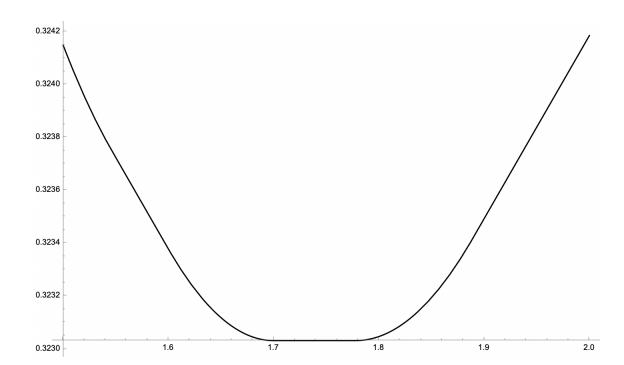
\includegraphics[width=0.58\textwidth]{assets/fig/_page_187_Figure_2.jpeg}
  \caption{\(\xi \in [1.5, 2]\) 范围内 \((2/17^2)(9\xi + I_{\xi}^{17}(\xi))\) 的函数图像片段，显示区间 \(\xi \in [1.7, 1.78]\) 被包含在极小值化范围内.}\label{fig:14.5.1}
\end{figure}

对于分母速率, 先前的计算此时修改为:
\begin{equation}\label{eq:14.5.3}
\tau^{\flat}(\mathbf{b}) = \frac{1 \cdot 0 + (3+5) \cdot 2 + (7+9+11+13+\ldots+33) \cdot 4}{17^2} = \frac{1136}{289},
\end{equation}
并且, 由图~\ref{fig:14.5.1}（其揭示了 \(\xi \in [1.7, 1.78]\) 被包含在极小值化区间内）:

\begin{equation}\label{eq:14.5.4}
\begin{aligned}
\tau^{\sharp}(\mathbf{e}) &= \frac{2}{m^{2}} \min_{\xi \in [0, m]} \left\{ \xi \sum_{i=1}^{m} e_{i} \right. \\
&\quad + \left. \left( \max_{1 \leq i \leq m} e_{i} \right) I_{\xi}^{m}(\xi) \right\} \\
&= \min_{\xi \in [0, 17]} \left\{ (2/17^{2}) \left( 9\xi + I_{\xi}^{17}(\xi) \right) \right\} \\
&= (2/17^{2}) \left( 9 \cdot 7/4 + I_{7/4}^{17}(7/4) \right) = \frac{78419}{242760}.
\end{aligned}
\end{equation}
因此, 我们此时获得了:
\begin{equation}\label{eq:14.5.5}
\tau(\mathbf{b}; \mathbf{e}) = \tau^{\flat}(\mathbf{b}) + \tau^{\sharp}(\mathbf{e}) = \frac{1136}{289} + \frac{78419}{242760} = \frac{1032659}{242760} = 4.2538...,
\end{equation}
这正是在等式 (A.6.2) 中浮现的数值 \(\frac{1032659}{242760}\).

\begin{proof}
我们现在可以通过推导 m < 17 形式的矛盾来再次完成证明. 
以及类似于定理 A 的证明, 这可以通过若干种方式来进行. 
例如：应用定理 7.0.1, 我们获得了公式 (A.6.2) 中计算出的上界 \(m \le 16.2\).
\end{proof}

% 引入第15节内容
\section{补充与进一步问题}\label{sec:15}

我们以对我们方法自然提出的一些进一步开放问题的讨论来结束本论文. 
但首先, 我们更紧密地讨论我们的一些结果与更成熟方法之间的关系.

\subsection{与 Siegel--Bombieri--Chudnovsky 理论的比较}\label{sec:15.1}

定理 C 是一个关于两个参数（受到某些阿基米德约束）的无理性结果. 
在本节中, 我们将定理 C 与此前可通过 G-函数特殊值的通用算术理论获得的结果进行比较. 
我们首先回顾 Siegel 关于 G-函数的定义, 
为此固定一个域嵌入 \(\mathbf{Q} \hookrightarrow \mathbf{C}\):

\begin{definition}[G-function]\label{def:15.1.1}
一个幂级数 \(f(x) = \sum_{n=0}^{\infty} a_n x^n \in \mathbf{Q}[\![x]\!]\) 是一个 G-函数, 
如果它满足以下两个性质:
\begin{itemize}
  \item[(1)] \(f(x)\) 是 holonomic 的：它满足一个系数属于 \(\mathbf{Q}[x]\) 的线性 ODE.
  \item[(2)] \(a_n\) 以及 \(a_n\) 的分母都具有温和的增长速度, 
  具体而言, \(a_0, \dots, a_n\) 的公分母至多关于 n 呈指数增长, 
  并且 \(a_n \in \mathbf{Q} \hookrightarrow \mathbf{C}\) 的最大 Galois 共轭值也至多关于 n 呈指数增长.
\end{itemize}
\end{definition}

由条件 (1) 紧接着有 \(f(x) \in K[\![x]\!]\) 对于某个数域 \(K/\mathbf{Q}\) 成立. 
正如在第 2.2 节中回顾的那样, 
人们期望（参见 \cite{FR17}）对于此类 \(f(x)\), 存在 \(A \in \mathbf{N}_{>0}, b \in \mathbf{Q}_{>0}\) 以及 \(\sigma \in \mathbf{N}\) 使得:
\begin{equation}\label{eq:15.1.2}
a_n A^{n+1} [1, \dots, bn]^{\sigma} \in \mathcal{O}_K \qquad \forall n \in \mathbf{N},
\end{equation}
并且此外, 在 \(f(x)\) 源于几何的附加（猜想上是不必要的）假设下, 
这已经是无条件已知的（参见 \cite[第 V 节附录]{And89}）. 
在任何情况下, 本论文中所有的 holonomic 函数都确实具有被 \eqref{eq:15.1.2} 所包含的分母； 
它们显然是 G-函数.

G-函数算术理论的基本范式由以下定理所刻画:

\begin{theorem}\label{thm:15.1.3}
对于具有有理系数的 G-函数的任意 \(\mathbf{Q}(x)\)-线性无关集合 \(f_1, \dots, f_h \in \mathbf{Q}[\![x]\!]\), 
存在一个可由所有 \(f_i\) 的极小 ODE 有效计算的常数 \(N_0 = N_0(f)\), 
使得集合:
\begin{equation}\label{eq:15.1.4}
\{n \in \mathbf{Z} : f_i(1/n) \text{ 在 } \mathbf{Q} \text{ 上线性相关或包含一发散值}\} \subset [-N_0, N_0].
\end{equation}
\end{theorem}

该结果在 Siegel 1929 年的论文 \cite[第 VII 节]{Zan14} 中得到了展望, 
并由 David 以及 Gregory Chudnovsky \cite{CC85a} 在我们在此陈述的抽象程度上予以了证明, 
这是在 Galo{\v{c}}kin \cite{Gal74} （他不得不假设“因子抵消性质”, 
这反映在可积联络的全局幂零性上； 
Siegel 本人也已经注意到了这一困难）以及 Bombieri \cite{Bom81} （他在与 Galo{\v{c}}kin 最终等价的、但更容易验证的“微分系统是算术 Fuchs 型”的附加假设下证明了一个通用的阿代尔定理） 
的奠基性工作之后完成的. 
Chudnovsky 兄弟的主要成果 \cite[定理 III]{CC85a}（亦见 \cite[定理 VIII.1.5]{DGS94}, \cite[第 VI 节]{And89}, \cite{DV01}） 
正是对于所有至少承认一个 G-级数形式解的不可约 ODE 证明了全局幂零性性质.

\begin{remark}\label{rem:15.1.5}
与第 3.3.3 节的讨论相一致, 关于 Siegel 计划的定量结果当然强于从 Galo{\v{c}}kin, Bombieri 以及 Chudnovsky 兄弟的工作中提取的这一最基本形式. 
关于其他具有密切相关结果的讨论, 参见 Bombieri 在 \cite[第 49 页]{Bom81} 中的主定理\setcounter{footnote}{38}\footnote{注意 Andr{\'e} 的评注 \cite[第 79 页]{And89}：在 Bombieri 主定理的项 $c_{24}$ 中，应在求和式 $\sum_{\zeta \in \operatorname{sing}_0(L)}$ 前增加一个标量系数“2”。}, 
以及 \cite[定理 I 以及 II]{CC85a}, \cite[第 1.2 节主定理]{Deb86}, \cite[第 VII 节]{And89}. 
关于 1997 年之前该学科状况的一幅极佳画卷见于 \cite[第 5 章第 7 节]{PS98}. 
对于更近期的综述, 我们参考 \cite[第 5.6 节]{Riv19}, 
以及 \cite{FR18} 的进一步发展. 
通过根据微分算子使 \(N_0\) 显式化（遵循 \cite{Bom81}）, 
许多标准的放宽形式, 例如允许具有 \(|a/n| < c_1 \exp\left(-c_2\sqrt{\log n \cdot \log\log n}\right)\) 
的显然更一般的代数自变量 \(x = a/n \in \mathbf{Q}\), 
都可以被包含在形式 \eqref{eq:15.1.4} 中. 
但 \eqref{eq:15.1.4} 也是一种直接将有理点与仿射代数曲线以及我们在特定情况下的框架（参见第 15.2 节）联系起来的形式. 
我们将在下一段中评论前一种联系.

虽然 Bombieri 的一般不等式是在任意数域上的阿代尔形式下给出的, 
但定理 15.1.3 中关于有理系数的条件是根本算术性质的, 
并且这对于关于 \(N_0\) 的有效性条款是至关重要的. 
例如, 如果在 \(\{f_1,\ldots,f_h\}:=\{1,f\}\) 的情况下, 
人们希望像注记 8.2.42 中那样处理代数数系数 \(f \in \overline{\mathbb{Q}}[\![x]\!]\)，
基于对称幂的 \cite[第 7 节]{CC85a} 中 Siegel--Shidlovsky 式证明逻辑要求，将假定 \(f(x) \notin \overline{\mathbf{Q}}(x)\)（非有理函数）加强为 \(f(x) \notin \overline{\mathbf{Q}(x)}\)（超越函数）。
事实上，Siegel 关于非有理仿射代数曲线上的整点的有限性定理，至今尚未能给解的高度确定一个有效的上界\footnote{这正是 Hilbert 第十问题在两个变量下的情况的内容。}，但它可以被证明等价于声明 \eqref{eq:15.1.4} 中的 \(f(x) \in \overline{\mathbf{Q}(x)}, \{f_1, \dots, f_h\} = \{1, f\}\) 并且将 \(f \in \mathbf{Q}[\![x]\!]\)（有理系数）的前提放宽为数域系数的情形。 
因此, 对于除 \(\mathbf{Q}\) 或虚二次域之外的数域系数的代数幂级数情况, 
像 \eqref{eq:15.1.4} 这样的声明仍然是一个以及开放\setcounter{footnote}{41}\footnote{同样地，例外的是代数情形 $f_i(x) \in \overline{\mathbf{Q}(x)} \cap \mathbf{Q}[\![x]\!]$，在这种情况下，至少在理论上，有限的计算机搜索就足以在有限的计算时间内解决该问题。}的问题. 
定理 15.1.3 中处理的有理系数情况, 在代数函数 \(f(x) \in \mathbf{Q}(x) \cap \mathbf{Q}[\![x]\!]\) 的情况下, 
被简化为了 Bombieri 对经典 Runge 定理的推广 \cite[定理 9.6.6]{BG06}（亦见 \cite[第 IV 节]{Bom83}）： 
即在 \(\mathbf{Q}\) 上不可约双变量 Diophantine 方程 F(x,y)=0 的最高阶齐次部分在 \(\mathbf{Q}\) 上不与不可约多项式的方幂成比例的前提下, 
在 \((x,y) \in \mathbf{Z} \times \mathbf{Q}\) 上的有效求解. 
（更本质地, 在 Runge 分裂条件下：用于给出 \(\mathbf{C}\)-整点以及 \(\mathbf{Q}\)-有理点概念的“无穷远因子”在 \(\mathbf{Q}\) 上分裂为至少两个不交部分.） \end{remark}

在这些透视下, 我们的定理 C 可以被视为关于特定双变量 G-函数
\begin{equation}\label{eq:15.1.6}
F(x,y) := \log(1-x)\log(1-y)
\end{equation}
在 \((x, y) = (1/n, 1/m)\) 处的特殊值的对应物. 
此类型的至少一些基本结果（参见例如 \cite{Gal74}\cite{Gal75}\cite{Gal96}\cite{Hat98}\cite{Lys18}） 
当然也被包含在单变量定理 15.1.3 中, 
例如人们可以在点 x = 1/n 处评估单变量 G-函数 f(x) = log(1-x) log(1+x). 
在甚至像这般简单的例子上, 
源自通用理论的门槛项 \(N_0\) 是以及巨大的； 
在 \cite{Hat98} 中, 这在当前例子中被估计为处于 \(e^{170}\) 数量级上. 
根据我们的了解, 证明无理性 \(\log(1 - 1/n) \log(1 + 1/n) \notin \mathbf{Q}\) 的记录最低门槛是 Lysov 在 \cite{Lys18} 中通过显式（特殊的！）Hermite--Pad{\'e} 构造获得的 \(n \geq 33\). 
在本节中, 我们研究通用 G-函数方法在我们的定理 C 上的应用范围.

\subsubsection{单变量理论的范围}\label{sec:15.1.7}

为了应用单变量理论, 我们应当将 \(k := m - n\) 视为一参数, 
并考虑在 \(\mathbf{Q}[\![x]\!]\) 中的 G-函数:
\begin{equation}\label{eq:15.1.8}
f(x) := \log(1-x)\log\left(1-\frac{x}{1+kx}\right); \qquad k := m-n \in \mathbf{Z},
\end{equation}
其在 x = 1/n 处的值给出了所需的两个对数的乘积:
\[ f(1/n) = \log(1 - 1/n)\log(1 - 1/m) = F(1/n, 1/m). \]
仅仅为了记号的简单起见，我们在此仅关心乘积 \(\log(1 - 1/n) \log(1 - 1/m)\) 的无理性，
而不关心其与单个因子之间的线性无关性； 
为了展示通用 G-函数特殊值理论的局限性，这当然是足够的。 
因此我们取 \(\{f_1, \dots, f_h\} := \{1, f\}\) 来应用定理 15.1.3。 
那么我们需要将定理 15.1.3 中的 \(N_0 = N_0(k) = N_0(m - n)\) 量化为 k 的函数, 
这本质上是线性 ODE 的高度。

我们断言，对于函数 \(f_k\) 的极小 ODE，根据我们在注记 15.1.5 中列出的、关于通用算术 G-函数理论的任何参考文献中的方法，都有 \(\log N_0(k) \asymp \log |k|\) 成立。\setcounter{footnote}{40}\footnote{我们省略了具体细节，但有进取心的读者可以在该论文发布在 arXiv 上的 LaTeX 源码中找到它们。}
给定这一断言，保证由 \eqref{eq:15.1.4} 给出 \(f(1/n) \notin \mathbf{Q}\) 的条件变为了对于某个绝对常数 \(c \in \mathbf{R}_{>0}\) 有 \(|n| > |k|^c\), 
即条件:
\[ |1 - m/n| < |k/n| < |n|^{1 - 1/c}. \]
这意味着, 定理 C 中可通过通用 G-函数理论推导的情况都在具有如下形式的条件：
\[ 0 < |1 - m/n| \ll |n|^{-\kappa}, \qquad \text{对于某个 } \kappa \in (0, 1) \]
下； 
这一条件是这些通用方法得以应用的充要条件； 
但这一条件明显强于我们的 \(0 < |1 - m/n| < 10^{-6}\).

\subsubsection{多变量 G-函数理论}\label{sec:15.1.9}

多变量 G-函数的算术理论仍然处于其起步阶段； 
我们参考 \cite{AB97} 以获取几何基础, 
并参考 \cite{Nag97}（针对二维）以及 \cite{DV01}（针对任意维数）以获取 Chudnovsky 兄弟基本定理的推广. 
极有可能的是, 由 Bombieri 在 \cite{Bom81} 中执行的、自动机形式方案的二维版本, 
可以与关于在特殊点处的 Diophantine 辅助构造的、标准的非消逝方法相组合, 
以便给出双变量 G-函数 \(f(x,y) \in \mathbf{Q}[\![x,y]\!] \setminus \mathbf{Q}(x,y)\) 在形如 x=1/n, y=1/m 
（伴随着满足 \(\log |n| \gg_f 1\) 以及 \(\log |m|/\log |n| \gg_f 1\) 的 \(n,m \in \mathbf{Z} \setminus \{0\}\)） 
的自变量处特殊化值的无理性结果 \(f(1/n,1/m) \notin \mathbf{Q}\)； 
根据我们的了解, 此类计划在文献中尚未被研究过. 
我们为 \eqref{eq:15.1.6} 从 Ap{\'e}ry 极限方法获得的范围 \(|1-m/n| < 10^{-6}\) 与此是完全正交的！

\subsubsection{来自 Hermite--Pad{\'e} 构造的途径}\label{sec:15.1.10}

正如我们在第 3.3.7 以及 3.3.13 节中解释的, 
我们在第 14 节中对定理 C 的证明可以概念性地与对数函数的 Hermite--Pad{\'e} 逼近以及第 14.1 节中 Hadamard 乘积构造的使用联系起来. 
虽然三个或更多对数的乘积由于数值关系 \(e^3 > 16\) 似乎无法通过我们的方法触及, 
但尝试起步于在 \cite{RT86} 以及 \cite{DHKK22} 中显式研究的、关于若干对数的联立 Hermite--Pad{\'e} 逼近理论, 
来证明多于一对的两个对数乘积的线性无关性, 将会是非常有价值的.

一种更一般的方案, 正如我们在第 3.3.3 以及 3.3.7 节中在最基本的例子上指出的那样, 
可以通过形成由对一基本函数评估一正规形式的 Hermite--Pad{\'e} 逼近序列而获得的特殊线性形式的生成函数来予以寻求. 
Beukers \cite{Beu81}\cite{Beu84} （利用多重对数）以及 Pr{\'e}vost \cite{Pre96} （具有 \(\zeta(3, 1+1/y)\) 作为要在形如 y=1/n 处评估的基本函数）, 
各自都能够在这样的方案内解释 Ap{\'e}ry 序列. 
前一种类型被 Fischler 以及 Rivoal \cite{FR03} 极大地推广了. 
在我们在第 11 节中利用的、在 \(\zeta(2)\) 以及 \(L(2,\chi_{-3})\) 上的联立线性形式的语境下, 
寻找类似的 Hermite--Pad{\'e} 逼近解释也将会是非常有趣的. 
然而, 我们评述：即使开始于 Hermite--Pad{\'e} 逼近的函数是代数的, 
此类生成级数程序也远非总是产生 G-函数 \cite{BC97b}； 
对于 Pr{\'e}vost 类型, 与 zeta 值相关的一些反例见于 \cite[第 8 节]{PR21}.

我们以及在此处省略（部分是由于空间原因）的另外两个课题是： 
向关于两个对数的非有理代数自变量的应用, 
以及 p-进对数. 
省略后一应用的另一个原因是在本论文中, 
我们在涉及超收敛性时强调了阿基米德地方作为特殊地方的地位. 
在 \cite{CDT24} 中, 我们计划在全局域上的更一般的 Arakelov 阿代尔形式下写出我们的 holonomicity 边界.

最后, 更广泛地讨论任何方法下的 holonomic 显式构造, 
我们评述：在文献中许多更复杂的构造中——例如在 Zudilin 关于 \(\zeta(2)\) 以及 \(\zeta(3)\) 联立逼近的工作 \cite{Zud14} 中, 
以及在 Brown 以及 Zudilin 关于 \(\zeta(5)\) 的工作 \cite{BZ22} 中——向尚未达到的无理性目标的进展是通过设置一个复杂的参数集来极大化卓越指数 \(\limsup \left\{-\frac{\log |\eta - p/q|}{\log q}\right\}\) 
来衡量的. 
后者远非能忠实地衡量作为在我们有理 holonomy 边界框架内应用潜在性的卓越程度.

\subsection{整 holonomic 模}\label{sec:15.2}

尽管定理 15.1.3 中的 \(N_0\) 是有效的, 
但精确（在原理上）确定 \eqref{eq:15.1.4} 中的左手边集合仍然是一个以及开放\footnote{再一次，例外是一个$f(x)\in \overline{\mathbf{Q}(x)} \Cap \mathbf{Q}[x]\ $，并且是理论上可以通过在有限时间通过计算机穷举得到}的问题. 
此外, 正如我们在像 \cite{Hat98} 这样简单的案例中看到的那样, 
在一般性质 \eqref{eq:15.1.4} 中关于 \(N_0\) 的边界在实践中是非常巨大的. 
我们在第 2.7 以及 2.8 节中关于 \(\mathbf{Q}\left[x, \frac{1}{1-x}\right]\)-整性精细化（特别是参见注记 2.7.6 以及 2.8.2）的发现, 
似乎指向了一种完全不同于那些其 holonomicity 被 Andr{\'e} 算术准则（推论 2.6.1）所识别的、关于 \eqref{eq:15.1.4} 情况的方法. 
我们出于在相似的其他潜在线性无关性设定（其中许多仍是未证明的猜想）中应用的目的而希望逆转注记 2.7.6 中证明逻辑的启示, 
源于 B{\'e}zivin 以及 Robba \cite{BR89} 的想法, 
他们利用这些想法作为 Bertrandias 算术有理性准则 \cite[定理 5.4.6]{Ami75} 的应用重刷了 Hermite--Lindemann--Weierstrass 定理（见 \cite{BBR90} 以获取该证明的历史解剖）； 
以及归根结底, 源于 Andr{\'e} \cite{And00a}\cite{And00b} 以及 Beukers \cite{Beu06} 对这些想法的精细化, 
他们利用 Chudnovsky 兄弟定理以及在 E- 以及 G-函数之间的 Fourier--Laplace 对偶性, 
重刷（以及进一步精细化）了关于 E-函数特殊值的定性 Siegel--Shidlovsky 定理.

设 \(\partial := x \cdot (d/dx)\) 是乘法不变导数. 
考虑（为了在此处的简单起见）一个满足 \(\varphi(0) = 0\) 的 {\'e}tale\footnote{换句话说：导数 $\varphi'$ 在 $\mathbf{D}$ 上处处非零。}全纯映射 \(\varphi : \mathbf{D} \to \mathbf{C}\), 
以及一个向量 \(\mathbf{b} := (b_1, \dots, b_r) \in [0, \infty)^r\) 
满足 \(|\varphi'(0)| > e^{b_1 + \dots + b_r}\). 
考虑由满足如下形状的形式幂级数组成的集合 \(\mathcal{D}\):
\begin{equation}\label{eq:15.2.1}
f(x) = \sum_{n=0}^{\infty} a_n \frac{x^n}{\prod_{i=1}^r [1,\dots,b_i \cdot n]}, \quad a_n \in \mathbf{Z} \quad \forall n \in \mathbf{N}
\end{equation}
使得 \(\varphi^* f \in \mathcal{O}(\mathbf{D})\) 是圆盘上的全纯函数。这是一个在非交换环 \(\mathbf{Z}[x,\partial]\) 上的模：
求导作用于单项式为 \(\partial(x^n) = nx^n\)，这保持了 \eqref{eq:15.2.1} 中的整性类型，而复合函数求导法则结合 \(\varphi\) 的 étaleness 表明，如果 \(f(\varphi(z))\) 是全纯的，那么下式也是全纯的：
\[ \frac{\varphi(z)}{\varphi'(z)} \left( f(\varphi(z)) \right)' = \varphi(z) f'(\varphi(z)) = (\partial f)(\varphi(z)). \]
根据构造，\(\mathbf{Z}[x,\partial]\)-模 \(\mathcal{D}\) 嵌入为环 \(\mathbf{Q}[\![x]\!]\) 的子模。在这个环境环中，\(\mathcal{D}\) 包含了由满足 \(\varphi^*\alpha \in \mathcal{O}(\mathbf{D})\) 的 \(\alpha \in \mathbf{Z}[\![x]\!]\) 组成的子环。为了与 \cite{BC22} 和我们的注记 7.3.2 保持一致，我们将该环记为 \(\mathcal{O}(\widetilde{\mathcal{V}})\)（在此我们将其视作形式解析\footnote{如果 $\varphi$ 可以延拓为闭圆盘 $\overline{\mathbf{D}}$ 的某个开邻域上的全纯函数，这与 \cite{BC22} 中的约定相符。为了应用有限性定理 \cite[定理 9.1.1]{BC22}，通过考虑 $\widetilde{\varphi}(z) := \varphi((1-\varepsilon)z)$（其中 $\varepsilon > 0$ 足够小以至于仍然满足 $|\widetilde{\varphi}'(0)| > e^{b_1 + \cdots + b_r} > 1$），这并不是一个限制。}算术表面 \(\widetilde{\mathcal{V}} := \widetilde{\mathcal{V}}(\varphi)\) 上的正则函数环）。那么 \(\mathcal{D}\) 是一个在环 \(\mathcal{O}(\widetilde{\mathcal{V}})\) 上的模。

由 Andr{\'e} 准则（推论 2.6.1），分数域 \(\operatorname{Frac}(\mathcal{O}(\widetilde{\mathcal{V}}))\) 是 \(\mathbf{Q}(x)\) 的有限域扩张，并且 \(\mathcal{D} \otimes_{\mathcal{O}(\widetilde{\mathcal{V}})} \operatorname{Frac}(\mathcal{O}(\widetilde{\mathcal{V}}))\) 是该域上的有限维向量空间。由于此外 \(\mathcal{D}\) 在求导 \(\partial\) 的作用下是保持不变的，因此存在一个有限且 \(\operatorname{Gal}(\overline{\mathbf{Q}}/\mathbf{Q})\)-稳定的复代数点集 \(\Sigma \subset \overline{\mathbf{Q}} \hookrightarrow \mathbf{C}\)，使得 \(\mathcal{D} \otimes_{\mathcal{O}(\widetilde{\mathcal{V}})} \operatorname{Frac}(\mathcal{O}(\widetilde{\mathcal{V}}))\) 的所有元素（从而尤其是 \(\operatorname{Frac}(\mathcal{O}(\widetilde{\mathcal{V}}))\) 的所有元素）都可以解析延拓为 \(\mathbf{C} \setminus \Sigma\) 中沿着所有路径的亚纯函数。

然而，Bost 和 Charles 证明了一个更深层次的有限性定理 \cite[定理 9.1.1]{BC22}：环 \(\mathcal{O}(\widetilde{\mathcal{V}})\) 是一个有限生成的 \(\mathbf{Z}\)-代数。此外，他们的证明在原理上给出了一种有效算法，用于列出该 \(\mathbf{Z}\)-代数的有限生成元集。另一方面，正如在 \(\mathbf{b} = (1)\) 且 \(\varphi(z) = 4z/(1+z)^2\) 的例子中注记 2.7.5 所展示的那样（此时 \(\mathcal{O}(\mathcal{V}) = \mathbf{Z}[x,1/(1-x)]\)），\(\mathcal{O}(\widetilde{\mathcal{V}})\)-模 \(\mathcal{D}\) 一般是无限的。因此，我们将其与 \(\mathbf{Q}\) 作张量积并考虑 \(\mathcal{D}_{\mathbf{Q}} := \mathcal{D} \otimes_{\mathbf{Z}} \mathbf{Q}\)，它是环 \(\mathcal{O}(\mathcal{V}_{\mathbf{Q}}) := \mathcal{O}(\mathcal{V}) \otimes_{\mathbf{Z}} \mathbf{Q}\) 上的一个无扭模。后一个环\footnote{这是我们在此处的特有记号，并不出现在 \cite{Bos20} 或 \cite{BC22} 中。}是一个有限生成的 \(\mathbf{Q}\)-代数，但同时，由于它的 Krull 维数为 1 且在其分数域中是整闭的，它还具有作为一个 Dedekind 整环的额外便利。在 Dedekind 整环上的一个模是有限且无扭的，当且仅当它是有限秩局部自由的，当且仅当它是投射且一般有限的（其中后者意味着诱导的分数域上向量空间具有有限维数）。定理 2.7.2 的内容是，在之前 \(\mathbf{b} = (1)\) 和 \(\varphi(z) = 4z/(1+z)^2\) 的例子中，\(\mathcal{O}(\widetilde{\mathcal{V}}_{\mathbf{Q}})\)-模 \(\mathcal{D}_{\mathbf{Q}}\) 是一个以 \(\{1, \log(1-x)\}\) 为基的 2 秩自由模。然而，注记 2.7.4 的内容是，在稍加修改的例子 \(\mathbf{b} = (1 + 1/100)\) 和 \(\varphi(z) = 4z/(1+z)^2\) 中（仍然满足 \(\mathcal{O}(\widetilde{\mathcal{V}}) = \mathbf{Z}[x, 1/(1-x)]\) 和 \(\mathcal{O}(\widetilde{\mathcal{V}}_{\mathbf{Q}}) = \mathbf{Q}[x, 1/(1-x)]\)），\(\mathcal{O}(\widetilde{\mathcal{V}}_{\mathbf{Q}})\)-模 \(\mathcal{D}_{\mathbf{Q}}\) 是无限生成的。

\begin{question}\label{qu:15.2.2}
是否可以有效构造一个 \(h \in \mathcal{O}(\widetilde{\mathcal{V}}) \setminus \{0\}\)，使得：
\begin{itemize}
  \item[(\(*\))] 模 \(\mathcal{D}_{\mathbf{Q}}[1/h]\) 在环 \(\mathcal{O}(\widetilde{\mathcal{V}}_{\mathbf{Q}})[1/h]\) 上是局部自由的？
\end{itemize}
是否存在一些自然的可验证条件，使得上述结论即使在 \(h = x\) 时也成立？
\end{question}

如上所述，环 \(\mathcal{O}(\widetilde{\mathcal{V}}_{\mathbf{Q}})\) 及其局部化是 Dedekind 整环，因此，由于 \(\mathcal{O}(\widetilde{\mathcal{V}}_{\mathbf{Q}})[1/h]\)-模 \(\mathcal{D}_{\mathbf{Q}}[1/h]\) 是无扭且一般有限的，\((\star)\) 中的局部自由性等价于该模是有限的，也等价于该模是投射的。我们将会看到，为什么坚持有效性对于从 holonomic 模 \(\mathcal{D}\) 导出某些函数在 \(x=1/n\) 处的特殊值的无理性证明至关重要。这种联系的原因与 Andr{\'e}--Beukers 关于 Siegel--Shidlovsky 定令的（定性）精细化 \cite{And00a, And00b, Beu06} 最终源自一个在形式上类似于 \((\star)\) 的交换代数命题完全相同：

\begin{fact}\label{fact:15.2.3}
具有有理系数的 E-函数环 \(\mathbf{E} \subset \mathbf{Q}[\![x]\!]\) 在 Laurent 多项式环 \(\mathbf{Q}[x,x^{-1}]\) 上生成了一个无限自由的 \(\mathbf{Q}[x,x^{-1}]\)-模 \(\mathbf{E}[1/x] = \mathbf{E} \otimes_{\mathbf{Q}[x]} \mathbf{Q}[x,x^{-1}]\)。
\end{fact}

关于此声明参见 \cite[定理 1.5]{Beu06}\footnote{Kaplansky 的一个定理（参见 \cite[第 4.1.2 节]{Bos20}）表明，在一个 Dedekind 整环上，任何投射且可数生成、但非有限生成的模都是自由模。因此，\(\mathbf{E}[1/x]\) 的 \(\mathbf{Q}[x,x^{-1}]\)-自由性简化为了其所有有限生成 \(\mathbf{Q}[x,x^{-1}]\)-子模的自由性，即 \cite[定理 1.5]{Beu06}。}，关于其机制参见 \cite[推论 2.2 的证明]{Beu06}。这里对 \(x\) 求逆也是必需的，正如我们在例子 \(\mathbf{b} = (1+1/100)\) 和 \(\varphi(z) = 4z/(1+z)^2\) 下的 \((\star)\) 中看到的那样。在 E-函数的背景下，以
\[ \left\{ (d/dx)^j \left\{ \frac{e^x - 1}{x} \right\} : j \in \mathbf{N} \right\} \]
为例。该集合生成了一个无限的 \(\mathbf{Q}[x]\)-模，其局部化为一个以 \(\{1,e^x\}\) 为基的 2 秩自由 \(\mathbf{Q}[x,x^{-1}]\)-模。在 Andr{\'e}--Beukers 理论中 \(x=0\) 的特殊角色，反映了像 \(f(x)=e^x\) 这样的超越 E-函数的存在，其极小 ODE 并不以 0 为奇点，但其特殊值 \(f(0)=1\in\mathbf{Q}\) 却是有理数。

如果问题 15.2.2 具有肯定的回答，那么存在一个类似于 \cite{BR89, And00b, Beu06} 的形式机制来导出线性无关性证明。假设 \(h \in \mathcal{O}(\widetilde{\mathcal{V}}) \setminus \{0\}\) 使得局部化 \(\mathcal{O}(\widetilde{\mathcal{V}}_{\mathbf{Q}})[1/h]\)-模 \(\mathcal{D}_{\mathbf{Q}}[1/h]\) 是局部自由的。现在另外假设，如第 2.9 节中那样，存在一个收缩开邻域 \(0 \in \Omega \subset \mathbf{D}\)，\(\varphi\) 在该邻域上限制为一个单值映射，并且满足 \(\varphi^{-1}(\Sigma) \subset \Omega\)。考虑 \(f(x) \in \mathcal{D}_{\mathbf{Q}}\) 和一个包含 \(\Sigma\) 的、有限的、\(\operatorname{Gal}(\overline{\mathbf{Q}}/\mathbf{Q})\)-稳定的复代数点集 \(S_f \subset \overline{\mathbf{Q}} \hookrightarrow \mathbf{C}\)，使得 \(f(x)\) 沿着 \(\mathbf{C} \setminus S_f\) 中的所有路径全纯延拓。进一步假设这些不同的解析延拓最终在点 \(x = 1/n\) 处至少取得两个不同的值。

现在假设 \(n \in \mathbf{Z} \setminus \{0\}\) 满足以下限制：
\begin{enumerate}
  \item[(1)] \(\varphi^{-1}(1/n) \subset \Omega\)；
  \item[(2)] \(1/n \notin S_f\)；
  \item[(3)] 元素 \(h\) 在 \(\mathbb{C}^1 \setminus \Sigma\) 中的所有解析延拓在点 \(1/n\) 处都取非零值。
\end{enumerate}
那么特殊\footnote{这指的是在 \(x = 1/n\) 处评估的 \(\mathbf{Q}[\![x]\!]\) 级数；因此出现了“要么是无理数，要么是发散值”的通常二分法。然而，我们在此处可以说出更精确的结论：值 \(f(1/n) \in \mathbf{C}\) 是无理数，该值通过从 \(x = 0\) 开始、保持在单值叶 \(\Omega \supset \{0, 1/n\}\) 内的解析延拓而定义良好。最近，Fischler 和 Rivoal \cite{FR21} 成功地将某些 G-函数纳入了超出收敛圆盘的特殊值的 Ball--Rivoal 框架中。}值 \(f(1/n)\) 满足类似于 \eqref{eq:15.1.4} 的无理性性质：要么 \(f(1/n) \notin \mathbf{Q}\)，要么 \(f(1/n)\) 是发散的。

其论点在形式上与 \cite{Beu06} 相同。存在一个非零多项式 \(Q_f \in \mathbf{Z}[x] \setminus \{0\}\) 使得 \(\{Q_f = 0\} = S_f\) 并且 \(Q_f(x)f(x)\) 沿着 \(\mathbf{C} \setminus \Sigma\) 中的所有路径全纯延拓。如果 \(f(1/n) = p/q\) 是有理数，那么第 2.9 节中我们设定中的局部单值性性质 (1) 将适用于函数
\[ \widetilde{f}(x) := Q_f(x) \frac{f(x) - f(1/n)}{1 - nx} \in \mathbf{Q}[\![x]\!], \]
（其中 \(\Sigma^1 := \{s \in \Sigma : \varphi^{-1}(s) = \emptyset\}\)，而 \(\Sigma^0 := \{1/n\} \cup (\Sigma \setminus \Sigma^1)\)，并且命题 2.9.3 中的 \(\Sigma\) 扩充为 \(\Sigma \cup \{1/n\}\)），从而导出
\begin{equation}\label{eq:15.2.4}
\partial^{j}\left\{\widetilde{f}(x)\right\} \in \mathcal{D}_{\mathbf{Q}}, \quad \text{对于所有 } j \in \mathbf{N} \text{ 成立。}
\end{equation}
假设 \((\star)\)、(2) 和 (3) 意味着函数 \eqref{eq:15.2.4} 生成了一个有限的 \(\mathbf{C}(x)\)-模，同时也生成了一个有限的 \(\mathbf{C}[\![\frac{1}{1-nx}]\!]\)-模。因此，\(\mathcal{L}(\widetilde{f})=0\) 对于某个在点 \(x=1/n\) 处非奇异的、 \(\mathbf{C}(x)\) 上的非零线性微分算子 \(\mathcal{L}\) 成立。但这与我们的条件冲突：\(\widetilde{f}\) 具有某个解析延拓 \(\widetilde{F}\)（它必然也是 ODE \(\mathcal{L}(\widetilde{F})=0\) 的解），使得 \(x=1/n\) 是 \(\widetilde{F}(x)\) 的一个亚纯极点。

这使得为问题 15.2.2 中的有限性性质 \((\star)\) 构造一个元素 \(h \in \mathcal{O}(\widetilde{\mathcal{V}}) \setminus \{0\}\) 具有极高的价值。作为一个简单的例子，如果 \(h=1\) 或仅仅 \(h=x\)（类似于 Andr{\'e}--Beukers 的事实 15.2.3 以及前文的讨论）对于基本注记 2.11.1 的二价映射 \(\varphi(z) = 8(z+z^3)/(1+z)^4\) 和 \([1,\ldots,n]^2\) 分母类型（\(\mathbf{b}=(1,1)\)）是允许的，那么仅凭这一点就足够了——无需在那种背景下证明可能更为困难的完整猜想 2.8.1——将注记 2.8.2 嵌入上述讨论中，并一举得出其余值 \(n \in \{-4, -3, -2, 2, 3, 4, 5\}\) 的无理性 \(\mathrm{Li}_2(1/n) \notin \mathbf{Q}\)。事实上，在这个例子中，一个简单的计算（例如参见 \cite{Rob68}）给出了 \(\mathcal{O}(\widetilde{\mathcal{V}}) = \mathbf{Z}[x, 1/(1-x)]\)，其中 \(\Sigma = \{0, 1, \infty\}\)，而对于 \(\Omega\)，我们可以取 \((-1, 1)\) 在 \(\mathbf{D}\) 中的任何足够小的开邻域，使得满足 \(\varphi^{-1}(\varphi(\Omega)) = \Omega\)。 \(\vartriangle\)

\subsection{线性无关性的定量特征}\label{sec:15.3}

正如在超越数论中通常\setcounter{footnote}{46}\footnote{除了 Andr{\'e} 以及著名的 transcendence sans transcendence \cite{And00a}\cite{And00b} 之外, 
该工作应用了 G-函数的算术理论来重新获得关于 E-函数的 Siegel--Shidlovsky 定理.}所作的那样, 
我们本文中的线性无关性证明在原理上可以被推向关于相关周期线性形式的定量下界估计. 
然而, 在当前情况下, 这一过渡并不是平凡的, 
并需要大量的额外工作, 我们决定不在本文中涉及这些内容. 
第 3.3.3 节的讨论指出了做出此类过渡的第一步方法论线索. 
我们计划在未来的工作中转向它.

\subsection{结构环}\label{sec:15.4}

阐明如定理 2.7.2（关于 \(\log x\)）、定理 2.8.4（关于 \(\log^2 x\)）等算术代数化定理的范围, 
以及在 \(\mathbf{P}^1 \setminus \{0,1,\infty\}\) 上关于 \([1, \ldots, n]^2\) 
层 G-函数的更精确猜想 2.8.1 的范围, 
将会是非常有趣的. 
例如, 人们可以问：第 10.3 节的多重 polylogarithm 环有多少可以被算术代数化术语所捕捉. 
以下问题超出了我们方法论的范畴:

\begin{question}\label{qu:15.4.1}
考虑由满足如下形式的 G-函数 \(f(x)\) 
在 \(\mathbf{P}^1 \setminus \{0, 1, \infty\}\) 上几何来源的、
由 \(\mathbf{Q}(x)\)-向量空间 \(\mathcal{H}\):
\begin{equation}\label{eq:15.4.2}
f(x) = \sum_{n=0}^{\infty} a_n \frac{x^n}{[1, \dots, n]^3} \in \mathbf{Q}[\![x]\!], \qquad a_n \in \mathbf{Z} \quad \forall n \in \mathbf{N}
\end{equation}
所生成的空间. \(\mathcal{H}\) 是否为有限维的？
\end{question}

满足 \(\varphi(0)=0\) 以及 \(\varphi^{-1}(0)=\{0\}\) 的万有映射 \(\varphi: \mathbf{D} \to \mathbf{C} \setminus \{1\}\) 是 \(\lambda\). 
由于有 \(16 < e^\pi = e^3\), 
我们的方法对问题 15.4.1 没有任何直接可以说的内容； 
我们甚至无法猜测答案会是什么. 
（相比之下, 对于分母类型——例如——\([1, \ldots, n]^2[1, \dots, n/2]\) 
或 \(\prod_{k=1}^8 [1, \dots, n/k]\), 
推论 2.6.1 证明了在 \(\mathbf{P}^1 \setminus \{0, 1, \infty\}\) 上的对应 G-函数形成了一个有限维空间, 
尽管要确定这些空间即使在猜想上可能也是相当困难的.）

\text{我们强调：即使当 \(\tau = 0\) 时, 该问题也并不见得更简单；} 
人们可以问：对于哪些 \(\alpha \in \mathbf{Q}\), 
在 \(\mathbf{P}^1 \setminus \{0, \alpha, \infty\}\) 
上由满足 \(\mathbf{Z}[\![x]\!]\) 
的有理系数代数幂级数 \(f(x)\) 所生成的 \(\mathbf{Q}(x)\)-向量空间 is 无限维的. 
该空间当 \(\alpha > 1/16\) 时是有限维的, 
以及当 \(\alpha = 1/16\) 时是无限维的, 
在后者情况下, 人们可以通过在同余子群上写出具有整系数的模函数并用 \(x = \lambda/16\) 
作为自变量来构造这些函数. 
\cite{CDT21} 的主要成果是证明了所有此类 \(f(x)\) 都是以此方式出现的. 
但一旦有 \(\alpha < 1/16\), 我们就没有任何方法来理解这一问题, 
甚至无法确定在 \(\mathcal{H}\) 中是否存在一个单单的非有理函数. 
然而, 人们可以借助 \(\alpha = 1/16\) 这一例子来展示：对于某些满足 \(\tau > 0\) 
的模板, G-函数的空间确实是无限维的.

\begin{proposition}\label{prop:15.4.3}
令 \(\mathcal{H}\) 表示在 \(\mathbf{P}^1 \setminus \{0,1,\infty\}\) 
上由来自几何来源的、满足如下形式的 G-函数 \(f(x)\) 
所生成的 \(\mathbf{Q}(x)\)-向量空间:
\begin{equation}\label{eq:15.4.4}
f(x) = \sum_{n=0}^{\infty} a_n \frac{x^n}{[1, \dots, 2n]^2} \in \mathbf{Q}[\![x]\!], \qquad a_n \in \mathbf{Z} \quad \forall n \in \mathbf{N}.
\end{equation}
那么 \(\mathcal{H}\) 是无限维的.
\end{proposition}

\begin{proof}
设 \(g(q) \in \mathbf{Z}[\![q]\!]\) 是在 \(X_0(N)\) 上偏离尖点全纯的模函数. 
那么, 将 \(g(q)\) 作为 \(x = \lambda/16\) 的函数写出来, 
我们发现 \(g(x) \in \mathbf{Z}[\![x]\!]\) 是在 \(\mathbf{P}^1 \setminus \{0, 1/16, \infty\}\) 
上的代数函数, 
并且（通过取越来越大的 N）此类 \(g(x)\) 的空间在 \(\mathbf{Q}(x)\) 
上是无限维的. 
现在设:
\[ h(x) = {}_{3}F_{2}\left[\begin{smallmatrix} 1/2, & 1/2, & 1 \\ & 3/2, & 3/2 \end{smallmatrix} ; \frac{x}{16}\right] = \sum \frac{x^{n}}{\binom{2n}{n}^{2}}. \]
函数 \(h(x)\) 具有分母类型 \(\tau = [1, 2, 3, ..., 2n]^2\) 
并且是在 \(\mathbf{P}^1 \setminus \{0, 16, \infty\}\) 上的几何来源 G-函数. 
现在, Hadamard 乘积:
\[ f(x) = g(x) \star h(x) \]
位于 \(\mathcal{H}\) 中, 并在 \(\mathbf{Q}(x)\) 
上生成了一个无限维空间.
\end{proof}

注意该情况下的数值巧合对应于 \(e^4 > 16\).

\subsection{算法问题}\label{sec:15.5}

给定一个几何来源的 ODE, 人们在一般情况下总是可以给出分母类型的一个上界. 
然而, 确定分母的精确增长速度在一般情况下似乎是困难的. 
两个启发性的例子可以给出如下. 
在 \cite{Coo12} 中, 考虑了以下例子. 
设
\[ x = q \prod_{n=1}^{\infty} \left( \frac{(1-q^{7n})}{(1-q^n)} \right)^4, \]
它是 \(X_0(7)\) 的一个 hauptmodul. 
存在一个对应的、关于 \(X_0(7)^+\) 的统一化参数如下:
\[ y = \frac{x}{1 + 13x + 49x^2}. \]
如果我们现在取权重 2 的 Eisenstein 级数:
\[
\begin{aligned}
E &= \frac{7E_2(\tau) - E_2(7\tau)}{1 - 7} \\
&= 1 + 4q + 12q^2 + 16q^3 + 28q^4 + \dots
\end{aligned}
\]
并且随后将其写为 y 的函数, 
我们获得了一个在 \(\mathbf{P}^1 \setminus \{0, 1/27, -1, \infty\}\) 
上没有奇点的一阶三线性 ODE, 该 ODE 显式地由 \(\mathcal{L}H_A(x) = 0\) 
以及下式给出:
\[ \mathcal{L} = x^{2}(1+x)(-1+27x)\frac{d^{3}}{dx^{3}} + 3x(-1+39x+54x^{2})\frac{d^{2}}{dx^{2}} + (-1+86x+186x^{2})\frac{d}{dx} + 4(1+6x). \]

如果人们考虑非齐次版本 \(\mathcal{L}H(x) = -1\), 
那么存在一个在尖点 1/27 之外超收敛的全纯解 H(x). 
该解是模来源 of, 
也就是存在一个权重 4 of 模形式, 
其三阶（Eichler）积分写为关于参数 q of 函数形式时给出了 \(H(x)/H_A(x)\). 
该例子中不寻常的一点是：权重 4 of 形式是亚纯而非全纯的； 
它对于在 \(S_6(\Gamma_0(7), \mathbf{Q})\) 中的唯一 Hecke 特征形式 h 具有形式 h/E, 
以及因此 h/E 在偏离尖点的地方具有极点. 
但也许更令人惊讶的是, 形式 h/E 在 \cite{BZ19} 的意义下是“磁性”的（magnetic）； 
也就是说, 如果 \(h/E = \sum a_n q^n\), 
那么对于所有 n 均有 \(n|a_n\). 
作为这一结果的一个结果, 
全纯解 H(x)——从所有的外观来看（以及鉴于构建 H(x) 所需的三次积分, 人们本应该期望其具有分母类型 \(\tau = [1, 2, \dots, n]^3\)）——其实际上具有分母类型 \(\tau = [1, 2, \dots, n]^2\). 
这从 ODE 来看是完全不明显的, 
并且目前不清楚是否存在一个先验地计算该结论的算法. 
作为一个奇特的、以及在我们的有理 holonomy 边界框架内应用潜在性的结果, 它也意味着：对应于 Cooper 序列的 Ap{\'e}ry 极限的无理性是可以通过我们的方法触及的； 
然而, 由于对应的常数似乎是 \(\pi^2/42\), 我们并未转向去研究它！

突出计算分母类型困难的第二个例子如下. 
伴随 Ramanujan 的模形式 \(\Delta = \sum \tau(n)q^n\), 
人们可以写下一个对应于 Eichler 积分 \(\sum \tau(n)n^{-11}q^n\) 的非齐次解. 
人们期望所产生函数的分母类型将为 \([1,2,\ldots,n]^{11}\). 
然而, 如果人们可以证明它\textit{不具有} \(A^n[1,2,\ldots,n]^{10}\) 的形式, 
那么人们就将已经证明了对于 \(\Delta\) 存在着无限个普通素数（ordinary primes）, 
这是一个以及著名的开放问题.

\subsection{Gelfond--Schnirelman 主题}\label{sec:15.6}

我们回顾定理 2.7.10 以及基础特例的命名, 
我们基于该特例对对数函数进行了算术代数化： 
狭缝平面区域 \(\Omega := \mathbb{C} \setminus [1, \infty)\) 
具有满足 \(\varphi(z) = 4z/(1+z)^2\) 的 Riemann 映射共形半径 \(\rho(\Omega, 0) = 4\), 
并且它承认超越解析函数 \(\log(1-x) = -\sum_{n=1}^{\infty} x^n/n\), 
其分母类型可以用具有 r=1 以及 \(b_1 = 1\) 的形式 \eqref{eq:2.7.8} 来表达. 
我们在该例中对于 \eqref{eq:2.7.9} 的右手边有 \((2/3) \log 4 = 0.924196 \dots\).

这引出了另一个被 \cite[§ II]{Chu83a} 以及 \cite[第 493--494 页]{FW08} 所考虑的通俗主题, 
这大概是由于其与我们描述的 G-函数算术理论创造者们的方法论相关性. 
这是 Gelfond 以及 Schnirelman 在 1936 年观察到的旧想法, 
他们指出：仅仅通过对在 \([1,\ldots,2n+1]\int_0^1 (t-t^2)^n dt \in \mathbf{N}_{>0}\) 
内逐点 \(\leq 4^{-n}\) 的被积函数进行评述, 
就可以一举推导出素数计数下界 \(\pi(X) > (\log 2)X/\log X\) 对所有 \(X \gg 1\) 成立. 
利用 \(\log(1-x)\) 的 functional bad approximability 性质（第 3.3.7 节中 Hermite--Pad{\'e} 表的正则性）, 
定理 2.7.2 证明中素数定理的使用可以被逆转, 
以便设计出一个关于集成素数计数函数估计的有理 Gelfond--Schnirelman 风格的初等证明： 
对所有足够大的 X, 均有 \(\int_1^X \psi(t) dt > (4/3) \log 2 \cdot X^2/2\). 
这里的系数比 Chebyshev 的 \(\log \left(2^{1/2}3^{1/3}5^{1/5}30^{-1/30}\right) = 0.921292\ldots\) 
稍微好一些, 并且现在的关键在于该证明其实并不是新的： 
它是与 Bombieri、Nair 以及 Chudnovsky 
通过在多元方法中使用判别式\setcounter{footnote}{48}\footnote{在 Bombieri 的情况下，这一探究导致了 Selberg 积分的重新发现，并且以此为真正的数学成果，带来了 Dyson--Mehta 猜想的历史性证明以及 Macdonald 猜想的部分情形。这一故事详述于 \cite[第 1.2、1.3 节]{FW08}。}多项式而获得的开端估计完全同构的论证； 
参见 \cite[第 94 页]{Chu83a}, 
并注意来自 \cite[定理 1 证明]{Nai82} 的 Cauchy 行列式正是应用于我们首节第 1.2.5 节的函数 \(\log(1-x)\) 的 Hankel 行列式. 
由于素数定理的逻辑可以在我们的每一个算术 holonomy 边界中被逆转, 
人们不能不对我们 holonomy 边界的“渐近近失”（asymptotic near-misses）中的分母算术感到好奇.

\subsection{历史注记以及致谢}\label{sec:15.7}

我们最初在 2020 年构想了我们的新无理性方法, 
起步于对 \(\zeta(5)\) 的 2-进化身无理性的一个容易证明（我们最终在伴随论文 \cite{CDT24} 中予以了阐明）, 
以及甚至在当年我们就在 \cite{Zag09} 的帮助下意识到：该方法在原理上可以应用于 \(L(2,\chi_{-3})\). 
然而, 在当时, 我们可以遵循 \cite[§ VIII]{And89} 证明的 holonomy 边界是完全不够的, 
这已在第 2 节中解释过. 
我们的第一个严重改进——例如 \((2.2.3)\)——相比于 Andr{\'e} 的 holonomy 边界 \(\frac{\sup^T \log |\varphi|}{\log |\varphi'(0)| - \tau}\) 
仍然不足以用于这一相当（如当时看来！）虚无缥缈的应用, 
但我们发现它们仍然带有某种渐近精度, 
该精度是对关于代数函数的无界分母猜想（\(\tau=0\) 的情况）证明 \cite{CDT21} 的关键. 
文献 \cite{BC22} 引用 \cite{CDT21} 作为一个重要的影响. 
反过来, 隐式地已经拥有边界 \((2.2.5)\) 的 \cite{BC22} 显然是我们本论文的一个关键灵感, 
并且（部分地）是通过尝试将我们的想法与 \cite{BC22} 的想法融合在一起, 
才导致了此处的最佳 holonomy 边界.

整个第 8.1 节归功于 Fedor Nazarov. 
我们感谢他向我们解释了在 Bost--Charles 积分以及重排积分之间的精确解析比较. 
注记 6.0.16 是建立在与 Samuel Goodman 的一次讨论的基础之上的.

此外, 我们希望感谢在过去四年里对与本论文相关的想法进行过讨论的一些人, 
包括 Yves Andr{\'e}, Jean-Beno{\^i}t Bost, Alin Bostan, Fran{\c{c}}ois Charles, David 以及 Gregory Chudnovsky, Tom Hutchcroft, Javier Fr{\'e}san, Lars K{\"u}hne, Peter Sarnak, Umberto Zannier, Wadim Zudilin.

\appendix
% 引入附录 A 内容
\section{选取等高线围道}\label{sec:A}

我们召回公式 \eqref{eq:9.0.1} 中定义的函数 h:
\begin{equation}\label{eq:A.0.1}
h := \lambda + \frac{\lambda}{\lambda - 1} = -256q \prod_{n=1}^{\infty} (1 + q^n)^{24} = -256 \cdot \frac{\Delta(2\tau)}{\Delta(\tau)}, \quad q = e^{2\pi i \tau}.
\end{equation}

对于任意满足 \(\psi(0) = 0\) 的双全纯映射 \(\psi : \mathbf{D} \to \Omega \subset \mathbf{D}\), 设 \(\varphi = h(\psi(x))\). 
我们的任务是选择一个函数 \(\psi\), 使得:
\begin{itemize}
  \item[(1)] \(\psi\) 在 \(\mathbf{D}\) 内部的像排除了点 \(-1/72\) 在 h 下的所有原像, 除了唯一的实原像 \(0.0000541... \in \mathbf{R}\). （这是在实轴上唯一的原像.）
  \item[(2)] 以下量（参见等式 \eqref{eq:7.0.3}）:
  \begin{equation}\label{eq:A.0.2}
  \frac{\iint_{\mathbf{T}^2} \log |\varphi(z) - \varphi(w)| \, \mu_{\text{Haar}}(z) \mu_{\text{Haar}}(w)}{\log |256\psi'(0)| - \tau(\mathbf{b}; \mathbf{e})}
  \end{equation}
  尽可能地小, 对于某个显式常数 \(\tau(\mathbf{b}; \mathbf{e}) = \frac{16603}{3920} = \frac{27}{80} + \frac{191}{49}\).
\end{itemize}

在此处, \(\log |\psi'(0)|\) 是 \(\Omega\) 的共形半径. 
此处的难点在于我们希望 \eqref{eq:A.0.2} 的分母尽量大, 
并因此 \(\Omega \subset \mathbf{D}\) 尽量大； 
在同一时间, 当 z 在从 0 到 cusp \(e^{2\pi i\alpha}\) （其中 \(\alpha=p/q\) 且 q 是奇数）的直线上变化时, 
函数 h(z) 具有渐近增长速度:
\[ \log |h(z)| \sim \frac{1}{2\pi^2 q^2 (1 - |z|)}. \]
（所有这些都很容易从 h 是 \(\Gamma_0(2)\) 级别的模函数这一事实中得出.） 
为了选择 \(\Omega\), 最好先检验 h 的地形. 
图~\ref{fig:A.0.3} 中的阴影区域指出了满足 \(|h(z)| \geq e^{20}\) 
的 \(|z| \leq 1\) 部分, 
等等高线 \(|h(z)| \in \{1, e^4, e^8, e^{12}, e^{16}\}\), 
以及最后绕 -1/72 的原像的等高线 \(|h(z) + 1/72| = 1/200\). 
（两种等高线类型可以通过其连通分支是否含有趋近于边界的子序列来进行区分.） 

\begin{figure}[!htbp]
  \centering
  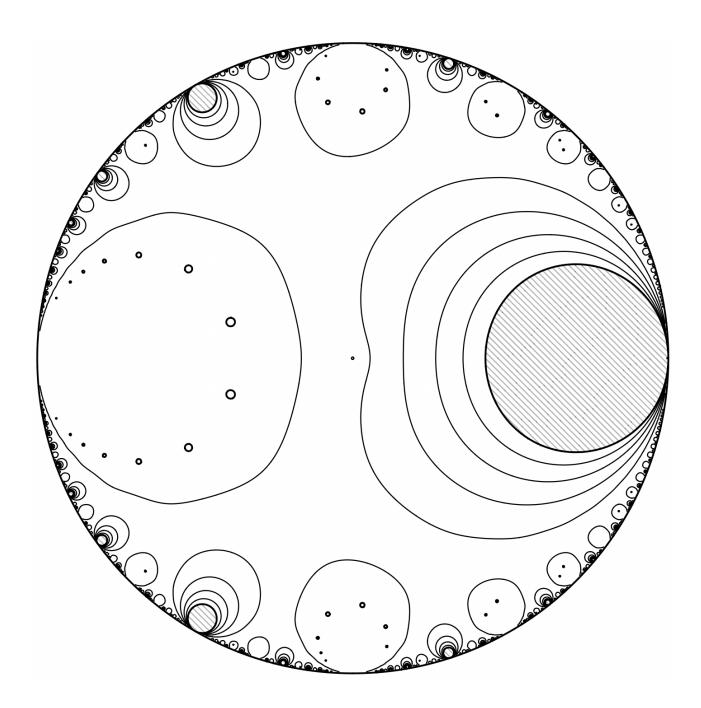
\includegraphics[width=0.55\textwidth]{assets/fig/_page_200_Picture_2.jpeg}
  \caption{阴影区域包含满足 \(|h(z)| \geq e^{20}\) 且靠近 cusp \(z = e^{2\pi i p/q}\) （其中 q 是奇数）的部分. 其他等高线为在 \(|h(z)| \in \{1, e^4, e^8, e^{12}, e^{16}\}\) 上的等高线，以及绕 -1/72 在 \(|h(z) + 1/72| = 1/200\) 的原像等高线.}\label{fig:A.0.3}
\end{figure}

构造 \(\Omega\) 的基本想法是选择一个以原点为中心、半径排除了在 \(z = \pm i\) 附近的 -1/72 
原像的圆周, 
并且然后（近似地）从 \(\Omega\) 中移除以下内容:
\begin{itemize}
  \item[(1)] 该圆周与靠近 z = 1 的 horoball 的交集.
  \item[(2)] 在靠近 z = -1 的 horoball 附近, 从该圆周到剩下的 -1/72 原像的狭缝（slits）.
\end{itemize}

Riemann 映射定理保证了对于任何此类区域 \(\Omega\) 均存在一个 \(\psi(x)\). 
然而, 我们还希望选择一个具有如下显式形式的 \(\psi(x)\), 
以便能够对 \eqref{eq:A.0.2} 进行严格的估计. 
因此在实际中, 我们选择近似该区域的简单显式函数. 
\(\Omega\) 的构造是非常定制化的, 
并且（对我们而言）完全不清楚如何在所有的 \(\Omega\) 
上最小化 \eqref{eq:A.0.2}, 
除了从我们的经验中可以说, 我们相信我们的构造与最优选择相差不远. 
我们最终选择的 \(\Omega\) 展示在图 A.4.5 中（该图还具有 \(\log |h(z)|\) 的更详细地形图）.

\subsection{关于圆弧二角形（Lunes）的准备知识}\label{sec:A.1}

设 D(c, R) 表示以 c 为中心、半径为 R 的圆盘. 
固定 c > 1, 并考虑映射:
\[ f(z,c) = z \cdot \frac{(c^2+1) + (c^2-1)z}{(c^2-1) + (c^2+1)z}. \]
该映射具有如下性质：它是一个从圆弧二角形 L(c) 
到单位圆盘的、将 z = 0 映射为 0 的共形同构, 
其中该二角形组成如下:
\[ L(c) := \mathbf{D} \setminus \mathbf{D} \cap D\left(-\frac{c^2+1}{c^2-1}, \frac{2c}{c^2-1}\right). \]
也就是单位圆盘减去两个在 \(|z| = 1\) 处以直角相交的圆盘的交集. 
（这保证了存在一个显式且初等的共形映射）. 
右侧圆周的“最内侧”点是点:
\[ -\frac{c^2+1}{c^2-1} + \frac{2c}{c^2-1} = -\frac{c-1}{c+1}. \]
在极限 \(c \to \infty\) 下, 该点趋近于 -1, 
并且区域 L(c) 趋近于整个圆盘, \(f(z)\) 趋近于 z. 
函数 f(z) 具有由下式给出的显式逆映射:
\begin{equation}\label{eq:A.1.1}
h(z,c) = \frac{z(1+c^2) - 1 - c^2 + \sqrt{(1+c^2)^2(1+z)^2 - 16c^2z}}{2(c^2 - 1)},
\end{equation}
并因此 L(c) 的共形半径为:
\begin{equation}\label{eq:A.1.2}
\frac{c^2 - 1}{c^2 + 1}.
\end{equation}

\subsection{吞噬区域（Gobbles）}\label{sec:A.2}

我们在定理 A 或 C 的证明中并未使用本节的围道, 
而是用我们在下文第 A.3 节中考虑的狭缝与圆弧二角形的组合代替了它们. 
然而, 它们在第 6.8 节定理 2.8.4 的证明中被使用了. 
此外, 我们的初版论证确实采用了它们, 
并且它们为提供在其他例子上的基准测试提供了便利的围道, 
而且也比我们稍微有些定制化的狭缝使用更灵活.

假设我们希望移除两个对称相反的圆盘, 它们并不一定具有相同的大小. 
在这种情况下没有容易表述的简单共形映射. 
然而, 作为第一步近似, 我们可能先移除一个圆盘, 
然后移除另一个. 我们定义:
\[ \operatorname{Gob}(z, e, f) := h(-h(z, f), e). \]
使用公式 \eqref{eq:A.1.1}, 这具有一个稍微有些杂乱、但完全显式的形式.

\begin{definition}\label{def:A.2.1}
在 \(\mathbf{D}\) 内部、伴随参数 \(r \in (0, 1]\), \(e \in (1, \infty]\), 以及 \(f \in (1, \infty]\) 
的吞噬区域是 \(\mathbf{D} = D(0, 1)\) 在映射:
\[ \operatorname{Gob}(r, e, f) : \mathbf{D} \to \mathbf{C}, z \mapsto r \cdot \operatorname{Gob}(z, e, f) \]
下的像. \(\triangle\)
\end{definition}

一个核心性质是, 对于极宽范围的参数, 
该吞噬区域在视觉上与 \(D(0,1)\) 中两个圆盘的补集是无法区分的, 
而在同一时间其又明显更显式、从而更容易计算. 
由显式公式, 我们很容易获得:

\begin{lemma}\label{lem:A.2.2}
以 z = 0 为中心的 \(\operatorname{Gob}(r, e, f)(\mathbf{D})\) 的共形半径等于:
\[ r \cdot \frac{(e^2-1)(f^2-1)}{(e^2+1)(f^2+1)}. \]
\end{lemma}

\subsection{狭缝（Slits）}\label{sec:A.3}

对于实数 r \(\in (0, 1)\), 从
\[ (\mathbf{D},0) \xrightarrow{\simeq} (\mathbf{D} \setminus (-1,-r],0) \]
的一个共形同构由下式定义的函数 \(\operatorname{Slit}(z, r)\) 给出:
\begin{equation}\label{eq:A.3.1}
\frac{(r+1)^2 - 2(r-1)^2 z + (r+1)^2 z^2 + (1+r)(-1+z)\sqrt{(1+r)^2 - 2(1-6r+r^2)z + (1+r)^2 z^2}}{8rz}
\end{equation}
\[ = \frac{4r}{(1+r)^2} z + \frac{8r(1-r)^2}{(1+r)^4} z^2 + \frac{4(1-r)^2 r(3-14r+3r^2)}{(1+r)^6} z^3 + \dots \]
特别地, \(\mathbf{D} \setminus (-1, -r]\) 在原点处的共形半径等于:
\begin{equation}\label{eq:A.3.2}
|\operatorname{Slit}'(0,r)| = \frac{4r}{(1+r)^2}.
\end{equation}

我们包含了对映射 \eqref{eq:A.3.1} 导出过程的一个概述. 
起步点是评述：有理变换 \(z \mapsto z/(1+z)^2\) 将我们的狭缝圆盘 \(\mathbf{D} \setminus (-1, -r]\) 
共形同构地映射为 \(\mathbf{P}^1 \setminus [-(1-r)^2/r, 1/4]\) 的倒数像. 
现在, 实轴上的线段 \([A, B] \subset \mathbf{R}\) 具有等于其长度四分之一的超限直径（外半径）. 
这已经证明了关于共形大小的公式 \eqref{eq:A.3.2}, 
因为 Riemann 映射球 \(\mathbf{P}^1 = \mathbf{C} \cup \{\infty\}\) 
中一个紧子集 K 补集在原点处的共形半径等于 K 超限直径的倒数. 
对于实际的 Riemann 映射 \eqref{eq:A.3.1}, 
我们通过观察到线段补集 \(\mathbf{P}^1 \setminus [A, B]\) 的、从 \(\infty\) 的逆 Riemann 映射由一个平方根函数给出而继续进行:
\[ \mathbf{P}^1 \setminus [A, B] \xrightarrow{\simeq} \mathbf{H}, \quad z \mapsto i\sqrt{(z-A)/(z-B)}, \quad \infty \mapsto i, \]
其逆映射为 \(z \mapsto \frac{A+Bz^2}{1+z^2}\). 
在应用 Cayley 变换 \(\mathbf{H} \xrightarrow{\simeq} \mathbf{D}\), \(z \mapsto (z-i)/(z+i)\) （其逆映射为 \(z \mapsto i(1+z)/(1-z)\)）的前提下, 
我们到达了合成的 Riemann 映射 \eqref{eq:A.3.1}.

\subsection{组合多重狭缝以及圆弧二角形}\label{sec:A.4}

假设我们希望移除四个狭缝以及一个二角形. 
在这种情况下没有容易表述的简单共形映射. 
然而, \eqref{eq:A.1.1} 以及 \eqref{eq:A.3.1} 中的两个共形映射都具有如下性质： 
它们在圆周的“大多数”点上（也就是在偏离二角形以及狭缝的点处） 
都可以被恒等映射 \(z \mapsto z\) 很好地近似. 
因此, 构造此类映射的一种非常原始的方式仅仅是依次复合这些映射. 
为此, 我们考虑以下函数:
\[ G(z) := -R \cdot h\left(-e^{2\pi i\theta_1} \cdot \operatorname{Slit}\left(e^{2\pi i\theta_2} \cdot \operatorname{Slit}\left(e^{2\pi i\theta_3} \operatorname{Slit}\left(e^{2\pi i\theta_4} \cdot \operatorname{Slit}\left(z, r_1\right), r_2\right), r_3\right), r_4\right), c\right). \]

我们固定第一个参数 R=77/100 以确保初始圆周仅包含 -1/72 在 -1 附近 horoball 中的原像, 
以及我们只需要排除 4 个此类原像. 
我们还固定了二角形参数 c=75/10, 该参数测量了我们在 z=1 附近移除的（近似）horoball. 
角度参数 \(\theta_i\) 允许我们“对齐”狭缝, 
使得它们包含了这些原像, 
并且长度参数 \(r_i\) 允许我们最小化这些狭缝的长度, 
使得它们不会越过我们希望排除的原像. 
最终的参数选择如下:
\[ R = \frac{77}{100}, \qquad c = \frac{75}{10}, \]
\[ r_1 = \frac{91}{100}, \qquad r_2 = \frac{6188}{10000}, \qquad r_3 = \frac{55515}{100000}, \qquad r_4 = \frac{772}{1000}, \]
\begin{equation}\label{eq:A.4.1}
\begin{aligned}
\theta_1 &= \frac{7977}{100000}, \qquad \theta_2 = \frac{11543}{100000}, \\
\theta_3 &= \frac{3525}{100000}, \qquad \theta_4 = -\frac{783}{10000}.
\end{aligned}
\end{equation}

这些参数选自一个临时的计算, 该计算使狭缝的端点尽可能地靠近四个参数. 
由于在数值上无法选择这些参数使得坏原像精确地位于这些狭缝上, 
我们最终定义:
\begin{equation}\label{eq:A.4.2}
\psi(z) = G\left(\frac{995}{1000} \cdot z\right).
\end{equation}

通过限制到这个开圆盘上, 我们不仅仅移除了（弯曲的）狭缝, 
还移除了开区域, 这使得证明坏原像已被排除变得非常容易. 
计算 \(\psi(z)\) 的共形半径（使用 \eqref{eq:A.1.2} 以及 \eqref{eq:A.3.2}）是非常简单的, 
它等于:
\[ |\psi'(0)| = \frac{995}{1000} \cdot R \cdot \frac{c^2 - 1}{c^2 + 1} \cdot \prod_{i=1}^{4} \frac{4r_i}{(1 + r_i)^2} \]
\begin{equation}\label{eq:A.4.3} 
= \frac{5448339453535586608000000000}{8658833407565631122430056127} = 0.6292232680... 
\end{equation}


召回 \(h: \mathbf{D} \to \mathbf{C}\) 在 \(q \in \mathbf{D}\) 下由 \(-256q \prod_{n=1}^{\infty} (1+q^n)^{24}\) 给出. 
上面选择的参数 \(r_i\) 以及 \(\theta_i\) 保证了以下结论成立:

\begin{lemma}\label{lem:A.4.4}
映射 \(\varphi := h \circ \psi : \mathbf{D} \to \mathbf{C}\) 具有唯一的 -1/72 原像.
\end{lemma}

\begin{proof}
存在一个原像满足 \(x = 0.0000541829...\). 
但人们可以通过回到 \(\mathbf{H}\) 来（以任意精度）确定其他原像, 
并且然后由 \(\Gamma_0(2)\) 的作用获得了其他的原像. 
在 \(z = \pm i\) 附近的区域（近似一 horoball）中的原像的绝对值至少为:
\[ 0.782767... > R = \frac{77}{100}. \]
最接近的其他原像位于 z = -1 附近的 horoball 附近； 
但对参数 \(r_i\) 以及 \(\theta_i\) 的精确选择确保了它们位于 \(\psi\) 像的外部, 
这可以通过简单的数值计算来予以证实.
\end{proof}

围道 \(\psi(\mathbf{T})\) 画在图~\ref{fig:A.4.5} 中. 
不对称性是由于我们使用了四个单狭缝映射的连续复合, 
而不是一次性移除所有四个狭缝.

\begin{figure}[htbp]
  \centering
  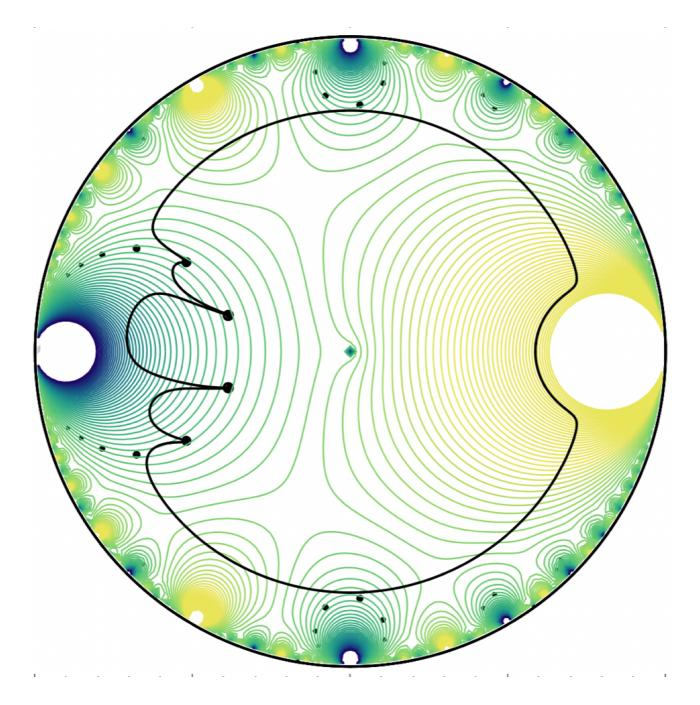
\includegraphics[width=0.45\textwidth]{assets/fig/_page_203_Figure_7.jpeg}
  \caption{\(\psi(z)\) 在 \(|z| = 1\) 处的像，以及 \(-1/72\) 在 h 下的原像，以及 \(\log |h|\) 在等差数列上的等高线. 颜色方案在黄色（正大值）与蓝色（负小值）之间转换.}\label{fig:A.4.5}
\end{figure}

\begin{remark}\label{rem:A.4.6}
我们对常数的选择仅反映了寻找一个“可行”而非最美观的例子的原理. 
这无疑存在一些改进的空间, 
但由于这不是必需的, 我们并未尝试优化这些选择——无论如何, 我们预计这两个方面的改进都将是非常温和的. \end{remark}

\subsection{针对 \texorpdfstring{$L(2, \chi_{-3})$}{L(2, \textbackslash{}chi\_\{-3\})} 问题的围道}\label{sec:A.5}

伴随我们对 \(\psi(z)\) 在等式 \eqref{eq:A.4.2} 中的特定选择, 我们现在定义:
\[ \varphi(z) = h(\psi(z)), \]
该映射在 \(\mathbf{D}\) 上是一致连续的, 
以及足够显式以至于可以进行严格的数值估计. 
我们随后最终获得了估计:
\[ \iint_{\mathbf{T}^2} \log |\varphi(z) - \varphi(w)| \, \mu_{\text{Haar}}(z) \mu_{\text{Haar}}(w) = 11.844\dots \]
以及因此, \eqref{eq:A.0.2} 被上估计为:
\begin{equation}\label{eq:A.5.1}
\frac{11.845}{\log\left(256 \cdot \frac{5448339453535586608000000000}{8658833407565631122430056127}\right) - \left(\frac{27}{80} + \frac{191}{49}\right)} = 13.9938 \dots < 14.
\end{equation}

\begin{remark}[Basic Remark A.5.2]\label{rem:A.5.2}
即使做出了我们所有的改进, 在增加积分之前, 
对于定理 A 或 C, 我们所能达到的最佳边界也都在 9 以上； 
我们现在给出其中一些数值. 
考虑定理 2.5.1 在下述情况下的基本应用. 
我们考虑在 \(\mathbf{P}^1 \setminus \{0, 1, \infty\}\) 域中的函数 \(A_i(x)\) 对于 i = 1, ..., 9. 
（在此, 前五个函数在第 10 节中显式给出, 
以及四个函数 \(A_6(x), ..., A_9(x)\) 通过那一节的变换对应于 \(B_6(z), ..., B_9(z)\). 
注意, 这些最后的四个函数只有在我们的三个周期之间存在 \(\mathbf{Q}\)-线性关系时才存在.） 
对于下式考虑定理 2.5.1:
\[ \mathbf{b} := \begin{pmatrix} 0 & 1 & 1 & 1 & 1 & 1 & 1 & 1 & 1 \\ 0 & 0 & 1 & 1 & 1 & 1 & 1 & 1 & 1 \end{pmatrix}^{\mathrm{t}} \]
并因此有 \(\sigma_1 = 0, \sigma_2 = 1\); \(\sigma_3 = \dots = \sigma_9 = 2\), 
以及:
\[ \tau(\mathbf{b}) = \frac{1 \cdot 0 + 3 \cdot 1 + (5 + 7 + 9 + 11 + 13 + 15 + 17) \cdot 2}{81} = \frac{157}{81}. \]
正如在注记 9.0.20 中解释的那样, 
如果我们使用与等式 \eqref{eq:A.4.2} 中相同的、但被拉回到 \(X(2)\) 域中的围道, 
积分项以及共形半径项都加倍了. 
等价地, 它们保持相同而 \(\tau\) 项减半了. 
因此我们在该情况下获得的对应边界为:
\begin{equation}\label{eq:A.5.3}
\frac{11.844...}{5.081...-2\cdot 157/81} = 9.833... < 10,
\end{equation}
这已经很接近但并没有形成矛盾, 因为该项并不小于 9. 
虽然这可以被稍微精细化（使用 Bost--Charles 积分以及修改围道）, 
但在不引入增加积分的前提下, 通过我们的方法似乎不太可能达到直接的矛盾； 
参见示例 7.4.9 以及 7.5.9. \end{remark}

\subsection{针对对数问题的围道}\label{sec:A.6}

我们完全可以使用与上文相同的围道来完成定理 C 的证明, 
除了伴随着一个稍微更差的常数之外. 
遵循第 14.4 节的论证, 
只要寻找满足 \(\psi\) 像排除了 z 不是太小且 h(z) 位于 \(D(0, \varepsilon^2/16)\) 内以及 h(z) 位于 \(D(0, \varepsilon^{-1})\) 
之外的区域的 \(\varepsilon\) 就已足够. 
这导致了在 \(10^7\) 以及 \(10^8\) 之间对 \(\varepsilon\) 的选择. 
然而, 在对各种不同共形映射进行优化以及使用与上文相同的映射之间的一个妥协是：直接写下简单的二角形: 
如果我们取具有共形半径为 1287/2516 以及形式为
\[ \psi(z) = -\frac{3}{4}h\left(z, \frac{23}{10}\right) \]
的二角形, 那么 \(\psi(z)\) 的像排除了所有需要的圆盘以及满足 \(|h(z)| \ge 10^6\) 以及 \(|h(z)| \le 10^{-12}2^{-4}\) 
的区域（除了在 z=0 附近的原像之外）. 
在此情况下, 我们获得了估计边界:
\begin{equation}\label{eq:A.6.1}
\iint_{\mathbf{T}^2} \log |\varphi(z) - \varphi(w)| \, \mu_{\text{Haar}}(z) \mu_{\text{Haar}}(w) \sim 9.963\dots < 10,
\end{equation}
并且我们拥有非常容易的边界:
\begin{equation}\label{eq:A.6.2}
\frac{10}{\log\left(256 \cdot \frac{1287}{2516}\right) - \frac{1032659}{242760}} = 16.103... < 17,
\end{equation}
该边界被我们在第 14.5 节中用于定理 C 的证明. 
作为比较, 我们也可以估计重排积分:
\begin{equation}\label{eq:A.6.3}
\int_0^1 2t \cdot (\log |\varphi(e^{2\pi it})|)^* dt \sim 9.972...
\end{equation}
该边界也足以证明定理 C, 此时是通过仅具有对 [0, m] 平凡划分的定理 6.0.2 获得的.

关于 \(\psi(z)\) 的像以及满足 \(|h| \ge 10^6\) 以及 \(|h| \le 10^{-12}2^{-4}\) 的区域的图像画在图~\ref{fig:A.6.4} 中.

\begin{figure}[htbp]
  \centering
  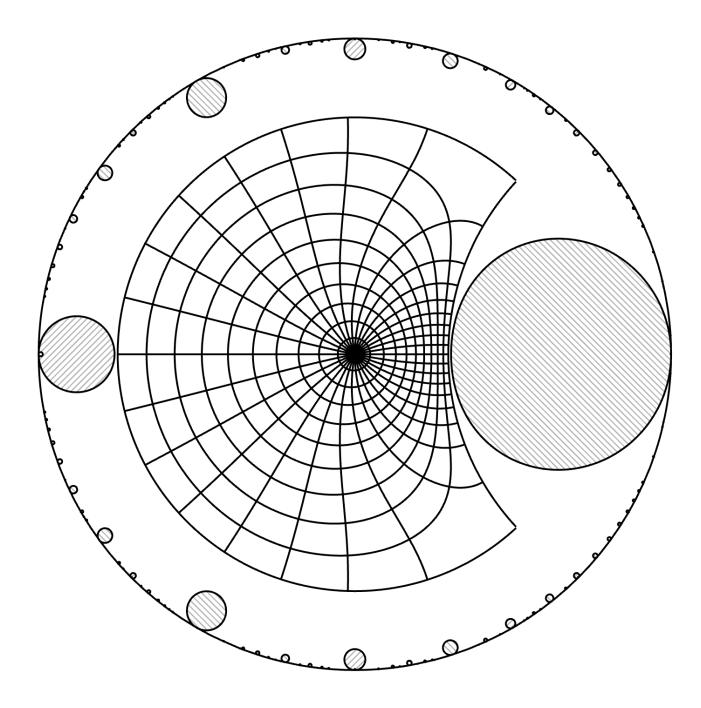
\includegraphics[width=0.45\textwidth]{assets/fig/_page_206_Figure_2.jpeg}
  \caption{\(|z| = 1\) 以及等高线在 \(\psi(z)\) 下的像，以及满足 \(|h| \geq 10^6\) 和 \(|h| < 10^{-12}2^{-4}\) 的区域（通过阴影的角度进行区分）.}\label{fig:A.6.4}
\end{figure}

% 引入附录 B 内容
\section{动态抽屉原理}\label{sec:B}

在本附录中, 我们在分母为正的条件下, 
为在 \(\mathbf{Q}(x)\) 上线性无关的形式函数集合 \(f_1, \ldots, f_m \in \mathbf{Q}[\![x]\!]\) 
（具有形式 \eqref{eq:2.2.1} 并且满足 \(\varphi, \varphi^* f_1, \ldots, \varphi^* f_m \in \mathcal{M}(\overline{\mathbf{D}})\) 
在闭单位圆盘 \(\overline{\mathbf{D}}\) 的一个邻域内是联立亚纯的） 
给出了基本 holonomy 边界的简短新证明:
\begin{equation}\label{eq:B.0.1}
m \le \frac{2T(\varphi)}{\log|\varphi'(0)| - b_1 - \dots - b_r}.
\end{equation}
在此处,
\begin{equation}\label{eq:B.0.2}
T(\varphi) := \int_{\mathbf{T}} \log^{+} |\varphi| \, \mu_{\text{Haar}} + \sum_{\substack{\rho \in \mathbf{D} \\ \text{poles of } \varphi}} \log \frac{1}{\rho}
\end{equation}
是亚纯映射 \(\varphi\) 的 Nevanlinna 特征函数（亚纯极点按其重度计算）.

这基于 Perelli 以及 Zannier \cite{PZ84} 的一个动态抽屉原理想法, 
正如他们在该文献的引理 1 中所陈述的那样. 
它可以被视为第 7 节中 Bost 技术的更初等形式, 
它既是后者的引入也是一种替代方案, 
并且也指向我们的伴随论文 \cite{CDT24}, 
在其中这些想法得到了进一步的研究. 
我们根据第 2.12 节中的解剖将证明分为三个步骤.

\subsection{评估模}\label{sec:B.1}

假设我们拥有一组在 \(\mathbf{Q}(x)\) 上线性无关的、具有 \eqref{eq:2.2.1} 形式的函数 \(f_1(x), \dots, f_m(x) \in \mathbf{Q}[\![x]\!]\), 
使得 \(\varphi(z) \in \mathbf{C}[\![z]\!]\) 以及每个形式幂级数 \(f_i(\varphi(z)) \in \mathbf{C}[\![z]\!]\) 
都是闭复单位圆盘 \(|z| \le 1\) 邻域内的亚纯函数芽. 
（在用 \(\varphi(\rho z)\) 对于某些仍然满足 \(\rho|\varphi'(0)| > e^{b_1 + \dots + b_r}\) 的 \(\rho < 1\) 
代替 \(\varphi(z)\) 的前提下, 
拥有这个稍微大一些的圆盘并不损失一般性.） 
我们引入两个正整数参数 D 以及 T, 
并考虑集合:
\begin{equation}\label{eq:B.1.1}
\mathcal{I}_D(T) := \left\{ (Q_1, \dots, Q_m) \in \mathbf{Z}[x] : Q_i(x) = \sum_{j=0}^{D-1} c_{i,j} x^j, c_{i,j} \in [0, T) \cap \mathbf{Z} \right\},
\end{equation}
其基数为:
\begin{equation}\label{eq:B.1.2}
\#\mathcal{I}_D = T^{mD}.
\end{equation}

根据对 m 个形式幂级数 \(f_i(x) \in \mathbf{Q}[\![x]\!]\) 
所假设的 \(\mathbf{Q}(x)\)-线性无关性, 
\(\mathbf{Z}\)-模评估映射
\begin{equation}\label{eq:B.1.3}
\psi_D: \mathbf{Z}[x]_{\deg < D}^{\oplus m} \hookrightarrow \mathbf{Q}[\![x]\!], \qquad (Q_1, \dots, Q_m) \mapsto \sum_{i=1}^m Q_i(x) f_i(x) \in \mathbf{Q}[\![x]\!]
\end{equation}
是单射. 
因此, 该映射下的像
\[ \mathcal{O}_D := \psi_D(\mathcal{I}_D) \subset \mathbf{Q}[\![x]\!] \]
也具有基数:
\begin{equation}\label{eq:B.1.4}
\#\mathcal{O}_D = \#\mathcal{I}_D = T^{mD}.
\end{equation}

在秩为 mD 的自由 \(\mathbf{Z}\)-模 \eqref{eq:B.1.3} 中, 我们定义消逝过滤跳跃:
\begin{equation}\label{eq:B.1.5}
r_D^{(n)} := \dim_{\mathbf{Q}} \left\{ \left( \psi_D^{-1} \left( x^n \mathbf{Q} [\![x]\!] \right) \otimes \mathbf{Q} \right) / \left( \psi_D^{-1} \left( x^{n+1} \mathbf{Q} [\![x]\!] \right) \otimes \mathbf{Q} \right) \right\}.
\end{equation}
它们位于 \(\{0,1\}\) 中, 因为单射线性映射 \(\psi_D\) 诱导了一个线性单射:
\[ \left(\psi_D^{-1}\left(x^n\mathbf{Q}[\![x]\!]\right)\otimes\mathbf{Q}\right)/\left(\psi_D^{-1}\left(x^{n+1}\mathbf{Q}[\![x]\!]\right)\otimes\mathbf{Q}\right)\hookrightarrow x^n\mathbf{Q}[\![x]\!]/x^{n+1}\mathbf{Q}[\![x]\!]\cong\mathbf{Q}\cdot x^n \]
到一维 \(\mathbf{Q}\)-向量空间中. 
在另一方面, 我们有:
\begin{equation}\label{eq:B.1.6}
\sum_{n=0}^{\infty} r_D^{(n)} = \dim_{\mathbf{Q}} \psi_D^{-1} \mathbf{Q} [\![x]\!] = mD.
\end{equation}
因此, 存在一个大小为 mD 的、我们的辅助函数在 \(x = 0\) 处的可能消逝阶数集合:
\begin{equation}\label{eq:B.1.7}
\left\{ n \in \mathbf{N} : \exists (Q_1, \dots, Q_m) \in \mathbf{Z}[x]_{\deg < D}^{\oplus m}, \operatorname{ord}_{x=0} \left( \sum_{i=1}^m Q_i(x) f_i(x) \right) = n \right\}
\end{equation}
\[ = \left\{ 0 \le u(1) < u(2) < \dots < u(mD) \right\}. \]
它们的设定仅依赖于模 \eqref{eq:B.1.3} 
——换句话说, 仅依赖于 \(f_1, \ldots, f_m\) 以及参数 D, 
——而不依赖于参数 T, 该参数在后文中仍保持自由选择. 
（参数 T 将被选为依赖于过滤跳跃 \eqref{eq:B.1.7} 的任意足够大的整数.）

这完成了第 2.12 节的步骤 (i).

\subsection{抽屉原理}\label{sec:B.2}

对于步骤 (ii)，在临界条件 \(|\varphi'(0)| > e^{b_1 + \dots + b_r}\) 下，我们来测量辅助函数 \(F(x)\) 的 Taylor 级数递归地依赖于其初始系数串的趋势。

我们可以通过乘积 \(\prod_{p=1}^{mD} \gamma_p\) 来上估计输出基数 \(\#\mathcal{O}_D\)，其中 \(\gamma_p\) 是在共享一个公共先前系数串 \((\beta_0, \beta_1, \ldots, \beta_{u(p)-1})\) 的任意输出函数 \(F(x) = \sum_{k=0}^{\infty} \beta_k x^k\) 集合中、不同 \(x^{u(p)}\) 系数 \(\beta_{u(p)} \in \mathbf{Q}\) 的最大可能数量的上估计：
\[ \forall (\beta_0, \dots, \beta_{u(p)-1}) \in \mathbf{Q}^{u(p)}, \]
\[ \# \left\{ \beta \in \mathbf{Q} : \exists (Q_1, \dots, Q_m) \in \mathcal{I}_D, \sum_{i=1}^m Q_i(x) f_i(x) - \sum_{k=0}^{u(p)-1} \beta_k x^k = \beta x^{u(p)} + O(x^{u(p)+1}) \right\} \leq \gamma_p. \]

此时，利用整性条件 \eqref{eq:2.6.2} 可知，所有这些有理数 \(\beta \in \mathbf{Q}\) 实际上都属于由所需分母类型所给出的 \(\mathbf{Z}\)-模中：
\[ \beta \in \frac{1}{[1,\ldots,b_1 \cdot u(p)]\cdots[1,\ldots,b_r \cdot u(p)]}\mathbf{Z}. \]
因此，如果 \(A_p \in \mathbf{R}^{>0}\) 使得任意两个此类系数 \(\beta\) 的差的绝对值都在区间 \([-A_p, A_p]\) 内，那么我们可以取：
\begin{equation}\label{eq:B.2.1}
\gamma_p := 1 + 2A_p \cdot [1, \dots, b_1 u(p)] \cdots [1, \dots, b_r u(p)] = 1 + A_p \cdot e^{(b_1 + \dots + b_r)u(p) + o(u(p)) + O(1)}
\end{equation}
作为在给定 \((\beta_0, \dots, \beta_{u(p)-1})\) 的情况下 \(\beta_{u(p)}\) 所有可能输出值的总边界。这一步模仿了 Perelli 和 Zannier 的动态抽屉原理 \cite[第 2 节引理 1]{PZ84}（或译为动态盒原理）。

\subsection{对最低阶系数的丢番图分析}\label{sec:B.3}

对于 \(A_p\) 的边界，在解析上来自于使用多变量亚纯一致化映射 \(\varphi\)。考虑将 \(\varphi\) 表示为两个在闭单位圆盘 \(\overline{\mathbf{D}}\) 上收敛且满足 \(u(0) = 1\) 的幂级数 \(u\) 与 \(v\) 的商的任意表示：\(\varphi = v/u\)。令 \(h\) 为 \(\overline{\mathbf{D}}\) 上的一个满足 \(h(0) = 1\) 且使得对每个 \(i = 1, \ldots, m\)，\(hf_i\) 在 \(\overline{\mathbf{D}}\) 上全纯的收敛幂级数。为了书写简单，我们在下文中设 \(n := u(p)\)。任意两个上述输出函数 \(F_1(x)\) 和 \(F_2(x)\)，若其在 \(x = 0\) 处的 Taylor 级数一致直到 \(O(x^n)\)，且其相应的 \(x^n\) 系数分别为 \(\beta^{(1)}\) 和 \(\beta^{(2)}\)，那么它们将使得函数
\[ V(z) := h(z)u(z)^D \cdot (F_1(\varphi(z)) - F_2(\varphi(z))) \]
在闭单位圆盘 \(\overline{\mathbf{D}}\) 的一个邻域上是全纯的（收敛的），并且其领先阶项 \(\varphi'(0)^n(\beta^{(1)}-\beta^{(2)})z^n+O(z^{n+1})\) 可以根据 Cauchy 公式表示为在 \(|z|=1\) 上的围道积分：
\begin{equation}\label{eq:B.3.1}
\varphi'(0)^n(\beta^{(1)} - \beta^{(2)}) = \int_{\mathbf{T}} \frac{V(z)}{z^{n+1}} \,\mu_{\text{Haar}}.
\end{equation}

通过对被积函数的上确界进行估计，我们可以将 \(A_p\) 取为下式底部的上界：
\begin{equation}\label{eq:B.3.2}
\begin{aligned}
\left| \beta^{(1)} - \beta^{(2)} \right| &\le |\varphi'(0)|^{-n} \cdot \sup_{\mathbf{T}} |V| \\
&\le |\varphi'(0)|^{-u(p)} \cdot T \left( \sup_{\mathbf{T}} \max(|u|, |v|) \right)^{D} \cdot mD \cdot \sup_{\mathbf{T}} |h \cdot \varphi^* f_i| =: A_p,
\end{aligned}
\end{equation}
其中采用了 \(n := u(p)\)。

对于 \(\prod_{p=1}^{mD} \gamma_p\) 种可能输出，我们获得了总输出基数 \(T^{mD} = \#\mathcal{O}_D\) 的如下上估计：
\[
\begin{aligned}
\le \prod_{p=1}^{mD} \Big\{ &1 + T \exp\left(-\left(\log|\varphi'(0)| - b_1 - \dots - b_r + o(1)\right) u(p)\right) \\
&+ D \sup_{\mathbf{T}} \log \max(|u|, |v|) + \log D + O_{m,h}(1)\Big\}.
\end{aligned}
\]

此时，我们考虑上述不等式在 \(T \to \infty\) 下的渐近行为。更具体地，我们选择一个足够大的 \(T\)，使得该乘积的所有 \(mD\) 个因子都 \(\ge 2\)。利用当 \(x \ge 1\) 时的平凡不等式 \(1 + x \le 2x\)，并在等式两边消去共同出现的 \(T^{mD}\)，在取对数后，我们得到：
\[
\begin{aligned}
&-(\log |\varphi'(0)| - b_1 - \dots - b_r)(1 - o(1)) \sum_{p=1}^{mD} u(p) \\
&+ mD^2 \sup_{\mathbf{T}} \log \max(|u|, |v|) + O(D \log D) \ge -mD \log 2 - O_{m,h}(D).
\end{aligned}
\]

由于 \(0 \le u(1) < u(2) < \cdots < u(mD)\) 是非负整数的严格单增序列，我们有：
\begin{equation}\label{eq:B.3.3}
\sum_{p=1}^{mD} u(p) \ge \sum_{n=0}^{mD-1} n = \binom{mD}{2}.
\end{equation}

由此，我们导出：
\begin{equation}\label{eq:B.3.4}
(1-o(1))\binom{mD}{2}\left(\log|\varphi'(0)|-b_1-\dots-b_r\right) \le mD^2 \sup_{\mathbf{T}}\log\max(|u|,|v|)+O_{m,h}(D),
\end{equation}
在 \(D \to \infty\) 的渐近下，这最终过滤为如下算术 holonomy 边界：
\begin{equation}\label{eq:B.3.5}
m \le \frac{2\sup_{\mathbf{T}}\log\max(|u|,|v|)}{\log|\varphi'(0)| - b_1 - \dots - b_r}.
\end{equation}

该结论对于满足 \(u(0) = 1\) 的任何亚纯商表示 \(\varphi = v/u\) 均成立。Nevanlinna 的一个著名引理（参见 \cite[第 VII.1.4 节]{Nev70}），基于 Poisson--Jensen 公式中 canonical Blaschke 乘积以及对数分解 \(\log = \log^+ - \log^-\)，在开圆盘 \(\mathbf{D}\) 上构造了一个满足 \(u(0) = 1\)且满足 \(\sup_{\mathbf{D}} |u|\) 和 \(\sup_{\mathbf{D}} |v|\) 均由 \(\exp(T(\varphi))\) 所控制的商表示 \(\varphi = v/u\)。稍微放大（扩张）半径，对于任何 \(\varepsilon > 0\)，我们都可以获得一个商表示 \(\varphi = v/u\)，其定义在上述分析所需的闭圆盘 \(\mathbf{D}\) 的某个开邻域上，且满足 \(\sup_{\mathbf{T}} |u|\) and \(\sup_{\mathbf{T}} |v|\) 均由 \(\exp(T(\varphi) + \varepsilon)\) 所控制。这便完成了边界 \eqref{eq:B.0.1} 的证明。\(\square\)

\bibliographystyle{alpha}
\bibliography{bib/references}

\end{document}
